% The packages used here are just a sample. You may need others, and may not need some of these. It doesn't hurt to leave them in, unless they start to conflict with other packages you've added. Chapter 2 has example code for equations, figures, tables, citations, abbreviations, etc. If there are sections labeled 'optional' that you don't want, just comment them out. -jg

\documentclass[reqno,12pt,oneside]{report} % right-side equation numbering, 12 point font, print one-sided 
%\documentclass[reqno,12pt,twoside,openright]{report} % right-side equation numbering, 12 point font, print two-sided, Chapters start on odd pages. Rackham only accepts one-sided, so this is for personal printings.

\usepackage{rac}         % Use Rackham thesis style file
\usepackage{setspace}    % Allows you to specify the line spacing
\onehalfspacing %or \doublespaceing
\usepackage{tikz}
\usetikzlibrary{arrows}

\usepackage[font=small,labelfont=bf]{caption}

\usepackage{amstext,amsmath,amssymb,amsthm}
\usepackage{graphicx}
%\usepackage{algorithm,algorithmic}
\usepackage[figure,linesnumbered,ruled,vlined]{algorithm2e}
%\usepackage{algpseudocode}
\usepackage{booktabs}
\usepackage[tight]{subfigure}
\usepackage{comment, color, xcolor}
\usepackage{bbm}

%Colors
\definecolor{boxgrey}{HTML}{F1F1F1}
\definecolor{boxdarkgrey}{HTML}{919191}
\definecolor{boxblue}{RGB}{149,181,206}

%TOC
\newcommand{\hiddensubsection}[1]{
    \stepcounter{subsection}
    \subsection*{\Alph{chapter}.\arabic{section}.\arabic{subsection}\hspace{1em}{#1}}
}
\newcommand{\hiddensection}[1]{
    \stepcounter{section}
    \subsection*{\Alph{chapter}.\arabic{section}\hspace{1em}{#1}}
}

%Boxes
\newlength\mytemplen
\newsavebox\mytempbox

\makeatletter
\newcommand{\mybluebox}{%
    \@ifnextchar[%]
       {\@mybluebox}%
       {\@mybluebox[0pt]}}

\def\@mybluebox[#1]{%
    \@ifnextchar[%]
       {\@@mybluebox[#1]}%
       {\@@mybluebox[#1][0pt]}}

\def\@@mybluebox[#1][#2][#3]#4{
    \sbox\mytempbox{#4}%
    \mytemplen\ht\mytempbox
    \advance\mytemplen #1\relax
    \ht\mytempbox\mytemplen
    \mytemplen\dp\mytempbox
    \advance\mytemplen #2\relax
    \dp\mytempbox\mytemplen
    \fcolorbox{black}{#3}{\hspace{1em}\usebox{\mytempbox}\hspace{1em}}}

\makeatother

%Equations, aligned, and itemize
\newcommand{\beq}{\begin{equation}}
\newcommand{\eeq}{\end{equation}}
\newcommand{\be}{\begin{equation*}}
\newcommand{\ee}{\end{equation*}}
\newcommand{\ba}{\begin{aligned}}
\newcommand{\ea}{\end{aligned}}
\newcommand{\bea}{\begin{equation}\begin{aligned}}
\newcommand{\eea}{\end{aligned}\end{equation}}
\newcommand{\bit}{\begin{itemize}}
\newcommand{\eit}{\end{itemize}}

% Detection stuff
\newcommand{\detgtrless}{\overset{H_1}{\underset{H_0}{\gtrless}}}
\newcommand{\siggtrless}{\overset{\text{sig}}{\underset{\text{not sig}}{\gtrless}}}
\newcommand{\convas}{\overset{\textrm{a.s.}}{\longrightarrow}}
\newcommand{\indicator}{\mathbbm{1}}

%Algorithm Stuff
%\renewcommand{\algorithmicrequire}{\textbf{Input:}}
%\renewcommand{\algorithmicensure}{\textbf{Output:}}

%Statements
\newtheorem{prop}{Proposition}[section]
\newtheorem{conj}{Conjecture}[section]
\newtheorem{Th}{Theorem}[section]
\newtheorem{Corr}{Corollary}[section]
\newtheorem{Assum}{Assumption}[section]
\newtheorem{Def}{Definition}[section]
\newtheorem{Conj}{Conjecture}[section]
\newtheorem{Remark}{Remark}[section]
\newtheorem{Lem}{Lemma}[section]

% text abbrevs
\newcommand{\eg}{{\it e.g.}}
\newcommand{\ie}{{\it i.e.}}
\newcommand{\naive}{na\"{\i}ve }
\newcommand{\Naive}{Na\"{\i}ve }
\newcommand{\naively}{na\"{\i}vely }

%Random Matrix
\newcommand{\keff}{k_\text{eff}}
\newcommand{\keffhat}{\widehat{k}_\text{eff}}
\newcommand{\kuse}{k_{\text{useful}}}

% std math stuff
\newcommand{\ones}{\mathbf 1}
\newcommand\reals{\ensuremath{\mathbb{R}}}
\newcommand{\integers}{{\mbox{\bf Z}}}
\newcommand\complex{\ensuremath{\mathbb{C}}}
\newcommand{\symm}{{\mbox{\bf S}}}  % symmetric matrices
\newcommand{\Prob}[1]{\mathbb{P}\left({#1}\right)}
\newcommand{\E}[1]{\mathbb{E}\left[{#1}\right]}

% lin alg stuff
\newcommand{\Span}{\mathop{\bf span}}
\newcommand{\range}{{\mathcal R}}
\newcommand{\nullspace}{{\mathcal N}}
\newcommand{\Rank}{\mathop{\bf rank}}
\newcommand{\Tr}{\mathop{\bf tr}}
\newcommand{\cond}{\mathop{\bf cond}}
\newcommand{\diag}{\mathop{\bf diag}}
\newcommand{\blkdiag}{\mathop{\bf blkdiag}}
\newcommand{\lambdamax}{\lambda_{\rm max}}
\newcommand{\lambdamin}{\lambda_{\rm min}}

% probability stuff

\newcommand{\var}{\mathop{\bf var}} % variance
% not sure why we have \Expect and \Prob but \var ???

% convexity & optimization stuff
\newcommand{\Co}{\mathop {\bf conv}} % convex hull
\newcommand{\argmin}{\mathop{\rm argmin}}
\newcommand{\argmax}{\mathop{\rm argmax}}
\newcommand{\epi}{\mathop{\bf epi}}
%\newcommand{\hypo}{\mathop{\bf hypo}}

% sup and inf that look OK in saddle-point form!
%\newcommand{\ourinf}{\mathop{\raisebox{0ex}[0ex][.4ex]{\,inf\,}}}
%\newcommand{\oursup}{\mathop{\raisebox{0ex}[0ex][.4ex]{\,sup\,}}}
\newcommand{\ourinf}{\mathop{\,\mathrm{inf}\, {\rule[-.5ex]{0ex}{0ex}}}}
\newcommand{\oursup}{\mathop{\,\mathrm{sup}\, {\rule[-.5ex]{0ex}{0ex}}}}
%makes latex believe that inf and sup both extend .4ex below
%the baseline

\newcommand{\dist}{\mathop{\bf dist}}
\newcommand{\vol}{\mathop{\bf vol}} % volume
\newcommand{\Card}{\mathop{\bf card}} % cardinality
\newcommand{\sign}{\mathop{\bf sign}}

\newcommand{\dom}{\mathop{\bf dom}} % domain
\newcommand{\aff}{\mathop{\bf aff}} % affine hull
\newcommand{\cl}{\mathop{\bf cl}} % closure
\newcommand{\intr}{\mathop{\bf int}} % interior
\newcommand{\relint}{\mathop{\bf rel int}} % relative interior
\newcommand{\bd}{\mathop{\bf bd}} % boundary

%why do we have the following but not \nust?
\newcommand{\xst}{x^\star}
\newcommand{\lambdast}{\lambda^\star}

% defs for cones & generalized inequalities
% these seem kind of awkward; should fix some day
% rewrite them to use args?
\newcommand{\geqK}{\mathrel{\succeq_K}}
\newcommand{\gK}{\mathrel{\succ_K}}
\newcommand{\leqK}{\mathrel{\preceq_K}}
\newcommand{\lK}{\mathrel{\prec_K}}
\newcommand{\geqKst}{\mathrel{\succeq_{K^*}}}
\newcommand{\gKst}{\mathrel{\succ_{K^*}}}
\newcommand{\leqKst}{\mathrel{\preceq_{K^*}}}
\newcommand{\lKst}{\mathrel{\prec_{K^*}}}
\newcommand{\geqL}{\mathrel{\succeq_L}}
\newcommand{\gL}{\mathrel{\succ_L}}
\newcommand{\leqL}{\mathrel{\preceq_L}}
\newcommand{\lL}{\mathrel{\prec_L}}
\newcommand{\geqLst}{\mathrel{\succeq_{L^*}}}
\newcommand{\gLst}{\mathrel{\succ_{L^*}}}
\newcommand{\leqLst}{\mathrel{\preceq_{L^*}}}
\newcommand{\lLst}{\mathrel{\prec_{L^*}}}


\newenvironment{algdesc}%
   {\begin{list}{}{%
    \setlength{\rightmargin}{0\linewidth}%
    \setlength{\leftmargin}{.05\linewidth}}%
    \sffamily\small
    \item[]{\setlength{\parskip}{0ex}\hrulefill\par%
    \nopagebreak{}}}%
   {{\setlength{\parskip}{-1ex}\nopagebreak\par\hrulefill} \end{list}}

\newenvironment{colm}{\left[\begin{array}{c}}{\end{array}\right]}
\newenvironment{colv}{\left(\begin{array}{c}}{\end{array}\right)}


\usepackage{accents,array}

% CCA things
\newcommand{\xI}{x_1}
\newcommand{\xII}{x_2}
\newcommand{\xIhat}{\widehat{x}_1}
\newcommand{\xIIhat}{\widehat{x}_2}
\newcommand{\yI}{y_1}
\newcommand{\yII}{y_2}
\newcommand{\RI}{R_{11}}
\newcommand{\RII}{R_{22}}
\newcommand{\RIII}{R_{12}}
\newcommand{\RIhat}{\widehat{R}_{11}}
\newcommand{\RIIhat}{\widehat{R}_{22}}
\newcommand{\RIIIhat}{\widehat{R}_{12}}
\newcommand{\wI}{w_1}
\newcommand{\wII}{w_2}
\newcommand{\Creg}{C_{\text{reg}}}
\newcommand{\Creghat}{\widehat{C}_{\text{reg}}}
\newcommand{\Cregtil}{\widetilde{C}_{\text{reg}}}
\newcommand{\Ckcca}{C_{\text{kcca}}}
\newcommand{\Ckccatil}{\widetilde{C}_{\text{kcca}}}

\newcommand{\twr}{{\sf TW}_\reals}
\newcommand{\twc}{{\sf TW}_\complex}
\newcommand{\sx}{s_{x,i}}
\newcommand{\sy}{s_{y,i}}
\newcommand{\zx}{z_{x,i}}
\newcommand{\zy}{z_{y,i}}
\newcommand{\Zx}{Z_x}
\newcommand{\Zy}{Z_y}
\newcommand{\Ux}{U_x}
\newcommand{\Uy}{U_y}
\newcommand{\Vx}{V_x}
\newcommand{\Vy}{V_y}
\newcommand{\Pxy}{P_{xy}}
\newcommand{\kx}{k_x}
\newcommand{\ky}{k_y}
\newcommand{\kxhat}{\widehat{k}_x}
\newcommand{\kyhat}{\widehat{k}_y}
\newcommand{\khatcca}{\widehat{k}_{\text{cca}}}
\newcommand{\khaticca}{\widehat{k}_{\text{icca}}}
\newcommand{\Uxhat}{\widehat{U}_x}
\newcommand{\Uyhat}{\widehat{U}_y}
\newcommand{\Sigxhat}{\widehat{\Sigma}_x}
\newcommand{\Sigyhat}{\widehat{\Sigma}_y}
\newcommand{\Sigxtil}{\widetilde{\Sigma}_x}
\newcommand{\Sigytil}{\widetilde{\Sigma}_y}
\newcommand{\Vxhat}{\widehat{V}_x}
\newcommand{\Vyhat}{\widehat{V}_y}
\newcommand{\Uxtil}{\widetilde{U}_x}
\newcommand{\Uytil}{\widetilde{U}_y}
\newcommand{\Vxtil}{\widetilde{V}_x}
\newcommand{\Vytil}{\widetilde{V}_y}
\newcommand{\Uxcir}{\accentset{\circ}{U}_x}
\newcommand{\Uycir}{\accentset{\circ}{U}_y}
\newcommand{\Vxcir}{\accentset{\circ}{V}_x}
\newcommand{\Vycir}{\accentset{\circ}{V}_y}
\newcommand{\Sigxcir}{\accentset{\circ}{\Sigma}_x}
\newcommand{\Sigycir}{\accentset{\circ}{\Sigma}_y}
\newcommand{\kapcir}{\accentset{\circ}{\kappa}}
\newcommand{\xii}{x_i}
\newcommand{\yii}{y_i}
\newcommand{\Tx}{\Theta_x}
\newcommand{\Ty}{\Theta_y}
\newcommand{\Txhat}{\widehat{\Theta}_x}
\newcommand{\Tyhat}{\widehat{\Theta}_y}
\newcommand{\tx}{\theta^{(x)}}
\newcommand{\ty}{\theta^{(y)}}
\newcommand{\Kxy}{K_{xy}}
\newcommand{\Kxytil}{\widetilde{K}_{xy}}
\newcommand{\Uktil}{U_{\widetilde{K}}}
\newcommand{\Vktil}{V_{\widetilde{K}}}
\newcommand{\Uktilhat}{\widehat{U}_{\widetilde{K}}}
\newcommand{\Vktilhat}{\widehat{V}_{\widetilde{K}}}
\newcommand{\kxy}{k^{xy}}
\newcommand{\defeq}{=:}
\newcommand{\Rxx}{R_{xx}}
\newcommand{\Ryy}{R_{yy}}
\newcommand{\Rxy}{R_{xy}}
\newcommand{\Rxxhat}{\widehat{R}_{xx}}
\newcommand{\Ryyhat}{\widehat{R}_{yy}}
\newcommand{\Rxyhat}{\widehat{R}_{xy}}
\newcommand{\wx}{w_x}
\newcommand{\wy}{w_y}
\newcommand{\wxt}{\widetilde{w}_x}
\newcommand{\wyt}{\widetilde{w}_y}
\newcommand{\wxicca}{\widehat{w}_x^{\text{icca}}}
\newcommand{\wyicca}{\widehat{w}_y^{\text{icca}}}
\newcommand{\wxticca}{\widetilde{w}_x^{\text{icca}}}
\newcommand{\wyticca}{\widetilde{w}_y^{\text{icca}}}
\newcommand{\wxhaticca}{\widehat{w}_x}
\newcommand{\wyhaticca}{\widehat{w}_y}
\newcommand{\Ccca}{C_{\text{cca}}}
\newcommand{\Cccahat}{\widehat{C}_{\text{cca}}}
\newcommand{\Ciccahat}{\widehat{C}_{\text{icca}}}
\newcommand{\rank}{\text{rank}}
\newcommand{\taucca}{\tau_{\text{cca}}^\alpha}
\newcommand{\tauicca}{\tau_{\text{icca}}^\alpha}
\newcommand{\simiid}{\overset{\text{i.i.d.}}{\sim}}
\newcommand{\rhocca}{\rho_\text{cca}}
\newcommand{\rhohatcca}{\widehat{\rho}_\text{cca}}
\newcommand{\rhohaticca}{\widehat{\rho}_\text{icca}}
\newcommand{\rhoeff}{k_{\text{eff}}^{xy}}

\newcommand{\Clrcca}{C_{\text{lrcca}}}

\newcommand{\Rmcca}{C_{\text{mcca}}}
\newcommand{\Rmccahat}{\widehat{R}_{\text{mcca}}}
\newcommand{\Rmccatil}{\widehat{R}_{\text{imcca}}}
\newcommand{\Ucir}{\accentset{\circ}{U}}
\newcommand{\Vcir}{\accentset{\circ}{V}}

\newcommand{\Sww}{S_{ww}}
\newcommand{\Swy}{S_{wy}}
\newcommand{\Syw}{S_{yw}}
\newcommand{\Sxx}{S_{xx}}
\newcommand{\Syy}{S_{yy}}
\newcommand{\Sxy}{S_{xy}}
\newcommand{\Syx}{S_{yx}}
\newcommand{\wxhat}{\widehat{w}_x}
\newcommand{\wyhat}{\widehat{w}_y}
\newcommand{\ttu}{\widetilde{\widetilde{u}}}

\newcommand{\iccap}{ICCA\texttt{+} }
\newcommand{\iccaps}{ICCA\texttt{+}}


\newcolumntype{C}{ >{\centering\arraybackslash} m{0.7in} }
\newcolumntype{D}{ >{\centering\arraybackslash} m{1in} }
\newcolumntype{E}{>{\centering\arraybackslash} m{2in}}
\newcolumntype{F}{>{\centering\arraybackslash} m{3in}}


\newcommand{\figwidth}{2.9in}

%%%%%%%%%%%%%%%%%%%%%%%%%%%%%%%%%%%%%%%%%%%%%%%%%%%%%%%%%%%%%%%%%%%%%%%%%%%%%%%

% If printing two-sided, this makes sure that any blank page at the 
% end of a chapter will not have a page number. 
\makeatletter
\def\cleardoublepage{\clearpage\if@twoside \ifodd\c@page\else
\hbox{}
\thispagestyle{empty}
\newpage
\if@twocolumn\hbox{}\newpage\fi\fi\fi}
\makeatother 

\begin{document}

% Title page as required by Rackham dissertation guidelines
\titlepage{Informative Data Fusion:\\ Beyond Canonical Correlation Analysis}{Nicholas A. Asendorf}{Doctor of Philosophy}
{Electrical Engineering: Systems}{2015}
{Assistant Professor Raj Rao Nadakuditi, Chair\\
 Assistant Professor Laura Balzano\\
 Professor Alfred O. Hero III\\
 Associate Professor Rada Mihalcea}


% Begin the front matter as required by Rackham dissertation guidelines
\initializefrontsections

% Optional Frontispiece % TODO
\frontispiece{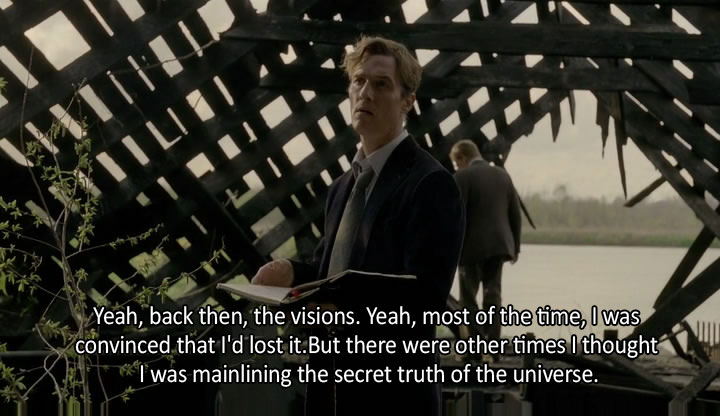
\includegraphics[width=5in]{figures/secret_truth.jpg}}

% Optional, but recommended, Copyright page
\copyrightpage{Nicholas A. Asendorf}

% Page numbering. If you don't include a frontispiece or copyright page, you'll need to change this for two-sided printing.
\makeatletter
\if@twoside \setcounter{page}{4} \else \setcounter{page}{1} \fi
\makeatother
 
% Optional Dedication page
\dedicationpage{For my grandmothers Josephine Asendorf and Doris Evashko, in memoriam.}

% Optional Acknowledgements page
\startacknowledgementspage
I would first like to thank my adviser Prof. Raj Nadakuditi. Thank you for allowing me to
be one of your very first students. Your ideas and passion for research truly do
inspire. Thank you for teaching me how to pick the low hanging fruit, how to see the
strucutre in complicated problems, and how to always ``push it through''.

I would specifically like to thank my committee members for their inspiring conversations
and courses over the past 5 years. Prof. Rada Mihalcea, thank you for your information
retrieval course. I enjoyed chatting with you about the possible applications of
correlation analysis to such problems. Prof. Laura Balzano, thank you for coming to the
University of Michigan; I consider myself lucky that your arrival was timed so perfectly
with my dissertation. You have been a wonderful addition to EE:S and I am excited to learn
from your work in the years to come. Prof. Alfred Hero, thank you for our numerous
conversations over the years at conferences and MURI funding meetings. Your insights
always helped to deepen my understanding of the problems that we solve. I would also like
to thank my undergraduate research advisers at the University of Maryland, Prof. Jonathan
Simon and Prof. Adam Hsieh, for first introducing me to the research process.

Thank you to all the members of the Nadakuditi group - Curtis Jin, Raj Tejas Suryaprakash,
Himanshu Nayar, Brian Moore, Arvind Prasadan, and David Hiskens. Specifically, I would
like to thank Raj Tejas for his help with the analysis of missing data and Brian Moore for
his wonderfully elegant hacks of \textsc{MATLAB}.

Thank you to all the members of the Graduate Student Council and SPeecs organizing
committee. Specifically I would like to thank Kevin Xu, Michael Allison, and Mads
Almassalkhi for their leadership and passing down the needed graduate student lore. Thank
you also to the advanced technology group at 3M. I thoroughly enjoyed my internship last
summer and am looking forward to working with you all over the next years. I would also
like to thank the National Basketball Association for providing an escape from research. 

To my high school friends Alex McArthur, John Vaccacio, Allison Seyler, Andy Mellon, Matt
Keel, Alec Brown, Chris Rowe, Mike Hyle, and Jason Pribble: thank you for always being
there to remind me of my roots. While I have only sporadically been able to spend time
with you in person over the last five years, I valued every minute of it. Alex - thank you
for teaching me to always trust your decisions. Allison, Alec, Andy, Chris and Jason -
thank you for humoring me by listening to my academic ramblings. Matt, Mike, and John
- thank you for always keeping me guessing. 

To my friends from the University of Maryland, Jaime Gomez, Austin Myers, Sarah Saslow,
Kyle Smith, Andy Peters, and Nick Gagliolo: thank you for always being there and for
appreciating the alma mater as much as I do - ``steadfast in loyalty''. Jaime - I will
never forget all of the memories at Courtyards. Thank you for teaching me how to play
tennis, bridge, and spades. Thank you for teaching me about nuclear physics and for
always providing logical advice when I needed it.  Sarah - thank you for always providing
a listening ear when I needed it. Thank you for all of the football weekends as we watched
Michigan and Northwestern in graduate school. Kyle - thank you for all of the late night
card games and video games, for teaching me about fire protection engineering, and all of
the weekends that we were able to see each other since graduation. Austin - thank you for
being an awesome roomate and colleague, for your goofy sense of humor,
and all of the conversations that we had. Nick - thank you for keeping me sane through all
of the courses, group projects, exams, and gemstone activities. Andy - thank you for all
of the sports conversations and going to all of the Maryland games with me over the years.

To my friends and colleagues at the University of Michigan, Rob Vandermeulen, Madison
McGaffin, Mitchell Thomas Hellman Young, Matthew Prelee, Steve Schmitt, Paul Ozog, Eric
Uthoff, Pat O'Keefe, and Mike Henry: thank you for making graduate school fun. Paul, Eric,
and Pat - thank you for all the first and second year hang outs that got us through our
coursework. Steve - thank you for all the walk-and-talks, letting me borrow your sitting
ball, and teaching me about the midwest. Rob - thank you for introducing me to your many
hobbies; you have really broadened my world view. Matt - thank you for all of the
walk-and-talks, football trips, sports arguments, board game nights, and long runs. Mike -
thank you for being really good at trivia and the many fun nights at your place. Mitch -
thank you for teaching me how to brew, being a Linux whisperer, teaching me about flux,
and for the HoM. Madison - thank you for all of the walk-and-talks, entertaining my OCD
Pathfinder ideas, teaching me how to make bread, being a word-o-mancer, and all of the
memories contained at HoM.

To my girlfriend Christie VanTongeren - thank you for all of your support over the past
three years. Thank you for your understanding for all of the late nights over the past
months and always listening. Thank you teaching me all of your expert cooking
techniques and for all of the movie, bowling, game, and trivia nights. Thank you
for sharing my values but always challenging me to be better. I am so excited for
Minneapolis.

I would like to thank all of the EECS support staff who made my job easier over the years
at the University of Michigan. Special thanks go to our graduate coordinators Becky
Turanski, Beth Stalnaker, and Rachel Young Antoun. Thank you for always being there to
answer questions, keeping me on track, and brightening up my day. Thank you also to our wonderful
4th floor staff Beth Lawson, Anne Pace, and Shelly Feldkamp. You make our jobs so
easy by hiding the many  complicated intricacies of the funding process. I also
greatly appreciated your kindness and support over the last four years. It was always a
pleasure to catch up with you.

I would like to thank my piano teacher of eight years, Shirley Elsroad, and organ teacher Lee
Pogue. Thank you for teaching the joy of the piano and organ and teaching me to express
myself though them in my own voice. I will always fondly remember my lessons with the both
of you. I would also like to thank Prof. Steven Ball for teaching me how to play the
carillons at the University of Michigan. Thank you for teaching me how to perfume the Ann
Arbor air with music.

Finally, I would like to thank my mother Nancy, father David, and sister Amy. I
would not be where I am today without your support, encouragement, and amazing
parenting. I know that not everyone is as lucky as I was to be born into such a supportive
enviornment and for that, words cannot describe my gratitude. This thesis is a testament
to your parenting skills. 

\label{Acknowledgements}

% Table of contents, list of figures, etc.
\tableofcontents     % Required
\listoffigures       % Required if there is more than one figure
\listoftables        % Required if there is more than one table
%\listofmaps          % Required if there is more than one map
\listofappendices    % Required if there is more than one appendix
%\listofabbreviations % Optional. Abbreviations should be stored in a file named abbr.tex

% Optional in-dissertation Abstract Page
\startabstractpage
{Informative Data Fusion:\\ Beyond Canonical Correlation Analysis}{Nicholas
  A. Asendorf}{Chair: Raj Rao Nadakuditi}
%\abstract{We analyze the performance of a matched subspace detector (MSD) where the test signal vector is assumed to reside in an unknown, low-rank $k$ subspace that must be estimated from finite, noisy, signal-bearing training data. Under both a stochastic and deterministic model for the test vector, subspace estimation errors due to limited training data degrade the performance of the standard plug-in detector, relative to that of an oracle detector. To avoid some of this performance loss, we utilize and extend recent results from random matrix theory (RMT) that precisely quantify the quality of the subspace estimate as a function of the eigen-SNR, dimensionality of the system, and the number of training samples. We exploit this knowledge of the subspace estimation accuracy to derive from first-principles a new RMT detector and to characterize the associated ROC performance curves of the RMT and plug-in detectors. Using more than the a critical number of \textit{informative} components, which depends on the training sample size and eigen-SNR parameters of training data, will result in a performance loss that our analysis quantifies in the large system limit.  We validate our asymptotic predictions with simulations on moderately sized systems.
}
We analyze the performance of a matched subspace detector (MSD) where the test signal vector is assumed to reside in an unknown, low-rank $k$ subspace that must be estimated from finite, noisy, signal-bearing training data. Under both a stochastic and deterministic model for the test vector, subspace estimation errors due to limited training data degrade the performance of the standard plug-in detector, relative to that of an oracle detector. To avoid some of this performance loss, we utilize and extend recent results from random matrix theory (RMT) that precisely quantify the quality of the subspace estimate as a function of the eigen-SNR, dimensionality of the system, and the number of training samples. We exploit this knowledge of the subspace estimation accuracy to derive from first-principles a new RMT detector and to characterize the associated ROC performance curves of the RMT and plug-in detectors. Using more than the a critical number of \textit{informative} components, which depends on the training sample size and eigen-SNR parameters of training data, will result in a performance loss that our analysis quantifies in the large system limit.  We validate our asymptotic predictions with simulations on moderately sized systems.

\label{Abstract}

\startthechapters 
% The individual files for each of the chapters are put here.
% Save each chapter of your thesis to a seperate tex file
% and then use the \input command to include this file in your
% thesis.  For instance you can save a file to "intro.tex" and 
% then type Multi-modal data fusion is a ubiquitous problem in signal processing and machine
learning. In many applications, we have access to multiple datasets, possibly of different
modalities, each of which describe some feature of the system. This setup is becoming
increasingly common today as data collection becomes cheaper and easier. We are no longer
limited by the amount or variety of data that we can collect, but instead by how quickly
and accurately we can process such a wide variety of data.

The underlying assumption in such settings is that each dataset contains signals that are
correlated with signals of the other datasets. Correlation analysis algorithms hope to
leverage this fact to extrude these correlated signals \textit{jointly} from the datasets
more accurately than from the individual datasets alone. Of course, every application has
a different goal. Sometimes we want to detect the presence of the correlated
signals. Other times, we may wish to predict one modality from the other. In other
applications, we may desire to classify or cluster observations. Despite the differing
objectives, all of these applications rely on the ability to accurately detect and extract
the correlated signals between the datasets. This thesis focuses on developing
theoretically justified, robust correlations analysis algorithms to use as a
pre-processing step before learning algorithms that perform data fusion, as
motivated by Figure \ref{fig:data_fusion}.

\begin{figure}
\begin{center}  
    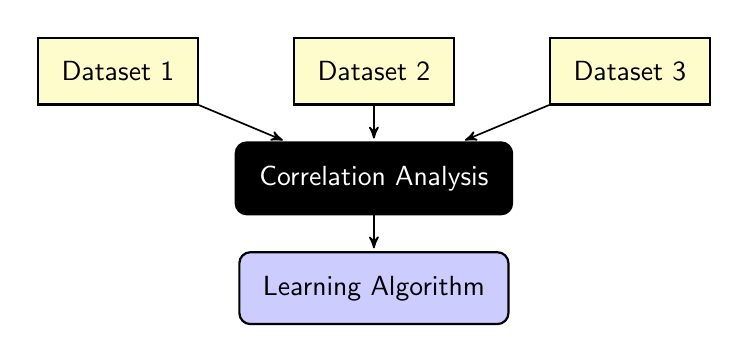
\begin{tikzpicture}[
      font=\sffamily, every matrix/.style={ampersand replacement=\&,column sep=3ex,row
      sep=3ex}, dataset/.style={draw,thick,fill=yellow!20,inner sep=.3cm},
      sink/.style={dataset,rounded corners,fill=black, text=white},
      app/.style={dataset,rounded corners,fill=blue!20}, dots/.style={gray,scale=2},
      to/.style={->,>=stealth',shorten >=1pt,semithick,font=\sffamily\footnotesize}, every
      node/.style={align=center}]

      \matrix{ \node[dataset] (dataset1) {Dataset 1}; \& \node[dataset] (dataset2)
        {Dataset 2}; \& \node[dataset] (dataset3) {Dataset 3}; \\

        \& \node[sink] (blackbox) {Correlation Analysis}; \& \\

        \& \node[app] (application) {Learning Algorithm}; \& \\ };

      \draw[to] (dataset1) -- (blackbox); \draw[to] (dataset2) -- (blackbox); \draw[to]
      (dataset3) -- (blackbox); \draw[to] (blackbox) -- (application);

    \end{tikzpicture}
    \caption{Illustration of multi-modal data fusion}
    \label{fig:data_fusion}
\end{center}
\end{figure}


\section{Canonical Correlation Analysis (CCA)}

\subsection{What is it? What is it not?}

Canonical correlation analysis (CCA) is a joint dimensionality reduction algorithm for
exactly two datasets that finds a linear transformation for each dataset such that the
correlation between the two transformed feature sets is maximized
\cite{hotelling1936relations}. CCA, however, \textit{is not} a data fusion algorithm. CCA
returns two linear transformations and a set of correlations. In this light, CCA is
extremely similar to principle component analysis (PCA), which returns a linear
transformation that accounts for the directions of largest possible variance in a
dataset. These principle components are typically used as features vectors in a variety of
machine learning algorithms. Just as PCA is a dimensionality reduction algorithm and not
the final machine learning algorithm that uses the principle components, CCA is a joint
dimensionality reduction algorithm whose dimensionality reduction ensures that datasets
are maximally correlated in their reduced spaces. These maximally correlated features may
then be used however a learning algorithm desires. 

The solution to CCA is easily found by solving a quadratic optimization problem. This
solution is a closed form expression relying on the singular value decomposition (SVD) of
a matrix product involving the covariance matrices of each dataset and the
cross-covariance between the two datasets. As these covariance matrices are rarely known
\textit{a priori}, practical uses of CCA rely on substituting sample covariance matrices
formed from training data, which we call empirical CCA.

The performance of empirical CCA has been studied previously, but insufficiently. When the
number of training samples is large compared to the dimensions of the datasets, the
performance is well understood \cite{gunderson1997estimating}. When the number of training
samples is less than the sum of the dimension of each dataset (sample deficient regime),
\cite{pezeshki2004empirical} proves that empirical CCA completely breaks down and always
reports a perfect correlation between the datasets. 

This extremely undesirable characteristic of empirical CCA has lead many to abandon CCA as
a reliable statistical analysis technique. Pezeshki, L.L. Scharf et al. argue that in this
sample deficient regime
\begin{quote}
  ... the \textcolor{red}{empirical canonical correlations are defective and
    may not be used} as     estimates of canonical correlations between random
  variables.\cite{pezeshki2004empirical}
\end{quote}
Similarly, Ge et al. conclude that
\begin{quote}
... CCA provide(s) \textcolor{red}{reliable information} about spatial
    correlations existing among pairs of data sets \textcolor{red}{only when SNRs ... are
    reasonably high, and the sample support is significantly larger than the data
    dimensions.}\cite{ge2009does}
\end{quote}



\subsection{Variations on CCA}

Due to this undesirable breakdown of CCA in the low-sample high-dimensionality regime,
many researchers proposed variations of CCA to avoid this performance loss. Most notably,
\cite{nadakuditi2011fundamental} used recent results from random matrix theory to
demonstrate that this performance breakdown may be avoided by trimming the sample
covariance matrix estimates to only include informative components. This algorithm is the
crux of this thesis. We will study its performance and develop theoretical tools in order
to use it for real-world applications. Throughout the thesis, we use the ubiquitous
low-rank signal-plus-noise model for datasets \be X = UV^H + Z, \ee where
$X=[x_1,\dots,x_n]$ is our observed data matrix whose columns are individual
multidimensional observations, $U$ is a low-rank signal subspace, $V$ is a low-rank signal
matrix, and $Z$ is a noise matrix. Surprisingly, correlation analysis for this classical
low-rank signal-plus-noise model is not completely studied. This thesis seeks to complete
the discussion. Here, we briefly touch on other variations based on CCA that do not assume
the above linear low-rank signal-plus-noise model. Many of these algorithms are tuned for
a specific application or seek to avoid the performance loss of CCA in a certain regime.

Regularized CCA (RCCA) \cite{vinod1976canonical} adds a penalty term to the magnitude of
the canonical vectors. This results in adding a scaled copy of the identity matrix to the
sample covariance matrix of each dataset, which allows each matrix to be
inverted. Therefore, RCCA returns non-trivial results in the sample-deficient
regime. However, this approach introduces a parameter to the algorithm; the effect of this
parameter is not well studied. Other variations of RCCA, such as supervised
RCCA \cite{thum2014supervised}, fast RCCA \cite{cruz2014fast}, and a multi-block RCCA
\cite{tenenhaus2014regularized}, have also been proposed.

Kernel CCA (KCCA) \cite{akaho2006kernel} was proposed to deal with non-linear correlations
existing between datasets. However, KCCA also introduces regularization parameters so as
to not return trivial solutions (see \cite{welling2005kcca} for an excellent
derivation). Besides the choice of regularization parameter, there is also ambiguity in
the choice of the kernel function, which is a common problem among kernel methods. Other
variations of KCCA have also been proposed, such as penalized KCCA
\cite{waaijenborg2009correlating}, alpha-beta divergence \cite{mandal2013non}, and CCA
based on kernel target alignment \cite{chang2013canonical}. 

Sparse CCA \cite{hardoon2011sparse} finds linear transformations such that the number of
features used is minimized. This problem is often motivated by the need for interpretable
canonical vectors that is often driven by the application, such as in brain imaging
\cite{yan2014accelerating}. There are many variations on sparse CCA, typically motivated
by application or mathematical intrigue. Sun and Keates \cite{sun2013canonical} explore
CCA in the context of censoring, Shin and Lee examine sparse functional data
\cite{shin2015canonical}, Tao et al. consider joint sparse data in
\cite{tao2014exploring}, Gao et al. explore efficient sparse CCA for high-dimensional
data \cite{gao2014efficient}, and Zhang et al. extend the analysis to multi-class group
sparse CCA \cite{zhang2013binary}. Other formulations include a penalized decomposition
\cite{witten2009penalized}, Bayesian CCA via group sparsity \cite{klami2013bayesian}, and
recursive sparse CCA \cite{chu2013sparse}.

\subsection{Applications}

CCA and its variants are widely used in a variety of fields where multiple datasets
naturally arise, the most common of which is machine learning and computer vision. In
\cite{hardoon2004canonical}, CCA is used to learn semantics of multimedia content by
fusing image and text data. Related, \cite{dhillon2011multi} uses CCA to learn word
embeddings for supervised natural language processing tasks. CCA has been widely applied
to pose estimation \cite{melzer2001nonlinear,zhai2015instance}, as this is a natural
examples where we have multiple views (image) of the same object. Other computer vision
related tasks where correlation methods are natural fits include matching people across
cameras \cite{lisanti2014matching}, clustering social event images
\cite{ahsan2014clustering}, automatic image annotation \cite{hardoon2006correlation}, and
audio-visual speaker clustering \cite{chaudhuri2009multi}.

Medical analysis is another field where there are ripe opportunities for correlation
analysis due to the vast number of modalities (EEG, MRI, CT, fMRI, MEG, etc.). CCA is
often used to determine interactions, or connectivities, between brain areas in fMRI data
\cite{deleus2011functional,arbabshirani2010comparison,khalid2013improving,guccione2013functional}
and used to fuse fMRI, sMRI, and EEG data \cite{correa2010canonical}. CCA based methods
have also been used to examine genetic connections
\cite{lin2013identifying,seoane2014canonical,lin2013group}, relying heavily on sparse
methods due to the high dimensionality of gene data and need to interpret which genes are
``on''. CCA is also a popular way to detect frequencies in steady-state visual evoked
potential (SSVEP) in brain-computer interfaces (BCIs)
\cite{zhang2013l1,nakanishi2014enhancing,zhang2014frequency}. Still further, CCA is used
in de-noising and analysis of EEG, MEG and ECG data
\cite{spuler2013spatial,campi2013non,chen2014removal,kuzilek2014comparison}.

CCA also has roots in classical signal processing applications. The authors of
\cite{via2005canonical} apply CCA to to the common communications problem of blind
equalization of single-input multiple-output (SIMO) channels. Pezeshki et al.
\cite{pezeshki2006canonical} showed that the CCA coordinates are the correct coordinates
for low-rank Gauss-Gauss detection and estimation. Scharf and Thomas
\cite{scharf1998wiener} provide a wonderful exposition on using the canonical coordinates
for Wiener filters, transform coding, filtering, and quantizing. CCA and multiset CCA have
been used to achieve joint blind source separation (BSS) in \cite{li2009joint}. CCA has
also been applied to hyperspectral imaging \cite{nielsen2002multiset}, array processing
\cite{ge2009does}, Gaussian channel capacity \cite{scharf2000canonical}, and cognitive
radio networks \cite{manco2014kernel}.

Other fun and interesting applications include climatology, finance, and music. Todros and
Hero define a new measure transformed based CCA and show its utility on financial data in
\cite{todros2012measure}. Torres et al. \cite{torres2007finding} use sparse CCA to label
portions of musical songs with meaningful words or phrases. In the field of climatology,
CCA has been used to study sea temperatures \cite{wilks2014probabilistic}, forest planning
\cite{prera2014using}, and tropical cyclones \cite{steward2014assimilating}. Finally, I
would be remiss if I didn't share my personal favorite application of CCA to date: using
CCA to analyze bovine growth \cite{li2010canonical}.

\section{Contributions of this thesis}

In many of the application presented above, researchers either have access to many
samples, or have designed an algorithm tuned specifically for a their particular
application. This thesis considers the performance of empirical correlation algorithms in
the low-sample, high dimensional setting. These algorithms are not geared toward a
particular application but are general and may be applied to any application. We will
demonstrate, both theoretically and empirically, that multi-modal correlation analysis in
this regime is a possibility. We remark that statements labeled as theorems represent, to
the best of our knowledge, new results while important results from literature are labeled
as propositions or lemmas. Chapters II-III are self contained and may be read
independently. Chapters IV-X consider the problem of correlation analysis.

Chapters \ref{sec:chpt_msd} and \ref{sec:chpt_msd_exten} consider the classical problem of
matched subspace detectors. We use insights from random matrix theory on the accuracy of
subspace estimates to derive new, optimal detectors that demonstrate the sub-optimality of
the classical plug-in detectors that simply substitute maximum likelihood estimates for
unknown parameters. Under both a stochastic and deterministic data model, we argue that
only the \textit{informative} subspace components should be used in a detector. We extend
this analysis to the case where our observations may contain missing data.

In Chapters \ref{sec:chpt_cca_det} and \ref{sec:chpt_cca_vects}, we explore the
performance of CCA and re-derive informative CCA (ICCA). We demonstrate the extreme
sub-optimality of CCA in the low-sample, high dimensionality regime. Specifically, we
provide a statistical test for both CCA and ICCA that determines whether the correlations
returned by the algorithms do indeed represent a true underlying correlation in the
datasets. We prove when each of these statistics are consistent to showcase the
superiority of ICCA. We also provide an analogous statistical test and consistency theorem
to use when the datasets have missing data entries. We create 3 new real-world,
multi-modal datasets involving video and audio to verify the performance of ICCA. We then
showcase that the canonical vectors returned by ICCA are more accurate than the CCA
vectors in the low-sample regime. Finally, we provide a new algorithm for estimating the
canonical vectors that asymptotically optimal.

Next, we explore the performance of regularized CCA (RCCA) in Chapter
\ref{sec:chpt_rcca}. When the number of training samples is limited but correlation
analysis is still desired, a common strategy is to regularize CCA by adding a penalty to
the magnitude of the linear transformation. However, we demonstrate that setting the
regularization parameter to infinity results in the best performance. In fact, in this
setting, the solution to RCCA may be found by taking the SVD of the sample
cross-covariance matrix between the two datasets. We then predict the behavior of the
largest singular values of this cross-covariance matrix assuming a low-rank
signal-plus-noise model on the individual datasets. We argue that using the top singular
values of this cross-covariance matrix to detect correlations is sub-optimal because the
correlation coefficients are coupled with the individual data signal strengths.

Using a similar proof technique, we predict the behavior of the largest singular values of
the projection of low-rank signal plus noise matrices to a smaller dimension in Chapter
\ref{sec:chpt_svd_proj}. Specifically, we consider two types of projection matrices: one
with standard complex Gaussian entries and one with orthonormal columns. We are able to
provide a closed form expression for the largest singular values in the case where the
projection matrix is unitary. Through numerical simulations, we demonstrate the
superiority of the unitary projection matrix over the Gaussian projection matrix. The
unitary projection matrix can reliably detect the signals at a lower signal-to-noise ratio
than the Gaussian projection matrix. 

In Chapter \ref{sec:chpt_det_reg} we apply CCA and ICCA to the classical problems of
detection and regression. First, we consider the low-rank signal-versus-noise subspace
detection problem given two datasets. We prove that the standard likelihood ratio test
(LRT) detector may be written using the canonical basis returned by CCA. We show that when
using empirical parameter estimates, the CCA detector is extremely suboptimal but that the
ICCA detector is equivalent to the plug-in LRT detector. We then show that the classical
Gaussian regression problem may be written in terms of the CCA basis. However, similar to
the detection problem, empirical CCA degrades the performance significantly while ICCA
matches the classical plug-in detector. We show this via mean squared error prediction
plots.

We then consider the joint problems of image retrieval and image annotation in Chapter
\ref{sec:chpt_ia}. Correlation based methods are typically overlooked as solutions to such
problems due to the problems with CCA outlined in this thesis. We show that using ICCA to
solve these problems results in non-trivial solutions. We compare the performance of CCA
and ICCA on four different image-text datasets and describe the capabilities and
limitations of ICCA in this application. When the datasets contain multiple images of the
same objects and meaningful captions, ICCA is able to capture correlations between images
and text. However, ICCA fails to capture semantic meanings between documents and
captions. We argue that with clever feature engineering and improved NLP techniques,
correlation based methods may be relevant for image retrieval and image annotation.

Lastly, we consider multi-set CCA (MCCA) in Chapter \ref{sec:chpt_mcca}. Unfortunately,
unlike CCA, there is no clear objective function to use in an optimization problem;
Kettenring \cite{kettenring1971canonical} proposes five such objective functions. Nielsen
also provides a nice formulation of MCCA in \cite{nielsen1994analysis} where he proposes
four constraint functions.  We provide derivations for these 20 formulations, in both a
theoretical and empirical setting. We then choose to consider the MAXVAR problem as we are
able to directly apply our insights from ICCA to create an informative version of it,
which we call informative MCCA (IMCCA). We demonstrate the superior performance of IMCCA
on a real-world video dataset that we created. 
. 


\chapter{Introduction}\label{sec:intro}
Multi-modal data fusion is a ubiquitous problem in signal processing and machine
learning. In many applications, we have access to multiple datasets, possibly of different
modalities, each of which describe some feature of the system. This setup is becoming
increasingly common today as data collection becomes cheaper and easier. We are no longer
limited by the amount or variety of data that we can collect, but instead by how quickly
and accurately we can process such a wide variety of data.

The underlying assumption in such settings is that each dataset contains signals that are
correlated with signals of the other datasets. Correlation analysis algorithms hope to
leverage this fact to extrude these correlated signals \textit{jointly} from the datasets
more accurately than from the individual datasets alone. Of course, every application has
a different goal. Sometimes we want to detect the presence of the correlated
signals. Other times, we may wish to predict one modality from the other. In other
applications, we may desire to classify or cluster observations. Despite the differing
objectives, all of these applications rely on the ability to accurately detect and extract
the correlated signals between the datasets. This thesis focuses on developing
theoretically justified, robust correlations analysis algorithms to use as a
pre-processing step before learning algorithms that perform data fusion, as
motivated by Figure \ref{fig:data_fusion}.

\begin{figure}
\begin{center}  
    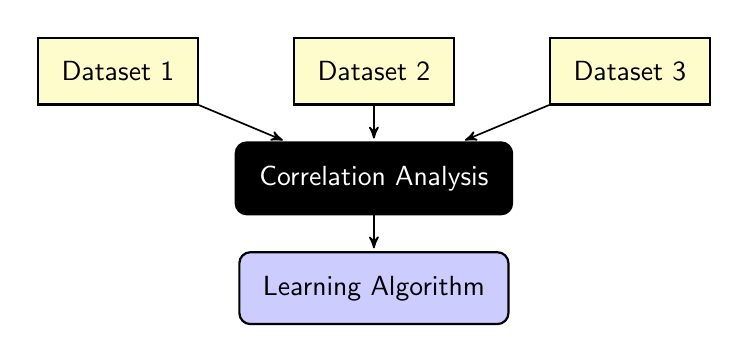
\begin{tikzpicture}[
      font=\sffamily, every matrix/.style={ampersand replacement=\&,column sep=3ex,row
      sep=3ex}, dataset/.style={draw,thick,fill=yellow!20,inner sep=.3cm},
      sink/.style={dataset,rounded corners,fill=black, text=white},
      app/.style={dataset,rounded corners,fill=blue!20}, dots/.style={gray,scale=2},
      to/.style={->,>=stealth',shorten >=1pt,semithick,font=\sffamily\footnotesize}, every
      node/.style={align=center}]

      \matrix{ \node[dataset] (dataset1) {Dataset 1}; \& \node[dataset] (dataset2)
        {Dataset 2}; \& \node[dataset] (dataset3) {Dataset 3}; \\

        \& \node[sink] (blackbox) {Correlation Analysis}; \& \\

        \& \node[app] (application) {Learning Algorithm}; \& \\ };

      \draw[to] (dataset1) -- (blackbox); \draw[to] (dataset2) -- (blackbox); \draw[to]
      (dataset3) -- (blackbox); \draw[to] (blackbox) -- (application);

    \end{tikzpicture}
    \caption{Illustration of multi-modal data fusion}
    \label{fig:data_fusion}
\end{center}
\end{figure}


\section{Canonical Correlation Analysis (CCA)}

\subsection{What is it? What is it not?}

Canonical correlation analysis (CCA) is a joint dimensionality reduction algorithm for
exactly two datasets that finds a linear transformation for each dataset such that the
correlation between the two transformed feature sets is maximized
\cite{hotelling1936relations}. CCA, however, \textit{is not} a data fusion algorithm. CCA
returns two linear transformations and a set of correlations. In this light, CCA is
extremely similar to principle component analysis (PCA), which returns a linear
transformation that accounts for the directions of largest possible variance in a
dataset. These principle components are typically used as features vectors in a variety of
machine learning algorithms. Just as PCA is a dimensionality reduction algorithm and not
the final machine learning algorithm that uses the principle components, CCA is a joint
dimensionality reduction algorithm whose dimensionality reduction ensures that datasets
are maximally correlated in their reduced spaces. These maximally correlated features may
then be used however a learning algorithm desires. 

The solution to CCA is easily found by solving a quadratic optimization problem. This
solution is a closed form expression relying on the singular value decomposition (SVD) of
a matrix product involving the covariance matrices of each dataset and the
cross-covariance between the two datasets. As these covariance matrices are rarely known
\textit{a priori}, practical uses of CCA rely on substituting sample covariance matrices
formed from training data, which we call empirical CCA.

The performance of empirical CCA has been studied previously, but insufficiently. When the
number of training samples is large compared to the dimensions of the datasets, the
performance is well understood \cite{gunderson1997estimating}. When the number of training
samples is less than the sum of the dimension of each dataset (sample deficient regime),
\cite{pezeshki2004empirical} proves that empirical CCA completely breaks down and always
reports a perfect correlation between the datasets. 

This extremely undesirable characteristic of empirical CCA has lead many to abandon CCA as
a reliable statistical analysis technique. Pezeshki, L.L. Scharf et al. argue that in this
sample deficient regime
\begin{quote}
  ... the \textcolor{red}{empirical canonical correlations are defective and
    may not be used} as     estimates of canonical correlations between random
  variables.\cite{pezeshki2004empirical}
\end{quote}
Similarly, Ge et al. conclude that
\begin{quote}
... CCA provide(s) \textcolor{red}{reliable information} about spatial
    correlations existing among pairs of data sets \textcolor{red}{only when SNRs ... are
    reasonably high, and the sample support is significantly larger than the data
    dimensions.}\cite{ge2009does}
\end{quote}



\subsection{Variations on CCA}

Due to this undesirable breakdown of CCA in the low-sample high-dimensionality regime,
many researchers proposed variations of CCA to avoid this performance loss. Most notably,
\cite{nadakuditi2011fundamental} used recent results from random matrix theory to
demonstrate that this performance breakdown may be avoided by trimming the sample
covariance matrix estimates to only include informative components. This algorithm is the
crux of this thesis. We will study its performance and develop theoretical tools in order
to use it for real-world applications. Throughout the thesis, we use the ubiquitous
low-rank signal-plus-noise model for datasets \be X = UV^H + Z, \ee where
$X=[x_1,\dots,x_n]$ is our observed data matrix whose columns are individual
multidimensional observations, $U$ is a low-rank signal subspace, $V$ is a low-rank signal
matrix, and $Z$ is a noise matrix. Surprisingly, correlation analysis for this classical
low-rank signal-plus-noise model is not completely studied. This thesis seeks to complete
the discussion. Here, we briefly touch on other variations based on CCA that do not assume
the above linear low-rank signal-plus-noise model. Many of these algorithms are tuned for
a specific application or seek to avoid the performance loss of CCA in a certain regime.

Regularized CCA (RCCA) \cite{vinod1976canonical} adds a penalty term to the magnitude of
the canonical vectors. This results in adding a scaled copy of the identity matrix to the
sample covariance matrix of each dataset, which allows each matrix to be
inverted. Therefore, RCCA returns non-trivial results in the sample-deficient
regime. However, this approach introduces a parameter to the algorithm; the effect of this
parameter is not well studied. Other variations of RCCA, such as supervised
RCCA \cite{thum2014supervised}, fast RCCA \cite{cruz2014fast}, and a multi-block RCCA
\cite{tenenhaus2014regularized}, have also been proposed.

Kernel CCA (KCCA) \cite{akaho2006kernel} was proposed to deal with non-linear correlations
existing between datasets. However, KCCA also introduces regularization parameters so as
to not return trivial solutions (see \cite{welling2005kcca} for an excellent
derivation). Besides the choice of regularization parameter, there is also ambiguity in
the choice of the kernel function, which is a common problem among kernel methods. Other
variations of KCCA have also been proposed, such as penalized KCCA
\cite{waaijenborg2009correlating}, alpha-beta divergence \cite{mandal2013non}, and CCA
based on kernel target alignment \cite{chang2013canonical}. 

Sparse CCA \cite{hardoon2011sparse} finds linear transformations such that the number of
features used is minimized. This problem is often motivated by the need for interpretable
canonical vectors that is often driven by the application, such as in brain imaging
\cite{yan2014accelerating}. There are many variations on sparse CCA, typically motivated
by application or mathematical intrigue. Sun and Keates \cite{sun2013canonical} explore
CCA in the context of censoring, Shin and Lee examine sparse functional data
\cite{shin2015canonical}, Tao et al. consider joint sparse data in
\cite{tao2014exploring}, Gao et al. explore efficient sparse CCA for high-dimensional
data \cite{gao2014efficient}, and Zhang et al. extend the analysis to multi-class group
sparse CCA \cite{zhang2013binary}. Other formulations include a penalized decomposition
\cite{witten2009penalized}, Bayesian CCA via group sparsity \cite{klami2013bayesian}, and
recursive sparse CCA \cite{chu2013sparse}.

\subsection{Applications}

CCA and its variants are widely used in a variety of fields where multiple datasets
naturally arise, the most common of which is machine learning and computer vision. In
\cite{hardoon2004canonical}, CCA is used to learn semantics of multimedia content by
fusing image and text data. Related, \cite{dhillon2011multi} uses CCA to learn word
embeddings for supervised natural language processing tasks. CCA has been widely applied
to pose estimation \cite{melzer2001nonlinear,zhai2015instance}, as this is a natural
examples where we have multiple views (image) of the same object. Other computer vision
related tasks where correlation methods are natural fits include matching people across
cameras \cite{lisanti2014matching}, clustering social event images
\cite{ahsan2014clustering}, automatic image annotation \cite{hardoon2006correlation}, and
audio-visual speaker clustering \cite{chaudhuri2009multi}.

Medical analysis is another field where there are ripe opportunities for correlation
analysis due to the vast number of modalities (EEG, MRI, CT, fMRI, MEG, etc.). CCA is
often used to determine interactions, or connectivities, between brain areas in fMRI data
\cite{deleus2011functional,arbabshirani2010comparison,khalid2013improving,guccione2013functional}
and used to fuse fMRI, sMRI, and EEG data \cite{correa2010canonical}. CCA based methods
have also been used to examine genetic connections
\cite{lin2013identifying,seoane2014canonical,lin2013group}, relying heavily on sparse
methods due to the high dimensionality of gene data and need to interpret which genes are
``on''. CCA is also a popular way to detect frequencies in steady-state visual evoked
potential (SSVEP) in brain-computer interfaces (BCIs)
\cite{zhang2013l1,nakanishi2014enhancing,zhang2014frequency}. Still further, CCA is used
in de-noising and analysis of EEG, MEG and ECG data
\cite{spuler2013spatial,campi2013non,chen2014removal,kuzilek2014comparison}.

CCA also has roots in classical signal processing applications. The authors of
\cite{via2005canonical} apply CCA to to the common communications problem of blind
equalization of single-input multiple-output (SIMO) channels. Pezeshki et al.
\cite{pezeshki2006canonical} showed that the CCA coordinates are the correct coordinates
for low-rank Gauss-Gauss detection and estimation. Scharf and Thomas
\cite{scharf1998wiener} provide a wonderful exposition on using the canonical coordinates
for Wiener filters, transform coding, filtering, and quantizing. CCA and multiset CCA have
been used to achieve joint blind source separation (BSS) in \cite{li2009joint}. CCA has
also been applied to hyperspectral imaging \cite{nielsen2002multiset}, array processing
\cite{ge2009does}, Gaussian channel capacity \cite{scharf2000canonical}, and cognitive
radio networks \cite{manco2014kernel}.

Other fun and interesting applications include climatology, finance, and music. Todros and
Hero define a new measure transformed based CCA and show its utility on financial data in
\cite{todros2012measure}. Torres et al. \cite{torres2007finding} use sparse CCA to label
portions of musical songs with meaningful words or phrases. In the field of climatology,
CCA has been used to study sea temperatures \cite{wilks2014probabilistic}, forest planning
\cite{prera2014using}, and tropical cyclones \cite{steward2014assimilating}. Finally, I
would be remiss if I didn't share my personal favorite application of CCA to date: using
CCA to analyze bovine growth \cite{li2010canonical}.

\section{Contributions of this thesis}

In many of the application presented above, researchers either have access to many
samples, or have designed an algorithm tuned specifically for a their particular
application. This thesis considers the performance of empirical correlation algorithms in
the low-sample, high dimensional setting. These algorithms are not geared toward a
particular application but are general and may be applied to any application. We will
demonstrate, both theoretically and empirically, that multi-modal correlation analysis in
this regime is a possibility. We remark that statements labeled as theorems represent, to
the best of our knowledge, new results while important results from literature are labeled
as propositions or lemmas. Chapters II-III are self contained and may be read
independently. Chapters IV-X consider the problem of correlation analysis.

Chapters \ref{sec:chpt_msd} and \ref{sec:chpt_msd_exten} consider the classical problem of
matched subspace detectors. We use insights from random matrix theory on the accuracy of
subspace estimates to derive new, optimal detectors that demonstrate the sub-optimality of
the classical plug-in detectors that simply substitute maximum likelihood estimates for
unknown parameters. Under both a stochastic and deterministic data model, we argue that
only the \textit{informative} subspace components should be used in a detector. We extend
this analysis to the case where our observations may contain missing data.

In Chapters \ref{sec:chpt_cca_det} and \ref{sec:chpt_cca_vects}, we explore the
performance of CCA and re-derive informative CCA (ICCA). We demonstrate the extreme
sub-optimality of CCA in the low-sample, high dimensionality regime. Specifically, we
provide a statistical test for both CCA and ICCA that determines whether the correlations
returned by the algorithms do indeed represent a true underlying correlation in the
datasets. We prove when each of these statistics are consistent to showcase the
superiority of ICCA. We also provide an analogous statistical test and consistency theorem
to use when the datasets have missing data entries. We create 3 new real-world,
multi-modal datasets involving video and audio to verify the performance of ICCA. We then
showcase that the canonical vectors returned by ICCA are more accurate than the CCA
vectors in the low-sample regime. Finally, we provide a new algorithm for estimating the
canonical vectors that asymptotically optimal.

Next, we explore the performance of regularized CCA (RCCA) in Chapter
\ref{sec:chpt_rcca}. When the number of training samples is limited but correlation
analysis is still desired, a common strategy is to regularize CCA by adding a penalty to
the magnitude of the linear transformation. However, we demonstrate that setting the
regularization parameter to infinity results in the best performance. In fact, in this
setting, the solution to RCCA may be found by taking the SVD of the sample
cross-covariance matrix between the two datasets. We then predict the behavior of the
largest singular values of this cross-covariance matrix assuming a low-rank
signal-plus-noise model on the individual datasets. We argue that using the top singular
values of this cross-covariance matrix to detect correlations is sub-optimal because the
correlation coefficients are coupled with the individual data signal strengths.

Using a similar proof technique, we predict the behavior of the largest singular values of
the projection of low-rank signal plus noise matrices to a smaller dimension in Chapter
\ref{sec:chpt_svd_proj}. Specifically, we consider two types of projection matrices: one
with standard complex Gaussian entries and one with orthonormal columns. We are able to
provide a closed form expression for the largest singular values in the case where the
projection matrix is unitary. Through numerical simulations, we demonstrate the
superiority of the unitary projection matrix over the Gaussian projection matrix. The
unitary projection matrix can reliably detect the signals at a lower signal-to-noise ratio
than the Gaussian projection matrix. 

In Chapter \ref{sec:chpt_det_reg} we apply CCA and ICCA to the classical problems of
detection and regression. First, we consider the low-rank signal-versus-noise subspace
detection problem given two datasets. We prove that the standard likelihood ratio test
(LRT) detector may be written using the canonical basis returned by CCA. We show that when
using empirical parameter estimates, the CCA detector is extremely suboptimal but that the
ICCA detector is equivalent to the plug-in LRT detector. We then show that the classical
Gaussian regression problem may be written in terms of the CCA basis. However, similar to
the detection problem, empirical CCA degrades the performance significantly while ICCA
matches the classical plug-in detector. We show this via mean squared error prediction
plots.

We then consider the joint problems of image retrieval and image annotation in Chapter
\ref{sec:chpt_ia}. Correlation based methods are typically overlooked as solutions to such
problems due to the problems with CCA outlined in this thesis. We show that using ICCA to
solve these problems results in non-trivial solutions. We compare the performance of CCA
and ICCA on four different image-text datasets and describe the capabilities and
limitations of ICCA in this application. When the datasets contain multiple images of the
same objects and meaningful captions, ICCA is able to capture correlations between images
and text. However, ICCA fails to capture semantic meanings between documents and
captions. We argue that with clever feature engineering and improved NLP techniques,
correlation based methods may be relevant for image retrieval and image annotation.

Lastly, we consider multi-set CCA (MCCA) in Chapter \ref{sec:chpt_mcca}. Unfortunately,
unlike CCA, there is no clear objective function to use in an optimization problem;
Kettenring \cite{kettenring1971canonical} proposes five such objective functions. Nielsen
also provides a nice formulation of MCCA in \cite{nielsen1994analysis} where he proposes
four constraint functions.  We provide derivations for these 20 formulations, in both a
theoretical and empirical setting. We then choose to consider the MAXVAR problem as we are
able to directly apply our insights from ICCA to create an informative version of it,
which we call informative MCCA (IMCCA). We demonstrate the superior performance of IMCCA
on a real-world video dataset that we created. 



\chapter{Performance of Matched Subspace Detectors Using Finite Training Data}\label{sec:chpt_msd}
%\documentclass[draftcls,peerreview,onecolumn]{IEEEtran}
\documentclass[10pt,twocolumn,twoside]{IEEEtran}

\usepackage{amstext}
\usepackage{amsmath}
\usepackage{amssymb}
\usepackage{graphicx}
\usepackage{epstopdf}
\usepackage{algorithm}
\usepackage{algorithmic}
\usepackage{booktabs}
\usepackage{subfigure, comment, color}

% correct bad hyphenation here
\hyphenation{op-tical net-works semi-conduc-tor}

\input IEEE_RMT_MSD_header.tex

\begin{document}
%
% paper title
% can use linebreaks \\ within to get better formatting as desired
\title{The Performance of a Matched Subspace Detector that Uses Subspaces Estimated from Finite, Noisy, Training Data}


\author{Nicholas~Asendorf*
        and~Raj~Rao~Nadakuditi\\
EDICS: SSP-DETC, SSP-PERF% <-this % stops a space

\thanks{N. Asendorf is with the Department
of Electrical Engineering and Computer Science, 1301 Beal Avenue, Room 4313, University of Michigan, Ann Arbor,
MI, 48109 USA (e-mail: asendorf@umich.edu).}% <-this % stops a space
\thanks{R.R. Nadakuditi is with the Department
of Electrical Engineering and Computer Science, 1301 Beal Avenue, Room 4118, University of Michigan, Ann Arbor,
MI, 48109 USA (e-mail: rajnrao@umich.edu).}% <-this % stops a space
\thanks{Manuscript received ??}}




% The paper headers
\markboth{IEEE Journal,~Vol.~?, No.~?, ?~?}%
{Asendorf and Nadakuditi: The Performance of a Matched Subspace Detector that Uses Subspaces Estimated from Finite, Noisy, Training Data}
% The only time the second header will appear is for the odd numbered pages
% after the title page when using the twoside option.
%
% *** Note that you probably will NOT want to include the author's ***
% *** name in the headers of peer review papers.                   ***
% You can use \ifCLASSOPTIONpeerreview for conditional compilation here if
% you desire.

% make the title area
\maketitle


\begin{abstract}
We analyze the performance of a matched subspace detector (MSD) where the test signal vector is assumed to reside in an unknown, low-rank $k$ subspace that must be estimated from finite, noisy, signal-bearing training data. Under both a stochastic and deterministic model for the test vector, subspace estimation errors due to limited training data degrade the performance of the standard plug-in detector, relative to that of an oracle detector. To avoid some of this performance loss, we utilize and extend recent results from random matrix theory (RMT) that precisely quantify the quality of the subspace estimate as a function of the eigen-SNR, dimensionality of the system, and the number of training samples. We exploit this knowledge of the subspace estimation accuracy to derive from first-principles a new RMT detector and to characterize the associated ROC performance curves of the RMT and plug-in detectors. Using more than the a critical number of \textit{informative} components, which depends on the training sample size and eigen-SNR parameters of training data, will result in a performance loss that our analysis quantifies in the large system limit.  We validate our asymptotic predictions with simulations on moderately sized systems.

\end{abstract}

% Note that keywords are not normally used for peerreview papers.
\begin{IEEEkeywords}
Matched subspace detector, deterministic, stochastic, random matrix theory, ROC analysis
\end{IEEEkeywords}


\IEEEpeerreviewmaketitle

\section{Introduction}\label{sec:intro}
\textcolor{blue}{\IEEEPARstart{M}{any} signal processing  \cite{scharf1991statistical} and machine learning \cite{friedman2001elements} applications involve the task of detecting a signal of interest buried in high dimensional noise. A matched subspace detector (MSD) is commonly used to solve this problem when the target signal is assumed to lie in a low-rank subspace.  The low-rank signal buried in noise model is ubiquitous in signal processing. See for example, \cite{besson2006cfar,bandiera2007glrt, bandiera2007adaptive}, which determine if a snapshot is noise-only or if it contains target echoes, \cite{maris2003resampling, soong1995principal}, which examine source localization in electroencephalography (EEG) and magnetoencephalography (MEG) data, and \cite{besson2005matched}, which examines low-rank signal recovery in radar, sonar, and communications applications. The performance of such detectors when the signal subspace is known a priori has been extensively studied (see, for example, \cite{besson2006cfar,scharf1994matched,jin2005cfar,mcwhorter2003matched, vincent2008matched} to list a few). This paper considers the performance of a MSD in the less studied setting where the signal subspace is unknown and must be estimated from finite, noisy, signal-bearing training data.}

\textcolor{blue}{The setting we have in mind arises from machine learning related applications where the low-rank signal model is reasonable but the signal subspace is not parameterizable. This is in contrast to the array processing applications that motivated the original MSD work \cite{scharf1994matched} where the signal subspace is explicitly parameterizable whenever the array geometry is known. The inferential problem is made tractable by the availability of a training dataset consisting of signal-bearing observations that have been collected in a variety of representative experimental (and thus noisy) conditions. In such a scenario,  the truncated eigen-decomposition of the sample covariance matrix of this training data yields an estimate of the unknown low-rank signal subspace, which may then be used for signal versus noise discrimination.}

\textcolor{blue}{An illustrating example of this is the classical problem of handwriting recognition \cite[Chapter 10]{elden2007matrix} where a MSD can be used to determine if an area of an image contains a digit $0-9$ or is pure noise. Here, a database \cite{hwritingurl}, containing a large number of handwritten samples of each of the digits written by many different writers, is used to form a low-rank subspace estimate of each digit. The samples are noisy because of digitization effects and the inherent variation between writers. A nearest-subspace classifier based on retaining only the first few ($10-12$, in this example) principal components (or leading eigenvectors of the digit's training data sample covariance matrix) associated with each digit yields greater than 93\% classification performance \cite[Table 10.1, pp. 121]{elden2007matrix}, indicating that the low-rank signal buried in noise model is appropriate. The motivating setting described also arises in the context of image or wavefront recognition applications (e.g. license plate character recognition) where the target and the camera are separated by a dynamic random medium and in hyperspectral imaging based anomaly detection  \cite{thai2002invariant,healey1999models,kwon2006kernel} relative to a statistically stationary scene (e.g. toxic gas detection). Here too, a practitioner might have access to training samples collected over a variety of experimental conditions and might employ the MSD in a similar manner.}

\textcolor{blue}{In these applications, the standard plug-in detector, which substitutes an estimate of the signal subspace into the expression for the oracle MSD that was derived assuming the subspace is perfectly known, realizes a performance loss because additive noise and finite training data decrease the accuracy of the estimated subspace. This motivates questions such as: What is the expected plug-in detector performance? Is it possible to avoid some of this performance loss? How does the estimation of the signal subspace dimension influence detector  performance? Is the ``play-it-safe''  overestimation of subspace dimension, to compensate for the potential underestimation of schemes discussed in \cite{nadakuditi2008sample} , a good idea? }

\textcolor{blue}{Our performance analysis, which relies on insights from random matrix theory (RMT), highlights the importance of using no more than $\keff$ \textit{informative} signal subspace components, where $\keff$ is a number that depends on the system dimensionality, number of training samples, and eigen-SNR (signal-to-noise-ratio). We derive a new RMT detector that only utilizes the $k_\text{eff}$ \textit{informative} signal subspace components, thereby avoiding some of the possible performance loss suffered by the plug-in detector. Given the number and quality (i.e. SNR) of the training samples, our analysis also allows a practitoner to predict the expected receiver operating characteristic (ROC) performance of a general class of detectors. An outcome of this analyis is that we can accurately predict how many training samples are needed to get to within $\epsilon$ of the oracle MSD's performance (see Figures \ref{fig:epsilon_graph}, \ref{fig:stoch_theory_epsilon}, and \ref{fig:determ_theory_epsilon}). This performance characterization can provide the practitioner with experimental guidance and might be a starting point for the formulation of achievable system performance specifications.}

\textcolor{blue}{This paper differs from previous works in several aspects. The focus and main contribution is analytically quantifying the performance of a general class of MSD's as a function of the system dimensionality, number of training samples, and eigen-SNR. Theorem \ref{th:other angles} and Corollary \ref{corr:matrix} extend recent results from RMT \cite{paul2007asymptotics,benaych2011eigenvalues, benaych2011singular} to precisely quantify the accuracy of the subspace estimate. This quantification yields approximations that appear to hold for moderate system dimensions even though the theory is asymptotic, in the limit of large dimensionality and relatively large training sample size. We provide a first-principles derivation of a new RMT detector that incorporates this knowledge of the accuracy of the estimated subspace, thereby illuminating the asymptotic form of a detector that mitigates some of the potential performance loss suffered by the plug-in detector. These RMT insights also allow us to characterize the ROC performance of a MSD under both a deterministic and stochastic model for the test vector. This work builds on \cite{asendorf2011msd} by providing the proofs of Theorem \ref{th:other angles} and Corollary \ref{corr:matrix}, analyzing the performance of the general class of detectors given in (\ref{eq:detector_form}), considering the deterministic test vector setting, and unifying the performance analysis of the stochastic and deterministic MSD's.}

\textcolor{blue}{The paper is organized as follows. We describe the generative models for the training data and test vector and also estimate unknown parameters in Section \ref{sec:data_models}. In Section \ref{sec:std_detecs}, we derive standard oracle and plug-in detectors for each testing setting and highlight how finite training data causes subspace estimation errors and subsequent performance loss. We formally pose the questions addressed herein in Section \ref{sec:prob_state}. Section \ref{sec:rmt} contains pertinent results from RMT and our definition in (\ref{eq:keff}) of $\keff$. In Section \ref{sec:rmt_detecs} we derive RMT detectors for the stochastic and deterministic test vector models. Aided by RMT and a saddlepoint approximation of the CDF of a weighted sum of chi-square random variables, we predict ROC performance curves for a general detector in Section \ref{sec:roc_theory}. We validate our asymptotic ROC predictions and demonstrate the importance of using the $k_\text{eff}$ informative subspace components in Section \ref{sec:results}. We provide concluding remarks in Section \ref{sec:conclusion}.}







\section{Problem Statement}\label{sec:prob_state}
\subsection{Training Data Model}\label{sec:training_data}We are given
  $m$ signal-bearing training vectors $y_i\in \complex^{n\times 1}$, $i=1,\dots,m$, modeled\footnote{For expositional simplicity, we have assumed that all our matrices and vectors are complex-valued; our results also hold for real-valued matrices and vectors.} as $y_i=Ux_i+z_i$ where $z_i\overset{\text{i.i.d.}}{\sim}\mathcal{CN}(0,I_n)$, $U$ is an unknown $n\times k$ complex matrix with orthonormal columns, and $x_i\overset{\text{i.i.d.}}{\sim}\mathcal{CN}(0,\Sigma)$ where $\Sigma=\diag(\sigma_1^2,\dots,\sigma_k^2)$ with $\sigma_1>\sigma_2>\dots>\sigma_k>0$ unknown. For each observation, $x_i$ and $z_i$ are independent. The dimension, $k$, of our subspace is unknown and we assume throughout that $k\ll n$ so that we have a low-rank signal embedded in a high-dimensional observation vector.

  Given a dimension estimate, $\widehat{k}$, and the signal bearing training data $Y = \begin{bmatrix} y_1 & \dots & y_m \end{bmatrix}$, we form a subspace estimate $\widehat{U}\in\complex^{n\times\widehat{k}}$ by taking the leading $\widehat{k}$ eigenvectors of $YY^{H}/m$ and a signal covariance estimate $\widehat{\Sigma}\in\reals^{\widehat{k}\times\widehat{k}}$ (in a manner to be specified).

\subsection{Testing Data Model}
We will consider two models for the test vectors. In the stochastic setting, the test vector $y\in\complex^{n\times 1}$ is modeled as
\begin{equation}\label{eq:stoch_setup}
\text{Stochastic Model: }y=\left\{
\begin{aligned}
&z
&& y\in H_0:\text{ Noise only}\\
&Ux+z
&& y\in H_1:\text{ Signal-plus noise}\\
\end{aligned}\right. ,
\end{equation}
where $U$, $z$, and $x$ are modeled as described in Section \ref{sec:training_data}. This assumes that the signal, $Ux$, may lie anywhere in the subspace and whose position in the subspace is governed by the signal covariance matrix $\Sigma$.

In the deterministic setting, the test vector $y\in\complex^{n\times 1}$ is modeled as
\begin{equation}\label{eq:determ_setup}
\text{Deterministic Model: }y=\left\{
\begin{aligned}
&z
&& y\in H_0:\text{ Noise only}\\
&U\Sigma^{1/2} x+z
&& y\in H_1:\text{ Signal-plus noise}\\
\end{aligned}\right. ,
\end{equation}
where $U$, $\Sigma$, and $z$ are modeled as before. Here, in contrast to the stochastic setting, $x$ is a non-random deterministic vector. Thus the signal, $U\Sigma^{1/2}x$, lies at a fixed point in the unknown subspace. Note that placing a mean zero, identity covariance Gaussian prior on $x$ in (\ref{eq:determ_setup}) yields the stochastic model described in (\ref{eq:stoch_setup}).

\subsection{Problem 1: Characterize the ROC Performance Curves}\label{sec:problem 1}
Given an independent test observation from (\ref{eq:stoch_setup}) or (\ref{eq:determ_setup}), we first use $\widehat{U}$ to generate a $\widehat{k}\times 1$ test vector $w=\widehat{U}^Hy$. The vector $w$ is a sufficient statistic \cite{scharf1991statistical} when $\widehat{U} = U$. We focus on detectors of the form
\begin{equation}\label{eq:detector_form}
w^HDw\detgtrless\eta,
\end{equation}
where $D$ is a diagonal matrix and the test statistic $\Lambda(w) := w^HDw$ is compared against a threshold, $\eta$, set to achieve a prescribed false alarm rate $\alpha$. For detectors of this form and for test vectors modeled as (\ref{eq:stoch_setup}) or (\ref{eq:determ_setup}), our goal is to
\begin{center}
Predict $P_D=:\mathbb{P}(\text{Detection})$, for every $P_F:=\alpha \in (0,1)$ given $n$, $m$, $\widehat{k}$, $D$ and $\Sigma$.
\end{center}

This performance prediction relies on RMT results quantifying the accuracy of the subspace estimate $\widehat{U}$ as a function of the parameters listed.
%We will consider detectors, $g(w)\to\{H_0,H_1\}$, which solve
%\begin{equation}\label{eq:maximization}
%\begin{aligned}
%&\text{maximize}
%&& P_D=P\left(g(w)\to H_1 | w\in H_1\right)\\
%&\text{subject to}
%&& P_F=P\left(g(w)\to H_1 | w\in H_0\right)\leq\alpha\\
%\end{aligned}
%\end{equation}
%where $\alpha\in[0,1]$.

\subsection{Problem 2: Derive and Predict the Performance of a Detector that Exploits  Predictions of Subspace Accuracy}\label{sec:ps_prob2}
In the  Neyman-Pearson setting (see \cite{van1968detection}), a MSD is a likelihood ratio test (LRT) taking the form
\begin{equation*}
\Lambda(w):=\dfrac{f(w|H_1)}{f(w|H_0)} \detgtrless \eta
\end{equation*}
where $\Lambda(w)$ is the test statistic, $\eta$ is the threshold set to achieve a given false alarm rate, and $w = \widehat{U}^{H}y$. Here, $\widehat{U}$ is a noisy estimate of the underlying $U$; its accuracy, relative to $U$, can be quantified using RMT. Therefore, $f(w|H_0)$ and $f(w|H_1)$, and consequently $\Lambda(w)$, depend on the `noisiness' of the estimated subspaces.  Our goal is thus to
\begin{quote}
Design \& analyze the performance of  a detector that exploits RMT predictions of subspace estimation accuracy.
\end{quote}
The design and performance prediction aspect of this problem will provide insights on when, if, and how the performance of plug-in detectors that do not exploit the knowledge of subspace estimation accuracy can be improved.


%and we employ the generalized likelihood ratio test (GLRT). It is standard to substitute estimates $\widehat{U}$  and $\widehat{\Sigma}$ for the unknown $U$ and $\Sigma$ in the oracle test statistic \cite{jin2005cfar,mcwhorter2003matched}. This resulting plug-in detector assumes that the parameter estimates are exact. Through our analysis, we characterize the performance loss associated with making this assumption and derive a new detector which can systematically avoid this performance loss. By relying on the subspace accuracy estimates presented in Theorem \ref{th:angles}, the new RMT detector only utilizes $\min(\widehat{k},k_\text{eff})$ subspace components to form an approximation to the oracle detector. In both testing scenarios, the plug-in and RMT detectors take the desired form of (\ref{eq:detector_form}).


\section{Pertinent Results from Random Matrix Theory}\label{sec:rmt}
In Section \ref{sec:param_estim} we formed estimates $\widehat{U}$ and $\widehat{\Sigma}$ of the unknown $U$ and $\Sigma$ by taking the eigen-decomposition of the sample covariance matrix $S$ of the training data matrix $Y$. These estimates are inaccurate because the training data is noisy and contains only a finite number of observations. The following analysis specifically quantifies the accuracy of these estimates and is necessary to derive a new detector and predict ROC performance curves of detectors with the form of (\ref{eq:detector_form}).

\subsection{Eigenvector Aspects}\label{sec:eigvect_aspects}

The subspace estimate $\widehat{U}$ is formed from the eigenvectors corresponding to the $\widehat{k}$ largest eigenvalues of $S$. For an arbitrary non-random diagonal matrix $D$, we will be particularly interested in the matrix $\widehat{U}^HUDU^H\widehat{U}$ that appears in detector derivations and the ROC performance analysis in Sections \ref{sec:rmt_detecs} and \ref{sec:roc_theory}. The following proposition characterizes the limiting behavior (up to an arbitrary phase) of the diagonal entries of the matrix $\widehat{U}^HU$.

\begin{prop}\label{th:angles}
Assume that the columns of the training data matrix $Y$ were generated as described in Section \ref{sec:training_data}. Let $\widehat{u}_{i}$ denote the eigenvector associated with the $i$-th largest eigenvalue of $S$. Then for $i = 1, \ldots, k$ and $n, m \longrightarrow \infty$ with $n/m \to c$, we have that
\begin{equation}\label{eq:angles}
|\langle u_i,\widehat{u}_i\rangle|^2 \convas
\begin{cases}
\dfrac{\sigma_i^4-c}{\sigma_{i}^4+\sigma_{i}^2c} & \text{ if } \sigma_{i}^2>\sqrt{c}\\
0 & \textrm{otherwise}\\
\end{cases}.
\end{equation}
\end{prop}
\begin{proof}
This follows from Theorem 4 of \cite{paul2007asymptotics} when $\gamma=c$, $\ell_\nu-1=\sigma_\nu^2$, $\widetilde{e}_\nu=u_v$, and $p_\nu=\widehat{u}_\nu$. This result also appears in Theorem 2.2 of \cite{benaych2011eigenvalues}.
\end{proof}

We note that $\convas$ denotes almost sure convergence. The key insight from Proposition \ref{th:angles} is that only the eigenvectors corresponding to the signal variances, $\sigma_i^2$, lying above the phase transition $\sqrt{c}$ are \textit{informative}. When a signal variance drops below this critical threshold, the corresponding eigenvector estimate is essentially noise-like  (i.e. $|\langle u_i,\widehat{u}_i\rangle|^2=o_{p}(1)$ meaning $|\langle u_i,\widehat{u}_i\rangle|^2\overset{p}{\to}0$ as $n\to\infty$, denoting convergence in probability) and thus \textit{uninformative}. Decreasing the amount of training data, $m$, increases $c$, thereby decreasing the value of $|\langle u_i,\widehat{u}_i\rangle|^2$; if this quantity became $0$, the associated subspace component would become uninformative.

The term $|\langle u_i,\widehat{u}_i\rangle|^2$ quantifies mismatch between the estimated and underlying eigenvectors and will play an important role in deriving a new RMT detector and in characterizing detector performance; a similar term also appears in the analysis of the resolving power of arrays due to model mismatch such as in \cite{cox1973resolving}.


Following \cite{nadakuditi2008sample}, we define the effective number of (asymptotically) identifiable subspace components $k_\text{eff}$ as:
\begin{equation}\label{eq:keff}
\boxed{k_\text{eff} = \text{Number of } \sigma_i^2 > \sqrt{c}}.
\end{equation}
We can form an estimate of $k_\text{eff}$, $\widehat{k}_{\text{eff}}$, using  `Algorithm 2' of  \cite{nadakuditi2010fundamental}. This algorithm assumes the same model of a low-rank signal buried in high dimensional noise as our training data. Given a desired significance level, the algorithm estimates the number of signals present in a finite number of samples. When the noise covariance matrix is not known a priori, we would instead use `Algorithm 1' of \cite{nadakuditi2010fundamental}. Both algorithms rely on the Tracy-Widom distribution. Note that $\widehat{k}_{\text{eff}} \leq k$ but that we allow $\widehat{k} \geq \widehat{k}_{\text{eff}}$ so we may understand the impact of a play-it-safe overestimation of the signal subspace dimension estimate $\widehat{k}_{\text{eff}}$  returned using RMT based detectors \cite{nadakuditi2010fundamental,johnstone2001distribution,el2007tracy}.

Proposition \ref{th:angles} only characterizes the limiting behavior (up to an arbitrary phase) of  the diagonal entries of the matrix $\widehat{U}^HU$. We now state a new theorem characterizing the limiting behavior of the off-diagonal entries in $\widehat{U}^HU$.

\begin{Th}\label{th:other angles}
Assume the same hypothesis as in Proposition \ref{th:angles}. Let $\widehat{k}=\keff=k$. For $i=1,\dots,\widehat{k}$, $j=1,\dots,k$, and $i\neq j$, as $n,m\to\infty$ with $n/m\to c$, $\langle u_j,\widehat{u}_i\rangle \convas 0.$
\end{Th}
\begin{proof}
This is a new result. See Appendix for proof.
\end{proof}\vskip0.25cm

\begin{Conj}\label{conj:angles}
Assume the same hypothesis as in Proposition \ref{th:angles}. For $i=1,\dots,\widehat{k}$, $j=1,\dots,k$, and $i\neq j$, as $n,m\to\infty$ with $n/m\to c$, $\langle u_j,\widehat{u}_i\rangle \convas 0$.
\end{Conj}
\begin{Remark}
See Appendix for a brief discussion of this claim.
\end{Remark}

Together, Proposition \ref{th:angles} and Claim \ref{conj:angles} characterize the limiting behavior of the entries of $\widehat{U}^HU$. This permits approximation, in the large matrix limit, of  $\widehat{U}^HU D U^H\widehat{U}$ by a suitable diagonal matrix.

\begin{Corr}\label{corr:matrix}
Suppose $\widehat{k}\leq k$ and let $D$ be a $k \times k$ (non-random) diagonal matrix such that $D=\diag(d_1,\ldots,d_{k})$, independent of $\widehat{U}$. Then as $n,m \longrightarrow \infty$ with $n/m \to c$, we have that
\begin{equation*}
\widehat{U}^HU D U^H\widehat{U}\convas \diag(d_1 |\langle u_1,\widehat{u}_1\rangle|^2,\dots, d_{\widehat{k}} |\langle u_{\widehat{k}},\widehat{u}_{\widehat{k}}\rangle|^2)
\end{equation*}
where for $i=1,\dots,\widehat{k}$ the quantity $|\langle u_i,\widehat{u}_i\rangle|^2$ is given in Proposition \ref{th:angles}.
\end{Corr}
\begin{proof}
This follows directly by applying Proposition \ref{th:angles} and Claim \ref{conj:angles} to the entries of the matrix $U^H\widehat{U}$.
\end{proof}

This diagonal approximation of $\widehat{U}^HU D U^H\widehat{U}$ will be used in detector derivations and ROC performance analyses in Sections \ref{sec:rmt_detecs} and \ref{sec:roc_theory}.

\subsection{Eigenvalue Aspects}

The signal covariance estimate $\widehat{\Sigma}$ is formed from the largest $\widehat{k}$ eigenvalues of $S$. To characterize the ROC performance curves of plug-in detectors that use $\widehat{\Sigma}$ as the signal covariance estimate, we will also need to characterize the limiting behavior of $\widehat{\Sigma}$.  The following proposition gives the limiting behavior of these signal variance estimates.
\begin{prop}\label{th:eigvals_rmt}
As $n,m \longrightarrow \infty$ with $n/m \to c$ we have that:
\begin{equation*}
\widehat{\sigma}_i^2\convas
\begin{cases}
 \sigma_i^2 + c + \frac{c}{\sigma_i^2} & \text{ if } \sigma_i^2 > \sqrt{c}\\
 c + 2\sqrt{c} & \text{ if } \sigma_i^2 \leq \sqrt{c}
\end{cases}.
\end{equation*}
\end{prop}
\begin{proof}
This follows from Theorems 1 and 2 in \cite{paul2007asymptotics} for the real setting for $c<1$ when $\gamma=c$, $\ell_\nu-1=\sigma_\nu^2$, and $\widehat{\ell}_\nu -1 = \widehat{\sigma}_\nu^2$. See Theorem 2.6 in \cite{benaych2011singular} for the complete result.
\end{proof}
These limiting values will be used in Section \ref{sec:roc_theory} when deriving the ROC performance of the plug-in detectors.

When only finite training data is available, $c$ is non-zero and Proposition \ref{th:eigvals_rmt} shows that $\widehat{\sigma}_i^2$ is biased. We wish to derive an improved signal variance estimate to use in a new RMT detector and to estimate $|\langle u_i,\widehat{u}_i\rangle|^2$ in (\ref{eq:angles}). As seen in Proposition \ref{th:angles}, when $\sigma_i^2\leq\sqrt{c}$ the eigenvector estimate is uninformative and we would not want to include that subspace component in a detector; the associated signal variance estimate is therefore unnecessary. For the $\widehat{k}_{\text{eff}}$ subspace components that are informative (i.e. when $\sigma_i^2 > \sqrt{c}$) we form an improved signal variance estimate using the following proposition that characterizes the fluctuations of these signal variance estimates.
\begin{prop}\label{th:eigenvalues}
As $n,m \longrightarrow \infty$ with $n/m \to c$, we have that for $i = 1, \ldots, \keff$
\begin{equation*}
\sqrt{n}\left(\widehat{\sigma}_i^2-\left(\sigma_i^2+c+\frac{c}{\sigma_i^2}\right)\right)\Rightarrow\mathcal{N}\left(0,\frac{2\left(\sigma_i^2+1\right)^2}{\beta }\left(1-\frac{c}{\sigma_i^4}\right)\right),
\end{equation*}
where $\beta = 1$ when the data is real-valued and $\beta = 2$ when the data is complex-valued.
\end{prop}
\begin{proof}
This follows from Theorem 3 in \cite{paul2007asymptotics} for the real setting for $c<1$ when $\gamma=c$, $\ell_\nu-1=\sigma_\nu^2$, $\widehat{\ell}_\nu-1=\widehat{\sigma}_\nu^2$, and $p_\nu$ is the limit of Theorem 2 of \cite{paul2007asymptotics}. See Theorem 2.15 in \cite{benaych2011singular} for the complete result.
\end{proof}
For the $\widehat{k}_{\text{eff}}$ informative subspace components we form an improved estimate, $\widehat{\sigma}^2_{i_\text{rmt}}$, of the unknown signal variance, $\sigma_{i}^{2}$, by employing maximum-likelihood (ML) estimation on the distribution in Proposition \ref{th:eigenvalues}. Specifically, for only the $\widehat{k}_{\text{eff}}$ signal eigenvalues, we form the RMT estimate:
\begin{equation}\label{eq:cov}
\widehat{\sigma}^2_{i_\text{rmt}} = \argmax_{\sigma_i^2} \log\left(f_{\widehat{\sigma}_i^2}(\sigma_i^2)\right)
\end{equation}
where
\begin{equation*}
f_{\widehat{\sigma}_i^2}(\sigma_i^2):=\mathcal{N}\left(\left(\sigma_i^2+c+\frac{c}{\sigma_i^2}\right),\frac{2\left(\sigma_i^2+1\right)^2}{n\beta }\left(1-\frac{c}{\sigma_i^4}\right)\right).
\end{equation*}
We may then estimate $|\langle u_i,\widehat{u}_i\rangle|^2$ in (\ref{eq:angles}) by substituting the improved signal variance estimates, $\widehat{\sigma}^2_{i_\text{rmt}}$, for the unknown $\sigma_i^2$ in Proposition \ref{th:angles}. We refer to this estimate as $|\langle u_i,\widehat{u}_i\rangle|^2_{\text{rmt}}$. For the $\widehat{k}-\widehat{k}_{\text{eff}}$ uninformative subspace components, we set $|\langle u_i,\widehat{u}_i\rangle|^2_{\text{rmt}}=0$.


\section{Family of Stochastic Matched Subspace Detectors}\label{sec:msd_stoch}
We now derive a family of detectors for the stochastic observation vector model in (\ref{eq:stoch_setup}). Recall that we form a test vector $w=\widehat{U}^Hy$; the elements of $w$ are the `co-ordinates' of $y$ in the subspace spanned by the columns of $\widehat{U}$. In the Neyman-Pearson setting, the oracle detector is a LRT which relies on the conditional distributions of our test vector $w$ under each hypothesis. By properties of Gaussian random variables these distributions are simply
\begin{equation}\label{eq:stoch_distr}
\begin{aligned}
&w|H_0\sim\mathcal{N}\left(0,I_{\widehat{k}}\right)\\
&w|H_1\sim\mathcal{N}\left(0, \widehat{U}^HU\Sigma U^H\widehat{U} +I_{\widehat{k}}\right).\\
\end{aligned}
\end{equation}
We obtain a family of detectors by placing various assumptions on the covariance of $w|H_1$, as described next.
%Given a dimension estimate $\widehat{k}$, $\widehat{U}$ is a $n\times\widehat{k}$ matrix formed by stacking the top $\widehat{k}$ eigenvectors of the sample covariance matrix of the training data alongside each other.

\subsection{Oracle Detector}\label{sec:oracle_stoch}
The oracle detector assumes that $k$, $\Sigma$, and $\widehat{U}^{H}U$ are all known in (\ref{eq:stoch_distr}). The LRT statistic is
\begin{equation*}
\Lambda(w)=\frac{\mathcal{N}(0,\widehat{U}^HU\Sigma U^H\widehat{U} + I_k)}{\mathcal{N}(0,I_{k})}.
\end{equation*}
After simplification of this expression using the natural logarithm operator as a monotonic operation, the oracle statistic becomes
\begin{equation}\label{eq:oracle_stat_stoch}
\boxed{\Lambda_{\text{oracle}}(w) = w^H\left[I_k-\left(\widehat{U}^HU\Sigma U^H\widehat{U}+I_k\right)^{-1}\right]w}
\end{equation}
and the oracle detector is
\begin{equation}\label{eq:oracle_class_stoch}
\Lambda_{\text{oracle}}(w) \detgtrless \gamma_{\text{oracle}}
\end{equation}
where the threshold $\gamma_{\text{oracle}}$ is chosen in the usual manner, \ie, so that satisfies $P(\Lambda_{\text{oracle}}(w)>\gamma_{\text{oracle}}|H_0)=\alpha$ with $\alpha$ a desired false alarm rate. We note that the oracle statistic assumes that the matrix $\widehat{U}^HU\Sigma U^H\widehat{U}$ is known. Corollary \ref{corr:matrix} states that in the large system limit, this matrix converges almost surely to a diagonal matrix; we exploit this in Section \ref{sec:optimal_stoch} to address the problem posed in Section \ref{sec:ps_prob2}.

\subsection{Plug-in Detector}\label{sec:plugin_stoch}
When the parameters $\Sigma$ and $U$ (and the implicit variable $k$) in (\ref{eq:stoch_distr}) are unknown, the expression in (\ref{eq:oracle_stat_stoch}) cannot be computed. Suppose that we are provided a dimension estimate $\widehat{k}$ so that we may employ the generalized likelihood ratio test (GLRT) based on the distributions in (\ref{eq:stoch_distr}). The GLRT statistic is
\begin{equation*}
\Lambda(w) = \frac{\max_{U,\Sigma}\mathcal{N}(0,\widehat{U}^HU\Sigma U^H\widehat{U} + I_{\widehat{k}})}{\mathcal{N}(0,I_{\widehat{k}})}.
\end{equation*}
The (classical) ML estimates (in the large-sample, small matrix setting) for $U$ and $\Sigma$ are given by \cite{muirhead1982aspects}
\begin{equation}\label{eq:param_estims_stoch}
\begin{aligned}
&\widehat{U}=[\widehat{u}_1 \dots \widehat{u}_{\widehat{k}}]\\
&\widehat{\sigma}_i^2 = \widehat{\lambda}_i -1 \text{ for } i=1,\dots,\widehat{k}\\
\end{aligned}
\end{equation}
where $\widehat{\lambda}_1,\dots,\widehat{\lambda}_{\widehat{k}}$ are the $\widehat{k}$  largest eigenvalues of the sample covariance matrix, $S$, and $\widehat{u}_1,\dots,\widehat{u}_{\widehat{k}}$ are the corresponding eigenvectors. Define the signal covariance matrix estimate as $\widehat{\Sigma}=\diag(\widehat{\sigma}_1^2,\dots,\widehat{\sigma}_{\widehat{k}}^2)$. We then substitute these ML estimates for the unknown parameters in (\ref{eq:oracle_stat_stoch}) as in \cite{jin2005cfar} and \cite{mcwhorter2003matched}. This results in the following plug-in detector statistic:
\begin{equation*}
\Lambda_{\text{plugin}}(w)= w^H\left(I-\left[\widehat{U}^H\widehat{U}\widehat{\Sigma}\widehat{U}^H\widehat{U} + I\right]^{-1}\right)w.
\end{equation*}
This simplifies to
\begin{equation}\label{eq:plugin_stat_stoch}
\boxed{\Lambda_{\text{plugin}}(w) = w^H\diag\left(\frac{\widehat{\sigma}^2_i}{\widehat{\sigma}^2_i+1}\right)w=\sum_{i=1}^{\widehat{k}}\left(\frac{\widehat{\sigma}_i^2}{\widehat{\sigma}_i^2+1}\right)w_i^2}
\end{equation}
and our detector takes the form
\begin{equation}\label{eq:plugin_class_stoch}
{\Lambda_{\text{plugin}}(w) \detgtrless \gamma_{\text{plugin}}}
\end{equation}
where the threshold $\gamma_{\text{plugin}}$ is chosen in the usual manner. The stochastic plug-in detector clearly takes the form of (\ref{eq:detector_form}).

The plug-in detector assumes that the estimated signal subspace, $\widehat{U}$, is equal to the true signal subspace, $U$, and that the estimated signal covariance, $\widehat{\Sigma}$, is equal to the true signal covariance, $\Sigma$. In other words,  the plug-in detector derivation assumes that $|\langle u_i,\widehat{u}_i\rangle|^2=1$ and $\widehat{\sigma}_i^2=\sigma_i^2$ and that the provided subspace dimension estimate, $\widehat{k}$, is equal to the true underlying dimension of our signal subspace, $k$. Perhaps unsurprisingly, (as discussed in Section \ref{sec:rmt}) choosing $\widehat{k} > k_\text{eff}$ degrades the performance of the plug-in detector. Next we discuss an alternate viewpoint on the optimality of choosing $\keff$ components.

\subsection{Random Matrix Theory Detector}\label{sec:optimal_stoch}
Consider the covariance matrix of the conditional distribution $w|H_1$ in (\ref{eq:stoch_distr}). By Corollary \ref{corr:matrix}, we have that in the large matrix limit
\begin{equation}\label{eq:cov mat}
\widehat{U}^HU\Sigma U^H\widehat{U}+I \convas \diag\left(|\langle u_i,\widehat{u}_i\rangle|^2\sigma_i^2 + 1\right).
\end{equation}
If $\sigma_i^{2}$ were assumed known, this would suffice because we could plug in the results in Proposition \ref{th:angles} to get the desired statistic. We consider the setting where $\sigma_i^{2}$ and $|\langle u_i,\widehat{u}_i\rangle|^2$ are estimated from data and analyze the detector in the large matrix setting. In this setting, the estimate $\widehat{\sigma}_{i_\text{rmt}}^2$,  obtained via (\ref{eq:cov}), is provably consistent so that the `plug-in' estimate of $|\langle u_i,\widehat{u}_i\rangle|^2$ based on $\widehat{\sigma}_{i_\text{rmt}}^2$, denoted by $|\langle u_i,\widehat{u}_i\rangle|^2_\text{rmt}$, is also consistent (we omit the relatively straightforward proof). Of course, there are correction terms due to finite system size effects, which we ignore, that affect the convergence properties but not the asymptotic form of the detector.



We are now in a position to address the problem posed in Section \ref{sec:ps_prob2}. We obtain the RMT detector by substituting the aforementioned RMT estimates into the diagonal covariance matrix (\ref{eq:cov mat}) which is subsequently used in the GLRT. After some straightforward algebra we obtain the desired RMT statistic
\begin{equation*}
\Lambda_{\text{rmt}}(w)= \sum_{i=1}^{\widehat{k}}\left(\frac{|\langle u_i,\widehat{u}_i\rangle|^2_{\text{rmt}}\widehat{\sigma}_{i_\text{rmt}}^2}{|\langle u_i,\widehat{u}_i\rangle|^2_{\text{rmt}}\widehat{\sigma}_{i_\text{rmt}}^2 + 1}\right)w_i^2.
\end{equation*}
Note that when $i>k_\text{eff}$, $|\langle u_i,\widehat{u}_i\rangle|^2 \convas 0$ so that the sum on the right hand side (asymptotically) discards the uninformative components. Thus the RMT detector only uses the $\keff$ informative components given by (\ref{eq:keff}). Consequently, we obtain the test statistic
\begin{equation}\label{eq:optimal_stat_stoch}
\boxed{\Lambda_{\text{rmt}}(w)= \sum_{i=1}^{\min(k_\text{eff},\widehat{k})}\left(\frac{|\langle u_i,\widehat{u}_i\rangle|^2_{\text{rmt}}\widehat{\sigma}_{i_\text{rmt}}^2}{|\langle u_i,\widehat{u}_i\rangle|^2_{\text{rmt}}\widehat{\sigma}_{i_\text{rmt}}^2 + 1}\right)w_i^2}
\end{equation}
and the random matrix theory detector becomes
\begin{equation}\label{eq:optimal_class_stoch}
{\Lambda_{\text{rmt}}(w) \detgtrless \gamma_{\text{rmt}}},
\end{equation}
where the threshold $\gamma_{\text{rmt}}$ is chosen in the usual manner. Note that the stochastic RMT detector also takes the form of (\ref{eq:detector_form}). The principal difference between the RMT test statistic in (\ref{eq:optimal_stat_stoch}) and the plug-in test statistic in (\ref{eq:plugin_stat_stoch}) is the role of $\keff$ in the former. The scaling factor associated with each $w_i^{2}$ for either detector is about the same; this is why the plug-in detector that uses $\keff$ components exhibits the same (asymptotic) performance as the RMT detector, which incorporates knowledge of the subspace estimate accuracy.


\begin{table}[t]
\centering
\begin{tabular}{clll}\toprule
 Detector & Detector Statistic $\Lambda(w)$  & Distribution  of $\Lambda|H_0$ & Distribution of $\Lambda|H_1$\\
\midrule
Oracle & $ w^H\left[I-\left(\widehat{U}^HU\Sigma U^H\widehat{U}+I\right)^{-1}\right]w$ &  & \\
Plug-in & $\sum_{i=1}^{\widehat{k}}\left(\frac{\widehat{\sigma}_i^2}{\widehat{\sigma}_i^2+1}\right)w_i^2$ & $\sum_{i=1}^{\widehat{k}}\left(\frac{\widehat{\sigma}_i^2}{\widehat{\sigma}_i^2+1}\right)\chi^2_{1i}$ & $\sum_{i=1}^{\widehat{k}}\left(\frac{\widehat{\sigma}_i^2\left(\sigma^2_i|\langle u_i,\widehat{u}_i\rangle|^2+1\right)}{\widehat{\sigma}_i^2+1}\right)\chi^2_{1i}$\\
 RMT & $\sum_{i=1}^{\min(k_\text{eff},\widehat{k})}\left(\frac{|\langle u_i,\widehat{u}_i\rangle|^2_{\text{rmt}}\widehat{\sigma}_{i_\text{rmt}}^2}{|\langle u_i,\widehat{u}_i\rangle|^2_{\text{rmt}}\widehat{\sigma}_{i_\text{rmt}}^2+1 }\right)w_i^2$ & $\sum_{i=1}^{\min(k_\text{eff},\widehat{k})}\left(\frac{\widehat{\sigma}_{i_\text{rmt}}^2|\langle u_i,\widehat{u}_i\rangle|^2_{\text{rmt}}}{\widehat{\sigma}_{i_\text{rmt}}^2|\langle u_i,\widehat{u}_i\rangle|^2_{\text{rmt}}+1}\right)\chi^2_{1i}$ & $\sum_{i=1}^{\min(k_\text{eff},\widehat{k})}\left(\widehat{\sigma}^2_{i_\text{rmt}}|\langle u_i,\widehat{u}_i\rangle|^2_{\text{rmt}}\right)\chi^2_{1i}$\\
\bottomrule
\end{tabular}
\caption{Given an observation vector $y$ from (\ref{eq:stoch_setup}), we form the vector $w=\widehat{U}^Hy$ where $\widehat{U}$ is an estimate of the signal subspace. The table summarizes the test statistic associated with each detector when using testing data generated from the stochastic model. The plug-in and RMT detectors have the form of (\ref{eq:detector_form}). In the CFAR setting, the threshold is  set to obtain the desired false alarm probability. Note the appearance of $k_\text{eff}$ in the random matrix theory detector. The associated distribution of each test statistic under $H_0$ and $H_1$ is provided in the last two columns.}\vskip-0.2cm
\label{table:summary_stoch}
\end{table}


\section{Family of Deterministic Matched Subspace Detectors}\label{sec:msd_determ}
We now consider the alternative deterministic test vector model (\ref{eq:determ_setup}) and derive a plug-in and RMT detector for this setting. As in the stochastic setting, we work with the processed test vector $w=\widehat{U}^{H}y$. When using the deterministic model, the conditional distributions of the test vector under each hypothesis are simply
\begin{equation*}
\begin{aligned}
&w|H_0\sim\mathcal{N}(0,I_{\widehat{k}})\\
&w|H_1\sim\mathcal{N}(\widehat{U}^HU\Sigma x, I_{\widehat{k}}).\\
\end{aligned}
\end{equation*}
However, as $x$ is unknown, we employ the GLRT where $\Lambda(w) = \frac{\max_x f(w|H_1)}{f(w|H_0)}$. The GLRT statistic for our processed data $w$ is
\begin{equation}\label{eq:glrt_determ}
\Lambda(w)=\frac{\max_x\mathcal{N}(\widehat{U}^HU\Sigma x,I_{\widehat{k}})}{\mathcal{N}(0,I_{\widehat{k}})}.
\end{equation}
Given a dimension estimate, $\widehat{k}$, $\widehat{U}$ is a $n\times\widehat{k}$ matrix comprised of the top $\widehat{k}$ eigenvectors of the sample covariance matrix of the training data. This is exactly the same estimate as in the stochastic setting. Employing maximum likelihood estimation on $x$ in the GLRT in (\ref{eq:glrt_determ}) yields the estimate $\widehat{x}=\left(\Sigma U^H\widehat{U}\widehat{U}^HU\Sigma\right)^{-1}\Sigma U^H\widehat{U}w$. After simplifying using $\widehat{x}$ and using the natural logarithm operator as a monotonic operation, the GLRT statistic becomes
\begin{equation*}
\Lambda(w) = w^H\left(\widehat{U}^HU\Sigma\left(\Sigma U^H\widehat{U}\widehat{U}^HU\Sigma\right)^{-1}\Sigma U^H\widehat{U}\right)w
\end{equation*}
which simplifies to
\begin{equation}\label{eq:oracle_stat_determ}
\Lambda_(w) = w^H\left(\widehat{U}^HU\left(U^H\widehat{U}\widehat{U}^HU\right)^{-1} U^H\widehat{U}\right)w.
\end{equation}
Notice that $\Sigma$ does not appear in the test statistic.

\subsection{Plug-in Detector}\label{sec:plugin_determ}
The statistic in (\ref{eq:oracle_stat_determ}) is not realizable as $k$, $U$, and $\Sigma$ are unknown. One may then substitute a ML estimate for $U$ in (\ref{eq:oracle_stat_determ}) as in \cite{jin2005cfar} and \cite{mcwhorter2003matched}. The ML estimate (in the large-sample, small matrix setting) for $U$ is the same as in the stochastic setting (see (\ref{eq:param_estims_stoch})) because we have not altered the assumptions on the training data.

By replacing $U$ with the estimate $\widehat{U}$ we obtain the plug-in detector which employs the test statistic
\begin{equation*}
\Lambda_{\text{plugin}}(w)= w^H\left(\widehat{U}^H\widehat{U}\left(\widehat{U}^H\widehat{U}\widehat{U}^H\widehat{U}\right)^{-1}\widehat{U}^H\widehat{U}\right)w.\\
\end{equation*}
This simplifies to
\begin{equation}\label{eq:plugin_stat_determ}
\boxed{\Lambda_{\text{plugin}}(w) = w^Hw=\sum_{i=1}^{\widehat{k}}w_i^2}
\end{equation}
and our detector becomes
\begin{equation}\label{eq:plugin_class_determ}
{\Lambda_{\text{plugin}}(w) \detgtrless \gamma_{\text{plugin}}},
\end{equation}
where the threshold $\gamma_{\text{plugin}}$ is chosen in the usual manner. This deterministic plug-in detector is an `energy detector' and also takes the form of (\ref{eq:detector_form}).

The plug-in detector assumes that the estimated signal subspace $\widehat{U}$ is equal to the true signal subspace $U$. We saw in the stochastic setting that we should only choose $\keff$ components. We discuss the (asymptotic) optimality of choosing $\keff$ components for deterministic detectors next.


\subsection{Random Matrix Theory Detector}\label{sec:optimal_determ}
\begin{comment}
Again, we hope that ideas presented in Section \ref{sec:rmt} yield insights which may avoid performance losses associated with the plug-in detector.
\end{comment}
Consider the term $\widehat{U}^HU$. By Corollary \ref{corr:matrix} and by noting that the eigenvectors are unique up to a phase, we have that $\widehat{U}^HU \convas SA$ where $S$ is a $\widehat{k}\times\min(\widehat{k},k)$ matrix and $A$ is a $\min(\widehat{k},k)\times k$ matrix defined as
\begin{equation*}
S_{i\ell}:=\begin{cases} s_i=\exp(j\psi_i) & i=\ell \\ 0 & \text{o.w.} \\ \end{cases},\,\,\,\,\,A_{i\ell}:=\begin{cases} a_i=|\langle u_i,\widehat{u}_i\rangle| & i=\ell \\ 0 & \text{o.w.} \\ \end{cases}.
\end{equation*}
For some $\psi_{i}$, $s_i$ denotes the random phase ambiguity in the eigenvector computation (since eigenvectors are unique up to a phase).

The plug-in detector assumes that $A=S=I_{\widehat{k}}$, that is $s_i=1$ and $|\langle u_i,\widehat{u}_i\rangle|=1$ . However, as seen in Section \ref{sec:rmt}, we have knowledge of $|\langle u_i,\widehat{u}_i\rangle|$ which we may exploit in deriving a new detector. Using the notation just developed, the GLRT statistic may be written as
\begin{equation*}
\Lambda(w)=w^HSA(A^HS^HSA)^{-1}A^HS^Hw.
\end{equation*}
We use Proposition \ref{th:angles} to estimate $a_i=\sqrt{|\langle u_i,\widehat{u}_i\rangle|^2_{\text{rmt}}}$. Recall that $k_\text{eff}$ is the number of $\sigma_i^2$ above the phase transition and note that $a_i=0$ when $\sigma_i^2\leq\sqrt{c}$. Incorporating this into the detector, and noting that $A$ and $S$ contain only diagonal elements, the GLRT simplifies to
\begin{equation*}
\Lambda(w)=w^H\left[\begin{array}{cc} I_{\min(\widehat{k},k_\text{eff})} & 0 \\ 0 & 0_{\widehat{k}-\min(\widehat{k},k_\text{eff})}\end{array}\right]w.
\end{equation*}
After simplification, the RMT statistic becomes
\begin{equation}\label{eq:optimal_stat_determ}
\boxed{\Lambda_{\text{rmt}}(w) = \sum_{i=1}^{\min(\widehat{k},k_\text{eff})}w_i^2}
\end{equation}
and our detector becomes
\begin{equation}\label{eq:optimal_class_determ}
{\Lambda_{\text{rmt}}(w) \detgtrless \gamma_{\text{rmt}}},
\end{equation}
where the threshold $\gamma_{\text{rmt}}$ is chosen in the usual manner. This addresses the problem posed in Section \ref{sec:ps_prob2} for the deterministic test vector setting.  We note that this deterministic RMT detector also takes on the form of (\ref{eq:detector_form}). As in the stochastic setting, the principal difference between the RMT test statistic in (\ref{eq:optimal_stat_determ}) and the plug-in test statistic in (\ref{eq:plugin_stat_determ}) is the role of $\keff$ in the former. This is also why the plug-in detector that uses $\keff$ components exhibits the same performance as the RMT detector, which incorporates knowledge of the subspace estimates. Both of these detectors are  `energy detectors'.
\begin{table*}[t]
\centering
\begin{tabular}{clll}\toprule
 Detector & Detector Statistic $\Lambda(w)$  & Distribution of $\Lambda|H_0$ & Distribution of $\Lambda|H_1$\\
\midrule
%Oracle & $ w^H\left(\widehat{U}^HU\left(U^H\widehat{U}\widehat{U}^HU\right)^{-1}U^H\widehat{U}\right)w$ &  & \\
Plug-in & $\sum_{i=1}^{\widehat{k}}w_i^2$ & $\chi^2_{\widehat{k}}$ & $\chi^2_{\widehat{k}}\left(\sum_{i=1}^{\min(\widehat{k},k_\text{eff})}\sigma_i^2|\langle u_i,\widehat{u}_i\rangle|^2x_i^2\right)$\\
 RMT& $\sum_{i=1}^{\min(k_\text{eff},\widehat{k})}w_i^2$ & $\chi^2_{\min(\widehat{k},k_\text{eff})}$ & $\chi^2_{\min(\widehat{k},k_\text{eff})}\left(\sum_{i=1}^{\min(\widehat{k},k_\text{eff})}\sigma_i^2|\langle u_i,\widehat{u}_i\rangle|^2x_i^2\right)$\\
\bottomrule
\end{tabular}
\caption{Given an observation vector $y$ from (\ref{eq:determ_setup}), we form the vector $w=\widehat{U}^Hy$ where $\widehat{U}$ is an estimate of the signal subspace. The table summarizes the test statistic associated with each detector for the deterministic setting. The plug-in and RMT detectors have the form of (\ref{eq:detector_form}). In the CFAR setting, the threshold is  set to obtain the desired false alarm probability. Note the appearance of $k_\text{eff}$ in the RMT detector. The associated distribution of each test statistic under $H_0$ and $H_1$ is provided in the last two columns. The notation $\chi^2_{k}(\delta)$ is a noncentral chi-square random variable with $k$ degrees of freedom and non-centrality parameter $\delta$.}\vskip-0.2cm
\label{table:summary_determ}
\end{table*}


\section{Theoretical ROC Curve Predictions}\label{sec:roc_theory}
We saw in Sections \ref{sec:msd_stoch} and \ref{sec:msd_determ} that all the derived detectors were (exactly or asymptotically) of the form given by (\ref{eq:detector_form}). Thus by answering the ROC curve prediction problem posed in Section \ref{sec:problem 1}, we have characterized the asymptotic (or large system) performance of the detectors considered herein. For the following analysis, we are given $n$, $m$, $\widehat{k}$, $D$ and $\Sigma$.

We first note that each previously derived detector corresponds to a specific choice of the diagonal matrix $D$ in (\ref{eq:detector_form}), which can be discerned by inspection of Tables \ref{table:summary_stoch} and \ref{table:summary_determ}. In what follows, we solve the ROC prediction problem for general $D$; direct substitution of the relevant parameters for $D$ will yield the performance curves for individual detectors. We plan to release a software implementation of the method described that will allow practitioners to generate the performance curves of the desired detectors.

Recall that the ROC or receiver operating characteristic curve \cite{fawcett2006introduction} for a test statistic $\Lambda(w)$ is obtained by computing
\begin{equation}
\begin{aligned}\label{eq:target cdf}
&P_D = P(\Lambda(w) \geq \gamma| w\in H_1)\\
&P_F = P(\Lambda(w) \geq \gamma| w\in H_0)\\
\end{aligned}
\end{equation}
for $-\infty<\gamma<\infty$ and plotting $P_D$ versus $P_F$. To compute these expressions in (\ref{eq:target cdf}) for the deterministic and stochastic test vector setting, we need to characterize the conditional c.d.f under $H_0$ and $H_1$ for a detector with a test statistic of the form
\begin{equation*}
w^HDw=\sum_{i=1}^{\widehat{k}}d_i w_i^2.
\end{equation*}
The results in Section \ref{sec:rmt}, especially an application of Corollary \ref{corr:matrix}, simplify this analysis in the large system limit.

\subsection{Stochastic Testing Setting}\label{sec:roc_stoch}
In the stochastic setting, the conditional distributions of our test samples under each hypothesis are $w|H_0\sim\mathcal{N}(0,I_{\widehat{k}})$ and $w|H_1\sim\mathcal{N}(0,\widehat{U}^HU\Sigma U^H\widehat{U}+I_{\widehat{k}})$. Because the covariance matrix of $w|H_0$ is diagonal, for $i=1,\dots,\widehat{k}$, $w_i|H_0\overset{\text{i.i.d}.}{\sim}\mathcal{N}(0,1)$ which implies that $w_i^2|H_0\overset{\text{i.i.d.}}{\sim}\chi_1^2$. By Corollary \ref{corr:matrix}, the covariance matrix of $w|H_1$ is asymptotically diagonal. Therefore for $i=1,\dots,\widehat{k}$, $w_i|H_1\overset{\text{i.i.d.}}{\approx}\mathcal{N}(0,\sigma^2_i|\langle u_i,\widehat{u}_i\rangle|^2+1)$ and
\begin{equation*}
\frac{w_i^2|H_1}{\sigma^2_i|\langle u_i,\widehat{u}_i\rangle|^2+1}\sim\chi_1^2.
\end{equation*}
Using this analysis, for a detector with the form of (\ref{eq:detector_form}), the conditional distributions of its test statistic under each hypothesis are
\begin{equation}\label{eq:stoch_stat_distr}
\begin{aligned}
&\Lambda(w)|H_0 \sim \sum_{i=1}^{\widehat{k}} d_i\chi_{1i}^2\\
&\Lambda(w)|H_1\sim\sum_{i=1}^{\widehat{k}}d_i(\sigma^2_i|\langle u_i,\widehat{u}_i\rangle|^2+1)\chi_{1i}^2\\
\end{aligned}
\end{equation}
where $\chi_{1i}^2$ are independent chi-square random variables. The third and fourth columns of Table \ref{table:summary_stoch} use this general analysis to summarize the sample conditional distributions of $\Lambda(w)$ under each hypothesis for the stochastic plug-in and RMT detectors.  An analytical expression for the asymptotic performance in the large matrix limit  is obtained by substituting expressions from (\ref{eq:cov}) and Propositions \ref{th:angles}, \ref{th:high_eigvals}, and \ref{th:low_eigvals} for the pertinent quantities in these distributions.

Note that the conditional distributions in (\ref{eq:stoch_stat_distr}) are a weighted sum of independent chi-square random variables with one degree of freedom. The c.d.f. of a chi-square random variable is known in closed form. However, the c.d.f. of a weighted sum of independent chi-square random variables is not known in closed form. To evaluate (\ref{eq:target cdf}), we use a saddlepoint approximation of the conditional c.d.f. of $\Lambda(w)$ by employing the generalized Lugannani-Rice formula proposed in \cite{wood1993saddlepoint}. To then compute a theoretical ROC curve, we sweep $\gamma$ over $(0,\infty)$ and for each value of $\gamma$, we compute the saddlepoint approximation of the conditional c.d.f. under each hypothesis using this method. This generates a set of points $(P_F,P_D)$ which approximate the (asymptotic) theoretical ROC curve.

\subsection{Deterministic Testing Setting}\label{sec:roc_determ}
In the deterministic setting, the conditional distribution of a test sample under $H_0$ is $w|H_0\sim\mathcal{N}(0,I_{\widehat{k}})$. The conditional distribution of $w$ under $H_1$ is $w|H_1\sim\mathcal{N}(\widehat{U}^HU\Sigma x,I_{\widehat{k}})$. By Corollary \ref{corr:matrix}, $\widehat{U}^HU\convas SA$ is asymptotically diagonal with $S$ and $A$ defined in Section \ref{sec:optimal_determ}. We have that $w_i|H_1\overset{\text{i.i.d.}}{\approx}\mathcal{N}(a_is_i\sigma_ix_i,1)$ for $i=1,\dots,\widehat{k}$. Using this approximation, for a detector with the form of (\ref{eq:detector_form}), the conditional distributions of its test statistic are
\begin{equation}\label{eq:determ_stat_distr}
\begin{aligned}
&\Lambda(w)|H_0 \sim \sum_{i=1}^{\widehat{k}} d_i\chi_{1i}^2\\
&\Lambda(w)|H_1\sim\sum_{i=1}^{\widehat{k}}d_i\chi_{1i}^2(\delta_i)\\
\end{aligned}
\end{equation}
where $\delta_i=\sigma_i^2|\langle u_i,\widehat{u}_i\rangle|^2x_i^2$ is the non-centrality parameter for the noncentral chi-square distribution. The deterministic plug-in and RMT detectors are a special case of these conditional distributions. For the plug-in detector, $d_i=1$ for $i=1,\dots,\widehat{k}$. For the RMT detector $d_i=1$ for $i=1,\dots,\min(\widehat{k},k_\text{eff})$ and $d_i=0$ for $i=\min(\widehat{k},k_\text{eff})+1,\dots,\widehat{k}$.

For the plug-in and RMT detectors, $\Lambda_\text{plugin}(w)|H_0\sim\chi_{\widehat{k}}^2$ and $\Lambda_\text{rmt}(w)|H_0\sim\chi_{\min(\widehat{k},k_\text{eff})}^2$. Similarly, $\Lambda_\text{plugin}(w)|H_1\sim\chi_{\widehat{k}}^2(\delta)$ and $\Lambda_\text{rmt}(w)|H_1\sim\chi_{\min(\widehat{k},k_\text{eff})}^2(\delta)$ where
\begin{equation}\label{eq:delta}
\delta=\sum_{i=1}^{\widehat{k}}\sigma_i^2|\langle u_i,\widehat{u}_i\rangle|^2x_i^2=\sum_{i=1}^{\min(\widehat{k},k_\text{eff})}\sigma_i^2|\langle u_i,\widehat{u}_i\rangle|^2x_i^2.
 \end{equation}
Because $d_i=1$ for $i=1,\dots,\min(\widehat{k},k_\text{eff})$ for both the plug-in and RMT detectors, the resulting non-centrality parameter is the sum of all the individual non-centrality parameters. An analytical expression for the asymptotic performance in the large matrix limit  is obtained by substituting expressions from Proposition \ref{th:angles} in (\ref{eq:delta}). Unlike the stochastic setting, we can obtain a closed form expression for the deterministic plug-in and RMT ROC curves by solving for $\gamma$ in terms of $P_F$ and substituting this into the expression for $P_D$  in (\ref{eq:target cdf}). Doing so yields
\begin{equation}\label{eq:roc}
\begin{aligned}
&P_{D_\text{plugin}}=1-Q_{\chi_{\widehat{k}}^2(\delta)}\left(Q^{-1}_{\chi^2_{\widehat{k}}}\left(1-P_F\right)\right)\\
&P_{D_\text{rmt}}=1-Q_{\chi_{\min(\widehat{k},k_\text{eff})}^2(\delta)}^2\left(Q^{-1}_{\chi^2_{\min(\widehat{k},k_\text{eff})}}\left(1-P_F\right)\right)
\end{aligned}
\end{equation}
where $Q$ is the appropriate c.d.f. function.

We have obtained an analytical characterization of the (asymptotic) ROC performance curve for the deterministic and stochastic test vector settings, thus answering the question posed in Section \ref{sec:problem 1}.


\section{Discussion and Insights}\label{sec:results}
We use numerical simulations to verify our theoretical ROC curve predictions from Section \ref{sec:roc_theory} that rely on RMT approximations presented in Section \ref{sec:rmt}. We also demonstrate properties of the new RMT detectors that we derived in Section \ref{sec:rmt_detecs}, as described next.


\subsection{Simulation Protocol}\label{sec:sim_proto}

To compute an empirical ROC curve, we first generate a random subspace, $U$, by taking the first $k$ left singular vectors of a random matrix with i.i.d. $\mathcal{N}(0,1)$ entries. Using this $U$, we generate training samples as described in Section \ref{sec:training_data} from which we form estimates $\widehat{U}$ and $\widehat{\Sigma}$ from the eigenvalue decomposition of the sample covariance matrix as described in (\ref{eq:param_estims_stoch}).

We then generate a desired number of test samples from each hypothesis using either (\ref{eq:stoch_setup}) or (\ref{eq:determ_setup}). \textcolor{blue}{For each test sample, we compute the test statistic for each detector. Using Fawcett's \cite{fawcett2006introduction} `Algorithm 2', we compute an empirical ROC curve by first sorting the test statistics. At each statistic, we log a (PF, PD) pair by counting the number of lower scores generated from each hypothesis.} This is repeated for multiple realizations of $U$, generating multiple empirical ROC curves. We refer to a single empirical ROC curve corresponding to a realization of $U$ as a trial. We then average the empirical ROC curves over multiple trials using Fawcett's \cite{fawcett2006introduction} `Algorithm 4'. \textcolor{blue}{This performs threshold averaging by first uniformly sampling the sorted list of all test scores of ROC curves and then computing (PF, PD) pairs in the same way as `Algorithm 2'.}


\subsection{Convergence and Accuracy of ROC Curve Predictions}
\begin{figure}[t]
\centering
\subfigure[$k=2$, $c=1$]{
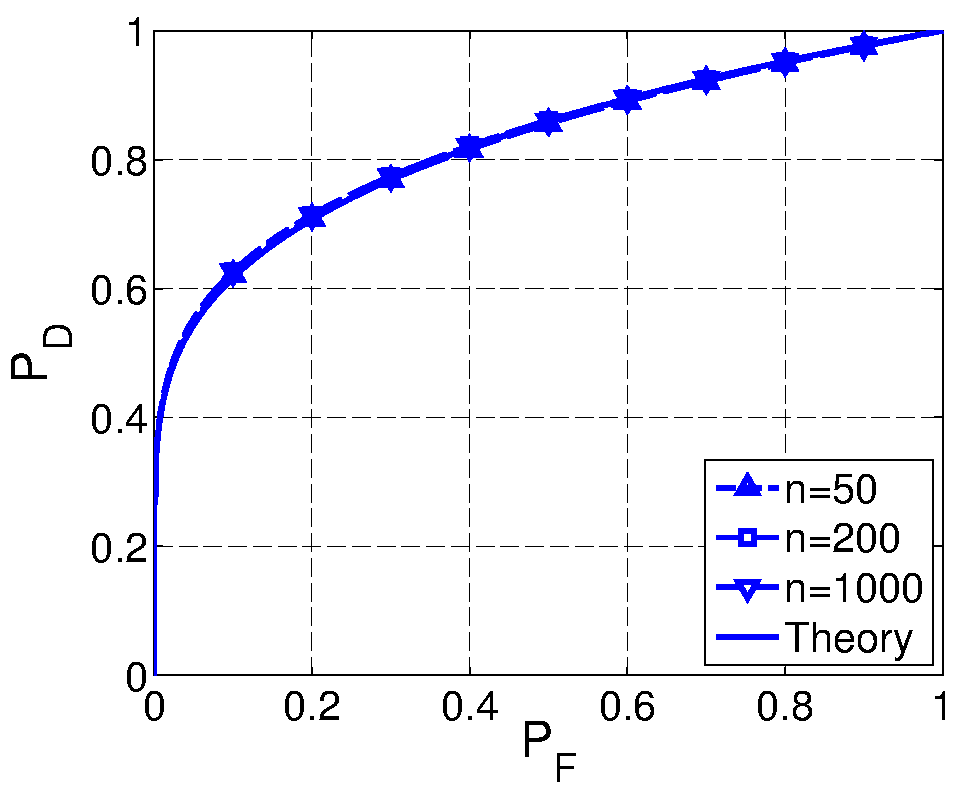
\includegraphics[width=1.5in]{figures/stoch_n_effect1.pdf}
\label{fig:stoch_n_effect1}
}
%\subfigure[$k=2$, $c=10$]{
%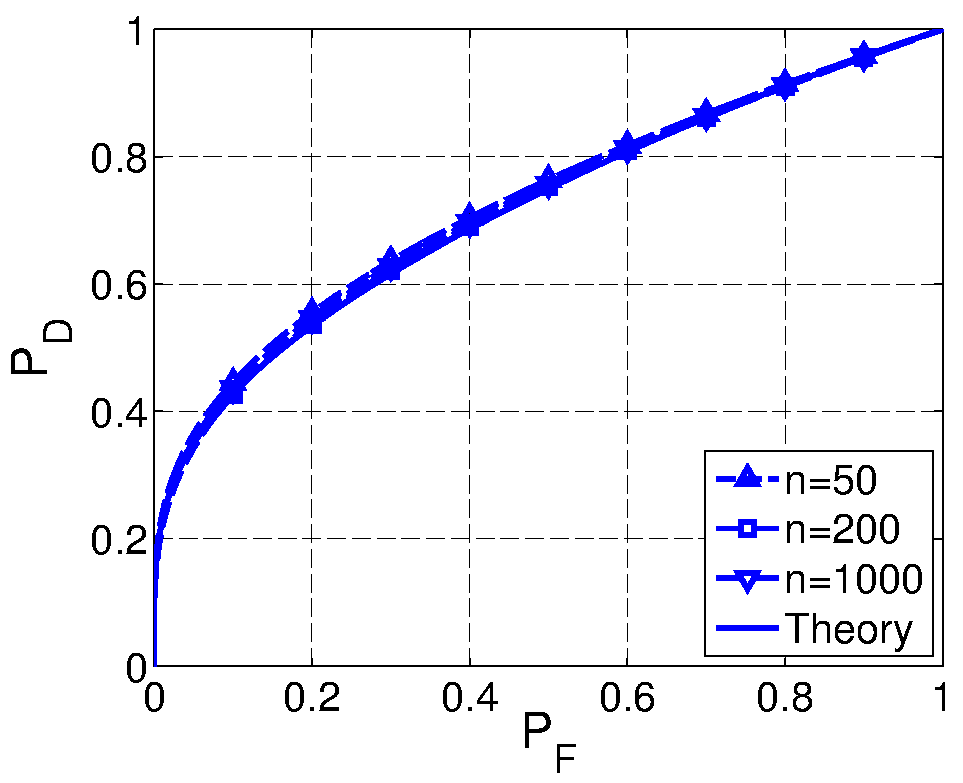
\includegraphics[width=3in]{figures/stoch_n_effect2.pdf}
%\label{fig:stoch_n_effect2}
%}
%\subfigure[$k=4$, $c=1$]{
%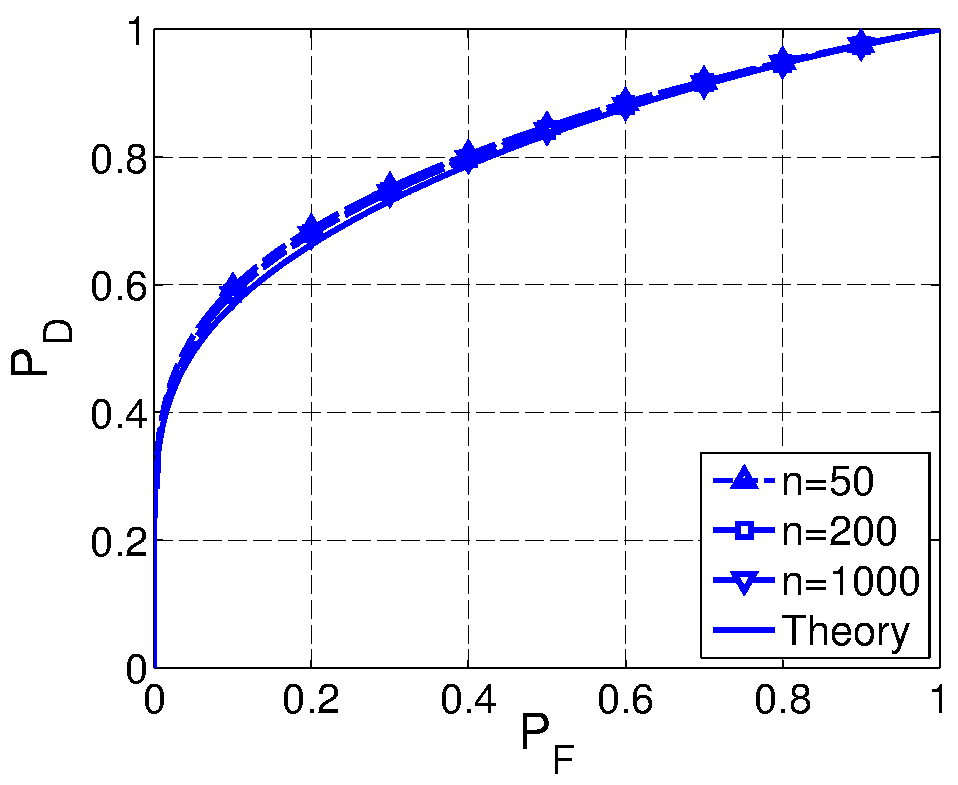
\includegraphics[width=3in]{figures/stoch_n_effect3.pdf}
%\label{fig:stoch_n_effect3}
%}
\subfigure[$k=4$, $c=10$]{
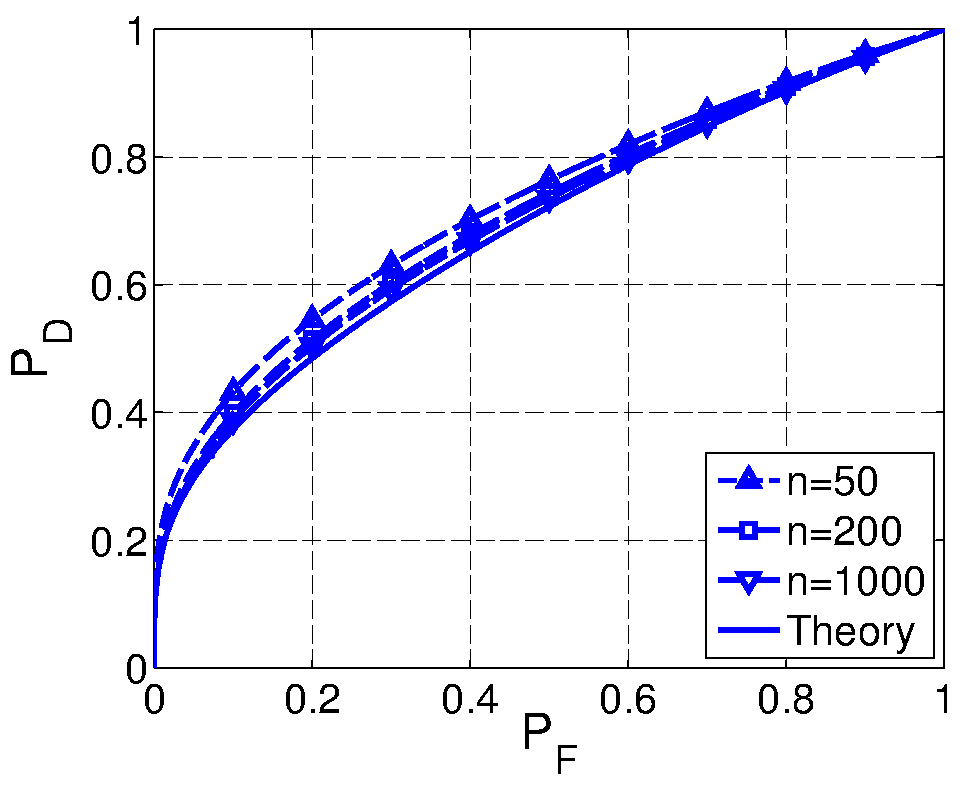
\includegraphics[width=1.5in]{figures/stoch_n_effect4.pdf}
\label{fig:stoch_n_effect4}
}
\vspace{-0.1in}
\caption{Empirical and theoretical ROC curves for the stochastic plug-in detector. Empirical ROC curves were simulated using $10000$ test samples and averaged over 50 trials using algorithms 2 and 4 of \cite{fawcett2006introduction}. (a) $\Sigma=\diag(10,2)$, $c=1$, $\widehat{k}=k=2$ so that $\keff=2$. (b) $\Sigma=\diag(10,2,0.5,0.1)$, $c=10$, $\widehat{k}=k=4$ so that $\keff=1$. Each figure plots empirical ROC curves for $n=50,200,1000$. Theoretical ROC curves were computed as described in Section \ref{sec:roc_theory}. As $n$ increases, the empirical ROC curves approach the theoretically predicted one. However, this convergence is slower for larger $k$ and $c$.}
\vspace{-0.3in}
\end{figure}

\textcolor{blue}{The theoretical ROC curve predictions for the plug-in and RMT detectors rely on the asymptotic approximations that ignore finite $n$ and $m$ correction terms. To examine the validity of the asymptotic approximations (Propositions \ref{th:angles} and \ref{th:eigvals_rmt}, Theorem \ref{th:other angles}, and Corollary \ref{corr:matrix}) and the rate of convergence, we consider two different settings for the stochastic plug-in detector. Figures \ref{fig:stoch_n_effect1}-\ref{fig:stoch_n_effect4} plot three empirical ROC curves for $n=50,200,1000$ as well as the theoretically predicted plug-in ROC curve. Each figure uses different values of $k$ and $c$ but in each case, $\widehat{k}=k$.}

\textcolor{blue}{For both figures, as $n$ increases, the empirical ROC curves approach the theoretical prediction, attesting to the asymptotic convergence of the RMT approximations. Analyzing the rate of convergence (which we conjecture to be $n^{1/2}$ for fixed $k$ and $c$) is an important open problem that we shall tackle in future work. As evident in Figures \ref{fig:stoch_n_effect1}-\ref{fig:stoch_n_effect4} the values of $k$ and $c$ play an important roll in the convergence of the empirical ROC curves. For the larger value of $k$ and $c$ (corresponding to the sample starved regime where the amount of training data is smaller than the system dimensionality i.e. $n>m$) the convergence is also slower. We see that for larger $k$ and $c$, when $n$ is small the empirical ROC curve is not well approximated by the asymptotic theoretical predictions. However, as $n$ increases, the deviation of the empircally generated ROC curve from the theoretically predicted one decreases. Claim \ref{th:other angles} suggests that the off diagonal terms of $\widehat{U}^HU$ asymptotically tend to zero. However, in the finite $n$ and $m$ case these terms are $O(1/\sqrt{n})$ and thus not identically zero. For larger rank systems (increased $k$), there are more of these non-identically-zero terms that worsen the approximation quality for fixed, relatively small $n$. As $n$ increases, this bias vanishes.}

\begin{figure}
\centering
\subfigure[Stochastic]{
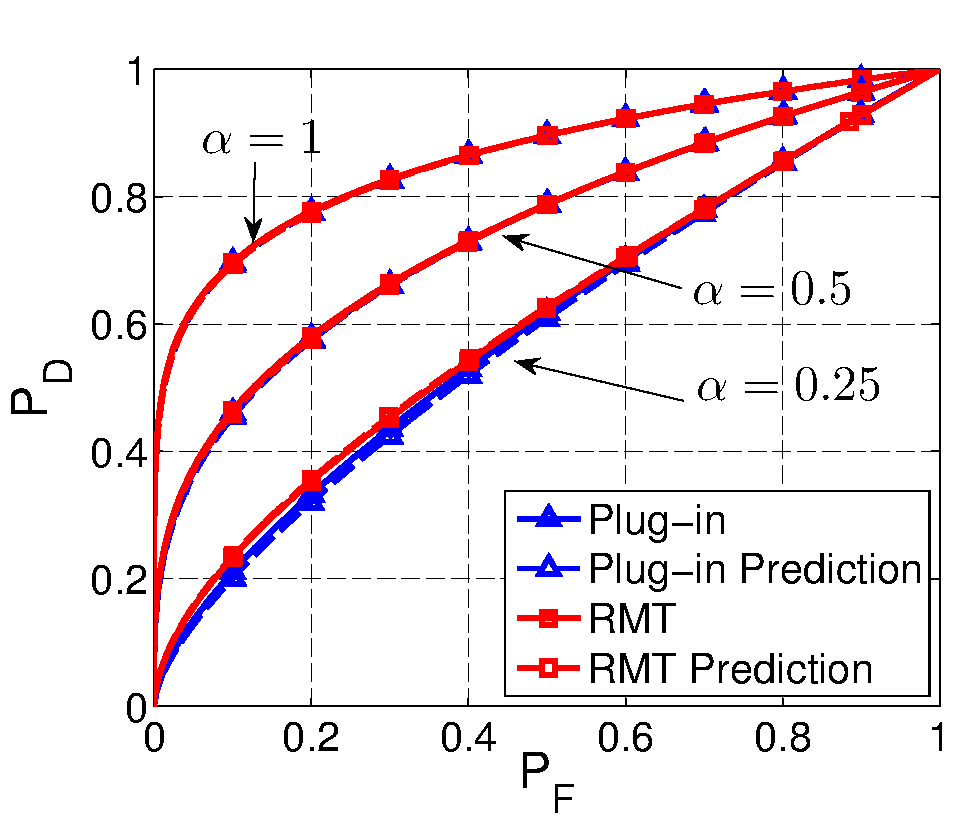
\includegraphics[width=1.5in]{figures/stoch_roc_pred.pdf}
\label{fig:stoch_roc_pred}
}
\subfigure[Deterministic]{
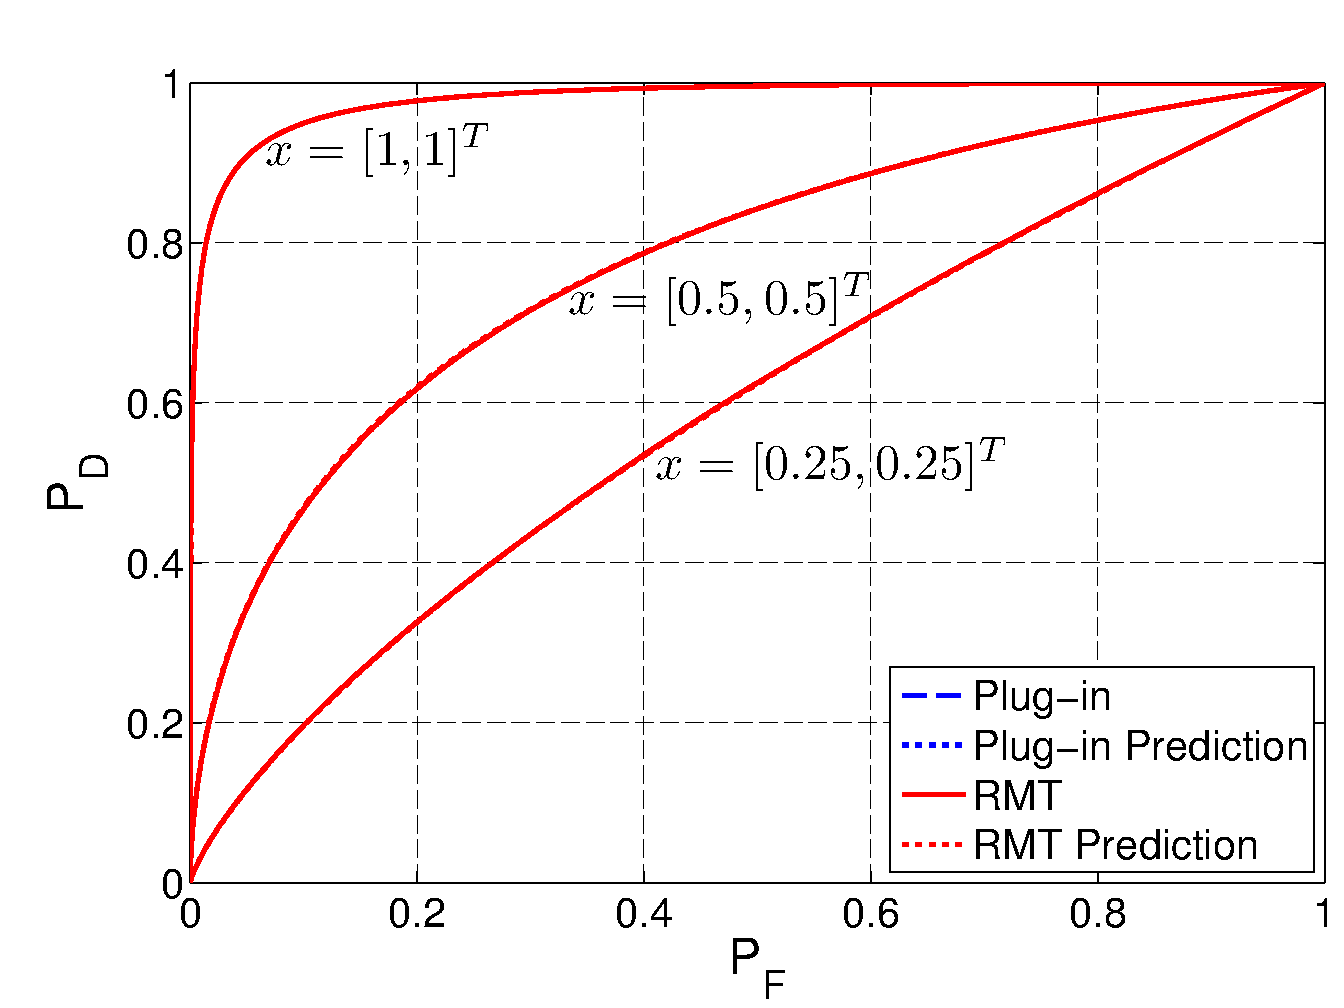
\includegraphics[width=1.5in]{figures/determ_roc_pred.pdf}
\label{fig:determ_roc_pred}
}
\vspace{-0.1in}
\caption{Empirical and theoretical ROC curves for the plug-in and RMT detectors. Empirical ROC curves were simulated using $10000$ test vectors and averaged over 100 trials with $n=1000$, $m=500$, and $\Sigma =\alpha\diag\left(10,5\right)$. The theoretical ROC curves were computed as described in Section \ref{sec:roc_theory}. (a) Stochastic testing seting. Results are plotted for $\alpha=1,0.5,0.25$. For $\alpha=1$ and $\alpha=0.5$, $\widehat{k}=k=k_\text{eff}=2$ by (\ref{eq:keff}). For $\alpha=0.25$, $k_\text{eff}=1$.Since $\widehat{k} > k_{\text{eff}}$ when $\alpha=0.25$, we observe a performance gain when using the RMT detector. (b) Deterministic testing setting. Results are plotted for $\alpha=1$ so that $\keff=2$. Three values of the deterministic signal vector were used: $x=[1,1]^T$, $x=[0.5,0.5]^T$, and $x=[0.25,0.25]^T$. The resulting ROC curves depend on the choice of $x$, however, since $\widehat{k} = k_{\text{eff}}$, the plug-in and RMT detector achieve the same performance for all $x$. For both the stochastic and deterministic detectors, the theoretically predicted ROC curves match the emprical ROC curves, reflecting the accuracy of Corollary \ref{corr:matrix} and the Lugannani-Rice formula.}
\vspace{-0.3in}
\end{figure}

The ROC predictions developed in Section \ref{sec:roc_theory} also depend on parameters such as $\Sigma$ and the deterministic vector $x$. To test the accuracy of the ROC predictions with respect to these parameters, we consider a setting where $\widehat{k}=k = 2$. Figure \ref{fig:stoch_roc_pred} plots empirical and theoretical ROC curves for the plug-in and RMT stochastic detectors for $\Sigma=\alpha\diag(10,5)$ for three choices of $\alpha$. As intuition suggests, smaller values of $\Sigma$ decrease the performance for both the plug-in and RMT detectors. For each choice of $\alpha$, the empirical ROC curves match the ROC predictions that rely on random matrix theoretic approximations presented in Section \ref{sec:rmt}. Using $\alpha=1$ or $\alpha=0.5$ results in $\keff=k=\widehat{k}=2$ but using $\alpha=0.25$ results in $k_\text{eff}=1$. As $\widehat{k}>k_\text{eff}$ for this last case, the plug-in detector realizes a performance loss compared to the RMT detector.

In the deterministic setting, $x$ is an additional parameter that affects detector performance. Figure \ref{fig:determ_roc_pred} plots empirical and theoretical ROC curves for the plug-in and RMT deterministic detectors for $\Sigma=\diag(10,5)$ for three choices of the deterministic test vector $x$. Larger values of $|x|$ result in better detector performance but for each choice of $x$, the theoretically predicted ROC curves match their empirical counterparts. As $x$ does not affect the value of $k_\text{eff}=\widehat{k}=k=2$, the plug-in and RMT detectors achieve the same performance because they have identical statistics. For both test vector models, the theoretical ROC curves match the empirical ROC curves thereby validating the accuracy of the random matrix theoretic approximations employed and the accuracy of the saddlepoint approximation to the c.d.f. used in the stochastic derivation. 

\subsection{Effect of the Number of Training Samples}

\begin{figure}
\centering
\subfigure[$m=5000$]{
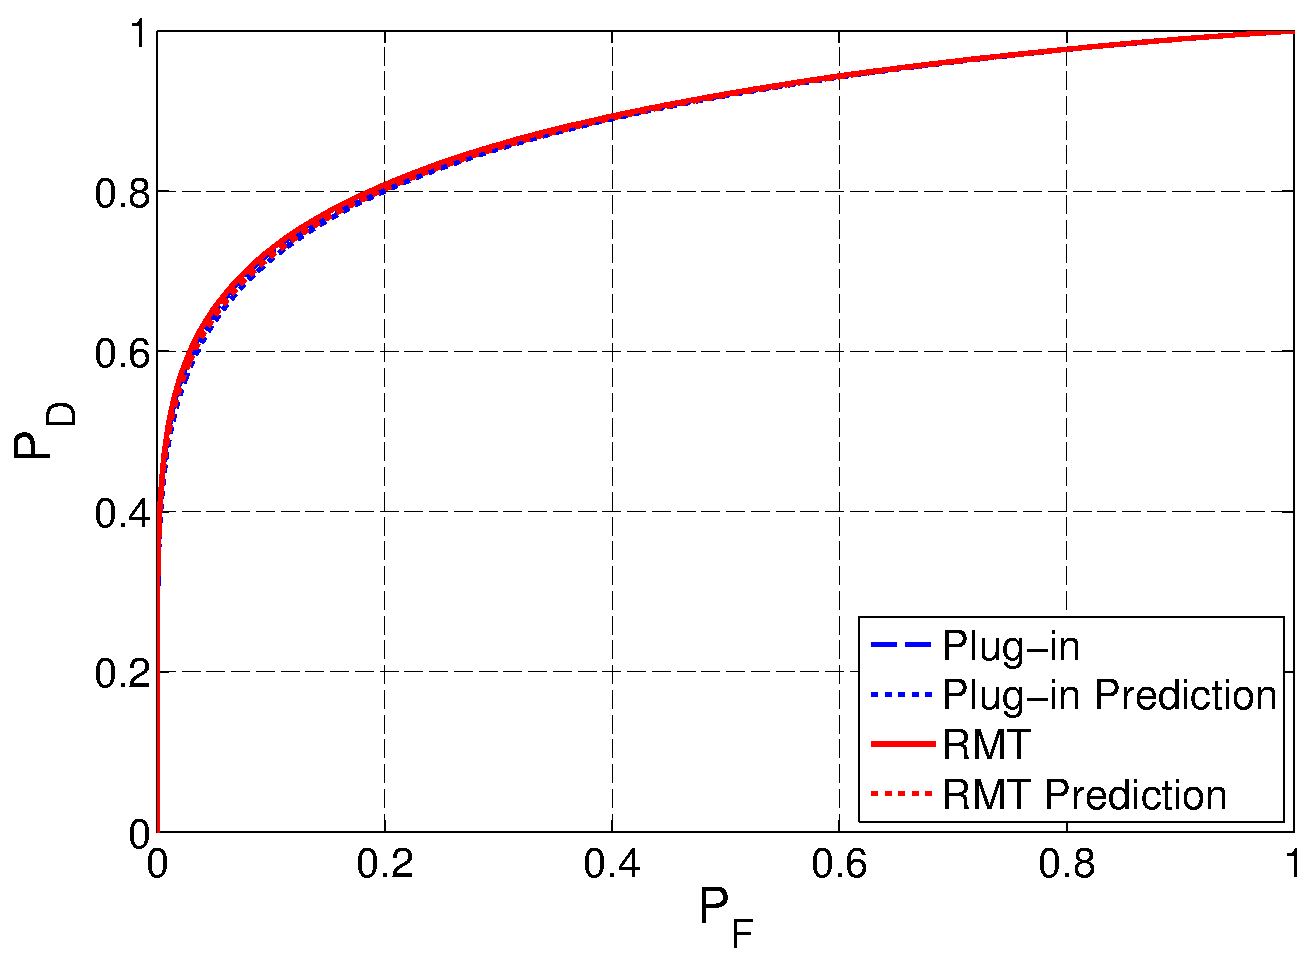
\includegraphics[width=1.5in]{figures/stoch_m_large.pdf}
\label{fig:stoch_m_large}
}
\subfigure[$m=250$]{
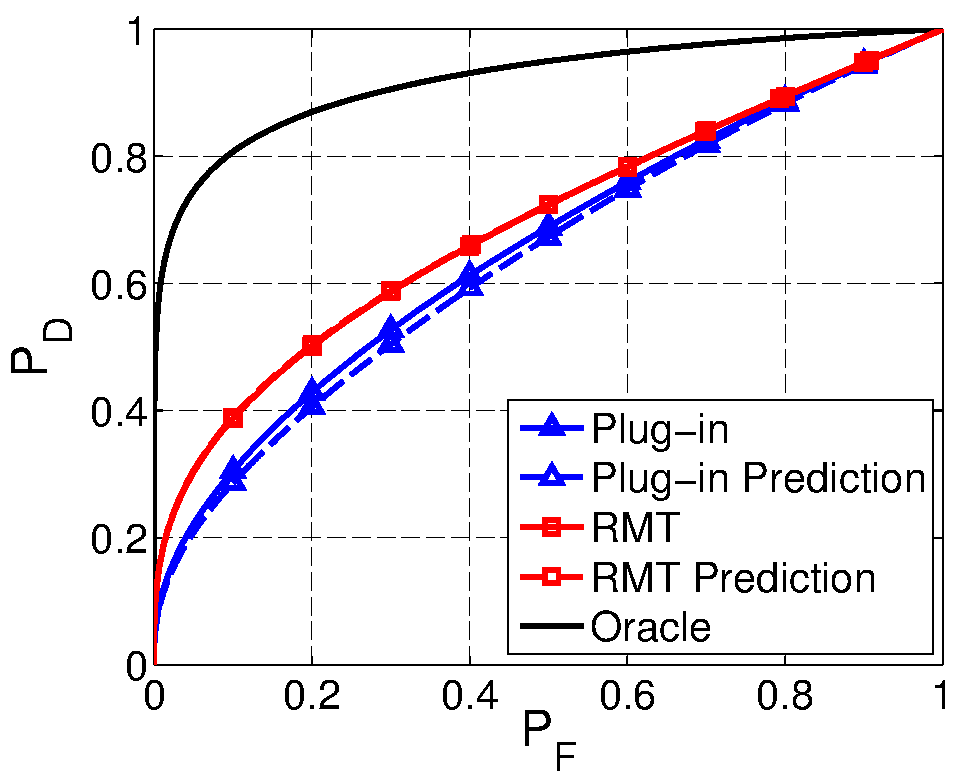
\includegraphics[width=1.5in]{figures/stoch_m_small.pdf}
\label{fig:stoch_m_small}
}
\vspace{-0.1in}
\caption{Empirical and theoretical ROC curves for the plug-in and RMT stochastic detectors. Empirical ROC curves were computed with 10000 test samples and averaged over 100 trials. Here, $n=5000$, $\widehat{k}=k=4$ and $\Sigma = \diag({\bf{10,3,2.5,2}})$. The empirical oracle ROC curve is provided for relative comparison purposes. (a) $m=5000$ so that $c=1$ and $k_\text{eff}=\widehat{k}=4$. The plug-in and RMT detectors achieve relatively the same performance. (b) $m=250$ so that $c=20$ and $\keff=1<\widehat{k}=4$. The RMT detector avoids some of the performance loss realized by the plug-in detector. As seen in Section \ref{sec:std_detecs}, limited training samples degrades detector performance. However, the new RMT detector does not suffer as badly as the plug-in detector because it accounts for subspace estimation errors due to finite training data. The disagreement between the theoretical and empirical ROC curves is attributed to finite dimensionality.}
\label{fig:stoch_m_effect}
\vspace{-0.3in}
\end{figure}

\textcolor{blue}{We saw in Section \ref{sec:training_effect} that finite training data degraded the performance of the plug-in detector relative to that of the oracle detector. The analysis of Section \ref{sec:rmt} mathematically justifies this observation showing that, for a fixed $\Sigma$, the number of training samples, $m$, directly affects $k_\text{eff}$ via (\ref{eq:keff}). While the plug-in detector ignores this analysis, we derived a new RMT detector that accounts for subspace estimation errors due to finite training data. By only using the $\keff$ informative signal subspace components, we hope that the RMT detector will avoid some of the performance loss associated with the plug-in detector. To explore how the number of training samples affects the relative performances of the plug-in and RMT detectors, we first consider the setting where $\widehat{k}=k=4$ with $\Sigma=\diag(10,3,2.5,2)$. }

Figures \ref{fig:stoch_m_large} and \ref{fig:determ_m_large} investigate the performance when $m=n$ so that $c=1$ for the stochastic and deterministic settings, respectively. This choice of $m$ results in $k_\text{eff}=\widehat{k}=4$. As expected, for both settings the plug-in and RMT detectors achieve relatively the same performance because $\widehat{k}=\keff$. Figures \ref{fig:stoch_m_small} and \ref{fig:determ_m_small} choose $20m=n$ so that $c=20$ and $k_\text{eff}=1$ for the stochastic and deterministic settings, respectively. This corresponds to the sample starved regime where $m<n$. In this second experiment, the plug-in detectors becomes suboptimal for both testing settings because they use $4=\widehat{k} > k_\text{eff}=1$ subspace components. Whenever $k_\text{eff}<\widehat{k}$ the RMT detectors avoid some of the performance loss (compared to the oracle detectors) realized by the plug-in detectors. We could have observed this same effect by instead varying $\Sigma$ as both of these quantities drive the value of $k_\text{eff}$. The disagreement between the theoretical and empirical stochastic ROC curves for the plug-in detector is attributed to the finite $n$ and $m$ correction terms, which we have discussed previously.

\textcolor{blue}{Figures \ref{fig:stoch_m_effect} and \ref{fig:determ_m_effect} show that the number of training samples helps to drive the performance of matched subspace detectors. In Section \ref{sec:std_detecs}, we mathematically defined the performance loss of a detector relative to its oracle detector as $\epsilon$ in (\ref{eq:epsilon}) and empirically plotted the number of training samples needed to achieve a desired performance loss for the stochastic plug-in detector in Figure \ref{fig:epsilon_graph}. Figures \ref{fig:stoch_theory_epsilon} and \ref{fig:determ_theory_epsilon} theoretically plot this same curve for the plug-in and RMT detectors for each testing setting, respectively.}

\textcolor{blue}{These figures show that when $\keff<\widehat{k}$, the RMT detector achieves a much smaller performance loss for a fixed number of training samples. Put another way, to achieve the same performance loss, the RMT detectors need a significantly less number of training samples when $\keff<\widehat{k}$. Figure \ref{fig:stoch_theory_epsilon} shows that the stochastic detectors can acheive an arbitrarily small performance loss given a particularly large number of training samples. However, Figure \ref{fig:determ_theory_epsilon} shows that there is a performance loss limit for the deterministic detectors and that this limit may be different for the RMT and plug-in detectors. As discussed in Section \ref{sec:std_detecs}, this arises because the oracle deterministic detector assumes that $x$ is known. As $m\to\infty$, $\widehat{U}\to U$ and $\widehat{\Sigma}\to\Sigma$, however, the plug-in detector's estimate of $\widehat{x}$ still depends on the noisy observed data $y$. Therefore, unlike the stochastic detectors that can achieve an arbitrarily small performance loss, the deterministic plug-in and RMT detectors can never achieve the same performance as the deterministic oracle detector.}

\begin{figure}
\centering
\subfigure[$m=5000$]{
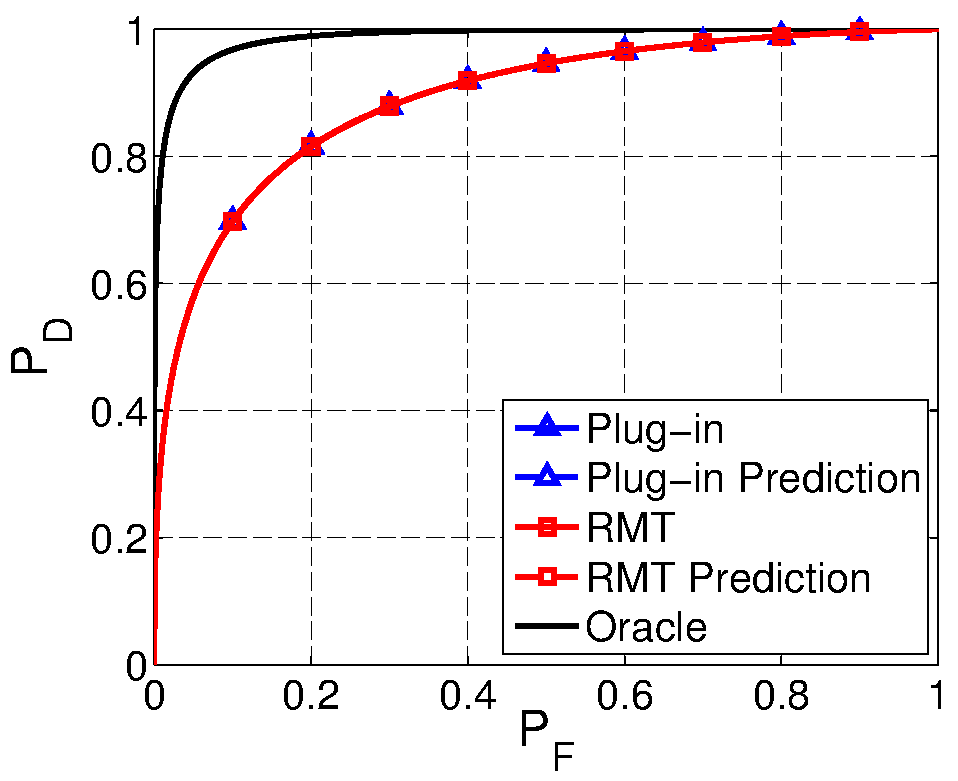
\includegraphics[width=1.5in]{figures/determ_m_large.pdf}
\label{fig:determ_m_large}
}
\subfigure[$m=250$]{
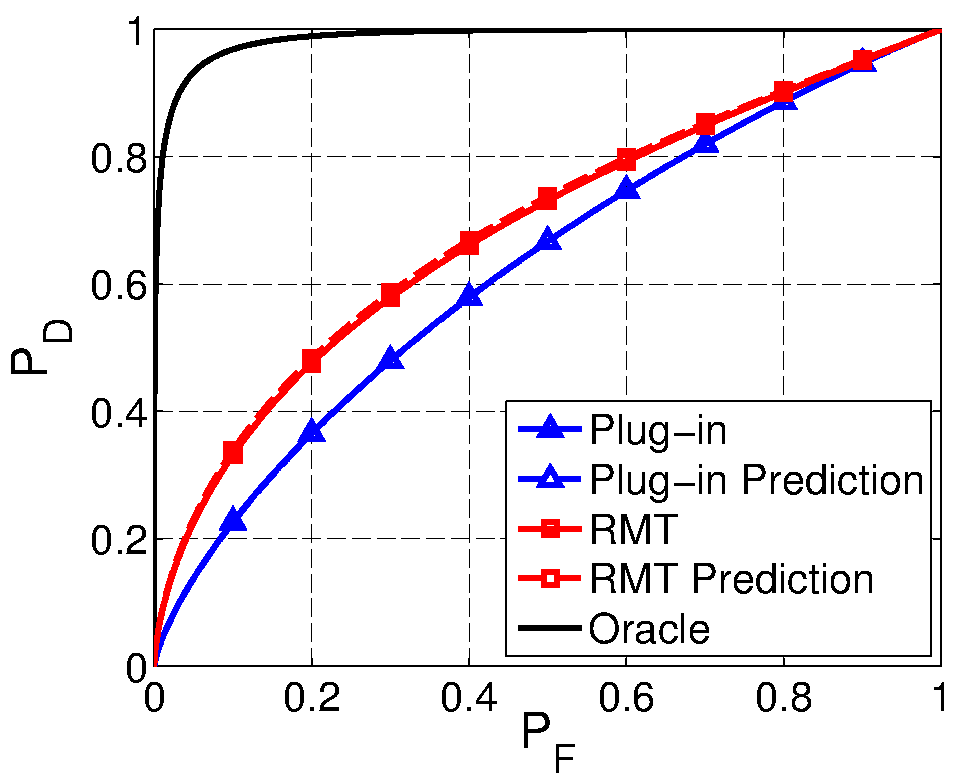
\includegraphics[width=1.5in]{figures/determ_m_small.pdf}
\label{fig:determ_m_small}
}
\vspace{-0.1in}
\caption{Analagous figures to Figures \ref{fig:stoch_m_large} and \ref{fig:stoch_m_small} for the deterministic detectors when $x=0.75\times[1,1,1,1]^T$. When $\keff<\widehat{k}$ we see that the RMT detector avoids some of the performance loss of the plug-in detector due to finite training data.}
\label{fig:determ_m_effect}
\vspace{-0.2in}
\end{figure}

\begin{figure}
\centering
\subfigure[Stochastic]{
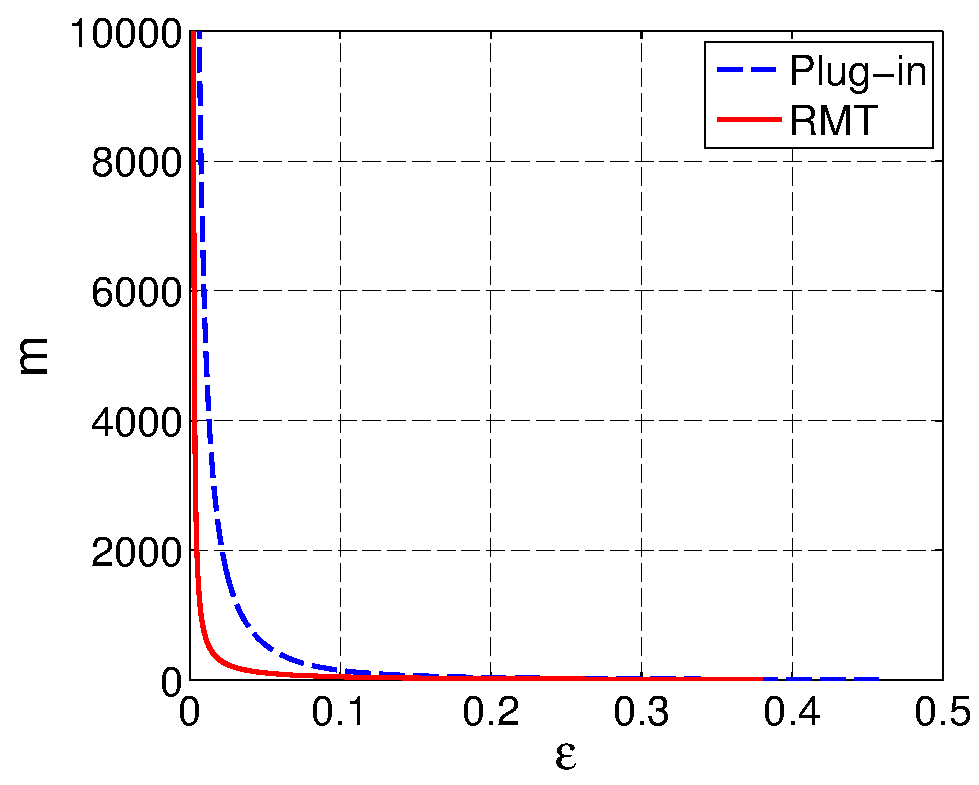
\includegraphics[width=1.5in]{figures/stoch_theory_epsilon_graph.pdf}
\label{fig:stoch_theory_epsilon}
}
\subfigure[Deterministic]{
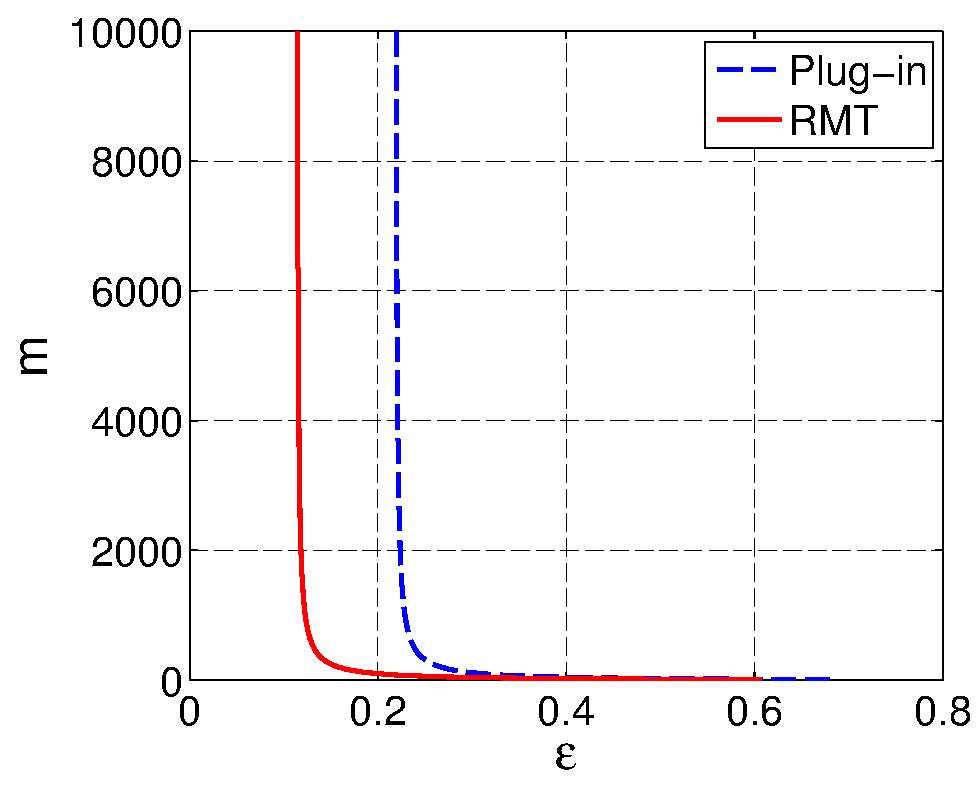
\includegraphics[width=1.5in]{figures/determ_theory_epsilon_graph.pdf}
\label{fig:determ_theory_epsilon}
}
\vspace{-0.1in}
\caption{Theoretically determined number of training samples, $m$, needed to achieve a desired performance loss, $\epsilon$, as defined in (\ref{eq:epsilon}). The required false alarm rate is $P_F=0.1$ with $n=200$, $\Sigma = \diag(10,0.1)$, and $\widehat{k}=k=2$. (a) Results for the stochastic detectors. We see that for a given $\epsilon$, the new RMT detector requires less training samples. (b) Results for the deterministic detectors when $x=[0.75,0.75]^T$. Again, for a given $\epsilon$, the new RMT detector requires less training samples. In the deterministic setting, the limiting performance loss is different (and non-zero) for the plug-in and RMT detectors. This arises in estimation errors of $x$ in the GLRT.}
\label{fig:epsilon_combined}
\end{figure}


%we have neglected. As $k$ increases, there are more off-diagonal terms in the covariance matrix in (\ref{eq:cov mat}) that are not identically zero, as discussed earlier. Theorem \ref{th:other angles} shows that asymptotically these off diagonal terms decay to zero but in the finite $n$ and $m$ case, they are non-zero. In the case of larger $k$, there are more of these non-identically-zero terms thereby worsening the approximation.

\subsection{Effect of $\widehat{k}$}
\begin{figure}
\centering
\subfigure[Stochastic]{
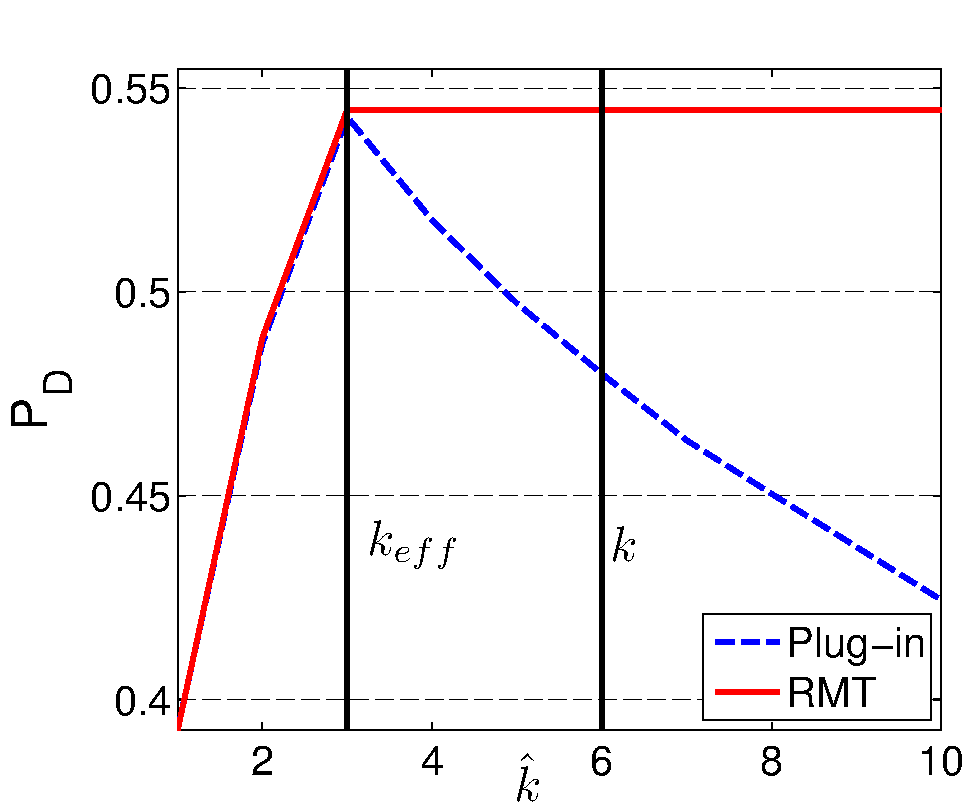
\includegraphics[width=1.5in]{figures/stoch_khat_graph.pdf}
\label{fig:stoch_khat}
}
\subfigure[Deterministic]{
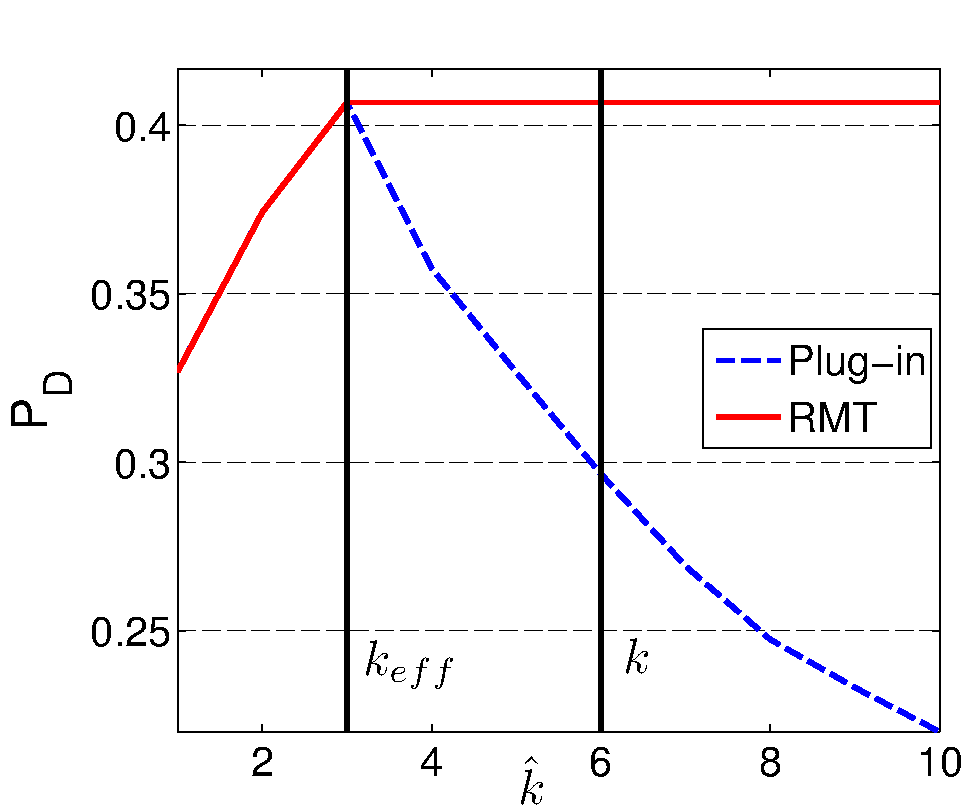
\includegraphics[width=1.5in]{figures/determ_khat_graph.pdf}
\label{fig:determ_khat}
}
\vspace{-0.1in}
\caption{Empirical exploration of the achieved probability of detection, $P_D$, for a fixed probability of false alarm, $P_F=0.01$, for various $\widehat{k}$. Empirical ROC curves were computed using 10000 test samples and averaged over 100 trials with $n=1000$, $m=500$, and $\Sigma = \diag({\bf{10,5,4}},0.75,0.5,0.25)$ so that $k_{\text{eff}}=3$. (a) Results for the stochastic detectors. (b) Results for the deterministic detecotrs using $x=0.75\times[1,1,1,1,1,1]^T$. In both test settings, the optimal $\widehat{k}$ resulting in the largest $P_D$ is not the true $k$, but rather $k_\text{eff}$.}
\label{fig:khat_graphs}
\vspace{-0.3in}
\end{figure}

\textcolor{blue}{We discussed in Section \ref{sec:param_estim} that we are given a dimension estimate $\widehat{k}$ when deriving our detector. From our perspective, we don't know how $\widehat{k}$ was estimated (possibly from the training data or by a domain expert) but simply use it when forming our subpsace and signal covariance estimates.} Figures \ref{fig:stoch_khat} and \ref{fig:determ_khat} empirically examine the performance of the plug-in and RMT detectors as a function of $\widehat{k}$ for the stochastic and deterministic test settings, respectively. Here, we relax the constraint that $\widehat{k}\geq k$. The figures plot the achieved probability of detection for a constant false alarm rate of $0.01$. The result confirms that, for both settings, $k_\text{eff}$ is the optimal choice for $\widehat{k}$. When the plug-in detectors use $\widehat{k} = k_\text{eff}$ they achieve an equivalent performance as that of the RMT detector.

Setting $\widehat{k} < \keff$ drastically degrades performance for all detectors. In this regime, the plug-in and RMT detectors realize the same ROC performance, demonstrating that quantification and exploitation of the subspace estimation accuracy ($|\langle u_i,\widehat{u}_i\rangle |^2_{\text{rmt}}$ and $\sigma_{i_\text{rmt}}^2$), while useful in ROC performance prediction, does \textit{not} noticeably enhance detection performance. When $\widehat{k} > k_\text{eff}$, the performances of the plug-in detectors degrade while those of the RMT detectors are stable as if $\widehat{k}=k_\text{eff}$. In other words, we do not pay a price for overestimating the subspace dimension with the RMT detectors. This makes sense (and is slightly contrived) because the RMT detectors will only sum to a maximum of $k_\text{eff}$ indices as evident in (\ref{eq:optimal_stat_stoch}) and (\ref{eq:optimal_stat_determ}). In many applications, practitioners might employ the ``play-it-safe'' approach and set $\widehat{k}$ to be significantly greater than $k_\text{eff}$. The performance loss caused by adding each uninformative subspace, as seen in Figure \ref{fig:khat_graphs}, constitutes evidence to the assertion that overestimating the signal subspace dimension is a bad idea. When $k_\text{eff} < k$, even perfectly estimating the subspace dimension (i.e. setting $\widehat{k} = k$) is suboptimal.


\section{Conclusion}\label{sec:conclusion}
In this paper, we considered a matched subspace detection problem where the low-rank signal subspace is unknown and must be estimated from finite, noisy, signal-bearing training data. We considered both a stochastic and deterministic model for the testing data. The subspace estimate is inaccurate due to finite and noisy training samples and therefore degrades the performance of plug-in detectors compared to an oracle detector. We showed how the ROC performance curve can be derived from the RMT-aided quantification of the subspace estimation accuracy.

Armed with this RMT knowledge, we derived a new RMT detector that only uses the effective number of informative subspace components, $k_\text{eff}$. Plug-in detectors that use the uninformative components will thus incur a performance degradation, relative to the RMT detector. \textcolor{blue}{In settings where a practitioner might play-it-safe and set $\widehat{k}> \widehat{k}_{\text{eff}}$, the performance loss in significant (see Figures \ref{fig:stoch_theory_epsilon} and \ref{fig:determ_theory_epsilon} for a demonstration of how much training data such a play-it-safe plug-in detector would need to match the performance of a $\keff$-tuned RMT detector).} This highlights the importance of robust techniques \cite{nadakuditi2010fundamental,johnstone2001distribution,el2007tracy} for estimating $k_\text{eff}$ in subspace based detection schemes as opposed to estimating $k$, particularly in the regime where $k_{\text{eff}} < k$.  We showed in Tables \ref{table:summary_stoch} and \ref{table:summary_determ} that the distributions of the test statistics could be expressed as a weighted sum of independent chi-squared random variables. The associated ROC curves can then be computed using a saddlepoint approximation.

\textcolor{blue}{The results in this paper can be extended in several directions. We note that the stochastic detector setting assumed normally distributed training and test data. We can extend the analysis to the Gaussian training data but non-Gaussian test vector setting by `integrating-out' the deterministic detector performance curves with respect to the non-Gaussian distribution of the test-vector. Our results relied on characterization of the quantity $\langle u_{j},\widehat{u}_{i}\rangle$.  Thus analogous performance curves can be obtained for any alternate training data models for which this quantity can be analytically quantified. To that end, the results in \cite{benaych2011singular} facilitate such an analysis for a broader class of models including the correlatted Gaussians training data setting. An extension to the missing data setting might follow a similar approach and appears within reach. Aspects related to rate of convergence are open and will be the subject of future work.}



\section*{Appendix}
\textit{Theorem 5.1:} Assume the same hypothesis as in Proposition \ref{th:angles}. Let $\widehat{k}=\keff=k$. For $i=1,\dots,\widehat{k}$, $j=1,\dots,k$, and $i\neq j$, as $n,m\to\infty$ with $n/m\to c$, then $\langle u_j,\widehat{u}_i\rangle \convas 0.$
\begin{proof}
Let $U_{n,k}$ be a $n\times k$ real or complex matrix with orthonormal columns, $u_i$ for $1\leq i\leq k$. Let $\Sigma = \diag\left(\sigma_1^2,\dots,\sigma_k^2\right)$ such that $\sigma_1^2>\sigma_2^2>\dots>\sigma_k^2>0$ for $k\geq 1$. Define $P_n=U_{n,k}\Sigma U_{n,k}^H$ so that $P_n$ is rank-$k$. Let $Z_n$ be a $n\times m$ real or complex matrix with independent $\mathcal{CN}\left(0,1\right)$ entries. Let $X_n=\frac{1}{m}Z_nZ_n^H$, which is a random Wishart matrix, have eigenvalues $\lambda_1(X_n)\geq\dots\geq\lambda_n(X_n)$. Let $\widehat{X}_n=X_n\left(I_n+P_n\right)$. $X_n$ and $P_n$ are independent by assumption. Define the empirical eigenvalue distribution as $\mu_{X_n}=\frac{1}{n}\sum_{j=1}^n\delta_{\lambda_j\left(X_n\right)}$. We assume that as $n\to\infty$, $\mu_{X_n}\overset{\text{a.s.}}{\longrightarrow}\mu_X$.


For $i=1,\dots, \widehat{k}=k$, let $\widehat{v}_i$ be an arbitrary unit eigenvector of $\widehat{X}_n$. By the eigenvalue master equation, $\widehat{X}_n\widehat{v}_i=\widehat{\lambda}_i\widehat{v}_i$, it follows that
\begin{equation}\label{eq:eval_master}
\begin{aligned}
  &U_{n,k}^H\left(\widehat{\lambda}_iI_n-X_n\right)^{-1}X_nU_{n,k}\Sigma U_{n,k}^H\widehat{v}_i&&=U_{n,k}^H\widehat{v}_i.\\
\end{aligned}
\end{equation}
Let $X_n=V_n\Lambda_nV_n^H$ be the eigenvalue decomposition of $X_n$ such that $\Lambda_n=\diag(\lambda_1(X_n),\dots,\lambda_n(X_n))$ and $\lambda_1(X_n)\geq\dots\geq\lambda_n(X_n)$. Using this decomposition and defining $W_{n,k}=V^HU_{n,k}$, (\ref{eq:eval_master}) simplifies to
\begin{equation}\label{eq:eval_master2}
\begin{aligned}
  &W_{n,k}^H\left(\widehat{\lambda}_iI_n-\Lambda_n\right)^{-1}\Lambda_nW_{n,k}\Sigma U_{n,k}^H\widehat{v}_i&&=U_{n,k}^H\widehat{v}_i.\\
\end{aligned}
\end{equation}
Define the columns of $W_{n,k}$ to be $w_j^{(n)}=[w_{1,j}^{(n)},\dots,w_{n,j}^{(n)}]^T$ for $j=1,\dots,k$. These columns are orthonormal and isotropically random. We can rewrite (\ref{eq:eval_master2}) as
\begin{equation}\label{eq:t_trans}
\left[T_{\mu_{r,j}^{\left(n\right)}}\left(\widehat{\lambda}_i\right)\right]_{r,j=1}^k \Sigma U_{n,k}^H\widehat{v}_i=U_{n,k}^H\widehat{v}_i
\end{equation}
where for $r=1,\dots,k$, $j=1,\dots,k$, $\mu_{r,j}^{\left(n\right)}=\sum_{\ell=1}^n\overline{w_{\ell,r}^{\left(n\right)}}w_{\ell,j}^{\left(n\right)}\delta_{\lambda_\ell\left(X_n\right)}$ is a complex measure and $T_{\mu_{r,j}^{\left(n\right)}}$ is the T-transform defined by $T_{\mu}\left(z\right) = \int\frac{t}{z-t}d\mu\left(t\right)\,\,\,\,\text{for } z\not\in\text{supp } \mu$. We may rewrite (\ref{eq:t_trans}) as
\begin{equation*}
\left(I_k-\left[\sigma_j^2T_{\mu_{r,j}^{\left(n\right)}}\left(\widehat{\lambda}_i\right)\right]_{r,j=1}^k\right)U_{n,k}^H\widehat{v}_i=0.
\end{equation*}
Therefore, $U_{n,k}^H\widehat{v}_i$ must be in the kernel of $M_n\left(\widehat{\lambda}_i\right)=I_k-\left[\sigma_j^2T_{\mu_{r,j}^{\left(n\right)}}\left(\widehat{\lambda}_i\right)\right]_{r,j=1}^k$.
By Proposition 9.3 of \cite{benaych2011eigenvalues}
\begin{equation*}
\mu_{r,j}^{\left(n\right)}\overset{\text{a.s.}}{\longrightarrow}\begin{cases}\mu_X & \text{for } i=j \\ \delta_0 & \text{o.w.} \end{cases}
\end{equation*}
where $\mu_X$ is the limiting eigenvalue distribution of $X_n$. Therefore,
\begin{equation*}
M_n\left(\widehat{\lambda}_i\right)\overset{\text{a.s.}}{\longrightarrow}\diag\left(1-\sigma_1^2T_{\mu_X}\left(\widehat{\lambda}_i\right), \dots, 1-\sigma_k^2T_{\mu_X}\left(\widehat{\lambda}_i\right)\right).
\end{equation*}
As $k_\text{eff}=k$, for $i=1,\dots,k$, $\sigma_i^2>1/T_{\mu_X}(b^+)$, where $b$ is the supremum of the support of $\mu_X$. As $\widehat{\lambda}_i$ is the eigenvalue corresponding to the eigenvector $\widehat{v}_i$, by Theorem 2.6 of \cite{benaych2011eigenvalues} $\widehat{\lambda}_i\overset{\text{a.s.}}{\longrightarrow}T^{-1}_{\mu_X}\left(1/\sigma_i^2\right)$. Therefore,
\footnotesize\begin{equation}\label{eq:Mn}
M_n\left(\widehat{\lambda}_i\right)\overset{\text{a.s.}}{\longrightarrow}\diag\left(1-\frac{\sigma_1^2}{\sigma_i^2}, \dots, 1-\frac{\sigma_{i-1}^2}{\sigma_i^2}, 0, 1-\frac{\sigma_{i+1}^2}{\sigma_i^2}, \dots, 1-\frac{\sigma_k^2}{\sigma_i^2}\right)
\end{equation}\normalsize
Recall that $U_{n,k}^H\widehat{v}_i$ must be in the kernel of $M_n\left(\widehat{\lambda}_i\right)$. Therefore, any limit point of $U_{n,k}^H\widehat{v}_i$ is in the kernel of the matrix on the right hand side of (\ref{eq:Mn}). Therefore, for $i\neq j$, $i=1,\dots,\widehat{k}$, $j=1,\dots,k$, we must have that $\left(1-\frac{\sigma_j^2}{\sigma_i^2}\right)\langle u_j,\widehat{v}_i\rangle=0$. As $\sigma_i^2\neq\sigma_j^2$, for this condition to be satisfied we must have that for $j\neq i$, $i=1,\dots,\widehat{k}$, $j=1,\dots,k$, $\langle u_j,\widehat{v}_i\rangle\overset{\text{a.s.}}{\longrightarrow}0$.

Recall that our observed vectors $y_i\in\complex^{n\times 1}$ have covariance matrix $U_{n,k}\Sigma U_{n,k}^H+I_n=P_n+I_n$. Therefore, our observation matrix, $Y_n$ which is a $n\times m$ matrix, may be written $Y_n=\left(P_n+I_n\right)^{1/2}Z_n$. The sample covariance matrix, $S_n=\frac{1}{m}Y_nY_n^H$, may be written $S_n=\left(I_n+P_n\right)^{1/2}X_n\left(I_n+P_n\right)^{1/2}$. By similarity transform, if $\widehat{v}_i$ is a unit-norm eigenvector of $\widehat{X}_n$ then $\widehat{s}_i=\left(I_n+P_n\right)^{1/2}\widehat{v}_i$ is an eigenvector of $S_n$. If $\widehat{u}_i=\widehat{s}_i/\|\widehat{s}_i\|$ is a unit-norm eigenvector of $S_n$, it follows that
\begin{equation*}
\langle u_j,\widehat{u}_i\rangle=\frac{\sqrt{\sigma_i^2+1}\langle u_j,\widehat{v}_i\rangle}{\sqrt{\sigma_i^2|\langle u_j,\widehat{v}_i\rangle|^2+1}}
\end{equation*}
As $\langle u_j,\widehat{v}_i\rangle\overset{\text{a.s.}}{\longrightarrow}0$ for all $i\neq j$, $i=1,\dots,\widehat{k}$, $j=1,\dots,k$, it follows that $\langle u_j,\widehat{u}_i\rangle\overset{\text{a.s.}}{\longrightarrow}0$ for all $i\neq j$ $i=1,\dots,\widehat{k}$, $j=1,\dots,k$.

%%%%%%%%%%%%%%%%%%%%% CLAIM %%%%%%%%%%%%%%%%%%%%%%%%%%%%%%%%%%%%%%%%%%%%%

\textit{Claim 5.1:}  We conjecture that this result holds for the general case of $i\neq
j$, $i=1,\dots,\widehat{k}$, $j=1,\dots,k$, not just when $\widehat{k}=\keff=k$. Consider
the case when $k=1$. For $i>2$, if $\widehat{\lambda}_i$ is an eigenvalue of
$\widehat{X}_n=X_n(I_n+\sigma^2uu^H)$, then it satisfies
$\det(\widehat{\lambda}_iI_n-X_n(I_n+\sigma^2uu^H)) =
\det(\widehat{\lambda}_iI_n-X_n)\det(I_n-(\widehat{\lambda}_iI_n-X_n)^{-1}X_n\sigma^2uu^H)=0$. Therefore,
if $\widehat{\lambda}_i$ is not an eigenvalue of $X_n$, the corresponding unit norm
eigenvector $\widehat{v}_i$ is in the kernel of
$I_n-(\widehat{\lambda}_iI_n-X_n)^{-1}X_n\sigma^2uu^H$. Therefore
\begin{equation*}
  |\langle \widehat{v}_i,u\rangle |^2 = \frac{1}{\sigma^4u^HX_n\left(\widehat{\lambda}_iI_n-X_n\right)^{-2}X_nu}.
\end{equation*}
Recall that Weyl's interlacing lemma for eigenvalues gives $\lambda_i(X_n)\leq
\widehat{\lambda}_i\leq \lambda_{i-1}(X_n)$. Letting $X_n=V_n\Lambda_nV_n^H$ and
$w=V_n^Hu$, we see the importance of the
asymptotic spacing of eigenvalues of $X_n$ in
%\begin{equation*}
%  u^HX_n(\widehat{\lambda}_jI_n-X_n)^{-2}X_nu =\sum_{\ell=1}^n\frac{|w_\ell|^2\lambda_\ell^2(X_n)}{\left(\widehat{\lambda}_j-\lambda_\ell\right)^2}\geq\frac{|w_{j-1}|^2\lambda_{j-1}^2(X_n)}{|\lambda_{j-1}-\lambda_j|^2}+\frac{|w_{j}|^2\lambda_j^2(X_n)}{|\lambda_{j-1}-\lambda_j|^2}.
%\end{equation*}
\begin{equation*}
  u^HX_n(\widehat{\lambda}_iI_n-X_n)^{-2}X_nu
  =\sum_{\ell=1}^n\frac{|w_\ell|^2\lambda_\ell^2(X_n)}{\left(\widehat{\lambda}_i-\lambda_\ell\right)^2}\geq
  \frac{\min_j\lambda_j^2(X_n)\min_j|w_j|^2}{\max_j |\lambda_{j-1}-\lambda_j|^2}
\end{equation*}
%In  \cite{jiang2004limiting} it is shown that $\min_j\lambda_j^2(X_n)=\lambda_n^2(X_n)
%\convas (1-\sqrt{c})^4$. The typical spacing between eigenvalues is $O(1/n)$ while the
%typical magnitude of $w_i^2$ is $O(1/n)$. Therefore, the above inequality will typically be $O(n)$ and we get the desired
%result of $|\langle \widehat{v}_j,u\rangle |^2\convas 0$. More generally, it is the
%behavior of the largest eigenvalue gap and the smallest element of $w_i$ that drives this
%convergence. Thus, so long as the eigenvector whose elements are $w_i$ are delocalized
%(having elements of $O(1/\sqrt{n})$ and the smallest gap between $k$ successive
%eigenvalues is at least as large as $O(1/n + \epsilon)$, we may bound the right hand side
%of the above inequality. The claim follows after applying a similarity transform as in the
%proof of Theorem 5.1.

In \cite{silverstein1985smallest} it is shown that $\min_j\lambda_j^2(X_n)=\lambda_n^2(X_n)
\convas (1-\sqrt{c})^2$. The typical spacing between eigenvalues is $O(1/n)$ while the
typical magnitude of $w_j^2$ is $O(1/n)$ \cite{barvinok2005measure}. Therefore, the right hand side of the above inequality will typically be $O(n)$ and we get the desired
result of $|\langle \widehat{v}_i,u\rangle |^2\convas 0$. More generally, it is the
behavior of the largest eigenvalue gap and the smallest element of $w_i$ that drives this
convergence. Thus, so long as the eigenvector whose elements are $w_i$ are delocalized
(i.e. having elements of $O(1/\sqrt{n})$) and the smallest gap between $k$ successive
eigenvalues is at least as large as $O(1/(n^{(0.5+ \epsilon)})$, the right hand side of the inequality will be unbounded with $n$. The claim follows after applying a similarity transform as in the
proof of Theorem 5.1.


\end{proof}


% use section* for acknowledgement
\section*{Acknowledgment}

This work is supported by the ONR Young Investigator Program under Grant N00014-11-1-0660.


% Can use something like this to put references on a page
% by themselves when using endfloat and the captionsoff option.
\ifCLASSOPTIONcaptionsoff
  \newpage
\fi

\bibliographystyle{IEEEtran}
\bibliography{IEEE_RMT_MSD_bib}

% biography section
%
% If you have an EPS/PDF photo (graphicx package needed) extra braces are
% needed around the contents of the optional argument to biography to prevent
% the LaTeX parser from getting confused when it sees the complicated
% \includegraphics command within an optional argument. (You could create
% your own custom macro containing the \includegraphics command to make things
% simpler here.)
%\begin{biography}[{\includegraphics[width=1in,height=1.25in,clip,keepaspectratio]{mshell}}]{Michael Shell}
% or if you just want to reserve a space for a photo:

\begin{IEEEbiography}{Nicholas Asendorf}
received the B.S. degree in computer engineering from the University of Maryland, College Park, MD, in 2010 and the M.S. degree in electrical engineering:systems from the University of Michigan in 2012.

He is a graduate student in the Department of Electrical Engineering and Computer Science at the University of Michigan, Ann Arbor. His research interests include the need for data driven algorithms in statistical signal processing and machine learning particularly in low SNR and sample starved settings.
\end{IEEEbiography}

\begin{IEEEbiography}{Raj Rao Nadakuditi}
received the B.S. degree in electrical engineering from Lafayette College, Easton, PA, in 1999, and the M.S. and Ph.D. degrees
in electrical engineering and oceanographic engineering from the Massachusetts Institute of Technology and Woods Hole Oceanographic Institution Joint Program in Applied Ocean Science and Engineering in 2001 and 2007, respectively.

He joined the Department of Electrical Engineering and Computer Science, University of Michigan, Ann Arbor, in September 2009, where he is currently an Assistant Professor. His research interests are in the general area of statistical signal processing with an emphasis on the application of random matrix theory for high-dimensional problems that arise in the context of radar, sonar, wireless communications, and machine learning.
\end{IEEEbiography}

% if you will not have a photo at all:
%\begin{IEEEbiographynophoto}{John Doe}
%Biography text here.
%\end{IEEEbiographynophoto}


% You can push biographies down or up by placing
% a \vfill before or after them. The appropriate
% use of \vfill depends on what kind of text is
% on the last page and whether or not the columns
% are being equalized.

%\vfill

% Can be used to pull up biographies so that the bottom of the last one
% is flush with the other column.
%\enlargethispage{-5in}



% that's all folks
\end{document} 

\chapter{Extensions of Deterministic Matched Subspace Detectors: Missing Data and Useful
  Subspace Components}\label{sec:chpt_msd_exten}
%\chapter{Useful Subspace Components in Deterministic Matched Subspace
%  Detectors}\label{sec:taes_useful}
\section{Introduction}\label{sec:intro}
Multi-modal data fusion is a ubiquitous problem in signal processing and machine
learning. In many applications, we have access to multiple datasets, possibly of different
modalities, each of which describe some feature of the system. This setup is becoming
increasingly common today as data collection becomes cheaper and easier. We are no longer
limited by the amount or variety of data that we can collect, but instead by how quickly
and accurately we can process such a wide variety of data.

The underlying assumption in such settings is that each dataset contains signals that are
correlated with signals of the other datasets. Correlation analysis algorithms hope to
leverage this fact to extrude these correlated signals \textit{jointly} from the datasets
more accurately than from the individual datasets alone. Of course, every application has
a different goal. Sometimes we want to detect the presence of the correlated
signals. Other times, we may wish to predict one modality from the other. In other
applications, we may desire to classify or cluster observations. Despite the differing
objectives, all of these applications rely on the ability to accurately detect and extract
the correlated signals between the datasets. This thesis focuses on developing
theoretically justified, robust correlations analysis algorithms to use as a
pre-processing step before learning algorithms that perform data fusion, as
motivated by Figure \ref{fig:data_fusion}.

\begin{figure}
\begin{center}  
    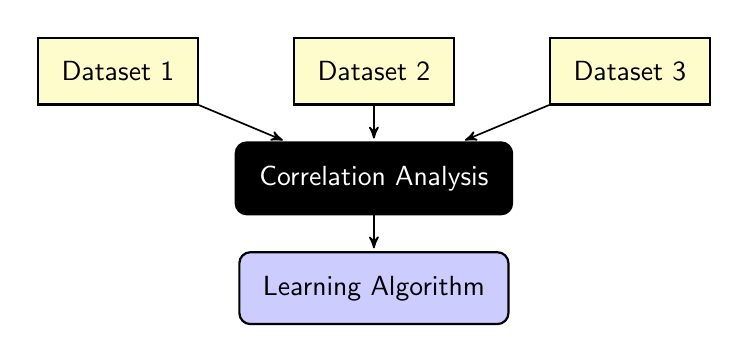
\begin{tikzpicture}[
      font=\sffamily, every matrix/.style={ampersand replacement=\&,column sep=3ex,row
      sep=3ex}, dataset/.style={draw,thick,fill=yellow!20,inner sep=.3cm},
      sink/.style={dataset,rounded corners,fill=black, text=white},
      app/.style={dataset,rounded corners,fill=blue!20}, dots/.style={gray,scale=2},
      to/.style={->,>=stealth',shorten >=1pt,semithick,font=\sffamily\footnotesize}, every
      node/.style={align=center}]

      \matrix{ \node[dataset] (dataset1) {Dataset 1}; \& \node[dataset] (dataset2)
        {Dataset 2}; \& \node[dataset] (dataset3) {Dataset 3}; \\

        \& \node[sink] (blackbox) {Correlation Analysis}; \& \\

        \& \node[app] (application) {Learning Algorithm}; \& \\ };

      \draw[to] (dataset1) -- (blackbox); \draw[to] (dataset2) -- (blackbox); \draw[to]
      (dataset3) -- (blackbox); \draw[to] (blackbox) -- (application);

    \end{tikzpicture}
    \caption{Illustration of multi-modal data fusion}
    \label{fig:data_fusion}
\end{center}
\end{figure}


\section{Canonical Correlation Analysis (CCA)}

\subsection{What is it? What is it not?}

Canonical correlation analysis (CCA) is a joint dimensionality reduction algorithm for
exactly two datasets that finds a linear transformation for each dataset such that the
correlation between the two transformed feature sets is maximized
\cite{hotelling1936relations}. CCA, however, \textit{is not} a data fusion algorithm. CCA
returns two linear transformations and a set of correlations. In this light, CCA is
extremely similar to principle component analysis (PCA), which returns a linear
transformation that accounts for the directions of largest possible variance in a
dataset. These principle components are typically used as features vectors in a variety of
machine learning algorithms. Just as PCA is a dimensionality reduction algorithm and not
the final machine learning algorithm that uses the principle components, CCA is a joint
dimensionality reduction algorithm whose dimensionality reduction ensures that datasets
are maximally correlated in their reduced spaces. These maximally correlated features may
then be used however a learning algorithm desires. 

The solution to CCA is easily found by solving a quadratic optimization problem. This
solution is a closed form expression relying on the singular value decomposition (SVD) of
a matrix product involving the covariance matrices of each dataset and the
cross-covariance between the two datasets. As these covariance matrices are rarely known
\textit{a priori}, practical uses of CCA rely on substituting sample covariance matrices
formed from training data, which we call empirical CCA.

The performance of empirical CCA has been studied previously, but insufficiently. When the
number of training samples is large compared to the dimensions of the datasets, the
performance is well understood \cite{gunderson1997estimating}. When the number of training
samples is less than the sum of the dimension of each dataset (sample deficient regime),
\cite{pezeshki2004empirical} proves that empirical CCA completely breaks down and always
reports a perfect correlation between the datasets. 

This extremely undesirable characteristic of empirical CCA has lead many to abandon CCA as
a reliable statistical analysis technique. Pezeshki, L.L. Scharf et al. argue that in this
sample deficient regime
\begin{quote}
  ... the \textcolor{red}{empirical canonical correlations are defective and
    may not be used} as     estimates of canonical correlations between random
  variables.\cite{pezeshki2004empirical}
\end{quote}
Similarly, Ge et al. conclude that
\begin{quote}
... CCA provide(s) \textcolor{red}{reliable information} about spatial
    correlations existing among pairs of data sets \textcolor{red}{only when SNRs ... are
    reasonably high, and the sample support is significantly larger than the data
    dimensions.}\cite{ge2009does}
\end{quote}



\subsection{Variations on CCA}

Due to this undesirable breakdown of CCA in the low-sample high-dimensionality regime,
many researchers proposed variations of CCA to avoid this performance loss. Most notably,
\cite{nadakuditi2011fundamental} used recent results from random matrix theory to
demonstrate that this performance breakdown may be avoided by trimming the sample
covariance matrix estimates to only include informative components. This algorithm is the
crux of this thesis. We will study its performance and develop theoretical tools in order
to use it for real-world applications. Throughout the thesis, we use the ubiquitous
low-rank signal-plus-noise model for datasets \be X = UV^H + Z, \ee where
$X=[x_1,\dots,x_n]$ is our observed data matrix whose columns are individual
multidimensional observations, $U$ is a low-rank signal subspace, $V$ is a low-rank signal
matrix, and $Z$ is a noise matrix. Surprisingly, correlation analysis for this classical
low-rank signal-plus-noise model is not completely studied. This thesis seeks to complete
the discussion. Here, we briefly touch on other variations based on CCA that do not assume
the above linear low-rank signal-plus-noise model. Many of these algorithms are tuned for
a specific application or seek to avoid the performance loss of CCA in a certain regime.

Regularized CCA (RCCA) \cite{vinod1976canonical} adds a penalty term to the magnitude of
the canonical vectors. This results in adding a scaled copy of the identity matrix to the
sample covariance matrix of each dataset, which allows each matrix to be
inverted. Therefore, RCCA returns non-trivial results in the sample-deficient
regime. However, this approach introduces a parameter to the algorithm; the effect of this
parameter is not well studied. Other variations of RCCA, such as supervised
RCCA \cite{thum2014supervised}, fast RCCA \cite{cruz2014fast}, and a multi-block RCCA
\cite{tenenhaus2014regularized}, have also been proposed.

Kernel CCA (KCCA) \cite{akaho2006kernel} was proposed to deal with non-linear correlations
existing between datasets. However, KCCA also introduces regularization parameters so as
to not return trivial solutions (see \cite{welling2005kcca} for an excellent
derivation). Besides the choice of regularization parameter, there is also ambiguity in
the choice of the kernel function, which is a common problem among kernel methods. Other
variations of KCCA have also been proposed, such as penalized KCCA
\cite{waaijenborg2009correlating}, alpha-beta divergence \cite{mandal2013non}, and CCA
based on kernel target alignment \cite{chang2013canonical}. 

Sparse CCA \cite{hardoon2011sparse} finds linear transformations such that the number of
features used is minimized. This problem is often motivated by the need for interpretable
canonical vectors that is often driven by the application, such as in brain imaging
\cite{yan2014accelerating}. There are many variations on sparse CCA, typically motivated
by application or mathematical intrigue. Sun and Keates \cite{sun2013canonical} explore
CCA in the context of censoring, Shin and Lee examine sparse functional data
\cite{shin2015canonical}, Tao et al. consider joint sparse data in
\cite{tao2014exploring}, Gao et al. explore efficient sparse CCA for high-dimensional
data \cite{gao2014efficient}, and Zhang et al. extend the analysis to multi-class group
sparse CCA \cite{zhang2013binary}. Other formulations include a penalized decomposition
\cite{witten2009penalized}, Bayesian CCA via group sparsity \cite{klami2013bayesian}, and
recursive sparse CCA \cite{chu2013sparse}.

\subsection{Applications}

CCA and its variants are widely used in a variety of fields where multiple datasets
naturally arise, the most common of which is machine learning and computer vision. In
\cite{hardoon2004canonical}, CCA is used to learn semantics of multimedia content by
fusing image and text data. Related, \cite{dhillon2011multi} uses CCA to learn word
embeddings for supervised natural language processing tasks. CCA has been widely applied
to pose estimation \cite{melzer2001nonlinear,zhai2015instance}, as this is a natural
examples where we have multiple views (image) of the same object. Other computer vision
related tasks where correlation methods are natural fits include matching people across
cameras \cite{lisanti2014matching}, clustering social event images
\cite{ahsan2014clustering}, automatic image annotation \cite{hardoon2006correlation}, and
audio-visual speaker clustering \cite{chaudhuri2009multi}.

Medical analysis is another field where there are ripe opportunities for correlation
analysis due to the vast number of modalities (EEG, MRI, CT, fMRI, MEG, etc.). CCA is
often used to determine interactions, or connectivities, between brain areas in fMRI data
\cite{deleus2011functional,arbabshirani2010comparison,khalid2013improving,guccione2013functional}
and used to fuse fMRI, sMRI, and EEG data \cite{correa2010canonical}. CCA based methods
have also been used to examine genetic connections
\cite{lin2013identifying,seoane2014canonical,lin2013group}, relying heavily on sparse
methods due to the high dimensionality of gene data and need to interpret which genes are
``on''. CCA is also a popular way to detect frequencies in steady-state visual evoked
potential (SSVEP) in brain-computer interfaces (BCIs)
\cite{zhang2013l1,nakanishi2014enhancing,zhang2014frequency}. Still further, CCA is used
in de-noising and analysis of EEG, MEG and ECG data
\cite{spuler2013spatial,campi2013non,chen2014removal,kuzilek2014comparison}.

CCA also has roots in classical signal processing applications. The authors of
\cite{via2005canonical} apply CCA to to the common communications problem of blind
equalization of single-input multiple-output (SIMO) channels. Pezeshki et al.
\cite{pezeshki2006canonical} showed that the CCA coordinates are the correct coordinates
for low-rank Gauss-Gauss detection and estimation. Scharf and Thomas
\cite{scharf1998wiener} provide a wonderful exposition on using the canonical coordinates
for Wiener filters, transform coding, filtering, and quantizing. CCA and multiset CCA have
been used to achieve joint blind source separation (BSS) in \cite{li2009joint}. CCA has
also been applied to hyperspectral imaging \cite{nielsen2002multiset}, array processing
\cite{ge2009does}, Gaussian channel capacity \cite{scharf2000canonical}, and cognitive
radio networks \cite{manco2014kernel}.

Other fun and interesting applications include climatology, finance, and music. Todros and
Hero define a new measure transformed based CCA and show its utility on financial data in
\cite{todros2012measure}. Torres et al. \cite{torres2007finding} use sparse CCA to label
portions of musical songs with meaningful words or phrases. In the field of climatology,
CCA has been used to study sea temperatures \cite{wilks2014probabilistic}, forest planning
\cite{prera2014using}, and tropical cyclones \cite{steward2014assimilating}. Finally, I
would be remiss if I didn't share my personal favorite application of CCA to date: using
CCA to analyze bovine growth \cite{li2010canonical}.

\section{Contributions of this thesis}

In many of the application presented above, researchers either have access to many
samples, or have designed an algorithm tuned specifically for a their particular
application. This thesis considers the performance of empirical correlation algorithms in
the low-sample, high dimensional setting. These algorithms are not geared toward a
particular application but are general and may be applied to any application. We will
demonstrate, both theoretically and empirically, that multi-modal correlation analysis in
this regime is a possibility. We remark that statements labeled as theorems represent, to
the best of our knowledge, new results while important results from literature are labeled
as propositions or lemmas. Chapters II-III are self contained and may be read
independently. Chapters IV-X consider the problem of correlation analysis.

Chapters \ref{sec:chpt_msd} and \ref{sec:chpt_msd_exten} consider the classical problem of
matched subspace detectors. We use insights from random matrix theory on the accuracy of
subspace estimates to derive new, optimal detectors that demonstrate the sub-optimality of
the classical plug-in detectors that simply substitute maximum likelihood estimates for
unknown parameters. Under both a stochastic and deterministic data model, we argue that
only the \textit{informative} subspace components should be used in a detector. We extend
this analysis to the case where our observations may contain missing data.

In Chapters \ref{sec:chpt_cca_det} and \ref{sec:chpt_cca_vects}, we explore the
performance of CCA and re-derive informative CCA (ICCA). We demonstrate the extreme
sub-optimality of CCA in the low-sample, high dimensionality regime. Specifically, we
provide a statistical test for both CCA and ICCA that determines whether the correlations
returned by the algorithms do indeed represent a true underlying correlation in the
datasets. We prove when each of these statistics are consistent to showcase the
superiority of ICCA. We also provide an analogous statistical test and consistency theorem
to use when the datasets have missing data entries. We create 3 new real-world,
multi-modal datasets involving video and audio to verify the performance of ICCA. We then
showcase that the canonical vectors returned by ICCA are more accurate than the CCA
vectors in the low-sample regime. Finally, we provide a new algorithm for estimating the
canonical vectors that asymptotically optimal.

Next, we explore the performance of regularized CCA (RCCA) in Chapter
\ref{sec:chpt_rcca}. When the number of training samples is limited but correlation
analysis is still desired, a common strategy is to regularize CCA by adding a penalty to
the magnitude of the linear transformation. However, we demonstrate that setting the
regularization parameter to infinity results in the best performance. In fact, in this
setting, the solution to RCCA may be found by taking the SVD of the sample
cross-covariance matrix between the two datasets. We then predict the behavior of the
largest singular values of this cross-covariance matrix assuming a low-rank
signal-plus-noise model on the individual datasets. We argue that using the top singular
values of this cross-covariance matrix to detect correlations is sub-optimal because the
correlation coefficients are coupled with the individual data signal strengths.

Using a similar proof technique, we predict the behavior of the largest singular values of
the projection of low-rank signal plus noise matrices to a smaller dimension in Chapter
\ref{sec:chpt_svd_proj}. Specifically, we consider two types of projection matrices: one
with standard complex Gaussian entries and one with orthonormal columns. We are able to
provide a closed form expression for the largest singular values in the case where the
projection matrix is unitary. Through numerical simulations, we demonstrate the
superiority of the unitary projection matrix over the Gaussian projection matrix. The
unitary projection matrix can reliably detect the signals at a lower signal-to-noise ratio
than the Gaussian projection matrix. 

In Chapter \ref{sec:chpt_det_reg} we apply CCA and ICCA to the classical problems of
detection and regression. First, we consider the low-rank signal-versus-noise subspace
detection problem given two datasets. We prove that the standard likelihood ratio test
(LRT) detector may be written using the canonical basis returned by CCA. We show that when
using empirical parameter estimates, the CCA detector is extremely suboptimal but that the
ICCA detector is equivalent to the plug-in LRT detector. We then show that the classical
Gaussian regression problem may be written in terms of the CCA basis. However, similar to
the detection problem, empirical CCA degrades the performance significantly while ICCA
matches the classical plug-in detector. We show this via mean squared error prediction
plots.

We then consider the joint problems of image retrieval and image annotation in Chapter
\ref{sec:chpt_ia}. Correlation based methods are typically overlooked as solutions to such
problems due to the problems with CCA outlined in this thesis. We show that using ICCA to
solve these problems results in non-trivial solutions. We compare the performance of CCA
and ICCA on four different image-text datasets and describe the capabilities and
limitations of ICCA in this application. When the datasets contain multiple images of the
same objects and meaningful captions, ICCA is able to capture correlations between images
and text. However, ICCA fails to capture semantic meanings between documents and
captions. We argue that with clever feature engineering and improved NLP techniques,
correlation based methods may be relevant for image retrieval and image annotation.

Lastly, we consider multi-set CCA (MCCA) in Chapter \ref{sec:chpt_mcca}. Unfortunately,
unlike CCA, there is no clear objective function to use in an optimization problem;
Kettenring \cite{kettenring1971canonical} proposes five such objective functions. Nielsen
also provides a nice formulation of MCCA in \cite{nielsen1994analysis} where he proposes
four constraint functions.  We provide derivations for these 20 formulations, in both a
theoretical and empirical setting. We then choose to consider the MAXVAR problem as we are
able to directly apply our insights from ICCA to create an informative version of it,
which we call informative MCCA (IMCCA). We demonstrate the superior performance of IMCCA
on a real-world video dataset that we created. 


\section{Problem Formulation}\label{sec:energy_detector}
We wish to design a detector that discriminates between the $H_0$ hypothesis that an
observation is purely noise and the $H_1$ hypothesis that the observation contains an
unknown signal.  We model the observation $w\in\reals^{k\times 1}$ as in
(\ref{eq:general_setup}) where $\delta=[\delta_1,\dots,\delta_k]^T\in\reals^{k\times 1}$,
with $\delta_i\neq 0$, is an unknown deterministic vector,
$z\sim\mathcal{N}\left(0,I_k\right)$ is additive white Gaussian noise (AWGN), and $k$ is
known. See
\cite{cui2013performance,santiago2013noise,arribas2013antenna,chen2013adaptive,gorji2013widely,zhou2013space,kwon2013multi,hu2013doa,liao2013direction}
for similar signal-plus-noise models in signal and array processing.  In the
Neyman-Pearson detection setting (see \cite{van1968detection}), the detector for this data
model is the likelihood ratio test (LRT)
\beq\label{eq:lrt_form}
\Lambda(w) = \frac{f\left(w\,|\, H_1\right)}{f\left(w\,|\, H_0\right)} \detgtrless \eta.
\eeq
Here $f\left(\cdot\right)$ is the appropriate conditional probability density function
(p.d.f.) of the observation and $\eta$ is a scalar threshold set so that $\Prob{\Lambda(w)
  > \eta\,|\, w\in H_0} = \alpha$ where $\alpha\in[0,1]$ is a desired false alarm rate.

The conditional distributions of $w$ modeled as in (\ref{eq:general_setup}) are
$w|H_0\sim\mathcal{N}\left(0,I_k\right)$ and
$w|H_1\sim\mathcal{N}\left(\delta,I_k\right)$. However, as $\delta$ is unknown, we cannot
substitute the p.d.f. of $w|H_1$ into (\ref{eq:lrt_form}). Instead, we use the generalized
LRT (GLRT), which maximizes $f(w|H_1)$ with respect to any unknown parameters. The GLRT
for our problem is 
\be \Lambda(w) = \frac{\max_{\delta}f\left(w\,|\,
    H_1\right)}{f\left(w\,|\, H_0\right)} \detgtrless \eta.  
\ee
The conditional p.d.f. of $w$ under the $H_1$ hypothesis is
\be
f\left(w\,|\,H_1\right) = \left(2\pi\right)^{-k/2}\exp\left\{ -\frac{1}{2}\left(w-\delta\right)^T\left(w-\delta\right)\right\}.
\ee
This p.d.f. is maximized when $\delta=w$ with the maximum value of
$(2\pi)^{-k/2}$. Substituting this into the GLRT yields
\be
\Lambda(w) = \exp\{\frac{1}{2}w^Tw\}
\ee
Taking the natural logarithm results in the test statistic
\beq\label{eq:energy_detector}
\Lambda_{\text{energy}}(w) = w^Tw = \sum_{i=1}^k w_i^2
\eeq
where $w=[w_1,\dots,w_k]^T$. This is an energy detector as its test statistic sums the
energy residing in each component (or dimension) of the given observation.

\subsection{ROC Curve Analysis}

To compare the performance of multiple detectors, we will compare their receiver operating
characteristic (ROC) curves. A ROC curve is a collection of points ($P_F,P_D$) where for
$-\infty<\eta<\infty$,
\beq\label{eq:roc}\ba
&P_F=\Prob{\Lambda(w) > \eta \,|\, w\in H_0},\\
&P_D=\Prob{\Lambda(w) > \eta \,|\, w\in H_1}.\\
\ea\eeq
For $0\leq P_F\leq 1$ we want to express the probability of detection $P_D$ as a function
of the false alarm rate, $P_F$, while noting that $P_F$ is a function of
$\eta$. To make analytical progress, we assume that $\delta$ is known for ROC
derivations. First, we compute the conditional distributions of the statistic in
(\ref{eq:energy_detector}). The conditional distributions of the components in $w$ are
simply 
$w_i|H_0\overset{\text{i.i.d.}}{\sim}\mathcal{N}\left(0,1\right)$ and
$w_i|H_1\overset{\text{i.i.d.}}{\sim}\mathcal{N}\left(\delta_i,1\right)$. Therefore,
$w_i^2|H_0\overset{\text{i.i.d.}}{\sim}\chi^2_1$ and
$w_i^2|H_1\overset{\text{i.i.d.}}{\sim}\chi^2_1\left(\delta_i^2\right)$ where $\chi^2_1$
is a chi-square random variable with one degree of freedom and $\chi^2_1(\delta_i^2)$ is a
non-central chi-square random variable with one degree of freedom and non-centrality
parameter $\delta_i^2$. As each component $w_i$ is independent,
\beq\label{eq:distr_energy} \ba
&\Lambda(w)|H_0\sim\chi^2_k,\\
&\Lambda(w)|H_1\sim\chi^2_k\left(\delta^T\delta\right), 
\ea \eeq 
where $\chi^2_k$ is a chi-square random variable with $k$ degrees of freedom and $\chi^2_k(\delta^T\delta)$ is a
non-central chi-square random variable with $k$ degrees of freedom and non-centrality
parameter $\delta^T\delta = \sum_{i=1}^k\delta_i^2$. Armed with these characterizations in
(\ref{eq:distr_energy}) and solving for $\eta$ in (\ref{eq:roc}), we can relate $P_D$ to
$P_F$ using the expression
\begin{equation}\label{eq:roc_energy}
\begin{aligned}
&P_{D_\text{energy}}(P_F,k)=1-Q_{\chi_{k}^2(\lambda_k)}\left(Q^{-1}_{\chi^2_{k}}\left(1-P_F\right)\right).\\
\end{aligned}
\end{equation}
In (\ref{eq:roc_energy}), $Q_{\chi_{k}^2}(\lambda_k)$ is the cumulative distribution function (c.d.f.) of a
non-central chi-square random variable with $k$ degrees of freedom and non-centrality
parameter $\lambda_k=\sum_{i=1}^k\delta_i^2$ and $Q_{\chi_{k}^2}$ is the c.d.f. of a chi-square random
variable with $k$ degrees of freedom. See \cite{cui2013performance,arribas2013antenna,zhou2013space} for similar ROC
performance curve derivations.

\subsection{Problem Statement}\label{sec:prob_state}

As practitioners, we can control which signal components that the energy detector in
(\ref{eq:energy_detector}) uses. Without loss of generality, we assume that the entries of
$\delta$ are ordered (i.e. $|\delta_1| \geq |\delta_2| \geq\dots|\delta_k|$). With this
assumption, we can decide how many signal components, $d$, to use in the energy detector
\beq\label{eq:the_detector} 
\Lambda_d(w) = \sum_{i=1}^d w_i^2.
\eeq 
Specifically, we wish to answer the following question:
\begin{quote}
  Given a signal vector $\delta$ and a desired false alarm rate $P_F$, how many signal
  components, $d$, maximize $P_{D_{\text{energy}}}(P_F,d)$ in (\ref{eq:roc_energy}) for an
  energy detector with the form of (\ref{eq:the_detector}) derived from observations
  as in (\ref{eq:general_setup})? 
\end{quote}
Answering this question will provide some surprising results. We will show that if the
components $\delta_i$ are too small in magnitude, including them in a detector actually
degrades performance. The setting where $\delta_i$ equals zero is a special case where not
including it will always yield a performance gain.

\section{Useful Components In Energy Detectors}\label{sec:useful}
In this section, we answer the question posed at the end of Section
\ref{sec:energy_detector} by defining $\kuse$, the number of useful signal components. We
show that $\kuse$ is dependent on $\delta$ and the desired false alarm rate $P_F$. We
provide some intuition behind our definition by discussing how the conditional
distributions of the energy detector's test statistic shift when adding additional
components. If an additional signal component further separates the conditional
distributions, it is one of the $\kuse$ components in detection; otherwise, including that
component would degrade detector performance. Of particular importance, $\kuse$ may be
less than the inherent dimension, $k$, of the observed data, even when $\delta_i\neq0$.

\subsection{Definition and Computation of $\kuse$}

We define the number of useful detection components at a false alarm rate $P_F$ as the
solution to the following optimization problem
\beq\label{eq:opt_prob}
\kuse = \argmax_{d\in\{1,\dots,k\}} P_{D_{\text{energy}}}(P_F,d)
\eeq 
where $P_{D_{\text{energy}}}(P_F,d)$ is defined in (\ref{eq:roc_energy}). This is the
optimal number of components to include in an energy detector in (\ref{eq:the_detector})
to maximize detector performance. Using exactly $\kuse$ components includes all components
that improve detection ability and excludes all components that degrade detection ability.

To determine $\kuse$, we propose the greedy ``algorithm'' in Figure \ref{algo:kuse}. The
algorithm relies on the fact that the components of $\delta$ are ordered
(i.e. $|\delta_1|\geq\dots|\delta_k|$). It adds one component at a time and searches for
the last component that resulted in an increase in detection ability. This algorithm
relies on knowledge of $\delta$ and so by definition $\kuse$ is an oracle quantity.
Therefore, a realizable detector using exactly $\kuse$ components is currently beyond
reach. Estimating $\kuse$ is a topic for future work and may involve placing a prior
distribution on the test vector. In Section \ref{sec:msd}, we discuss using the effective
number of subspace components, $\keff$, as an estimate for $\kuse$.

%\begin{figure}
% \hrulefill
%  \begin{algorithmic}[1]


\begin{algorithm}
  \KwIn{$P_F$, $\delta$ }

  Compute $P_D(P_F,1)$ from (\ref{eq:roc_energy})

  \For{$h=2,\dots,k$} {

    Compute $P_D(P_F,h)$ from (\ref{eq:roc_energy})

    \If{$P_D(P_F,h) < P_D(P_F,h-1)$}{

      $\kuse= h-1$

      \textbf{Return:} $\kuse$
    }
  }
  $\kuse = k$

  \KwOut{$\kuse$ }
  \caption{Algorithm to determine $\kuse$. This is computable in an oracle setting\\
    where $\delta$ is known.}  
  \label{algo:kuse}
\end{algorithm}

\subsection{Discussion of Test Statistic Distributions}

In order to provide intuition behind the definition of $\kuse$, we examine the conditional
distribution of the test statistic in (\ref{eq:the_detector}):
\beq\label{eq:d_distrs}\ba
& \Lambda_d(w)\,|\,H_0 \sim\chi^2_d,\\
& \Lambda_d(w)\,|\,H_1 \sim\chi^2_d(\lambda_d)\\
\ea\eeq
where
\beq\label{eq:nc_param}
\lambda_d = \sum_{i=1}^d \delta_i^2.
\eeq
Clearly, both distributions and the non-centrality parameter depend on $d$. Therefore, a
closed form expression for $\kuse$ is not possible and we rely on the greedy algorithm
in Figure \ref{algo:kuse}. Adding an additional component presents a tradeoff between
adding $\delta_i^2$ to the non-centrality parameter and adding 1 to the degrees of
freedom in the c.d.f's in (\ref{eq:d_distrs}).

This tradeoff becomes more evident when using (\ref{eq:roc_energy}) to rewrite the
optimization problem in (\ref{eq:opt_prob}) as
\beq\label{eq:simple_opt}
\kuse = \argmin_{d\in\{1,\dots,k\}}
Q_{\chi_{d}^2(\lambda_d)}\left(Q^{-1}_{\chi^2_{d}}\left(1-P_F\right)\right). 
\eeq

By fixing the signal distribution $Q_{\chi^2_d(\lambda_d)}$, solving (\ref{eq:simple_opt}) is
equivalent to minimizing $Q^{-1}_{\chi^2_{d}}\left(1-P_F\right)$, which is achieved when
$d=1$. This minimizes the variance contribution from the noise distribution. However, by
fixing the noise distribution $Q_{\chi^2_d}$, solving (\ref{eq:simple_opt}) is equivalent
to minimizing $Q_{\chi_{d}^2(\lambda_d)}\left(\cdot\right)$, which is achieved when
$d=k$. This maximizes the variance contribution from the signal distribution. The solution
to (\ref{eq:simple_opt}) is dependent on how much each additional component contributes to
the overall non-centrality parameter. If the contribution is large enough, the added
variance in the noise distribution from the extra degree of freedom is overcome by the
distribution shift induced by the increase in non-centrality parameter.

To illustrate how the conditional distributions shift when adding components to the energy
detector, Figure \ref{fig:distributions} plots the distributions of $\Lambda_d(w)|H_0$ and
$\Lambda_d(w)|H_1$ for three choices of $d$ and $\lambda_d$. Figure \ref{fig:small} sets
$d=1$ and $\lambda_d=2$ and is used as a baseline. Figure \ref{fig:med} increases the
number of components to $d=2$ while keeping the non-centrality parameter fixed at
$\lambda_d=2$. The added component increases the noise variance by 2. However, as there is
no increase in the non-centrality parameter, the signal variance also increases by
2. Thus, the signal-to-noise ratio is effectively decreased. Therefore, the second
component causes the conditional distributions to become more similar and thus degrades
detector performance; therefore, $\kuse=1$. Figure \ref{fig:big} keeps the number of
components at $d=2$ but increases the non-centrality parameter to $\lambda_d=3$. In this
setting, the increase in non-centrality parameter increases the signal variance, which
overcomes the resulting increase in noise variance. The second component further separates
the conditional distributions and improves detection performance; therefore,
$\kuse=2$. Figure \ref{fig:dist_roc} plots the corresponding ROC curves for the three
choices of parameters in Figure \ref{fig:distributions}. When adding a component causes
the conditional distributions to better separate as in Figure \ref{fig:big}, the resulting
ROC curve shows an improvement in detection. \textit{For an additional component to be one
  of the $\kuse$ components, the resulting increase in noise variance must be overcome by
  a sufficiently large enough increase in non-centrality parameter.}

\begin{figure}[t]
\centering
\subfigure[$d=1$, $\lambda_d=2$]{
  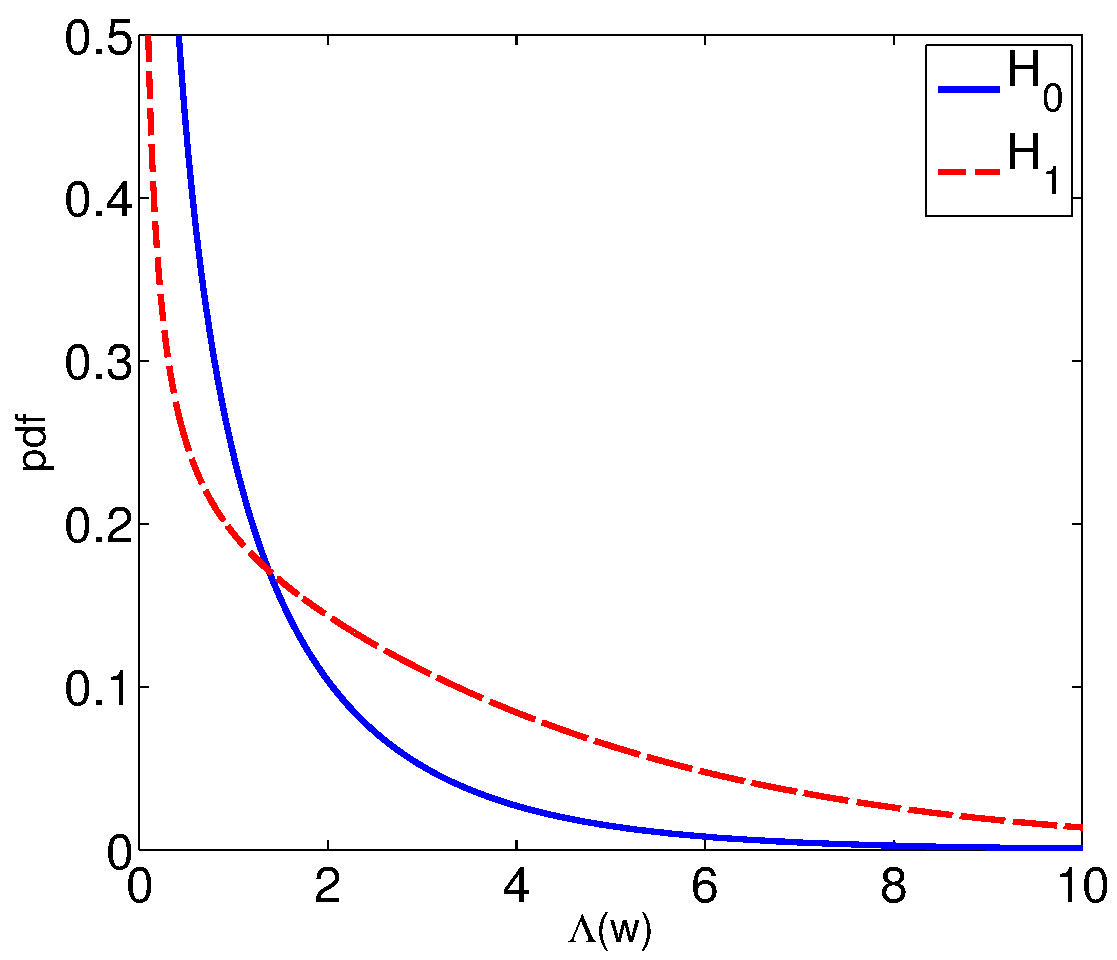
\includegraphics[width=0.3\textwidth]{taes_msd/figures/dist1.pdf}
  \label{fig:small}}
\subfigure[$d=2$, $\lambda_d=2$]{
  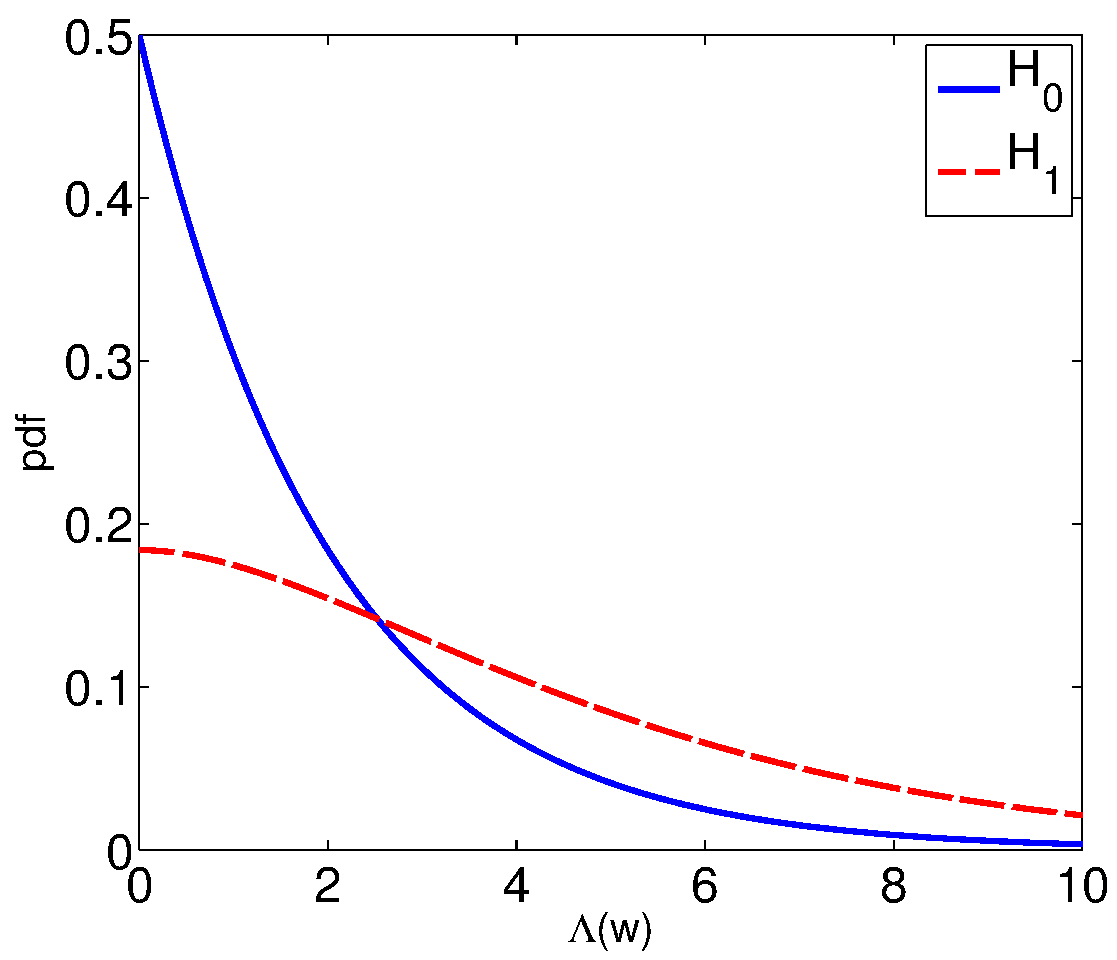
\includegraphics[width=0.3\textwidth]{taes_msd/figures/dist2.pdf}
  \label{fig:med}}
\subfigure[$d=2$, $\lambda_d=3$]{
  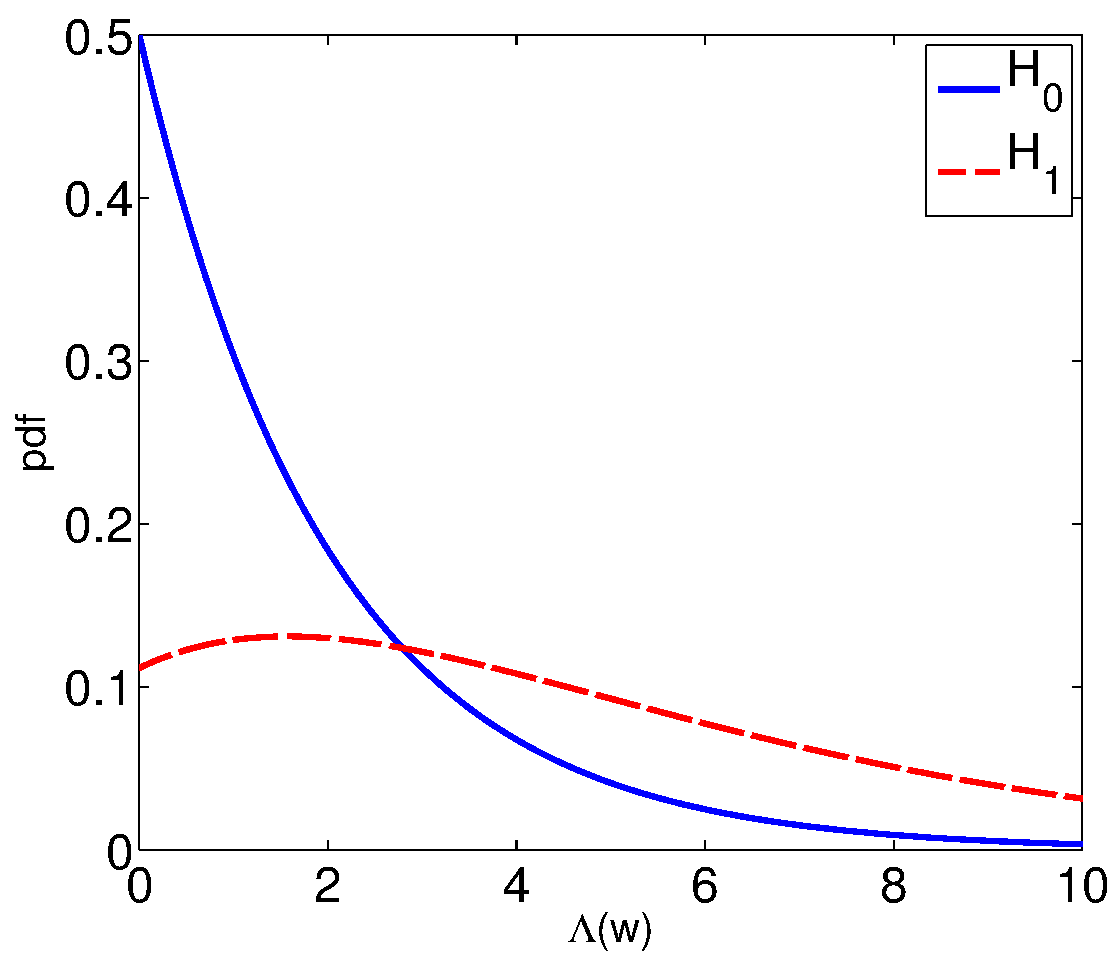
\includegraphics[width=0.3\textwidth]{taes_msd/figures/dist3.pdf}
  \label{fig:big}}
\caption{Probability density function (p.d.f.) of $\Lambda(w)\,|\,H_0$ and
  $\Lambda(w)\,|\,H_1$ for three combinations of the number of components $d$ and
  non-centrality parameter $\lambda_d$. (a) Baseline: $d=1$, $\lambda_d=2$ (b) Increases $d$
  but keeps $\lambda_d$ fixed. The distributions are less separable. (c) Increases both $d$
  and $\lambda_d$. The distributions are more separable.}
\label{fig:distributions}
\end{figure}

\begin{figure}[t]
  \centering
  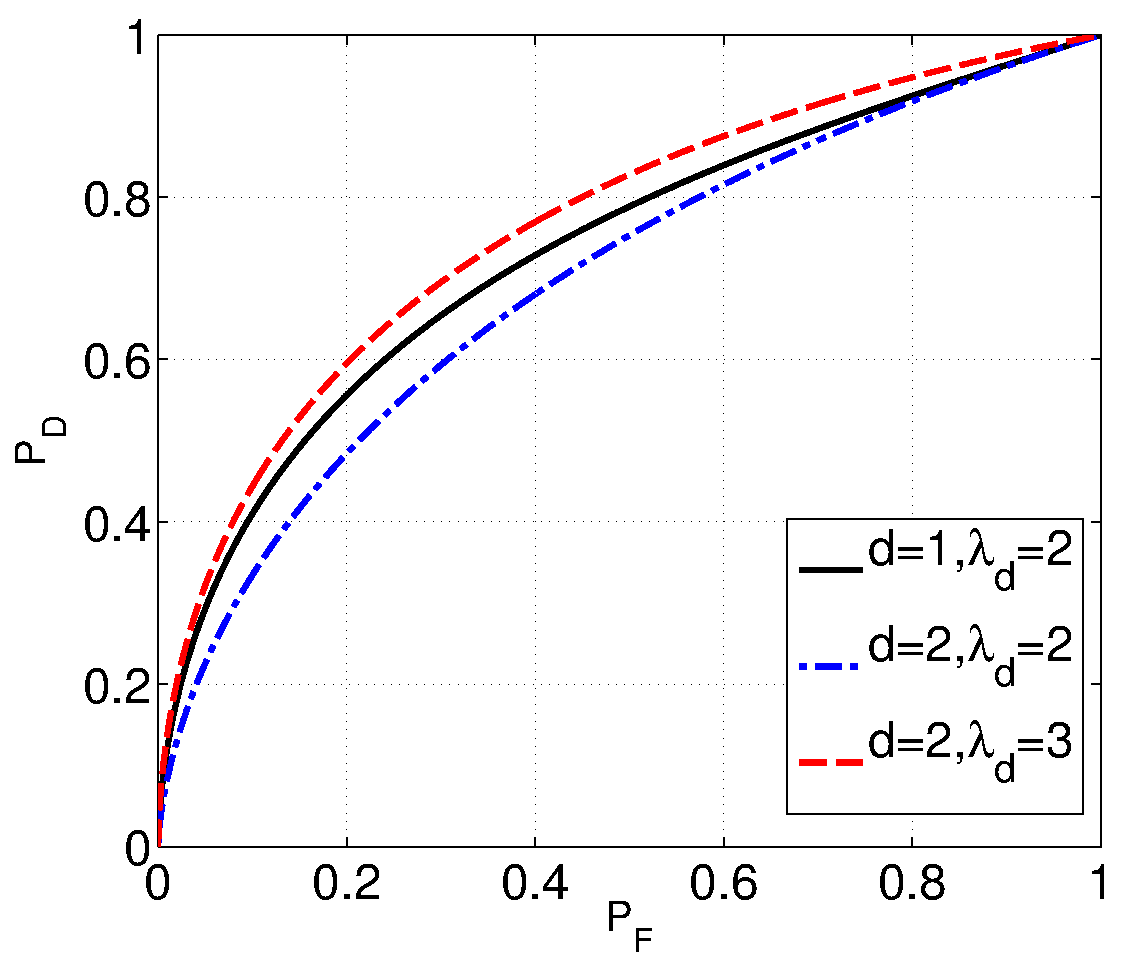
\includegraphics[width=\figwidth]{taes_msd/figures/dist_roc.pdf}
  \caption{The corresponding ROC curves to the three choices of $d$ and $\lambda_d$ in
    Figure \ref{fig:distributions}. ROC curves were generated from (\ref{eq:roc}). When
    adding an additional subspace component, the non-centrality parameter must increase
    sufficiently in order to achieve improved detection. }
  \label{fig:dist_roc}
\end{figure}

Finally, we explore the minimum increase in non-centrality parameter needed to improve
detection ability. Consider a setting with $d=1$ component and corresponding
non-centrality parameter $\lambda_1$. Let $\lambda_2$ be the resulting non-centrality
parameter by adding a second component, $d=2$, and let $\Delta\lambda=\lambda_2-\lambda_1$
be the resulting increase in non-centrality parameter. Figure \ref{fig:nc_lines} plots the
minimum increase in non-centrality parameter needed to improve detection as a function of
$\lambda_1$ for a few choices of $P_F$. If the increase in non-centrality parameter
exceeds this minimum threshold, that component is one of the $\kuse$ components.

We observe that the minimum increase in non-centrality parameter is dependent both on the
desired false alarm rate, $P_F$, and the first non-centrality parameter, $\lambda_1$.

The minimum increase in non-centrality parameter is larger for smaller false alarm rates
and is larger for larger $\lambda_1$. This is intuitive because larger values of
$\lambda_1$ separate the conditional distributions very well, indicating that the first
component is an excellent discriminant between the two hypotheses $H_0$ and $H_1$. For the
second component to improve detection ability, its contribution to the non-centrality
parameter must be larger for larger $\lambda_1$. Otherwise, the second component only adds
more noise to the detector. More generally, for the $i$th component to be one of the
$\kuse$ components, $\delta_i^2$ must exceed a critical threshold that is dependent on
$\sum_{j=1}^{i-1}\delta_j^2$. 

\begin{figure}[t]
\centering
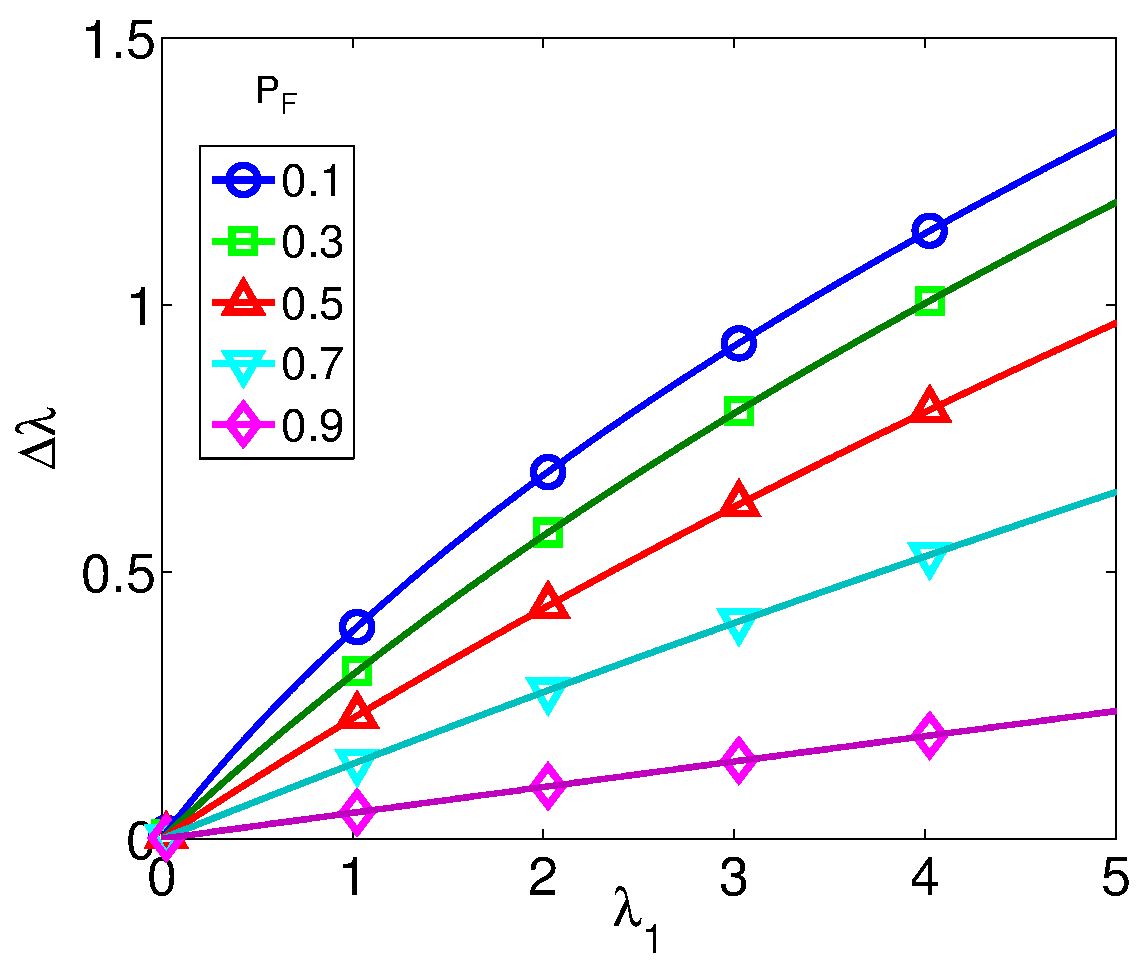
\includegraphics[width=\figwidth]{taes_msd/figures/nc_lines.pdf}
\caption{Minimum increase in non-centrality parameter necessary for increased detector
  performance. Results are shown for multiple choices of $P_F$. $\lambda_1$ indicates the
  non-centrality parameter when $d=1$ and $\Delta\lambda$ indicates the increase in
  non-centrality parameter when increasing the number of components to $d=2$.}
\label{fig:nc_lines}
\end{figure}


\section{Useful Components in Deterministic Matched Subspace Detectors}\label{sec:msd}
This section will apply the results in Section \ref{sec:useful} about useful components to
deterministic matched subspace detection. In this detection setting, we are given a high
dimensional test observation and wish to discriminate between the $H_0$ hypothesis that
the observation is purely noise and the $H_1$ hypothesis that the observation contains a
low-rank-$k$ signal that lies at a fixed point in an unknown subspace. To design a
detector, we have access to a training dataset of signal bearing observations.
We assume that the training data was collected in a variety of representative experimental
conditions, allowing each observation's signal component to lie at a different location in
the signal subspace. This setup is the similar to that in \cite{asendorf2013performance}
and the resulting standard matched subspace detector is an energy detector with the same
form as (\ref{eq:the_detector}). We use random matrix theory to determine the number of
informative subspace components, $\keff$, which is an upper bound for
$\kuse$. Through a numerical example, we demonstrate the relationship between the standard
plug-in detector using exactly $k$ subspace components, a detector using $\keff$ subspace
components, and a detector using exactly $\kuse$ subspace components.

\subsection{Training Data Model}\label{sec:training_data}

Let $U=[u_1,\dots,u_k]\in\reals^{n\times k}$ be an unknown signal subspace matrix with
pairwise orthonormal columns $u_i\in\reals^{n\times 1}$. To estimate $U$, 
we are provided a dataset containing $m$ signal-bearing training vectors
$y_i\in\reals^{n\times 1}$, $i=1,\dots,m$, modeled as 
\beq\label{eq:taes_train}
y_i=Ux_i+z_i 
\eeq 
where
$z_i\overset{\text{i.i.d.}}{\sim}\mathcal{N}(0,I_n)$ and
$x_i\overset{\text{i.i.d.}}{\sim}\mathcal{N}(0,\Sigma)$ where
$\Sigma=\diag(\sigma_1^2,\dots,\sigma_k^2)\in\reals^{k\times k}$ with
$\sigma_1>\sigma_2>\dots>\sigma_k>0$ known. For each observation, $x_i$ and $z_i$ are
independent. In the training data, $x_i$ is modeled stochastically to represent the
variety of conditions under which the training data may be collected.  We assume that the
dimension, $k$, of our subspace is known and that $k\ll n$ so that we have a low-rank
signal embedded in a high-dimensional observation vector. Applications in which training
datasets arise include MIMO radar \cite{chen2013adaptive}, GNSS receivers
\cite{arribas2013antenna}, source localization \cite{he2013near}, DOA
\cite{liao2013direction}, and target detection \cite{kwon2013multi}. In such applications,
we may think of the entries of $y_i$ received data from an antenna array, $U$ as the
channel response matrix, $x_i$ as the transmitted waveform, $\Sigma$ as the signal-to-noise
ratio (SNR) matrix, and $z_i$ as additive noise.

\subsection{Testing Data Model}

In the testing setting, we are given an unlabeled observation $y\in\reals^{n\times 1}$
modeled as
\begin{equation}\label{eq:determ_setup}
y=\left\{
\begin{aligned}
&z
&& y\in H_0:\text{ Noise only}\\
&U\Sigma^{1/2} x+z
&& y\in H_1:\text{ Signal-plus noise}\\
\end{aligned}\right. ,
\end{equation}
where $U$, $\Sigma$, and $z$ are modeled the same as the training data as described in
Section \ref{sec:training_data}. However, for the test observations, $x=[x_1,\dots,x_k]^T$
is a non-random, unknown deterministic vector. Thus the signal, $U\Sigma^{1/2}x$, lies at a
fixed point in the unknown subspace. Note that $\Sigma$ controls the SNR of each subspace
component.

\subsection{Subspace Estimation and Accuracy}\label{sec:param_estim}

In the testing model, the signal subspace $U$ is unknown and must be estimated from the
provided training data. Given the signal bearing training data 
\be
Y = \left[ y_1, \dots, y_m \right]\in\reals^{n\times m},
\ee 
we form the sample covariance matrix
$S=\frac{1}{m}YY^{T}$. The covariance matrix of a training observation is $\E{y_iy_i^T} = U\Sigma
U^T +I_n$ and it follows that the (classical) maximum likelihood estimates (in the many-sample, small
matrix setting) for $U$ is given by 
\beq\label{eq:param_estims_stoch}
\widehat{U}=[\widehat{u}_1 \dots \widehat{u}_{k}] \eeq
where
$\widehat{u}_1,\dots,\widehat{u}_{k}$ are the eigenvectors of $S$ corresponding to the
largest $k$ eigenvalues \cite{muirhead1982aspects} .

In any real world setting, we have finite training data and finite SNR. Therefore,
$\widehat{U}$ is inaccurate and degrades the performance of any detector that relies on it.
Proposition 5.1 of \cite{asendorf2013performance}  characterized the asymptotic accuracy of the
eigenvectors of the sample covariance matrix $S$ stating that as $n,m\to\infty$ with $c=n/m$
\beq\label{eq:angles}
|\langle u_i,\widehat{u}_i\rangle|^2 \convas
\begin{cases}
\dfrac{\sigma_i^4-c}{\sigma_{i}^4+\sigma_{i}^2c} & \text{ if } \sigma_{i}^2>\sqrt{c}\\
0 & \textrm{otherwise}\\
\end{cases}.  \eeq We note that $\convas$ denotes almost sure convergence. The key insight
to (\ref{eq:angles}) is that only the eigenvectors corresponding to the signal variances,
$\sigma_i^2$, lying above the phase transition $\sqrt{c}$ are
\textit{informative}. Following \cite{asendorf2013performance, nadakuditi2008sample}, we
define the effective number of (asymptotically) identifiable subspace components
$k_\text{eff}$ as:
\begin{equation}\label{eq:keff}
k_\text{eff} = \text{Number of } \sigma_i^2 > \sqrt{c}.
\end{equation}

\subsection{Plug-in and RMT Detectors}

If $U$ was known, the matched subspace detector is the GLRT using the test statistic (see
\cite{scharf1994matched,vincent2008matched,fuchs2007robust})
\be
\Lambda(w) = y^TUU^Ty = w^Tw
\ee
where $w=U^Ty\in\reals^{k\times 1}$. This is clearly an energy detector of the same form as
(\ref{eq:the_detector}) where each component of $w$ is the energy of $y$ residing in that
direction of the subspace. However, this detector is not realizable as $U$ is unknown and
so we substitute $\widehat{U}$ for the unknown $U$, resulting in the plug-in detector
\cite{asendorf2013performance}
\beq\label{eq:plugin_stat}
\Lambda_{\text{plugin}}(\widehat{w})= \widehat{w}^T\widehat{w} = \sum_{i=1}^k \widehat{w}_i^2
\eeq 
where $\widehat{w} = \widehat{U}^T y$ is the projection of the test observation onto the
estimated subspace. Similar plug-in techniques using sample covariance matrices occur in
direction detection \cite{santiago2013noise} and GNSS receivers \cite{arribas2013antenna}. The plug-in detector incorrectly assumes that $\widehat{U}=U$ and consequently
that all $k$ subspace components are informative. To avoid some of the performance loss of the
plug-in detector associated with including uninformative subspace components, we derived a
RMT detector that only includes the informative subspace components (see \cite{asendorf2013performance} for a derivation). The
RMT detector statistic is 
\beq\label{eq:rmt_stat}
\Lambda_{\text{rmt}}(\widehat{w})= \sum_{i=1}^{\keff}\widehat{w}_i^2.
\eeq

Clearly, both the plug-in and RMT detectors are energy detectors of the form in 
(\ref{eq:the_detector}) and so we may use (\ref{eq:roc_energy}) to analyze the performance
of each detector. In the MSD application, $\delta_i = \sigma_i|\langle
u_i,\widehat{u}_i\rangle| s_i x_i$ where $s_i\in\left\{1,-1\right\}$ represents the
random phase ambiguity in the eigenvector computation. Therefore, the non-centrality
parameter for this problem is 
\beq\label{eq:msd_nc_param}
\lambda_d = \sum_{i=1}^d \sigma_i^2|\langle u_i,\widehat{u}_i\rangle|^2x_i^2
\eeq
where the plug-in detector uses $d=k$ subspace components and the RMT detector uses
$d=\keff$ subspace components. In \cite{asendorf2013performance}, we demonstrated that the
plug-in detector is suboptimal and that the RMT detector will always achieve the same or
better performance.

\subsection{Relationship between $\kuse$ and $\keff$}

We first note that $\kuse\leq\keff$. If a subspace component is uninformative ($|\langle
u_i,\widehat{u}_i\rangle|^2 =0$ as determined by (\ref{eq:keff})), that component
contributes nothing to the non-centrality parameter as defined in
(\ref{eq:msd_nc_param}). From the analysis in Section \ref{sec:useful}, including this
subspace component in a detector would degrade detector performance. Therefore, a subspace
component must be informative to be one of the $\kuse$ subspace components. 

However, the number of useful subspace components may be strictly less than the number of
informative subspace components. As demonstrated in Figure \ref{fig:nc_lines}, when adding
an additional subspace component, the increase in non-centrality parameter must exceed a
minimum value. Examining (\ref{eq:msd_nc_param}), the non-centrality parameter depends on
$\Sigma$, $x$, and the accuracy of the eigenvectors of the sample covariance matrix
($|\langle u_i, \widehat{u}_i\rangle|^2$). Depending on these values, adding the $i$-th
component may not increase the non-centrality parameter enough to improve detection, even
when the subspace component is informative ($|\langle u_i,
\widehat{u}_i\rangle|^2>0$). Thus, it is possible for informative subspace components to
not be useful in detection.

Besides the desired false alarm rate, $P_F$, $\kuse$ also depends on $\Sigma$ and $x$ for
the matched subspace detector. Larger values of $|x_i|$ and $\sigma_i$ lead to larger
non-centrality parameters as defined in (\ref{eq:msd_nc_param}), making it more likely for
that component to be useful.  This is intuitive because the larger $|x_i|$ and $\sigma_i$
force the mean of the conditional distribution of $\widehat{w}_i|H_1$ further from 0,
which is the mean of the conditional distribution of $\widehat{w}_i|H_0$.  If we
instead fix $\Sigma$, $n$ , and $x$ and allow $m$ to change, we observe that more training
data increases the accuracy the subspace estimate as seen in (\ref{eq:keff}). Therefore,
increasing $m$ increases $\delta_i$, which may make subspace components useful.

The number of informative subspace components, $\keff$, is an upper bound for the number
of useful subspace components, $\kuse$. As mentioned earlier, we cannot compute $\kuse$ in
closed form because the deterministic vector $x$, which drives the non-centrality
parameters $\delta_i$, is unknown. Therefore, $\kuse$ is an oracle statistic as so we use
$\keff$ as a proxy for $\kuse$ in a realizable detector. However, as $\keff$ does not depend
on $x$, whenever $\keff\neq\kuse$, detectors using $\keff$ subspace components will be
suboptimal.

Finally, we note that the derivation and computation of $\kuse$ for the matched subspace
detection application relies on random matrix theory. Without these insights, we would
have no expression for $|\langle u_i,\widehat{u}_i\rangle|^2$ and subsequently could not
compute the non-centrality parameter in (\ref{eq:msd_nc_param}) to use in the algorithm in
Figure \ref{algo:kuse}.

\subsection{Numerical Example}

In Figure \ref{fig:main_result} we compare the performance of the plug-in and RMT
detectors to the performance of a detector that uses $d=\kuse$ subspace components. We
consider the setting when $k=3$, $n=200$, $\Sigma=\diag(5,2,0.5)$, and
$x=[1.5,1.5,1.5]^T$. For a fixed $P_F=0.1$, Figure \ref{fig:det_perf} plots the
theoretical detection probability (as computed in (\ref{eq:roc_energy}) using
(\ref{eq:keff}) and (\ref{eq:msd_nc_param})) given various amounts of training
data. Results are shown for the plug-in ($d=k$), RMT ($d=\keff$), and useful ($d=\kuse$)
detectors. Figure \ref{fig:dvals} plots the
corresponding number of subspace components each uses given various amounts of training
data.

\begin{figure}[t]
\centering
\subfigure[Detector Performance]{
  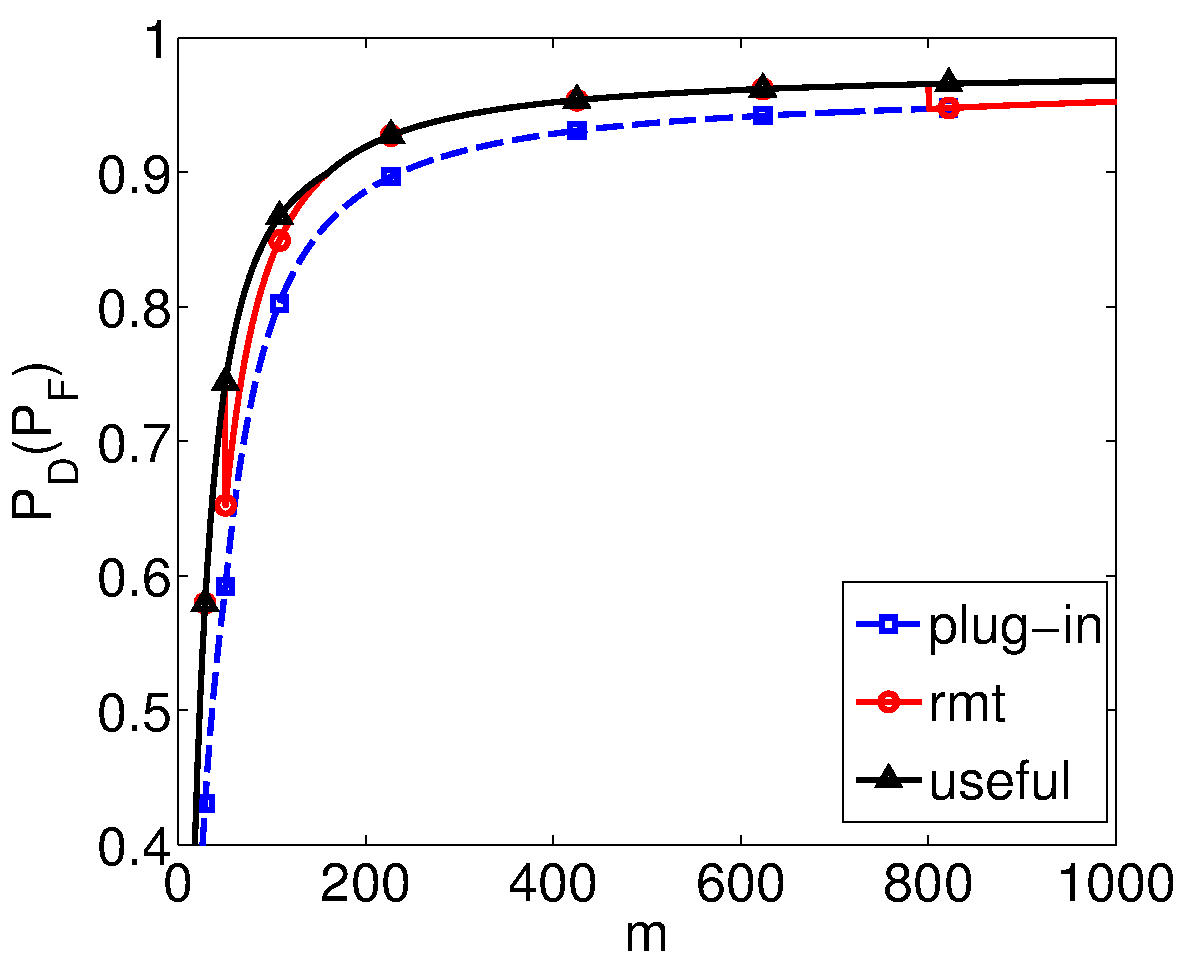
\includegraphics[width=0.45\textwidth]{taes_msd/figures/taes_pd_v_m.pdf}
  \label{fig:det_perf}}
\subfigure[Number of Subspace Components]{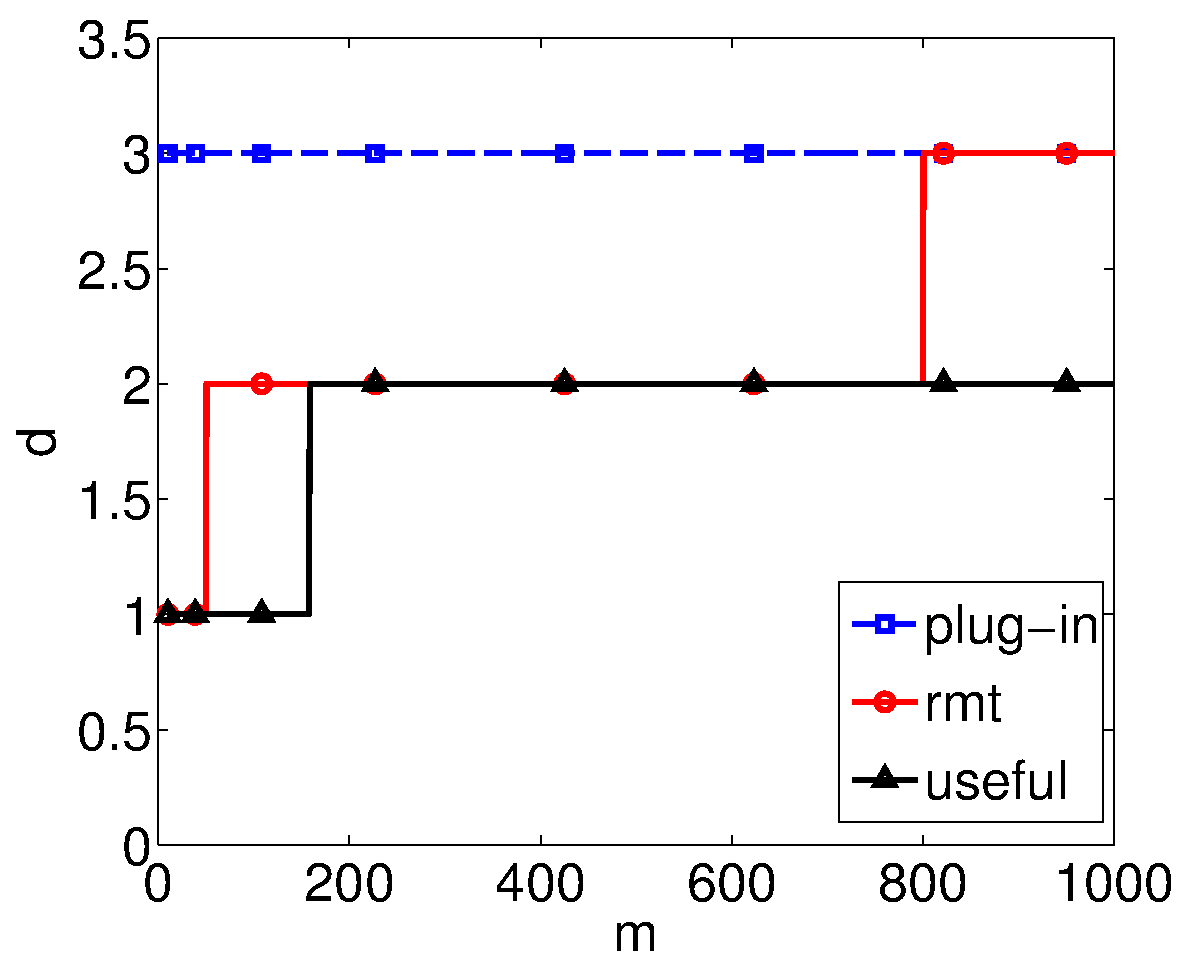
\includegraphics[width=0.45\textwidth]{taes_msd/figures/taes_d_v_m.pdf}
  \label{fig:dvals}}
\caption{Deterministic energy detector performance as a function of the number of training
  samples. In this experiment $n=200$, $\Sigma =\diag(5,2,0.5)$, $x=[1.5,1.5,1.5]^T$, and
  the required false alarm rate is $P_F=0.1$. (a) The theoretical probability of detection
  achieved by the plug-in, RMT, and useful detectors. $P_D(P_F)$ is calculated in
  (\ref{eq:roc}). The plug-in detector sets $d=k$, the RMT detector sets $k=\keff$ as
  defined in (\ref{eq:keff}), and the useful detector sets $d=\kuse$ as calculated in
  Figure \ref{algo:kuse} using the non-centrality parameter defined in
  (\ref{eq:msd_nc_param}). The useful detector achieves the optimal performance. (b) The
  number of subspace components used by the plug-in, RMT, and useful detectors. Whenever
  $\keff\neq\kuse$, the RMT detector realizes a suboptimal detector performance. Even
  though these subspace components are \textit{informative}, there is not enough training
  data to make them \textit{useful} in detection.}
\label{fig:main_result}
\end{figure}

Evident in Figure \ref{fig:det_perf}, the detector using $\kuse$ subspace components
achieves the maximum detection ability of all detectors for every amount of training
samples. This is slightly contrived because $\kuse$ is optimized to do just this. More
importantly, we empirically see that using $\keff$ subspace components is not always
optimal.  However, examination of Figure \ref{fig:dvals} reveals why this occurs. For
$50\leq m\leq 160$, $\keff=2>\kuse=1$. Therefore, even though the second subspace
component is informative by definition, it is not \textit{useful} in detection. Including
it in an energy detector decreases detector performance. A similar phenomenon
occurs at $m=800$ when $\keff$ increases to 3 but $\kuse$ remains constant at 2. Unlike
the RMT detector, the detection performance of the useful detector increases monotonically
with an increase in training samples. Both the RMT and useful detectors outperform the
standard plug-in detector which uses all $k$ subspace components.


\section{Extension - Weighted Energy Detector}\label{sec:ext}
The energy detector in (\ref{eq:energy_detector}) may be generalized by adding a
non-negative weight to each component in the sum. The statistic for the
weighted energy detector is 
\beq\label{eq:weighted_detector}
\Lambda_{\text{weighted}}(w) = w^TAw = \sum_{i=1}^k a_iw_i^2.
\eeq
where $A=\diag(a_1,\dots,a_k)\in\reals^{k\times k}$ and $a_i\geq0$. We constrain $\sum_{i=1}^k a_i = 1$ so that the weights
reside on the $(k-1)$-simplex. This reduces the set of possible weights by eliminating
those that are multiples of each other, which results in equivalent
detectors. The weighted energy detector gives practitioners additional design freedom to
maximize detector performance. Using a similar analysis as in Section
\ref{sec:energy_detector}, the conditional distributions of the weighted energy detector's 
statistic in (\ref{eq:weighted_detector}) are
\beq\label{eq:roc_weighted}
\ba
&\Lambda(w)|H_0\sim\sum_{i=1}^k a_i\chi_{1i}^2,\\
&\Lambda(w)|H_1\sim\sum_{i=1}^k a_i \chi_{1i}^2\left(\delta_i^2\right),
\ea
\eeq
where $\chi_{1i}^2$ are independent chi-square random variables with one degree of freedom
and $\chi_{1i}^2\left(\delta_i^2\right)$ are independent non-central chi-square random variable
with one degree of freedom and non-centrality parameter $\delta_i^2$. We can relate $P_D$
to $P_F$ using the expression
\beq\label{eq:weighted_pd}
P_{D_{\text{weighted}}}(P_F,A) = 1 - Q_{\Lambda|H_1}\left(Q^{-1}_{\Lambda|H_0}(1-P_F)\right)
\eeq
where $Q_{\Lambda|H_1}$ is the c.d.f of $\Lambda(w)|H_1$ in (\ref{eq:roc_weighted})
and $Q_{\Lambda|H_0}$ is the c.d.f. of $\Lambda(w)|H_0$ in (\ref{eq:roc_weighted}). 

The definition of $\Lambda_{\text{weighted}}(w)$ in (\ref{eq:weighted_detector}) raises
the natural question 
\begin{quote}
  Given $\delta$ and a desired $P_F$, what is the optimal choice of weighting matrix, $A$,
  that maximizes $P_{D_{\text{weighted}}}(P_F)$ for a weighted energy detector with the
  form of (\ref{eq:weighted_detector}) using observations generated from
  (\ref{eq:general_setup})?
\end{quote}
While the c.d.f. of chi-square and non-central chi-square random variables are known in
closed form, the c.d.f. of a weighted sum of chi-square random variables is not known in closed
form and therefore (\ref{eq:weighted_pd}) cannot be computed analytically. It is common
to use saddlepoint approximation techniques \cite{wood1993saddlepoint} to compute the
c.d.f. of such sums in (\ref{eq:roc_weighted}), however, such techniques must be computed
for many thresholds, $\eta$, to generate a ROC curve for one weighting matrix $A$. To
optimize over $A$ in (\ref{eq:weighted_pd}), this process would need to be repeated over a
discretization of the ($k-1$)-simplex. Developing a more efficient algorithm to optimize
over the weighting matrix, $A$, is an important topic for future work.

To illustrate how weighted energy detectors can improve detection performance, consider a rank-2 setting where the desired
false alarm rate is $P_F=0.1$. Optimizing $A=\diag(a_1,a_2)$ on the simplex $a_1+a_2=1$
results in one degree of freedom and so
\be
\Lambda(w)_{\text{weighted}} = aw_1^2 + (1-a)w_2^2  
\ee
where $a\in[0,1]$. Figure \ref{fig:weighted} plots the empirically achieved (see
\cite{fawcett2006introduction}) probability of detection as a 
function of the weighting parameter $a$ for four detectors each with a different signal
vector $\delta$. Figure \ref{fig:weights_easy} shows results for detectors using
$\delta=[1,1]^T$ and $\delta=[1,0]^T$. The detector with $\delta=[1, 1]^T$ achieves
maximum performance when $a=0.5$, which weights both components equally. As
$\delta_1=\delta_2=1$ both $w_1$ and $w_2$ have the same conditional distributions and it
is intuitive that we weight both components equally. However, the detector using
$\delta=[1, 0]^T$ achieves maximum performance when $a=1$ indicating that the second
component is not useful in detection. As $\delta_2=0$, $w_2$ has the same distribution
under both the $H_1$ and $H_0$ hypotheses, giving it no discriminatory power. For these
values of $\delta$, the optimal $a$ is obvious and the performance of the weighted energy
detector is the same as that of the standard energy detector.

\begin{figure}[t]
\centering
\subfigure[Easy Optimal Weights]{
  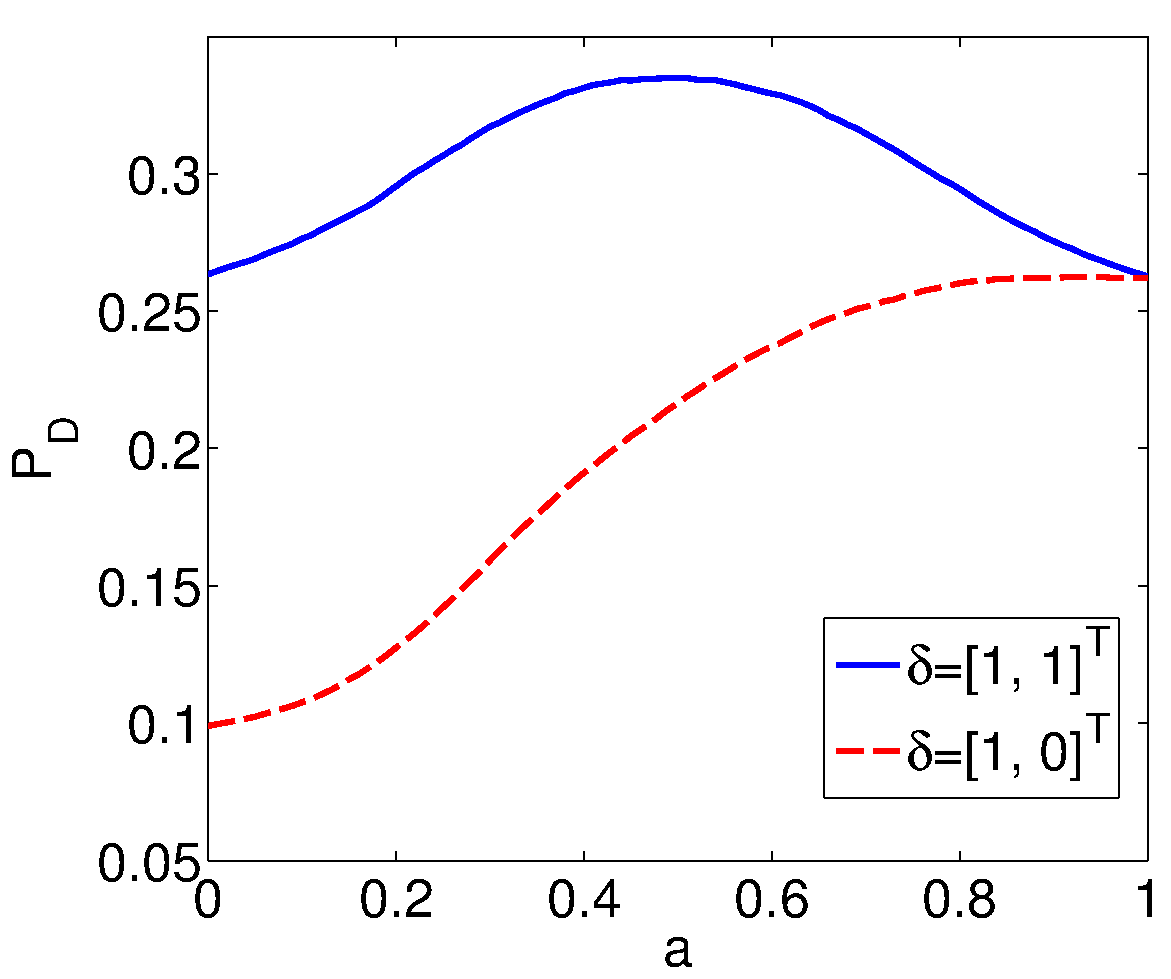
\includegraphics[width=0.45\textwidth]{taes_msd/figures/weights_easy.pdf}
  \label{fig:weights_easy}}
\subfigure[Difficult Optimal Weights]{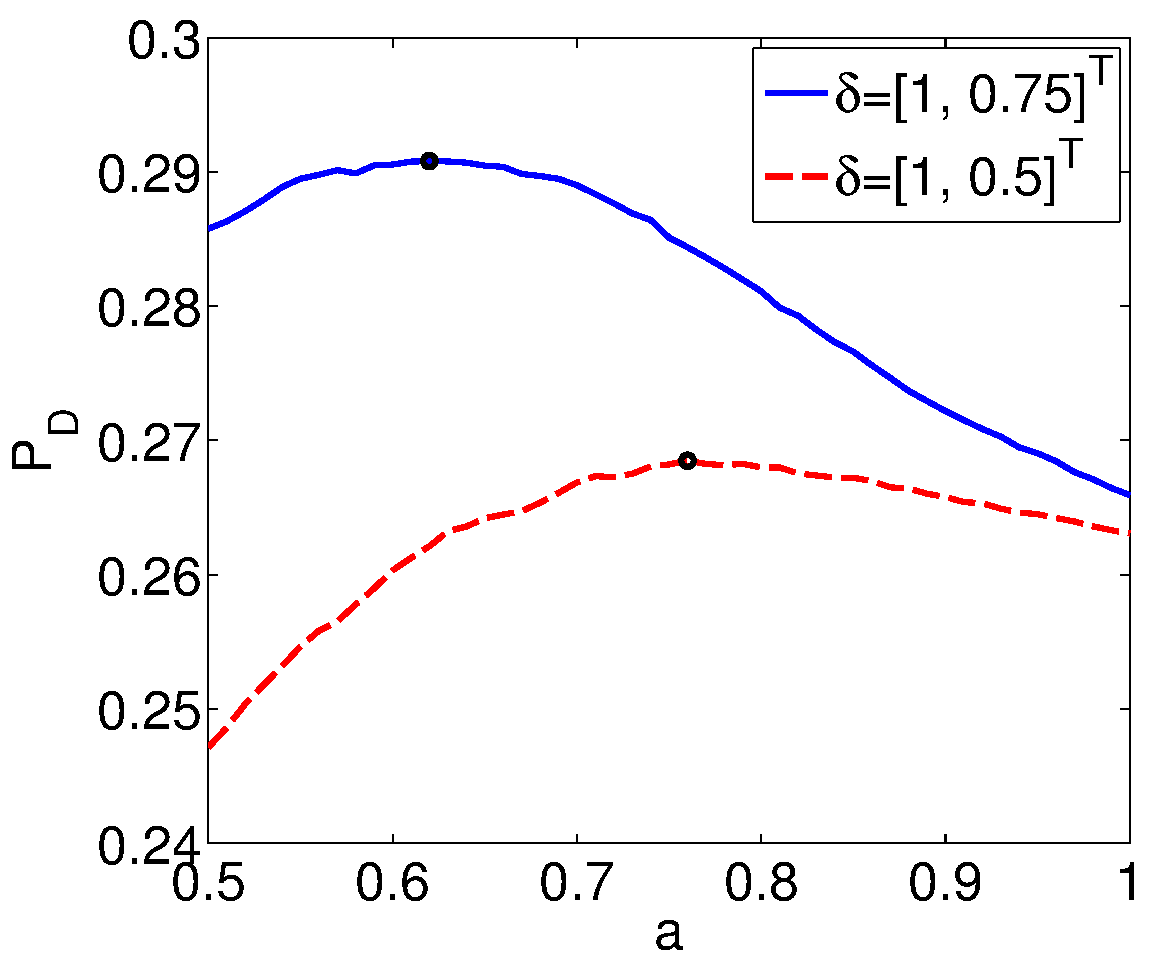
\includegraphics[width=0.45\textwidth]{taes_msd/figures/weights_hard.pdf}
  \label{fig:weights_hard}}
\caption{Empirically achieved probability of detection ($P_D$) as a function of the
  weighting coefficient $a$ for a fixed false alarm rate of $P_F=0.1$. (a) Two detectors,
  one using the deterministic vector $\delta=[1,1]^T$ and the second using
  $\delta=[1,0]^T$.  The first detector achieves its maximum performance around $a=0.5$
  indicating that both components are equally informative. The second detector achieves
  its maximum performance at $a=1$ indicating the second subspace component is not useful
  in detection. (b) Two detectors, one using $\delta=[1, 0.75]^T$ and the other using
  $\delta=[1, 0.5]^T$. The maximum performance of each detector is no longer achieved at
  $a=0.5$ or $a=1$ as the entries of $\delta$ are non-zero and are not equal. The maximum
  performance is indicated by a black circle.}
\label{fig:weighted}
\end{figure}


Figure \ref{fig:weights_hard} considers detectors using $\delta=[1, 0.75]^T$ and $\delta=[1,
0.5]^T$. Both choices place $\delta_1>\delta_2$ so we only consider the regime $a\in[0.5,
1]$, which weights the first component stronger than the second. The maximum performance
of each detector is indicated by a black circle. Unlike the detectors in Figure
\ref{fig:weights_easy}, the maximum $P_D$ is not achieved at $a=0.5$ or $a=1$; both
components are needed to achieve optimal performance. For these choices of $\delta$, the
weighted energy detector is able to achieve a better performance than a standard energy
detector using either one ($a=1$) or both ($a=0.5$) components. Developing an efficient algorithm
to compute these optimal weights is an important extension of the work in this chapter.


%\section{Extension to Missing Data}\label{sec:chpt3:missing}
%\begin{abstract}
%We consider a matched subspace detection problem where a signal vector residing in an unknown low-rank $k$ subspace is to be detected using a subspace estimate obtained from noisy signal-bearing training data with missing entries. The resulting subspace estimate is inaccurate due to limited training data, missing entries, and additive noise. Recent results from random matrix theory (RMT) precisely quantify these subspace estimation errors for the setting where the signal has low coherence. We analytically quantify the ROC performance of the resulting plug-in detector and derive a new detector which explicitly accounts for these subspace estimation errors. The realized increase in performance can be attributed to the new detector only using the $k_\text{eff}\leq k$ ``informative'' signal subspace components. The fraction of observed entries determines $k_\text{eff}$ via a simple relationship that we describe. Detection performance better than random guessing is only achievable when the percent of observed data is above a critical threshold which we explicitly characterize.
%\end{abstract}
%

%\section{Introduction}\label{sec:intro}

%The matched subspace detector (MSD) is a widely used tool in signal processing and machine learning to detect a signal embedded in a low-rank subspace in the presence of additive noise \cite{scharf1994matched,jin2005cfar,mcwhorter2003matched}. The performance of the MSD has been explored when the low-rank signal subspace is known. Scharf and Friedlander \cite{scharf1994matched} consider the MSD when the signal is placed deterministically at an unknown location in a known subspace while McWhorter and Scharf \cite{mcwhorter2003matched} extend this work to allow the signal to be placed randomly with a known (or assumed) distribution in the known subspace.

%There is little work characterizing the performance of the matched subspace detector when the signal subspace is unknown and estimated from data. Recently, we used RMT to quantify the performance of stochastic MSDs in such a setting  \cite{asendorf2011msd}. That work brought into sharp focus the importance of using $k_\text{eff}\leq k$ informative signal subspace components in detector statistics; here $k_{\text{eff}}$ is the effective number of informative components identifiable from limited, noisy data as described in \cite{nadakuditi2008sample}. In this paper, we extend the analysis to the deterministic MSD setting where the training data is noisy \textit{and} has missing entries. The missing entry context is motivated in \cite{balzano2010high} by distributed detection scenarios where it might be prohibitive to collect and transmit only a (randomly chosen) fraction $p$ of the training data entries. Alternately one might think of $1-p \in (0,1)$ as a compression factor as in compressed sensing.

%The main contribution of this paper is a precise quantification of the resulting performance of the MSD. We uncover a phase transition phenomenon by showing that there is a critical fraction, $p_\text{crit}$, which is a simple function of the eigen-SNR, the number of training samples, and the number of sensors, below which detection performance deteriorates to random guessing. Compressing the training dataset below this critical fraction is undesirable.

%The paper is organized as follows. Section \ref{sec:prob stat} formally states the detection problem. Section \ref{sec:rmt} presents pertinent results from RMT. These results are used in Section \ref{sec:derive} to derive a plug-in and random matrix theory MSD and in Section \ref{sec:roc} to derive theoretical ROC curves for each detector. Section \ref{sec:results} validates our analytical predictions, highlights the importance of selecting $k_\text{eff}$ over $k$ subspace components, and demonstrates the effect of missing data. Section \ref{sec:conclusion} presents concluding remarks.

\section{Deterministic Matched Subspace Detectors with Missing Data}\label{sec:chpt3:missing}

We consider the same detection setting as described in Section \ref{sec:msd} using the training
data model in (\ref{eq:taes_train}). However, we only observe a
fraction $p\in(0,1)$ of the entries of our training matrix $Y=[y_1,\dots,y_m]$; $p$ is
independent of $n$ and $m$. Define our observed training data matrix, $\widetilde{Y}$, as
\beq\label{eq:data_model_miss}
\widetilde{Y} = Y\odot M
\eeq
where
\be
 M_{ij} = \begin{cases} 1 & \text{ with probability } \gamma_y\\ 0 & \text{ with
    probability } 1-\gamma_y \end{cases}
\ee
and $\odot$ denotes the Hadamard or element-wise product. Finally we make the following
assumption about our signal subspace, $U$.

\begin{Assum}\label{assum:msd_coher}
In the missing data setting, assume that the columns of $U$ satisfy a `low-coherence'
condition in the following sense: we suppose that there exist 
non-negative constants $\eta$, $C$ independent of $n$, such that for $i=1,\dots,k$ 
\be
\max_i \|u_i\|_\infty \leq \eta\frac{\log^{C}n}{\sqrt{n}}.
\ee
\end{Assum}
We form a signal subspace estimate as in (\ref{eq:param_estims_stoch}), except that we use
our partially observed training matrix $\widetilde{Y}$ to form the sample covariance
matrix $S$ . Call this signal subspace estimate $\widetilde{U}$. 

\subsection{Pertinent Results from RMT}\label{sec:rmt}

By modifying an argument in  \cite{benaych2011singular}, we obtain the following result.
\begin{Th}\label{th:angles}
Assume that $x_i \sim \mathcal{CN}(0,\Sigma^2)$ as in (\ref{eq:taes_train}) and that $U$
in (\ref{eq:taes_train}) obeys the low coherence condition in Assumption
\ref{assum:msd_coher}. Then as $n,m \to \infty$ with $n/m \to c$ we have that
for $i,j = 1, \ldots, k$: 
\begin{equation*}
\begin{aligned}
&|\langle u_i,\widehat{u}_i\rangle|^2\convas
\begin{cases}
1-\dfrac{c\left(1+p\sigma_i^2\right)}{p\sigma_i^2\left(p\sigma_i^2 + c\right)} & \text{ if } \sigma_{i}>\dfrac{c^{1/4}}{\sqrt{p}}\\
0 & \textrm{otherwise}\\
\end{cases}\\
&|\langle u_i,\widehat{u}_j\rangle|^2\convas 0 \qquad \textrm{ for } i \neq j.\\
\end{aligned}.
\end{equation*}
where $\widehat{u}_i$ are the left singular vectors of $\widetilde{Y}$.
\end{Th}

The low coherence condition appears in, for example, \cite{balzano2010high} with the idea
being that the matrix $U \begin{bmatrix} x_{1} & \ldots & x_{m} \end{bmatrix}$ has entries
of about the same magnitude. With the Gaussianity assumption for $x$, all we need is $U$
to have low coherence. Recall that the coherence of a matrix with orthonormal columns is
$\max_{i,j}|U_{i,j}|$. When a matrix is spiky, random sampling of its entries may result
in a loss of information; matrices with low coherence behave better under random sampling
and it is this setting that we focus on in this chapter.

The key insight from Theorem \ref{th:angles} is that only the singular vectors
corresponding to signal singular values above the phase transition
$\frac{c^{1/4}}{\sqrt{p}}$ are \textit{informative}. The fraction of missing entries $p$
regulates this phase transition point as $O(1/\sqrt{p})$. When a signal singular value
drops below this critical threshold, the corresponding singular vector estimate is
essentially noise-like (i.e. $|\langle u_i,\widehat{u}_i\rangle|^2=o_{p}(1)$) and thus
\textit{uninformative}. The term $|\langle u_i,\widehat{u}_i\rangle|^2$ quantifies
mismatch between the estimated and underlying singular vectors; when $p < p_{\text{crit.}}
:=\sqrt{c}/\max_{i}(\sigma_{i}^{2})$ then \textit{all} singular vectors are
uninformative. Intuitively we expect a degradation in the performance of detectors that
utilize subspace components for which $|\langle u_i,\widehat{u}_i\rangle|^2=o_{p}(1)$.  We
refer to the estimate in Theorem \ref{th:angles} as $|\langle
u_i,\widehat{u}_i\rangle|^2_{\text{rmt}}$.

\subsection{Plug-in and RMT Detectors}\label{se:miss_detects}

Using the estimate of our signal subspace, $\widetilde{U}$, formed from our partially
observed training data matrix $\widetilde{Y}$, we define 
\be
\widetilde{w} = \widetilde{U}^Ty
\ee
where $y$ is a testing vector from (\ref{eq:determ_setup}). Note that in this setup, we
don't assume that our testing observation has any missing entries. Following a similar
derivation from Chapter 2 and the previous section, we have our plug-in and RMT test
statistics are
\begin{equation}\label{eq:plugin missing}
\Lambda_{\text{plugin}}(\widetilde{w}) =\widetilde{w}^H\widetilde{w}\sum_{i=1}^k\widetilde{w}_i^2
\end{equation}
\begin{equation}\label{eq:rmt_missing}
\Lambda_{\text{plugin}}(\widetilde{w}) =\widetilde{w}^H\widetilde{w}\sum_{i=1}^{\keff}\widetilde{w}_i^2
\end{equation}
where we define $k_\text{eff}$ as the number of signal singular values above the phase
transition $\frac{c^{1/4}}{\sqrt{p}}$ shown in Theorem \ref{th:angles}. We may use either
test statistic to form a detector of the form 
\begin{equation}\label{eq:opt classifier}
\Lambda(\widetilde{w}) \detgtrless \ln(\eta)
\end{equation}
where $\eta$ satisfies $P(\Lambda(\widetilde{w})>\ln\left(\eta\right)|H_0)=\alpha$.

\subsection{Theoretical ROC Curve Derivation}\label{sec:roc_missing}
A standard way to compare the plug-in and RMT detectors derived in (\ref{eq:plugin missing}) and (\ref{eq:rmt_missing}) respectively is to compute their ROC curves. For a particular statistic $\Lambda(\widetilde{w})$, to compute theoretical ROC curves, we must compute
\begin{equation}\label{eq:target cdf}
\begin{aligned}
&P_D = P(\Lambda(w) > \gamma| w\in H_1)\\
&P_F = P(\Lambda(w) > \gamma| w\in H_0)\\
\end{aligned}
\end{equation}
for $-\infty<\gamma<\infty$. To do this, we explore the conditional CDF under each hypothesis for the statistics (\ref{eq:plugin missing}) and (\ref{eq:rmt_missing}).

This derivation is the same as in Chapter 2 except that we replace $|\langle
u_i,\widehat{u}_i\rangle|_{\text{rmt}}^2$ with the expression in Theorem \ref{th:angles}. 

\section{Simulation Results and Discussion}\label{sec:results}

\begin{figure}[t]
\centering
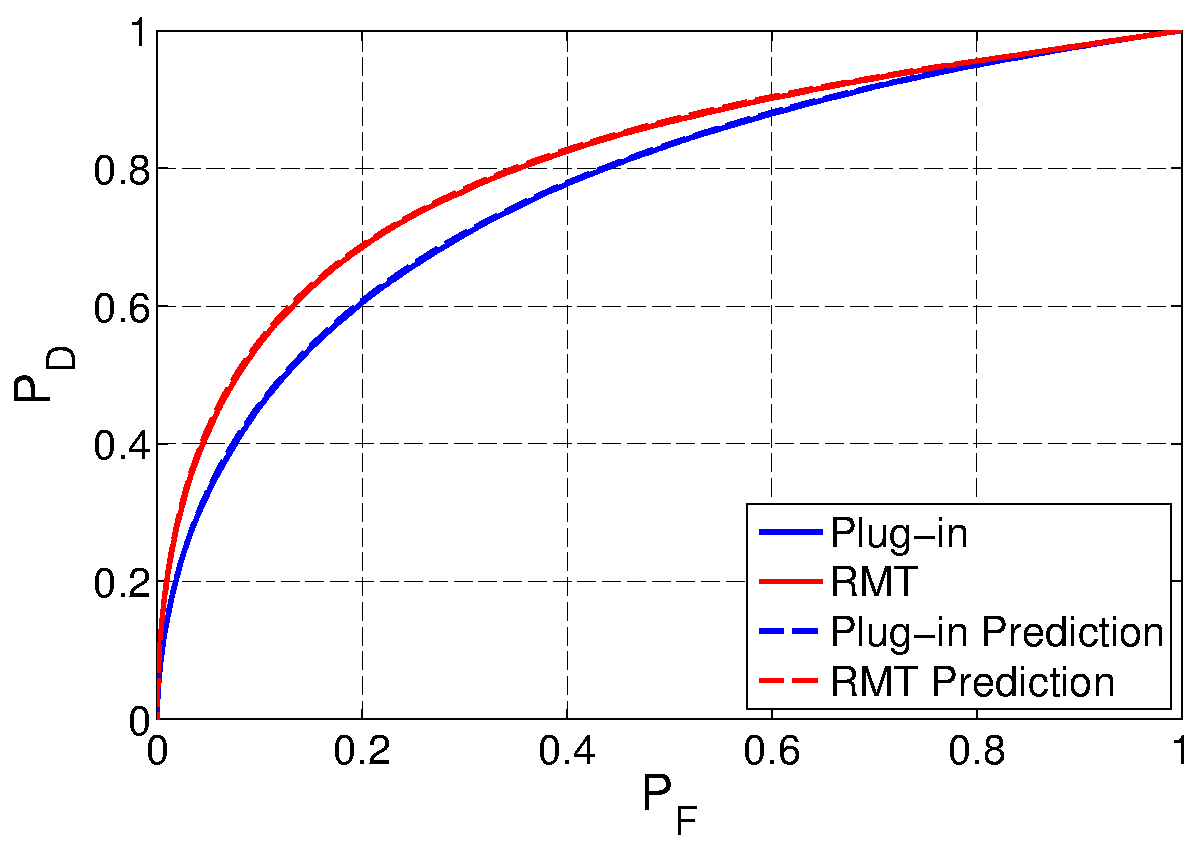
\includegraphics[width=3in]{msd_missing/figures/basic_roc.pdf}
\caption{Empirical and theoretical ROC curves for the plug-in and RMT matched subspace detectors. Empirical ROC curves were simulated with $n=500$, $m=500$, $k=2$, $\Sigma=\diag(3,0.1)$, and $p=0.8$. However, as $\sigma_2$ is below the critical threshold, $k_{\text{eff}} = 1$. The empirical ROC curves were computed using $5000$ test samples and averaged over 25 trials. $x$ was generated randomly for training samples but fixed for test samples. The theoretical ROC curves were obtained using (\ref{eq:roc}). Note the excellent agreement and the performance gain realized by the RMT detector.}\vskip-0.45cm
\label{fig:roc1}
\end{figure}


\subsection{ROC Curves}

We consider a setting where $k_{\text{eff}} = 1 < k = 2$. For this setting, as seen in Figure \ref{fig:roc1}, for any false alarm rate ($P_F$), the RMT detector achieves a higher probability of detection ($P_D$), demonstrating the sub-optimality of the plug-in detector. This is expected because $k_\text{eff}<k$ so that the plug-in detector is employing uninformative subspace components. The theoretical ROC curves in (\ref{eq:roc}) match the empirically generated ROC curves validating the performance predictions of (\ref{eq:roc}) which rely on Theorem \ref{th:angles}.

\subsection{Effect of Missing Data}
Figure \ref{fig:sparsity} examines the performance of each detector as a function of $p$. Again we observe the sub-optimality of the plug-in detector. The theoretical $P_D$ prediction in (\ref{eq:roc}) matches empirically achieved $P_D$ for both detectors. As expected, as $p$ decreases, the achieved probability of detection decreases. We note the presence of a critical $p_{\text{crit.}} : = \sqrt{c}/\max_{i}(\sigma_{i}^{2})$ obtained from Theorem \ref{th:angles}, below which (in the large system limit) we may only achieve $P_D=P_F$; the rounding in Figure \ref{fig:sparsity} is attributed to finite system approximation error.

\begin{figure}[t]
\centering
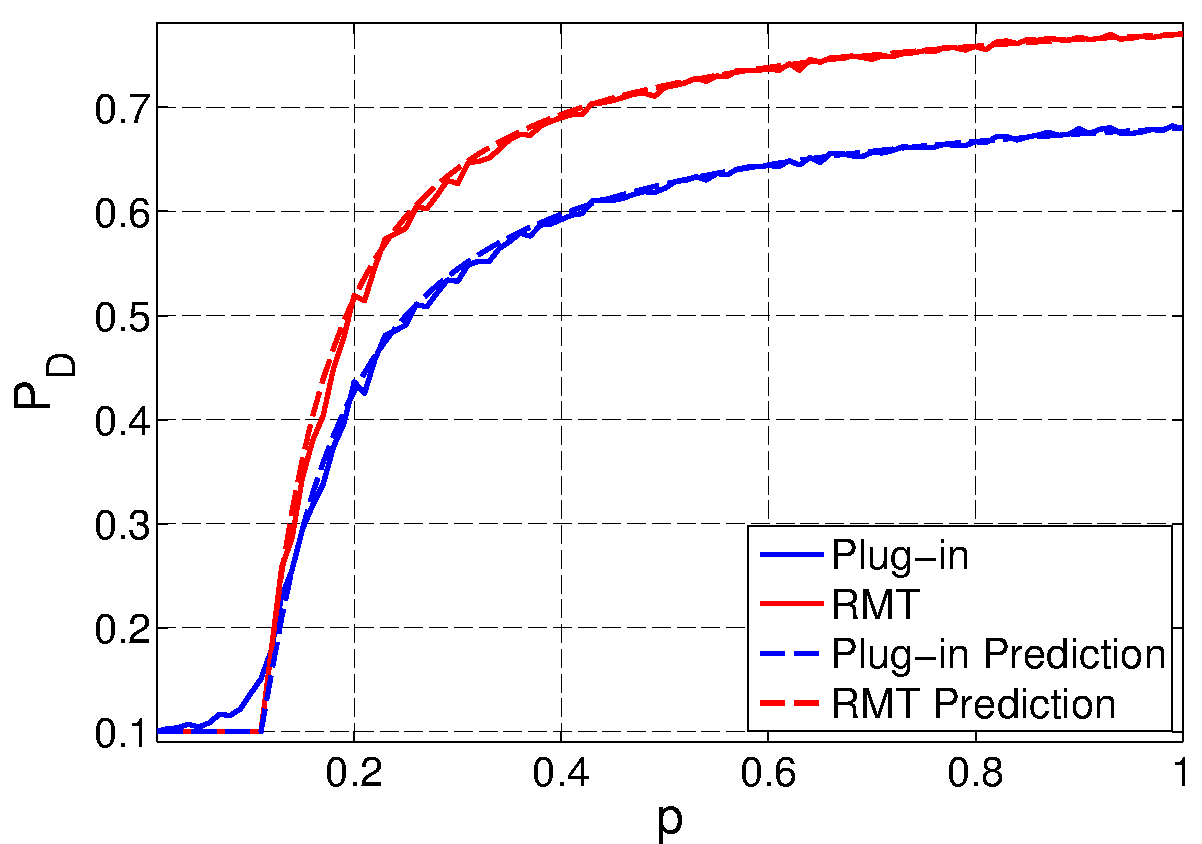
\includegraphics[width=3in]{msd_missing/figures/sparsity.pdf}
\caption{Empirically computed probability of detection, $P_D$, for a fixed probability of false alarm, $P_F=0.1$, for various $p$. Here, $n=1000$, $m=1000$, $k=2$, $\Sigma=\diag(3,0.1)$. $P_D$ was computed using (\ref{eq:roc}) and $x$ was generated as described in Figure \ref{fig:roc1}. For values of $p \leq 1/9$, $k_\text{eff}=0$ and performance degrades to $P_D = P_F +o(1)$ for both detectors. As $p$ increases, $k_\text{eff}=1$ allowing the detectors to achieve better than random guessing performance. When $k_\text{eff}>0$ the plug-in detector is sub-optimal for all values of $p$.}\vskip-0.45cm
\label{fig:sparsity}
\end{figure}





\section{Conclusion}\label{sec:conclusion}
In this paper, we considered a matched subspace detection problem where the low-rank signal subspace is unknown and must be estimated from finite, noisy, signal-bearing training data. We considered both a stochastic and deterministic model for the testing data. The subspace estimate is inaccurate due to finite and noisy training samples and therefore degrades the performance of plug-in detectors compared to an oracle detector. We showed how the ROC performance curve can be derived from the RMT-aided quantification of the subspace estimation accuracy.

Armed with this RMT knowledge, we derived a new RMT detector that only uses the effective number of informative subspace components, $k_\text{eff}$. Plug-in detectors that use the uninformative components will thus incur a performance degradation, relative to the RMT detector. \textcolor{blue}{In settings where a practitioner might play-it-safe and set $\widehat{k}> \widehat{k}_{\text{eff}}$, the performance loss in significant (see Figures \ref{fig:stoch_theory_epsilon} and \ref{fig:determ_theory_epsilon} for a demonstration of how much training data such a play-it-safe plug-in detector would need to match the performance of a $\keff$-tuned RMT detector).} This highlights the importance of robust techniques \cite{nadakuditi2010fundamental,johnstone2001distribution,el2007tracy} for estimating $k_\text{eff}$ in subspace based detection schemes as opposed to estimating $k$, particularly in the regime where $k_{\text{eff}} < k$.  We showed in Tables \ref{table:summary_stoch} and \ref{table:summary_determ} that the distributions of the test statistics could be expressed as a weighted sum of independent chi-squared random variables. The associated ROC curves can then be computed using a saddlepoint approximation.

\textcolor{blue}{The results in this paper can be extended in several directions. We note that the stochastic detector setting assumed normally distributed training and test data. We can extend the analysis to the Gaussian training data but non-Gaussian test vector setting by `integrating-out' the deterministic detector performance curves with respect to the non-Gaussian distribution of the test-vector. Our results relied on characterization of the quantity $\langle u_{j},\widehat{u}_{i}\rangle$.  Thus analogous performance curves can be obtained for any alternate training data models for which this quantity can be analytically quantified. To that end, the results in \cite{benaych2011singular} facilitate such an analysis for a broader class of models including the correlatted Gaussians training data setting. An extension to the missing data setting might follow a similar approach and appears within reach. Aspects related to rate of convergence are open and will be the subject of future work.}



%\bibliographystyle{IEEEtran}
%\bibliography{IEEEabrv,taes_useful.bib}


%\chapter{The performance of deterministic matched subspace detectors when using subspaces estimated from noisy, missing data}\label{sec:ms_missing}
%%\begin{abstract}
%We consider a matched subspace detection problem where a signal vector residing in an unknown low-rank $k$ subspace is to be detected using a subspace estimate obtained from noisy signal-bearing training data with missing entries. The resulting subspace estimate is inaccurate due to limited training data, missing entries, and additive noise. Recent results from random matrix theory (RMT) precisely quantify these subspace estimation errors for the setting where the signal has low coherence. We analytically quantify the ROC performance of the resulting plug-in detector and derive a new detector which explicitly accounts for these subspace estimation errors. The realized increase in performance can be attributed to the new detector only using the $k_\text{eff}\leq k$ ``informative'' signal subspace components. The fraction of observed entries determines $k_\text{eff}$ via a simple relationship that we describe. Detection performance better than random guessing is only achievable when the percent of observed data is above a critical threshold which we explicitly characterize.
%\end{abstract}
%

%\section{Introduction}\label{sec:intro}

%The matched subspace detector (MSD) is a widely used tool in signal processing and machine learning to detect a signal embedded in a low-rank subspace in the presence of additive noise \cite{scharf1994matched,jin2005cfar,mcwhorter2003matched}. The performance of the MSD has been explored when the low-rank signal subspace is known. Scharf and Friedlander \cite{scharf1994matched} consider the MSD when the signal is placed deterministically at an unknown location in a known subspace while McWhorter and Scharf \cite{mcwhorter2003matched} extend this work to allow the signal to be placed randomly with a known (or assumed) distribution in the known subspace.

%There is little work characterizing the performance of the matched subspace detector when the signal subspace is unknown and estimated from data. Recently, we used RMT to quantify the performance of stochastic MSDs in such a setting  \cite{asendorf2011msd}. That work brought into sharp focus the importance of using $k_\text{eff}\leq k$ informative signal subspace components in detector statistics; here $k_{\text{eff}}$ is the effective number of informative components identifiable from limited, noisy data as described in \cite{nadakuditi2008sample}. In this paper, we extend the analysis to the deterministic MSD setting where the training data is noisy \textit{and} has missing entries. The missing entry context is motivated in \cite{balzano2010high} by distributed detection scenarios where it might be prohibitive to collect and transmit only a (randomly chosen) fraction $p$ of the training data entries. Alternately one might think of $1-p \in (0,1)$ as a compression factor as in compressed sensing.

%The main contribution of this paper is a precise quantification of the resulting performance of the MSD. We uncover a phase transition phenomenon by showing that there is a critical fraction, $p_\text{crit}$, which is a simple function of the eigen-SNR, the number of training samples, and the number of sensors, below which detection performance deteriorates to random guessing. Compressing the training dataset below this critical fraction is undesirable.

%The paper is organized as follows. Section \ref{sec:prob stat} formally states the detection problem. Section \ref{sec:rmt} presents pertinent results from RMT. These results are used in Section \ref{sec:derive} to derive a plug-in and random matrix theory MSD and in Section \ref{sec:roc} to derive theoretical ROC curves for each detector. Section \ref{sec:results} validates our analytical predictions, highlights the importance of selecting $k_\text{eff}$ over $k$ subspace components, and demonstrates the effect of missing data. Section \ref{sec:conclusion} presents concluding remarks.

\section{Deterministic Matched Subspace Detectors with Missing Data}\label{sec:chpt3:missing}

We consider the same detection setting as described in Section \ref{sec:msd} using the training
data model in (\ref{eq:taes_train}). However, we only observe a
fraction $p\in(0,1)$ of the entries of our training matrix $Y=[y_1,\dots,y_m]$; $p$ is
independent of $n$ and $m$. Define our observed training data matrix, $\widetilde{Y}$, as
\beq\label{eq:data_model_miss}
\widetilde{Y} = Y\odot M
\eeq
where
\be
 M_{ij} = \begin{cases} 1 & \text{ with probability } \gamma_y\\ 0 & \text{ with
    probability } 1-\gamma_y \end{cases}
\ee
and $\odot$ denotes the Hadamard or element-wise product. Finally we make the following
assumption about our signal subspace, $U$.

\begin{Assum}\label{assum:msd_coher}
In the missing data setting, assume that the columns of $U$ satisfy a `low-coherence'
condition in the following sense: we suppose that there exist 
non-negative constants $\eta$, $C$ independent of $n$, such that for $i=1,\dots,k$ 
\be
\max_i \|u_i\|_\infty \leq \eta\frac{\log^{C}n}{\sqrt{n}}.
\ee
\end{Assum}
We form a signal subspace estimate as in (\ref{eq:param_estims_stoch}), except that we use
our partially observed training matrix $\widetilde{Y}$ to form the sample covariance
matrix $S$ . Call this signal subspace estimate $\widetilde{U}$. 

\subsection{Pertinent Results from RMT}\label{sec:rmt}

By modifying an argument in  \cite{benaych2011singular}, we obtain the following result.
\begin{Th}\label{th:angles}
Assume that $x_i \sim \mathcal{CN}(0,\Sigma^2)$ as in (\ref{eq:taes_train}) and that $U$
in (\ref{eq:taes_train}) obeys the low coherence condition in Assumption
\ref{assum:msd_coher}. Then as $n,m \to \infty$ with $n/m \to c$ we have that
for $i,j = 1, \ldots, k$: 
\begin{equation*}
\begin{aligned}
&|\langle u_i,\widehat{u}_i\rangle|^2\convas
\begin{cases}
1-\dfrac{c\left(1+p\sigma_i^2\right)}{p\sigma_i^2\left(p\sigma_i^2 + c\right)} & \text{ if } \sigma_{i}>\dfrac{c^{1/4}}{\sqrt{p}}\\
0 & \textrm{otherwise}\\
\end{cases}\\
&|\langle u_i,\widehat{u}_j\rangle|^2\convas 0 \qquad \textrm{ for } i \neq j.\\
\end{aligned}.
\end{equation*}
where $\widehat{u}_i$ are the left singular vectors of $\widetilde{Y}$.
\end{Th}

The low coherence condition appears in, for example, \cite{balzano2010high} with the idea
being that the matrix $U \begin{bmatrix} x_{1} & \ldots & x_{m} \end{bmatrix}$ has entries
of about the same magnitude. With the Gaussianity assumption for $x$, all we need is $U$
to have low coherence. Recall that the coherence of a matrix with orthonormal columns is
$\max_{i,j}|U_{i,j}|$. When a matrix is spiky, random sampling of its entries may result
in a loss of information; matrices with low coherence behave better under random sampling
and it is this setting that we focus on in this chapter.

The key insight from Theorem \ref{th:angles} is that only the singular vectors
corresponding to signal singular values above the phase transition
$\frac{c^{1/4}}{\sqrt{p}}$ are \textit{informative}. The fraction of missing entries $p$
regulates this phase transition point as $O(1/\sqrt{p})$. When a signal singular value
drops below this critical threshold, the corresponding singular vector estimate is
essentially noise-like (i.e. $|\langle u_i,\widehat{u}_i\rangle|^2=o_{p}(1)$) and thus
\textit{uninformative}. The term $|\langle u_i,\widehat{u}_i\rangle|^2$ quantifies
mismatch between the estimated and underlying singular vectors; when $p < p_{\text{crit.}}
:=\sqrt{c}/\max_{i}(\sigma_{i}^{2})$ then \textit{all} singular vectors are
uninformative. Intuitively we expect a degradation in the performance of detectors that
utilize subspace components for which $|\langle u_i,\widehat{u}_i\rangle|^2=o_{p}(1)$.  We
refer to the estimate in Theorem \ref{th:angles} as $|\langle
u_i,\widehat{u}_i\rangle|^2_{\text{rmt}}$.

\subsection{Plug-in and RMT Detectors}\label{se:miss_detects}

Using the estimate of our signal subspace, $\widetilde{U}$, formed from our partially
observed training data matrix $\widetilde{Y}$, we define 
\be
\widetilde{w} = \widetilde{U}^Ty
\ee
where $y$ is a testing vector from (\ref{eq:determ_setup}). Note that in this setup, we
don't assume that our testing observation has any missing entries. Following a similar
derivation from Chapter 2 and the previous section, we have our plug-in and RMT test
statistics are
\begin{equation}\label{eq:plugin missing}
\Lambda_{\text{plugin}}(\widetilde{w}) =\widetilde{w}^H\widetilde{w}\sum_{i=1}^k\widetilde{w}_i^2
\end{equation}
\begin{equation}\label{eq:rmt_missing}
\Lambda_{\text{plugin}}(\widetilde{w}) =\widetilde{w}^H\widetilde{w}\sum_{i=1}^{\keff}\widetilde{w}_i^2
\end{equation}
where we define $k_\text{eff}$ as the number of signal singular values above the phase
transition $\frac{c^{1/4}}{\sqrt{p}}$ shown in Theorem \ref{th:angles}. We may use either
test statistic to form a detector of the form 
\begin{equation}\label{eq:opt classifier}
\Lambda(\widetilde{w}) \detgtrless \ln(\eta)
\end{equation}
where $\eta$ satisfies $P(\Lambda(\widetilde{w})>\ln\left(\eta\right)|H_0)=\alpha$.

\subsection{Theoretical ROC Curve Derivation}\label{sec:roc_missing}
A standard way to compare the plug-in and RMT detectors derived in (\ref{eq:plugin missing}) and (\ref{eq:rmt_missing}) respectively is to compute their ROC curves. For a particular statistic $\Lambda(\widetilde{w})$, to compute theoretical ROC curves, we must compute
\begin{equation}\label{eq:target cdf}
\begin{aligned}
&P_D = P(\Lambda(w) > \gamma| w\in H_1)\\
&P_F = P(\Lambda(w) > \gamma| w\in H_0)\\
\end{aligned}
\end{equation}
for $-\infty<\gamma<\infty$. To do this, we explore the conditional CDF under each hypothesis for the statistics (\ref{eq:plugin missing}) and (\ref{eq:rmt_missing}).

This derivation is the same as in Chapter 2 except that we replace $|\langle
u_i,\widehat{u}_i\rangle|_{\text{rmt}}^2$ with the expression in Theorem \ref{th:angles}. 

\section{Simulation Results and Discussion}\label{sec:results}

\begin{figure}[t]
\centering
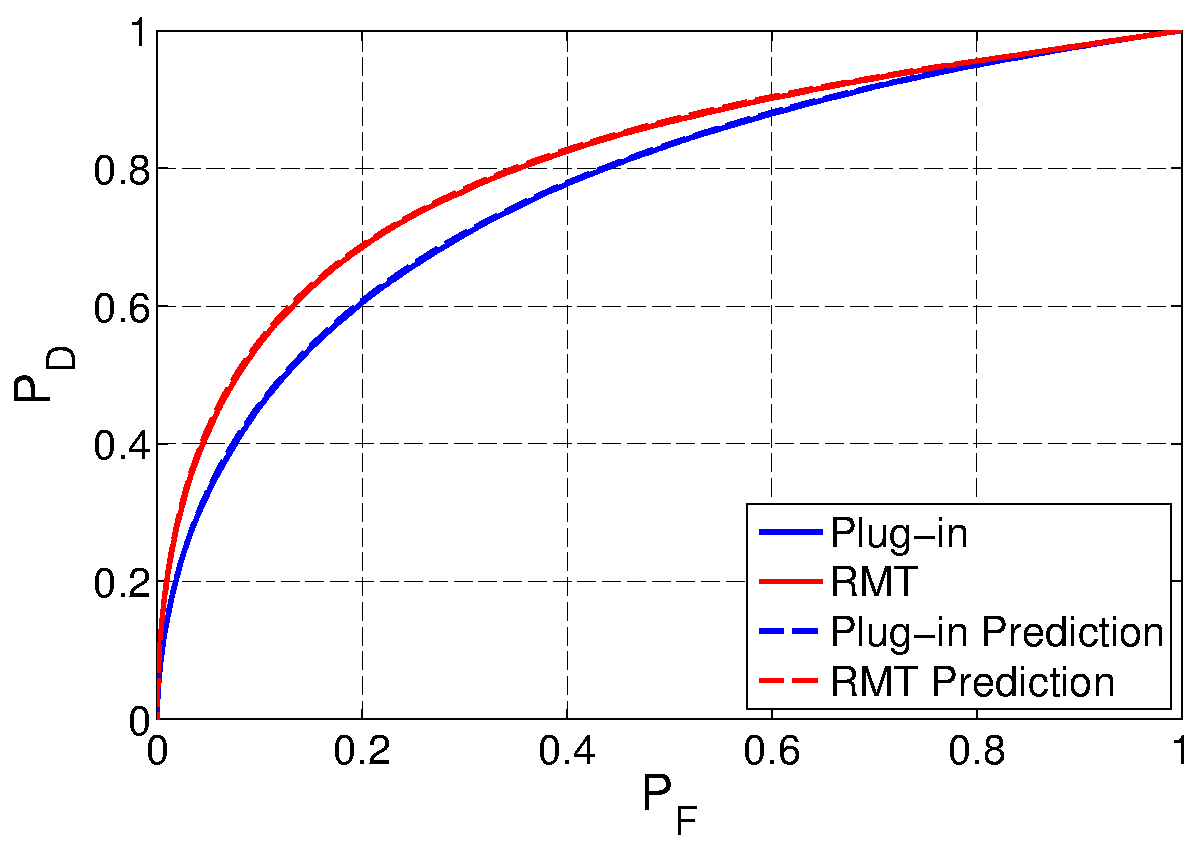
\includegraphics[width=3in]{msd_missing/figures/basic_roc.pdf}
\caption{Empirical and theoretical ROC curves for the plug-in and RMT matched subspace detectors. Empirical ROC curves were simulated with $n=500$, $m=500$, $k=2$, $\Sigma=\diag(3,0.1)$, and $p=0.8$. However, as $\sigma_2$ is below the critical threshold, $k_{\text{eff}} = 1$. The empirical ROC curves were computed using $5000$ test samples and averaged over 25 trials. $x$ was generated randomly for training samples but fixed for test samples. The theoretical ROC curves were obtained using (\ref{eq:roc}). Note the excellent agreement and the performance gain realized by the RMT detector.}\vskip-0.45cm
\label{fig:roc1}
\end{figure}


\subsection{ROC Curves}

We consider a setting where $k_{\text{eff}} = 1 < k = 2$. For this setting, as seen in Figure \ref{fig:roc1}, for any false alarm rate ($P_F$), the RMT detector achieves a higher probability of detection ($P_D$), demonstrating the sub-optimality of the plug-in detector. This is expected because $k_\text{eff}<k$ so that the plug-in detector is employing uninformative subspace components. The theoretical ROC curves in (\ref{eq:roc}) match the empirically generated ROC curves validating the performance predictions of (\ref{eq:roc}) which rely on Theorem \ref{th:angles}.

\subsection{Effect of Missing Data}
Figure \ref{fig:sparsity} examines the performance of each detector as a function of $p$. Again we observe the sub-optimality of the plug-in detector. The theoretical $P_D$ prediction in (\ref{eq:roc}) matches empirically achieved $P_D$ for both detectors. As expected, as $p$ decreases, the achieved probability of detection decreases. We note the presence of a critical $p_{\text{crit.}} : = \sqrt{c}/\max_{i}(\sigma_{i}^{2})$ obtained from Theorem \ref{th:angles}, below which (in the large system limit) we may only achieve $P_D=P_F$; the rounding in Figure \ref{fig:sparsity} is attributed to finite system approximation error.

\begin{figure}[t]
\centering
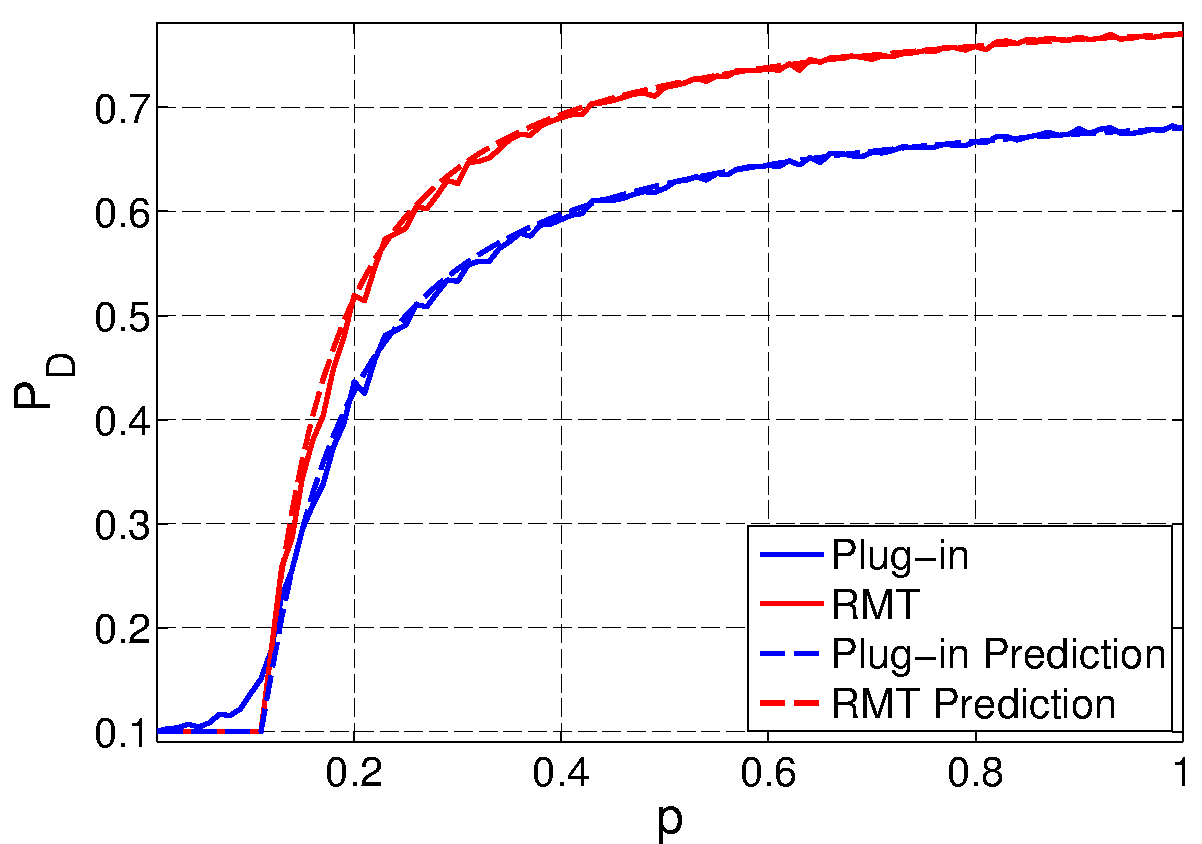
\includegraphics[width=3in]{msd_missing/figures/sparsity.pdf}
\caption{Empirically computed probability of detection, $P_D$, for a fixed probability of false alarm, $P_F=0.1$, for various $p$. Here, $n=1000$, $m=1000$, $k=2$, $\Sigma=\diag(3,0.1)$. $P_D$ was computed using (\ref{eq:roc}) and $x$ was generated as described in Figure \ref{fig:roc1}. For values of $p \leq 1/9$, $k_\text{eff}=0$ and performance degrades to $P_D = P_F +o(1)$ for both detectors. As $p$ increases, $k_\text{eff}=1$ allowing the detectors to achieve better than random guessing performance. When $k_\text{eff}>0$ the plug-in detector is sub-optimal for all values of $p$.}\vskip-0.45cm
\label{fig:sparsity}
\end{figure}






\chapter{Using CCA and ICCA to Detect Correlations in Low-Rank Signal-Plus-Noise Datasets}\label{sec:chpt_cca_det}
%We begin by providing an overview of canonical correlation analysis (CCA). For
completeness and ease of future derivations, we derive the solution for CCA from first
principles. We then give an overview of previous work on CCA in the sample starved regime,
summarizing the results of \cite{pezeshki2004empirical,nadakuditi2011fundamental}. We
conclude by providing new results based on the observations in
\cite{nadakuditi2011fundamental}.

\section{Mathematical Formulation of CCA}\label{sec:cca_form}
Assume that observations $\yI\in\complex^{d_1}$, $\yII\in\complex^{d_2}$
are drawn from two distributions $\yI\sim\mathcal{Y}_1$,
$\yII\sim\mathcal{Y}_2$. Furthermore, assume that the distributions have zero mean,
\textit{i.e.} $\E{\yI}=\E{\yII}=0$. We will use the following notation for the covariance
matrices of the distributions: $\E{\yI\yI^H}=\RI$, $\E{\yII\yII^H}=\RII$,
$\E{\yI\yII^H}=\RIII$.

The goal of CCA is to find a linear transformation for each dataset that maximizes the
correlation between the datasets in the projected spaces. We represent the linear
transformations with the canonical vectors $\xI\in\complex^{d_1}$ and
$\xII\in\complex^{d_2}$ and the projection with the canonical variates $\wI=\xI^H\yI$ and
$\wII=\xII^H\yII$. The objective is to find the canonical vectors $\xI$ and $\xII$ that
maximize the correlation between the canonical variates $\wI$ and $\wII$. Formally, the
optimization problem is
\begin{equation}\label{eq:cca_opt}
  \begin{aligned}
    &\argmax_{\xI,\xII}&&\rho = \E{\wI\wII}\\
    & \text{subject to}&&\E{\wI^2}=1, \E{\wII^2}=1.
  \end{aligned}
\end{equation}
Substituting the expressions for the canonical variates and the correlation matrices, this
optimization problem may be written as
\begin{equation}\label{eq:cca_opt2}
  \begin{aligned}
    &\argmax_{\xI,\xII}&&\rho = \xI^H\RIII\xII\\
    & \text{subject to}&&\xI^H\RI\xI=1, \xII^H\RII\xII=1.
  \end{aligned}
\end{equation}

The Lagrangian used to solve (\ref{eq:cca_opt2}) is
\begin{equation}\label{eq:cca_lagr}
  L(\xI,\xII,\lambda_1,\lambda_2) = \xI^H\RIII\xII - \lambda_1(\xI^H\RI\xI -1) - \lambda_2(\xII^H\RII\xII-1).
\end{equation}
Solving (\ref{eq:cca_opt2}) is achieved by setting the partial derivatives of
(\ref{eq:cca_lagr}) equal to zero. Doing so yields 
\beq\label{eq:cca_partials}\ba
& 0 && = \RIII\xII -2\lambda_1\RI\xI\\
& 0 && = \RIII^H\xI -2\lambda_2\RII\xII.\\
\ea\eeq 
By left multiplying the first equation of (\ref{eq:cca_partials})by $\xI^H$ and
the second equation by $\xII^H$ and using the definitions and constraints in
(\ref{eq:cca_opt2}), 
\beq\label{eq:cca_rho} 
\rho = 2\lambda_1=2\lambda_2.
\eeq 
Therefore, the Lagrange multipliers are equal and the value of the maximum correlation
between the datasets is a multiple of the Lagrange multiplier. Solving one equation in
(\ref{eq:cca_partials}) for $\xII$ and substituting in the other results in the following
eigenvalue system
\cite{nielsen2002multiset,nadakuditi2011fundamental,welling2005kcca,kettenring1971canonical,nielsen1994analysis}
\begin{equation}\label{eq:cca_eigval_sys}
  \RI^{-1}\RIII\RII^{-1}\RIII^H\,\xI = \rho^2\xI
\end{equation}
with the relationship
\beq\label{eq:x2}
\xII=\frac{1}{\rho}\RII^{-1}\RIII^H\,\xI.
\eeq

Solving (\ref{eq:cca_eigval_sys}) for the eigenvector corresponding to the largest
eigenvalue solves (\ref{eq:cca_opt2}). Substituting this eigenvalue/eigenvector pair in
(\ref{eq:x2}) gives the complete solution $\left(\xI,\xII,\rho\right)$ for the transformations
  and maximum correlation between the datasets. Multiple canonical basis vectors may be
  found by recursively finding the next largest eigenvalue and corresponding eigenvector
  in (\ref{eq:cca_eigval_sys}). In many learning applications, it is common to project
  onto multiple canonical basis vectors.

 Using a similarity transform, we can frame the eigen-system in (\ref{eq:cca_eigval_sys})
 as an SVD problem. Define $f = \RI^{1/2}\xI$ and $g=\RII^{1/2}\xII$. Then
 (\ref{eq:cca_eigval_sys}) may be rewritten as
\begin{equation}\label{eq:eigval_sys2}
  \RI^{-1/2}\RIII\RII^{-1}\RIII^H\RI^{-H/2}f = \rho^2f.
\end{equation}
Defining $C=\RI^{-1/2}\RIII\RII^{-H/2}$, (\ref{eq:eigval_sys2}) can be rewritten as
\begin{equation}\label{eq:cca_C_eigval}
  CC^Hf=\rho^2f.
\end{equation}

Clearly, from (\ref{eq:cca_C_eigval}), we may obtain a closed form solution for $f$ and
$\rho$ through the SVD of $C$. Let $FKG^H$ be the SVD of $C$ where
$F=[f_1,\dots,f_{d_1}]$, $K\in\complex^{d_1\times
  d_2}=\diag(k_1,\dots,k_{\min\left(d_1,d_2\right)})$, and $G=[g_1,\dots,g_{d_2}]$. Then the solution
for the canonical vector pair corresponding to the largest canonical correlation is
\beq\label{eq:cca_svd_sol}\ba
&\rho = k_1\\
&\xI = \RI^{-1/2}f_1\\
&\xII = \RII^{-1/2}g_1.\\
\ea\eeq

\section{Empirical CCA}\label{sec:emp_cca}

The above analysis assumes that the covariance matrices $\RI$, $\RII$, and $\RIII$ are all
known. However, in most applications these covariance matrices are unknown and must be
estimated from data. In such an empirical setting, we assume that we are given $n$
observations, or samples, from each dataset $\yI^{(i)}$ and $\yII^{(i)}$ for
$i=1,\dots,n$. We may stack these observations in training data matrices
\be
Y_1=\left[\yI^{(1)},\dots,\yI^{(n)}\right], \text{ and } 
Y_2=\left[\yII^{(1)},\dots,\yII^{(n)}\right].
\ee
Using these training data matrices, the sample covariance matrices are
\beq\label{eq:scm}\ba
&\RIhat = \frac{1}{n} Y_1Y_1^H\\
&\RIIhat = \frac{1}{n} Y_2Y_2^H\\
&\RIIIhat = \frac{1}{n} Y_1Y_2^H.\\
\ea\eeq
We may then substitute these covariance matrix estimates in the expression for $C$,
resulting in the estimator
\beq\label{eq:cca_Chat}
\widehat{C} = \RIhat^{-1/2}\RIIIhat\RIIhat^{-1/2}.
\eeq
Defining $\widehat{C} =\widehat{F}\widehat{K}\widehat{G}^H$ as the SVD of $\widehat{C}$,
the solution to empirical CCA is
\beq\label{eq:cca_svd_sol}\ba
&\widehat{\rho} = \widehat{k}_1\\
&\xIhat = \RIhat^{-1/2}\,\widehat{f}_1\\
&\xIIhat = \RIIhat^{-1/2}\,\widehat{g}_1.\\
\ea\eeq

\section{Performance of Empirical CCA}

Here, we present the relevant works that explore the performance of empirical CCA and
demonstrate how they provide insight to the data fusion questions posed herein. First, we
note that to construct $\widehat{C}$ in (\ref{eq:cca_Chat}) we must invert $\RIhat$ and
$\RIIhat$. However, if the number of samples $n$ is less than either of the data
dimensions $d_1$ or $d_2$, then the sample covariances are not invertible. In this case, a
regularized version of CCA is often employed. We discuss this in depth in Chapter
\ref{sec:rcca}.

\subsection{Performance Breakdown When $n<d_1+d_2$}
Pezeshki et al. analyze the performance of empirical CCA in the sample poor regime when
$n<d_1+d_2$ in \cite{pezeshki2004empirical}. In particular, they show that in this regime,
empirical CCA breaks down completely; the leading singular value of $\widehat{C}$ is 
deterministically 1. Below we provide a different proof of this result.

Let $Y_1 = U_1\Sigma_1 V_1^H$ and $Y_2=U_2\Sigma_2V_2^H$ be the data SVDs of our training
data matrix. Using this notation, 
\beq\label{eq:cca_chat_svd}\ba
& \widehat{C} &&= \RIhat^{-1/2}\RIIIhat\RIIhat^{-1/2}\\
&&&  = \left(Y_1Y_1^H\right)^{-1/2}Y_1Y_2^H\left(Y_2Y_2^H\right)^{-1/2} \\
&&& = \left(U_1\Sigma_1\Sigma_1^HU_1^H\right)^{-1/2}U_1
\Sigma_1V_1^HV_2\Sigma_2^HU_2^H\left(U_2\Sigma\Sigma_2\Sigma_2^H\right)^{-1/2}\\
&&& = U_1 I_{d_1\times n}V_1^HV_2I_{n\times d_2}U_2^H\\
\ea\eeq
Therefore, we can conclude that since $U_1$ and $U_2$ are unitary matrices,
\be \widehat{\rho} = \widehat{k}_1 = \sigma_1\left(\widehat{C}\right) =
\sigma_1\left(\bar{V}_1^H \bar{V}_2\right) 
\ee
where $\bar{V}_1=V(:,1:\min\left(d_1,n\right))$, $\bar{V}_2 =
V(:,1:\min\left(d_2,n\right))$, and $\sigma(\cdot)$ returns the largest singular value of
the provided matrix. These (possibly) trimmed matrices have orthonormal columns and thus
form a basis for a subspace. Consider the case when $n<d_1+d_2$. If $n<d_1$ or $n<d_2$,
then either $\bar{V}_1$ or $\bar{V}_2$ is a unitary matrix and so
$\sigma_1\left(\bar{V}_1^H\bar{V}_2\right)=1$ deterministically. In the case when
$\max\left(d_1,d_2\right)<n<d_1+d_2$, $\bar{V}_1$ is a dim-$d_1$ subspace of $\complex^n$ and
$\bar{V}_2$ is a dim-$d_2$ subspace of $\complex^n$. However, because $n<d_1+d_2$, these
subspaces are \textit{guaranteed} to intersect. Let $v$ be the shared basis vector of the
subspaces defined by $\bar{V}_1$ and $\bar{V}_2$. Therefore, we can express these
subspaces using the bases $\bar{V}_1=\left[v\,\, v^{\perp}_{\bar{V}_1}\right]$ and
$\bar{V}_2 = \left[v\,\,  v^{\perp}_{\bar{V}_2}\right]$. Therefore
\be
\bar{V}_1^H\bar{V}_2 = \left[\begin{array}{c}v^H
    \\v^{H\perp}_{\bar{V}_1}\end{array}\right]\left[v \,\,
  v^{\perp}_{\bar{V}_2}\right] = \left[\begin{array}{cc}1 & 0^H \\ 0 &
    v^{H\perp}_{\bar{V}_1}v^{\perp}_{\bar{V}_2}\end{array}\right]. 
\ee
This matrix clearly has a largest singular value of 1.

Therefore, when $n<d_1+d_2$,
$\widehat{\rho}=\widehat{k}_1=\sigma_1\left(\widehat{C}\right)=1$ deterministically. This
is an extremely undesirable property of empirical CCA. When $\widehat{\rho}=1$, it implies
that the canonical vectors provide a transformations that result is perfect (colinear)
correlated canonical variates. This property holds for all distributions and any possible
data matrices $Y_1$ and $Y_2$ even if the datasets contain no correlated signals.

\subsection{Simulation Results}

We now demonstrate this phenomena through a series of simulations. While some of these
results reproduce previous work, they are needed to form a basis for comparison to
new algorithms. In this setup, we consider two cases. In the first, both datasets are
simply Gaussian noise. In the second, each dataset contains a noisy low-rank signal that is
correlated with the other dataset. The data model for this setup is

\beq\label{eq:cca_data_model1}\ba
\text{Noise:}\begin{cases}
\yI^{(i)}=\mathcal{N}\left(0,I_{d_1}\right) & \\
\yII^{(i)}=\mathcal{N}\left(0,I_{d_2}\right) & \\
\end{cases}
\text{Signal:}\begin{cases}
\yI^{(i)}=\sigma u_1 z_1^{(i)} + \mathcal{N}\left(0,I_{d_1}\right) & \\
\yII^{(i)}=\sigma u_2 z_2^{(i)} + \mathcal{N}\left(0,I_{d_2}\right) & \\
\end{cases}
\ea\eeq
where $u_1\in\complex^{d_1}$ and $u_2\in\complex^{d_2}$ are unit norm signal
vectors, $\sigma>0$ is a SNR, and 
\be 
z^{(i)}=\left[\begin{array}{c}z_1^{(i)} \\  z_2^{(i)}\end{array}\right]\sim
\mathcal{N}\left(0,\left[\begin{array}{cc} 1 & \rho \\ \rho & 1\end{array}\right]\right).
\ee 
All additive Gaussian noise terms are independent. We note that in this setup the SNR,
$\sigma$, is the same for both datasets. This would usually not be the case and we could
run these simulations using a $\sigma$ unique to each dataset, however, we wish to reduce
the number of parameters in the simulation.

For $i=1,\dots,n$ we produce $n$ samples for each dataset under both the signal and noise
model in (\ref{eq:cca_data_model1}), resulting in four datasets $Y_1^{\text{noise}}$,
$Y_2^{\text{noise}}$, $Y_1^{\text{signal}}$, and $Y_2^{\text{signal}}$. Using the data
SVDs of $Y_1^{\text{noise}}$ and $Y_2^{\text{noise}}$ we form $\widehat{C}^{\text{noise}}$
as defined in (\ref{eq:cca_chat_svd}) and $Y_1^{\text{signal}}$ and $Y_2^{\text{signal}}$
to similarly form $\widehat{C}^{\text{signal}}$. We then take the leading singular value
of $\widehat{C}^{\text{noise}}$ and $\widehat{C}^{\text{signal}}$, resulting in two top
singular values, $\widehat{\rho}^{\text{noise}}$ and $\widehat{\rho}^{\text{signal}}$,
representing the maximum correlation in the noise datasets and the maximum correlation in
the signal datasets. This is repeated for multiple trials, where each trial generates new
datasets using different signal vectors $u_1$ and $u_2$, new $z$, and new additive
noise. This gives an empirical distribution of $\widehat{\rho}^{\text{noise}}$ and
$\widehat{\rho}^{\text{signal}}$ formed from noisy datasets and signal bearing
datasets. Figure \ref{fig:cca_errorbars} plots these empirical distributions, sweeping
over the number of training samples in each dataset for two values of $\sigma$.

\begin{figure}[h!]
  \centering
  \subfigure[$\sigma=0$ dB]{
    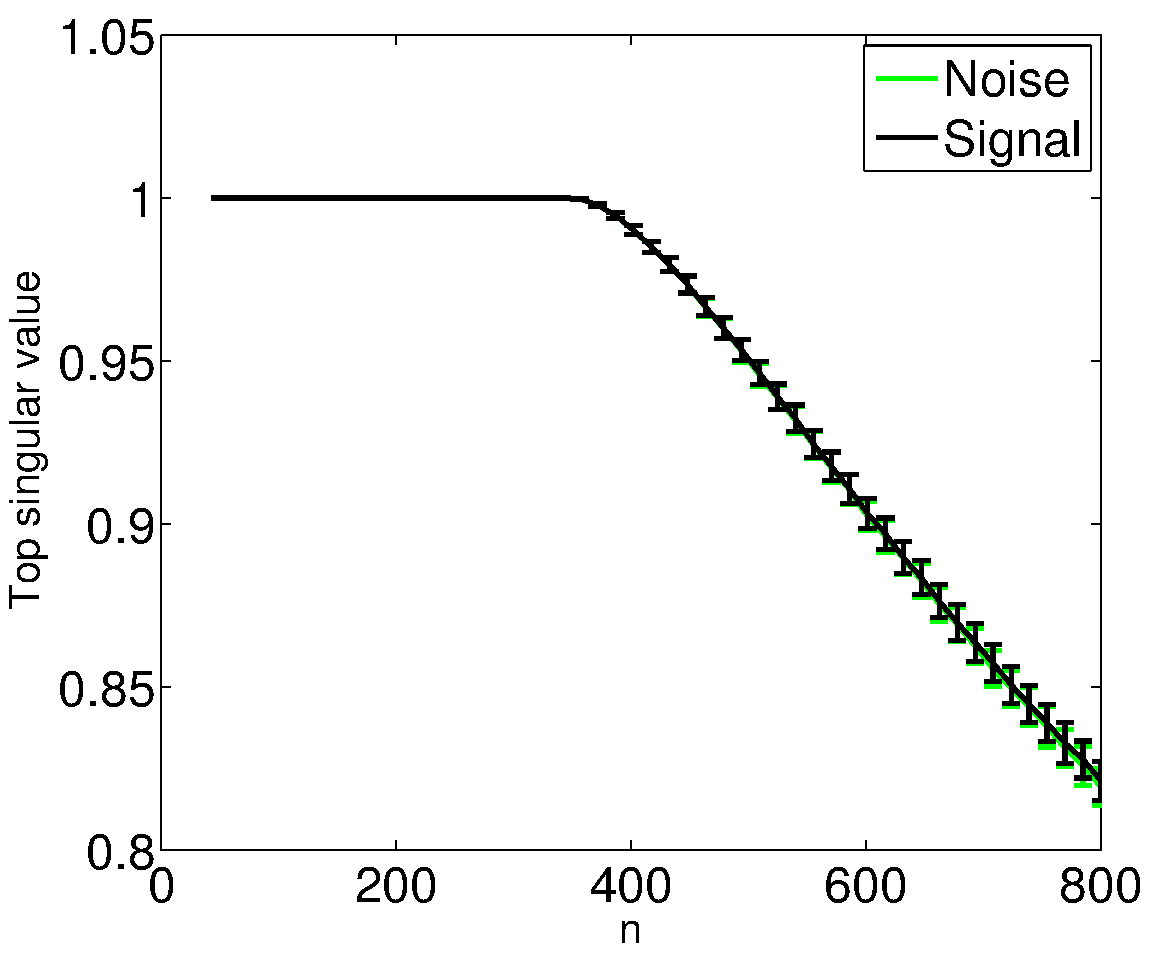
\includegraphics[width=\figwidth]{figures/cca_errorbars_low.pdf}
    \label{fig:cca_errorbars_low_snr}
  }
  \subfigure[$\sigma=3$ dB]{
    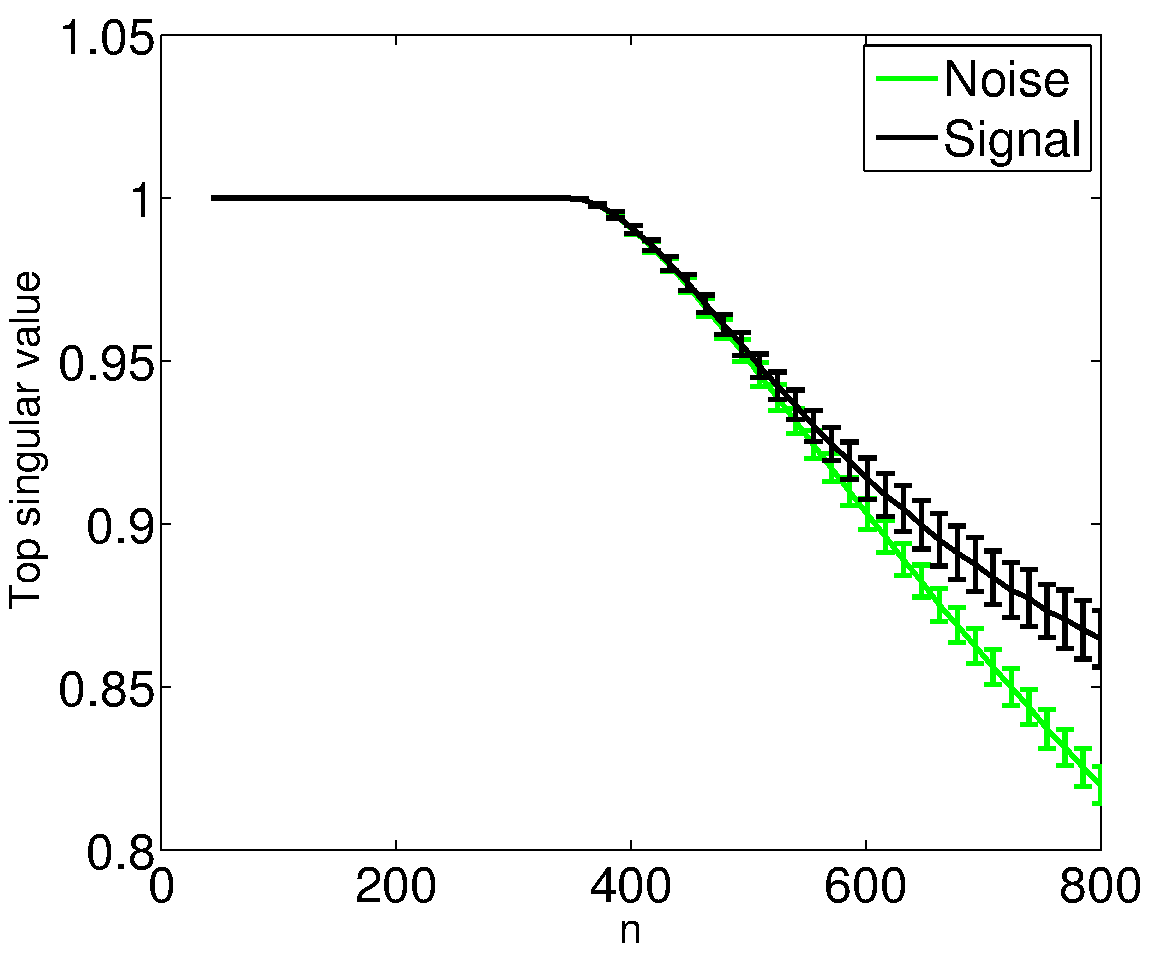
\includegraphics[width=\figwidth]{figures/cca_errorbars_high.pdf}
    \label{fig:cca_errorbars_high_snr}
  }
  \caption{Empirical distribution of the top singular value of $\widehat{C}$ in
    (\ref{eq:cca_chat_svd}) for both noise and signal data models in
    (\ref{eq:cca_data_model1}). Simulations were conducted using $d_1=200$, $d_2=150$, and
    $\rho=0.9$. The top singular value was computed for 500 trials. The mean top singular
    value is plotted with $\pm$ one standard deviation errorbars. }
  \label{fig:cca_errorbars}
\end{figure}

Figure \ref{fig:cca_errorbars} highlights the phenomena presented in
\cite{pezeshki2004empirical}. For $n<350=d_1+d_2$, $\widehat{\rho}$ is identically 1 for
both the noise and signal datasets and for both values of $\sigma$. In Figure
\ref{fig:cca_errorbars_low_snr}, the value of $\sigma$ is small enough so that even when
there are many samples present, the empirical distribution of
$\widehat{\rho}^{\text{noise}}$ follows that of $\widehat{\rho}^{\text{signal}}$. However,
when $\sigma$ is larger, as in Figure \ref{fig:cca_errorbars_high_snr}, the distributions
separate when given enough samples. A natural question to ask is ``Are these distributions
different?'' If the answer is no, then the correlation estimate returned by CCA is
useless, being unable to discern if the correlated datasets contain signal or are simply
noise. Next we reproduce the results of \cite{nadakuditi2011fundamental}, using the
two-sided Kolmorgorov-Smirnov (KS) to determine if the distributions are indeed
different. Figure \ref{fig:cca_ks_heatmap} plots the KS statistic for multiple values of
$\sigma$ and $n$.

\begin{figure}
  \centering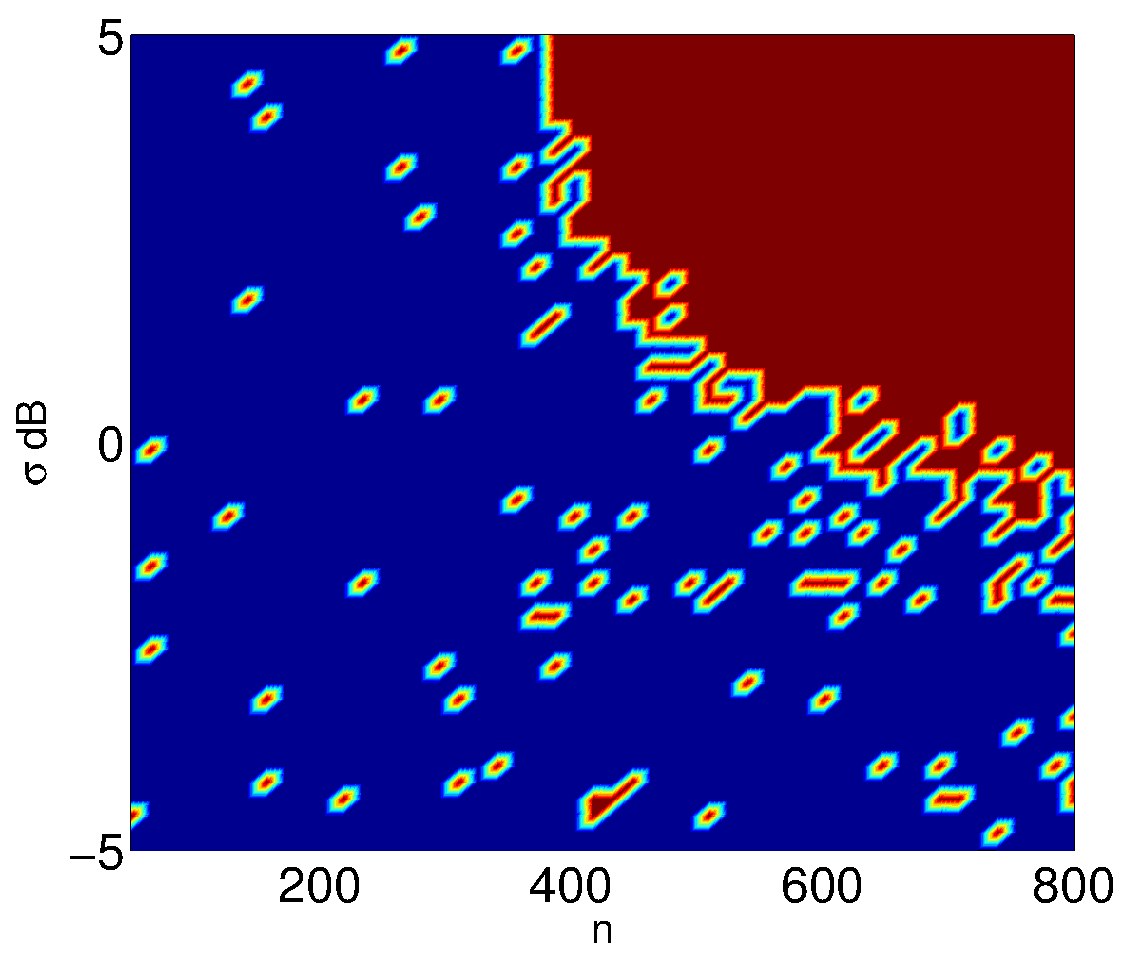
\includegraphics[width=\figwidth]{figures/cca_ks_heatmap.pdf}
  \caption{Two-sided KS statistic between the empirical distributions of the leading
    singular value of $\widehat{C}$ in (\ref{eq:cca_chat_svd}) formed from training data
    generated from the noise and signal data models in (\ref{eq:cca_data_model1}).
    Simulations were conducted using $d_1=200$, $d_2=150$, $\rho=0.9$, 500 trials, and a
    significance level of $\alpha=0.95$ for the KS test. A value of 1 indicates the
    distributions are statistically different while a value of 0 indicates the
    distributions are statistically identical.}
  \label{fig:cca_ks_heatmap}
\end{figure}

This result confirms the result in \cite{nadakuditi2011fundamental}. Two important
consequences follow from Figure \ref{fig:cca_ks_heatmap}. First, it confirms that when
$n<d_1+d_2$ CCA fails to provide meaningful correlation estimates. No matter how large the
value of $\sigma$, CCA will always return a correlation estimate of 1 for any dataset it
is provided. In this sample starved regime, CCA cannot reliably detect the presence of a
signal given two correlated datasets. Second, given $n>d_1+d_2$ samples, there is a
threshold dependent on $n$ such that when $\sigma$ is large enough, the noise and signal
distributions are statistically different and when $\sigma$ is too small, the noise and
signal distributions are statistically identical. The KS statistic determines if the
distributions are statistically distinguishable but gives no insight into \textit{how}
indistinguishable the distributions are. To explore this, we consider constructing a
na\"{\i}ve detector based on the top singular value of $\widehat{C}$. We may construct an
empirical ROC curve of such a detector using the empirical distributions of
$\widehat{\rho}^{\text{noise}}$ and $\widehat{\rho}^{\text{signal}}$. The area under the
ROC curve (AUC) is a measure of the detection ability of such a detector, with 1 being
perfect detection and 0.5 being random guessing. Figure \ref{fig:cca_auc_heatmap} plots
the empirical AUC for such a detector given the empirical distributions for the top
singular value of $\widehat{C}$ under both the noise and signal model.

\begin{figure}
  \centering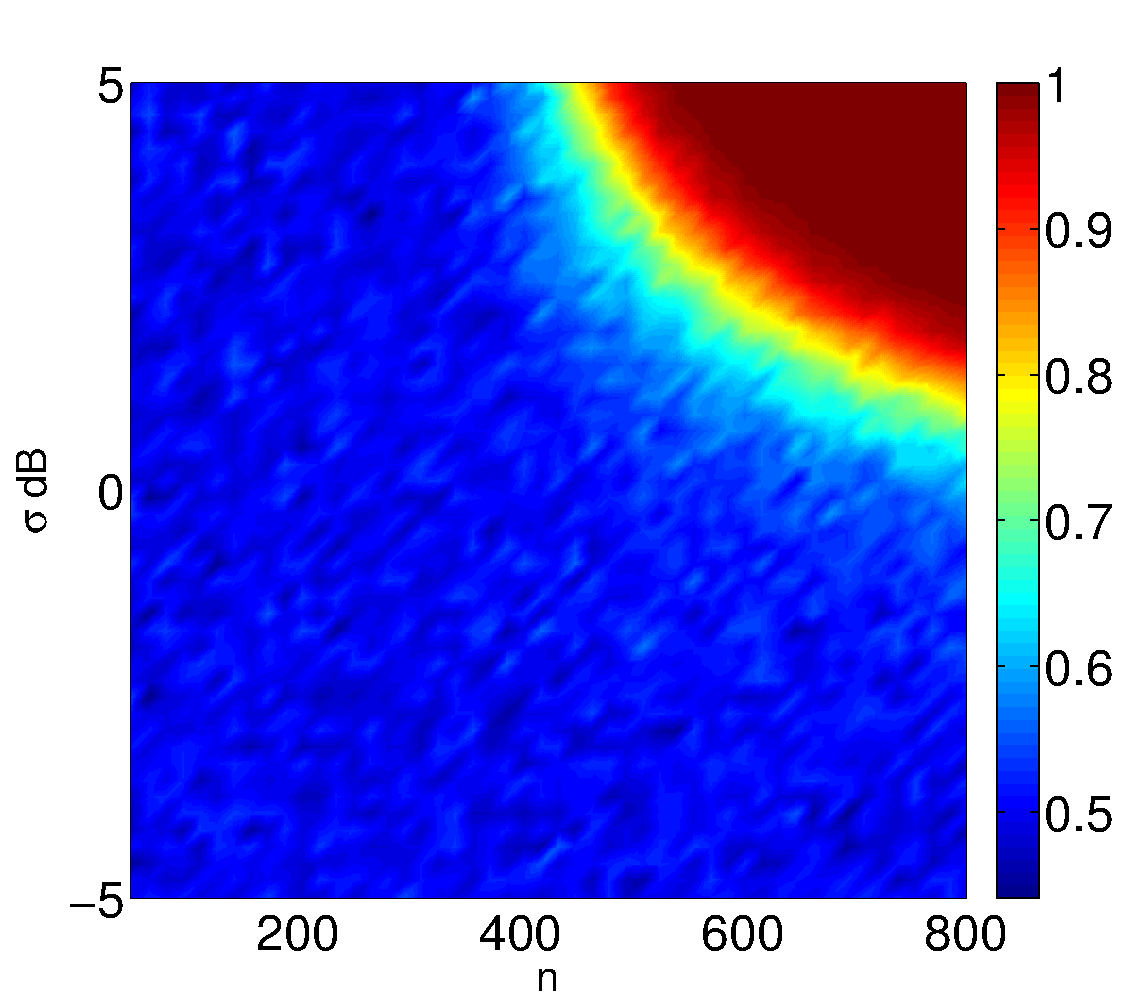
\includegraphics[width=\figwidth]{figures/cca_auc_heatmap.pdf}
  \caption{AUC for a detector based on the top singular value of $\widehat{C}$ in
    (\ref{eq:cca_chat_svd}) to detect the noise and signal data models in
    (\ref{eq:cca_data_model1}). Simulations were conducted using $d_1=200$, $d_2=150$, 500
    trials, and $\rho=0.9$.}
  \label{fig:cca_auc_heatmap}
\end{figure}

This is a new result. While the AUC heatmap in Figure \ref{fig:cca_auc_heatmap} closely
resembles the KS statistic heatmap in Figure \ref{fig:cca_ks_heatmap}, it also provides
information on how far the distributions are separated. When the distributions are
entirely separated, perfect detection is possible, resulting in an AUC of 1. This occurs
for large values of $n$ and $\sigma$. The AUC plot also confirms that when $n<d_1+d_2$,
CCA cannot statistically detect signals given correlated datasets. In fact, a large
portion of the parameter sweep of $n$ and $\sigma$ results in CCA failing.

The breakdown point when $n<d_1+d_2$ is an extremely undesirable property of CCA. In the
low-sample, high dimensional regime, it results in CCA being unable to detect the presence
of a signal given correlated datasets. We demonstrated through numerical simulation that
in this regime the distribution of the leading singular value of noise only datasets is
identical to that of datasets generated with correlated signal. However, using results
from random matrix theory, it is possible to avoid this undesirable performance loss.

\section{Informative CCA (ICCA)}

In \cite{nadakuditi2011fundamental}, Nadakuditi uses recent results from random matrix
theory to derive an informative version of CCA that we will call here informative CCA
(ICCA). Recalling the data SVDs $Y_1=U_1\Sigma_1V_1^H$ and $Y_2=U_2\Sigma_2V_2^H$, random
matrix theory provides the important insight that not all of the right singular vectors
are informative. In particular the following proposition is repeated from
\cite{nadakuditi2011fundamental} for here for reference. Let $z_1=
\left[z_1^{(1)},\dots,z_1^{(n)}\right]^H$ be the correlated signal vector in the first
dataset. 
\begin{prop}\label{prop:raj}
  As $d_1$, $n\to\infty$ with $d_1/n\to c_1$,
  \be
  \left| \left\langle \frac{z_1}{\|z_1\|_2}, V_1(:,1)\right\rangle\right|\convas\begin{cases}
    \varphi_1 & \text{if } \sigma > c_1^{1/4}\\
    0 & \text{otherwise}\\
  \end{cases}, 
  \ee 
  where $\varphi_1:=\sqrt{1 -
    \left(c_1+\sigma^2\right)/\left(\sigma^2\left(\sigma^2+1\right)\right)}$
  \cite{nadakuditi2011fundamental}.
\end{prop}
The analogous theorem holds for the second dataset. The notation $V_1(:,1)$ denotes the
first column of $V_1$. This proposition tells us that there is a critical SNR
$\sigma_{\text{crit}}=\left(\frac{d_1}{n}\right)^{1/4}$ such that if
$\sigma>\sigma_{\text{cirt}}$ the first column of $V_1$ is informative and contains a
portion of the correlated signal $z_1$. However, if $\sigma<\sigma_{\text{crit}}$ the
first column of $V_1$ is uninformative and contains no correlated signal. Such
uninformative components should not be used in CCA as they will degrade its
performance. Following \cite{nadakuditi2011fundamental}, we define the trimmed data
matrices as 
\be\ba
& \widetilde{U}_1 = U(:,1:r_1) && \widetilde{V}_1 = V(:,1:r_1)\\
& \widetilde{U}_2 = U(:,1:r_2) && \widetilde{V}_2 = V(:,1:r_2)\\
\ea\ee 
where $r_1$ and $r_2$ are the number of informative components in the first
and second datasets, respectively.Using these trimmed data matrices, we form the matrix
used for ICCA,
\beq\label{eq:icca_chat}
  \widetilde{C} = \widetilde{U}_1\widetilde{V}_1^H\widetilde{V}_2\widetilde{U}_2^H.
\eeq
Let $\widetilde{C} = \widetilde{F}\widetilde{K}\widetilde{G}^H$ be the SVD of this
matrix. ICCA returns the following informative correlation estimate and canonical vectors
\begin{equation}\label{eq:icca_rho}
\ba
&\widetilde{\rho} &&= \widetilde{k}_1\\
&\widetilde{x}_1 &&= \RIhat^{-1/2}\widetilde{f}_1\\
&\widetilde{x}_2 &&= \RIIhat^{-1/2}\widetilde{g}_1\\
\ea
\end{equation}
We next demonstrate that the correlation estimate returned by ICCA is superior to that
returned by CCA. 

\subsection{Simulation results}

We use the same simulation setup as in the CCA analysis, generating $n$ samples for each
dataset under both the noise and signal model in (\ref{eq:cca_data_model1}). Instead, of
using the estimate $\widehat{C}$, we form the estimates $\widetilde{C}^{\text{noise}}$ and
$\widetilde{C}^{\text{signal}}$ as in (\ref{eq:icca_chat}). First we explore the
distributions of the top singular value, $\widetilde{\rho}^{\text{noise}}$ and
$\widetilde{\rho}^{\text{signal}}$ of these matrices in Figure \ref{fig:icca_errorbars}.

\begin{figure}[h!]
  \centering
  \subfigure[$\sigma=0$ dB]{
    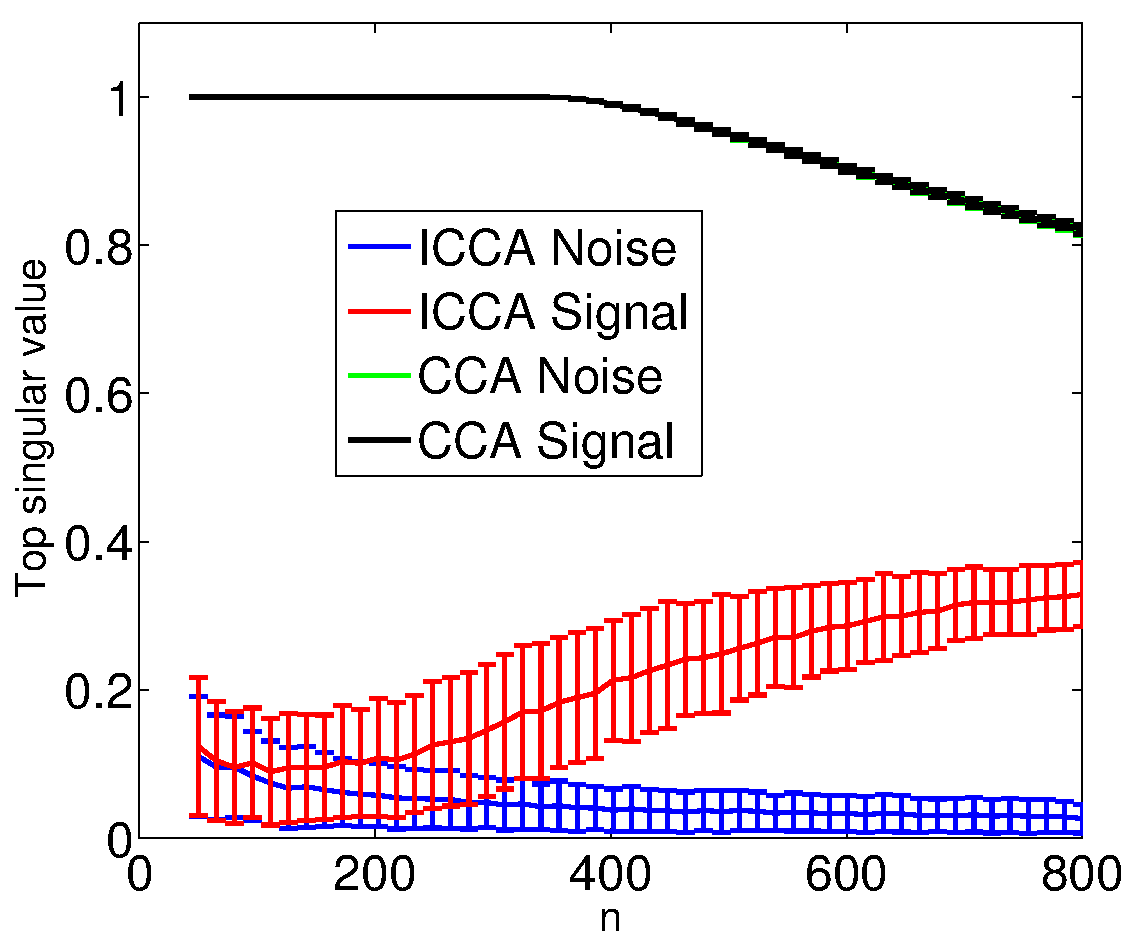
\includegraphics[width=\figwidth]{figures/icca_errorbars_low.pdf}
    \label{fig:icca_errorbars_low_snr}
  }
  \subfigure[$\sigma=3$ dB]{
    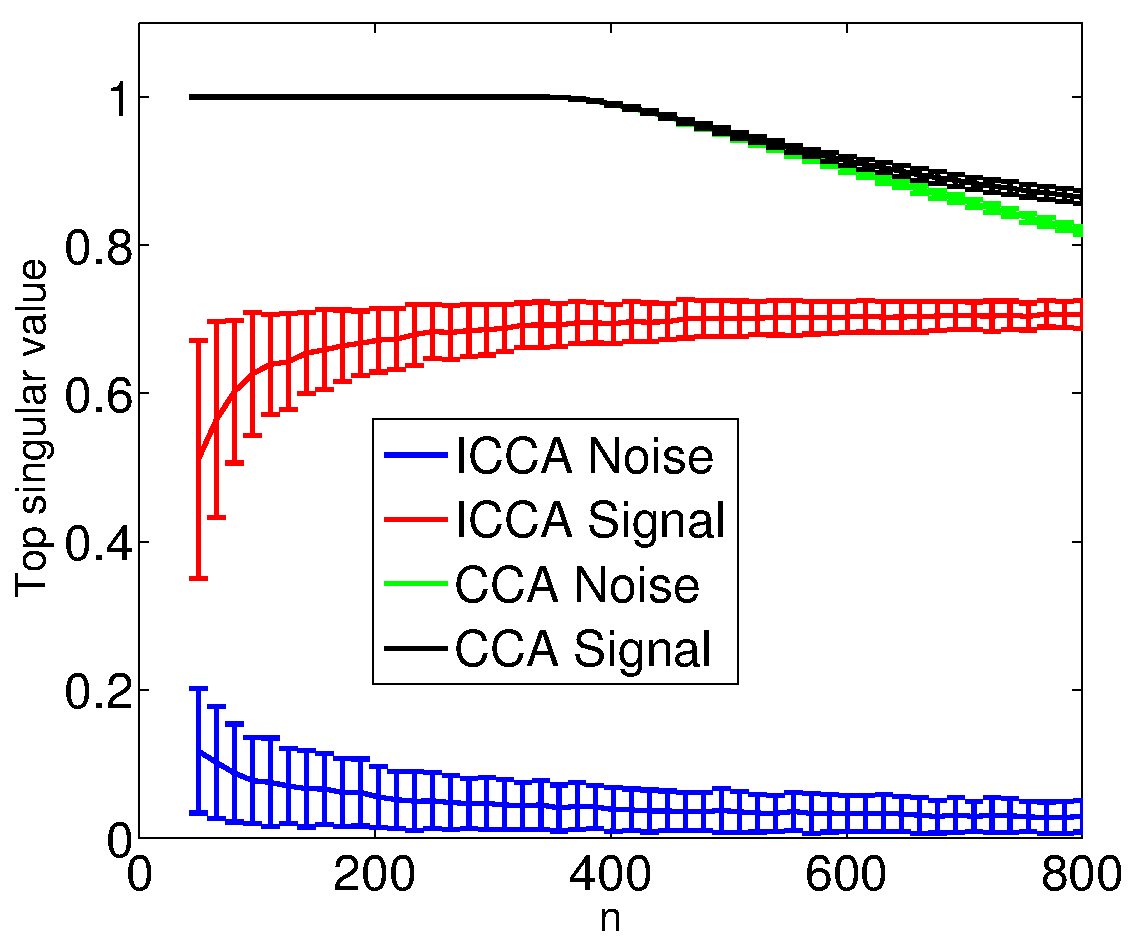
\includegraphics[width=\figwidth]{figures/icca_errorbars_high.pdf}
    \label{fig:icca_errorbars_high_snf}
  }
  \caption{Empirical distribution of the top singular value of $\widetilde{C}$ in
    (\ref{eq:icca_chat}) for both noise and signal data models in
    (\ref{eq:cca_data_model1}). Simulations were conducted using $d_1=200$, $d_2=150$,
    $\rho=0.9$, and $r_1=r_2=1$. The top singular value was computed for 500 trials. The
    mean top singular value is plotted with $\pm$ one standard deviation errorbars.}
  \label{fig:icca_errorbars}
\end{figure}

The results of the empirical distribution of the top singular value of $\widetilde{C}$ are
new. We immediately see many desirable characteristics of ICCA. First, the value of the
top singular value is no longer deterministically 1 when $n<d_1+d_2$. Second, as the
number of available training samples increases, $\tilde{\rho}^{\text{signal}}$ increases
for both values of $\sigma$.  This is desirable because it indicates that with more data,
the estimator is more confident that there is correlation between the dataset. Similarly,
with less data, the estimator is less confident that the datasets are correlated. As the
number of training samples increases, $\widetilde{\rho}^{\text{noise}}$ decreases to 0.
As the noisy datasets are uncorrelated ($\rho=0$), we would like the estimator to indicate
exactly this. The ICCA correlation estimate has this desirable property. Lastly, we note
that ICCA separates the distributions further and with less training data than CCA, even
under low SNR settings. Next, we use the KS statistic to explore when the empirical
distributions of $\widetilde{\rho}^{\text{noise}}$ and $\widetilde{\rho}^{\text{signal}}$
are statistically different. Results are shown in Figure \ref{fig:icca_ks_heatmap} with
the CCA KS heatmap presented again for ease of comparison.

\begin{figure}
  \subfigure[CCA]{
    \centering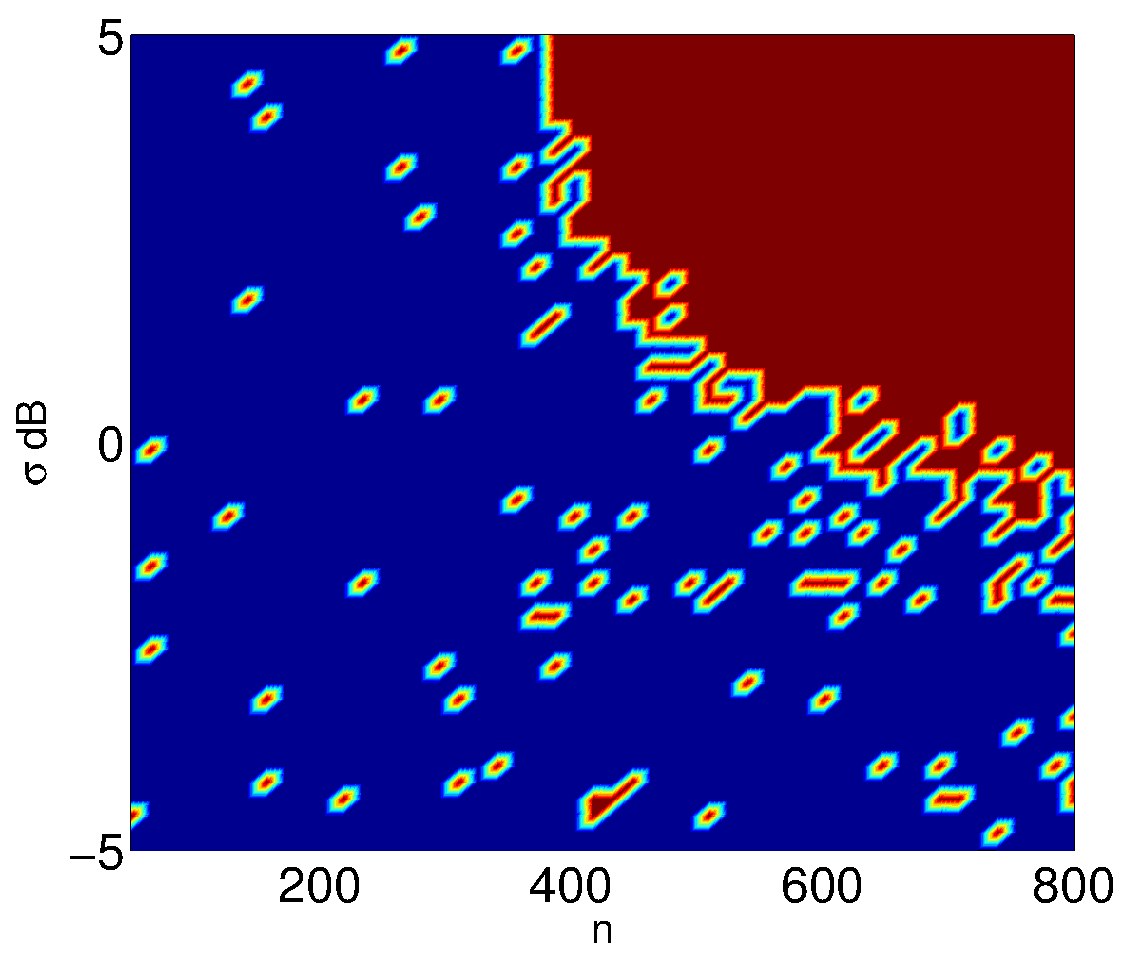
\includegraphics[width=\figwidth]{figures/cca_ks_heatmap.pdf}
  }
  \subfigure[ICCA]{
    \centering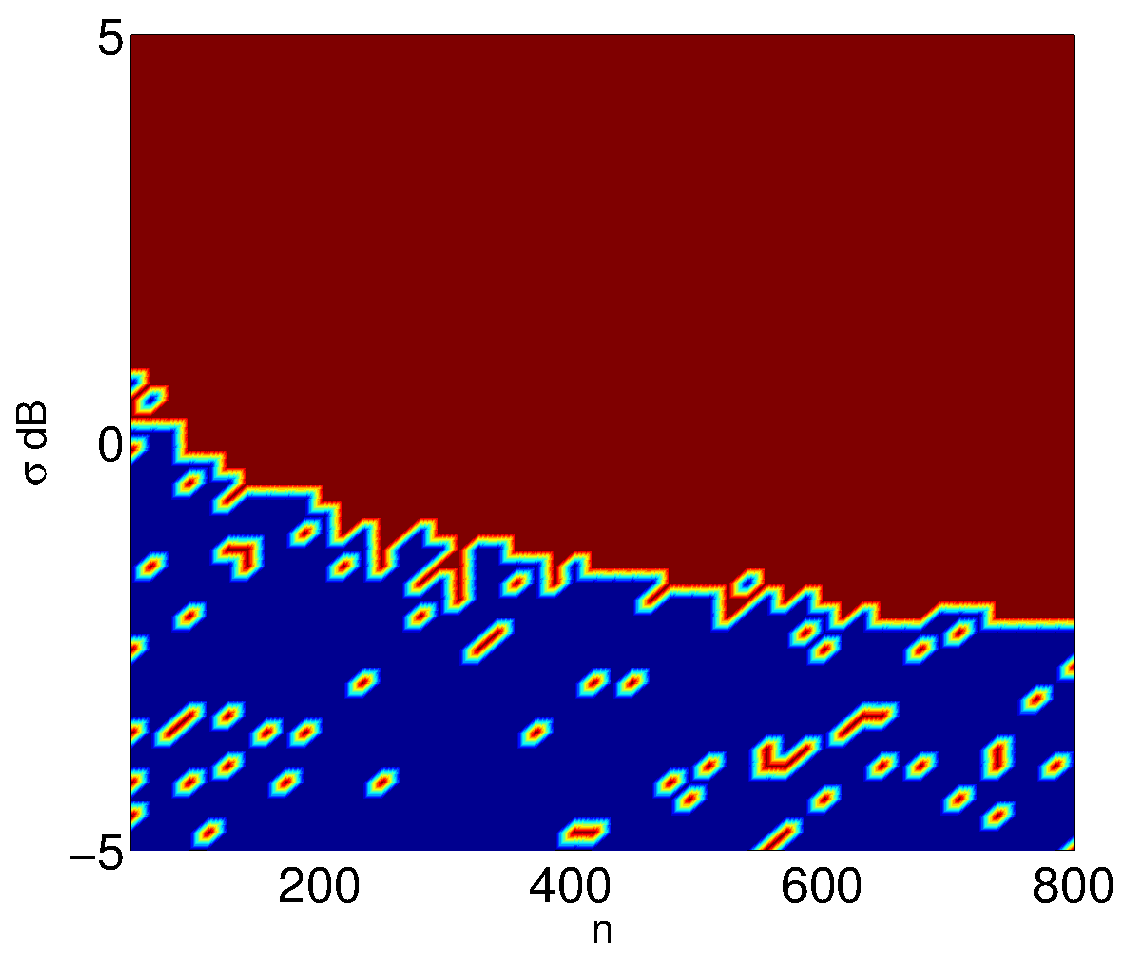
\includegraphics[width=\figwidth]{figures/icca_ks_heatmap.pdf}
  }
  \caption{Two-sided KS statistic between the empirical distributions of the leading
    singular value of $\widetilde{C}$ in (\ref{eq:icca_chat}) formed from training data
    generated from the noise and signal data models in
    (\ref{eq:cca_data_model1}). Simulations were conducted using $d_1=200$, $d_2=150$,
    $\rho=0.9$, $r_1=r_2=1$, 500 trials, and a significance level of $\alpha=0.95$ for the
    KS test. A value of 1 indicates the distributions are statistically different while a
    value of 0 indicates the distributions are statistically identical.}
  \label{fig:icca_ks_heatmap}
\end{figure}

This result confirms the result in \cite{nadakuditi2011fundamental}. Figure
\ref{fig:icca_ks_heatmap} shows that the empirical distributions of
$\widetilde{\rho}^{\text{noise}}$ and $\widetilde{\rho}^{\text{signal}}$ are statistically
different for a much larger number of combinations of $\sigma$ and $n$. In particular,
ICCA does not suffer from the performance breakdown at $n=d_1+d_2$ as CCA does. As one
would desire, given any number of training samples, the ICCA correlation estimates,
$\widetilde{\rho}^{\text{noise}}$ and $\widetilde{\rho}^{\text{signal}}$, are
statistically separable at a sufficiently large enough SNR. Intuitively, this SNR
threshold is larger for smaller values of $n$. For large $n$, ICCA can statistically
separate the distributions of $\widetilde{\rho}^{\text{noise}}$ and
$\widetilde{\rho}^{\text{signal}}$ at a lower SNR as compared to CCA. Finally, we explore
how separable these distributions are by examining the AUC for a na\"{\i}ve detector based
on the empirical correlation estimate returned by ICCA. These results are shown in Figure
\ref{fig:icca_auc_heatmap}. We present the AUC results from CCA again for ease of
comparison.

\begin{figure}
  \subfigure[CCA]{
    \centering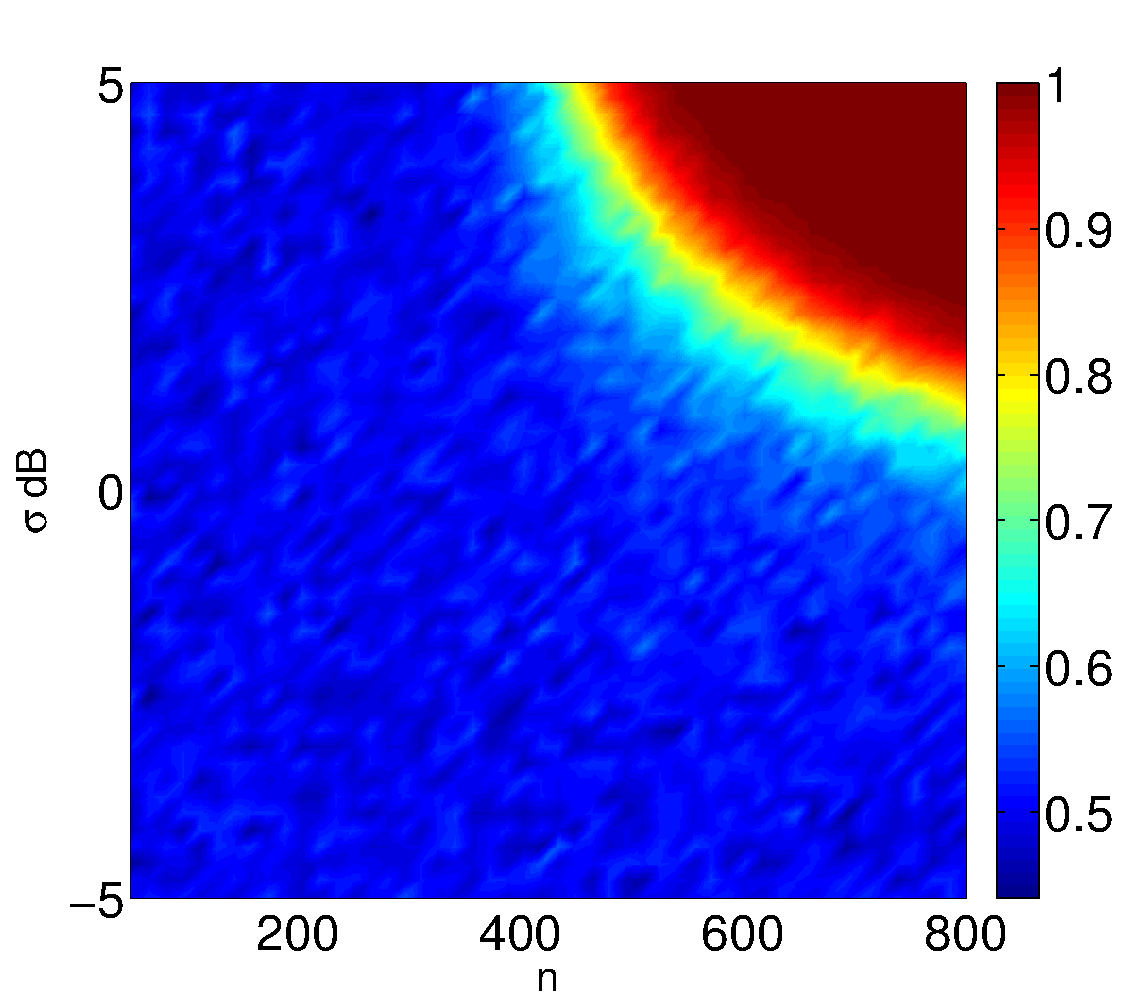
\includegraphics[width=\figwidth]{figures/cca_auc_heatmap.pdf}
  }
  \subfigure[ICCA]{
    \centering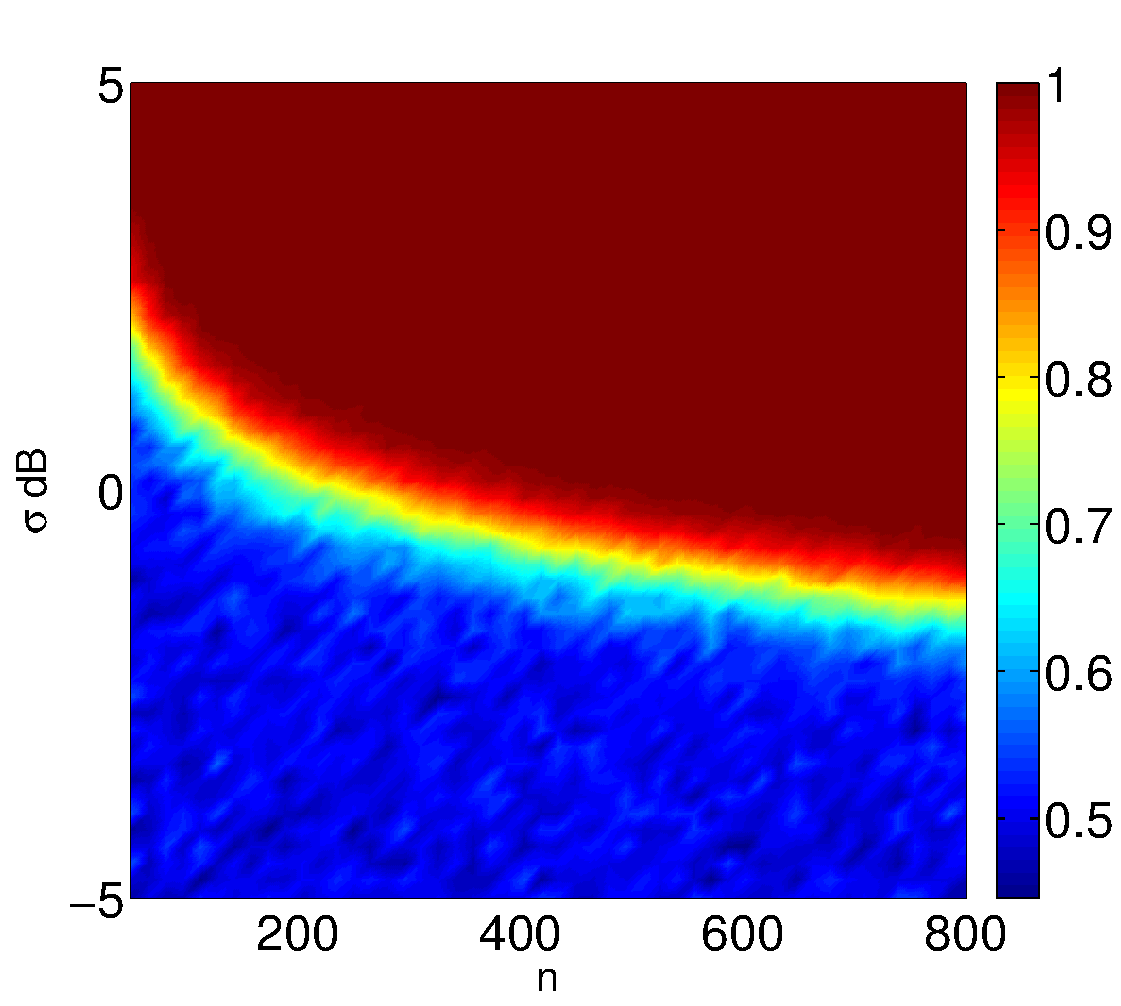
\includegraphics[width=\figwidth]{figures/icca_auc_heatmap.pdf}
  }
  \caption{AUC for a detector based on the top singular value of $\widetilde{C}$ in
    (\ref{eq:icca_chat}) to detect the noise and signal data models in
    (\ref{eq:cca_data_model1}). Simulations were conducted using $d_1=200$, $d_2=150$,
    $\rho=0.9$, 500 trials, and $r_1=r_2=1$.}
  \label{fig:icca_auc_heatmap}
\end{figure}

This is a new result. Similar to the KS statistic results in Figure
\ref{fig:icca_ks_heatmap}, the AUC results in Figure \ref{fig:icca_auc_heatmap} show that
ICCA outperforms CCA for a large number of combinations of $\sigma$ and $n$, most
importantly the sample starved regime. Again, for a fixed $n$, we observe a critical value
of $\sigma$, predicted by Proposition \ref{prop:raj}, above which signal detection is
possible. In the sample rich regime, ICCA can achieve perfect detection (AUC=1) for much
smaller values of SNR, which is highly desirable.

Clearly, the idea of trimming the training data SVDs to only include informative
components used in ICCA is beneficial. ICCA avoids the performance breakdown at
$n<d_1+d_2$ that is present in CCA. Furthermore, ICCA better separates the noise only and
signal distributions of the estimated correlation coefficient. Even in the sample rich
regime when many training data samples are available, ICCA is able to reliably detect
signals at a much lower SNR than CCA. CCA is not used often in the sample starved regime
because of this fundamental performance breakdown. Instead, it is common to use
regularized CCA (RCCA) in such a regime. In Chapter \ref{sec:rcca}, we explore the
performance of RCCA and apply the insights of informative data components to create an
informative version of RCCA. In the next chapter, we investigate applying CCA and ICCA to
matched subspace detection.

\section{Introduction} Canonical correlation analysis (CCA) is a classical joint
multidimensional dimensionality reduction algorithm for inferring or learning latent
correlations present in two datasets \cite{hotelling1936relations}. CCA learns a linear
transformation for each dataset such that the transformed features have maximal
correlation. Often, canonical correlation analysis is the first step in algorithms that
aim to fuse the information in the datasets to improve inference in the context of tasks
involving the detection, estimation, classification, and prediction of correlated
signals. CCA has been used in in machine learning \cite{hardoon2004canonical,
  dhillon2011multi, zhai2015instance, hardoon2006correlation,chaudhuri2009multi}, medical
signal processing, \cite{ correa2010canonical,arbabshirani2010comparison,
  khalid2013improving, lin2013identifying, seoane2014canonical, zhang2013l1,
  nakanishi2014enhancing, spuler2014spatial, kuzilek2014comparison},
economics \cite{todros2012measure}, climatology \cite{wilks2014probabilistic,
  prera2014using, steward2014assimilating}, and classical signal processing like Wiener
filters \cite{scharf1998wiener} and array processing \cite{ge2009does}.

In practice, when the population covariance and cross-covariance matrices of the two
datasets are unknown, they must be estimated from data. Empirical CCA relies on plug-in
estimates for these quantities. When the number of samples is large relative to the
combined dimensionality of the two datasets, empirical CCA performs well in the sense that
the empirical canonical correlation coefficients can be used to reliably infer the
presence of correlated signals buried in noise. However, when the sample size is less than
the combined dimensionality of the datasets the nthe empirical canonical correlation
coefficients will deterministically equal one, \textit{irrespective of whether there is a
  correlated signal in the datasets} \cite{pezeshki2004empirical}. This observation
led Pezeshki, Scharf et al to correctly conclude that in this regime
\begin{quote}
    ... the empirical canonical correlations are defective and may not be used as  estimates of canonical correlations between random
    variables.
\end{quote}
He et al. \cite{ge2009does} used extensive simulations to make a similar observation about
the deficiencies of empirical CCA in the sample size limited regime.

Recently, Bao et al \cite{bao2014canonical} rigorously studied the limiting behavior of
the empirical canonical correlation coefficients for the setting where the population
covariance matrix is arbitrary but the cross-covariance matrix is low rank. Their work
establishes the fundamental asymptotic limits of empirical CCA based detection of
correlated signals in noise in the general setting where the dimensionality of the system
is of the same order as the number of samples used to form the empirical covariance and
cross-covariance matrices. A conclusion from this analysis is the existence of a phase
transition threshold, which separates the regime where the low-rank signals are correlated
and can be detected using empirical CCA from a regime where they remain correlated but
cannot be detected using empirical CCA. More importantly, this phase transition threshold
depends explicitly on the degree of correlation between the signals. Particularly, as the
correlation decreases, the minimum (eigen) signal-to-noise ratio (SNR) above which
reliable detection is possible increases. Moreover, when there are not enough samples
relative to the combined dimensionality of the system, which includes the regime studied
by Pezeshki et al \cite{pezeshki2004empirical}, then the empirical correlation
coefficients will tend to one regardless of whether there is a correlated signal or not,
thereby crippling the inferential utility of empirical CCA based detection for the kinds
of high-dimensional ``large-$p$-relatively-small-$n$'' type problems that arise in modern
signal processing and machine learning
\cite{johnstone2008multivariate,fujikoshi2009high,wainwright2009sharp,yang2015computational,janson2015eigenprism}.

These results might convey to a practitioner that it is not theoretically possible to
detect the presence of correlated signals in two datasets for modern and emerging high
dimensional inferential problems. It is against this backdrop that we revisit this problem
from first principles. We consider the setting where the individual matrix-valued datasets
can be modeled as low-rank-correlated-signals-plus-noise type matrices; this model is
motivated by the ubiquity and success of low-rank models in practice
\cite{eckart1936approximation,candes2011robust,belkin2003laplacian,bach2003kernel,candes2011tight}. We
utilize the results of Bao et al \cite{bao2014canonical} and Pezeshki et al
\cite{pezeshki2004empirical} to establish the fundamental limits of empirical CCA for this
model. We then reconsider the connection between the canonical correlation coefficients
and angles between subspaces, and propose a simple modification to empirical CCA, which
builds on the work in \cite{nadakuditi2011fundamental}, that we label Informative CCA
(ICCA). We show that empirical CCA infers the presence of latent correlations by
considering the singular values of a matrix formed using all of the right singular vectors
of the individual signal-plus-noise matrices. In the regime where empirical CCA fails, a
subset of the right singular vectors of the individual matrices are ``informative'', i.e.,
positively correlated with the latent signal singular vectors. This insight motivates our
development of ICCA which infers the presence of latent correlations by considering the
singular values of a matrix formed using only these ``informative'' principal right
singular vectors of the individual signal-plus-noise matrices. In the setting where the
noise matrix is i.i.d. Gaussian, we also provide a principled approach, that leverages
using results from random matrix theory \cite{nadakuditi2010fundamental}, for selecting
the number of informative components.

We then establish the fundamental limits of inference using ICCA and bring into sharp
focus phase transitions that separate a regime where ICCA reliably infers (in an
asymptotic sense that we make precise) the presence of a correlated signal from a regime
where the correlation is present but ICCA fails. By comparing the derived fundamental
limits of ICCA with the fundamental limits for empirical CCA derived by Bao et al
\cite{bao2014canonical}, we are able to show that ICCA provably succeeds in reliably
detecting correlations in the sample deficient regime where empirical CCA provably
fails. Throughout this paper, when we say an algorithm ``provably succeeds'' we will mean
that the difference between the test statistic for the pure noise setting versus
correlated signal setting is almost surely positive. When we say that that the algorithm
``provably fails'' we mean that this difference is almost surely zero. The analysis also
reveals that the detection performance of ICCA does not depend on the correlation
coefficient, a very nice benefit over empirical CCA whose performance does depend on the
correlation coefficient. We show that our algorithm extends readily to the widely
considered missing data setting
\cite{candes2006stable,candes2009exact,cai2010singular,candes2010matrix,candes2010power}
and our analysis reveals that the benefits of ICCA over empircal CCA hold for this setting
as well as for a class of generalized noise models such as those considered in
\cite{benaych2012singular}.

The ICCA algorithm itself is relatively straightforward and we suspect that many
practitioners have used it or are already using it because they have observed numerically
that it ``works'' when empirical CCA does not. The main contribution of this work is the
establishment of a principled, mathematically rigorous framework that justifies the use of
ICCA based detection of correlated signals and the development of rigorous performance
guarantees for when we expect ICCA to succeed and the sorts of performance improvements we
can expect relative to empirical CCA. To the best of our knowledge, this is novel; in a
subsequent paper we will provide performance guarantees for canonical vectors estimated
using ICCA. The analysis of ICCA uses results established in
\cite{benaych2012singular,benaych2011eigenvalues} and extends them to consider the new
test statistic proposed herein. To that end, Theorem \ref{th:v_ip}, which is a crucial
tool used to prove Theorem \ref{th:khat_lims}, might be of independent interest to readers
with theoretical leanings. In addition to our many main results, we present some
theoretical conjectures that we believe to be true but which we were not able to
prove. Proving these conjectures will require a precise characterization of the limiting
behavior of of the empirical canonical correlation coefficients and their fluctuations and
the fluctuation behavior of the ICCA test statistic. We provide empirical evidence to lend
credence to our conjectures and hope that this will provide theoretically inclined readers
with an impetus for bridging this gap.

This paper is organized as follows. We provide the linear
low-rank-correlated-signal-plus-noise data model in Section \ref{sec:chpt4:model}. We then
derive the solution of CCA in Section \ref{sec:chpt4:cca} and show how to estimate the
number of correlated components from its solution. In Section \ref{sec:chpt4:emp_cca}, we
derive the empirical version of CCA using sample covariance matrices, highlight the
connection to angles between subspaces, and exploit that connection to present our
proposed ICCA algorithm. We then provide statistical tests to estimate the number of
correlated components present in the datasets for both empirical CCA and ICCA. We
summarize our main theoretical results in Section \ref{sec:chpt4:cca_theory}, highlighting
fundamental detection limits for empirical CCA (based on the work of Bao et al
\cite{bao2014canonical}) and ICCA (based on results we derive in this paper). We extend
this analysis to the missing data and non-Gaussian noise settings.  We verify these
theoretical results both on simulated data and real-world datasets in Section
\ref{sec:chpt4:emp}. Finally, we provide concluding remarks in Section
\ref{sec:chpt4:concl}.


\section{Setup}\label{sec:chpt4:model}

We assume that we are given $n$ observations of each dataset, which we stack columnwise to
form two data matrices
\begin{subequations}\label{eq:chpt4:data}
\beq
 X = [x_1,\dots,x_n]
\eeq
\beq
 Y = [y_1,\dots,y_n].
\eeq
\end{subequations}
It is important to note that the number of observations of each dataset must be the same and
that the observations come in pairs. For $i=1,\dots,n$, let $\xii\in\complex^{p\times 1}$
and $\yii\in\complex^{q\times 1}$ be modeled as
\begin{subequations}\label{eq:chpt4:data_model}
\beq
\xii = \Ux\sx + \zx
\eeq
\beq
\yii = \Uy\sy + \zy,
\eeq
\end{subequations}
where $\Ux^H\Ux=I_{\kx}$, $\Uy^H\Uy=I_{\ky}$, $\zx\simiid\mathcal{CN}(0,I_p)$ and
$\zy\simiid\mathcal{CN}(0,I_q)$. Furthermore, assume that
\be\ba
&\sx\sim\mathcal{CN}(0,\Tx)\\
&\sy\sim\mathcal{CN}(0,\Ty),\\
\ea\ee
where
\begin{subequations}\label{eq:chpt4:thetas}
\beq
\Tx=\diag\left(\left(\tx_1\right)^2,\dots,\left(\tx_{\kx}\right)^2\right)
\eeq
\beq
\Ty=\diag\left(\left(\ty_{1}\right)^2,\dots,\left(\ty_{\ky}\right)^2\right).
\eeq
\end{subequations}
Assume that $\zx$ and $\zy$ are
mutually independent and independent from both $\sx$ and $\sy$. Finally, assume that
\be
\E{\sx \sy^H} \defeq \Kxy = \Tx^{1/2}\Pxy\Ty^{1/2},
\ee
where the entries of $\Pxy$ are $-1\leq |\rho_{kj}| \leq 1$ and represent the correlation
between $\sx^{(k)}$ and $\sy^{(j)}$. For reasons to be made clear later, define
\be
\Kxytil = \left(\Tx+I_{\kx}\right)^{-1/2}\Kxy\left(\Ty+I_{\ky}\right)^{-1/2}
\ee
and define the singular values of $\Kxytil$ as
$\kappa_1,\dots,\kappa_{\min(\kx,\ky)}$. Under this model, we define the following
covariance matrices
\begin{subequations}\label{eq:chpt4:true_scm}
\beq\label{eq:chpt4:rxx}
\E{\xii\xii^H} = \Ux\Tx\Ux^H + I_p \defeq \Rxx
\eeq
\beq\label{eq:chpt4:ryy}
\E{\yii\yii^H} = \Uy\Ty\Uy^H + I_q \defeq \Ryy
\eeq
\beq\label{eq:chpt4:rxy}
\E{\xii\yii^H} = \Ux\Kxy\Uy^H \defeq \Rxy.
\eeq
\end{subequations}
Note that we may write $\sx=\Tx^{1/2} v_{x,i}$ and $\sy=\Ty^{1/2} v_{y,i}$ where
$v_{x,i}\sim\mathcal{CN}(0,I_{k_x})$ and $v_{y,i}\sim\mathcal{CN}(0,I_{k_y})$ are
independent random vectors. Defining $\Zx = [z_{x,1},\dots,z_{x,n}]$, $\Zy =
[z_{y,1},\dots,z_{y,n}]$, $\Vx=[v_{x,1},\dots,v_{x,n}]$, and $\Vy=[v_{y,1},\dots,v_{y,n}]$, we may write our data
matrices in (\ref{eq:chpt4:data}) as the sum of a low-rank signal matrix and noise
matrix
\begin{subequations}\label{eq:chpt4:data_matrices}
\beq
 X = \Ux\Tx^{1/2}\Vx^H + \Zx
\eeq
\beq
 Y = \Uy\Ty^{1/2}\Vy^H + \Zy.
\eeq
\end{subequations}

\section{Canonical Correlation Analysis and its variants}\label{sec:chpt4:cca}

Canonical Correlation Analysis (CCA) is a dimensionality reduction algorithm that finds
linear transformations for $\xii$ and $\yii$ such that in the projected spaces, the
transformed variables
are maximally correlated. Specifically, CCA solves the following optimization problem
\beq\label{eq:chpt4:opt_cca}
\rhocca =\max_{\wx,\wy} \frac{\wx^H\Rxy\wy}{\sqrt{\wx^H\Rxx\wx}\sqrt{\wy^H\Ryy\wy}},
\eeq
where $\wx$ and $\wy$ are called canonical vectors and $\rhocca$ is called the canonical
correlation coefficient. Notice that we can scale $\wx$ and
$\wy$ and still achieve the same objective function. Therefore, we may constrain the
canonical variates to have unit norm, resulting in the optimization problem
\beq\label{eq:chpt4:cca}\ba
&\max_{\wx,\wy} &&\wx^H\Rxy\wy\\
&\text{subject to} && \wx^H\Rxx\wx = 1\\
&&& \wy^H\Ryy\wy=1.\\
\ea\eeq
Substituting the change of variables $\wxt=\Rxx^{1/2}\wx$ and
$\wyt=\Ryy^{1/2}\wy$ in (\ref{eq:chpt4:cca}) results in the following optimization problem
\beq\label{eq:chpt4:cca_svd}\ba
&\max_{\wxt,\wyt} &&\wxt^H\Rxx^{-1/2}\Rxy\Ryy^{-1/2}\wyt\\
&\text{subject to} && \wxt^H\wxt = 1\\
&&& \wyt^H\wyt=1.\\
\ea\eeq
Examining the optimization problem in (\ref{eq:chpt4:cca_svd}), we can immediately see that the
solution to CCA may be solved via the SVD of the matrix
\beq\label{eq:chpt4:c_cca}
\Ccca = \Rxx^{-1/2}\Rxy\Ryy^{-1/2}.
\eeq
Define $\Ccca=FKG^T$ as the SVD of $\Ccca$ where $F$ is an unitary
$p\times p$ matrix with columns $f_1,\dots,f_p$, $G$ is a unitary $q\times q$ matrix with
columns $g_1,\dots,g_q$, and
$K=\diag(k_1,\dots,k_{\min(p,q)})$ is a $p\times q$ matrix whose diagonal elements are the
singular values of $\Ccca$. Therefore, the solution to (\ref{eq:chpt4:cca_svd}) is
\be\ba
\wxt = f_1\\
\wyt = g_1\\
\rho_{\text{cca}} = k_1.\\
\ea\ee
We can obtain higher order canonical correlations and vectors by taking successive singular
value and vector pairs. From this solution, it is clear that the number of non-zero
canonical correlation coefficients is exactly equal to the rank of $\Ccca$. Recalling the
definitions in (\ref{eq:chpt4:true_scm}),
$\Rxx$ and $\Ryy$ are non-singular so we have that
\be\ba
&\text{\# canonical correlation}&&=\rank(\Ccca)\\
&\text{   coefficients}&& = \rank(\Rxx^{-1/2}\Rxy\Ryy^{-1/2})\\
&&& = \rank(\Rxy)\\
&&& = \rank(\Kxy)\\
&&&\defeq k.\\
\ea\ee
Therefore, when we know all parameters, $k$ is exactly the number of non-zero singular
values of $\Kxy$. We note that $k\leq\min(\kx,\ky)$. Our  objective is to infer the number of non-zero canonical correlation coefficients from data.

\section{Detection of correlated signals using empirical and informative CCA}\label{sec:chpt4:emp_cca}
In many applications, we do not know the covariance matrices $\Rxx$, $\Ryy$, and $\Rxy$
\textit{a priori} and hence the quantities in
(\ref{eq:chpt4:true_scm}) are unknown. Consequently, we cannot determine the number
of canonical correlation coefficients by examining the rank of $\Rxy$. Instead, given
the data matrices in (\ref{eq:chpt4:data}), we form estimates of our unknown covariance
matrices via
\be\ba
& \Rxxhat = \frac{1}{n}XX^H\\
& \Ryyhat = \frac{1}{n}YY^H\\
& \Rxyhat = \frac{1}{n}XY^H.\\
\ea\ee
Define the data SVDs of the matrices in (\ref{eq:chpt4:data}) as
\be\ba
& X = \Uxhat\Sigxhat\Vyhat^H\\
& Y = \Uyhat\Sigyhat\Vyhat^H\\
\ea\ee
and trimmed matrices
\begin{subequations}\label{eq:chpt4:cca_trimmed}
\beq
 \Uxtil = \Uxhat\left(:,1:\min(p,n)\right)
\eeq
\beq
 \Vxtil = \Vxhat\left(:,1:\min(p,n)\right)
\eeq
\beq
 \Uytil = \Uyhat\left(:,1:\min(q,n)\right)
\eeq
\beq
 \Vytil = \Vyhat\left(:,1:\min(q,n)\right).
\eeq
\end{subequations}
Substituting the SVDs of sample analogs of the matrices in (\ref{eq:chpt4:c_cca}), reveals the insight (\cite[Eq. (6)]{nadakuditi2011fundamental}) that the matrix $\Ccca$ can be estimated as
\beq\label{eq:chpt4:cccahat}
\Cccahat = \Uxtil\Vxtil^H\Vytil\Uytil^H.
\eeq
We denote the singular values of this matrix by $\rhohatcca^{(j)}$ for $j=1,\dots,\min(p,q)$; these are precisely the empirical CCA correlation coefficients. Empirical CCA can return up
to $\min(p,q)$ canonical correlations; however, we know from the data model in
(\ref{eq:chpt4:data_model}) that $X$ and $Y$ have $\kx$ and $\ky$ underlying signals,
respectively. As $\kx$ and $\ky$ are unknown, let $\kxhat$ and $\kyhat$ be estimates of
the number of underlying signals in each dataset. As a consequence of (\ref{eq:chpt4:opt_cca})
we define the
plug-in estimates of $\rhocca$, as the $\min(\kxhat,\kyhat)$ singular values of $\Cccahat$ as
\beq\label{eq:chpt4:rhohatcca}
\rhohatcca^{(1)},\dots,\rhohatcca^{(\min(\kxhat,\kyhat))}.
\eeq
For now, we assume that we are given $\kxhat$ and $\kyhat$, but we will return to the
problem of estimating these parameters from data. To estimate the canonical vectors, we
use the corresponding left and right singular vectors of $\Cccahat$, $f_i$ and $g_i$ to
form
\begin{subequations}\label{eq:chpt4:cca_vects}
\beq
 w_x^{(i)} = \Rxxhat^{-1/2}f_i
\eeq
\beq
 w_y^{(i)} = \Ryyhat^{-1/2}g_i.
\eeq
\end{subequations}

When the number of samples is less than the combined dimension of the datasets ($n<p+q$),
the largest singular value of $\Cccahat$ is deterministically one
\cite{pezeshki2004empirical}, regardless of whether an underlying correlation actually
exists between the datasets. This is a very unfortunate property of empirical CCA as many of the motivating
applications operate in this low-sample, high-dimensionality regime. A key observation in
\cite{nadakuditi2011fundamental} shows that the singular values of $\Cccahat$ are exactly
the same as the singular values of $\Vxtil^H\Vytil$. This is a $\min(p,n)\times\min(q,n)$
matrix that uses all right singular vectors of each dataset corresponding to a non-zero
singular value. However, under the low-rank signal-plus-noise model,
\cite{nadakuditi2011fundamental} shows that only a few of the right singular vectors
actually contain \textit{informative} signal. Therefore, by trimming $\Vxtil$ and $\Vytil$
to have only $\kxhat$ and $\kyhat$ columns, we can avoid the performance loss of empirical
CCA in the sample deficient regime. Define the trimmed data SVDs
\begin{subequations}\label{eq:chpt4:trimmed_svds}
\beq
 \Uxcir = \Uxhat\left(:,1:\kxhat\right)
\eeq
\beq
 \Vxcir = \Vxhat\left(:,1:\kxhat\right)
\eeq
\beq
 \Uycir = \Uyhat\left(:,1:\kyhat\right)
\eeq
\beq
 \Vycir = \Vyhat\left(:,1:\kyhat\right).
\eeq
\end{subequations}
Given these definitions, we define the informative CCA (ICCA) matrix
\beq\label{eq:chpt4:ciccahat}
\Ciccahat = \Uxcir\Vxcir^H\Vycir\Uycir^H.
\eeq
Similar to empirical CCA, define the top $\min(\kxhat,\kyhat)$ singular values of $\Ciccahat$ as
\beq\label{eq:chpt4:rhohaticca}
\rhohaticca^{(1)},\dots,\rhohaticca^{(\min(\kxhat,\kyhat))}.
\eeq
To estimate the ICCA canonical vectors, we
use the corresponding left and right singular vectors of $\Ciccahat$, $f_i$ and $g_i$, to
form
\begin{subequations}\label{eq:chpt4:icca_vects}
\beq
 w_x^{(i)} = \Rxxhat^{-1/2}f_i
\eeq
\beq
 w_y^{(i)} = \Ryyhat^{-1/2}g_i.
\eeq
\end{subequations}
For completeness, we will address the problem of estimating the canonical vectors in a
subsequent paper.

\subsection{New Statistical Tests for Correlation Detection}\label{sec:chpt4:new_test}
 Given the canonical correlation estimates from CCA and ICCA, we can
estimate the number of canonical correlations using the test statistics
\begin{subequations}\label{eq:chpt4:khats}
\beq
 \khatcca = \sum_{i=1}^{\min(p,q)} \indicator_{\left\{\left(\rhohatcca^{(i)}\right)^2
     >\taucca\right\}}
\eeq
\beq
 \khaticca = \sum_{i=1}^{\min(\kxhat,\kyhat)}
 \indicator_{\left\{\left(\rhohaticca^{(i)}\right)^2 >\tauicca\right\}},
\eeq
\end{subequations}
where $\indicator_{\left\{\cdot\right\}}$ is the indicator function and
\begin{subequations}\label{eq:chpt4:taus}
\beq
 \taucca = F^{-1}_{\text{cca}}(1-\alpha)
\eeq
\beq
 \tauicca = F^{-1}_{\text{icca}}(1-\alpha).
\eeq
\end{subequations}
Here $F_{\text{cca}}$ and $F_{\text{icca}}$ are the distributions of the square of the largest singular
value of $\Cccahat$ and $\Ciccahat$ for the null setting where $\Vxtil$ and $\Vytil$ are the
$\min(n,p)$ and $\min(n,q)$ columns of two independent Haar (or isotropically random)
distributed $n\times n$ matrices. The exact distribution of the squared singular values of
$\Cccahat$ and $\Ciccahat$ in
the null model is given in \cite{constantine1976asymptotic}. The distributions of the
square of the largest singular value of $\Cccahat$ and $\Ciccahat$ in the null model may be
approximated to second-order by the Tracy-Widom law \cite{johnstone2008multivariate} as
\begin{subequations}\label{eq:chpt4:taus}
\beq
\taucca \approx \sigma_{p,q,n}\twrc^{-1}(1-\alpha) + \mu_{p,q,n},
\eeq
\beq
\tauicca \approx \sigma_{kxhat,\kyhat,n}\twrc^{-1}(1-\alpha) + \mu_{\kxhat,\kyhat,n},
\eeq
\end{subequations}
where $\sigma_{n,p,q}$ is a scaling parameter and $\mu_{n,p,q}$ is a centering
parameter and $\twrc$ is the appropriate Tracy-Widom law for either real or complex
data. See Tables III and IV of \cite{nadakuditi2010fundamental} for values of these
parameters as well as algorithms to determine $\kxhat$ and $\kyhat$. For a similar
high dimensional analysis, see \cite{fujikoshi2009high}.

\begin{comment}
We note that
$\sigma=o(n^{-1/3})$ and $\mu=o(n^{-1/2})$ so that as $n\to\infty$ (for fixed $p$, $q$,
$\kxhat$, and $\kyhat$), $\taucca$ and $\tauicca$ both tend towards zero.

\subsection{Classical Wilks Lambda Correlation Test}\label{sec:chpt4:wilks}
To test the significance of the empirical CCA canonical correlation estimates, classical
methods \cite{hardle2007applied,bartlett1954note} employ the Wilks likelihood ratio statistic,
\be
\Lambda\left(\rhohatcca^{(1)},\dots,\rhohatcca^{(\min(p,q))}\right) = -\left(n-\frac{p+q
    +3}{2}\right)\log\left(\prod_{i=1}^k\left(1-\rhohatcca^{(i)2}\right)\right),
\ee
which approximately follows a chi-square distribution
\be
\Lambda\left(\rhohatcca^{(1)},\dots,\rhohatcca^{(\min(p,q))}\right)\sim\chi_{pq}^2.
\ee
To determine significance of $\rhohatcca^{(1}$, we
compare the statistic against a threshold to achieve a desired false alarm rate via
\beq\label{eq:chpt4:wilks}
\Lambda\left(\rhohatcca^{(1)},\dots,\rhohatcca^{(\min(p,q))}\right) \siggtrless \eta,
\eeq
where $\eta = Q^{-1}_{\chi_{pq}^2}\left(1-\alpha\right)$, $\alpha$ is a desired
probability of false alarm and $Q$ is the inverse cumulative distribution function of the
chi squared distribution with $p\times q$ degrees of freedom.

From our derivation in Section \ref{sec:chpt4:new_test}, we observe that the classical
Wilk's Lambda test is suboptimal for testing the presence of a correlation in the low-rank
signal-plus-noise model for both empirical CCA and ICCA. The Tracy-Widom distribution is
the exact distribution of the singular values of $\Cccahat$ and $\Ciccahat$ in the
asymptotic setting. Therefore, using the Wilk's test statistic to test the significance of
empirical CCA and ICCA singular values will either result in a decrease in detection
ability or increase if false alarm rate compared to the Tracy-Widom based tests.

\end{comment}
\section{Main Results}\label{sec:chpt4:cca_theory}

In this section we summarize the main theoretical results for empirical CCA and our new
ICCA algorithm. We derive parameter regimes where the estimates in (\ref{eq:chpt4:khats})
correctly infer the presence of correlated signals. We then extend these
results to include the cases when the data matrices have missing entries and when the
additive noise of the data model in (\ref{eq:chpt4:data_model}) is not Gaussian.

\subsection{Empirical CCA}\label{sec:empircal CCA limits}

\begin{prop}\label{prop:pezeshki}
Let $n,p,q\to\infty$ such that $p/n\to c_x$ and $q/n\to c_y$. Let $p+q\leq n$. Then the
largest singular value of $\Cccahat$ generated from data modeled in (\ref{eq:chpt4:data_model})
behaves as
\be
\rhohatcca^{(1)} = 1.
\ee
\end{prop}
\begin{proof}
See \cite{pezeshki2004empirical}, page 996.
\end{proof}

A consequence of Proposition \ref{prop:pezeshki} is that the sample canonical correlation
coefficients obtained using empirical CCA will equal one even when there is no correlation
signal present in the datasets. We now establish the limiting behavior of the sample
canonical correlation coefficients for the regime where they are not deterministically
equal to one. The following proposition is a result presented in \cite{bao2014canonical},
adopted using our notation.

\begin{prop}\label{prop:bao}
Let $n,p,q\to\infty$ such that $p/n\to c_x$ and $q/n\to c_y$. Assume that $p+q<n$. For
$i=1,\dots,\min(\kx,\ky)$, let $\rhohatcca^{(i)}$ be the $i$-th largest singular value
of $\Cccahat$ generated from data modeled in (\ref{eq:chpt4:data_model}). Then these singular
values behave as
{\footnotesize \beq\label{eq:chpt4:bao_cca}
\rhohatcca^{(i)} \convas \begin{cases} \sqrt{\kappa_i^2\left(1-c_x+\frac{c_x}{\kappa_i^2}\right)\left(1-c_y+\frac{c_y}{\kappa_i^2}\right)} & \textrm{ if }  \kappa_i^2 \geq r_c \\ \sqrt{d_r} & \textrm{ if } \kappa_i^2<r_c\end{cases}
\eeq}
where $\kappa_i$ are the singular values of $\Kxytil$ and
\beq\label{eq:chpt4:rc}
 r_c = \frac{c_xc_y+\sqrt{c_yc_y(1-c_x)(1-c_y)}}{(1-c_x)(1-c_y) +
  \sqrt{c_xc_y(1-c_x)(1-c_y)}}
\eeq
and
\beq\label{eq:chpt4:dr}
 d_r = c_x+c_y-2c_xc_y+2\sqrt{c_xc_y(1-c_x)(1-c_y)}.
\eeq
\end{prop}
\begin{proof}
  See \cite{bao2014canonical} for original proof our see our appendix for a proof
  providing the necessary mathematical manipulations to transform our data model to the
  one used in \cite{bao2014canonical}.
\end{proof}

Proposition \ref{prop:bao} brings into sharp focus the existence of a phase transition
that separates a regime where the sample canonical correlation coefficients can be used to
infer the presence of a correlated signal from a regime where it cannot. The phase
transition boundary depends on the correlation between the signals in the two datasets via
the $\kappa_i$ quantity. We will empirically verify this result by \cite{bao2014canonical}
and use it as a baseline for CCA to which we will compare our new estimate, ICCA.

The empirical CCA estimate of the number of correlated components is given by  (\ref{eq:chpt4:khats}). Since $\taucca \to \sqrt{d_r}$, we expect (\ref{eq:chpt4:khats}) to return the number of singular values greater than $\sqrt{d_r}$. Let
\beq\label{eq:chpt4:keff_cca}
k_{\text{eff}}^{\text{cca}} =  \sum_{i=1}^k\indicator_{\{\kappa_i^2 > r_c\}},
\eeq
denote the effective number of correlated components detectable by empirical CCA. Note
that, by definition, $k_{\text{eff}}^{\text{cca}} \leq k$. Proposition \ref{prop:bao}
shows that $k_{\text{eff}}^{\text{cca}}< k$ whenever some of the singular values are below
the phase transition threshold $r_c$. These observations lead to the following conjecture.

\begin{conj}\label{conj:khat_lims}
In the same setting as Proposition \ref{prop:bao}, we have that
\be\ba
& \Prob{\khatcca = k_{\text{eff}}^{\text{cca}}}\to 1 &&\text{ if } \kappa_k^2 >r_c \text{ and } n>p+q\\
\ea\ee
where $\kappa_i$ are the singular value of $\Kxytil$ and $r_c$ is given in
(\ref{eq:chpt4:rc}).
\end{conj}

\begin{comment}
\begin{proof}
  The conditions for the consistency of the CCA estimate follows from
  (\ref{eq:chpt4:bao_cca}). From this equation, we observe that the square of the smallest
  non-zero singular value of $\Kxytil$, $\kappa_k$, must be larger than the constant $r_c$
  for the canonical correlation estimate to be different statistically from noise.
\end{proof}
\end{comment}

\subsection{ICCA}\label{sec:chpt4:new_results}

We now provide analogous performance guarantees for ICCA and establish conditions that can
be used to identify broad regimes where ICCA reliably detects correlations but empirical
CCA, based on Proposition \ref{prop:bao}, does not.  Our analysis of ICCA relies on the
characterization of the entries of the matrix $\Vxcir^H\Vycir$. To that end, we provide the
following intermediate theorem.

\begin{Th}\label{th:v_ip}
Let $\Vxcir$ and $\Vycir$ be the trimmed right singular vectors defined in
(\ref{eq:chpt4:trimmed_svds}) of the data matrices generated from the data model in
(\ref{eq:chpt4:data_model}). In the asymptotic setting of Theorem \ref{th:w_ip} with
$p/n\to c_x$ and $q/n\to c_y$
\be
\left|\left[\Vxcir^H\Vycir\right]_{ij}\right|\convas \left|\kxy_{ij}\right|\alpha_{x,i}\alpha_{y,j},
\ee
where
\begin{subequations}\label{eq:chpt4:alphas}
\beq\label{eq:chpt4:alpha_x}
\alpha_{x,i} = \sqrt{1 - \frac{c_x + \tx_i}{\tx_i(\tx_i + c_x)}} \qquad \textrm{ if }
  \tx_i > c_x^{1/4},
\eeq
and
\beq\label{eq:chpt4:alpha_y}
\alpha_{y,j} = \sqrt{1 - \frac{c_y + \ty_j}{\ty_j(\ty_j + c_x)}} \qquad \textrm{ if }
  \ty_j > c_y^{1/4},
\eeq
\end{subequations}
and $ \kxy_{ij}$ are the entries of $\Kxy$.
\end{Th}
\begin{proof}
See Appendix for proof and Theorem \ref{th:w_ip}.
\end{proof}


\begin{comment}
A consequence of Theorem \ref{th:v_ip} is that when $\kxhat=\kx$ and $\kyhat=\ky$, the
smallest singular value of $\Vxcir^H\Vycir$ is greater than zero. Armed with this insight,
we are now in position to prove the consistency of the ICCA estimates of the number of
correlated signals in (\ref{eq:chpt4:khats}). This result directly allows us to compare
the performance of CCA and ICCA across various regimes and showcases the superiority of
ICCA.
\end{comment}

Theorem \ref{th:v_ip} allows us to establish the following result.

\begin{Th}\label{th:khat_lims}
Let $p,q,n\to\infty$ with $p/n\to c_x$ and $q/n\to c_y$. For
$i=1,\dots,\min(\kx,\ky)$, let $\rhohaticca^{(i)}$ be the $i$-th largest singular value
of $\Ciccahat$ defined as in (\ref{eq:chpt4:ciccahat}). Then, for data modeled as in
(\ref{eq:chpt4:data_model}), we have that if 
\be
\min_{i=1,\dots,\kx} \tx_i>c_x^{1/4} \text{ and }
\min_{i=1,\dots,\ky} \ty_i>c_y^{1/4},
\ee
then
\be
\rhohaticca^{(k)} > 0 \text{ almost surely},
\ee
where $k=\rank(\Kxy)$.
\end{Th}
\begin{proof}
See Appendix.
\end{proof}

Analogous to the empirical CCA setting, let
\beq\label{eq:chpt4:keff_icca}
k_{\text{eff}}^{\text{icca}} =  \sum_{i=1}^k\indicator_{\{\theta_i^{(x)}>c_x^{1/4}
  \text{and } \theta_i^{(y)} > c_y^{1/4}\}},
\eeq
denote the effective number of correlated components detectable by ICCA. Note that, by
definition, $k_{\text{eff}}^{\text{icca}} \leq k$. Comparing Theorem \ref{th:khat_lims}
and Proposition \ref{prop:bao}, it is easy to see that $k_{\text{eff}}^{\text{icca}} \geq
k_{\text{eff}}^{\text{cca}}$. The ICCA estimate of the number of correlated components is
given by (\ref{eq:chpt4:khats}). Since $\tauicca \to 0$, whenever $\kxhat$ and $\kyhat$
are consistent estimates of $\kx$ and $\ky$, we are led to the following conjecture.

\begin{conj}\label{conj:icca}
In the setting of Theorem \ref{th:khat_lims}, let $\khaticca$ denote the estimate of the number of correlated components as given by (\ref{eq:chpt4:khats}). Then we have that
\be\ba
& \Prob{\khaticca = k_{\text{eff}}^{\text{icca}}}\to 1,
\ea\ee
\end{conj}


\begin{comment}
Estimating the number of signals present in such signal-plus-noise models
has been extensively studied in
\cite{benaych2012singular,benaych2011eigenvalues,paul2007asymptotics}. These works show
that when the signal-to-noise ratio is larger than a threshold, we can reliably detect the
presence of signals in noisy measurements. Specifically, we refer the reader to Algorithm
2 of \cite{nadakuditi2010fundamental} for a practical implementation using the Tracy Widom
approximation of the largest eigenvalues of the sample correlation matrix to detect the
number of signals. These results show that the individual estimates of the number of
signals are consistent under the following conditions
\be\ba
&\kxhat\convas\kx && \text{ if } \min_{i=1,\dots,\kx}\tx_i>c_x^{1/4}\\
&\kyhat\convas\ky && \text{ if } \min_{i=1,\dots,\ky}\ty_i>c_y^{1/4}.\\
\ea\ee
This observation leads us to extend Theorem \ref{th:khat_lims} to Conjecture \ref{conj:icca}.
\end{comment}
%In this vain we have the following definition.
%\begin{Def}
%Let $\keff$ be the effective number of canonical correlation coefficients defined as
%\be
%\keff = \sum_{i=1}^{\min(\kx,\ky)} \left(\indicator_{\left\{\tx_i>c_x\right\}} \times
%  \indicator_{\left\{\ty_i>c_y\right\}}\right).
%\ee
%\end{Def}

\subsection{Extension to Missing Data}\label{sec:chpt4:missing}
We now consider the setting where our data matrices $X$ and $Y$ have missing entries. In
such as setting, our matrices are modeled similar to (\ref{eq:chpt4:data_matrices}) but
with additional masking matrices
\begin{subequations}\label{eq:chpt4:data_model_miss}
\beq
 X = \left(\Ux\Tx^{1/2}\Vx^H + \Zx\right)\odot M_x
\eeq
\beq
 Y = \left(\Uy\Ty^{1/2}\Vy^H + \Zy\right)\odot M_y
\eeq
\end{subequations}
where
\be\ba
& M^x_{ij} = \begin{cases} 1 & \text{ with probability } \gamma_x\\ 0 & \text{ with
    probability } 1-\gamma_x \end{cases},\\
& M^y_{ij} = \begin{cases} 1 & \text{ with probability } \gamma_y\\ 0 & \text{ with
    probability } 1-\gamma_y \end{cases}
\ea\ee
and $\odot$ denotes the Hadamard or element-wise product. Throughout this section we make
the following assumption on the entries of $\Ux,\Uy,\Vx,\Vy$. Recall the definitions for
$\Tx$ and $\Ty$ in (\ref{eq:chpt4:thetas}). This assumption ensures that
the columns of these matrices are not ``spiked''.

\begin{Assum}\label{assum:chpt4:coher}
In the missing data setting, assume that the columns of $\Ux$, $\Uy$, $\Vx$, and $\Vy$
satisfy a `low-coherence' condition in the following sense: we suppose that there exist
non-negative constants $\eta_{u,x}$, $C_{u,x}$, $\eta_{u,y}$, $C_{u,y}$, $\eta_{v,x}$,
$C_{v,x}$,$\eta_{v,y}$, $C_{v,y}$ independent of $p$, $q$ and $n$, such that for $i=1,\dots,\kx$ and
$\j=1,\dots,\ky$,
{\small\be\ba
&\max_i \|u_i^{(x)}\|_\infty \leq \eta_{u,x}\frac{\log^{C_{u,x}}p}{\sqrt{p}}, \,\,\,\,
\max_i \|u_j^{(y)}\|_\infty \leq \eta_{u,y}\frac{\log^{C_{u,y}}q}{\sqrt{q}}\\
&\max_i \|v_i^{(x)}\|_\infty \leq \eta_{v,x}\frac{\log^{C_{v,x}}n}{\sqrt{n}}, \,\,\,\,
\max_i \|v_j^{(y)}\|_\infty \leq \eta_{v,y}\frac{\log^{C_{v,y}}n}{\sqrt{n}}.\\
\ea\ee}
\end{Assum}

In the missing data setting, our optimization problem remains unchanged
  from (\ref{eq:chpt4:opt_cca}), whose solution is given via the eigenvalue decomposition
  of $\Cccahat$ in (\ref{eq:chpt4:cccahat}). The only difference comes from the fact that
  the sample covariance matrices are formed via the data matrices in
  (\ref{eq:chpt4:data_model_miss}), which contain missing elements. In the same manner of
Section \ref{sec:chpt4:new_results}, we wish to provide performance guarantees in the
presence of missing data. The theorem below characterizes this behavior. We proceed as in
\cite{nadakuditi2014optshrink} and extensively use the results derived there. The two
theorems are very similar except that in the case of missing data, we simply replace $\Tx$
with $\gamma_x\Tx$ and $\Ty$ with $\gamma_y\Ty$. Therefore, missing data has the effect of
decreasing the SNR of our problem.

\begin{Th}\label{th:missing_data}
Let $p,q,n\to\infty$ with $p/n\to c_x>0$ and $q/n\to c_y>0$ and assume the coherence
conditions given in Assumption \ref{assum:chpt4:coher}. Given data modeled in
(\ref{eq:chpt4:data_model_miss}), we have that if 
\be
\min_{i=1,\dots,\kxhat}
\tx_i>\frac{c_x^{1/4}}{\sqrt{\gamma_x}} \text{ and }
\min_{i=1,\dots,\kyhat} \ty_i>\frac{c_y^{1/4}}{\sqrt{\gamma_y}}
\ee
then
\be
\rhohaticca^{(k)} > 0 \text{ almost surely},
\ee
where $k=\rank(\Kxy)$.
\end{Th}
\begin{proof}
See Appendix.
\end{proof}

\begin{conj}\label{conj:cca_missing}
For the same setting as in Theorem \ref{th:missing_data}, we have that
\be\ba
& \Prob{\rhohatcca^{(k)} > \sqrt{d_r} }\to 1 &&\text{ if } \min_{i=1,\dots,k}\kapcir_i^2 >r_c \text{ and } n>p+q\\
\ea\ee
where $r_c$ and $d_r$ are given in (\ref{eq:chpt4:rc}) and (\ref{eq:chpt4:dr}),
respectively, and $\kapcir_i$ are the singular values of
\be
\left(\gamma_x\Tx+I_{\kx}\right)^{-1/2}\left(\gamma_x\Tx\right)^{1/2}\Pxy\left(\gamma_y\Ty\right)^{1/2}
\left(\gamma_y\Ty+I_{\ky}\right)^{-1/2}.
\ee
\end{conj}

Proving Conjectures \ref{conj:khat_lims}, \ref{conj:icca}, and \ref{conj:cca_missing} requires a finer understanding of fluctuations of the test statistic than we presently have.

\subsection{Generalized Noise Model}

Finally, we provide a performance guarantee for non-Gaussian noise matrix models in (\ref{eq:chpt4:data_model}).

\begin{Assum}\label{assum:chpt4:noise}
Let $Z_x^{(n)} = [z_{x,1},\dots,z_{x,n}]$ be the $p\times n$ matrix formed by stacking $n$
observations of our noise. Let $Z_x^{(n)}$ have singular values
$\sigma_1\left(Z_x^{(n)}\right)\geq\cdots\geq\sigma_p\left(Z_x^{(n)}\right)$. Let
$\mu_{Z_x^{(n)}}$ be the empirical singular value distribution defined by the probability
  measure
\be
\mu_{Z_x^{(n)}} = \frac{1}{p}\sum_{i=1}^p \delta_{\sigma_i\left(Z_x^{(i)}\right)}.
\ee
We assume that the probability measure $\mu_{Z_x^{(n)}}$ converges almost surely weakly as
$p,n\to\infty$ with $p/n\to c_x$ to a non-random compactly supported probability measure
$\mu_{Z_x}$ that is supported on $[a_x,b_x]$. We assume that $\sigma_1\convas b_x$.

Similarly, we assume that the empirical singular value distribution for the noise matrix
of $Y$ converges almost surely to the non-random compactly supported probability measures
$\mu_{Z_y}$ that is supported on $[a_y,b_y]$ and that $\sigma_1\convas b_y$.
\end{Assum}


\begin{Corr}
  As in Assumption \ref{assum:chpt4:noise}, let $\mu_{Z_x}$ and $\mu_{Z_y}$ be the
  non-random compactly supported probability measures modeling the singular values of the
  noise matrices $X$ and $Y$. Let $b_x$ and $b_y$ be the supremums of the supports,
  respectively. Let $p,q,n\to\infty$ with $p/n\to c_x$ and $q/n\to c_y$. Relax the
  constraint in (\ref{eq:chpt4:data_model}) that the noise is Gaussian but instead drawn
  from the probability measures above. The ICCA canonical correlation estimates behave as
  \be
  \Prob{\rhohaticca^{(k)} > 0 }\to 1
  \ee
  if
  \be \min_{i=1,\dots,\kx}\tx_i>\frac{1}{D_{\mu_X}(b_x^+)}
  \text{ and} \min_{i=1,\dots,\ky}\ty_i > \frac{1}{D_{\mu_Y}(b_y^+)}
  \ee
  where $D_{\mu_X}$ and $D_{\mu_Y}$, the D-transforms of $\mu_X$ and $\mu_Y$, are the
  functions, depending on $c_x$ and $c_y$, defined by
  \be\ba
  &D_{\mu_X}(z)\defeq &&\left[\int\frac{z}{z^2-t^2}d\mu_X(t)\right]\times\\ &&&\left[
    c_x\int\frac{z}{z^2-t^2}d\mu_X(t) + \frac{1-c_x}{z}\right] \text{ for } z>b_x\\
  &D_{\mu_Y}(z)\defeq &&\left[\int\frac{z}{z^2-t^2}d\mu_Y(t)\right]\times\\ &&&\left[
    c_y\int\frac{z}{z^2-t^2}d\mu_Y(t) + \frac{1-c_y}{z}\right] \text{ for } z>b_y.
  \ea\ee
  Define the notation
  \be
  D_\mu(b^+) \defeq \lim_{z\downarrow b}D_\mu(z).
  \ee
\end{Corr}
\begin{proof}
This result follows from the proof of Theorem \ref{th:khat_lims} using the analysis in
\cite{benaych2012singular}.
\end{proof}
This is the more general result to Theorem \ref{th:khat_lims} as it is applicable to
non-Gaussian noise. See \cite{nadakuditi2014optshrink} for a discussion on
computing D-transforms in practice.

\section{Empirical Results}\label{sec:chpt4:emp}

\subsection{Simulated Data}

We first showcase the accuracy of the detection boundary for both empirical CCA and ICCA
described in Proposition \ref{prop:bao} and Theorem \ref{th:khat_lims}. We consider a
rank-1 setting ($\kx=\ky=1$) and generate data from (\ref{eq:chpt4:data_model}) for fixed
$p=q=150$ over various number of samples $n$, signal-to-noise ratio (SNR)
$\theta=\tx_1=\ty_1$, and various $\rho=\Pxy$. In this setting, there is only one
correlated signal so $k=1$ and the detection boundary becomes a phase transition. We
then form matrices $X$ and $Y$ and compute $\rhohatcca^{(1)}$ and
$\rhohaticca^{(1)}$ from the SVD of of $\Cccahat$ and $\Ciccahat$, respectively. Using
these correlation estimates, we compute the estimated number of correlated components via
(\ref{eq:chpt4:khats}) for a significance level of $\alpha=0.01$. For a fixed set of
parameters ($n$, $\theta$, $\rho$) we repeat the above process for 10000 trials and
determine the percentage of trials where we detect $\khatcca=1$ and $\khaticca=1$. In all
simulations, we use Algorithm 2 of \cite{nadakuditi2010fundamental} to estimate $\kxhat$
and $\kyhat$ using a significance level of $\alpha=0.01$. Figure \ref{fig:chpt4:cca_pt}
plots the $\log_{10}$ of this percentage for empirical CCA and ICCA for two values of
$\rho$. On each plot, we overlay the empirical CCA detection boundary given by Proposition
\ref{prop:bao} using a solid white line and the ICCA detection boundary given by
Theorem \ref{th:khat_lims} using a dashed white line.

From this figure, we see that for smaller $\rho$, it is more difficult for empirical CCA
to detect the presence of the correlated signal. However, ICCA is very robust to the
underlying correlation; the ICCA detection boundary in Theorem \ref{th:khat_lims} does not
depend on the value of $\rho$. We also verify Proposition \ref{prop:pezeshki} showing that
when $n<300$, it is impossible to detect the presence of correlated signals using
empirical CCA because $\rhohatcca=1$ deterministically. With ICCA, we avoid this
undesirable property and can still detect the presence of a correlated signal for very
small $n$ and $\theta$. This figure also provides evidence for Conjectures
\ref{conj:khat_lims} and \ref{conj:icca}.

\begin{figure*}
  \begin{center}
    \subfigure[Empirical CCA $\rho=0.7$]{
      \label{fig:chpt4:cca_rho7}
      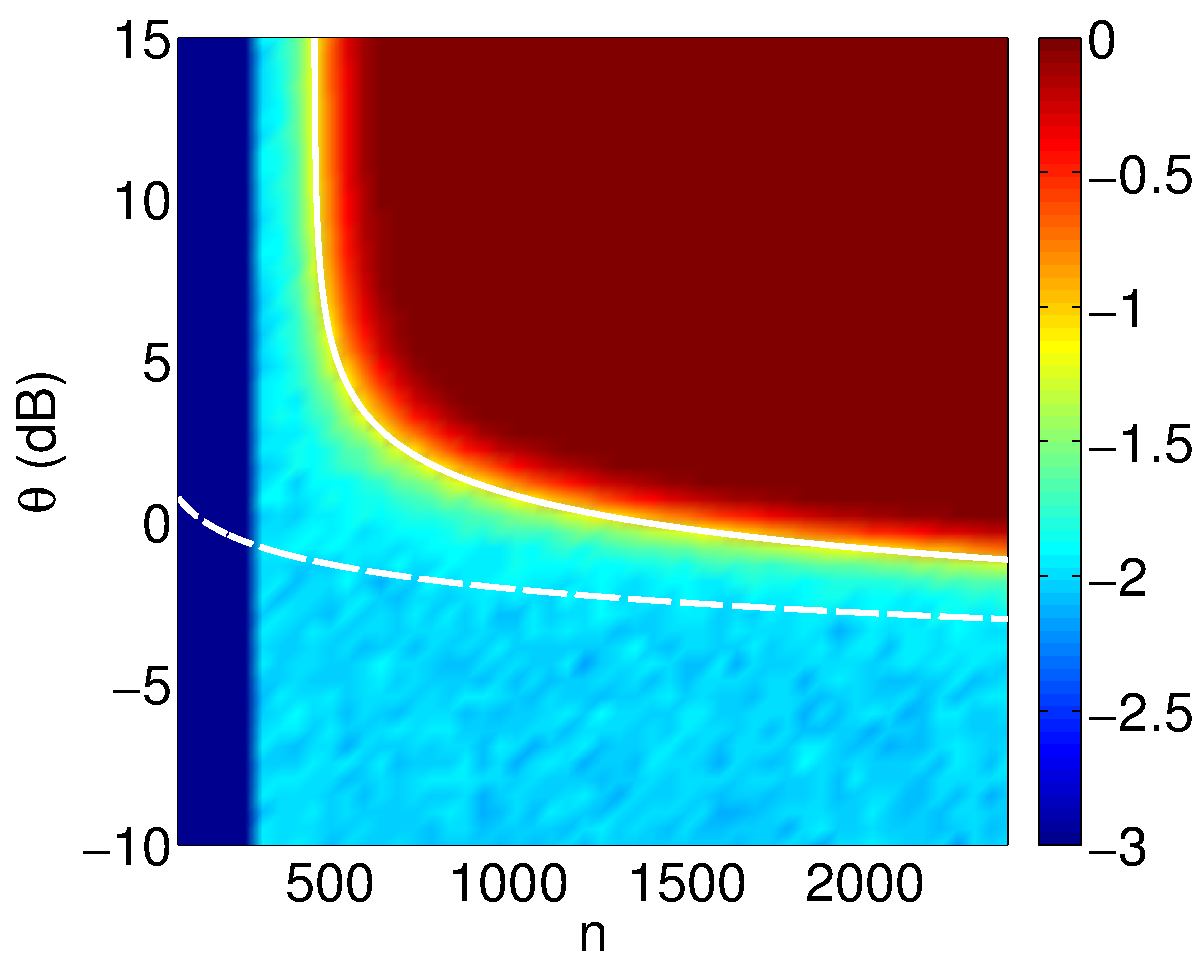
\includegraphics[width=0.4\textwidth]{figs/fig1a.pdf}
    }
    \subfigure[Empirical CCA $\rho=0.9$]{
      \label{fig:chpt4:cca_rho9}
      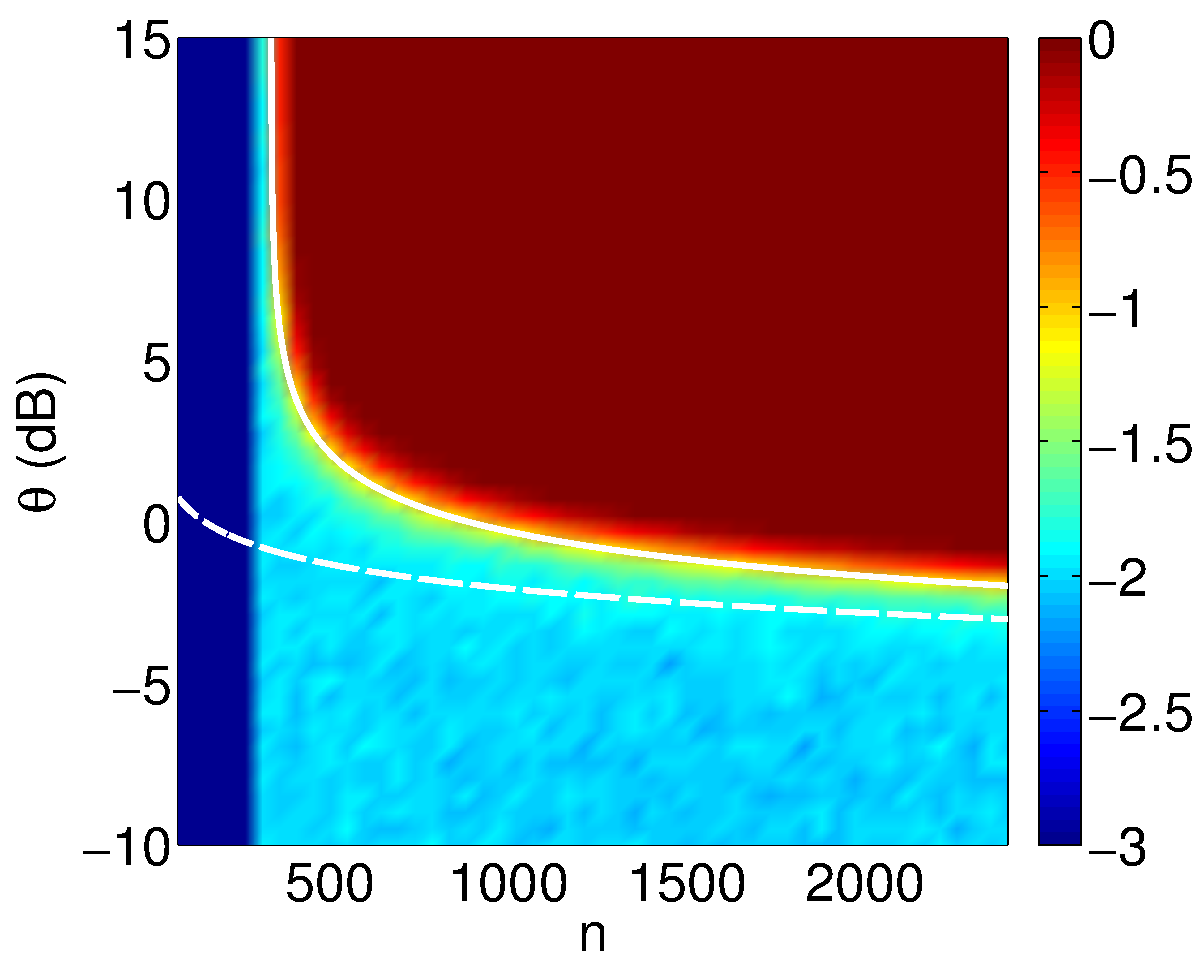
\includegraphics[width=0.4\textwidth]{figs/fig1b.pdf}
    }
    \subfigure[ICCA $\rho=0.7$]{
      \label{fig:chpt4:icca_rho7}
      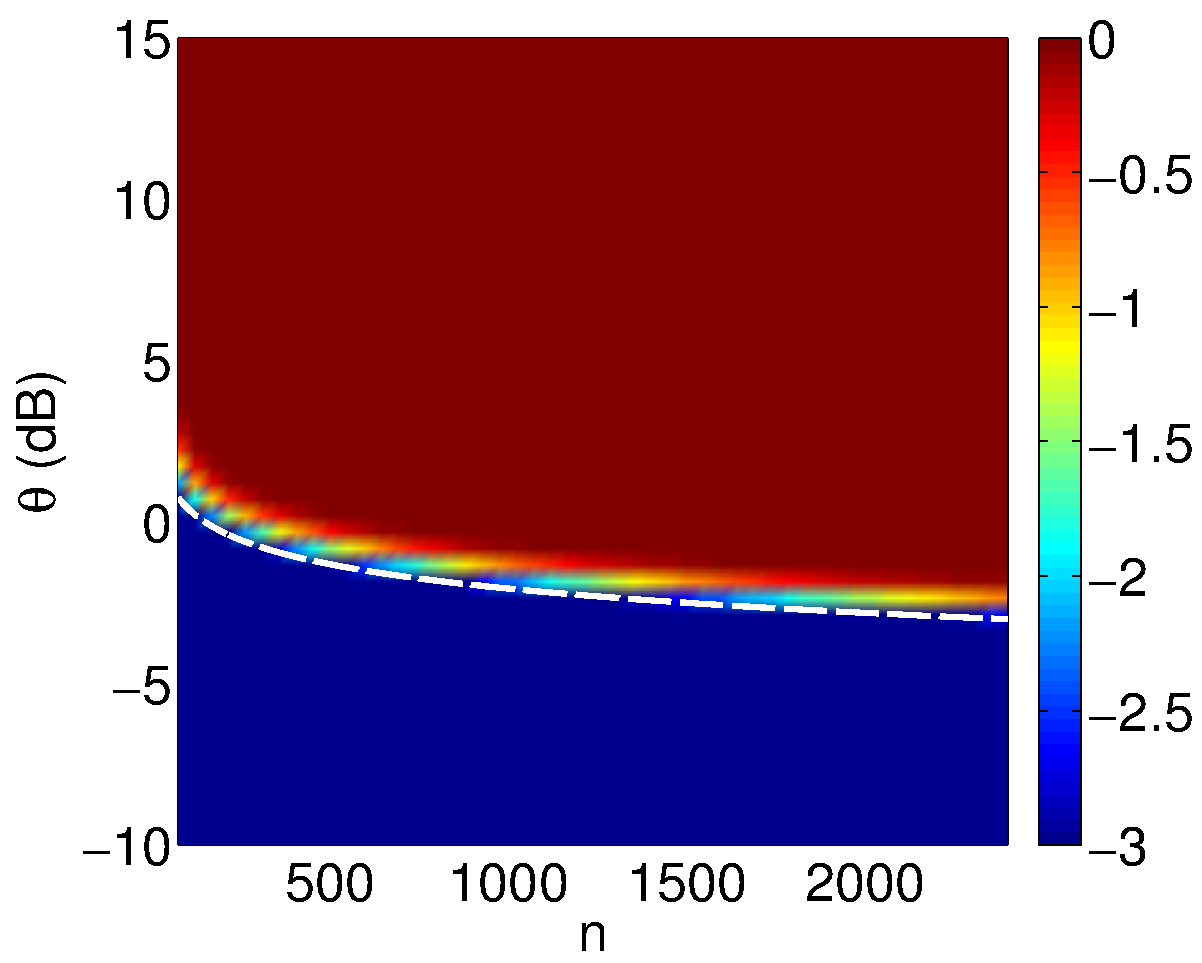
\includegraphics[width=0.4\textwidth]{figs/fig1c.pdf}
    }
    \subfigure[ICCA $\rho=0.9$]{
      \label{fig:chpt4:icca_rho9}
      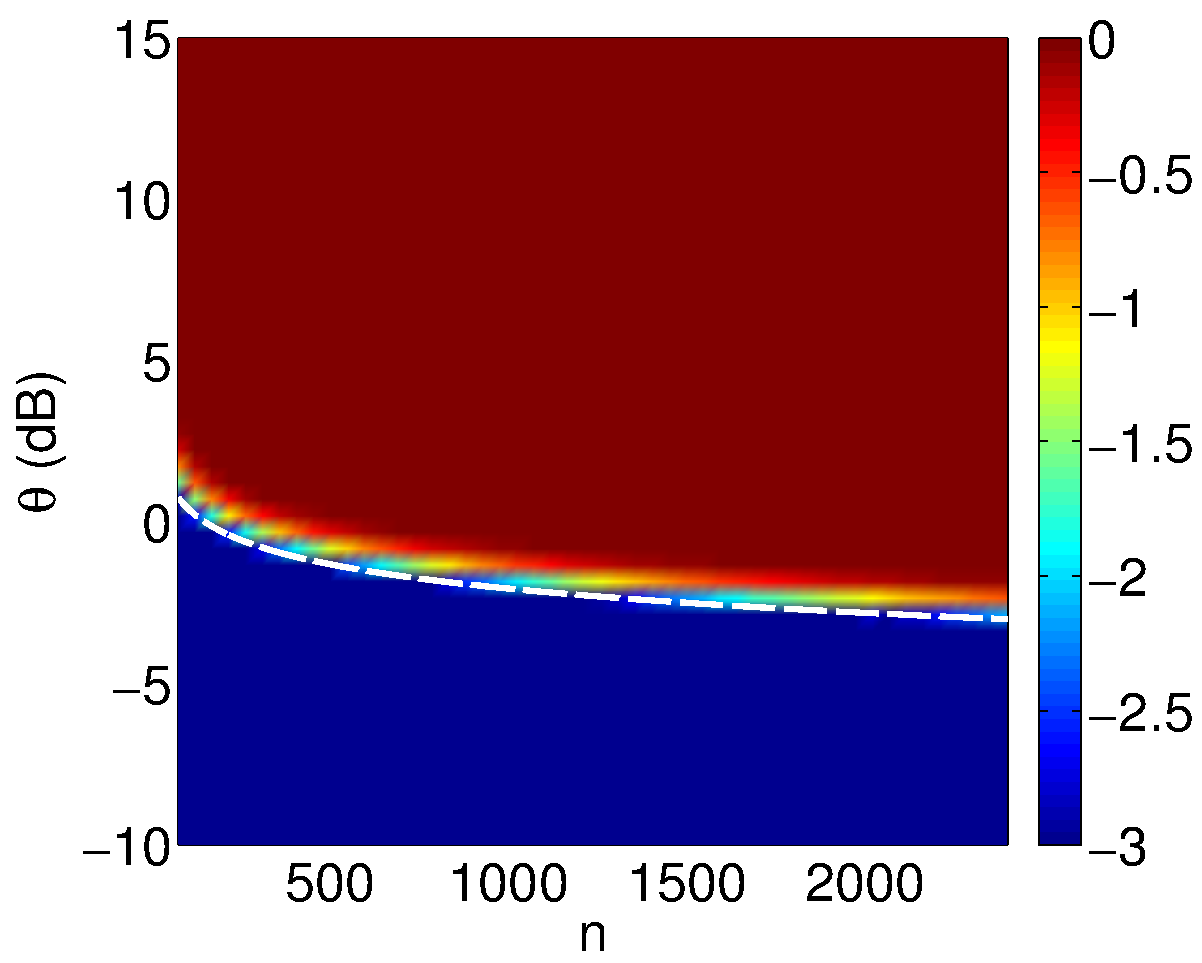
\includegraphics[width=0.4\textwidth]{figs/fig1d.pdf}
    }
    \caption{We generate data from (\ref{eq:chpt4:data_model}) for $p=q=150$, $\kx=\ky=1$,
      $k=1$, and various $\rho=\Pxy$ and sweep over $\theta = \tx_1=\ty_1$ and $n$. We
      compute $\kxhat$ and $\kyhat$ using Algorithm 2 of \cite{nadakuditi2010fundamental}
      for a significance value of $\alpha=0.01$. Using these estimates, we compute
      $\rhohatcca^{(1)}$ as the largest singular value of $\Cccahat$ as in
      (\ref{eq:chpt4:rhohatcca}) and $\rhohaticca^{(1)}$ as the largest singular value of
      $\Ciccahat$ as in (\ref{eq:chpt4:rhohaticca}). We then estimate the number of
      correlated signals $\khatcca$ and $\khaticca$ via (\ref{eq:chpt4:khats}) for a
      significance level of $\alpha=0.01$. We repeat this for 10000 trials and compute the
      percentage of trials where $\khatcca=1$ and $\khaticca=1$. We plot $\log_{10}$ of
      these percentages for multiples values of $\theta$ and $n$. We plot the theoretical
      phase transition of empirical CCA (given in Proposition \ref{prop:bao} that
      relies on \cite{bao2014canonical}) in a solid white line and the theoretical
      phase transition of ICCA (given in Theorem \ref{th:khat_lims}) in a dashed white
      line.}
    \label{fig:chpt4:cca_pt}
  \end{center}
\end{figure*}

Next, we explore the minimum $1/c$ for $c=c_x=c_y$ needed to reliably detect $k=1$
correlated signal in the experiment setting described for Figure
\ref{fig:chpt4:cca_pt}. As $c=p/n=q/n$, the minimum $1/c$ is equivalent to the minimum
number of samples needed for fixed dimensions. Using the theoretical phase transitions in
Proposition \ref{prop:bao} and Theorem \ref{th:khat_lims}, we have that this critical
value of $c$ is $c_{\text{crit}} = \theta^4$ for ICCA and $c_{\text{crit}} =
\min\left(\frac{r_c^{\text{crit}}}{1+r_c^{\text{crit}}}, 0.5\right)$ for empirical CCA,
where \be r_c^{\text{crit}} = \left(\frac{-\rho +
    \sqrt{\rho^2+4\theta^2\rho^2(1+\theta^2\rho^2)}}{2(1+\theta^2\rho^2)}\right)^2.  \ee
Figure \ref{fig:chpt4:contours} plots level sets of $c_{\text{crit}}$ for empirical CCA
and ICCA for various values of $\theta=\tx_1=\ty_1$ and $\rho=\Pxy$. Recall that if
$c>0.5$, empirical CCA fails entirely, so for comparison we only show contour lines for
$1/c=10$ and $1/c=3$.

From this figure, we once again observe that the performance of ICCA is independent of the
value of $\rho=\Pxy$, while the performance of empirical CCA is highly dependent on the
correlation. This figure allows us to showcase that ICCA is theoretically better than
empirical CCA in all parameter regimes as ICCA can achieve the same performance of
empirical CCA given fewer samples at a lower SNR.

\begin{figure}
  \begin{center}
    \subfigure[Empirical CCA]{
      \label{fig:chpt4:cca_contours}
      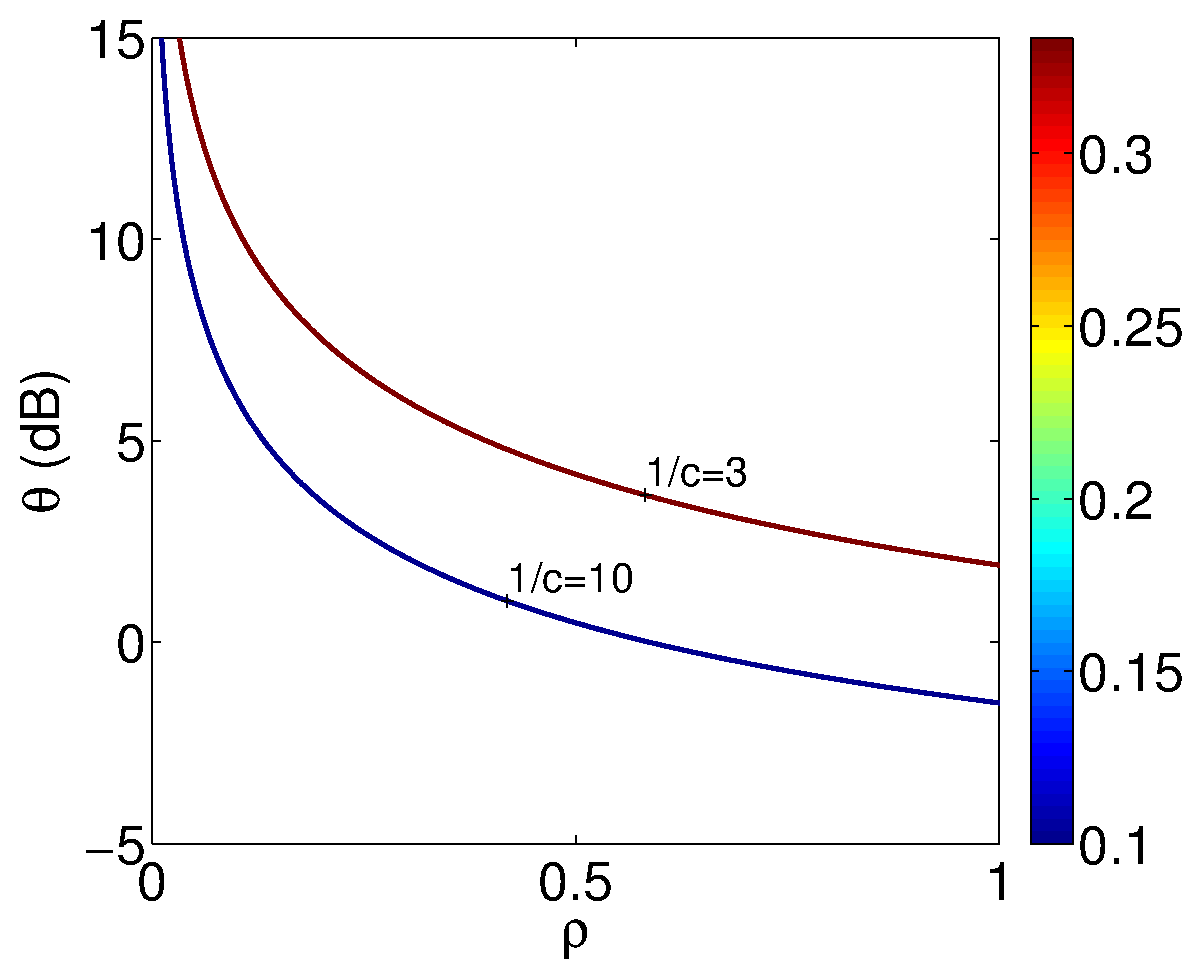
\includegraphics[width=0.4\textwidth]{figs/fig2a.pdf}
    }
    \subfigure[ICCA]{
      \label{fig:chpt4:icca_contours}
      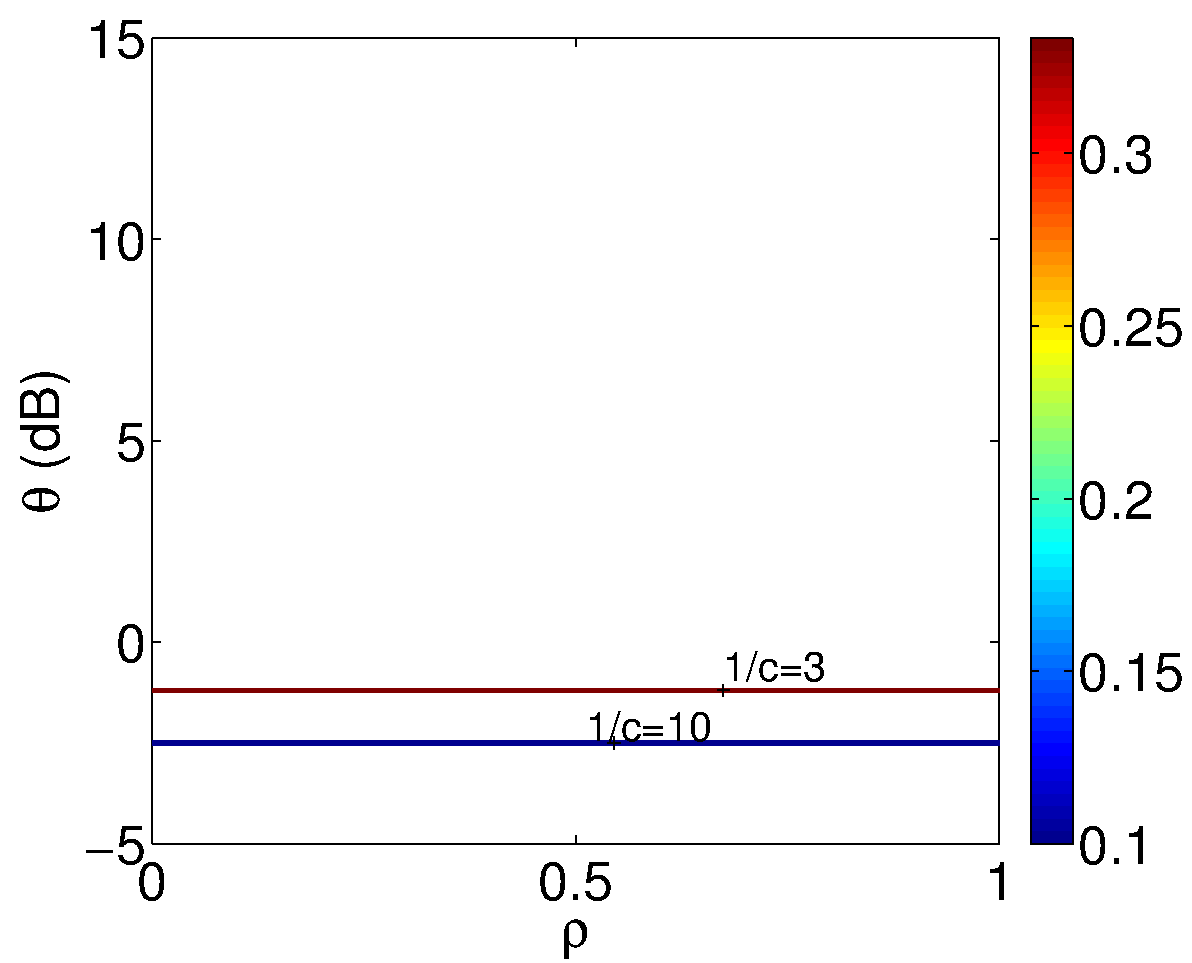
\includegraphics[width=0.4\textwidth]{figs/fig2b.pdf}
    }
    \caption{Contour lines for minimum $1/c$ necessary for reliable detection of $k=1$
      correlated component. The quantity $1/c = n/p$ is equivalent to the number of
      samples per dimension of data. For $c=c_x=c_y$, Figure \ref{fig:chpt4:cca_contours} plots the
      contours for empirical CCA using the limits given in Proposition \ref{prop:bao} and
      Figure \ref{fig:chpt4:icca_contours} plots the ICCA contours using the limits given
      in Theorem \ref{th:khat_lims}. We plot the contours for $1/c=10$ and
      $1/c=3$.  These plots clearly demonstrate that the ICCA limits are independent of
      $\rho=\Pxy$ while those for empirical CCA are highly dependent on $\rho=\Pxy$. For a fixed number of
      samples (fixed $c$), ICCA can reliably detect the presence of a correlated signal at
      lower SNR values than empirical CCA.}
    \label{fig:chpt4:contours}
  \end{center}
\end{figure}


\subsection{Simulated Missing Data}

Next, we demonstrate the accuracy of the performance limits for both empirical CCA and
ICCA in the setting of missing data described in Theorem \ref{th:missing_data} and
Conjecture \ref{conj:cca_missing}. Again, we consider a rank-1 setting ($\kx=\ky=1$) but
generate data from (\ref{eq:chpt4:data_model_miss}) for fixed $p=q=150$ over various
number of samples $n$, signal-to-noise ratio (SNR) $\theta=\tx_1=\ty_1$, various
$\rho=\Pxy$ (so that $k=1$), and also various percentages of missing data
$\gamma=\gamma_x=\gamma_y$. In all simulations, we use Algorithm 2 of
\cite{nadakuditi2010fundamental} to estimate $\kxhat$ and $\kyhat$ using a significance
level of $\alpha=0.01$. We stack the data into matrices $X$ and $Y$ and compute
$\rhohatcca^{(1)}$ and $\rhohaticca^{(1)}$ from the SVD of of $\Cccahat$ and $\Ciccahat$,
respectively. Using these correlation estimates, we compute the estimated number of
correlated components via (\ref{eq:chpt4:khats}) for a significance level of
$\alpha=0.01$. For a fixed set of parameters ($n$, $\theta$, $\rho$, $\gamma$) we repeat
the above process for 10000 trials and determine the percentage of trials where we detect
$\khatcca=1$ and $\khaticca=1$. Figure \ref{fig:chpt4:cca_missing_75} plots the
$\log_{10}$ of this percentage for empirical CCA and ICCA, respectively. We
overlay the ICCA performance boundary given by Theorem \ref{th:missing_data} in a dashed line
and the empirical CCA performance boundary given by Conjecture \ref{conj:cca_missing} in a
solid line.

From these figures, we observe that Theorem \ref{th:missing_data} and Conjecture
\ref{conj:cca_missing} accurately predict the phase transition for both empirical CCA and
ICCA in the presence of missing data for a wide array of parameters. Even in the presence
of missing data, ICCA can detect the presence of the correlated signal in the low-sample
regime ($n<p+q$) where empirical CCA deterministically fails.  In this missing data
setting, we once again observe that the value of $\rho$ affects the phase transition for
empirical CCA but not for ICCA; it is harder for CCA to detect signals with small
correlations.

\begin{figure*}
  \begin{center}
    \subfigure[Empirical CCA $\rho=0.7$]{
      \label{fig:chpt4:cca_rho3_75}
      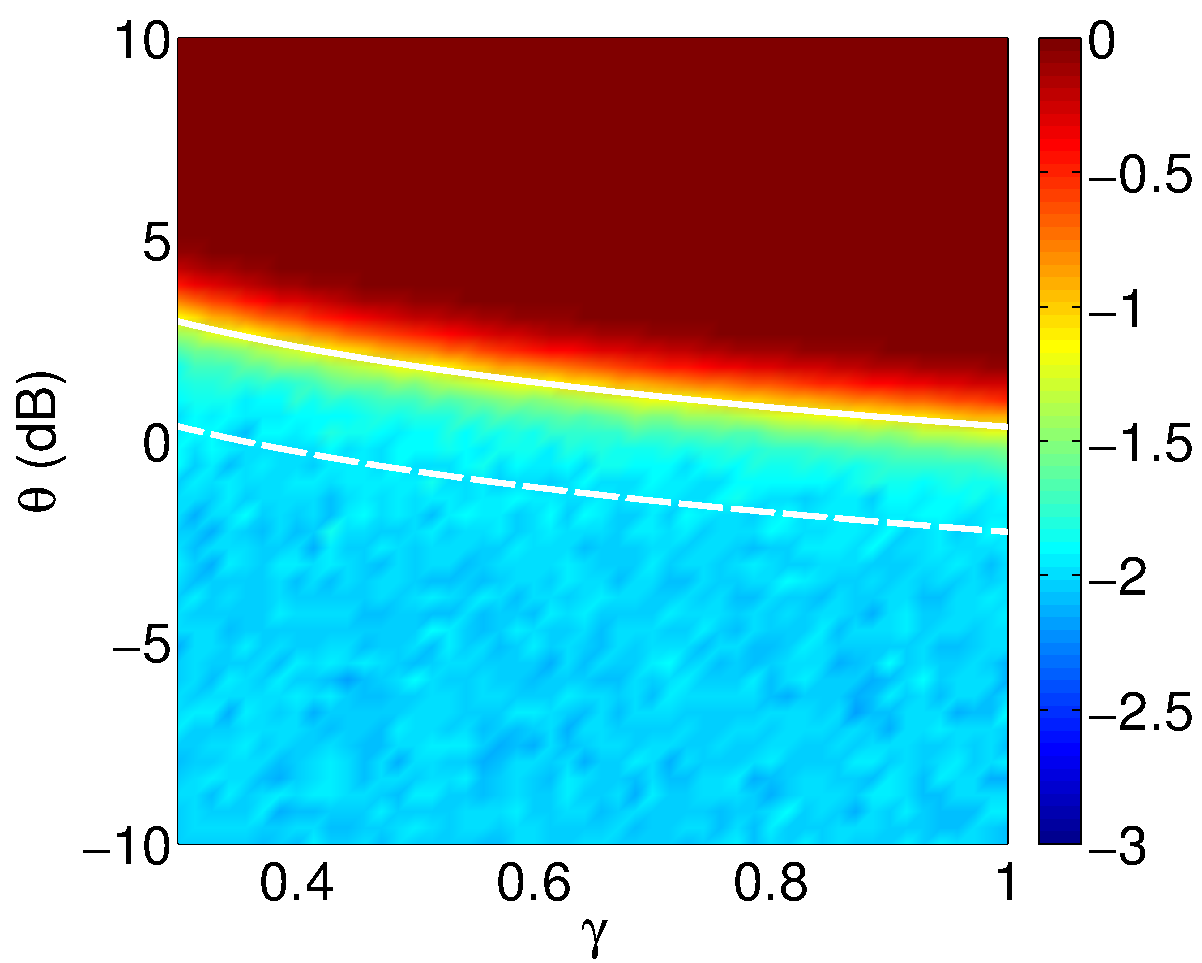
\includegraphics[width=0.4\textwidth]{figs/fig3a.pdf}
    }
    \subfigure[Empirical $\rho=0.9$]{
      \label{fig:chpt4:cca_rho5_75}
      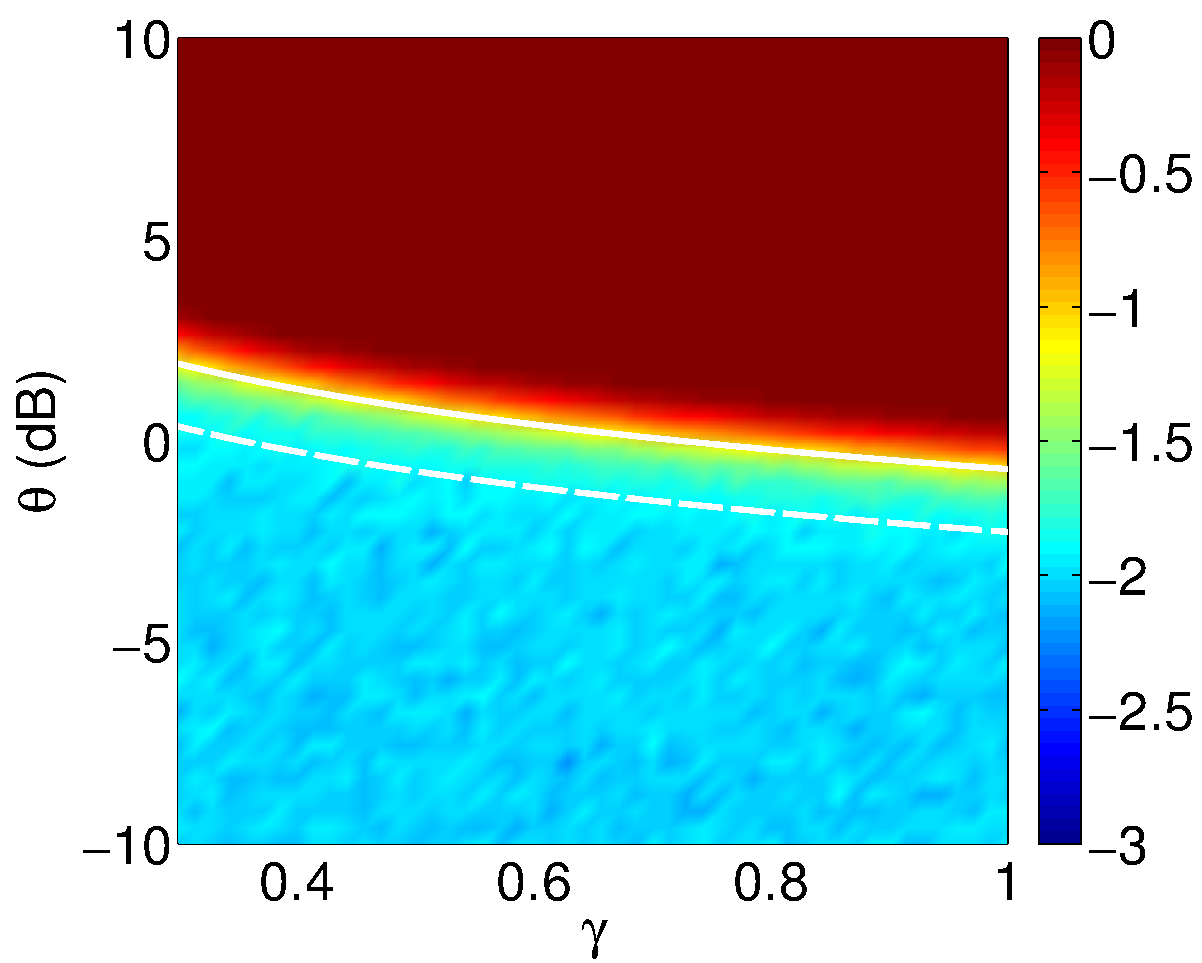
\includegraphics[width=0.4\textwidth]{figs/fig3b.pdf}
    }
    \subfigure[ICCA $\rho=0.7$]{
      \label{fig:chpt4:cca_rho7_75}
      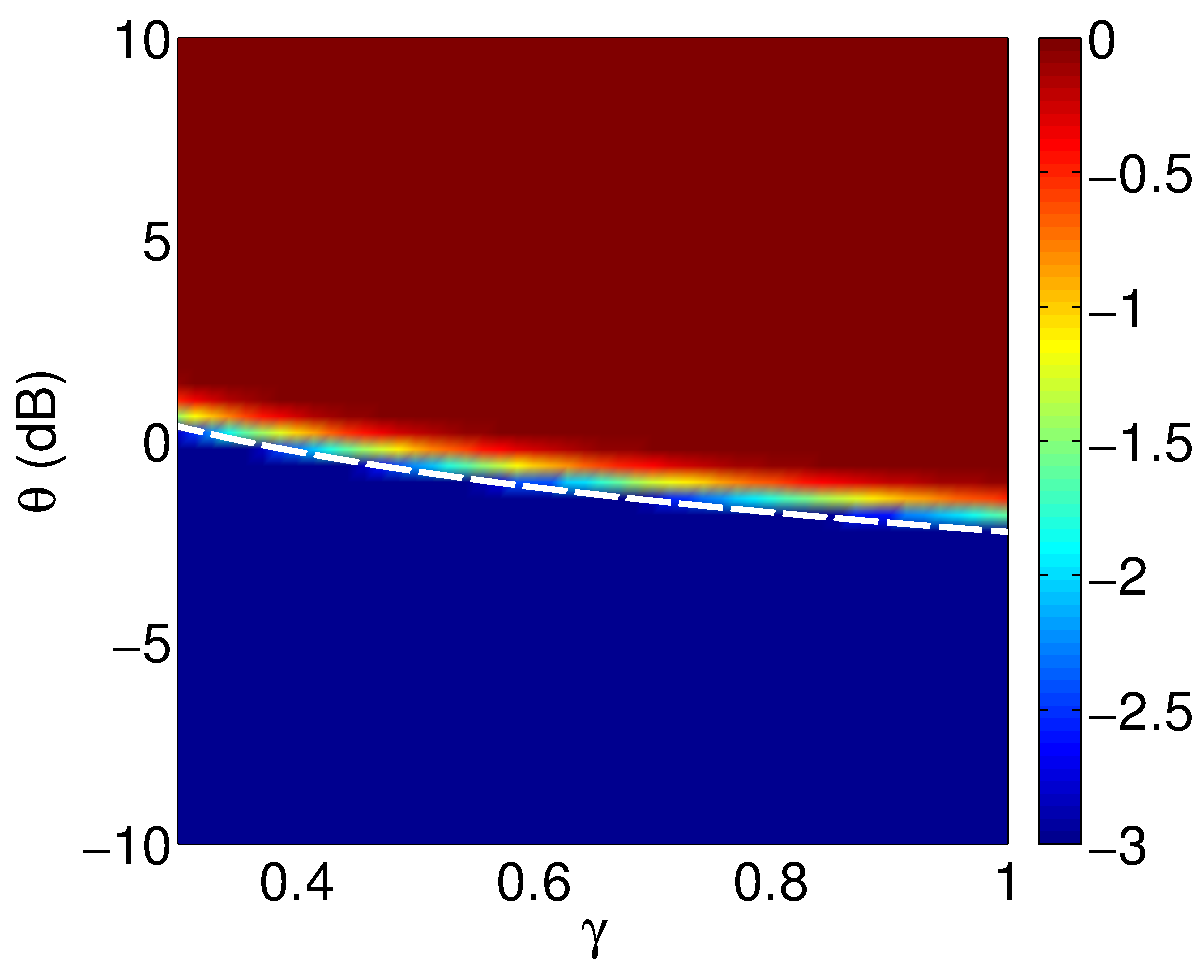
\includegraphics[width=0.4\textwidth]{figs/fig3c.pdf}
    }
    \subfigure[ICCA $\rho=0.9$]{
      \label{fig:chpt4:cca_rho9_75}
      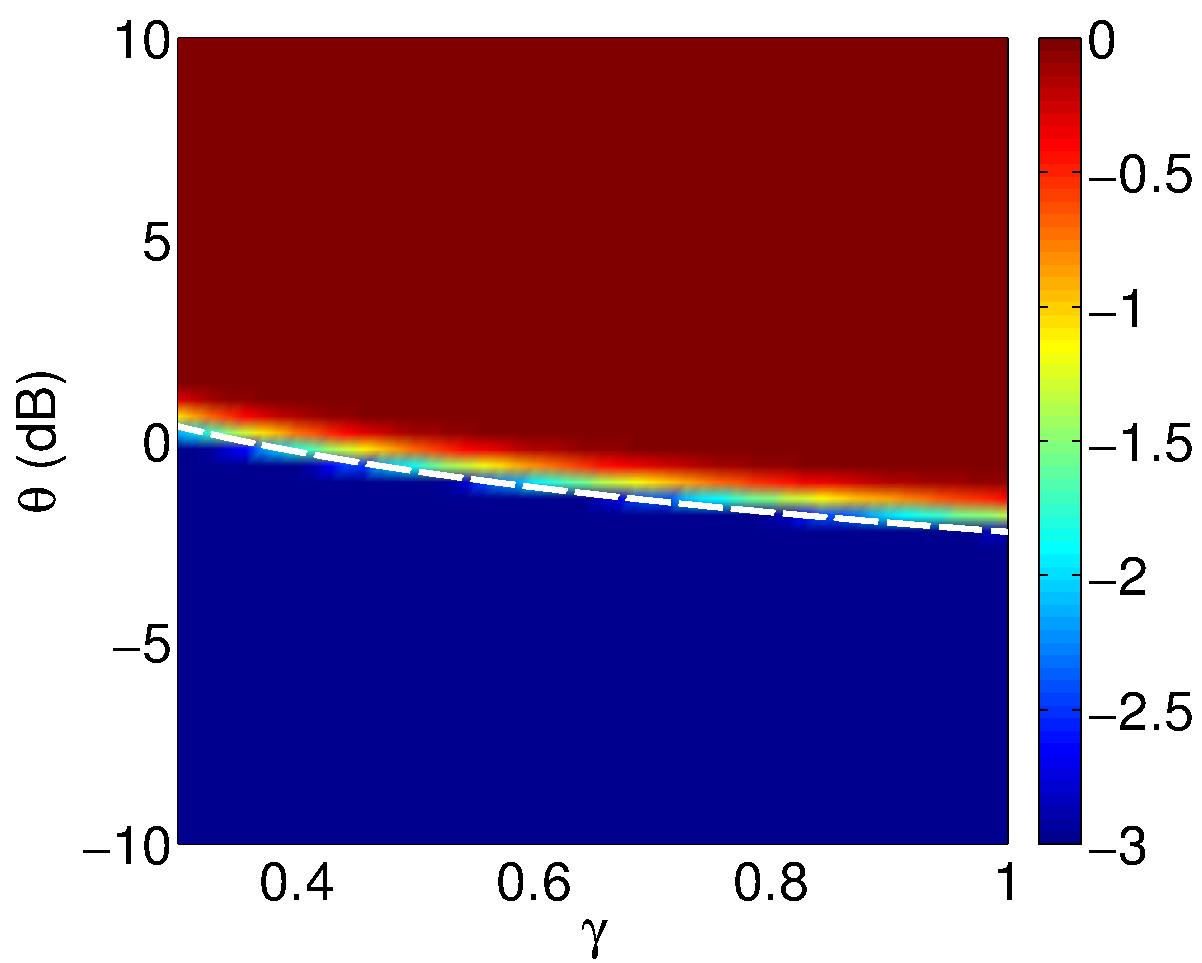
\includegraphics[width=0.4\textwidth]{figs/fig3d.pdf}
    }
    \caption{We generate data from (\ref{eq:chpt4:data_model_miss}) for $p=q=150$,
      $\kx=\ky=1$, $k=1$, $n=1200$, and various $\rho=\Pxy$ and sweep over $\theta =
      \tx_1=\ty_1$ and $\gamma=\gamma_x=\gamma_y$. We compute $\kxhat$ and $\kyhat$ as
      using Algorithm 2 of \cite{nadakuditi2010fundamental} for a significance value of
      $\alpha=0.01$. Using these estimates, we compute $\rhohatcca^{(1)}$ as the largest
      singular value of $\Cccahat$ as in (\ref{eq:chpt4:rhohatcca}) and
      $\rhohaticca^{(1)}$ as the largest singular value of $\Ciccahat$ as in
      (\ref{eq:chpt4:rhohaticca}). We then estimate the number of correlated signals
      $\khatcca$ and $\khaticca$ via (\ref{eq:chpt4:khats}) for a significance level of
      $\alpha=0.01$. We repeat this for 10000 trials and compute the percentage of trials
      where $\khatcca=1$ and $\khaticca=1$. We plot $\log_{10}$ of these percentages for
      multiples values of $\theta$ and $n$. We plot the theoretical performance limit of
      empirical CCA (given in Conjecture \ref{conj:cca_missing}) in a solid white line and
      the theoretical performance boundary of ICCA (given in Theorem
      \ref{th:missing_data}) in a dashed white line.}
    \label{fig:chpt4:cca_missing_75}
  \end{center}
\end{figure*}

\subsection{Controlled Flashing Lights Experiment}

To verify the effectiveness of ICCA for real world applications, we conducted a controlled
experiment consisting of 5 stationary flashing lights and two stationary iPhone
cameras\footnote{For a video demonstration of this experiment, visit
  \texttt{https://www.youtube.com/watch?v=WYlC2XgBDXs}. For similar experiments on an
  audio-audio dataset, visit \texttt{https://www.youtube.com/watch?v=lQzO10S7PEs} and an
  audio-video dataset visit\\ \texttt{https://www.youtube.com/watch?v=8E83P-\_oVgg}.}. Figure
\ref{fig:chpt4:flashing_sources} shows the left and right camera views at one time point
of our experiment and manually identifies each source. The 5 sources are a blue flashing
police light (BPL) outlined in the green rectangle, one phone with a flashing strobe light
(PH1) outlined in the dark blue rectangle, another phone with a flashing strobe light
(PH2) outlined in a red rectangle, a tablet with a flashing screen (T1) outlined in the
magenta rectangle, and a red flashing police light (RPL) outlined in the cyan
rectangle. From left to right, the left camera can see BPL, PH1, and PH2. From left to
right, the right camera can see PH2, T1, and RPL. Therefore, both cameras share the common
signal of PH2.

\begin{figure}
  \begin{center}
    \subfigure[Left Camera]{
      \label{fig:chpt4:flashing_left}
      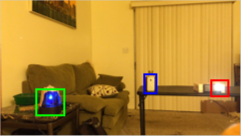
\includegraphics[width=0.47\textwidth]{figs/fig4a.png}
    }
    \subfigure[Right Camera]{
      \label{fig:chpt4:flashing_right}
      \includegraphics[width=0.47\textwidth]{figs/fig4b.png}
    }
    \caption{Left and right camera views of our experiment with boxes manually identifying
      each source. Both cameras share a common flashing phone, outlined in a red
      rectangle. Each camera has two independent sources besides the shared flashing
      phone.}
    \label{fig:chpt4:flashing_sources}
  \end{center}
\end{figure}


To synchronize the cameras we used the RecoLive MultiCam iPhone app
\footnote{http://recolive.com/en/}. After turning on all light sources, we recorded 30
seconds of video at 30 frames per second. The resolutions of the iPhone's cameras were
both $1920\times 1080$ pixels. To post-process the video data, we first converted the
video streams to grayscale and then downsampled each spatial dimension by a factor of 8,
resulting in a resolution of $240\times 135$. We then vectorized each image and stacked
the 900 frames into data matrices, both of dimension $32400 \times 900$. Finally, we
subtract the mean from each dataset so that we may run empirical CCA and ICCA on the
zero-mean datasets, $X_{\text{left}}$ and $Y_{\text{right}}$.

First, we run principal component analysis (PCA) on $X_{\text{left}}$ and
$Y_{\text{right}}$ to identify the number of signals in each dataset. We know from our
setup that each camera has 3 independent sources. Figure \ref{fig:chpt4:flashing_svs}
plots the singular values of $X_{\text{left}}$ and $Y_{\text{right}}$. However, PCA does
not provided any information about whether the identified signals are correlated across
cameras. To identify correlated pixels between the cameras, we run empirical CCA and ICCA
after each new video frame. For frame $\ell$, we construct the $32400\times\ell$
submatrices $X_{\text{left}}^\ell$ and $Y_{\text{right}}^\ell$ by taking the matrix of the
first $\ell$ original vectorized frames and zero meaning it. We then use these matrices as
the input to empirical CCA and ICCA. Using our knowledge of 3 sources present in each
camera, we set $\kxhat=\kyhat=3$. Figure \ref{fig:chpt4:flashing_corrs} plots the top 3
correlation coefficients returned by empirical CCA and ICCA over the first 800
frames. Intuitively, empirical CCA returns perfect correlation as we have only a few
frames but a large dimension (pixels).


\begin{figure}
  \begin{center}
    \subfigure[Left camera]{
      \label{fig:chpt4:ul1}
      \includegraphics[width=0.4\textwidth]{figs/fig5a.pdf}
    }
    \subfigure[Right camera]{
      \label{fig:chpt4:ul2}
      \includegraphics[width=0.4\textwidth]{figs/fig5b.pdf}
    }
    \caption{Singular value spectra of $X_{\text{left}}$ and $Y_{\text{right}}$ for the
      flashing light experiment.}
    \label{fig:chpt4:flashing_svs}
  \end{center}
\end{figure}


\begin{figure}
  \begin{center}
    \subfigure[CCA]{
      \label{fig:chpt4:flashing_cca_corrs}
      \includegraphics[width=0.4\textwidth]{figs/fig6a.pdf}
    }
    \subfigure[ICCA]{
      \label{fig:chpt4:flashing_icca_corrs}
      \includegraphics[width=0.4\textwidth]{figs/fig6b.pdf}
    }
    \caption{(a) Top three singular values returned by empirical CCA as defined in
      (\ref{eq:chpt4:rhohatcca}) for the flashing light demonstration. As we are in the
      sample deficient regime, these singular values are deterministically 1. (b) Top
      three singular values returned by ICCA as defined in (\ref{eq:chpt4:rhohaticca}) for
      the flashing light demonstration. ICCA correctly identifies two sources of
      correlation.}
    \label{fig:chpt4:flashing_corrs}
  \end{center}
\end{figure}

Using these singular values returned by empirical CCA and ICCA, we can set a threshold via
(\ref{eq:chpt4:taus}) to determine which ones indicate the presence of a correlated signal
between the datasets. Examining Figure \ref{fig:chpt4:flashing_corrs}, we can easily
accomplish this for ICCA as the top two singular values separate from the third. However,
as we operate in the sample deficient regime, we cannot set such a threshold for empirical
CCA to detect the presence of correlated signals. We overlay the thresholded unit-norm
canonical vectors (defined in (\ref{eq:chpt4:cca_vects}) and (\ref{eq:chpt4:icca_vects})) onto
the original images in Figure \ref{fig:chpt4:flashing_cca} for both empirical CCA and
ICCA. From this figure, we observe that the empirical CCA canonical vectors appear to be
very random and noisy. The ICCA canonical vectors correctly identify both sources of
correlation in our dataset.

\begin{figure}
  \begin{center}
    \subfigure[Left Camera - empirical CCA]{
      \label{fig:chpt4:flashing_left_cca}
      \includegraphics[width=0.4\textwidth]{figs/fig7a.png}
    }
    \subfigure[Right Camera - empirical CCA]{
      \label{fig:chpt4:flashing_right_cca}
      \includegraphics[width=0.4\textwidth]{figs/fig7b.png}
    }
    \subfigure[Left Camera - ICCA]{
      \label{fig:chpt4:flashing_left_icca}
      \includegraphics[width=0.4\textwidth]{figs/fig7c.png}
    }
    \subfigure[Right Camera - ICCA]{
      \label{fig:chpt4:flashing_right_icca}
      \includegraphics[width=0.4\textwidth]{figs/fig7d.png}
    }
    \caption{(a)-(b) Top 3 threholded empirical CCA canonical vectors overlayed on the
      original scene after 800 frames as computed in (\ref{eq:chpt4:cca_vects}). The red
      pixels correspond to the vector with the highest correlation, the green pixels
      correspond to the vector with the second highest correlation, and the blue pixels
      correspond to the vector with the third highest correlation in Figure
      \ref{fig:chpt4:flashing_cca_corrs}. We use a threshold of $\log(p)/\sqrt{p}$ where
      $p=32400$ pixels. (c)-(d) Top 2 threholded ICCA canonical vectors overlayed on video
      after 800 frames as computed in (\ref{eq:chpt4:icca_vects}). The red pixels
      correspond to the vector with the highest correlation and the green pixels
      correspond to the vector with the second highest correlation in Figure
      \ref{fig:chpt4:flashing_icca_corrs}. We again use a threshold of $\log(p)/\sqrt{p}$
      where $p=32400$ pixels.}
    \label{fig:chpt4:flashing_cca}
  \end{center}
\end{figure}

Given that our experiment setup has only one shared flashing light, it is initially
surprising that ICCA returns a two large singular values. Examining the ICCA canonical
vector overlay in Figure \ref{fig:chpt4:flashing_cca}, we observe that this correlation
corresponds to RPL and BPL. Figure \ref{fig:chpt4:flashing_v} examines the right singular
vectors returned by PCA corresponding to RPL and BPL. We observe that these light sources
have approximately the same period and even though they were started at random times, they
are in approximate antiphase, making them correlated. This is especially interesting
because neither camera can see both sources, but ICCA is still able to reveal a latent
correlation inherent in the period and phase of these lights.

\begin{figure}
  \begin{center}
      \includegraphics[width=0.4\textwidth]{figs/fig8.pdf}
    \caption{A portion of the right singular vectors of $X_{\text{left}}$ (blue) and
      $Y_{\text{right}}$ (red) corresponding the flashing police lights in each camera
      view. Both sources have very similar periods and are approximately in antiphase. }
    \label{fig:chpt4:flashing_v}
  \end{center}
\end{figure}

\subsection{Controlled Flashing Lights with Missing Data}

Using the same dataset in the previous section, we add missing data to each frame
independently\footnote{For a video demonstration of this experiment, please visit \texttt{https://www.youtube.com/watch?v=vhi3T4S8riE}}. We set $\gamma=\gamma_x=\gamma_y=0.75$ so that about 25\% of the pixels are
set to 0. We generate the missing pixels independently for each camera and for each
frame. We then process the data exactly as above without missing data. We note that in
this setup, our light sources do not obey the low-coherence condition, but we still run
ICCA to demonstrate its robustness. Particularly, source PH1 occupies only a small number
of pixels so that it has a very spiked signal and violates the low-coherence assumption
the most. In this missing data framework, PCA cannot detect this source. However, this
source is independent of all other signals as so we will still be able to detect all
correlated signal in the setting of Theorem \ref{th:missing_data}.

Figure \ref{fig:chpt4:flashing_cca_miss} overlays the thresholded canonical vectors
(defined in (\ref{eq:chpt4:cca_vects}) and (\ref{eq:chpt4:icca_vects})) corresponding to the
top 2 singular values for both empirical CCA and ICCA after 800 frames. Unsurprisingly,
empirical CCA is still unable to detect the two correlated signals because in this regime
the top singular values are deterministically one and the corresponding canonical vectors
are uninformative. However, ICCA is able to detect our correlated signals even in the
presence of missing data. The colored pixels clearly identify our two sources
of correlation.

\begin{figure}
  \begin{center}
    \subfigure[Left Camera - empirical CCA]{
      \label{fig:chpt4:flashing_left_cca}
      \includegraphics[width=0.4\textwidth]{figs/fig9a.png}
    }
    \subfigure[Right Camera - empirical CCA]{
      \label{fig:chpt4:flashing_right_cca}
      \includegraphics[width=0.4\textwidth]{figs/fig9b.png}
    }
    \subfigure[Left Camera - ICCA]{
      \label{fig:chpt4:flashing_left_icca_miss}
      \includegraphics[width=0.4\textwidth]{figs/fig9c.png}
    }
    \subfigure[Right Camera - ICCA]{
      \label{fig:chpt4:flashing_right_icca_miss}
      \includegraphics[width=0.4\textwidth]{figs/fig9d.png}
    }
    \caption{(a)-(b) Top 2 threholded empirical CCA canonical vectors overlayed on missing
      data video as computed in (\ref{eq:chpt4:cca_vects}). Again we use the threshold
      $\log(p)/\sqrt{p}$ for $p=32400$. The red pixels correspond to the vector with the
      highest correlation and the green pixels correspond to the vector with the second
      highest correlation in Figure \ref{fig:chpt4:flashing_cca_miss_svs}. (c)-(d) Top 2
      threholded ICCA canonical vectors overlayed on missing data video as computed in
      (\ref{eq:chpt4:icca_vects}). Again we use the threshold $\log(p)/\sqrt{p}$ for
      $p=32400$. The red pixels correspond to the vector with the highest correlation and
      the green pixels correspond to the vector with the second highest correlation in
      Figure \ref{fig:chpt4:flashing_cca_miss_svs}. For all figures,
      $\gamma_x=\gamma_y=0.75$ so that 25\% of our pixels are missing. We note that the
      middle source of the left camera violates the low-coherence assumption in Assumption
      \ref{assum:chpt4:coher} and so Theorem \ref{th:missing_data} and Conjecture
      \ref{conj:cca_missing} provide no guarantees for detecting correlations based on
      this source. }
    \label{fig:chpt4:flashing_cca_miss}
  \end{center}
\end{figure}

Figure \ref{fig:chpt4:flashing_corrs_miss} plots the top 3 singular values returned by
empirical CCA and ICCA. Unsurprisingly, the singular values reported by CCA are 1 and
uninformative. However, once we collect enough frames, there are two large singular values reported
by ICCA that identify the two sources of correlation in our dataset. Similar to the above
discussion, we can set a threshold via (\ref{eq:chpt4:taus}) to determine which ones
indicate the presence of a correlated signal between the datasets.

\begin{figure}
  \begin{center}
    \subfigure[Empirical CCA]{
      \label{fig:chpt4:flashing_cca_miss_svs}
      \includegraphics[width=0.4\textwidth]{figs/fig10a.pdf}
    }
    \subfigure[ICCA]{
      \label{fig:chpt4:flashing_icca_miss_svs}
      \includegraphics[width=0.4\textwidth]{figs/fig10b.pdf}
    }
    \caption{(a) Top three singular values returned by empirical CCA as defined in
      (\ref{eq:chpt4:rhohatcca}). As we are in the sample deficient regime, these singular
      values are deterministically 1. (b) Top three singular values returned by ICCA as
      defined in (\ref{eq:chpt4:rhohaticca}). ICCA correctly identifies two sources of
      correlation. As our data matrices now have missing data, it takes more frames for
      ICCA to identify the two sources of correlations. For both figures,
      $\gamma_x=\gamma_y=0.75$ so that 25\% of our pixels are missing. This figure is
      analogous to Figure \ref{fig:chpt4:flashing_corrs}, which observes all data so that
      $\gamma_x=\gamma_y=1$.}
    \label{fig:chpt4:flashing_corrs_miss}
  \end{center}
\end{figure}

\section{Conclusion}\label{sec:chpt4:concl}

In this paper we explored the problem of detecting correlations present in exactly two
datasets when the covariance and cross-covariance matrices are unknown and estimated from
training data. We showcased that the standard algorithm, empirical CCA, fails to detect
such correlations when the number of training samples is limited. Motivated by insights
from random matrix theory, we presented informative CCA (ICCA), which can reliably detect
correlations present in low-rank-correlated-signal-plus-noise type datasets. We then
extended this analysis to the case of missing data and showcased the improved detection
performance of ICCA on both synthetic and real-world examples. 

This paper assumed a low-rank-correlated-signal-plus-noise data model, which is ubiquitous
in signal processing applications.  We note that depending on the application, the linear,
low-rank-correlated-signal-plus-noise data model may be inappropriate. In such a setting,
kernel CCA (KCCA) \cite{welling2011first,yu2007learning} uses the kernel trick to first
map the data into a higher dimensional space before running CCA. The performance analysis
of such kernel methods for non-linear data models is important future
work. Proving Conjectures \ref{conj:khat_lims}, \ref{conj:icca}, and
  \ref{conj:cca_missing} remains an open problem and important area of future
  work. Finally, in a future paper we will characterize the accuracy of the empirical
  canonical vector estimates and provide a new estimate that uses insights from random
  matrix theory.


\appendix

\section*{Proof of Proposition \ref{prop:bao}}
Bao et al. \cite{bao2014canonical} proved this result for a slightly simplified
model. Here we provide the linear transformations to recover their model. We may write our
data matrices $X$ and $Y$ jointly via,
\be
\left[\begin{array}{c}X \\ Y\end{array}\right] = \left[\begin{array}{cc}\Rxx & \Rxy \\ \Rxy^H & \Ryy\end{array}\right]^{1/2}\left[\begin{array}{c}W_1 \\ W_2\end{array}\right]
\ee
where $W_1$ is a $p\times n$ matrix with independent $\mathcal{N}(0,1)$ entries and $W_2$
is an independent $q\times n$ matrix with independent $\mathcal{N}(0,1)$. As $p+q<n$,
$\Rxx$ and $\Ryy$ are non-singular. Define
{\small \be\ba
\left[\begin{array}{c}\widetilde{X} \\ \widetilde{Y}\end{array}\right] &=
\left[\begin{array}{cc}R_{xx}^{-1/2} & 0 \\ 0 &
    R_{yy}^{-1/2}\end{array}\right]^{1/2}\left[\begin{array}{c}X \\ Y\end{array}\right] \\
&=
\left[\begin{array}{cc}I_p & \Rxx^{-1/2}\Rxy\Ryy^{-1/2}.  \\ \Ryy^{-1/2}\Rxy^H\Rxx^{-1/2}
    & I_q\end{array}\right]\left[\begin{array}{c}W_1 \\ W_2\end{array}\right].
\ea\ee}
With the definitions of the covariance matrices in (\ref{eq:chpt4:true_scm}), we have that
$\Rxx^{-1/2}\Rxy\Ryy^{-1/2}$
\be\ba
&= \Ux\left(\Tx +
  I_{\kx}\right)^{-1/2}\Tx^{1/2}\Pxy\Ty^{1/2}\left(\Ty + I_{\ky}\right)^{-1/2}\Uy^H\\
 &= \Ux\Kxytil\Uy^H.
\ea\ee
From this expression, it is clear why we defined $\Kxytil$ as we originally did. Let
$U_{\Kxytil} K V_{\Kxytil}$ be the SVD of $\Kxytil$, where $K$ is the
$\kx\times\ky$ matrix with $\kappa_j$ along the diagonal. Define $F = \left[\left(\Ux
    U_{\Kxytil}\right) \,\,\,\left(\Ux U_{\Kxytil}\right)^{\perp}\right]$ and
$G=\left[\left(\Uy V_{\Kxytil}\right)\,\,\,\left(\Uy V_{\Kxytil}\right)^{\perp}\right]$. Then
\be\ba
&\left[\begin{array}{c}\widetilde{\widetilde{X}} \\ \widetilde{\widetilde{Y}}\end{array}\right] &&=
\left[\begin{array}{cc}F^H & 0 \\ 0 &
    G^H\end{array}\right]^{1/2}\left[\begin{array}{c}\widetilde{X} \\
    \widetilde{Y}\end{array}\right] \\ &&&=  \left[\begin{array}{cc}F^HR_{yy}^{-1/2} & 0 \\ 0 &
    G^HR_{yy}^{-1/2}\end{array}\right]^{1/2}\left[\begin{array}{c} X \\
    Y \end{array}\right]\\
&&& = \left[\begin{array}{cc}I_p & K \\ K^H &
    I_q\end{array}\right]^{1/2}\left[\begin{array}{c}W_1 \\ W_2\end{array}\right].
\ea\ee
Transforming $X$ and $Y$ to $\widetilde{\widetilde{X}}$ and
$\widetilde{\widetilde{Y}}$ preserves the canonical correlation estimates because our
transformation matrix is non-singular. After this transformation, we follow the proof from
Bao et al. \cite{bao2014canonical} with $\sqrt{r_i} = \kappa_i$.

\section*{Theorem needed to prove Theorem \ref{th:v_ip}}

\begin{Th}\label{th:w_ip}
Let $\widetilde{u}_i$ and $\widetilde{v}_i$ be the left and right singular vectors
associated with the $i$-th singular value, $\widetilde{\theta}_i$, of the $p\times n$ matrix
\be
\widetilde{X} = \sum_{i=1}^{k}\underbrace{\theta_i u_iv_i^H}_{P} + X.
\ee
Assume that $X$ satisfies
the hypotheses in Assumption \ref{assum:chpt4:noise} and suppose that $\theta_i>c^{1/4}$ for
$c=p/n$. Let $w$ be an
arbitrary unit norm vector that is orthogonal to $u_i$ for some $i\in\left\{1,\dots,k\right\}$. Then as $n,p\to\infty$ such that $p/n\to c$,  we have that
\be
\left\langle w,\widetilde{u}_i\right\rangle \convas 0.
\ee
\end{Th}
\begin{proof}
  The result of this theorem may be of interest outside of this paper for analysis of
  similar low-rank signal-plus-noise matrix models. We will use this theorem to prove
  Theorem \ref{th:v_ip}. We begin with a technical lemma needed to prove the theorem.

\begin{Lem}\label{lem:mip}
Let $U=[u_1,\dots,u_k]\in\complex^{p\times k}$ and $V=[v_1,\dots,v_k]\in\complex^{n\times
  k}$ be independent matrices with orthonormal columns. Let $X\in\complex^{p\times n}$
satisfy the hypotheses in Assumption \ref{assum:chpt4:noise}. Then as $n,p\to\infty$ with $p/n\to
c$, for $i\neq j$
\be
u_i^H\left(z^2 I_n - XX^H\right)^{-1}u_j \convas 0.
\ee
Similarly, for all $i,j$,
\be
u_i^H\left(z^2 I_n - XX^H\right)^{-1}Xv_j \convas 0.
\ee
\end{Lem}
\begin{proof}
The proof of Lemma 4.1 in \cite{benaych2012singular} proves both of these statements.
\end{proof}

We now are in a position to prove Theorem \ref{th:w_ip}. If $w\in\Span(u_1,\dots,u_k)$,
then Theorem 2.10 c) of \cite{benaych2012singular}
proves our result. If $w\not\in\Span(u_1,\dots,u_k)$, then we may write
\be
w = w_u + w_u^\perp,
\ee
where $w_u\in\Span(u_1,\dots,u_k)$ and $w_u^\perp$ is in the orthocomplement of
$\Span(u_1,\dots,u_k)$. Therefore applying Theorem 2.10 c) of \cite{benaych2012singular}
\be
\left\langle w,\widetilde{u}_i\right\rangle = \left\langle w_u,\widetilde{u}_i\right\rangle
+ \left\langle w_u^\perp,\widetilde{u}_i\right\rangle \convas \left\langle w_u^\perp,\widetilde{u}_i\right\rangle,
\ee
so we only must focus on $w_u^\perp$.

Based on their definitions, $\widetilde{X}\widetilde{X}^H\widetilde{u}_i =
\widetilde{\theta}_i^2\widetilde{u}_i$ and $\widetilde{X}^H\widetilde{u}_i =
\widetilde{\theta}_i\widetilde{v}$. Using the fact that $\widetilde{X}= P+X$, we have
\beq\label{eq:chpt4:step1}
\left(PP^H + PX^H + XP^H + XX^H\right)\widetilde{u}_i = \widetilde{\theta}_i^2\widetilde{u}_i
\eeq
and $\left(X^H+P^H\right)\widetilde{u}_i =\widetilde{\theta}_i\widetilde{v}$. Multiplying
both sides of this second expression by $P$, we have
\be
PX^H\widetilde{u}_i+PP^H\widetilde{u}_i =\widetilde{\theta}_iP\widetilde{v}_i.
\ee
Substituting this expression in (\ref{eq:chpt4:step1}) gives
\be
\widetilde{\theta}_iP\widetilde{v}_i +XP^H\widetilde{u}_i + XX^H\widetilde{u}_i =
\widetilde{\theta}_i^2\widetilde{u}_i .
\ee
Rearranging terms gives
\be
\widetilde{u}_i= \left(\widetilde{\theta}_i^2I_{p} -
  XX^H\right)^{-1}\left(\widetilde{\theta}_iP\widetilde{v}_i +XP^H\widetilde{u}_i\right).
\ee
Therefore, we have the equivalences for $\langle w_u^\perp,\widetilde{u}_i\rangle$
\be\ba
&=  &&w_u^{\perp H}\left(\widetilde{\theta}_i^2I_{p} -
  XX^H\right)^{-1}\left(\widetilde{\theta}_iP\widetilde{v}_i +XP^H\widetilde{u}_i\right)\\
& = &&\widetilde{\theta}_iw_u^{\perp H}\left(\widetilde{\theta}_i^2I_{p} -
  XX^H\right)^{-1}\sum_{j=1}^k\theta_j\langle v_j,\widetilde{v}_i\rangle u_j \\
&&&+
\widetilde{\theta}_iw_u^{\perp H}\left(\widetilde{\theta}_i^2I_{p} -
  XX^H\right)^{-1}X\sum_{j=1}^k\theta_j\langle u_j,\widetilde{u}_i\rangle v_j. \\
\ea\ee
By Theorem 2.7 c) in \cite{benaych2012singular}, we have that for $i\neq j$, $|\langle u_j,
\widetilde{u}_i\rangle|\convas 0 $ and $|\langle v_j, \widetilde{v}_i\rangle|\convas 0$. Therefore
\beq\label{eq:chpt4:w_thm_main}\ba
& \langle w_u^\perp,\widetilde{u}_i\rangle = &&\left(\widetilde{\theta}_i\theta_i\langle
  v_i,\widetilde{v}_i\rangle\right)w_u^{\perp H}\left(\widetilde{\theta}_i^2I_{p} -
  XX^H\right)^{-1} u_i \\
&&&+ \left(\widetilde{\theta}_i\theta_i\langle
  u_i,\widetilde{u}_i\rangle\right)w_u^{\perp H}\left(\widetilde{\theta}_i^2I_{p} -  XX^H\right)^{-1}X v_i. \\
\ea\eeq
By Lemma \ref{lem:mip},
\be
w_u^{\perp H}\left(\widetilde{\theta}_i^2I_{p} -  XX^H\right)^{-1} u_i\convas 0
\ee
and
\be
w_u^{\perp H}\left(\widetilde{\theta}_i^2I_{p} -  XX^H\right)^{-1}X v_i\convas 0.
\ee
Therefore, $\langle w_u^\perp,\widetilde{u}_i\rangle\convas 0$.
\end{proof}

\section*{Proof of Theorem \ref{th:v_ip}}
The entries of the matrix $\Vxcir^H\Vycir$ are the inner products between the columns of $\Vxcir$ and $\Vycir$
\be
\left|\left(\Vxcir^H\Vycir\right)\right|_{ij} = \left|\Vxcir^H(:,i)\Vycir(:,j)\right|.
\ee
Notice that we may write
\beq\label{eq:chpt4:v_orth}\ba
&\Vxcir(:,i) = a \Vy(:,j) + b w_y\\
&\Vy(:,j) = \kxy_{ij}\Vx(:,i) + c w_x
\ea\eeq
for some arbitrary unit-norm vector $w_x$ that is orthogonal to $\Vx(:,i)$, some arbitrary
unit-norm vector $w_y$ that is orthogonal to $\Vy(:,j)$, and constants $a$, $b$, and $c$. With
these observations, we have
\be\ba
& \Vxcir^H(:,i)\Vycir(:,j) && = \left(a \Vy(:,j) + b w_y\right)^H\Vycir(:,j)\\
&&& = a \Vy^H(:,j)\Vycir(:,j) + b w_y^H\Vycir(:,j).\\
\ea\ee
By Theorem \ref{th:w_ip}, $w_y^H\Vycir(:,j)\convas0$. As derived in theorem 5.2 in
\cite{nadakuditi2011fundamental},
{\small \be
\left|\Vy^H(:,j)\Vycir(:,j)\right|\convas\alpha_{y,j}\defeq\begin{cases} \sqrt{1 - \frac{c_y + \ty_j}{\ty_j(\ty_j + c_x)}} &
  \ty_j > c^{1/4} \\ 0 & \text{otherwise} \end{cases}.
\ee}
Therefore, $\left|\Vxcir^H(:,i)\Vycir(:,j)\right|\convas a\alpha_{y,j}$. Using the expression for
$\Vxcir(:,i)$ in (\ref{eq:chpt4:v_orth}), we observe that
\be
\Vy(:,j)^H\Vxcir(:,i) = a.
\ee
Using the expression for $\Vy(:,j)$ in (\ref{eq:chpt4:v_orth}), we have
\be\ba
& a  && = \Vy(:,j)^H\Vxcir(:,i)\\
&&& = \left(\kxy_{ij}\Vx(:,i) + c w_x\right)^H\Vxcir(:,i)\\
&&& = \kxy_{ij}\Vx^H(:,i)\Vxcir(:,i) + c w_x^H\Vxcir(:,i).\\
\ea\ee
By Theorem \ref{th:w_ip}, $w_x^H\Vxcir(:,i)\convas0$. As derived in theorem 5.1 of
\cite{nadakuditi2011fundamental},
{\small \be
\left|\Vy(:,j)\Vycir(:,j)\right|\convas\defeq\alpha_{x,i}\begin{cases} \sqrt{1 - \frac{c_x + \tx_i}{\tx_i(\tx_i + c_x)}} &
  \tx_i > c^{1/4} \\ 0 & \text{otherwise} \end{cases}.
\ee}
Therefore, $|a|\convas\left|\kxy_{ij}\right|\alpha_{x,i}$. Therefore,
\be
\left|\Vxcir^H(:,i)\Vycir(:,j)\right|\convas \left|\kxy_{ij}\right|\alpha_{x,i}\alpha_{y,i}.
\ee


\section*{Proof of Theorem \ref{th:khat_lims}}
For ICCA, recall that
\be
\khaticca = \sum_{i=1}^{\min(\kxhat,\kyhat)}
\indicator_{\left\{\left(\rhohaticca^{(i)}\right)^2 >\tauicca\right\}}.
\ee
When $\kxhat=\kx$ and $\kyhat=\ky$, the estimate of the number of correlated signals becomes
\be
\khaticca \convas \sum_{i=1}^{\min(\kx,\ky)} \indicator_{\left\{\left(\rhohaticca^{(i)}\right)^2 >\tauicca\right\}}.
\ee
To prove the theorem, we want to show that
\be
\rhohaticca^{(k)} > 0 \text{ almost surely},
\ee
under the conditions on $\Tx$ and $\Ty$ in the theorem statement. Momentarily, we assume that
$k=\min(\kx,\ky)$. The singular values of $\Vxcir^H\Vycir$ are
ordered and so we must show that 
\be
 \left(\rhohaticca^{(\min(\kx,\ky))}\right)^2 >\tauicca \text{ almost surely.}
\ee
From Theorem \ref{th:v_ip}, we also know that
\be
\left|\left[\Vxcir^H\Vycir\right]_{ij}\right| \convas\left|\kxy_{ij}\right|\alpha_{x,i}\alpha_{y,i}.
\ee
Using this fact we define
\be\ba
&A_x = \diag(\alpha_{x,1},\dots,\alpha_{x,\kx})\\
&A_y=\diag(\alpha_{y,1},\dots,\alpha_{y,\ky})\\
\ea\ee
so that we may write
\be
\Vxcir^H\Vycir = A_x\Kxy A_y + \Delta,
\ee
where $\Delta = [\delta_{ij}]$ such that $\delta_{ij} \convas 0$. Examining (\ref{eq:chpt4:alphas}), we see that under the above conditions on $\Tx$ and $\Ty$,
$A_x$ and $A_y$ are both full rank. Define
\be\ba
&\alpha_{x,\text{min}} = \min_{i=1\dots,\kx}\alpha_{x,i}\\
&\alpha_{y,\text{min}} = \min_{i=j\dots,\ky}\alpha_{y,j}.\\
\ea\ee
By properties of singular values
\be\ba
&\sigma_{\min}(A_x\Kxy A_y) - \sigma_{\max}(\Delta) &&\leq &&&\sigma_{\min}(A_x\Kxy A_y +
\Delta)\\ &&&\leq &&&\sigma_{\min}(A_x \Kxy A_y) \\ &&&&&&+ \sigma_{\max}(\Delta).
\ea\ee
Examining $\sigma_{\max}(\Delta)$, we observe that
\be
\sigma_{\max}(\Delta) \leq \|\Delta\|_F = \sqrt{\sum_{i=1}^{\kx} \sum_{j=1}^{\ky} \left|\delta_{ij}\right|^2}.
\ee
Using the fact that $\delta_{ij}\convas 0$, we have that $\sigma_{\max}(\Delta)\convas
0$. Therefore, almost surely
\be
\sigma_{\min}(A_x\Kxy A_y) \leq \sigma_{\min}(A_x\Kxy A_y +
\Delta)\leq \sigma_{\min}(A_x \Kxy A_y),
\ee
which implies that
\be
\rhohaticca^{(\min(\kx,\ky))}\convas\sigma_{\min}(A_x \Kxy A_y)
\ee
By properties of singular values
\be\ba
&\rhohaticca^{(\min(\kx,\ky))} && = \sigma_{\min(\kx,\ky)}\left(\Vxcir^H\Vycir\right)\\
&&& \convas \sigma_{\min(\kx,\ky)}\left(A_x\Kxy A_y\right)\\
&&& \geq \sigma_{\kx}\left(A_x\right)\sigma_{\min(\kx,\ky)}
\left(\Kxy\right)\sigma_{\ky}\left(A_y\right)\\
&&& = \alpha_{x,\text{min}}\kappa_{\min(\kx,\ky)}\alpha_{y,\text{min}} > 0,\\
\ea\ee
and we have proved the desired result.

\begin{comment}
Next we turn to our statistical test in the asymptotic setting. Unlike $\Cccahat$, whose
dimension scales with $n$, the dimension of $\Ciccahat$ remains $\kx\times\ky$ even as $n$
increases. Therefore, in the null setting as $n\to\infty$ the entries $\Ciccahat$ converge
almost surely to 0. Therefore, in the asymptotic setting our test becomes
\be
\khaticca = \sum_{i=1}^{\min(\kx,\ky)} \indicator_{\left\{\left(\rhohaticca^{(i)}\right)^2 >0\right\}}.
\ee
Therefore,
\be\ba
&\Prob{\left(\khaticca = k\right)} &&= \Prob{\left(\rhohaticca^{(\min(\kx,\ky))}\right)^2
  > 0 }\\
&&& \geq \Prob{\left(\alpha_{x,\text{min}}\kappa_{\min(\kx,\ky)}\alpha_{y,\text{min}}\right)^2  > 0 }\\
&&& \to 1.\\
\ea\ee
The last equality comes from the fact that under our conditions on $\Tx$ and $\Ty$,
the $\alpha$ terms are non-zero and from the fact that we momentarily assumed
$k=\min(\kx,\ky)$ so that $\kappa_{\min(\kx,\ky)}$ is non-zero. We note that this holds
for all significance levels.

Lastly, we argue that the above analysis holds when $k<\min(\kx,\ky)$. In this setting,
the last $\min(\kx,\ky)-k$ singular values of $A_y\Kxy A_y$ are zero. The above
analysis holds for the largest $k$ canonical correlations, showing that they are non-zero
in the asymptotic limit. Therefore, the asymptotic statistic will correctly mark these top $k$
singular values as an indicator of the $k$ correlations and correctly identify the
smallest $\min(\kx,\ky)-k$ singular values as not containing correlation as they are zero
in the asymptotic limit.
%Therefore,
%\be
%\Prob{\khaticca = k} \geq
%\Prob{\left(\alpha_{x,\text{min}}\kappa_{\min(\kx,\ky)}\alpha_{y,\text{min}}\right)^2 > \tauicca}.
%\ee
%Finally we examine $\tauicca$ when $p,q,n\to\infty$ with $p/n\to c_x$, $q/n\to c_y$ and
%$\kx$ and $\ky$ fixed. In the equations for $\mu_{\kx,\ky,n}$, we see that in this
%asymptotic setting, $\gamma\to 0$ and $\varphi\to 0$. Therefore
%$\mu_{\kx,\ky,n}\to\log(0)=-\infty$. Similarly, $\sigma_{\kx,\ky,n}\to c_\sigma$ for some
%finite $c_\sigma$ dependent on $\kx$ and $\ky$. Therefore, for all values of $\alpha$,
%\be
%\tauicca\to-\infty.
%\ee
%Therefore
%\be\ba
%&\Prob{\khaticca = k} &&\geq
%\Prob{\left(\alpha_{x,\text{min}}\kappa_{\min(\kx,\ky)}\alpha_{y,\text{min}}\right)^2 >
%  \tauicca}\\
%&&& \convas \Prob{\left(\alpha_{x,\text{min}}\kappa_{\min(\kx,\ky)}\alpha_{y,\text{min}}\right)^2 >
%  -\infty}
%&&& = 1.
%\ea\ee
%As $\alpha_{x,\text{min}}$, $\alpha_{y,\text{min}}$ and $\kappa_{\min(\kx,\ky)}$ are
%constant when $p,q,n\to\infty$ with $p/n\to c_x$, $q/n\to c_y$ and
%$\kx$ and $\ky$ fixed, we have that
%\be
%\Prob{\khaticca=k}\convas 1.
%\ee

\end{comment}

\section*{Proof of Theorem \ref{th:missing_data}}
Defining $P_x=\Ux\Vx^H$ We may write (\ref{eq:chpt4:data_model_miss}) as
\be\ba
& X &&= \underbrace{P_x\odot M_x}_{\widehat{P}_x} + \underbrace{Z_x\odot
  M_x}_{\widehat{Z}_x}\\
&&& = \E{\widehat{P}_x} + \widehat{Z}_x + \Delta_{\widehat{P}_x}\\
&&& = \underbrace{\gamma_x P_x + \widehat{Z}_x}_{\widetilde{X}} + \Delta_{\widehat{P}_x}.\\
\ea\ee
Similarly, we may write $Y=\widetilde{Y} + \Delta_{\widehat{P}_y}$ where $\widetilde{Y} =
\gamma_y P_y + \widehat{Z}_y$.

First we show that the maximum singular value of $\Delta_{\widehat{P}_x}$ and
$\Delta_{\widehat{P}_y}$ converge almost surely to 0. Under the low-coherence assumption,
we have that
\beq\ba\label{eq:chpt4:P}
&\max_{ij}|P_x|_{ij}&&\leq \max_{i}\tx_i\max_{k}\|u_k^{(x)}\|_\infty\max_{\ell}\|v_\ell^{(x)}\|_\infty\\ &&&=
  \max_{i}\tx_i\mathcal{O}\left(\frac{\text{log } n,p \text{ factors}}{\sqrt{np}}\right).
\ea\eeq
By assumption that $c_x>0$, we have that $n=\mathcal{O}(p)$. This fact, coupled with the
fact that $\tx_i$ is not dependent on $n$ gives
\beq\label{eq:chpt4:P_2}
\max_{ij}|P_x|_{ij}\leq \mathcal{O}\left(\frac{\text{log } n \text{ factors}}{n}\right).
\eeq
To characterize the largest singular value of $\Delta_{\widehat{P}_x}$, we want to use
Latala's theorem \cite{latala2005some}, which states that for a matrix $A$ with
independent mean zero random entries with bounded fourth moment
\be\ba
&\E{\sigma_1\left(A\right)} \leq
&&C\left[\max_i\left(\sum_j\E{A_{ij}^2}\right)^{1/2}\right . \\
  &&& +
    \max_j\left(\sum_i\E{A_{ij}^2}\right)^{1/2} \\
&&&\left . + \left(\sum_{i,j}\E{A_{ij}^4}\right)^{1/4}\right]
\ea\ee
for some universal constant $C$ that does not depend on $n$ or $p$. Through basic
calculation, one can show that
\be\ba
& \E{\left(\Delta_{\widehat{P}_x}\right)_{ij}^2} = \gamma_x\left(1-\gamma_x\right)\left(P_x\right)_{ij}^2\\
&\E{\left(\Delta_{\widehat{P}_x}\right)_{ij}^4} = \left(-3\gamma_x^4+6\gamma_x^3 -
  4\gamma_x^2 + \gamma\right)\left(P_x\right)_{ij}^4.\\
\ea\ee
These expressions satisfy the conditions on Latala's theorem. Therefore, by substituting
these expressions into Latala's theorem with the bound in (\ref{eq:chpt4:P_2}), we have
\be
\E{\sigma_1\left(\Delta_{\widehat{P}_x}\right)}\leq\mathcal{O}\left(\frac{\text{log } n \text{ factors}}{\sqrt{n}}\right).
\ee
By concentration and convexity of the largest singular value (see
\cite{nadakuditi2014optshrink} page 3015), we have that in our
asymptotic regime
\be
\sigma_1(\Delta_{\widehat{P}_x})\convas 0.
\ee
Using a similar argument
\be
\sigma_1(\Delta_{\widehat{P}_y})\convas 0.
\ee
Therefore we have that
\be\ba
&X\to \gamma_x P_x + \widehat{Z}_x\\
&Y\to\gamma_y P_y + \widehat{Z}_y.\\
\ea\ee
Examining $\widehat{Z}_x$, we have
\be\ba
&\E{\widehat{Z}_{ij}^{(x)}} =
&&\E{\widehat{Z}_{ij}^{(x)}|M_{ij}^{(x)}=0}\Prob{M_{ij}^{(x)}=0} \\
&&&+
\E{\widehat{Z}_{ij}^{(x)}|M_{ij}^{(x)}=1}\Prob{M_{ij}^{(x)}=1} = 0
\ea\ee
and
\be\ba
\E{\left(\widehat{Z}_{ij}^{(x)}\right)^2} &=
&&\E{\left(\widehat{Z}_{ij}^{(x)}\right)^2|M_{ij}^{(x)}=0}\Prob{M_{ij}^{(x)}=0}+ \\
&&&
\E{\left(\widehat{Z}_{ij}^{(x)}\right)^2|M_{ij}^{(x)}=1}\Prob{M_{ij}^{(x)}=1}\\
& = &&0 + \gamma_x.
\ea\ee
Therefore, $\widehat{Z}_{ij}^{(x)}$ are i.i.d. zero mean with variance
  $\gamma_x$ and $\widehat{Z}_x\to\sqrt{\gamma_x}Z_x$. Using this observation,
\be\ba
&X &&\convas \gamma_x P_x + \widehat{Z}_x\\
&&& \to \gamma_x P_x + \sqrt{\gamma_x}Z_x\\
&&& = \sqrt{\gamma_x}\left(\sqrt{\gamma_x} P_x + Z_x\right).\\
\ea\ee
Similarly, $Y\to\sqrt{\gamma_y}\left(\sqrt{\gamma_y} P_y + Z_y\right)$.

From this we can conclude that eigenvector expressions of the form $\langle u, \widehat{u}\rangle$
behave as if we replace $\Tx$ with $\gamma_x\Tx$ and $\Ty$ with $\gamma_y\Ty$. Consider
\beq\label{eq:chpt4:ip_missing_orig}\ba
&\left|u_i^H\left(zI - (Z_x + \Delta_{\widehat{P}_x}) \right. \right .&&\left . (Z_x +
  \Delta_{\widehat{P}_x})^H\right)^{-1} \cdot \\  &&& \left. u_j - u_i^H\left(zI - Z_xZ_x^H\right)^{-1}u_j
\right|,
\ea\eeq
which as a consequence of the variational characterization of the largest singular value
is upper bounded by
{\small \beq\label{eq:chpt4:ip_missing}
\sigma_1\left(\left(zI - (Z_x + \Delta_{\widehat{P}_x})(Z_x +
  \Delta_{\widehat{P}_x})^H\right)^{-1} -\left(zI - Z_xZ_x^H\right)^{-1}\right).
\eeq}
Following a similar argument in \cite{nadakuditi2014optshrink} (equation 34), we have that (\ref{eq:chpt4:ip_missing}) is upper
bounded by
\be
\frac{3\sigma_z(Z_x)}{\Im w}\sigma_1(\Delta_{\widehat{P}_x}),
\ee
where $\Im w>0$. Using the facts that $\sigma_1(Z_x)\convas \sqrt{\gamma_x} b_x$ by the
above relationship and $\sigma_1(\Delta_{\widehat{P}_x})\convas 0$ combined with  Assumption \ref{assum:chpt4:noise}, we have that (\ref{eq:chpt4:ip_missing_orig})
converges to 0. Using a similar argument, one can prove the same result for quadratic
forms with $Z_y$ and $\Delta_{\widehat{P}_y}$.

Therefore, an analogous version of Theorem \ref{th:w_ip} holds for the missing data
section, as the quadratic forms used by Lemma \ref{lem:mip} still hold. Therefore, we
prove the theorem following the same rank argument as Theorem \ref{th:khat_lims}, except
that we replace $\Tx$ with $\gamma_x\Tx$ and replace $\Ty$ with $\gamma_y\Ty$.


\chapter{On Estimating Population Canonical Vectors}\label{sec:chpt_cca_vects}
\section{Introduction}

In Chapter \ref{sec:chpt_cca_det}, we presented statistical tests for empirical CCA and
informative CCA. This analysis showed that in the sample deficient regime, the canonical
correlations returned by ICCA can reliably detect the presence of correlated signals
between two datasets. In this chapter, we complete the analysis of empirical CCA and ICCA
by examining the accuracy of the canonical vectors associated with the canonical
correlations.

Using the same data model as Chapter \ref{sec:chpt_cca_det}, we begin by deriving the CCA
population canonical vectors if all parameters are known. From this analysis we see that
the canonical vectors are a linear combination of signal vectors that form the linear
subspace of each dataset. This linear combination involves the eigen-structure of the
cross-correlation matrix and the inverse signal-to-noise ratios (SNRs) of the individual
correlation matrices. We show that the canonical vectors returned by empirical CCA are
very inaccurate in the low-sample, low-SNR regime while the canonical vectors returned by
ICCA are able to properly estimate the true population canonical vectors in this regime.

This analysis of the canonical vector accuracy leads to some nice observations. First, we
notice that the canonical vector estimation is very sensitive to the estimation of the
underlying SNRs since we need to use their inverses. With this observation in mind, we
form an asymptotically optimal estimator, which we call \iccap, that provides an optimal
linear combination of the estimated components of the signal subspaces, where these
weights incorporate the accuracy each component of the estimated signal subspace. These
weights make contact with the accuracy of subspace components that we used in Chapters
\ref{sec:chpt_msd} and \ref{sec:chpt_msd_exten} to improve matched subspace detection. We
finally consider an orthogonal estimate to the canonical vectors and discuss when this
estimate is equivalent to ICCA and \iccap.

\subsection{Data Model}

We use the same data model in Chapter \ref{sec:chpt_cca_det}, but repeat it here to
facilitate exposition. Let $\xii\in\complex^{p\times 1}$ and $\yii\in\complex^{q\times 1}$ be
modeled as
\beq\ba\label{eq:chpt5:data_model}
&\xii = \Ux\sx + \zx\\
&\yii = \Uy\sy + \zy,\\
\ea\eeq
where $\Ux^H\Ux=I_{\kx}$, $\Uy^H\Uy=I_{\ky}$, $\zx\simiid\mathcal{CN}(0,I_p)$ and
$\zy\simiid\mathcal{CN}(0,I_q)$. Furthermore, assume that
\be\ba
&\sx\sim\mathcal{CN}(0,\Tx)\\
&\sy\sim\mathcal{CN}(0,\Ty),\\
\ea\ee
where $\Tx=\diag\left(\left(\tx_1\right)^2,\dots,\left(\tx_{\kx}\right)^2\right)$ and
$\Ty=\diag\left(\left(\ty_{1}\right)^2,\dots,\left(\ty_{\ky}\right)^2\right)$. Assume that
$\zx$ and $\zy$ are mutually independent and independent from both $\sx$ and
$\sy$. Finally, assume that 
\be
\E{\sx \sy^H} \defeq \Kxy = \Tx^{1/2}\Pxy\Ty^{1/2}
\ee
where the entries of $\Pxy$ are $-1\leq \rho_{kj} \leq 1$ and represent the correlation
between $\sx^{(k)}$ and $\sy^{(j)}$. For reasons to be made clear later, define 
\be
\Kxytil = \left(\Tx+I_{\kx}\right)^{-1/2}\Kxy\left(\Ty+I_{\ky}\right)^{-1/2}
\ee
and define the singular values of $\Kxytil$ as
$\kappa_1,\dots,\kappa_{\min(\kx,\ky)}$. Under this model, we define the following 
covariance matrices  
\beq\label{eq:chpt5:true_scm}\ba
&\E{\xii\xii^H} = \Ux\Tx\Ux^H + I_p \defeq \Rxx\\
&\E{\yii\yii^H} = \Uy\Ty\Uy^H + I_q \defeq \Ryy\\
&\E{\xii\yii^H} = \Ux\Kxy\Uy^H \defeq \Rxy.\\
\ea\eeq

Finally, define the random matrices $Z_n^x$ and $Z_n^y$  formed by stacking $n$
realizations of $\zx$ and $\zy$ columnwise via
\be\ba
& Z_n^x = \left[z_{x,1},\dots, z_{x,n}\right]\\
& Z_n^y = \left[z_{y,1},\dots, z_{y,n}\right].
\ea\ee
Denote the singular values of these matrices as 
\be\ba
&\sigma_1(Z_n^x)\geq\cdots\geq\sigma_p(Z_n^x)\\
&\sigma_1(Z_n^y)\geq\cdots\geq\sigma_q(Z_n^y)\\
\ea\ee
where without loss of generality we let $p<n$ and $q<n$ to simplify the definition of the
empirical singular value distribution. Let $\mu_{Z_n^x}$ and $\mu_{Z_n^y}$ be the
empirical singular value distribution defined as
\be\ba
&\mu_{Z_n^x} = \frac{1}{p}\sum_{i=1}^p\delta_{\sigma_i(Z_n^x)}\\
&\mu_{Z_n^y} = \frac{1}{q}\sum_{i=1}^q\delta_{\sigma_i(Z_n^y)}\\.
\ea\ee
Assume that the probability measures $\mu_{Z_n^x}$ and $\mu_{Z_n^y}$ converge almost
surely as $p,q,n\to\infty$ to non-random compactly supported probability measures
$\mu_{Z_x}$ and $\mu_{Z_y}$ respectively. Finally, we assume that $\sigma_1(Z_n^x)\convas b_x$ and
$\sigma_1(Z_n^y)\convas\ b_y$.

\section{Canonical Correlation Analysis}

Canonical Correlation Analysis (CCA) is a dimensionality reduction algorithm that finds
linear projections for $\xii$ and $\yii$ such that in the projected spaces, the variables
are maximally correlated. Specifically, CCA solves the following optimization problem
\beq\label{eq:chpt5:opt_cca}
\rhocca =\argmax_{\wx,\wy} \frac{\wx^H\Rxy\wy}{\sqrt{\wx^H\Rxx\wx}\sqrt{\wy^H\Ryy\wy}},
\eeq
where $\wx$ and $\wy$ are called canonical vectors and $\rhocca$ is called the canonical
correlation coefficient. Notice that we can scale $\wx$ and
$\wy$ and still achieve the same objective function. Therefore, we may constrain the
canonical variates to have unit norm, resulting in 
\beq\label{eq:chpt5:cca}\ba
&\argmax_{\wx,\wy} &&\wx^H\Rxy\wy\\
&\text{subject to} && \wx^H\Rxx\wx = 1\\
&&& \wy^H\Ryy\wy=1.\\
\ea\eeq
Substituting the change of variables $\wxt=\Rxx^{1/2}\wx$ and
$\wyt=\Ryy^{1/2}\wy$ in (\ref{eq:chpt5:cca}) results in the following optimization problem
\beq\label{eq:chpt5:cca_svd}\ba
&\argmax_{\wxt,\wyt} &&\wxt^H\Rxx^{-1/2}\Rxy\Ryy^{-1/2}\wyt\\
&\text{subject to} && \wxt^H\wxt = 1\\
&&& \wyt^H\wyt=1.\\
\ea\eeq
Examining the optimization problem in (\ref{eq:chpt5:cca_svd}), we can immediately see that the
solution to CCA may be solved via the SVD of the matrix
\beq\label{eq:chpt5:c_cca}
\Ccca = \Rxx^{-1/2}\Rxy\Ryy^{-1/2}. 
\eeq
Define $\Ccca=FKG^T$ as the SVD of $\Ccca$ where $F$ is an unitary
$p\times p$ matrix with columns $f_1,\dots,f_p$, $G$ is a unitary $q\times q$ matrix with
columns $g_1,\dots,g_q$, and
$K=\diag(k_1,\dots,k_{\min(p,q)})$ is a $p\times q$ matrix whose diagonal elements are the
singular values of $\Ccca$. Therefore, the solution to (\ref{eq:chpt5:cca_svd}) is
\be\ba
\wxt = f_1\\
\wyt = g_1\\
\rho = k_1.\\ 
\ea\ee
We can obtain higher order canonical correlations and vectors by taking successive singular
value and vector pairs. Thus our canonical correlations are simply the singular values of
$\Ccca$ and the canonical vectors are transformations of the singular vectors of $\Ccca$
\beq\label{eq:chpt5:cca_vectors}\ba
& \wx = \Rxx^{-1/2}\wxt
& \wy = \Ryy^{-1/2}\wyt.
\ea\eeq


\section{Empirical CCA}
In many applications, we do not know the covariance matrices $\Rxx$, $\Ryy$, and $\Rxy$
\textit{a priori}. Therefore, we cannot know the true canonical vectors in
(\ref{eq:chpt5:cca_vectors}) and must estimate them from training data. Typically, we are given
multiple snapshots that we stack columnwise to form the data matrices 
\be\ba
& X = [x_1,\dots,x_n]\\
& Y = [y_1,\dots,y_n],\\
\ea\ee
where for $i=1,\dots,n$, $\xii$ and $\yii$ are modeled in (\ref{eq:chpt5:data_model}). Defining
$\Zx = [z_{x,1},\dots,z_{x,n}]$, $\Zy = [z_{y,1},\dots,z_{y,n}]$,
$\Vx=[s_{x,1},\dots,s_{x,n}]^H$, and $\Vy=[s_{y,1},\dots,s_{y,n}]$, we may write
\be\ba
& X = \Ux\Vx^H + \Zx\\
& Y = \Uy\Vy^H + \Zy.
\ea\ee
Given
these data matrices, we form estimates of our unknown covariance matrices via 
\be\ba
& \Rxxhat = \frac{1}{n}XX^H\\
& \Ryyhat = \frac{1}{n}YY^H\\
& \Rxyhat = \frac{1}{n}XY^H.\\
\ea\ee
Define the data SVDs
\be\ba
& X = \Uxhat\Sigxhat\Vyhat^H\\
& Y = \Uyhat\Sigyhat\Vyhat^H\\
\ea\ee
and trimmed matrices
\be\ba
& \Uxtil = \Uxhat\left(:,1:\min(p,n)\right)\\
& \Sigxtil = \Sigxtil\left(1:\min(p,n),1:\min(p,n)\right)\\
& \Vxtil = \Vxhat\left(:,1:\min(p,n)\right)\\
& \Uytil = \Uyhat\left(:,1:\min(q,n)\right)\\
& \Sigytil = \Sigytil\left(1:\min(q,n),1:\min(q,n)\right)\\
& \Vytil = \Vyhat\left(:,1:\min(q,n)\right).\\
\ea\ee
Given these definitions, substituting the sample covariance estimates into $\Ccca$ yields
(see \cite{nadakuditi2011fundamental})
\be
\Cccahat = \Uxtil\Vxtil^H\Vytil\Uytil^H.
\ee
The singular values of this matrix are exactly the canonical correlation estimates,
$\rhohatcca$, returned by CCA. Empirical CCA can return up to $\min(p,q)$ canonical
correlations. However, $X$ and $Y$ have $\kx$ and $\ky$ underlying signals,
respectively, based on the model in (\ref{eq:chpt5:data_model}). As $\kx$ and $\ky$ are unknown,
let $\kxhat$ and $\kyhat$ be estimates of the number of underlying signals in each
dataset. It is common to return only $\min(\kxhat,\kyhat)$ canonical correlations. 

However, we showed in Chapter \ref{sec:chpt_cca_det} that empirical CCA fails in the
sample deficient regime. When $n<p+q$, the top estimated canonical correlation is
deterministically one. Instead we showed that ICCA \cite{nadakuditi2011fundamental}, an
algorithm that first trims the singular vectors of the individual datasets to only include
\textit{informative} singular vectors, can reliably detect correlations in the sample
starved regime. Define the trimmed data SVDs 
\be\ba
& \Uxcir = \Uxhat\left(:,1:\kxhat\right)\\
& \Sigxcir = \Sigxhat\left(1:\kxhat,1:\kxhat\right)\\
& \Vxcir = \Vxhat\left(:,1:\kxhat\right)\\
& \Uycir = \Uyhat\left(:,1:\kyhat\right)\\
& \Sigycir = \Sigyhat\left(1:\kyhat,1:\kyhat\right)\\
& \Vycir = \Vyhat\left(:,1:\kyhat\right).\\
\ea\ee 
Given these definitions, we define the ICCA matrix 
\be 
\Ciccahat =
\Uxcir\Vxcir^H\Vycir\Uycir^H.  
\ee 

Similar to CCA, the SVD of this matrix gives the ICCA canonical correlations and
vectors. Define $\Ciccahat=FKG^T$ as the SVD of $\Ciccahat$ where $F$ is an unitary
$p\times p$ matrix with columns $f_1,\dots,f_p$, $G$ is a unitary $q\times q$ matrix with
columns $g_1,\dots,g_q$, and $K=\diag(k_1,\dots,k_{\min(p,q)})$ is a $p\times q$ matrix
whose diagonal elements are the singular values of $\Ciccahat$. We note that by
construction, there will be at most $\min(\kxhat,\kyhat)$ non-zero singular values of
$\Ciccahat$. Then ICCA canonical correlation and vector pairs are
\be\ba
& \rhohaticca = k_1\\
& \wxicca = \Rxxhat^{-1/2}f_1\\
& \wyicca = \Ryyhat^{-1/2}g_1.
\ea\ee
Again, successive canonical correlation and vectors are found via successive singular
value and vectors pairs from $\Ciccahat$.

\section{Estimating Population Canonical Vectors}

In this section, we derive the population canonical vectors of CCA assuming known
parameters. We observe that these population canonical vectors are a linear combination of
the signal vectors $\Ux$ and $\Uy$ of the individual datasets. This linear combination is
dependent on the individual SNRs $\Tx$ and $\Ty$ and the eigen-structure of the previously
alluded to matrix $\Kxytil$. We then show that ICCA is equivalent to substituting plug-in
estimates for unknown quantities in these estimates. Finally, we provide the definition
for a new asymptotically optimal estimate, which we cal \iccaps, of these vectors that uses
the accuracy of the estimated subspaces $\Ux$ and $\Uy$.

\subsection{Population canonical vectors}

We first determine the population canonical vectors of our data model in
(\ref{eq:chpt5:data_model}). To do so, we need the singular vectors of $\Ccca$.
\be\ba
& \Ccca  && = \Rxx^{-1/2}\Rxy\Ryy^{-1/2}\\
&&& = \left(\Ux\Tx\Ux^H + I_{\kx}\right)^{-1/2}\Ux\Kxy\Uy^H\left(\Ux\Ty\Uy^H +
  I_{\ky}\right)^{-1/2}\\
&&& = \Ux\left(\Tx + I_{\kx}\right)^{-1/2}\Kxy\left(\Ty + I_{\ky}\right)^{-1/2}\Uy^H\\
&&& = \Ux\Kxytil\Uy^H.\\
\ea\ee
Define $U_{\widetilde{K}}K_{\widetilde{K}}V_{\widetilde{K}}^H$ as the SVD of
$\Kxytil$. First note that from this observation the rank of $\Ccca$ is
$k\defeq\min(\kx,\ky)$. Recall that $\wx=\Rxx^{-1/2}\wxt$ and $\wy =
\Ryy^{-1/2}\wyt$. Therefore if we define the matrices of the canonical vectors
$W_x=[\wx^{(1)},\dots,\wx^{(k)}]$ and  $W_y=[\wy^{(1)},\dots,\wy^{(k)}]$, we have that  
\beq\label{eq:chpt5:pop_cca_vects}\ba
& W_x = \Ux\left(\Tx + I_{\kx}\right)^{-1/2}\Uktil\\
& W_y = \Uy\left(\Ty + I_{\ky}\right)^{-1/2}\Vktil.
\ea\eeq
Therefore, we see that the individual canonical vectors $\wx^{(i)}$ and $\wy^{(i)}$ are
linear combinations of $\Ux$ and $\Uy$ dependent on $\Tx$, $\Ty$, $\Uktil$, and $\Vktil$. 

\subsection{Empirical CCA canonical vector estimates}
We may use empirical CCA to estimate the population CCA canonical vectors. This requires
taking the SVD of $\Cccahat$. Notice that inner matrix product of this matrix is
$\Vxtil^H\Vytil$. Define the SVD of this $\min(p,n)\times\min(q,n)$ matrix as
$\widetilde{U}_{\widetilde{K}}$$\widetilde{K}_{\widetilde{K}}$$\widetilde{V}_{\widetilde{K}}^H$. Then
the empirical CCA canonical vector estimates are
\be\ba
& \widehat{w}_{x,i}^{\text{cca}} &&= \Rxxhat^{-1/2}\wxt\\
&&&=
\left(\Uxtil\Sigxtil^{-1}\Uxtil^H\right)\left(\Uxtil\widetilde{U}_{\widetilde{K}}(:,i)\right)\\
&&& =\Uxtil\Sigxtil^{-1}\widetilde{U}_{\widetilde{K}}(:,i)\\
\ea\ee
Stacking these empirical CCA canonical vectors estimates in a matrix yields
\beq\label{eq:chpt5:emp_cca_vects}\ba
& \widehat{W}_x^{\text{cca}} = \Uxtil\left(\Sigxtil\right)^{-1}\widetilde{U}_{\widetilde{K}}\\
& \widehat{W}_y^{\text{cca}} = \Uytil\left(\Sigytil\right)^{-1}\widetilde{V}_{\widetilde{K}}.\\
\ea\eeq
We can immediately expect that empirical CCA will do a very poor job at estimating the canonical
vectors because it uses the entire left singular vectors $\Uxtil$ and $\Uytil$ of each
data matrix. CCA assumes that the SVD of $\Vxtil^H\Vytil$ is very accurate. However, when
we have high dimensions and low samples, this matrix is incredibly inaccurate, as we will
see. We note here that the singular values of the individual data matrices may be used to
estimate the SNRs via $\Txhat = \Sigxtil^2 - I$ and $\Tyhat=\Sigytil^2 - I$. In empirical
CCA, the above canonical vector estimates use the full data SVDs, which assumes that the
rank of underlying signals are $\min(p,n)$ and $\min(q,n)$. This is obviously quite
incorrect. 

\subsection{ICCA canonical vectors}
In (\ref{eq:chpt5:pop_cca_vects}), we do not know $\Ux$, $\Uy$, $\Tx$, $\Ty$,
$\Uktil$, or $\Vktil$. Therefore, in the spirit of many algorithms, we
may plug-in estimates of all of these parameters. From the above sections we obtain the
estimates $\Uxhat$,$\Uyhat$, $\Txhat$, and $\Tyhat$ from the individual data SVDs of
$X$ and $Y$. We obtain estimates $\Uktilhat$ and $\Vktilhat$ from the left and right
singular vectors of $\Vxcir^H\Vycir$. Then our plug-in estimate of the canonical vectors
is
\beq\label{eq:chpt5:plugin_cca_vects}\ba
& \widehat{W}_x^{\text{icca}} = \Uxcir\left(\Txhat + I_{\kxhat}\right)^{-1/2}\Uktilhat\\
& \widehat{W}_y^{\text{icca}} = \Uycir\left(\Tyhat + I_{\kyhat}\right)^{-1/2}\Vktilhat.
\ea\eeq
These plug-in estimates are exactly the ICCA canonical vector estimates. Recall that the
key matrix in ICCA, $\Ciccahat$, has an inner matrix product of exactly
$\Vxcir^H\Vycir$. The process of trimming the individual singular vectors causes
$\Ciccahat$ to be rank $\min(\kxhat,\kyhat)$, which in turn causes the ICCA canonical
vector estimates to correctly take only a linear combination of the top $\kxhat$ and
$\kyhat$ signal vectors. 

\subsection{\iccap}
We expect the estimates in (\ref{eq:chpt5:plugin_cca_vects}) to greatly outperform the
estimates in (\ref{eq:chpt5:emp_cca_vects}) for reasons mentioned above. However, we still
expect the estimates in (\ref{eq:chpt5:plugin_cca_vects}) to be sub-optimal because they
substitute parameter estimates without considering their accuracy. To consider an improved
estimate, we first assume that $\Uktilhat$ and $\Vktilhat$ are consistent estimators of
the true $\Uktil$ and $\Vktil$, respectively.

The population, empirical CCA, and ICCA canonical vector estimates all take a linear
combination of the known or unknown signal subspace. With this observation, we consider
the following canonical vector estimates
\beq\label{eq:chpt5:opt_cca_vects}\ba
& \widetilde{W}_x^{\text{icca+}} = \Uxcir\Lambda_x^{\text{opt}}\Uktilhat\\
& \widetilde{W}_y^{\text{icca+}} = \Uycir\Lambda_y^{\text{opt}}\Vktilhat,
\ea\eeq
where $\Lambda_x^{\text{opt}} = \diag(\lambda_x^{\text{opt}})$ and
$\Lambda_y^{\text{opt}}=\diag(\lambda_y^{\text{opt}})$ such that 
$\lambda_x^{\text{opt}}=\left[\lambda_x^{(1)},\dots,\lambda_x^{(\kx)}\right]$ and
$\lambda_y^{\text{opt}}=\left[\lambda_y^{(1)},\dots,\lambda_y^{(\ky)}\right]$ and are the
solutions to the following optimization problems
\beq\label{eq:chpt5:can_vec_opt_prob}\ba
&\lambda_x^{\text{opt}} = \argmin_{\lambda_x}\left\|W_x -
  \Uxhat\diag(\lambda_x)\Uktilhat\right\|_F\\ 
&\lambda_y^{\text{opt}} = \argmin_{\lambda_y}\left\|W_y -
  \Uyhat\diag(\lambda_x)\Vktilhat\right\|_F.\\ 
\ea\eeq

This matrix approximation is similar to \cite{nadakuditi2014optshrink}, which examines the
optimal approximation to a signal matrix from noisy observations. Nadakuditi shows that
the classical Eckart-Young-Mirsky (EYM) low-rank matrix approximation is suboptimal when
trying to estimate a low-rank signal matrix from a low-rank signal-plus-noise matrix. The
EYM approximation is the optimal low-rank approximation of the low-rank signal-plus-noise
matrix but \textit{not} the low-rank signal matrix. Similarly here, the ICCA estimates
find the best representation of noisy canonical vectors and not the true underlying
canonical vectors. Instead we want the optimal estimates of the population canonical
vectors. 

\section{Main Results}

In this section we state our main results in the form of theorems and corollaries. We
prove all these results in Sections \ref{sec:chpt5:proofs1} and
\ref{sec:chpt5:proofs2}. We begin by providing the asymptotic limit of the optimal weights to use
in the \iccap canonical vector estimates. The general form of these weights is
independent of the data model and so we provided closed form expressions of these weights
when using data modeled in (\ref{eq:chpt5:data_model}). In the general case, we provide an
algorithm to compute the optimal weights using the spectrum of our individual data
matrices. We then define a notion of vector accuracy and provide results for the accuracy
of the different estimates proposed herein. Finally, we provide the closed form
expressions for the optimal weights when our data modeled in (\ref{eq:chpt5:data_model})
also contains missing data.

\begin{Th}
The solutions to (\ref{eq:chpt5:can_vec_opt_prob}) are given by
\beq\label{eq:chpt5:can_opt_sol}\ba
& \lambda_x^{\text{opt}} =
\diag\left(\Uxcir^H\Ux\left(\Tx+I_{\kx}\right)^{-1/2}\right) \\
&\lambda_y^{\text{opt}} =
\diag\left(\Uycir^H\Uy\left(\Ty+I_{\ky}\right)^{-1/2}\right).
\ea\eeq
\label{th:icca_opt}
\end{Th}

The proof of this is very straightforward. The key observation is that the optimal weights
are dependent on the matrix products $\Uxcir^H\Ux$ and $\Uycir^H\Uy$. We made contact with
these weights in Chapters \ref{sec:chpt_msd} and \ref{sec:chpt_msd_exten}. The diagonal
elements of these matrices are the accuracies of the estimated components of our signal
subspaces. It makes sense then that the optimal weights tell us to place less weight on
inaccurately estimated signal subspaces. Next we provide the asymptotic limit of these
weights, which relies on the asymptotic limit of entries of the matrices $\Uxcir^H\Ux$ and
$\Uycir^H\Uy$. This theorem is for a general noise distribution and does not assume that
the noise is Gaussian. 

\begin{Th}
  For the data model in (\ref{eq:chpt5:data_model}) without the Gaussian noise
  assumption, the solution in (\ref{eq:chpt5:can_opt_sol}) exhibits the following behavior
  in the asymptotic regime where $p,q,n\to\infty$ with $p/n\to c_x$ and $q/n\to c_y$.

a)
For $i=1,\dots,\kx$,
\be
\lambda_{x,\text{opt}}^{(i)} \convas \begin{cases}
D_{\mu_{Z_x}}\left(\sigma_x^{(i)}\right)\sqrt{\frac{-2\varphi_{\mu_{Z_x}}\left(\sigma_x^{(i)}\right)
  }{D^{\prime}_{\mu_{Z_x}}\left(\sigma_x^{(i)}\right)
    \left(1+D_{\mu_{Z_x}}\left(\sigma_x^{(i)}\right)\right)}} & \text{if }
\left(\tx_i\right)^2 > 1/D_{\mu_{Z_x}}(b_x^+)\\ 
0 & \text{otherwise} \\ \end{cases}
\ee
and for $i=1,\dots,\ky$,
\be
\lambda_{y,\text{opt}}^{(i)} \convas \begin{cases}
D_{\mu_{Z_y}}\left(\sigma_y^{(i)}\right)\sqrt{\frac{-2\varphi_{\mu_{Z_y}}\left(\sigma_y^{(i)}\right)}{D^{\prime}_{\mu_{Z_y}}\left(\sigma_y^{(i)}\right)
    \left(1+D_{\mu_{Z_y}}\left(\sigma_y^{(i)}\right)\right)}}  & \text{if }
\left(\ty_i\right)^2 > 1/D_{\mu_{Z_y}}(b_y^+)\\ 
0 & \text{otherwise} \\ \end{cases}
\ee
where $\sigma_x^{(i)}=D_{\mu_{Z_x}}^{-1}\left(1/\left(\tx_i\right)^2\right)$,
$\sigma_y^{(i)}=D_{\mu_{Z_y}}^{-1}\left(1/\left(\ty_i\right)^2\right)$ and
\be\ba
&D_{\mu_{Z_x}}(z) \defeq
\left[\int\frac{z}{z^2-t^2}d_{\mu_{Z_x}}(t)\right]\times\left[c_x\int\frac{z}{z^2-t^2}d_{\mu_{Z_x}}(t)
+ \frac{1-c_x}{z}\right]\,\,\,\,\text{for } z\not\in\text{supp } \mu_{Z_x}\\
&D_{\mu_{Z_y}}(z) \defeq
\left[\int\frac{z}{z^2-t^2}d_{\mu_{Z_y}}(t)\right]\times\left[c_y\int\frac{z}{z^2-t^2}d_{\mu_{Z_y}}(t)
+ \frac{1-c_y}{z}\right]\,\,\,\,\text{for } z\not\in\text{supp } \mu_{Z_y}\\
\ea\ee 

b)
The weights used by the ICCA canonical vector estimates exhibit the following behavior
\be
\lambda_{x,\text{icca}}^{(i)}=\frac{1}{\sqrt{\left(\widehat{\theta}_i^{(x)}\right)^2+1}} \convas \begin{cases}
\frac{1}{D_{\mu_{Z_x}}^{-1}\left(1/\left(\theta_i^{(x)}\right)^2\right)}  & \text{if }
\left(\tx_i\right)^2 > 1/D_{\mu_{Z_x}}(b_X^+)\\ 
\frac{1}{\sqrt{b_X^2+1}} & \text{otherwise} \\ \end{cases}
\ee
and
\be
\lambda_{y,\text{icca}}^{(i)}=\frac{1}{\sqrt{\left(\widehat{\theta}_i^{(y)}\right)^2+1}} \convas \begin{cases}
\frac{1}{D_{\mu_{Z_y}}^{-1}\left(1/\left(\theta_i^{(y)}\right)^2\right)}  & \text{if }
\left(\ty_i\right)^2 > 1/D_{\mu_{Z_y}}(b_Y^+)\\ 
\frac{1}{\sqrt{b_Y^2+1}} & \text{otherwise} \\ \end{cases}
\ee
\label{th:vect_opt}
\end{Th}

This theorem highlights some key similarities between the ICCA and optimal weights used in
\iccap. First, both sets of weights exhibit a phase transition. When the corresponding SNR
for a subspace component is below the critical, the weights are constant. When the SNR is
below this phase transition, the corresponding subspace component is
\textit{uninformative}. Below this phase transition, the ICCA weights are a non-zero
constant, however, the optimal weights are zero. We expect the optimal weights to perform
better in this uninformative regime since they place no weight on estimated subspaces that
are simply noise.

Theorem \ref{th:icca_opt} motivates Algorithm \ref{algo:icca} to compute the
\iccap canonical vectors estimates given two data matrices. These data
matrices are assumed to be noisy observation of low-rank signals, but we place no model on
the noise. To estimate the D transform and its derivative we follow
\cite{nadakuditi2014optshrink}. For a matrix$p\times n$ matrix $X$, define  
\beq\label{eq:chpt5:Dhat}
\widehat{D}\left(z,X\right)\defeq \frac{1}{p}\Tr\left(z\left(z^2I_p -
    XX^H\right)^{-1}\right)\cdot \frac{1}{n}\Tr\left(z\left(z^2I_n-X^HX\right)^{-1}\right)
\eeq
and
\beq\label{eq:chpt5:Dprimehat}
\small
\begin{split}
\widehat{D}^\prime(z;X) \defeq &\frac{1}{p}\Tr\left(z\left(z^2I_p -
    XX^H\right)^{-1}\right)\cdot
\frac{1}{m}\Tr\left(-2z^2\left(z^2I_m-X^H\right)^{-2}+\left(z^2I_n -
    X^HX\right)^{-1}\right) + \\
&\frac{1}{m}\Tr\left(z\left(z^2I_m-X^HX\right)^{-1}\right)\cdot \frac{1}{n}\Tr\left(-2z^2\left(z^2I_p-XX^H\right)^{-2}+\left(z^2I_p-XX^H\right)^{-1}\right).
\end{split}
\eeq
\begin{algorithm}
\KwIn{Zero-meaned Dataset 1: $X=p\times n$ matrix}
\KwIn{Zero-meaned Dataset 2: $Y=q\times n$ matrix}
\KwIn{Rank estimates $\kxhat$,$\kyhat$}
Compute individual data SVDs $X=\Uxhat\Sigxhat\Vxhat^H$, $Y=\Uyhat\Sigyhat\Vyhat^H$

Compute $\Sigxhat^{\kxhat} = \diag(\widehat{\sigma}_{\kxhat+1},\cdots,\widehat{\sigma}_{})$

Compute $\Sigxhat^{\kxhat} = \diag(\widehat{\sigma}_{\kxhat+1},\cdots,\widehat{\sigma}_{})$

\For{$i=1,\dots,\kxhat$}{
Compute $\widehat{D}(\widehat{\sigma}_i^{(x)},\Sigxhat^{\kxhat})$ using (\ref{eq:chpt5:Dhat})
and $\widehat{D}^\prime(\widehat{\sigma}_i^{(x)},\Sigxhat^{\kxhat})$ using
(\ref{eq:chpt5:Dprimehat})

Compute $\lambda_{x,\text{opt}}^{(i)}$ using Theorem \ref{th:vect_opt}
}
\For{$i=1,\dots,\kyhat$}{
Compute $\widehat{D}(\widehat{\sigma}_i^{(y)},\Sigxhat^{\kyhat})$ using (\ref{eq:chpt5:Dhat})
and $\widehat{D}^\prime(\widehat{\sigma}_i^{(y)},\Sigxhat^{\kyhat})$ using
(\ref{eq:chpt5:Dprimehat})

Compute $\lambda_{y,\text{opt}}^{(i)}$ using Theorem \ref{th:vect_opt}
}

Compute $\Uktilhat$ and $\Vktilhat$ from the SVD of $\Vxcir^H\Vycir$

Compute $\widehat{w}_{x,\text{icca+}}^{(i)} =
\Uxcir\diag(\lambda_{x,\text{opt}}^{(1)},\dots,\lambda_{x,\text{opt}}^{(\kxhat)})\Uktilhat$

Compute $\widehat{w}_{y,\text{icca+}}^{(i)} =
\Uycir\diag(\lambda_{y,\text{opt}}^{(1)},\dots,\lambda_{y,\text{opt}}^{(\kyhat)})\Vktilhat$

\KwOut{$\widehat{W}_x^{\text{icca+}} = \left[\widehat{w}_{x,\text{icca+}}^{(1)},\dots,\widehat{w}_{x,\text{icca+}}^{(\kxhat)}\right]$}

\KwOut{$\widehat{W}_y^{\text{icca+}} =
  \left[\widehat{w}_{y,\text{icca+}}^{(1)},\dots,\widehat{w}_{y,\text{icca+}}^{(\kyhat)}\right]$}

\caption{Algorithm to compute the \iccap canonical vectors.}
\label{algo:icca}
\end{algorithm}

Next, we characterize the limiting behavior of the weights when using Gaussian noise.

\begin{Corr}
In the data model of (\ref{eq:chpt5:data_model}), we have that
\be
\lambda_{x,\text{opt}}^{(i)} \convas \begin{cases}
\sqrt{\frac{\left(\tx_i\right)^4 -c_x }{\left(\tx_i\right)^2\left(\left(\tx_i\right)^2 + c_x\right)\left(\left(\tx_i\right)^2+1\right)}}  & \text{if }
\left(\tx_i\right)^2 > c_x^{1/2}\\ 
0 & \text{otherwise} \\ \end{cases}
\ee
and for $i=1,\dots,\ky$,
\be
\lambda_{y,\text{opt}}^{(i)} \convas \begin{cases}
\sqrt{\frac{\left(\ty_i\right)^4 -c_y }{\left(\ty_i\right)^2\left(\left(\ty_i\right)^2 + c_y\right)\left(\left(\ty_i\right)^2+1\right)}}  & \text{if }
\left(\ty_i\right)^2 > c_y^{1/2}\\ 
0 & \text{otherwise} \\ \end{cases}
\ee
and
\be
\lambda_{x,\text{icca}}^{(i)}\convas \begin{cases}
\frac{\tx_i}{\sqrt{\left(1+\left(\tx_i\right)^2\right)\left(c_x+\left(\tx_i\right)^2\right)}}
  & \text{if } 
\left(\tx_i\right)^2 > c_x^{1/2}\\ 
\frac{1}{1+\sqrt{c_x}} & \text{otherwise} \\ \end{cases}
\ee
and
\be
\lambda_{y,\text{icca}}^{(i)} \convas \begin{cases}
\frac{\ty_i}{\sqrt{\left(1+\left(\ty_i\right)^2\right)\left(c_y+\left(\ty_i\right)^2\right)}}  & \text{if }
\left(\ty_i\right)^2 > c_y^{1/2}\\ 
\frac{1}{1+\sqrt{c_y}} & \text{otherwise} \\ \end{cases}
\ee
\label{corr:icca_vects}
\end{Corr}

Under the Gaussian noise assumption, we see that the phase transition is the same as the
consistency results in Chapter \ref{sec:chpt_cca_det}. We also notice that the limiting
behavior of these weights may be calculated simply from the system parameters $\Tx$,
$\Ty$, $n$, $p$, and $q$. 

We next turn toward the accuracy of the estimates using these weights. We define the
accuracy of the canonical vector estimates of $w_x^{(i)}$ using weights,
$\lambda=[\lambda_1,\dots,\lambda_{\kx}]$ as
\beq\label{eq:chpt5:cca_vect_acc}\ba
&\text{ACC}^{(i)}(\lambda) &&=
\left|\frac{w_x^{(i)H}\widehat{w}^{(i)}_x(\lambda)}{\|w_x^{(i)}\|
    \|\widehat{w}_x^{(i)}(\lambda)\|}\right|^2\\ 
&&& = \frac{\left(\Uktil^{(i)H}\left(\Tx +
      I_{\kx}\right)^{-1/2}\Ux^H\Uxcir\Lambda\Uktilhat^{(i)}\right)^2}{ \left(\Uktil^{(i)H}\left(\Tx
      + I_{\kx}\right)^{-1}\Uktil^{(i)}\right) \left(\Uktilhat^{(i)H}\Lambda^2\Uktilhat^{(i)}\right)}
\ea\eeq
We may similarly define the accuracy for the canonical vector estimates of $w_y^{(i)}$. We
do not report the analogous theorem to save space. Simply replace all $x$ subscripts with $y$.

\begin{Th}
Assume that for $i=1,\dots,\kx$ $\tx_i>1/D_{\mu_{Z_x}}(b_X^+)$ and that for $i=1,\dots,\ky$,
$\ty_i>1/D_{\mu_{Z_y}}(b_Y^+)$. Then in the asymptotic regime considered in Theorem
\ref{th:vect_opt}, the accuracy defined in (\ref{eq:chpt5:cca_vect_acc}) exhibits the following
behavior:
\be
\text{ACC}^{(i)}(\lambda)\convas
\frac{\left(\sum_{j=1}^{\kx}\left(\Uktil^{(i)}\right)_j^2\frac{\alpha_j\lambda_j}{
      \sqrt{\left(\tx_j\right)^2+1}}\right)^2}{
  \left(\sum_{j=1}^{\kx}\left(\Uktil^{(i)}\right)_j^2 \frac{1}{\left(\tx_j\right)^2+1}\right)
  \left(\sum_{j=1}^{\kx}\left(\Uktil^{(i)}\right)_j^2 \lambda_j^2\right)},
\ee
where
\be
\alpha_j = \sqrt{\frac{-2\phi_{\mu_{Z_x}}\left(\sigma_x^{(j)}\right)D_{\mu_{Z_x}}\left(\sigma_x^{(j)}\right)}{D^\prime_{\mu_{Z_x}}\left(\sigma_x^{(j)}\right)}}.
\ee
Consequently,\\
a)
\be
\text{ACC}^{(i)}(\lambda_{x,\text{opt}}) \convas \frac{\left(\sum_{j=1}^{\kx}\left(\Uktil^{(i)}\right)_j^2\frac{\alpha_j^2\sqrt{D_{\mu_{Z_x}}\left(\sigma_x^{(j)}\right)}}{
      \sqrt{\left(\tx_j\right)^2+1}\sqrt{D_{\mu_{Z_x}}\left(\sigma_x^{(j)}\right) + 1}}\right)^2}{
  \left(\sum_{j=1}^{\kx}\left(\Uktil^{(i)}\right)_j^2 \frac{1}{\left(\tx_j\right)^2+1}\right)
  \left(\sum_{j=1}^{\kx}\left(\Uktil^{(i)}\right)_j^2 \frac{\alpha_j^2 D_{\mu_{Z_x}}\left(\sigma_x^{(j)}\right)}{1+D_{\mu_{Z_x}}\left(\sigma_x^{(j)}\right)}\right)},
\ee
b)
\be
\text{ACC}^{(i)}(\lambda_{x,\text{icca}}) \convas \frac{\left(\sum_{j=1}^{\kx}\left(\Uktil^{(i)}\right)_j^2\frac{\alpha_j}{
      \sqrt{\left(\tx_j\right)^2+1}\sqrt{\left(\sigma_x^{(j)}\right)^2 +1}}\right)^2}{
  \left(\sum_{j=1}^{\kx}\left(\Uktil^{(i)}\right)_j^2 \frac{1}{\left(\tx_j\right)^2+1}\right)
  \left(\sum_{j=1}^{\kx}\left(\Uktil^{(i)}\right)_j^2
    \frac{1}{\left(\sigma_x^{(j)}\right)^2 +1}\right)}.
\ee
Similar expressions exist for $\text{ACC}^{(i)}(\lambda_{y,\text{opt}})$ and
  $\text{ACC}^{(i)}(\lambda_{y,\text{icca}})$ and are found by replacing the quantities
    dependent on $X$ with those dependent on $Y$.
\label{th:icca_acc}
\end{Th}

This theorem holds for low-rank signals with non-Gaussian noise. Similar to Corollary
\ref{corr:icca_vects}, we may explicitly solve the D-transforms for the Gaussian settings
to recover closed form expressions of the accuracy in terms of $\Tx$, $\Ty$, $p$, $q$, and
$n$. A similarly corollary exists for the accuracy of the canonical vector estimates of
$w_y^{(i)}$ by replacing the quantities dependent on $x$ with those dependent on $y$. 

\begin{Corr}
In the same setting as Theorem \ref{th:icca_acc}, under the data model of (\ref{eq:chpt5:data_model}), we have that, 
\be
\text{ACC}^{(i)}(\lambda)\convas
\frac{\left(\sum_{j=1}^{\kx}\left(\Uktil^{(i)}\right)_j^2\frac{\alpha_j\lambda_j}{
      \sqrt{\left(\tx_j\right)^2+1}}\right)^2}{
  \left(\sum_{j=1}^{\kx}\left(\Uktil^{(i)}\right)_j^2 \frac{1}{\left(\tx_j\right)^2+1}\right)
  \left(\sum_{j=1}^{\kx}\left(\Uktil^{(i)}\right)_j^2 \lambda_j^2\right)},
\ee
where
\be
\alpha_j = \frac{\left(\tx_i\right)^4-c_x}{\left(\tx_1\right)^4 + \left(\tx_i\right)^2c_x}.
\ee
Consequently,\\
a)
\be
\text{ACC}^{(i)}(\lambda_{x,\text{opt}}) \convas \frac{\sum_{j=1}^{\kx}\left(\Uktil^{(i)}\right)_j^2\frac{\alpha_j^2}{\left(\tx_j\right)^2+1}}{
  \left(\sum_{j=1}^{\kx}\left(\Uktil^{(i)}\right)_j^2 \frac{1}{\left(\tx_j\right)^2+1}\right)},
\ee
b)
\be
\text{ACC}^{(i)}(\lambda_{x,\text{icca}}) \convas \frac{\left(\sum_{j=1}^{\kx}\left(\Uktil^{(i)}\right)_j^2\frac{\alpha_j}{\left(\tx_j\right)^2+1}\frac{\tx_j}{\sqrt{\left(\tx_j\right)^2 +c}}\right)^2}{ \left(\sum_{j=1}^{\kx}\left(\Uktil^{(i)}\right)_j^2 \frac{1}{\left(\tx_j\right)^2+1}\right)
  \left(\sum_{j=1}^{\kx}\left(\Uktil^{(i)}\right)_j^2
    \frac{1}{\left(\tx_j\right)^2 +1}\frac{\left(\tx_j\right)^2}{\left(\tx_j\right)^2+c}\right)}
\ee
\label{corr:cca_vect_acc}
\end{Corr}

\begin{Conj}
  Based on the observations by Bao et. al \cite{bao2014canonical}, we believe that the
  canonical vectors used by empirical CCA will be uninformative when $\kappa_i^2<r_c$. In
  this regime, we believe that $\text{ACC}(\lambda) = 0$. See Appendix C for a proof of
  the empirical CCA canonical vector accuracy. There is still one term that we cannot
  approximate in closed form but using a numerically simulation for this term in the
  accuracy approximation yields good results. 
\label{conj:icca_vect}
\end{Conj}


\subsection{Extension to missing data}

We now consider the setting where our data matrices $X$ and $Y$ have missing entries. In
such as setting, our matrices are modeled as 
\beq\label{eq:chpt5:data_model_miss}\ba
& X = \left(\Ux\Vx^H + \Zx\right)\odot M_x\\
& Y = \left(\Uy\Vy^H + \Zy\right)\odot M_y\\
\ea\eeq
where
\be\ba
& M^x_{ij} = \begin{cases} 1 & \text{ with probability } \gamma_x\\ 0 & \text{ with
    probability } 1-\gamma_x \end{cases}
& M^y_{ij} = \begin{cases} 1 & \text{ with probability } \gamma_y\\ 0 & \text{ with
    probability } 1-\gamma_y \end{cases}
\ea\ee
and $\odot$ denotes the Hadamard or element-wise product. Similar to Chapter
\ref{sec:chpt_cca_det}, we make the following low-coherence assumption about our data. 

\begin{Assum}\label{assum:coher}
In the missing data setting, assume that the columns of $\Ux$, $\Uy$, $\Vx$, and $\Vy$
satisfy a `low-coherence' condition in the following sense: we suppose that there exist
non-negative constants $\eta_{u,x}$, $C_{u,x}$, $\eta_{u,y}$, $C_{u,y}$, $\eta_{v,x}$,
$C_{v,x}$,$\eta_{v,y}$, $C_{v,y}$ independent of $n$, such that for $i=1,\dots,\kx$ and
$\j=1,\dots,\ky$, 
\be\ba
&\max_i \|u_i^{(x)}\|_\infty \leq \eta_{u,x}\frac{\log^{C_{u,x}}p}{\sqrt{p}}, \,\,\,\,
\max_i \|u_j^{(y)}\|_\infty \leq \eta_{u,y}\frac{\log^{C_{u,y}}q}{\sqrt{q}}\\
&\max_i \|v_i^{(x)}\|_\infty \leq \eta_{v,x}\frac{\log^{C_{v,x}}n}{\sqrt{n}}, \,\,\,\,
\max_i \|v_j^{(x)}\|_\infty \leq \eta_{v,y}\frac{\log^{C_{v,y}}n}{\sqrt{n}}.\\
\ea\ee
\end{Assum}

In the missing data setting, we consider the analogous optimization problem to
(\ref{eq:chpt5:can_vec_opt_prob}. The main difference is assuming that the entries of our
population canonical vectors are observed with the same probability as our data.
\beq\label{eq:chpt5:can_vec_opt_miss_prob}\ba
&\lambda_x^{\text{opt}} = \argmin_{\lambda_x}\left\|\gamma_xW_x -
  \Uxhat\diag(\lambda_x)\Uktilhat\right\|_F\\
&\lambda_y^{\text{opt}} = \argmin_{\lambda_y}\left\|\gamma_yW_y -
  \Uyhat\diag(\lambda_x)\Vktilhat\right\|_F.\\
\ea\eeq
Using these optimization problems, we have an analogous Theorem to Corollary
\ref{corr:icca_vects} for missing data. Again, these weights may be computed in closed
form with knowledge of $\Tx$, $\Ty$, $p$, $q$, and $n$. A key observation of this theorem
is that missing data only decreases the relative SNR and therefore we may still use Algorithm
\ref{algo:icca} to compute these weights if the noise is non-Gaussian.  

\begin{Th}
Let $p,q,n\to\infty$ with $p/n\to c_x$ and $q/n\to c_y$ and assume the coherence
conditions given in Assumption \ref{assum:coher}. Given data modeled in
(\ref{eq:chpt5:data_model_miss}), then the solution to (\ref{eq:chpt5:can_vec_opt_miss_prob}) exhibits
the following behavior for $\gamma_x,\gamma_y\in(0,1]$
\be
\lambda_{x,\text{opt}}^{(i)} \convas \begin{cases}
\sqrt{\frac{\gamma_x^2\left(\tx_i\right)^4 -c_x }{\gamma_x\left(\tx_i\right)^2\left(\gamma_x\left(\tx_i\right)^2 + c_x\right)\left(\gamma_x\left(\tx_i\right)^2+1\right)}}  & \text{if }
\left(\tx_i\right)^2 > \frac{c_x^{1/2}}{\gamma_x}\\ 
0 & \text{otherwise} \\ \end{cases}
\ee
and for $i=1,\dots,\ky$,
\be
\lambda_{y,\text{opt}}^{(i)} \convas \begin{cases}
\sqrt{\frac{\gamma_y^2\left(\ty_i\right)^4 -c_y }{\gamma_y\left(\ty_i\right)^2\left(\left(\ty_i\right)^2 + c_y\right)\left(\gamma_y\left(\ty_i\right)^2+1\right)}}  & \text{if }
\left(\ty_i\right)^2 > \frac{c_y^{1/2}}{\gamma_y}\\ 
0 & \text{otherwise} \\ \end{cases}
\ee
and
\be
\lambda_{x,\text{icca}}^{(i)} \convas \begin{cases}
\frac{\sqrt{\gamma_x}\tx_i}{\sqrt{\left(1+\gamma_x\left(\tx_i\right)^2\right)\left(c_x+\gamma_x\left(\tx_i\right)^2\right)}}
  & \text{if } 
\left(\tx_i\right)^2 > \frac{c_x^{1/2}}{\gamma_x}\\ 
\frac{1}{\sqrt{\gamma_x}\left(1+\sqrt{c_x}\right)} & \text{otherwise} \\ \end{cases}
\ee
and
\be
\lambda_{y,\text{icca}}^{(i)} \convas \begin{cases}
\frac{\sqrt{\gamma_y}\ty_i}{\sqrt{\left(1+\gamma_y\left(\ty_i\right)^2\right)\left(c_y+\gamma_y\left(\ty_i\right)^2\right)}}  & \text{if }
\left(\ty_i\right)^2 > \frac{c_y^{1/2}}{\gamma_y}\\ 
\frac{1}{\sqrt{\gamma_y}\left(1+\sqrt{c_y}\right)} & \text{otherwise} \\ \end{cases}
\ee
\label{th:icca_vect_miss}
\end{Th}

\section{Orthogonal Canonical Vector Estimates}\label{sec:icca_vec:orth}

Algorithm \ref{algo:icca} requires the entire spectrum of both $X$ and $Y$, which requires
computing a $p\times n$ and $q\times n$ SVD. As $p,q,n\to\infty$, these SVDs become more
expensive. Motivated by this drawback of computing the optimal weights, we are curious to
explore the performance of an orthogonal approximation to
(\ref{eq:chpt5:pop_cca_vects}). Define the orthogonal canonical vector estimates as  
\beq\label{eq:chpt5:orth_cca_vects}\ba
&\widehat{W}^{\text{orth}}_x = \Uxcir\Uktilhat\\
&\widehat{W}^{\text{orth}}_y = \Uycir\Vktilhat.
\ea\eeq
In light of our optimal weighting matrices $\Lambda_x^{\text{opt}}$ and
$\Lambda_y^{\text{opt}}$, the orthogonal approximation set
$\Lambda_x^{\text{opt}}=I_{\kxhat}$ and $\Lambda_y^{\text{opt}}=I_{\kyhat}$. With this
observation, we determine the asymptotic accuracy of the orthogonal estimates with the
following Theorem.

\begin{Th}
In the same setting as Theorem \ref{th:icca_acc}, we have the limiting accuracy of the
orthogonal approximation is
\be
\text{ACC}^{(i)}(\lambda_{x,\text{orth}}) \convas \frac{\left(\sum_{j=1}^{\kx}\left(\Uktil^{(i)}\right)_j^2\frac{\alpha_j}{
      \sqrt{\left(\tx_j\right)^2+1}}\right)^2}{
  \left(\sum_{j=1}^{\kx}\left(\Uktil^{(i)}\right)_j^2 \frac{1}{\left(\tx_j\right)^2+1}\right)
  \left(\sum_{j=1}^{\kx}\left(\Uktil^{(i)}\right)_j^2\right)}.
\ee
A similar expression exists for the accuracy of the canonical vectors of $Y$ by
substituting the appropriate parameters.
\label{th:orth_acc}
\end{Th}

A natural question arises: When are the orthogonal canonical correlation vectors
equivalent to the ICCA and \iccap estimates? By examining the accuracy expression in
Theorems \ref{th:icca_acc} and \ref{th:orth_acc}, we have the following conditions for
equivalency between the estimates:
\begin{enumerate} 
\item $\Uktil=I_{\kx}$
\item $\Tx = \alpha I_{\kx}$
\end{enumerate}
Similar conditions hold for the canonical vectors of $Y$. The first condition is the most
interesting. The matrix $\Uktil$ controls how the signals between datasets
interact. Therefore, when $\Uktil=I$, each canonical vector is a scaled version of a
column of $\Ux$, representing one signal component from the dataset. While this scaling
will be different for each estimate, it does not affect the accuracy of the estimates,
which are all the same. When the SNRs are all the same, a similar behavior occurs and the
weights on each component of $\Uktil$ are all the same regardless of estimate.

\section{Empirical Results - Synthetic Data}

In this section we explore the empirical accuracy of the four estimates of the population
canonical vectors, empirical CCA, ICCA, \iccaps, and orthogonal. In our experiments, we
show the extreme sub-optimality of the empirical CCA estimates; all other estimates
outperform empirical CCA in the sample deficient regime. More interestingly, we compare the
performance of the other three estimates for a few parameter choices to highlight key
differences.

\subsection{Performance on non identity $\Uktil$}

As discussed in Section \ref{sec:icca_vec:orth}, when $\Uktil$ is identity, the ICCA,
\iccaps, and orthogonal estimates all return a scaled version of the same
estimate. Therefore in this section, we consider the case where $\Uktil$ is not
identity. We consider a rank-2 setting where $\kx=\ky=2$, $p=200$, $q=250$,
$\Tx=\Ty=\diag(16,1)$, $\Pxy=\diag(0.9,0.9)$, 
$V_K=I_2$, and
\be
U_K = \frac{1}{\sqrt{5}}\left[\begin{array}{cc} 1 & -2 \\ 2 & 1\end{array}\right].
\ee
In this setup,
\be
\Uktil = \left[\begin{array}{cc} -0.8559 & -0.5172 \\ -0.5172 & 0.8559\end{array}\right].
\ee
In this simulation, we sweep over $n$ and compute the accuracy given in
(\ref{eq:chpt5:cca_vect_acc}) of our four estimates for each of the two canonical
vectors. For each value of $n$, we average over 750 different generated data matrices from
(\ref{eq:chpt5:data_model}). Figure \ref{fig:chpt5:non_ident_uktil} plots the results.

For this parameter setup, we see that the \iccap estimate performs well throughout all
values of $n$. Because $\Uktil$ is non-identity, we get the strange behavior that, when
the second subspace component is uninformative, the orthogonal estimate outperforms the
ICCA estimate. This occurs for low values of $n$, around 100-200. Once $n$ is large enough
that the second component is informative, the orthogonal approximation becomes suboptimal
but still outperforms the empirical CCA estimate. The beauty of the \iccap estimate is
that it knows when the subspace estimates are inaccurate. In this low $n$ regime, it does
not give much weight to the inaccurate second subspace and so outperforms the ICCA
estimate, which places a non-zero weight on the second very noisy subspace
estimate. However for large values of $n$ where both subspace estimates are accurate, the
ICCA estimate outperforms the orthogonal approximation and achieves the same
performance as the \iccap estimate.

\begin{figure}
  \begin{center}
    \subfigure[$w_x^{(1)}$]{
      \label{fig:chpt5:non_ident1}
      \includegraphics[width=0.47\textwidth]{chpt5_icca_vect/figs/icca_vect_n1.pdf}
    }
    \subfigure[$w_x^{(2)}$]{
      \label{fig:chpt5:non_ident2}
      \includegraphics[width=0.47\textwidth]{chpt5_icca_vect/figs/icca_vect_n2.pdf}
    }
    \caption{Accuracy plots as a function of $n$ for a rank-2 setting where $\kx=\ky=2$,
      $p=200$, $q=250$, $\Tx=\Ty=\diag(16,1)$, $\Pxy=\diag(0.9,0.9)$, $V_K=I_2$, and
      non-identity $U_K$. Accuracy is defined in (\ref{eq:chpt5:cca_vect_acc}). The left
      figure plots the accuracy of the first canonical vector and the right figure plots
      the accuracy of the second canonical vector.}
    \label{fig:chpt5:non_ident_uktil}
  \end{center}
\end{figure}

\subsection{Convergence}

The theorems presented in this chapter state their results for the asymptotic regime of
$p,q,n\to\infty$ with $p/n\to c_x$ and $q/n\to c_y$. Here, for three fixed values of $c_x=0.5,
1, 2$, we generate data from (\ref{eq:chpt5:data_model}) with the parameters from Figure
\ref{fig:chpt5:non_ident_uktil} for 3 values of $p=100,500,1000$ to ensure that the estimates do
indeed converge. Figure \ref{fig:chpt5:icca_convg_w1} plots the accuracy as defined in
(\ref{eq:chpt5:cca_vect_acc}) for the first canonical vector for all four estimators. We also plot
one standard deviation errorbars from the simulation. Figures \ref{fig:chpt5:icca_vect_convg1}
and \ref{fig:chpt5:icca_vect_convg2} plot the accuracy convergence for the individual estimates
for both the first and second canonical vectors.

These three figures paint a nice picture of the different estimators. We first see that
the CCA estimator fails for all three values of $c_x$. This gives credence to Conjecture
\ref{conj:icca_vect} that when $n< p+q$ the canonical vectors returned by empirical CCA
are random. For the other three estimators, we see accuracy increase as $c_x$
decreases. This makes sense as we expect our estimates to perform better given more
samples relative to the dimension size. Next we note that as $p$ increases, the errorbars
on all estimates decrease, empirically verifying the belief that the accuracy does indeed
have an asymptotic limit. Finally, we note that these figures reinforce the fact that the
optimal weights are optimal in the asymptotic regime. For small $p$, the orthogonal
estimate slightly outperforms the \iccap estimate. However, when $p=1000$, we see that
this gap closes and that the \iccap estimate starts to outperform all other estimates.

\begin{figure}
  \begin{center}
    \subfigure[$p=100$]{
      \label{fig:chpt5:convg_p1}
      \includegraphics[width=0.3\textwidth]{chpt5_icca_vect/figs/icca_vect_convg_p1.pdf}
    }
    \subfigure[$p=500$]{
      \label{fig:chpt5:convg_p2}
      \includegraphics[width=0.3\textwidth]{chpt5_icca_vect/figs/icca_vect_convg_p2.pdf}
    }
    \subfigure[$p=1000$]{
      \label{fig:chpt5:convg_p3}
      \includegraphics[width=0.3\textwidth]{chpt5_icca_vect/figs/icca_vect_convg_p3.pdf}
    }
    \caption{Convergence plots of the first canonical vector of each estimate for three
      values of $p$. Results are plotted for three fixed values of $c_x=0.5,1,2$. The
      simulation setting is the same as Figure \ref{fig:chpt5:non_ident_uktil} for a
      rank-2 setting where $\kx=\ky=2$, $p=200$, $q=250$, $\Tx=\Ty=\diag(16,1)$,
      $\Pxy=\diag(0.9,0.9)$, $V_K=I_2$, and non-identity $U_K$. Errorbars are 1 standard deviation.}
    \label{fig:chpt5:icca_convg_w1}
  \end{center}
\end{figure}


\begin{figure}
  \begin{center}
    \subfigure[ICCA $w_x^{(1)}$]{
      \label{fig:chpt5:convg_plugin1}
      \includegraphics[width=0.47\textwidth]{chpt5_icca_vect/figs/icca_vect_convg_plugin_1.pdf}
    }
    \subfigure[ICCA $w_x^{(2)}$]{
      \label{fig:chpt5:convg_plugin2}
      \includegraphics[width=0.47\textwidth]{chpt5_icca_vect/figs/icca_vect_convg_plugin_2.pdf}
    }
    \subfigure[\iccap $w_x^{(1)}$]{
      \label{fig:chpt5:convg_opt1}
      \includegraphics[width=0.47\textwidth]{chpt5_icca_vect/figs/icca_vect_convg_opt_1.pdf}
    }
    \subfigure[\iccap $w_x^{(2)}$]{
      \label{fig:chpt5:convg_opt2}
      \includegraphics[width=0.47\textwidth]{chpt5_icca_vect/figs/icca_vect_convg_opt_2.pdf}
    }
    \caption{Accuracy convergence plots for the top two canonical vectors of the ICCA
      and \iccap estimates. Results are plotted for three fixed values of $c_x=0.5,1,2$
      for three different values of $p$. The simulation setting is the same as Figure
      \ref{fig:chpt5:icca_convg_w1} for a rank-2 setting where $\kx=\ky=2$, $p=200$,
      $q=250$, $\Tx=\Ty=\diag(16,1)$, $\Pxy=\diag(0.9,0.9)$, $V_K=I_2$, and non-identity
      $U_K$. Errorbars are 1 standard deviation.}
    \label{fig:chpt5:icca_vect_convg1}
  \end{center}
\end{figure}
\begin{figure}
  \begin{center}
    \subfigure[Orthogonal $w_x^{(1)}$]{
      \label{fig:chpt5:convg_orth1}
      \includegraphics[width=0.47\textwidth]{chpt5_icca_vect/figs/icca_vect_convg_orth_1.pdf}
    }
    \subfigure[Orthogonal $w_x^{(2)}$]{
      \label{fig:chpt5:convg_orth2}
      \includegraphics[width=0.47\textwidth]{chpt5_icca_vect/figs/icca_vect_convg_orth_2.pdf}
    }
    \subfigure[Empirical CCA $w_x^{(1)}$]{
      \label{fig:chpt5:convg_cca1}
      \includegraphics[width=0.47\textwidth]{chpt5_icca_vect/figs/icca_vect_convg_cca_1.pdf}
    }
    \subfigure[Empirical CCA $w_x^{(2)}$]{
      \label{fig:chpt5:convg_cca2}
      \includegraphics[width=0.47\textwidth]{chpt5_icca_vect/figs/icca_vect_convg_cca_2.pdf}
    }
    \caption{Accuracy convergence plots for the top two canonical vectors of the
      orthogonal and empirical CCA estimates. Results are plotted for three fixed values
      of $c_x=0.5,1,2$ for three different values of $p$. The simulation setting is the
      same as Figure \ref{fig:chpt5:icca_convg_w1} for a rank-2 setting where $\kx=\ky=2$,
      $p=200$, $q=250$, $\Tx=\Ty=\diag(16,1)$, $\Pxy=\diag(0.9,0.9)$, $V_K=I_2$, and
      non-identity $U_K$. Errorbars are 1 standard deviation.}
    \label{fig:chpt5:icca_vect_convg2}
  \end{center}
\end{figure}


\subsection{Robustness to $\kxhat$}

Finally we explore the performance of our estimators when we change the estimate of the
number of subspace components, $\kxhat$. The theorems presented in this chapter assume
that $\kxhat=\kx$. However, we explore the performance of these estimates when this
assumption is not valid. Figure \ref{fig:chpt5:khat_c1} and \ref{fig:chpt5:khat_c2} plot
the performance of the estimates while sweeping over $\kxhat=\kyhat$ for $c_x=0.2$ and
$c_x=1$, respectively. We use a different simulation setting than Figure
\ref{fig:chpt5:non_ident_uktil}. Here we set setting $\kx=\ky=3$, $p=200$, $q=250$,
$\Tx=\Ty=\diag(3,2,1)$, $\Pxy=\diag(0.9,0.5,0.3)$,$V_k=I_3$ and 
\be
U_k= \left[\frac{1}{\sqrt{3}}\left[\begin{array}{c} 1\\ 1\\1\end{array}\right],
    \frac{1}{\sqrt{2}}\left[\begin{array}{c} 1\\
        0\\-1\end{array}\right],\frac{1}{\sqrt{6}}\left[\begin{array}{c} 1\\
        -2\\1\end{array}\right]\right]. 
\ee

From these Figures we see that all estimates suffer greatly when $\kxhat<\kx=3$. This
makes sense as we don't use all of the possible signals that are present. The more
interesting behavior occurs when we overestimate $\kx$, which is a common practice in many
applications.  We see that the first canonical vector in both cases remains robust to
overestimating $\kxhat$. This first canonical vector corresponds to the largest singular
value of $\Kxytil$ and so the corresponding singular vector estimate is accurate. However,
the higher order canonical vectors are less accurate as we overestimate $\kxhat$. This
accuracy suffers more for $w_x^{(3)}$ with increasing $\kxhat$. For the case of $c=0.2$ in
Figure \ref{fig:chpt5:khat_c1}, we see that for these parameters, \iccap is the most robust
even as we greatly overestimate $\kxhat$ and that the orthogonal estimate is more accurate
than the ICCA estimate when we overestimate $\kxhat$. This makes sense as $\Tx$ and $\Ty$
are very close to identity. For all cases though, the CCA estimate is very bad and all of
the ICCA, orthogonal, and \iccap estimates greatly outperform it. In Figure
\ref{fig:chpt5:khat_c2} when $c=1$, we see that the accuracy is much lower for all
estimates; this makes sense as a larger $c$ corresponds to fewer samples. Still though,
the \iccap estimate is the most robust estimate and the CCA estimate is completely random.

\begin{figure}
  \begin{center}
    \subfigure[$w_x^{(1)}$]{
      \label{fig:chpt5:khat11}
      \includegraphics[width=0.45\textwidth]{chpt5_icca_vect/figs/icca_vect_khat1_1.pdf}
    }
    \subfigure[$w_x^{(2)}$]{
      \label{fig:chpt5:khat13}
      \includegraphics[width=0.45\textwidth]{chpt5_icca_vect/figs/icca_vect_khat1_2.pdf}
    }
    \subfigure[$w_x^{(3)}$]{
      \label{fig:chpt5:khat13}
      \includegraphics[width=0.45\textwidth]{chpt5_icca_vect/figs/icca_vect_khat1_3.pdf}
    }
    \caption{Accuracy plots of the first two canonical vector estimates a function of
      $\kxhat$ for $c=0.2$. The simulation setting is the same as Figure
      \ref{fig:chpt5:icca_convg_w1} for a rank-2 setting where $\kx=\ky=2$, $p=200$,
      $q=250$, $\Tx=\Ty=\diag(16,1)$, $\Pxy=\diag(0.9,0.9)$, $V_K=I_2$, and non-identity
      $U_K$. Errorbars are 1 standard deviation.}
    \label{fig:chpt5:khat_c1}
  \end{center}
\end{figure}

\begin{figure}
  \begin{center}
    \subfigure[$w_x^{(1)}$]{
      \label{fig:chpt5:khat21}
      \includegraphics[width=0.45\textwidth]{chpt5_icca_vect/figs/icca_vect_khat2_1.pdf}
    }
    \subfigure[$w_x^{(2)}$]{
      \label{fig:chpt5:khat22}
      \includegraphics[width=0.45\textwidth]{chpt5_icca_vect/figs/icca_vect_khat2_2.pdf}
    }
    \subfigure[$w_x^{(3)}$]{
      \label{fig:chpt5:khat23}
      \includegraphics[width=0.45\textwidth]{chpt5_icca_vect/figs/icca_vect_khat2_3.pdf}
    }
    \caption{Accuracy plots of the first two canonical vector estimates a function of
      $\kxhat$ for $c=1$. The simulation setting is the same as Figure
      \ref{fig:chpt5:icca_convg_w1} for a rank-2 setting where $\kx=\ky=2$, $p=200$,
      $q=250$, $\Tx=\Ty=\diag(16,1)$, $\Pxy=\diag(0.9,0.9)$, $V_K=I_2$, and non-identity
      $U_K$. Errorbars are 1 standard deviation.}
    \label{fig:chpt5:khat_c2}
  \end{center}
\end{figure}

\section{Empirical Results - Real-World Data}

To compare the performance of these canonical vector estimates on real world applications,
we reuse two of the controlled experiments we created in Chapter
\ref{sec:chpt_cca_det}. These examples showcase quite well the very nuanced behavior of
the ICCA, orthogonal, and \iccap estimates. We recall that the \iccap estimate is
optimal in an asymptotic sense and so that, as in some of these examples, finite $p,q,n$
cause the \iccap estimates to perform slightly worse than the ICCA or orthogonal
estimates. The ICCA canonical vector estimate requires the inversion of $\Rxxhat$ and
$\Ryyhat$ (or equivalently computing the SVD of $X$ and $Y$), which involves inverting the
estimated singular values of $\Rxx$ and $\Ryy$. In some cases, inaccurate singular value
estimates actually improve the weightings applied to the singular vectors, which thus
improves the canonical vector accuracy. While the orthogonal estimate works quite well
when $\Uktil$ is identity, it suffers a performance loss when this assumption is not
true. Therefore, even in the finite $p,q,n$ applications, the \iccap canonical vector
estimate is the most robust estimator. 

\subsection{Video-Video Experiment}

First, we use the video-video experiment consisting of 5 stationary flashing lights and
two stationary iPhone cameras. Figure \ref{fig:chpt5:flashing_sources} shows the views
from the left and right cameras and manually identifies each source. The 5 sources are a
blue flashing police light (BPL) outlined in the green rectangle, one phone with a
flashing strobe light (PH1) outlined in the dark blue rectangle, another phone with a
flashing strobe light (PH2) outlined in a red rectangle, a tablet with a flashing screen
(T1) outlined in the magenta rectangle, and a red flashing police light (RPL) outlined in
the cyan rectangle. From left to right, the left camera can see BPL, PH1, and PH2. From
left to right, the right camera can see PH2, T1, and RPL. Therefore, both cameras share
the common signal of PH2. As we saw in Chapter \ref{sec:chpt_cca_det}, the police lights
RPL and BPL are in antiphase and thus also correlated. Therefore, for this experiment each
view has 3 signals, two of which are correlated. 

\begin{figure}
  \begin{center}
    \subfigure[Left Camera]{
      \label{fig:chpt5:flashing_left}
      \includegraphics[width=0.47\textwidth]{chpt5_icca_vect/figs/flashing_left_sources.png}
    }
    \subfigure[Right Camera]{
      \label{fig:chpt5:flashing_right}
      \includegraphics[width=0.47\textwidth]{chpt5_icca_vect/figs/flashing_right_sources.png}
    }   
    \caption{Manual source identification of each camera. Both cameras share a common
      flashing phone, outlined in a red rectangle. Each camera has two independent sources
      besides the shared flashing phone.}
    \label{fig:chpt5:flashing_sources}
  \end{center}
\end{figure}

To synchronize the cameras we used the RecoLive MultiCam iPhone app
\footnote{http://recolive.com/en/}. After turning on all light sources, we recorded 30
seconds of video at 30 frames per second. The resolutions of the iPhone's cameras were
both $1920\times 1080$ pixels. To post-process the video data, we first converted the
video streams to grayscale and then downsampled each spatial dimension by a factor of 8,
resulting in a resolution of $240\times 135$. We then vectorized each image and stacked
the 900 frames into data matrices , both of dimension $32400 \times 900$. Finally, we
subtract the mean from each dataset so that we may run PCA, CCA, and ICCA on the zero-mean
datasets, $X_{\text{left}}$ and $Y_{\text{right}}$. 

To run these algorithms, we use knowledge of the simulation setup and set
$\kxhat=\kyhat=3$. Figures \ref{fig:chpt5:flashing2_1} - \ref{fig:chpt5:flashing1_1} plot
the first canonical vector estimates for the left camera after frame 5, 30, and 600,
respectively. Each figure plots the absolute value of the ICCA, orthogonal, \iccaps, and
empirical CCA canonical vector estimates. We plot the absolute value or each vector to
discover correlated pixels; a left canonical vector gives more weight to left camera
pixels it believe are correlated with the pixels in the right camera. Each figure also
plots the difference between the ICCA and \iccap canonical vectors and the difference
between the orthogonal and \iccap canonical vectors. In these difference figures, pixels
with negative values represent pixels that the \iccap estimate believes are more
correlated while positive values represent pixels that the \iccap estimate believes
are less correlated. We plot the ICCA, orthogonal, and \iccap estimates on the same
scale, but plot the CCA estimates on its own scale because they vary widely (i.e. are
inaccurate). 

We can draw a number of conclusions from Figures \ref{fig:chpt5:flashing2_1} -
\ref{fig:chpt5:flashing1_1}. First, the empirical CCA canonical vector estimates are
meaningless. This gives credence to Conjecture \ref{conj:icca_vect} because we are in the
sample deficient regime where the number of pixels is much larger than the number of
frames that we have. Second, the first population canonical vector identifies the shared
camera PH2, which is the rightmost source in the left camera. As we get more frames, these
canonical vector estimates become more ``accurate'', i.e. identify only that
source. Third, the ICCA, orthogonal, and \iccap canonical vectors estimates are all very
similar. Each estimate places a large weight on pixels around the shared source,
PH2. However, there are slight differences between the estimates as seen in the
sub-figures (e) and (f). We note that the scale of these differences in on the order of
$10^{-3}$, which is fairly small compared to the magnitude of the pixels. First we see
that the ICCA estimate places more weight on the middle source PH1 than the \iccap
estimate. This is not desirable as source PH1 is not correlated with any source in the
right camera. Second, we see that the orthogonal estimate places less weight on source PH1
and less weight on source BPL than the \iccap estimate. This is desirable as these
sources are not correlated with the shared source PH2.

Therefore, we can conclude for this first canonical vector, the orthogonal estimate
performs the best and that the \iccap estimate performs better than the plug-in
estimate. We attribute this behavior to the fact that there is no mixing of principle
components in this example, as each source is identified as a principle component (see
Chapter \ref{sec:chpt_cca_det}). This results in a $\Uktil$ very close to identity, which
is when the orthogonal estimate is known to perform well.

\begin{figure}
  \begin{center}
    \subfigure[ICCA]{
      \label{fig:chpt5:flashing2_1_plugin}
      \includegraphics[width=0.45\textwidth]{chpt5_icca_vect/figs/flashing2_left1_icca.pdf}
    }
    \subfigure[Orthogonal]{
      \label{fig:chpt5:flashing2_1_orth}
      \includegraphics[width=0.45\textwidth]{chpt5_icca_vect/figs/flashing2_left1_orth.pdf}
    }
    \subfigure[\iccap]{
      \label{fig:chpt5:flashing2_1_opt}
      \includegraphics[width=0.45\textwidth]{chpt5_icca_vect/figs/flashing2_left1_opt.pdf}
    }
    \subfigure[CCA]{
      \label{fig:chpt5:flashing2_1_cca}
      \includegraphics[width=0.45\textwidth]{chpt5_icca_vect/figs/flashing2_left1_cca.pdf}
    }
    \subfigure[ICCA minus \iccap]{
      \label{fig:chpt5:flashing2_1_diff1}
      \includegraphics[width=0.45\textwidth]{chpt5_icca_vect/figs/flashing2_left1_diff_icca.pdf}
    }
    \subfigure[Orthogonal minus \iccap]{
      \label{fig:chpt5:flashing2_1_diff2}
      \includegraphics[width=0.45\textwidth]{chpt5_icca_vect/figs/flashing2_left1_diff_orth.pdf}
    }
    \caption{First canonical vector estimates for the left camera at frame 5. This corresponds
      to a total capture time of 1/6 of a second. (a)-(d) show the absolute value of the
      vectors displayed in an image so that large values indicate correlated
      pixels. (e)-(f) plot the difference between the ICCA estimate and the \iccap
      estimate and the orthogonal estimate and the \iccap estimate. Positive values
      indicate pixels that the \iccap estimate thinks are less correlated while negative
      values indicate pixels that the \iccap estimate thinks are more correlated. }
    \label{fig:chpt5:flashing2_1}
  \end{center}
\end{figure}

\begin{figure}
  \begin{center}
    \subfigure[ICCA]{
      \label{fig:chpt5:flashing3_1_plugin}
      \includegraphics[width=0.45\textwidth]{chpt5_icca_vect/figs/flashing3_left1_icca.pdf}
    }
    \subfigure[Orthogonal]{
      \label{fig:chpt5:flashing3_1_orth}
      \includegraphics[width=0.45\textwidth]{chpt5_icca_vect/figs/flashing3_left1_orth.pdf}
    }
    \subfigure[\iccap]{
      \label{fig:chpt5:flashing3_1_opt}
      \includegraphics[width=0.45\textwidth]{chpt5_icca_vect/figs/flashing3_left1_opt.pdf}
    }
    \subfigure[CCA]{
      \label{fig:chpt5:flashing3_1_cca}
      \includegraphics[width=0.45\textwidth]{chpt5_icca_vect/figs/flashing3_left1_cca.pdf}
    }
    \subfigure[ICCA minus \iccap]{
      \label{fig:chpt5:flashing3_1_diff1}
      \includegraphics[width=0.45\textwidth]{chpt5_icca_vect/figs/flashing3_left1_diff_icca.pdf}
    }
    \subfigure[Orthogonal minus \iccap]{
      \label{fig:chpt5:flashing3_1_diff2}
      \includegraphics[width=0.45\textwidth]{chpt5_icca_vect/figs/flashing3_left1_diff_orth.pdf}
    }
    \caption{First canonical vector estimates for the left camera at frame 30. This corresponds
      to a total capture time of 1 second. (a)-(d) show the absolute value of the
      vectors displayed in an image so that large values indicate correlated
      pixels. (e)-(f) plot the difference between the ICCA estimate and the \iccap
      estimate and the orthogonal estimate and the \iccap estimate. Positive values
      indicate pixels that the \iccap estimate thinks are less correlated while negative
      values indicate pixels that the \iccap estimate thinks are more correlated. }
    \label{fig:chpt5:flashing3_1}
  \end{center}
\end{figure}

\begin{figure}
  \begin{center}
    \subfigure[ICCA]{
      \label{fig:chpt5:flashing1_1_plugin}
      \includegraphics[width=0.45\textwidth]{chpt5_icca_vect/figs/flashing1_left1_icca.pdf}
    }
    \subfigure[Orthogonal]{
      \label{fig:chpt5:flashing1_1_orth}
      \includegraphics[width=0.45\textwidth]{chpt5_icca_vect/figs/flashing1_left1_orth.pdf}
    }
    \subfigure[\iccap]{
      \label{fig:chpt5:flashing1_1_opt}
      \includegraphics[width=0.45\textwidth]{chpt5_icca_vect/figs/flashing1_left1_opt.pdf}
    }
    \subfigure[CCA]{
      \label{fig:chpt5:flashing1_1_cca}
      \includegraphics[width=0.45\textwidth]{chpt5_icca_vect/figs/flashing1_left1_cca.pdf}
    }
    \subfigure[ICCA minus \iccap]{
      \label{fig:chpt5:flashing1_1_diff1}
      \includegraphics[width=0.45\textwidth]{chpt5_icca_vect/figs/flashing1_left1_diff_icca.pdf}
    }
    \subfigure[Orthogonal minus \iccap]{
      \label{fig:chpt5:flashing1_1_diff2}
      \includegraphics[width=0.45\textwidth]{chpt5_icca_vect/figs/flashing1_left1_diff_orth.pdf}
    }
    \caption{First canonical vector estimates for the left camera at frame 600. This corresponds
      to a total capture time of 20 seconds. (a)-(d) show the absolute value of the
      vectors displayed in an image so that large values indicate correlated
      pixels. (e)-(f) plot the difference between the ICCA estimate and the \iccap
      estimate and the orthogonal estimate and the \iccap estimate. Positive values
      indicate pixels that the \iccap estimate thinks are less correlated while negative
      values indicate pixels that the \iccap estimate thinks are more correlated. }
    \label{fig:chpt5:flashing1_1}
  \end{center}
\end{figure}

Figures \ref{fig:chpt5:flashing2_2} - \ref{fig:chpt5:flashing1_2} plot the second
canonical vector estimates for the left camera after frame 5, 30, and 600,
respectively. Each figure again plots the absolute value of the ICCA, orthogonal, \iccaps,
and empirical CCA canonical vector estimates. Each figure also plots the difference
between the ICCA and \iccap canonical vectors and the orthogonal and \iccap canonical
vectors. In these figures, pixels with negative values represent pixels that the \iccap
estimate believes are more correlated while positive values represent pixels that the
\iccap estimate believes are less correlated.

Similar to the estimates of the first canonical vector, we see that the empirical CCA
canonical vector estimate is just simply noise. The ICCA, orthogonal, and \iccap
estimates are all very similar and all identify source BPL, which is correlated to source
RPL in the right camera. Again, these estimates improve as we get more samples
(frames). Examining the difference plots in (e) and (f), we once again see that the ICCA
estimate is suboptimal as it places more weight on the independent source PH1 than the
\iccap estimate. The difference between the orthogonal and \iccap estimates is fairly
interesting. The orthogonal estimate places more weight on source PH2, while the \iccap
estimate places more weight on source PH1. Both of these sources are not correlated with
the police lights and so we conclude that the orthogonal and \iccap estimates do equally
well estimating the second canonical vector.

\begin{figure}
  \begin{center}
    \subfigure[ICCA]{
      \label{fig:chpt5:flashing2_2_plugin}
      \includegraphics[width=0.45\textwidth]{chpt5_icca_vect/figs/flashing2_left2_icca.pdf}
    }
    \subfigure[Orthogonal]{
      \label{fig:chpt5:flashing2_2_orth}
      \includegraphics[width=0.45\textwidth]{chpt5_icca_vect/figs/flashing2_left2_orth.pdf}
    }
    \subfigure[\iccap]{
      \label{fig:chpt5:flashing2_2_opt}
      \includegraphics[width=0.45\textwidth]{chpt5_icca_vect/figs/flashing2_left2_opt.pdf}
    }
    \subfigure[CCA]{
      \label{fig:chpt5:flashing2_2_cca}
      \includegraphics[width=0.45\textwidth]{chpt5_icca_vect/figs/flashing2_left2_cca.pdf}
    }
    \subfigure[ICCA minus \iccap]{
      \label{fig:chpt5:flashing2_2_diff1}
      \includegraphics[width=0.45\textwidth]{chpt5_icca_vect/figs/flashing2_left2_diff_icca.pdf}
    }
    \subfigure[Orthogonal minus \iccap]{
      \label{fig:chpt5:flashing2_2_diff2}
      \includegraphics[width=0.45\textwidth]{chpt5_icca_vect/figs/flashing2_left2_diff_orth.pdf}
    }
    \caption{Second canonical vector estimates for the left camera at frame 5. This corresponds
      to a total capture time of 1/6 of a second. (a)-(d) show the absolute value of the
      vectors displayed in an image so that large values indicate correlated
      pixels. (e)-(f) plot the difference between the ICCA estimate and the \iccap
      estimate and the orthogonal estimate and the \iccap estimate. Positive values
      indicate pixels that the \iccap estimate thinks are less correlated while negative
      values indicate pixels that the \iccap estimate thinks are more correlated. }
    \label{fig:chpt5:flashing2_2}
  \end{center}
\end{figure}

\begin{figure}
  \begin{center}
    \subfigure[ICCA]{
      \label{fig:chpt5:flashing3_2_plugin}
      \includegraphics[width=0.45\textwidth]{chpt5_icca_vect/figs/flashing3_left2_icca.pdf}
    }
    \subfigure[Orthogonal]{
      \label{fig:chpt5:flashing3_2_orth}
      \includegraphics[width=0.45\textwidth]{chpt5_icca_vect/figs/flashing3_left2_orth.pdf}
    }
    \subfigure[\iccap]{
      \label{fig:chpt5:flashing3_2_opt}
      \includegraphics[width=0.45\textwidth]{chpt5_icca_vect/figs/flashing3_left2_opt.pdf}
    }
    \subfigure[CCA]{
      \label{fig:chpt5:flashing3_2_cca}
      \includegraphics[width=0.45\textwidth]{chpt5_icca_vect/figs/flashing3_left2_cca.pdf}
    }
    \subfigure[ICCA minus \iccap]{
      \label{fig:chpt5:flashing3_2_diff1}
      \includegraphics[width=0.45\textwidth]{chpt5_icca_vect/figs/flashing3_left2_diff_icca.pdf}
    }
    \subfigure[Orthogonal minus \iccap]{
      \label{fig:chpt5:flashing3_2_diff2}
      \includegraphics[width=0.45\textwidth]{chpt5_icca_vect/figs/flashing3_left2_diff_orth.pdf}
    }
    \caption{Second canonical vector estimates for the left camera at frame 30. This corresponds
      to a total capture time of 1 second. (a)-(d) show the absolute value of the
      vectors displayed in an image so that large values indicate correlated
      pixels. (e)-(f) plot the difference between the ICCA estimate and the \iccap
      estimate and the orthogonal estimate and the \iccap estimate. Positive values
      indicate pixels that the \iccap estimate thinks are less correlated while negative
      values indicate pixels that the \iccap estimate thinks are more correlated. }
    \label{fig:chpt5:flashing3_2}
  \end{center}
\end{figure}

\begin{figure}
  \begin{center}
    \subfigure[ICCA]{
      \label{fig:chpt5:flashing1_2_plugin}
      \includegraphics[width=0.45\textwidth]{chpt5_icca_vect/figs/flashing1_left2_icca.pdf}
    }
    \subfigure[Orthogonal]{
      \label{fig:chpt5:flashing1_2_orth}
      \includegraphics[width=0.45\textwidth]{chpt5_icca_vect/figs/flashing1_left2_orth.pdf}
    }
    \subfigure[\iccap]{
      \label{fig:chpt5:flashing1_2_opt}
      \includegraphics[width=0.45\textwidth]{chpt5_icca_vect/figs/flashing1_left2_opt.pdf}
    }
    \subfigure[CCA]{
      \label{fig:chpt5:flashing1_2_cca}
      \includegraphics[width=0.45\textwidth]{chpt5_icca_vect/figs/flashing1_left2_cca.pdf}
    }
    \subfigure[ICCA minus \iccap]{
      \label{fig:chpt5:flashing1_2_diff1}
      \includegraphics[width=0.45\textwidth]{chpt5_icca_vect/figs/flashing1_left2_diff_icca.pdf}
    }
    \subfigure[Orthogonal minus \iccap]{
      \label{fig:chpt5:flashing1_2_diff2}
      \includegraphics[width=0.45\textwidth]{chpt5_icca_vect/figs/flashing1_left2_diff_orth.pdf}
    }
    \caption{Second canonical vector estimates for the left camera at frame 600. This corresponds
      to a total capture time of 20 seconds. (a)-(d) show the absolute value of the
      vectors displayed in an image so that large values indicate correlated
      pixels. (e)-(f) plot the difference between the ICCA estimate and the \iccap
      estimate and the orthogonal estimate and the \iccap estimate. Positive values
      indicate pixels that the \iccap estimate thinks are less correlated while negative
      values indicate pixels that the \iccap estimate thinks are more correlated. }
    \label{fig:chpt5:flashing1_2}
  \end{center}
\end{figure}


\subsection{Audio-Audio Experiment}

We also explore the accuracy of the canonical vectors estimates on the audio-audio
experiment created in Chapter \ref{sec:chpt_cca_det}. In this experiment, we generate two
30 second audio sequences. Each sequence contains two pure-tones, which are amplitude
modulated (AM) at different frequencies. In addition we add uncorrelated coffee shop
noise, which is independent between each audio sequence. One pure-tone in each sequence is
amplitude modulated at a shared rate, inducing correlation between the audio
sequences. The remaining pure-tones are amplitude modulated at different rates, making
them independent of the shared AM tones. Our waveforms are
\be\ba
&a_1(t) = \frac{1}{3}s_1(t) + \frac{1}{3}s_2(t) + \frac{1}{3}n_1(t)\\
&a_2(t) = \frac{1}{3}s_3(t) + \frac{1}{3}s_4(t) + \frac{1}{3}n_2(t)
\ea\ee
where 
\be\ba
& s_1(t) = \frac{(1+\sin(2\pi t))}{2}\sin\left(2\pi\left(250t\right)\right)\\
& s_2(t) = \frac{(1+\cos(2\pi (3t))}{2}\sin\left(2\pi\left(400t\right)\right)\\
& s_3(t) = \frac{(1+\sin(2\pi t))}{2}\sin\left(2\pi\left(300t\right)\right)\\
& s_4(t) = \frac{(1+\cos(2\pi (5t))}{2}\sin\left(2\pi\left(550t\right)\right)\\
& n_1(t) = \text{independent coffee shop noise}. \\
& n_2(t) = \text{independent coffee shop noise}. \\
\ea\ee
All time sequences are generated with a sample rate of 44.1 kHz. Figure
\ref{fig:chpt5:aa_spectrograms} plots the spectrogram of each sequence and zooms in on a smaller
portion of the spectrum to see the AM sequences. Table \ref{tab:chpt5:aa_descrp}
summarizes each of our signals in each audio sequences.
\begin{table*}[ht!]
\centering
\begin{tabular}{c|c|c}\toprule
View & Source & Frequency\\
\midrule
$a_1(t)$ & 250 Hz pure tone & 1 Hz\\
& 400 Hz pure tone & 3 Hz\\
& coffee shop noise 1&\\
\midrule
$a_2(t)$ & 300 Hz pure tone & 1 Hz\\
& 550 Hz pure tone & 5 Hz\\
& coffee shop noise 2&\\
\bottomrule
\end{tabular}
\caption{Summary of the audio sources. The 250 Hz pure tone in Audio 1 is amplitude
  modulated at the same frequency as the 300 Hz pure tone in Audio 2 and is thus
  correlated with it.}
\label{tab:chpt5:aa_descrp}
\end{table*}

To post-process the data, we separate the audio streams into equal window sizes of 2940
time points, corresponding to a time interval of 1/15 second. On each window, we run a
4096 point FFT and take the magnitude of the first 2049 points as a feature vector. We
then stack the feature vectors for all windows into a matrix and subtract the mean,
resulting in $2049 \times 450$ matrices $X_{a_1}$ and $Y_{a_2}$.


\begin{figure}
  \begin{center}
    \subfigure[Full Spectrogram of $a_1(t)$]{
      \label{fig:chpt4:aa1_full_spec}
      \includegraphics[width=0.47\textwidth]{chpt5_icca_vect/figs/aa1_full_spect.pdf}
    }
    \subfigure[Zoomed Spectrogram of $a_1(t)$]{
      \label{fig:chpt4:aa1_spec_zoom}
      \includegraphics[width=0.47\textwidth]{chpt5_icca_vect/figs/aa1_zoom_spect.pdf}
    }   
    \subfigure[Full Spectrogram of $a_2(t)$]{
      \label{fig:chpt4:aa2_full_spec}
      \includegraphics[width=0.47\textwidth]{chpt5_icca_vect/figs/aa2_full_spect.pdf}
    }
    \subfigure[Zoomed Spectrogram of $a_2(t)$]{
      \label{fig:chpt4:aa2_spec_zoom}
      \includegraphics[width=0.47\textwidth]{chpt5_icca_vect/figs/aa2_zoom_spect.pdf}
    }   
    \caption{(a) Full spectrogram of $a_1(t)$. (b) Zoomed in spectrogram of $a_1(t)$ to
      see the 2 sources at 250 Hz and 400 Hz. (c) Full spectrogram of $a_2(t)$ (d) Zoomed
      in spectrogram of $a_2(t)$ to see the 2 sources at 300 Hz and 550 Hz. The 250 Hz
      signal in $a_1(t)$ is amplitude modulated at the same frequency as the 300 Hz signal
      in $a_2(t)$.}
    \label{fig:chpt5:aa_spectrograms}
  \end{center}
\end{figure}

Figures \ref{fig:chpt5:aa1} and \ref{fig:chpt5:aa2} plot the first canonical vector
estimates for the first and second audio steams, respectively. Each figure plots the
absolute value of the canonical vectors, whose entries correspond to frequencies. Thus,
large weights correspond to frequencies that are correlated between the two audio
streams. Each figures plots the canonical vector estimates for 3 different frames,
corresponding to 1/6 of a second, 1 second, and 20 seconds.

From these figures, we once again see that the empirical CCA estimates are very inaccurate
in the low-sample regime, lending credence to Conjecture \ref{conj:icca_vect}. We also
observe that the ICCA, orthogonal, and \iccap estimates are all very similar for this
experiment. Each identifies the correlated AM signal at 250 HZ (Figure
\ref{fig:chpt5:aa1}) and 300 Hz (Figure \ref{fig:chpt5:aa2}). In each figure, we plot a
zoomed in version of canonical vector estimates at the independent AM frequencies of 400 Hz
(Figure \ref{fig:chpt5:aa1_3_zoom}) and 550 Hz (Figure \ref{fig:chpt5:aa2_3_zoom}). In
both figures we observe a slight difference in the orthogonal estimate. In both
cases, it places a larger weight on this independent AM signal than the ICCA and
\iccap estimates. This is not desirable as this signal is not correlated across the audio
streams.

Therefore, in this application, the orthogonal estimate performs the worst while the
ICCA and \iccap estimates perform equally. This is due to the fact that the principle
components for the audio streams contain frequency components from both present signals
(see Figure \ref{fig:chpt4:aa_pca}). Therefore, $\Uktil$ is not identity, and we
empirically see the sub-optimality of the orthogonal estimate that we theoretically predicted.

\begin{figure}
  \begin{center}
    \subfigure[Frame 5]{
      \label{fig:chpt5:aa1_1}
      \includegraphics[width=0.45\textwidth]{chpt5_icca_vect/figs/aa1_1.pdf}
    }
    \subfigure[Frame 15]{
      \label{fig:chpt5:aa1_2}
      \includegraphics[width=0.45\textwidth]{chpt5_icca_vect/figs/aa1_2.pdf}
    }
    \subfigure[Frame 300]{
      \label{fig:chpt5:aa1_3}
      \includegraphics[width=0.45\textwidth]{chpt5_icca_vect/figs/aa1_3.pdf}
    }
    \subfigure[Frame 300 - Zoomed]{
      \label{fig:chpt5:aa1_3_zoom}
      \includegraphics[width=0.45\textwidth]{chpt5_icca_vect/figs/aa1_3_zoom.pdf}
    }
    \caption{Canonical vectors estimates for the first audio stream at 3 different
      frames. One frame corresponds to 1/15 seconds. Frequencies with large weights are
      those that the algorithms mark as correlated with frequencies with large weights in
      Figure \ref{fig:chpt5:aa2}.}
    \label{fig:chpt5:aa1}
  \end{center}
\end{figure}

\begin{figure}
  \begin{center}
    \subfigure[Frame 5]{
      \label{fig:chpt5:aa2_1}
      \includegraphics[width=0.45\textwidth]{chpt5_icca_vect/figs/aa2_1.pdf}
    }
    \subfigure[Frame 15]{
      \label{fig:chpt5:aa2_2}
      \includegraphics[width=0.45\textwidth]{chpt5_icca_vect/figs/aa2_2.pdf}
    }
    \subfigure[Frame 300]{
      \label{fig:chpt5:aa2_3}
      \includegraphics[width=0.45\textwidth]{chpt5_icca_vect/figs/aa2_3.pdf}
    }
    \subfigure[Frame 300 - Zoomed]{
      \label{fig:chpt5:aa2_3_zoom}
      \includegraphics[width=0.45\textwidth]{chpt5_icca_vect/figs/aa2_3_zoom.pdf}
    }
    \caption{Canonical vectors estimates for the second audio stream at 3 different
      frames. One frame corresponds to 1/15 seconds. Frequencies with large weights are
      those that the algorithms mark as correlated with frequencies with large weights in
      Figure \ref{fig:chpt5:aa1}.}
    \label{fig:chpt5:aa2}
  \end{center}
\end{figure}



\section{Proof of Theorem \ref{th:icca_opt}, Theorem \ref{th:vect_opt}, Corollary
  \ref{corr:icca_vects}, and Theorem \ref{th:icca_vect_miss}}\label{sec:chpt5:proofs1}

We will prove Theorem \ref{th:icca_opt} for $\lambda_x^{\text{opt}}$ and by a similar
argument assume the result for $\lambda_y^{\text{opt}}$. By the unitary invariance of the
Frobenius norm, we have
\be
\|W_x - \Uxhat\diag(\lambda_x)\Uktilhat\|_F = \|\Uxhat^HW_x\Uktilhat^H - \diag(\lambda_x)\|_F.
\ee
Substituting the definition of the population canonical vectors in
(\ref{eq:chpt5:pop_cca_vects}), we have
\be
\|\Uxhat^HW_x\Uktilhat^H - \diag(\lambda_x)\|_F =
\|\Uxhat^H\Ux\left(\Tx+I_{\kx}\right)^{-1/2}\Uktil\Uktilhat^H - \diag(\lambda_x)\|_F.
\ee
Let $A = \Uxhat^H\Ux\left(\Tx+I_{\kx}\right)^{-1/2}\Uktil\Uktilhat^H$. By assumption, we
have that $\Uktilhat$ is a consistent estimator of $\Uktil$ so that
$\Uktil\Uktilhat^H=I_{\kx}$. Therefore $A =
\Uxhat^H\Ux\left(\Tx+I_{\kx}\right)^{-1/2}$. Therefore, our optimization problem is
\be
\lambda_x^{\text{opt}} = \argmin_{\lambda_x}\|A-\diag(\lambda_x)\|_F.
\ee
By Lemma 4.1 and Corollary 4.1 from \cite{nadakuditi2014optshrink}, we have that 
\be
\lambda_x^{\text{opt}} = \diag(A),
\ee
which completes the proof of Theorem \ref{th:icca_opt}. 

We next turn toward Theorem \ref{th:vect_opt}. First, Theorem \ref{th:vect_opt} b) follows
immediately from Theorem 2.9 in 
\cite{benaych2012singular}. To prove part a), we note that by Theorem \ref{th:icca_opt}, we
have that
\be
\lambda_{x,\text{opt}}^{(i)} = A_{ii},
\ee
where $A$ is defined above. Examining the diagonal entries of this matrix, we have
\be
A_{ii} = \frac{\widehat{u}_x^{(i)H}u_x^{(i)}}{\sqrt{\left(\tx_i\right)^2 + 1}}.
\ee
To complete the proof, we must characterize the limiting behavior of these quantities. Let
\beq\label{eq:chpt5:sig_def}
\sigma_x^{(i)} = D_{\mu_{Z_x}}^{-1}\left(1/\left(\tx_1\right)^2\right).
\eeq
Theorem 2.10 a) of \cite{benaych2012singular} showed that
\be
\left|\langle \widehat{u}_x^{(i)}, u_{x}^{(i)}\rangle \right|^2\convas
\frac{-2\varphi_{\mu_{Z_x}}\left(\sigma_x^{(i)}\right)}{\left(\tx_i\right)^2D^\prime_{\mu_{Z_x}}\left(\sigma_x^{(i)}\right)},
\ee
where for any probability measure $\mu$,
\be
\varphi_{\mu}(z) = \int\frac{z}{z^2-t^2}d\mu(t).
\ee
We note that there is a ambiguity in the sign (or phase, when complex value) of these
singular vectors. While we use the consistency assumption to get
$\Uktil\Uktilhat^H=I_{\kx}$, we note that the sign of $\Uxhat$ is coupled with the sign of
$\Uktilhat$ and so we may take the positive square root of the above expression. Finally,
we know that by definition in (\ref{eq:chpt5:sig_def}),  
\be
1/\left(\tx_u\right)^2 = D_{\mu_{Z_x}}\left(\sigma_x^{(i)}\right).
\ee
Substituting these expressions into the diagonal elements of $A$, we arrive at our theorem
conclusion, 
\be\ba
&\lambda_{x,\text{opt}}^{(i)}&&\convas
\frac{\sqrt{\frac{-2D_{\mu_{Z_x}}\left(\sigma_x^{(i)}\right)\varphi_{\mu_{Z_x}}\left(\sigma_x^{(i)}\right)}{D^\prime_{\mu_{Z_x}}\left(\sigma_x^{(i)}\right)}}}{\sqrt{\frac{1}{D_{\mu_{Z_x}}\left(\sigma_x^{(i)}\right)}
    +1 }}\\
&&& = D_{\mu_{Z_x}}\left(\sigma_x^{(i)}\right)\sqrt{\frac{-2\varphi_{\mu_{Z_x}}\left(\sigma_x^{(i)}\right)}{D^\prime_{\mu_{Z_x}}\left(\sigma_x^{(i)}\right)\left(D_{\mu_{Z_x}}\left(\sigma_x^{(i)}\right)+1\right)}}
\ea\ee
A similar argument proves the result for $\lambda_{y,\text{opt}}^{(i)}$. 

Next, we prove Corollary \ref{corr:icca_vects} by providing the explicit forms of the $D$
transform and its derivative when we have Gaussian data as in (\ref{eq:chpt5:data_model}). From
\cite{paul2007asymptotics,asendorf2013performance}, we have that
\beq\label{eq:chpt5:svd_acc_vect}
\left|\langle \widehat{u}_x^{(i)}, u_{x}^{(i)}\rangle \right|^2\convas
\begin{cases}\frac{\left(\tx_i\right)^4-c_x}{\left(\tx_1\right)^4 + \left(\tx_i\right)^2c_x} &
  \text{ if } \tx_i > c_x^{1/4} \\ 0 & \text{o.w.} \end{cases},
\eeq
and
\beq\label{eq:chpt5:svd_acc_sv}
\left(\widehat{\theta}^{(x)}_i\right)^2\convas \begin{cases} \left(\tx_i\right)^2 +
  c_x+\frac{c_x}{\left(\tx_i\right)^2} & \text{ if } \tx_i > c_x^{1/4}\\ c_x + 2\sqrt{c_x}
  & \text{o.w.} \end{cases}.
\eeq
Substituting these expressions into $A_{ii}$ and the plug-in weights and
performing some minor algebra yields the result. A similar argument proves the result for
the $y$ weights.

Finally, we prove Theorem \ref{th:icca_vect_miss}. To prove this theorem, we follow the
same steps as the proof for Theorem 4.7.1 of Chapter 4. We omit the steps here to save space
as they are exactly the same. The main result of these proof steps
is that we replace $\Tx$ with $\gamma_x\Tx$ and $\Ty$ with $\gamma_y\Ty$. We additionally
notes that when we are below the phase transition, this analysis shows that
\be\ba
&X\to \gamma_x Z_x\\
&Y\to \gamma_y Z_y\\
\ea\ee
and so the estimates of $\tx_i$ and $\ty_i$ below the phase transition change by a factor
of $\gamma_x$ and $\gamma_y$, respectively. Making these substitutions in Corollary
\ref{corr:icca_vects} yields the expressions in Theorem \ref{th:icca_vect_miss}. 

\section{Proof of Theorem \ref{th:icca_acc}, Corollary \ref{corr:cca_vect_acc}, and Theorem \ref{th:orth_acc}}\label{sec:chpt5:proofs2}

We begin with our definition of accuracy in (\ref{eq:chpt5:cca_vect_acc})
\be
\text{ACC}^{(i)}(\lambda) =
\frac{\left(\Uktil^{(i)H}\left(\Tx +
      I_{\kx}\right)^{-1/2}\Ux^H\Uxcir\Lambda\Uktilhat^{(i)}\right)^2}{ \left(\Uktil^{(i)H}\left(\Tx
      + I_{\kx}\right)^{-1}\Uktil^{(i)}\right) \left(\Uktilhat^{(i)H}\Lambda^2\Uktilhat^{(i)}\right)}.
\ee
Using the assumption that $\Uktilhat$ is a consistent estimator of $\Uktil$, we have that
in the considered asymptotic regime, $\Uktilhat\to\Uktilhat$. Therefore, the numerator of
the above expression becomes 
\be
\left[\sum_{j=1}^{\kx}\frac{\left(\Uktil^{(i)}\right)_j^2\langle u_x^{(j)},
    \widehat{u}_x^{(j)}\rangle\lambda_j}{\sqrt{\left(\tx_j\right)^2+1}} + \sum_{j\neq\ell}^{\kx}
  \frac{\left(\Uktil^{(i)}\right)_j\left(\Uktil^{(i)}\right)_\ell \langle u_x^{(j)},
    \widehat{u}_x^{(\ell)} \rangle\lambda_\ell}{\sqrt{\left(\tx_j\right)^2+1}}\right]^2.
\ee
In \cite{benaych2012singular}, it was shown that for $j\neq\ell$ when $\left(\tx_i\right)^2
>1/D_{\mu_{Z_x}}(b_x)$ that $\langle u_x^{(j)}, \widehat{u}_x^{(\ell)} \rangle\convas
0$. Therefore, the numerator becomes
\be
\left[\sum_{j=1}^{\kx}\frac{\left(\Uktil^{(i)}\right)_j^2\langle u_x^{(j)},
    \widehat{u}_x^{(j)}\rangle\lambda_j}{\sqrt{\left(\tx_j\right)^2+1}}\right]^2.
\ee
In this regime, we have that from our Proof of Theorem \ref{th:icca_opt}
\beq\label{eq:chpt5:alpha_D}
\langle u_x^{(j)}, \widehat{u}_x^{(j)}\rangle = \alpha_j \convas \sqrt{\frac{-2\phi_{\mu_{Z_x}}\left(\sigma_x^{(j)}\right)D_{\mu_{Z_x}}\left(\sigma_x^{(j)}\right)}{D^\prime_{\mu_{Z_x}}\left(\sigma_x^{(j)}\right)}}.
\eeq
Again using the assumption that $\Uktilhat$ is consistent, we have that terms in the
denominator are
\be\ba
& \Uktil^{(i)H}\left(\Tx
      + I_{\kx}\right)^{-1}\Uktil^{(i)} =
    \sum_{j=1}^{\kx}\frac{\left(\Uktil^{(i)}\right)_j^2}{\sqrt{\left(\tx_j\right)^2+1}} \\
&\Uktilhat^{(i)H}\Lambda^2\Uktilhat^{(i)} = \sum_{j=1}^{\kx}\left(\Uktil^{(i)}\right)_j^2\lambda_j^2.\\
\ea\ee
Combining all of these terms we have that 
\be
\text{ACC}^{(i)}(\lambda)\convas \frac{\left(\sum_{j=1}^{\kx}\frac{\left(\Uktil^{(i)}\right)_j^2\alpha_j\lambda_j}{\sqrt{\left(\tx_j\right)^2+1}}\right)^2}{\left(\sum_{j=1}^{\kx}\frac{\left(\Uktil^{(i)}\right)_j^2}{\sqrt{\left(\tx_j\right)^2+1}}\right)\left(\sum_{j=1}^{\kx}\left(\Uktil^{(i)}\right)_j^2\lambda_j^2\right)}.
\ee
Theorem \ref{th:icca_acc} a) and b) immediately follow from substituting the limiting values of
$\lambda_{x,\text{opt}}$ and $\lambda_{x,\text{icca}}$ given in Theorem
\ref{th:icca_opt}. Analogous expressions for the accuracy of the canonical vectors for $Y$
may be derived in a similar fashion.

To prove Corollary \ref{corr:cca_vect_acc}, we use (\ref{eq:chpt5:svd_acc_vect}) and
(\ref{eq:chpt5:svd_acc_sv}) to substitute the necessary quantities such as $\alpha$. This gives
the general form for arbitrary $\lambda$. We then may substitute the closed form
expressions derived for Corollary \ref{corr:icca_vects} to complete the
proof. Specifically, we note that we can write 
\be
\lambda_{x,\text{opt}}^{(j)} = \frac{\alpha_j}{\sqrt{\left(\tx_i\right)^2 +1}}, 
\ee
and
\be
\lambda_{x,\text{icca}}^{(j)} = \frac{\tx_j}{\sqrt{\left(\left(\tx_i\right)^2 +1\right)\left(c+\left(\tx_j\right)^2\right)}}, 
\ee
which simplifies the expressions for $\text{ACC}^{(i)}(\lambda_{x,\text{opt}})$ and
$\text{ACC}^{(i)}(\lambda_{x,\text{icca}})$. 

Finally, we prove Theorem \ref{th:orth_acc}. This proof is straightforward by noting that
the weights of the orthogonal approximation are $\lambda_j=1$. Substituting this into the
result from Theorem \ref{th:icca_acc} we get 
\be
\text{ACC}^{(i)}(\lambda_{x,\text{orth}})\convas
\frac{\left(\sum_{j=1}^{\kx}\frac{\left(\Uktil^{(i)}\right)_j^2\alpha_j}{\sqrt{\left(\tx_j\right)^2+1}}\right)^2}{\left(\sum_{j=1}^{\kx}\frac{\left(\Uktil^{(i)}\right)_j^2}{\sqrt{\left(\tx_j\right)^2+1}}\right)\left(\sum_{j=1}^{\kx}\left(\Uktil^{(i)}\right)_j^2\right)}
\ee
where
$\alpha_j$ is either the general form in (\ref{eq:chpt5:alpha_D}) or the specific form by taking
the square root of the expression in (\ref{eq:chpt5:svd_acc_vect}). Again, we note that the
derivation may be repeated to obtain the accuracy for the canonical vectors associated
with the $Y$ dataset. 


\chapter{The Top Singular Values of $XY^H$}\label{sec:chpt_rcca}
\section{Introduction}\label{sec:chpt6:intro}
Multi-modal data fusion is a ubiquitous problem in signal processing and machine
learning. In many applications, we have access to multiple datasets, possibly of different
modalities, each of which describe some feature of the system. This setup is becoming
increasingly common today as data collection becomes cheaper and easier. We are no longer
limited by the amount or variety of data that we can collect, but instead by how quickly
and accurately we can process such a wide variety of data.

The underlying assumption in such settings is that each dataset contains signals that are
correlated with signals of the other datasets. Correlation analysis algorithms hope to
leverage this fact to extrude these correlated signals \textit{jointly} from the datasets
more accurately than from the individual datasets alone. Of course, every application has
a different goal. Sometimes we want to detect the presence of the correlated
signals. Other times, we may wish to predict one modality from the other. In other
applications, we may desire to classify or cluster observations. Despite the differing
objectives, all of these applications rely on the ability to accurately detect and extract
the correlated signals between the datasets. This thesis focuses on developing
theoretically justified, robust correlations analysis algorithms to use as a
pre-processing step before learning algorithms that perform data fusion, as
motivated by Figure \ref{fig:data_fusion}.

\begin{figure}
\begin{center}  
    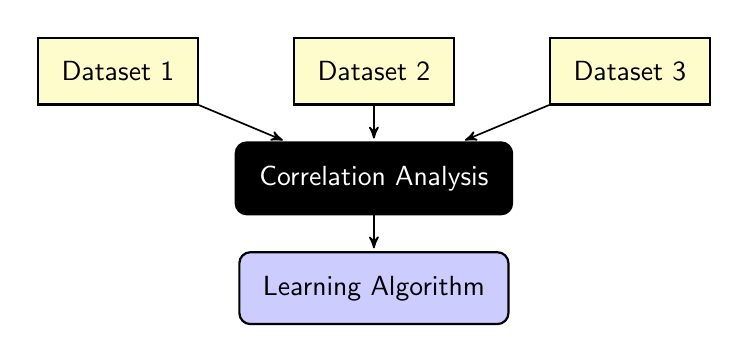
\begin{tikzpicture}[
      font=\sffamily, every matrix/.style={ampersand replacement=\&,column sep=3ex,row
      sep=3ex}, dataset/.style={draw,thick,fill=yellow!20,inner sep=.3cm},
      sink/.style={dataset,rounded corners,fill=black, text=white},
      app/.style={dataset,rounded corners,fill=blue!20}, dots/.style={gray,scale=2},
      to/.style={->,>=stealth',shorten >=1pt,semithick,font=\sffamily\footnotesize}, every
      node/.style={align=center}]

      \matrix{ \node[dataset] (dataset1) {Dataset 1}; \& \node[dataset] (dataset2)
        {Dataset 2}; \& \node[dataset] (dataset3) {Dataset 3}; \\

        \& \node[sink] (blackbox) {Correlation Analysis}; \& \\

        \& \node[app] (application) {Learning Algorithm}; \& \\ };

      \draw[to] (dataset1) -- (blackbox); \draw[to] (dataset2) -- (blackbox); \draw[to]
      (dataset3) -- (blackbox); \draw[to] (blackbox) -- (application);

    \end{tikzpicture}
    \caption{Illustration of multi-modal data fusion}
    \label{fig:data_fusion}
\end{center}
\end{figure}


\section{Canonical Correlation Analysis (CCA)}

\subsection{What is it? What is it not?}

Canonical correlation analysis (CCA) is a joint dimensionality reduction algorithm for
exactly two datasets that finds a linear transformation for each dataset such that the
correlation between the two transformed feature sets is maximized
\cite{hotelling1936relations}. CCA, however, \textit{is not} a data fusion algorithm. CCA
returns two linear transformations and a set of correlations. In this light, CCA is
extremely similar to principle component analysis (PCA), which returns a linear
transformation that accounts for the directions of largest possible variance in a
dataset. These principle components are typically used as features vectors in a variety of
machine learning algorithms. Just as PCA is a dimensionality reduction algorithm and not
the final machine learning algorithm that uses the principle components, CCA is a joint
dimensionality reduction algorithm whose dimensionality reduction ensures that datasets
are maximally correlated in their reduced spaces. These maximally correlated features may
then be used however a learning algorithm desires. 

The solution to CCA is easily found by solving a quadratic optimization problem. This
solution is a closed form expression relying on the singular value decomposition (SVD) of
a matrix product involving the covariance matrices of each dataset and the
cross-covariance between the two datasets. As these covariance matrices are rarely known
\textit{a priori}, practical uses of CCA rely on substituting sample covariance matrices
formed from training data, which we call empirical CCA.

The performance of empirical CCA has been studied previously, but insufficiently. When the
number of training samples is large compared to the dimensions of the datasets, the
performance is well understood \cite{gunderson1997estimating}. When the number of training
samples is less than the sum of the dimension of each dataset (sample deficient regime),
\cite{pezeshki2004empirical} proves that empirical CCA completely breaks down and always
reports a perfect correlation between the datasets. 

This extremely undesirable characteristic of empirical CCA has lead many to abandon CCA as
a reliable statistical analysis technique. Pezeshki, L.L. Scharf et al. argue that in this
sample deficient regime
\begin{quote}
  ... the \textcolor{red}{empirical canonical correlations are defective and
    may not be used} as     estimates of canonical correlations between random
  variables.\cite{pezeshki2004empirical}
\end{quote}
Similarly, Ge et al. conclude that
\begin{quote}
... CCA provide(s) \textcolor{red}{reliable information} about spatial
    correlations existing among pairs of data sets \textcolor{red}{only when SNRs ... are
    reasonably high, and the sample support is significantly larger than the data
    dimensions.}\cite{ge2009does}
\end{quote}



\subsection{Variations on CCA}

Due to this undesirable breakdown of CCA in the low-sample high-dimensionality regime,
many researchers proposed variations of CCA to avoid this performance loss. Most notably,
\cite{nadakuditi2011fundamental} used recent results from random matrix theory to
demonstrate that this performance breakdown may be avoided by trimming the sample
covariance matrix estimates to only include informative components. This algorithm is the
crux of this thesis. We will study its performance and develop theoretical tools in order
to use it for real-world applications. Throughout the thesis, we use the ubiquitous
low-rank signal-plus-noise model for datasets \be X = UV^H + Z, \ee where
$X=[x_1,\dots,x_n]$ is our observed data matrix whose columns are individual
multidimensional observations, $U$ is a low-rank signal subspace, $V$ is a low-rank signal
matrix, and $Z$ is a noise matrix. Surprisingly, correlation analysis for this classical
low-rank signal-plus-noise model is not completely studied. This thesis seeks to complete
the discussion. Here, we briefly touch on other variations based on CCA that do not assume
the above linear low-rank signal-plus-noise model. Many of these algorithms are tuned for
a specific application or seek to avoid the performance loss of CCA in a certain regime.

Regularized CCA (RCCA) \cite{vinod1976canonical} adds a penalty term to the magnitude of
the canonical vectors. This results in adding a scaled copy of the identity matrix to the
sample covariance matrix of each dataset, which allows each matrix to be
inverted. Therefore, RCCA returns non-trivial results in the sample-deficient
regime. However, this approach introduces a parameter to the algorithm; the effect of this
parameter is not well studied. Other variations of RCCA, such as supervised
RCCA \cite{thum2014supervised}, fast RCCA \cite{cruz2014fast}, and a multi-block RCCA
\cite{tenenhaus2014regularized}, have also been proposed.

Kernel CCA (KCCA) \cite{akaho2006kernel} was proposed to deal with non-linear correlations
existing between datasets. However, KCCA also introduces regularization parameters so as
to not return trivial solutions (see \cite{welling2005kcca} for an excellent
derivation). Besides the choice of regularization parameter, there is also ambiguity in
the choice of the kernel function, which is a common problem among kernel methods. Other
variations of KCCA have also been proposed, such as penalized KCCA
\cite{waaijenborg2009correlating}, alpha-beta divergence \cite{mandal2013non}, and CCA
based on kernel target alignment \cite{chang2013canonical}. 

Sparse CCA \cite{hardoon2011sparse} finds linear transformations such that the number of
features used is minimized. This problem is often motivated by the need for interpretable
canonical vectors that is often driven by the application, such as in brain imaging
\cite{yan2014accelerating}. There are many variations on sparse CCA, typically motivated
by application or mathematical intrigue. Sun and Keates \cite{sun2013canonical} explore
CCA in the context of censoring, Shin and Lee examine sparse functional data
\cite{shin2015canonical}, Tao et al. consider joint sparse data in
\cite{tao2014exploring}, Gao et al. explore efficient sparse CCA for high-dimensional
data \cite{gao2014efficient}, and Zhang et al. extend the analysis to multi-class group
sparse CCA \cite{zhang2013binary}. Other formulations include a penalized decomposition
\cite{witten2009penalized}, Bayesian CCA via group sparsity \cite{klami2013bayesian}, and
recursive sparse CCA \cite{chu2013sparse}.

\subsection{Applications}

CCA and its variants are widely used in a variety of fields where multiple datasets
naturally arise, the most common of which is machine learning and computer vision. In
\cite{hardoon2004canonical}, CCA is used to learn semantics of multimedia content by
fusing image and text data. Related, \cite{dhillon2011multi} uses CCA to learn word
embeddings for supervised natural language processing tasks. CCA has been widely applied
to pose estimation \cite{melzer2001nonlinear,zhai2015instance}, as this is a natural
examples where we have multiple views (image) of the same object. Other computer vision
related tasks where correlation methods are natural fits include matching people across
cameras \cite{lisanti2014matching}, clustering social event images
\cite{ahsan2014clustering}, automatic image annotation \cite{hardoon2006correlation}, and
audio-visual speaker clustering \cite{chaudhuri2009multi}.

Medical analysis is another field where there are ripe opportunities for correlation
analysis due to the vast number of modalities (EEG, MRI, CT, fMRI, MEG, etc.). CCA is
often used to determine interactions, or connectivities, between brain areas in fMRI data
\cite{deleus2011functional,arbabshirani2010comparison,khalid2013improving,guccione2013functional}
and used to fuse fMRI, sMRI, and EEG data \cite{correa2010canonical}. CCA based methods
have also been used to examine genetic connections
\cite{lin2013identifying,seoane2014canonical,lin2013group}, relying heavily on sparse
methods due to the high dimensionality of gene data and need to interpret which genes are
``on''. CCA is also a popular way to detect frequencies in steady-state visual evoked
potential (SSVEP) in brain-computer interfaces (BCIs)
\cite{zhang2013l1,nakanishi2014enhancing,zhang2014frequency}. Still further, CCA is used
in de-noising and analysis of EEG, MEG and ECG data
\cite{spuler2013spatial,campi2013non,chen2014removal,kuzilek2014comparison}.

CCA also has roots in classical signal processing applications. The authors of
\cite{via2005canonical} apply CCA to to the common communications problem of blind
equalization of single-input multiple-output (SIMO) channels. Pezeshki et al.
\cite{pezeshki2006canonical} showed that the CCA coordinates are the correct coordinates
for low-rank Gauss-Gauss detection and estimation. Scharf and Thomas
\cite{scharf1998wiener} provide a wonderful exposition on using the canonical coordinates
for Wiener filters, transform coding, filtering, and quantizing. CCA and multiset CCA have
been used to achieve joint blind source separation (BSS) in \cite{li2009joint}. CCA has
also been applied to hyperspectral imaging \cite{nielsen2002multiset}, array processing
\cite{ge2009does}, Gaussian channel capacity \cite{scharf2000canonical}, and cognitive
radio networks \cite{manco2014kernel}.

Other fun and interesting applications include climatology, finance, and music. Todros and
Hero define a new measure transformed based CCA and show its utility on financial data in
\cite{todros2012measure}. Torres et al. \cite{torres2007finding} use sparse CCA to label
portions of musical songs with meaningful words or phrases. In the field of climatology,
CCA has been used to study sea temperatures \cite{wilks2014probabilistic}, forest planning
\cite{prera2014using}, and tropical cyclones \cite{steward2014assimilating}. Finally, I
would be remiss if I didn't share my personal favorite application of CCA to date: using
CCA to analyze bovine growth \cite{li2010canonical}.

\section{Contributions of this thesis}

In many of the application presented above, researchers either have access to many
samples, or have designed an algorithm tuned specifically for a their particular
application. This thesis considers the performance of empirical correlation algorithms in
the low-sample, high dimensional setting. These algorithms are not geared toward a
particular application but are general and may be applied to any application. We will
demonstrate, both theoretically and empirically, that multi-modal correlation analysis in
this regime is a possibility. We remark that statements labeled as theorems represent, to
the best of our knowledge, new results while important results from literature are labeled
as propositions or lemmas. Chapters II-III are self contained and may be read
independently. Chapters IV-X consider the problem of correlation analysis.

Chapters \ref{sec:chpt_msd} and \ref{sec:chpt_msd_exten} consider the classical problem of
matched subspace detectors. We use insights from random matrix theory on the accuracy of
subspace estimates to derive new, optimal detectors that demonstrate the sub-optimality of
the classical plug-in detectors that simply substitute maximum likelihood estimates for
unknown parameters. Under both a stochastic and deterministic data model, we argue that
only the \textit{informative} subspace components should be used in a detector. We extend
this analysis to the case where our observations may contain missing data.

In Chapters \ref{sec:chpt_cca_det} and \ref{sec:chpt_cca_vects}, we explore the
performance of CCA and re-derive informative CCA (ICCA). We demonstrate the extreme
sub-optimality of CCA in the low-sample, high dimensionality regime. Specifically, we
provide a statistical test for both CCA and ICCA that determines whether the correlations
returned by the algorithms do indeed represent a true underlying correlation in the
datasets. We prove when each of these statistics are consistent to showcase the
superiority of ICCA. We also provide an analogous statistical test and consistency theorem
to use when the datasets have missing data entries. We create 3 new real-world,
multi-modal datasets involving video and audio to verify the performance of ICCA. We then
showcase that the canonical vectors returned by ICCA are more accurate than the CCA
vectors in the low-sample regime. Finally, we provide a new algorithm for estimating the
canonical vectors that asymptotically optimal.

Next, we explore the performance of regularized CCA (RCCA) in Chapter
\ref{sec:chpt_rcca}. When the number of training samples is limited but correlation
analysis is still desired, a common strategy is to regularize CCA by adding a penalty to
the magnitude of the linear transformation. However, we demonstrate that setting the
regularization parameter to infinity results in the best performance. In fact, in this
setting, the solution to RCCA may be found by taking the SVD of the sample
cross-covariance matrix between the two datasets. We then predict the behavior of the
largest singular values of this cross-covariance matrix assuming a low-rank
signal-plus-noise model on the individual datasets. We argue that using the top singular
values of this cross-covariance matrix to detect correlations is sub-optimal because the
correlation coefficients are coupled with the individual data signal strengths.

Using a similar proof technique, we predict the behavior of the largest singular values of
the projection of low-rank signal plus noise matrices to a smaller dimension in Chapter
\ref{sec:chpt_svd_proj}. Specifically, we consider two types of projection matrices: one
with standard complex Gaussian entries and one with orthonormal columns. We are able to
provide a closed form expression for the largest singular values in the case where the
projection matrix is unitary. Through numerical simulations, we demonstrate the
superiority of the unitary projection matrix over the Gaussian projection matrix. The
unitary projection matrix can reliably detect the signals at a lower signal-to-noise ratio
than the Gaussian projection matrix. 

In Chapter \ref{sec:chpt_det_reg} we apply CCA and ICCA to the classical problems of
detection and regression. First, we consider the low-rank signal-versus-noise subspace
detection problem given two datasets. We prove that the standard likelihood ratio test
(LRT) detector may be written using the canonical basis returned by CCA. We show that when
using empirical parameter estimates, the CCA detector is extremely suboptimal but that the
ICCA detector is equivalent to the plug-in LRT detector. We then show that the classical
Gaussian regression problem may be written in terms of the CCA basis. However, similar to
the detection problem, empirical CCA degrades the performance significantly while ICCA
matches the classical plug-in detector. We show this via mean squared error prediction
plots.

We then consider the joint problems of image retrieval and image annotation in Chapter
\ref{sec:chpt_ia}. Correlation based methods are typically overlooked as solutions to such
problems due to the problems with CCA outlined in this thesis. We show that using ICCA to
solve these problems results in non-trivial solutions. We compare the performance of CCA
and ICCA on four different image-text datasets and describe the capabilities and
limitations of ICCA in this application. When the datasets contain multiple images of the
same objects and meaningful captions, ICCA is able to capture correlations between images
and text. However, ICCA fails to capture semantic meanings between documents and
captions. We argue that with clever feature engineering and improved NLP techniques,
correlation based methods may be relevant for image retrieval and image annotation.

Lastly, we consider multi-set CCA (MCCA) in Chapter \ref{sec:chpt_mcca}. Unfortunately,
unlike CCA, there is no clear objective function to use in an optimization problem;
Kettenring \cite{kettenring1971canonical} proposes five such objective functions. Nielsen
also provides a nice formulation of MCCA in \cite{nielsen1994analysis} where he proposes
four constraint functions.  We provide derivations for these 20 formulations, in both a
theoretical and empirical setting. We then choose to consider the MAXVAR problem as we are
able to directly apply our insights from ICCA to create an informative version of it,
which we call informative MCCA (IMCCA). We demonstrate the superior performance of IMCCA
on a real-world video dataset that we created. 


\section{Data Model and Background}\label{sec:chpt6:data_model}
\subsection{Training Data Model}\label{sec:training_data}We are given
  $m$ signal-bearing training vectors $y_i\in \complex^{n\times 1}$, $i=1,\dots,m$, modeled\footnote{For expositional simplicity, we have assumed that all our matrices and vectors are complex-valued; our results also hold for real-valued matrices and vectors.} as $y_i=Ux_i+z_i$ where $z_i\overset{\text{i.i.d.}}{\sim}\mathcal{CN}(0,I_n)$, $U$ is an unknown $n\times k$ complex matrix with orthonormal columns, and $x_i\overset{\text{i.i.d.}}{\sim}\mathcal{CN}(0,\Sigma)$ where $\Sigma=\diag(\sigma_1^2,\dots,\sigma_k^2)$ with $\sigma_1>\sigma_2>\dots>\sigma_k>0$ unknown. For each observation, $x_i$ and $z_i$ are independent. The dimension, $k$, of our subspace is unknown and we assume throughout that $k\ll n$ so that we have a low-rank signal embedded in a high-dimensional observation vector.

  Given a dimension estimate, $\widehat{k}$, and the signal bearing training data $Y = \begin{bmatrix} y_1 & \dots & y_m \end{bmatrix}$, we form a subspace estimate $\widehat{U}\in\complex^{n\times\widehat{k}}$ by taking the leading $\widehat{k}$ eigenvectors of $YY^{H}/m$ and a signal covariance estimate $\widehat{\Sigma}\in\reals^{\widehat{k}\times\widehat{k}}$ (in a manner to be specified).

\subsection{Testing Data Model}
We will consider two models for the test vectors. In the stochastic setting, the test vector $y\in\complex^{n\times 1}$ is modeled as
\begin{equation}\label{eq:stoch_setup}
\text{Stochastic Model: }y=\left\{
\begin{aligned}
&z
&& y\in H_0:\text{ Noise only}\\
&Ux+z
&& y\in H_1:\text{ Signal-plus noise}\\
\end{aligned}\right. ,
\end{equation}
where $U$, $z$, and $x$ are modeled as described in Section \ref{sec:training_data}. This assumes that the signal, $Ux$, may lie anywhere in the subspace and whose position in the subspace is governed by the signal covariance matrix $\Sigma$.

In the deterministic setting, the test vector $y\in\complex^{n\times 1}$ is modeled as
\begin{equation}\label{eq:determ_setup}
\text{Deterministic Model: }y=\left\{
\begin{aligned}
&z
&& y\in H_0:\text{ Noise only}\\
&U\Sigma^{1/2} x+z
&& y\in H_1:\text{ Signal-plus noise}\\
\end{aligned}\right. ,
\end{equation}
where $U$, $\Sigma$, and $z$ are modeled as before. Here, in contrast to the stochastic setting, $x$ is a non-random deterministic vector. Thus the signal, $U\Sigma^{1/2}x$, lies at a fixed point in the unknown subspace. Note that placing a mean zero, identity covariance Gaussian prior on $x$ in (\ref{eq:determ_setup}) yields the stochastic model described in (\ref{eq:stoch_setup}).

\subsection{Problem 1: Characterize the ROC Performance Curves}\label{sec:problem 1}
Given an independent test observation from (\ref{eq:stoch_setup}) or (\ref{eq:determ_setup}), we first use $\widehat{U}$ to generate a $\widehat{k}\times 1$ test vector $w=\widehat{U}^Hy$. The vector $w$ is a sufficient statistic \cite{scharf1991statistical} when $\widehat{U} = U$. We focus on detectors of the form
\begin{equation}\label{eq:detector_form}
w^HDw\detgtrless\eta,
\end{equation}
where $D$ is a diagonal matrix and the test statistic $\Lambda(w) := w^HDw$ is compared against a threshold, $\eta$, set to achieve a prescribed false alarm rate $\alpha$. For detectors of this form and for test vectors modeled as (\ref{eq:stoch_setup}) or (\ref{eq:determ_setup}), our goal is to
\begin{center}
Predict $P_D=:\mathbb{P}(\text{Detection})$, for every $P_F:=\alpha \in (0,1)$ given $n$, $m$, $\widehat{k}$, $D$ and $\Sigma$.
\end{center}

This performance prediction relies on RMT results quantifying the accuracy of the subspace estimate $\widehat{U}$ as a function of the parameters listed.
%We will consider detectors, $g(w)\to\{H_0,H_1\}$, which solve
%\begin{equation}\label{eq:maximization}
%\begin{aligned}
%&\text{maximize}
%&& P_D=P\left(g(w)\to H_1 | w\in H_1\right)\\
%&\text{subject to}
%&& P_F=P\left(g(w)\to H_1 | w\in H_0\right)\leq\alpha\\
%\end{aligned}
%\end{equation}
%where $\alpha\in[0,1]$.

\subsection{Problem 2: Derive and Predict the Performance of a Detector that Exploits  Predictions of Subspace Accuracy}\label{sec:ps_prob2}
In the  Neyman-Pearson setting (see \cite{van1968detection}), a MSD is a likelihood ratio test (LRT) taking the form
\begin{equation*}
\Lambda(w):=\dfrac{f(w|H_1)}{f(w|H_0)} \detgtrless \eta
\end{equation*}
where $\Lambda(w)$ is the test statistic, $\eta$ is the threshold set to achieve a given false alarm rate, and $w = \widehat{U}^{H}y$. Here, $\widehat{U}$ is a noisy estimate of the underlying $U$; its accuracy, relative to $U$, can be quantified using RMT. Therefore, $f(w|H_0)$ and $f(w|H_1)$, and consequently $\Lambda(w)$, depend on the `noisiness' of the estimated subspaces.  Our goal is thus to
\begin{quote}
Design \& analyze the performance of  a detector that exploits RMT predictions of subspace estimation accuracy.
\end{quote}
The design and performance prediction aspect of this problem will provide insights on when, if, and how the performance of plug-in detectors that do not exploit the knowledge of subspace estimation accuracy can be improved.


%and we employ the generalized likelihood ratio test (GLRT). It is standard to substitute estimates $\widehat{U}$  and $\widehat{\Sigma}$ for the unknown $U$ and $\Sigma$ in the oracle test statistic \cite{jin2005cfar,mcwhorter2003matched}. This resulting plug-in detector assumes that the parameter estimates are exact. Through our analysis, we characterize the performance loss associated with making this assumption and derive a new detector which can systematically avoid this performance loss. By relying on the subspace accuracy estimates presented in Theorem \ref{th:angles}, the new RMT detector only utilizes $\min(\widehat{k},k_\text{eff})$ subspace components to form an approximation to the oracle detector. In both testing scenarios, the plug-in and RMT detectors take the desired form of (\ref{eq:detector_form}).


\section{Main Results}\label{sec:chpt6:main_results}
Figure \ref{fig:chpt6:rcca} shows the empirical performance of RCCA for various
regularization parameters. Evident in this figure, we observe that increasing the
regularization parameter increases the performance of RCCA. The following theorem gives
the solution of RCCA when taking $\eta\to\infty$. 

\begin{Th}\label{thm:lrcca}
Let $\widetilde{X}_n$ and $\widetilde{Y}_n$ be modeled as in (\ref{eq:model}). Let
$\Clrcca=\frac{1}{n}\widetilde{X}_n\widetilde{Y}_n^T$ have SVD $FKG^T$ where $F=[f_1,\dots,f_{p}]$,
  $K=\diag(k_1,\dots,k_{\min\left(p,q\right)})$, and $G=[g_1,\dots,g_{q}]$. When $\eta\to\infty$, the solution to
the RCCA optimization problem in (\ref{eq:rcca_opt}) is 
\beq\label{eq:lrcca}\ba
&\rho \propto k_1\\
&\xI \propto f_1\\
&\xII \propto g_1.\\
\ea\eeq
\end{Th}
\begin{proof}
See Section \ref{sec:lrcca_proof}.
\end{proof}

We call the above algorithm limit RCCA (LRCCA), which is preferred over RCCA as it both
offers better performance and has no tuning parameter. Next we characterize the asymptotic
limit of the top singular values of $\Clrcca$. 

\begin{Th}\label{thm:xy_sv}
Let $\widetilde{X}_n$ and $\widetilde{Y}_n$ be modeled as in (\ref{eq:model}) and define
$C_n=\frac{1}{n}\widetilde{X}_n\widetilde{Y}_n^T$. Let $p\to\infty$, $q\to\infty$, and $n\to\infty$
such that $\frac{p}{n}\to c_x$ and $\frac{q}{n}\to c_y$. Given the noise matrices $X_n$
and $Y_n$, define $R_n=\frac{1}{n}X_n^TX_n$ and $S_n=\frac{1}{n}Y_n^TY_n$. Let $\mu_{R_n}$
and $\mu_{S_n}$ be the respective empirical eigenvalue distributions and assume that each
converges almost surely weakly, 
as $n,p,q\to\infty$ as above, to the non-random compactly supported probability measures
$\mu_R$ and $\mu_S$, respectively. Similarly, let $M_1=\frac{1}{n^2}X_nY_n^TY_nX_n^T$,
$M_2=\frac{1}{n^2}Y_nX_n^TX_nY_n^T$, and $M_3 = M_1\left(\sigma_i^2-M_1\right)^{-1}$ have
limiting eigenvalue distributions $\mu_{M_1}$, $\mu_{M_2}$, and $\mu_{M_3}$
respectively. For $i=1,\dots,r$, let $\sigma_i$ be the larest singular values of $C_n$.
Then, almost surely, $\sigma_i$ are the solutions to the following equation
\beq\label{eq:thm}
 0=\prod_{i=1}^r\left(\varphi_H(\sigma_i)\varphi_F(\sigma_i) -
\frac{1}{\theta_{yi}^2}\right)\left(\varphi_J(\sigma_i)\varphi_G(\sigma_i) -
\frac{1}{\theta_{xi}^2}\right) -
\rho_i^2\varphi_H(\sigma_i)\varphi_G(\sigma_i)\left(1+\varphi_K(\sigma_i)\right)^2
\eeq
where 
\be\ba
& \varphi_F(\sigma_i) = -\sigma_i\E{xm_{\mu_{RS|R}}\left(\sigma_i^2,x\right)}_{\mu_R}\\
& \varphi_J(\sigma_i) = -\sigma_i\E{xm_{\mu_{RS|S}}\left(\sigma_i^2,x\right)}_{\mu_S}\\
& \varphi_G(\sigma_i) = -\sigma_im_{\mu_{M_1}}(\sigma_i^2) \\
& \varphi_H(\sigma_i) = -\sigma_im_{\mu_{M_2}}(\sigma_i^2) \\
& \varphi_K(\sigma_i) = c_x\E{x}_{\mu_{M_3}}\\
\ea\ee
and
\be
m_{\mu_M}(z) = \int \frac{1}{t-z}d\mu_M(t)
\ee
is the Stieltjes transform of $\mu_M$ and
\be
m_{\mu_{XY|X}}(x,y) = \int \frac{1}{y-z}k_{XY|X}(x,z)dz
\ee
where $k_{XY|X}$ is the Markov transition kernel density function. 
\end{Th}
\begin{proof}
See Section \ref{sec:xy_sv_proof}.
\end{proof}


\section{Empirical Simulations}\label{sec:chpt6:emp_results}
In this section we first motivate the need for LRCCA by exploring the performance of RCCA
for various regularization parameters. We then explore the accuracy of Theorem
\ref{thm:xy_sv}. While this theorem gives an asymptotic limit, we show that the
finite-sized approximation holds for moderately sized systems. 

For all of the following simulations, we generate correlated signal datasets by
\be\ba
&\widetilde{X}^{\text{signal}} = \left[\widetilde{x}_1^{\text{signal}},\dots,\widetilde{x}_n^{\text{signal}}\right]\\
&\widetilde{Y}^{\text{signal}} = \left[\widetilde{x}_1^{\text{signal}},\dots,\widetilde{y}_n^{\text{signal}}\right]
\ea\ee
where
\be\ba
&\widetilde{x}_i^{\text{signal}} = U_x\Theta_xv_x^{(i)} + x_i\\
&\widetilde{y}_i^{\text{signal}} = U_y\Theta_yv_y^{(i)} + y_i,
\ea\ee
where $x_i\sim\mathcal{N}(0,I_p)$ and $y_i\sim\mathcal{N}(0,I_q)$ and
\be 
\left[\begin{array}{c}v_x^{(i)}\\v_y^{(i)}\end{array}\right]
\sim\mathcal{N}\left(\left[\begin{array}{cc}I_r &P\\P^T &I_r \end{array}\right]\right).
\ee
$P=\diag(\rho_1,\dots,\rho_r)$ with $0\leq\rho_i\leq1$ and
$\Theta_x=\diag(\theta_{x1},\dots,\theta_{xr})$ and
$\Theta_y=\diag(\theta_{y1},\dots,\theta_{yr})$ with $\theta_{xi}\geq0$ and
$\theta_{yi}\geq0$. We generate $U_x$ by taking the eigenvectors corresponding to the top
$r$ eigenvalues of a random $p\times p$ matrix with $\mathcal{N}(0,1)$ entries. We
generate $U_y$ independently in a similar manner. 

We then generate noise only datasets
\be\ba
&\widetilde{X}^{\text{noise}} =
\left[\widetilde{x}_1^{\text{noise}},\dots,\widetilde{x}_n^{\text{noise}}\right]\\ 
&\widetilde{Y}^{\text{noise}} =
\left[\widetilde{x}_1^{\text{noise}},\dots,\widetilde{y}_n^{\text{noise}}\right] 
\ea\ee
where
\be\ba
&\widetilde{x}_i^{\text{noise}} \sim\mathcal{N}(0,I_p)\\
&\widetilde{y}_i^{\text{noise}} \sim\mathcal{N}(0,I_q).
\ea\ee

\subsection{Performance of RCCA}

First we explore the effect of the regularization parameter in RCCA. For the above simulation
setup we generate both correlated signal data matrices and
with $r=1$ and noise only data matrices. We are interested the distribution of the
correlation estimate, $\widehat{\rho}$, returned by RCCA when there is a correlation present
($\widetilde{X}^{\text{signal}}$ and $\widetilde{Y}^{\text{signal}}$), and when there is no
correlation present ($\widetilde{X}^{\text{noise}}$ and
$\widetilde{Y}^{\text{noise}}$). 

For a fixed $p=100$, $q=150$, and $\rho_1=0.9$ we compute this RCCA correlation estimate
under each hypothesis for 500 trials giving
$\left[\widehat{\rho}_1^{\text{signal}},\dots,\widehat{\rho}_{500}^{\text{signal}}\right]$
and
$\left[\widehat{\rho}_1^{\text{noise}},\dots,\widehat{\rho}_{500}^{\text{noise}}\right]$. We
then compute the empirical ROC (receiver operating characteristic) curve for these two
statistics and the resulting AUC (area under the ROC curve). We repeat this process by
varying $\theta=\theta_{x1}=\theta_{y1}$ and $n$. We plot AUC heatmaps for four different
values of the RCCA regularization parameter in Figure \ref{fig:chpt6:rcca}. AUC values close to
0.5 indicate the distributions of $\widehat{\rho}^{\text{signal}}$ and
$\widehat{\rho}^{\text{noise}}$ are not separable while values close to 1 indicate that
they are perfectly separable. 

As evident in this figure, the ability of RCCA to detect the presence of a signal increases
with the regularization parameter. This is a non-intuitive result as typical regularized
algorithms` have an optimal regularization parameter that maximizes performance. The
non-monotonicity of the AUC heatmaps evident in Figures \ref{fig:chpt6:rcca1} and
\ref{fig:chpt6:rcca2} also give credence to the difficulty in selecting an appropriate
regularization parameter. In certain regimes, increasing the number of samples reduces
performance, which is a very undesirable property. Based on these empirical observations
about the effect of the regularization parameter in RCCA, we conclude that setting
$\eta\to\infty$ results in optimal performance of RCCA. As is stated in Theorem
\ref{thm:lrcca}, in this regime the solution RCCA is found by simply taking the SVD of
$\frac{1}{n}\widetilde{X}\widetilde{Y}^T$. 

\begin{figure}[h!]
  \centering
  \subfigure[$\eta=0.0001$]{
    \label{fig:chpt6:rcca1}
    \includegraphics[width=0.4\textwidth]{chpt6_xy/figures/eta1_auc.pdf}
  }
  \subfigure[$\eta=0.1$]{
    \label{fig:chpt6:rcca2}
    \includegraphics[width=0.4\textwidth]{chpt6_xy/figures/eta2_auc.pdf}
  }
  \subfigure[$\eta=10$]{
    \label{fig:chpt6:rcca3}
   \includegraphics[width=0.4\textwidth]{chpt6_xy/figures/eta3_auc.pdf}
  }
  \subfigure[$\eta=1000$]{
    \label{fig:chpt6:rcca4}
    \includegraphics[width=0.4\textwidth]{chpt6_xy/figures/eta4_auc.pdf}
  }
  \caption{AUC performance of RCCA for various regularization parameters. For all figures, $p=100$,
    $q=150$, $r=1$, and $\rho_1=0.9$. Each figure plots an AUC heatmap while sweeping over
  $\theta=\theta_{x1}=\theta_{y1}$ and $n$. AUC points are generated from an ROC formed
  from 500 points of each distribution. Increasing the regularization parameter increases
  the performance of CCA. This gives rise to LRCCA, which sets $\eta\to\infty$.}
  \label{fig:chpt6:rcca}
\end{figure}

\subsection{Numerical Accuracy of Theorem \ref{thm:xy_sv}}

For $p=200$, $q=400$, $n=400$, and $\rho=1$ we compute the largest singular value returned
by LRCCA for various $\theta=\theta_{x1}=\theta_{y1}$. This is repeated and for 100 trials
and compared to the theoretical prediction. Results are shown in Figure \ref{fig:chpt6:sv_pred}
and confirm the accuracy of our theoretical prediction. As evident in Figure
\ref{fig:chpt6:sv_pred}, if $\theta$ is below a critical value, the largest singular value does
not change and remains constant. This phase transition phenomenon arises in similar
analyses of eigenvalue decomposition and SVDs of signal-plus-noise models \cite{benaych2011eigenvalues,benaych2012singular,paul2007asymptotics}. This limiting value is the largest singular value of the noise matrix
$\frac{1}{n}XY^T$, which we define as $b=\sigma_1\left(XY^T\right)$. Substituting $b$ into
(\ref{eq:thm}) we have the following equality
\beq\label{eq:pt}
 0=\left(\varphi_H(b)\varphi_F(b) -
\frac{1}{\theta_{y1}^2}\right)\left(\varphi_J(b)\varphi_G(b) -
\frac{1}{\theta_{x1}^2}\right) -
\rho\varphi_H(b)\varphi_G(b)\left(1+\varphi_K(b)\right)^2.
\eeq
This equation may be solved for any desired parameter $c_x, c_y, \theta_{x1}, \theta_{y1},
\rho$, while keeping the rest fixed. We note that the $\varphi$ functions and $b$ are implicitly dependent on $c_x$ and $c_y$.

\begin{figure}
  \begin{center}
    \includegraphics[width=0.6\textwidth]{chpt6_xy/figures/sigma_pred.pdf}
    \caption{Top singular value prediction for the rank-1 case for $p=200$, $q=400$,
      $n=400$, and $\rho=1$.}
    \label{fig:chpt6:sv_pred}
  \end{center}
\end{figure}

Figure \ref{fig:chpt6:lrcca_pt} plots the top singular value returned by LRCCA when the datasets
contain $r=1$ signal each, empirically averaged over 500 trials. Each heatmap sweeps over
two parameters while keeping the rest constant. We then solve (\ref{eq:pt}) by
substituting our constant parameters to achieve a function of the two parameters that we
sweep. We overlay this line in each heatmap. Below this line the
top singular value is indistinguishable from that returned by LRCCA with noise only
datasets.

\begin{figure}[!htbp]
  \centering
  \subfigure[$\rho=1$, $\theta=\theta_{x1}=\theta_{y1}$]{
    \label{fig:chpt6:rcca1}
    \includegraphics[width=0.4\textwidth]{chpt6_xy/figures/n_theta_large.pdf}
  }
  \subfigure[$\rho=0.1$, $\theta=\theta_{x1}=\theta_{y1}$]{
    \label{fig:chpt6:rcca2}
    \includegraphics[width=0.4\textwidth]{chpt6_xy/figures/n_theta_small.pdf}
  }
  \subfigure[$\theta_{x1}=\theta_{y1}=1$]{
   \includegraphics[width=0.4\textwidth]{chpt6_xy/figures/n_rho.pdf}
  }
  \subfigure[$n=400$]{
    \includegraphics[width=0.4\textwidth]{chpt6_xy/figures/rho_theta.pdf}
  }
  \subfigure[$\rho=0.5$, $n=400$]{
    \includegraphics[width=0.4\textwidth]{chpt6_xy/figures/theta_theta.pdf}
    \label{fig:chpt6:theta_theta}
  }
  \caption{Top singular value of LRCCA plotted for pairs of parameter sweeps. In all
    plots, $p=200$ and $q=400$. The theoretical boundary where the top singular value is
    indistinguishable from a noise only setting is plotted for each. Below this line, the
    top singular value is asymptotically identical to the noise only setting. Above this
    line, the top singular value is asymptotically different from that of the noise only
    setting.}
  \label{fig:chpt6:lrcca_pt}
\end{figure}

Next we explore the phase transition in Figure \ref{fig:chpt6:theta_theta} for a fixed $n=400$
and numerous $\rho$. Instead of plotting the top singular value returned by LRCCA, we
instead plot the log of the KS-statistic between the singular values in the signal bearing case
and the singular values in the noise bearing case. A KS statistic of 1 represents
perfectly distinct distributions while a KS statistic of 0 represents the same
distribution. We plot the results in Figure \ref{fig:chpt6:lrcca_ks} and it is evident
that our theoretical phase transition in (\ref{eq:pt}), which relies on Theorem
\ref{thm:xy_sv}, is very accurate even though we apply the asymptotic result to the finite
dimensional setting.  

\begin{figure}[!htbp]
  \centering
  \subfigure[$\rho=1$]{
    \label{fig:chpt6:rcca1}
    \includegraphics[width=0.4\textwidth]{chpt6_xy/figures/rho_10_theta.pdf}
  }
  \subfigure[$\rho=0.8$]{
    \label{fig:chpt6:rcca2}
    \includegraphics[width=0.4\textwidth]{chpt6_xy/figures/rho_8_theta.pdf}
  }
  \subfigure[$\rho=0.6$]{
   \includegraphics[width=0.4\textwidth]{chpt6_xy/figures/rho_6_theta.pdf}
  }
  \subfigure[$\rho=0.4$]{
    \includegraphics[width=0.4\textwidth]{chpt6_xy/figures/rho_4_theta.pdf}
  }
  \subfigure[$\rho=0.2$]{
    \includegraphics[width=0.4\textwidth]{chpt6_xy/figures/rho_2_theta.pdf}   
  }
  \subfigure[$\rho=0$]{
    \includegraphics[width=0.4\textwidth]{chpt6_xy/figures/rho_0_theta.pdf}   
  }
  \caption{KS statistic between the top singular value of LRCCA in signal bearing and
    noise only settings. In all plots, $p=200$, $q=400$, and $n=400$. The theoretical boundary where
    the top singular value is indistinguishable from a noise only setting is plotted for
    each.}
  \label{fig:chpt6:lrcca_ks}
\end{figure}

\subsection{Comparison to ICCA}

We now compare the performance of LRCCA to that of ICCA. As shown in
\cite{nadakuditi2011fundamental} and presented in Theorem \ref{th:khat_lims}, the
correlation coefficient does not affect the performance of ICCA. The consistency phase
transition of ICCA for the rank-1 setting is  
\be
\theta_x > c_x^{1/4} \text{ and } \theta_y > c_y^{1/4}.
\ee
We plot this phase transition against the phase transitions of LRCCA for a variety of
$\rho$ in Figure \ref{fig:chpt6:icca_comp}. 

We begin our discussion by comparing what these phase transition boundaries represent for
each algorithm. The ICCA phase transition boundary represents when we reliably detect the
presence of a correlated signal. Above this boundary, the largest singular value of
$\widetilde{C}$ used in ICCA is used to statistically detect the presence of a correlated
signal. We direct the reader to Chapter \ref{sec:chpt_cca_det} for a discussion of this
process. However, if either SNR drops below its individual phase transition, ICCA is not
able to detect a correlated signal. The LRCCA phase transition boundaries, on the other
hand, represent when the largest singular value of $\Clrcca$ represents a signal, not
necessarily a correlated signal. As we saw in Figure \ref{fig:chpt6:motiv_3}, even
uncorrelated datasets will cause the largest singular value to separate from the rest of
the singular value. Therefore, these phase transition boundaries represent different
boundaries. 

One may incorrectly conclude from Figure \ref{fig:chpt6:icca_comp} that for LRCCA is
superior to ICCA since the boundary of LRCCA includes the regime when $\theta_x$ is very
small but $\theta_y$ is large, and vice versa. However, this singular value only indicates
the presence of a signal, not that it is correlated. We saw in Figure
\ref{fig:chpt6:motiv} that different values of $\theta_x,\theta_y,\rho$ can result in the
same largest singular value. Thus, simply using the largest singular value of
$\frac{1}{n}XY^H$ to determine whether correlation exists between the dataset is
incorrect. As Figure \ref{fig:chpt6:motiv_3} shows, the cross covariance matrix will have
a large singular value even if the individual datasets are independent. 

One may then want to use the relative individual SNRs of $X$ and $Y$ to determine whether
this leading singular value is large because of correlation or individual large
SNRs. However, this process of pre-whitening the data matrices $X$ and $Y$ is exactly the
process used in CCA and ICCA. Therefore, to use the cross-covariance matrix $XY^H$ to
detect the presence of correlation between the datasets, one would perform the equivalent
analysis as CCA, which is suboptimal to ICCA. Therefore, we urge users to reconsider using
the cross covariance matrix to screen for correlation and instead use ICCA.

\begin{figure}[!h]
  \begin{center}
    \includegraphics[width=0.6\textwidth]{chpt6_xy/figures/theta_theta_icca.pdf}
    \caption{Phase transition for LRCCA (dahsed lines) for various $\rho$ and ICCA. The
      performance of ICCA is independent of $\rho$. The setting shown in for $c_x=0.5$ and
    $c_y=1$. }
    \label{fig:chpt6:icca_comp}
  \end{center}
\end{figure}



\section{Proofs of Theorems \ref{thm:lrcca} and \ref{thm:xy_sv}}\label{sec:chpt6:proofs}
\subsection{Proof of Theorem \ref{thm:lrcca}}\label{sec:lrcca_proof}
We begin with the RCCA matrix $\Creg = \left(\Rxx+\eta
  I_{p}\right)^{-1/2}\Rxy\left(\Ryy +\eta I_{q}\right)^{-1/2}$. Recall the data SVDs
$\widetilde{X}=F_xK_xG_x^H$ and $\widetilde{Y}=F_yK_yG_y^H$. Substituting these into
$\Creg$ yields
\be\ba
&\Creg &&= \left(F_xK_xK_x^HF_x^H + \eta
  I_p\right)^{-1/2}F_xK_xG_x^HG_yK_y^HF_y^H\left(F_yK_yK_y^HF_y^H + \eta
  I_q)\right)^{-1/2}\\
&&& = F_x\left(K_xK_x^H + \eta I_p\right)^{-1/2}K_xG_x^HG_yK_y^H\left(K_yK_y^H + \eta I_q\right)^{-1/2}
\ea\ee

Define
$\widetilde{F}_x = F_x(:,1:\min(p,n))$, $\widetilde{F}_y = F_y(:,1:\min(q,n))$,
$\widetilde{G}_x = G_x(:,1:\min(p,n))$, and $\widetilde{G}_y =
G_y:,1:\min(q,n))$. Then 
\begin{equation}
  \Creghat = \widetilde{F}_x\diag\left(\frac{k_{xi}}{\sqrt{k_{xi}^2 +
        \eta}}\right)\widetilde{G}_x^H\widetilde{G}_y
  \diag\left(\frac{k_{yi}}{\sqrt{k_{yi}^2 +\eta}}\right)\widetilde{F}_y^H. 
\end{equation}
Clearly, as $\eta\to\infty$, this matrix becomes the zero matrix. However, the ratio of
the diagonal entries as $\eta\to\infty$ dictates the limiting form of $\Creg$. Examining
this ratio of adjacent diagonal elements yields 
\begin{equation*}
\lim_{\eta\to\infty} \frac{\sqrt{\frac{k_{xi}^2}{\sigma_{xi}^2 +
      \eta}}}{\sqrt{\frac{k_{x(i+1)}^2}{k_{x(i+1)}^2 + \eta}}} =
\lim_{\eta\to\infty}
\sqrt{\frac{k_{xi}^2\left(k_{x(i+1)}^2+\eta\right)}{k_{x(i+1)}^2\left(k_{xi}^2 +
  \eta\right)} } = \frac{k_{xi}}{k_{x(i+1)}}
\end{equation*}
Thus, as $\eta\to\infty$, the ratio of entries along the diagonal matrix approaches the
ratio between the singular values. Therefore, 
\be
\lim_{\eta\to\infty} \diag\left(\frac{k_{xi}}{\sqrt{k_{xi}^2 +
        \eta}}\right) \propto \left(K_xK_x^H\right)^{1/2}.
\ee
A similar analysis yields an analogous results for the diagonal matrix of the singular
values of $\widetilde{Y}$. Therefore, 
\begin{equation*}
  \lim_{\eta\to\infty}\Creghat \propto
  \widetilde{F}_x\left(K_xK_x^H\right)^{1/2}\widetilde{G}_x^H\widetilde{G}_y\left(K_yK_y^H\right)^{1/2}\widetilde{F}_y^H
  = \widetilde{X}\widetilde{Y}^H.
\end{equation*}
Therefore, as $\eta\to\infty$, the largest singular value of $\Creghat$ is proportional to
the largest singular value of $\frac{1}{n}\widetilde{X}\widetilde{Y}^H$. 

To complete the proof, we must show that the canonical vectors are proportional to the
singular vectors of $\frac{1}{n}\widetilde{X}\widetilde{Y}^H$. The top
canonical vector for dataset $X$ returned by RCCA is $w_x = \left(\Rxx+\eta
  I_d\right)^{-1/2}f_1$, where $f_1$ is the top left singular vector of $\Creghat$. As
$\eta\to\infty$, $\left(\Rxx+\eta I_d\right)^{-1/2}\to \frac{1}{\sqrt{\eta}}I_d$. Therefore,
$\xI\propto f_1$. Similarly, $\xII\propto g_1$. Therefore, when $\eta\to\infty$, the
solution to RCCA is
\be\ba
& \rho \propto k_1\\
& \xI \propto f_1\\
& \xII \propto g_1,\\
\ea\ee
where $k_1$ is the top singular value of $\frac{1}{n}\widetilde{X}\widetilde{Y}^H$ with
corresponding left and right singular vectors $f_1$ and $g_1$. Successive canonical
correlation and vector pairs are found via successive singular value-vector pairs.

\subsection{Proof of Theorem \ref{thm:xy_sv}}\label{sec:xy_sv_proof}

We remove the scaling $\frac{1}{n}$ for proof simplicity as this only scales the singular
value. The singular values of $\Clrcca=\widetilde{X}\widetilde{Y}^H$ are the positive eigenvalues of
\be\ba
&C_n &&= \left[\begin{array}{cc} 0 &\widetilde{X}_n\widetilde{Y}_n^H\\
\widetilde{Y}_n\widetilde{X}_n^H & 0 \end{array}\right] \\
&&&= 
\left[\begin{array}{cc} 0 & \left(U_x\Theta_xV_x^H+X_n\right)\left(U_y\Theta_yV_y^H + Y_n\right)^H\\
\left(U_y\Theta_yV_y^H + Y_n\right)\left(U_x\Theta_xV_x^H+X_n\right)^H &
0 \end{array}\right]\\
&&& = \left[\begin{array}{cc}0 & X_nY_n^H \\ YX^H & 0\end{array}\right] + U_n\Lambda U_n^H,
\ea\ee
where
\be
U_n=\left[\begin{array}{cccc}U_x &X_nV_y& 0 & 0\\ 0 & 0 & Y_nV_x+U_y\Theta_yP &U_y \end{array}\right],\,\,
\Lambda = \left[\begin{array}{cccc}0 & 0 & \Theta_x & 0 \\ 0 & 0 & 0 &\Theta_y\\
\Theta_x & 0 & 0 & 0\\ 0 & \Theta_y & 0 & 0\end{array}\right].
\ee
If $\sigma$ is an eigenvalue of $C_n$, it must satisfy
$\det\left(\sigma I_{p+q}-C_n\right)=0$. Using our expression above, this is
\beq\label{eq:det1}
\det\left(\sigma I_{p+q} - \left[\begin{array}{cc}0 & X_nY_n^H \\ Y_nX_n^H & 0\end{array}\right] -
  U_n\Lambda U_n^H\right) = 0.
\eeq
Define
\be
B_n = \left(\sigma I_{p+q} - \left[\begin{array}{cc}0 & X_nY_n^H\\ Y_nX_n^H & 0\end{array}\right]\right).
\ee
Using properties of determinants, we may re-write (\ref{eq:det1}) as
\be\ba
&\det\left(B_n -U_n\Lambda U_n^H\right) &&=
\det\left(\Lambda\right)\det\left(\Lambda^{-1}\right)\det\left(B -  U_n\Lambda U_n^H\right)\\
&&& = \det(\Lambda)\det\left(\left[\begin{array}{cc}\Lambda^{-1} & U_n^H \\ U_n &
      B_n \end{array}\right]\right)\\
&&& = \det\left(B_n\right)\det(\Lambda)\det\left(\Lambda^{-1}-U_n^HB_n^{-1}U_n\right).
\ea\ee

If $\sigma>0$ is an eigenvalue of $C_n$, it is not a singular value of $X_nY_n^H$ as by
assumption $\Lambda\neq0$. Therefore, $B_n$
is not singular and its inverse exists and it has a nonzero determinant. Therefore for
(\ref{eq:det1}) to hold,
\beq\label{eq:det2}
\det\left(\Lambda^{-1}-U_n^HB_n^{-1}U_n\right) = 0.
\eeq
Expanding $B_n^{-1}$ yields
\be\ba
&B_n^{-1} &&= \left[\begin{array}{cc}\sigma I_p & -X_nY_n^H\\ -Y_nX_n^H & \sigma I_q\end{array}\right]^{-1}\\
&&& = \left[\begin{array}{cc}\left(\sigma I_p-\frac{1}{\sigma}X_nY_n^HY_nX_n^H\right)^{-1}
    & \frac{1}{\sigma}\left(\sigma I_p-\frac{1}{\sigma}X_nY_n^HY_nX_n^H\right)^{-1}X_nY_n^H \\
    \frac{1}{\sigma}Y_nX_n^H\left(\sigma I_p-\frac{1}{\sigma}X_nY_n^HY_nX_n^H\right)^{-1}
    & \left(\sigma I_q - \frac{1}{\sigma}Y_nX_n^HX_nY_n^H\right)^{-1}
  \end{array}\right]\\
&&& = \left[\begin{array}{cc}\sigma\left(\sigma^2I_p-X_nY_n^HY_nX_n^H\right)^{-1}
    & \left(\sigma^2I_p-X_nY_n^HY_nX_n^H\right)^{-1}X_nY_n^H\\
    Y_nX_n^H\left(\sigma^2I_p-X_nY_n^HY_nX_n^H\right)^{-1} &
    \sigma\left(\sigma^2I_q - Y_nX_n^HX_nY_n^H\right)^{-1}
\end{array}\right].
\ea\ee
Define $A_n=\left(\sigma^2I_p-X_nY_n^HY_nX_n^H\right)^{-1}$ and $\widetilde{A}_n=\left(\sigma^2I_q -
  Y_nX_n^HX_nY_n^H\right)^{-1}$. Next, we explore $Q_n=U_n^HB_n^{-1}U_n$, which is a
$4r\times 4r$ matrix. Denote its block-columns $Q_n=[q_1,\dots,q_4]$. These block-columns are
\be
q_1 = \left[\begin{array}{c}
    \sigma U_x^HA_nU_x\\
    \sigma V_y^HX_n^HA_nU_x\\
    V_x^HY^HY_nX_n^HA_nU_x + P\Theta_yU_y^HY_nX_n^HA_nU_x\\
    U_y^HY_nX_n^HA_nU_x\\
  \end{array}\right]
\ee
\be
q_2 = \left[\begin{array}{c}
    \sigma U_x^HA_nXV_y\\
    \sigma V_y^HX_n^HA_nX_nV_y\\
    V_x^HY_n^HY_nX_n^HA_nX_nV_y + P\Theta_yU_y^HY_nX_n^HA_nX_nV_y\\
    U_y^HY_nX_n^HA_nX_nV_y\\
\end{array}\right]
\ee
\be
q_3 = \left[\begin{array}{c}
    U_x^HA_nX_nY_n^HY_nV_x + U_x^HA_nX_nY_n^HU_y\Theta_yP\\
    V_y^HX_n^HA_nX_nY_n^HY_nV_x + V_y^HX_n^HA_nX_nY_n^HU_y\Theta_yP\\
    \sigma \left(V_x^HY_n^H+P\Theta_yU_y^H\right)\widetilde{A}_n\left(V_x^HY_n^H+P\Theta_yU_y^H\right)^H\\
    \sigma U_y^H\widetilde{A}_nY_nV_x + \sigma U_y^H\widetilde{A}_nU_y\Theta_yP\\
\end{array}\right]
\ee
\be
q_4 = \left[\begin{array}{c}
    U_x^HA_nX_nY_n^HU_y^H\\
    V_y^HX_n^HA_nX_nY_n^HU_y^H\\
    \sigma V_x^HY_n^H\widetilde{A}_nU_y^H + \sigma P\Theta_yU_y^H\widetilde{A}_nU_y^H\\
    \sigma U_y^H\widetilde{A}_nU_y^H\\
\end{array}\right].
\ee
Define
\be\ba
&G_n = U_x^HA_nU_x\\
&F_n = V_y^HX_n^HA_nX_nV_y^H\\
&H_n = U_y^H\widetilde{A}_nU_y\\
&K_n = V_x^HY_n^HY_nX_n^HA_nX_nV_y\\
&J_n = V_x^HY_n^H\widetilde{A}_nY_nV_x.\\
\ea\ee
Note that in the large matrix limit ($n,p,q\to\infty$), matrices of the form $U_x^HMU_y$,
$V_x^HMU_y$, $U_x^HMV_y$, $U_x^HMV_x$, $U_y^HMV_y$ are zero in the large matrix limit
because $U_x$, $U_y$, $V_x$, and $V_y$ are pairwise independent except for $V_x$ and
$V_y$. Therefore in the large matrix limit,
\be
Q_n = \left[\begin{array}{cccc}
    \sigma G_n & 0 & 0 & 0 \\
    0 & \sigma F_n & K_n^H & 0 \\
    0 & K_n & \sigma J_n + \sigma P\Theta_yH_n\Theta_yP & \sigma P\Theta_yH_n\\
    0 & 0 & \sigma H_n\Theta_yP & \sigma H_n\\
\end{array}\right].
\ee
Then define
\be
M_n(\sigma) = Q_n- \Lambda^{-1} = \left[\begin{array}{cccc}
    \sigma G_n & 0 & -\Theta_x^{-1} & 0 \\
    0 & \sigma F_n & K_n^H & -\Theta_y^{-1} \\
    -\Theta_x^{-1} & K_n & \sigma J_n + \sigma P\Theta_yH_n\Theta_yP & \sigma P\Theta_yH_n\\
    0 & -\Theta_y^{-1} & \sigma H_n\Theta_yP & \sigma H_n\\
\end{array}\right],
\ee
which is a $4r\times 4r$ matrix. Then the solution to (\ref{eq:det2}) is 
\be
\det\left(M(\sigma)\right) = 0.
\ee

We would like to compute this determinant in closed form. To do so, we first note that in
the large matrix limit,
\be\ba
&\sigma G_n\to\varphi_GI_r, && \varphi_G = \frac{\sigma}{p}\Tr(A_n)\\
&\sigma F_n\to\varphi_FI_r, && \varphi_F = \frac{\sigma}{n}\Tr(X_n^HA_nX_n)\\
&\sigma H_n\to\varphi_HI_r, && \varphi_H = \frac{\sigma}{q}\Tr(\widetilde{A}_n)\\
&\sigma J_n\to\varphi_JI_r, && \varphi_J = \frac{\sigma}{n}\Tr(Y_n^H\widetilde{A}_nY_n)\\
&K_n\to\varphi_KP, && \varphi_{K} = \frac{1}{n}\Tr(Y_n^HY_nX_n^HA_nX_n)\\
\ea\ee
Note that the expressions for $\varphi$ are implicitly dependent on $\sigma$. To simplify
this determinant we will rely on the following property of determinants of block matrices,
\be
\det\left(\left[\begin{array}{cc}A & B \\ C & D\end{array}\right]\right) =
\det(A)\det(D-CA^{-1}B). 
\ee
Using this,
\begin{flalign*}
&\det(M)&= &\det\left(\left[\begin{array}{cc}\varphi_GI_r & 0 \\ 0 &
      \varphi_FI_r\end{array}\right]\right)\cdot\\
&&&\det\left(\left[\begin{array}{cc}\varphi_J +
      P\Theta_y\varphi_H\Theta_yP & P\Theta_y\varphi_H \\\varphi_H\Theta_yP &
      \varphi_H\end{array}\right]  \right.\\
&&&\left.- \,\,\,\,\left[\begin{array}{cc}-\Theta_x^{-1}
      & \varphi_KP \\ 0 &\Theta_y^{-1}\end{array}\right]
  \left[\begin{array}{cc}\frac{1}{\varphi_G}I_r & 0 \\ 0 &
      \frac{1}{\varphi_F}I_r\end{array}\right]\left[\begin{array}{cc}-\Theta_x^{-1} & 0 \\ 
      \varphi_KP & -\Theta_y^{-1}\end{array}\right]\right)\\
&& = &{\small{\left(\varphi_G\varphi_F\right)^r\det\left(\begin{array}{cc} \underbrace{\varphi_JI_r +
    \varphi_HP\Theta_y^2P - \frac{1}{\varphi_G}\Theta_x^{-2} - \frac{\varphi_K^2}{\varphi_F}P^2}_{a} &
    \underbrace{\varphi_HP\Theta_y + \frac{\varphi_K}{\varphi_F}P\Theta_y^{-1}}_{b} \\
    \underbrace{\varphi_H\Theta_yP + 
    \frac{\varphi_K}{\varphi_F}\theta_y^{-1}P}_{c} & \underbrace{\varphi_HI_r -
    \frac{1}{\varphi_F}\Theta_y^{-2}}_{d}\end{array}\right)}} \\
&& = &\left(\varphi_G\varphi_F\right)^r\prod_{i=1}^r\left(\varphi_H -
  \frac{1}{\varphi_F\theta_{yi}^2}\right)\det\left(a-bd^{-1}c\right)\\
&& =
&\left(\varphi_G\varphi_F\right)^r\prod_{i=1}^r\left(\frac{\varphi_H\varphi_F\theta_{yi}^2
  -1}{\varphi_F\theta_{yi}^2}\right)\prod_{i=1}^r\left(
  \frac{\varphi_J\varphi_G\theta_{xi}^2 -1}{\varphi_G\theta_{xi}^2} - \rho_i^2\frac{\varphi_H\theta_{yi}^2\left(1 +
      \varphi_{K_i}\right)^2}{\varphi_H\varphi_F\theta_{yi}^2 - 1}\right)\\
&& = &\left(\varphi_G\varphi_F\right)^r\prod_{i=1}^r\left(\frac{\varphi_H\varphi_F\theta_{yi}^2
  -1}{\varphi_F\theta_{yi}^2}\right)\left(
  \frac{\varphi_J\varphi_G\theta_{xi}^2 -1}{\varphi_G\theta_{xi}^2} - \rho_i^2\frac{\varphi_H\theta_{yi}^2\left(1 +
      \varphi_{K_i}\right)^2}{\varphi_H\varphi_F\theta_{yi}^2 - 1}\right)\\
&& =
&\left(\varphi_G\varphi_F\right)^r\prod_{i=1}^r\left[\frac{\left(\varphi_H\varphi_F\theta_{yi}^2
    -1\right)\left(\varphi_J\varphi_G\theta_{xi}^2-1\right)}{\varphi_F\varphi_G\theta_{xi}^2\theta_{yi}^2}
-
\frac{\rho_i^2\varphi_H\varphi_G\theta_{xi}^2\theta_{yi}^2(1+\varphi_K)^2}{\varphi_F\varphi_G\theta_{xi}^2\theta_{yi}^2}\right]\\
&& = &\prod_{i=1}^r\left(\varphi_H\varphi_F -
  \frac{1}{\theta_{yi}^2}\right)\left(\varphi_J\varphi_G - \frac{1}{\theta_{xi}^2}\right) - \rho_i^2\varphi_H\varphi_G\left(1+\varphi_K\right)^2
\end{flalign*}

This is the form of (\ref{eq:thm}). To evaluate $\det(M(\sigma)$ and to complete the
theorem proof, we need closed form expressions for $\varphi_H$, $\varphi_F$, $\varphi_J$,
$\varphi_G$, and $\varphi_K$ that do not rely on the noise matrices $X_n$ and $Y_n$. To
accomplish this, we use proposition 10.11 in \cite{nadakuditi2007thesis}.

\subsubsection{Expression for $\varphi_F$}
By definition,
\be\ba
& \varphi_F && =\frac{\sigma}{n}\Tr\left(X_n^HA_nX_n\right)\\
&&& = \frac{\sigma}{n}\Tr\left(A_nX_nX_n^H\right)\\
&&& = \frac{\sigma}{n}\Tr\left(\left(\sigma^2I_p - X_nY_n^HY_nX_n^H\right)^{-1}X_nX_n^H\right).\\
\ea\ee
Let $U_X\Sigma_XV_X^H$ be the SVD of $X_n$. Using this definition,
\beq\label{eq:phiF1}\ba
  & \varphi_F &&= \frac{\sigma}{n}\Tr\left(\left(\sigma^2I_p -
      U_X\Sigma_XV_X^HY_n^HY_nV_X\Sigma_X^HU_X^H\right)^{-1}U_X\Sigma_X\Sigma_X^HU_X^H\right)\\
  &&& = \frac{\sigma}{n}\Tr\left(\left(\sigma^2I_p - \Sigma_XV_X^HY_n^HY_nV_X\Sigma_X^H\right)^{-1}\Sigma_X\Sigma_X^H\right)\\
\ea\eeq
Now define $R_n=X_n^HX_n$ and $S_n=Y_n^HY_n$ and the functions $h(L_n) = \left(\sigma^2I_n
  - L_n\right)^{-1}$ and $g(L_n) = L_n$. Let $\mu_{R_n}$ and $\mu_{S_n}$ be the empirical
eigenvalue distribution and assume that each converges almost surely weakly, as
$n,p,q\to\infty$ as above, to the non-random compactly supported probability measures
$\mu_R$ and $\mu_S$, respectively.With these definitions and the SVD of $X_n$, note that
\be
\mathcal{E}=\Tr(h(R_n^{1/2}S_nR_n^{1/2})g(R_n))
\ee
is equivalent to 
\beq\label{eq:phiF2}\ba
&\mathcal{E} &&= \Tr\left(\left(\sigma^2I_n -
  \left(X_n^HX_n\right)^{1/2}Y_n^HY_n\left(X_n^HX_n\right)^{1/2}\right)^{-1}X_n^HX_n\right)\\
&&& = \Tr\left(\left(\sigma^2I_n-
    V_X\left(\Sigma_X^H\Sigma_X\right)^{1/2}V_X^HY_n^HY_nV_X\left(\Sigma_X^H\Sigma_X\right)^{1/2}V_X^H\right)^{-1}V_X\Sigma_X^H\Sigma_XV_X^H\right)\\
&&& = \Tr\left(\left(\sigma^2I_n-
    \left(\Sigma_X^H\Sigma_X\right)^{1/2}V_X^HY^HYV_X\left(\Sigma_X^H\Sigma_X\right)^{1/2}\right)^{-1}\Sigma_X^H\Sigma_X\right)\\
\ea\eeq

We now show that (\ref{eq:phiF1}) and (\ref{eq:phiF2}) are equivalent. We break this into
two cases, one where $n>p$ and one where $p\geq n$. Define $\widetilde{\Sigma}_X$ to be the
$\min(n,p)\times\min(n,p)$ diagonal matrix of the non-zero singular values found along the
diagonal of $\Sigma_X$. Also define $\widetilde{V}_X$ to be the corresponding
$\min(n,p)$ right singular vectors of X. 

In case 1, $n>p$. Here
\be
\left(\Sigma_X^H\Sigma_X\right)^{1/2} = \left[\begin{array}{cc}\widetilde{\Sigma}_X & 0
    \\ 0 & 0_{n-p}\end{array}\right]
\ee
and $\Sigma_X\Sigma_X^H=\widetilde{\Sigma}_X^2$. Using these expressions, (\ref{eq:phiF2}) becomes
\be\ba
&\Tr\left(\left(\left[\begin{array}{cc}\sigma^2I_p & 0 \\ 0 & \sigma^2I_{n-p}\end{array}\right] -
      \left[\begin{array}{cc}\widetilde{\Sigma}_X\widetilde{V}_X^HY_n^HY_n\widetilde{V}_X\widetilde{\Sigma}_X
          & 0 \\ 0 &
          0 \end{array}\right]\right)^{-1}\left[\begin{array}{cc}\widetilde{\Sigma}_X^2 &
        0 \\ 0 &0 \end{array}\right]\right)\\
&= \Tr\left(\left(\sigma^2I_p-\widetilde{\Sigma}_X\widetilde{V}_x^HY_n^HY_n\widetilde{V}_X\widetilde{\Sigma}_X\right)^{-1}\widetilde{\Sigma}_X^2\right).
\ea\ee
Because $n>p$, $\Sigma_XV_X^H=\widetilde{\Sigma}_X\widetilde{V}_X^H$ and therefore
(\ref{eq:phiF1})=(\ref{eq:phiF2}).

In case 2, $n\leq p$. Here
\be
\left(\Sigma_X\Sigma_X^H\right)^{1/2} = \left[\begin{array}{cc}\widetilde{\Sigma}_X & 0
    \\ 0 & 0_{n-p}\end{array}\right]
\ee

and $\Sigma_X^H\Sigma_X=\widetilde{\Sigma}_X^2$. In this setting,
$\Sigma_XV_X^H=\widetilde{\Sigma}_XV_X^H$. Using these expressions, (\ref{eq:phiF2}) becomes
\be\ba
&&&\frac{\sigma}{n}\Tr\left(\left(\left[\begin{array}{cc}\sigma^2I_n & 0 \\ 0 &
        \sigma^2I_{p-n}\end{array}\right] -
    \left[\begin{array}{cc}\widetilde{\Sigma}_XV_X^HY_n^HY_nV_X\widetilde{\Sigma}_X^H&
      0 \\ 0 &0 \end{array}\right]\right)^{-1}\left[\begin{array}{cc}\widetilde{\Sigma}_X & 0
    \\ 0 & 0_{n-p}\end{array}\right]\right)\\
&=&&\frac{\sigma}{n}\Tr\left(\left(\sigma^2I_n-\widetilde{\Sigma}_XV_X^HY_n^HY_nV_X\widetilde{\Sigma}_X^H\right)^{-1}\widetilde{\Sigma}_X^2\right)
\ea\ee
Therefore, in this second setting, (\ref{eq:phiF1})=(\ref{eq:phiF2}) as well. Therefore, 
\be
\varphi_F = \frac{\sigma}{n}\Tr(h(S_n^{1/2}B_nS_n^{1/2})g(S_n)).
\ee
By Proposition 10.11 of \cite{nadakuditi2007thesis}, as $n\to\infty$,
\be
\varphi_F \to \sigma\int g(x)h(y)\rho_{RS}(x,y)dxdy
\ee
where $\rho_{RS}(x,y) = k_{RS|R}(x,y)f_R(x)$, where $f_R(x)$ is the limiting eigenvalue
density function of $R$ and $k_{RS|R}(x,y)$ is  the Markov transition kernel density
function. Using these definitions yields
\be\ba
&\varphi_F && =  \frac{\sigma}{n}\Tr\left(h\left(R_n^{1/2}S_nR_n^{1/2}\right)g(R_n)\right)\\
&&& \to \sigma\int g(x)h(y) \rho_{RS}(x,y)dxdy\\
&&& = \sigma\int g(x)h(y)k_{RS|R}(x,y)f_R(x)dxdy\\
&&& = \sigma\int\int\frac{x}{\sigma^2-y}k_{RS|R}(x,y)f_R(x)dxdy\\
&&& = \sigma\int xf_R(x) \left(\frac{1}{\sigma^2-y}k_{RS|R}(x,y)dy\right)dx\\
&&& = -\sigma\int xm_{\mu_{RS|R}}\left(\sigma^2,x\right)f_R(x)dx\\
&&& = -\sigma\E{xm_{\mu_{RS|R}}\left(\sigma^2,x\right)}_{\mu_R}\\
\ea\ee

\subsubsection{Expression for $\varphi_J$}

Using an analogous derivation, 
\be
\varphi_J\to -\sigma\E{xm_{\mu_{RS|S}}\left(\sigma^2,x\right)}_{\mu_S}.
\ee

\subsubsection{Expression for $\varphi_G$}

Let $\mu_{M_1}$ be the limiting eigenvalue distribution of $X_nY_n^HY_nX_n^H$. By definition,
\be\ba
&\varphi_G && = \frac{\sigma}{p}\Tr\left(\left(\sigma^2I_p - X_nY_n^HY_nX_n^H\right)^{-1}\right)\\
&&& \to \sigma\int\frac{1}{\sigma^2-x}\mu_{M_1}\\
&&& = -\sigma m_{M_1}(\sigma^2) \\
\ea\ee

\subsubsection{Expression for $\varphi_H$}

Let $\mu_{M_2}$ be the limiting eigenvalue distribution of $Y_nX_n^HX_nY_n^H$. By definition,
\be\ba
&\varphi_H && = \frac{\sigma}{p}\Tr\left(\left(\sigma^2I_p - Y_nX_n^HX_nY_n^H\right)^{-1}\right)\\
&&& \to \sigma\int\frac{1}{\sigma^2-x}\mu_{M_2}\\
&&& = -\sigma m_{M_2}(\sigma^2) \\
\ea\ee

\subsubsection{Expression for $\varphi_K$}

Let $\mu_{M_2}$ be the limiting eigenvalue distribution of
$XY^HYX^H\left(\sigma^2I_p-XY^HYX^H\right)^{-1}$. Note that $\mu_{M_3}$ is a mobius
transform of $\mu_{M_1}$. By definition,
\be\ba
& \varphi_K && = \frac{1}{n}\Tr\left(Y^HYX^HAX\right)\\
&&& = \frac{1}{n}\Tr\left(XY^HYX^H\left(\sigma^2I_p-XY^HYX^H\right)^{-1}\right)\\
&&& \to \frac{p}{n}\int x \mu_{M_3}\\
&&& = c_x\E{x}_{\mu_{M_3}}.\\
\ea\ee

This establishes the proof of Theorem \ref{thm:xy_sv}.


%\section{Conclusion}\label{sec:chpt6:conclusion}
%In this paper, we considered a matched subspace detection problem where the low-rank signal subspace is unknown and must be estimated from finite, noisy, signal-bearing training data. We considered both a stochastic and deterministic model for the testing data. The subspace estimate is inaccurate due to finite and noisy training samples and therefore degrades the performance of plug-in detectors compared to an oracle detector. We showed how the ROC performance curve can be derived from the RMT-aided quantification of the subspace estimation accuracy.

Armed with this RMT knowledge, we derived a new RMT detector that only uses the effective number of informative subspace components, $k_\text{eff}$. Plug-in detectors that use the uninformative components will thus incur a performance degradation, relative to the RMT detector. \textcolor{blue}{In settings where a practitioner might play-it-safe and set $\widehat{k}> \widehat{k}_{\text{eff}}$, the performance loss in significant (see Figures \ref{fig:stoch_theory_epsilon} and \ref{fig:determ_theory_epsilon} for a demonstration of how much training data such a play-it-safe plug-in detector would need to match the performance of a $\keff$-tuned RMT detector).} This highlights the importance of robust techniques \cite{nadakuditi2010fundamental,johnstone2001distribution,el2007tracy} for estimating $k_\text{eff}$ in subspace based detection schemes as opposed to estimating $k$, particularly in the regime where $k_{\text{eff}} < k$.  We showed in Tables \ref{table:summary_stoch} and \ref{table:summary_determ} that the distributions of the test statistics could be expressed as a weighted sum of independent chi-squared random variables. The associated ROC curves can then be computed using a saddlepoint approximation.

\textcolor{blue}{The results in this paper can be extended in several directions. We note that the stochastic detector setting assumed normally distributed training and test data. We can extend the analysis to the Gaussian training data but non-Gaussian test vector setting by `integrating-out' the deterministic detector performance curves with respect to the non-Gaussian distribution of the test-vector. Our results relied on characterization of the quantity $\langle u_{j},\widehat{u}_{i}\rangle$.  Thus analogous performance curves can be obtained for any alternate training data models for which this quantity can be analytically quantified. To that end, the results in \cite{benaych2011singular} facilitate such an analysis for a broader class of models including the correlatted Gaussians training data setting. An extension to the missing data setting might follow a similar approach and appears within reach. Aspects related to rate of convergence are open and will be the subject of future work.}




\chapter{The Largest Singular Values of a Random Projection of a Low-Rank Perturbation of
  a Random Matrix}\label{sec:chpt_svd_proj}
\section{Introduction}

In Chapters \ref{sec:chpt_msd}-\ref{sec:chpt_rcca}, we stack observations in a data
matrix that is assumed low-rank plus noise, modeled as
\beq\label{eq:chpt7:data_model}
\widetilde{X}_n= \sum_{i=1}^r\theta_i u_iv_i^T + X_n.
\eeq
In the above equation, for $i=1,\dots,r$, $u_i\in\complex^{n\times 1}$ and
$v_i\in\complex^{N\times 1}$ are independent unit norm signal vectors, $\theta_i>0$ are
the associated signal values and $X_n$ is a noise-only matrix. Assume that
$u_i^Hu_j=\delta_{\left\{i=j\right\}}$ and $v_i^Hv_j = \delta_{\left\{i=j\right\}}$. Let
$X_n\in\complex^{n\times N}$ be a real or complex random matrix. Let 
$\sigma_1,\dots,\sigma_{\min(n,N)}$ be the singular values of $X_n$. Let $\mu_{X_n}$ be the
empirical singular value distribution, i.e, the probability measure defined as
\be
\mu_{X_n} = \frac{1}{\min(n,N)}\sum_{i=1}^{\min(n,N)}\delta_{\sigma_i}.
\ee
Assume that as $n\to\infty$, $n/N\to c_1$. 

In many signal processing applications, we treat the columns of $\widetilde{X}_n$ as noisy
observations of a desired target signal lying in the span of
$\left\{u_1,\dots,u_r\right\}$. In this light, we treat $\theta_i$ as the signal-to-noise
ratio (SNR) for its corresponding subspace component, $n$ as the intrinsic dimension of
the problem, and $N$ as the number of samples (or snapshots or observations) we have at our
disposal. To recover the underlying signal subspace, $\Span\left\{u_1,\dots,u_r\right\}$,
it is common to take the left singular vectors of $\widetilde{X}_n$ corresponding to the
largest $r$ singular values. The accuracy of this estimate is well studied (see
\cite{paul2007asymptotics,benaych2011eigenvalues,asendorf2013performance,benaych2012singular}).
Specifically, when $X_n$ has independent $\mathcal{CN}(0,1)$ entries, the
individual subspace component estimates are known to have a non-random estimate when
$\theta_i>\left(\frac{n}{N}\right)^{1/4}$.

However, in many such applications the intrinsic dimension, $n$, of the system is so large
that taking the SVD of $\widetilde{X}_n$ may not be tractable. In this chapter, we explore the
performance of signal detection when randomly projecting $\widetilde{X}$ into a lower
dimensional space using either a Gaussian or unitary projection. Specifically for $m<n$, let
$G_n\in\complex^{n\times m}$ be a random matrix with independent $\mathcal{CN}(0,1)$
entries and let $Q_n\in\complex^{n\times m}$ be a unitary matrix such that $Q_n^HQ_n=
I_m$. Define the $m\times N$ complex matrices
\beq\label{eq:chpt7:yn}\ba
&Y_n^G = G_n^H\widetilde{X}_n\\
&Y_n^Q = Q_n^H\widetilde{X}_n\\
\ea\eeq

Since $m<n$, taking the SVD of $Y_n^G$ and $Y_n^Q$ is more tractable than taking the SVD
of $\widetilde{X}_n$.  Since $m<n$, taking the SVD of $Y_n^G$ and $Y_n^Q$ is more tractable than taking the SVD
of $\widetilde{X}_n$. Such compressed sensing strategies for both unitary
\cite{belabbas2007fast,gu1996efficient,rudelson2007sampling} and Gaussian
\cite{hehyperspectral,rokhlin2009randomized,halko2011algorithm} sensing matrices have been
extensively studied. These algorithms have been extended to include Gaussian-like
strategies that employ matrices with partially observed entries
\cite{achlioptas2007fast,arora2006fast} as well as unitary-like strategies that use a
discrete Fourier transform matrix \cite{liberty2007randomized} or discrete cosine transform
\cite{ramachandra2011compressive}. For excellent reviews of such compressed sensing
algorithms please see \cite{halko2011finding,candes2006near,donoho2006compressed}, for
example. 

These works examine the ability of such matrices to approximate the original data matrix
as low rank. In this chapter, we consider the fundamental limits of the resulting singular
values when used to detect low-rank signals. We quantify how the dimensions of our
matrices, $m,n,N$, and the SNR $\theta$ affect the behavior of the largest singular values
of $Y_n^G$ and $Y_n^Q$. Finally, we compare the detection performance of these two
specific choices of the projection matrix and show that a unitary projection matrix can
more reliably detect low-rank signals than a Gaussian projection matrix.

Our main conclusion is summarized in Figures \ref{fig:chpt7:motivation1} and
\ref{fig:chpt7:motivation2}. In both figures, we consider a rank-1 setting where $r=1$. In
Figure \ref{fig:chpt7:motivation1}, the SNR of the lone signal is large enough so that the
largest singular value of both $Y_n^G$ and $Y_n^Q$ separate from the bulk of the singular
values. The top singular values of these matrices detect the presence of our lone
signal. In Figure \ref{fig:chpt7:motivation2}, we decrease the SNR of the lone signal. In
this simulation, the largest singular value of $Y_n^Q$ continues to separate from the bulk
distribution but the largest singular value of $Y_n^G$ no longer separates from the bulk
distribution. The unitary projection can reliably detect the presence of signal vectors at
a lower SNR than the Gaussian projection.

This chapter is organized as follows. In Section \ref{sec:chpt7:main_results}, we provide
the main results of this chapter including the almost sure limit of the top singular
values of the projection matrices in (\ref{eq:chpt7:yn}). We then provide corollaries to
the main result that highlight a phase transition below which signal detection is
impossible and a closed form expression of our main theorem for unitary projections. We
provide the proof of our main theorem in Section \ref{sec:chpt7:proof} and the proof of the
main corollary in Section \ref{sec:chpt7:corr_proof}. In Section \ref{sec:chpt7:emp_res},
we verify our asymptotic results on finite sized systems and highlight the accuracy of our
predictions. We make the following assumptions and definitions about the random
matrices needed throughout the rest of the chapter.

\begin{figure}
\begin{center}
  \subfigure[$\widetilde{X}$]{
    \label{fig:chpt7:motiv_full1}
    \includegraphics[width=0.3\textwidth]{chpt7_svd_proj/figs/motiv_full_1.pdf}
  }
  \subfigure[$Q^H\widetilde{X}$]{
    \label{fig:chpt7:motiv_orth1}
    \includegraphics[width=0.3\textwidth]{chpt7_svd_proj/figs/motiv_orth_1.pdf}
  }
  \subfigure[$G^H\widetilde{X}$]{
    \label{fig:chpt7:motiv_gauss1}
   \includegraphics[width=0.3\textwidth]{chpt7_svd_proj/figs/motiv_gauss_1.pdf}
  }
  \caption{Singular value spectra for the full matrix (a), orthogonal projection matrix
    (b), and Gaussian projection matrix (c). This example uses a rank-1
    setting where $n=1000$, $m=100$, $N=1000$, $\theta=\theta_x=\theta_y=4$.}
  \label{fig:chpt7:motivation1}
\end{center}
\end{figure}

\begin{figure}
\begin{center}
  \subfigure[$\widetilde{X}$]{
    \label{fig:chpt7:motiv_full2}
    \includegraphics[width=0.3\textwidth]{chpt7_svd_proj/figs/motiv_full_2.pdf}
  }
  \subfigure[$Q^H\widetilde{X}$]{
    \label{fig:chpt7:motiv_orth2}
    \includegraphics[width=0.3\textwidth]{chpt7_svd_proj/figs/motiv_orth_2.pdf}
  }
  \subfigure[$G^H\widetilde{X}$]{
    \label{fig:chpt7:motiv_gauss2}
   \includegraphics[width=0.3\textwidth]{chpt7_svd_proj/figs/motiv_gauss_2.pdf}
  }
  \caption{Singular value spectra for the full matrix (a), orthogonal projection matrix
    (b), and Gaussian projection matrix (c). This example uses a rank-1
    setting where $n=1000$, $m=100$, $N=1000$, $\theta=\theta_x=\theta_y=2.2$.}
  \label{fig:chpt7:motivation2}
\end{center}
\end{figure}

\begin{Assum}\label{assum:x_limit}
The probability measures $\mu_{X_n}$, $\mu_{G_n}$, and $\mu_{Q_n}$ converge almost surely
weakly to a non-random compactly supported probability measures $\mu_X$,$\mu_G$, and
$\mu_Q$, respectively.  
\end{Assum}

\begin{Def}
Let $M_n^G = G_n^HX_n$ be the product of the random matrices $G_n$ and $X_n$ and let
$M_n^Q=Q_n^HX_n$ be the product of the random matrices $Q_n$ and $X_n$.
\end{Def}

\begin{Assum}\label{assum:m_limit}
The probability measure $\mu_{M_n^G}$ converges almost surely weakly to a non-random
compactly supported probability measure $\mu_{M_G}$. The probability measure $\mu_{M_n^Q}$
converges almost surely weakly to a non-random compactly supported probability measure
$\mu_{M_Q}$.  
\end{Assum}

\begin{Assum}
Let $a_G$ be the infimum of the support $\mu_{M_G}$. The smallest singular value of $M_n^G$
converges almost surely to $a_G$. Let $a_Q$ be the infimum of the support $\mu_{M_Q}$. The
smallest singular value of $M_n^Q$ converges almost surely to $a_Q$.
\end{Assum}

\begin{Assum}\label{assum:m_b}
Let $b_G$ be the supremum of the support $\mu_{M_G}$. The largest singular value of $M_n^G$
converges almost surely to $b_G$. Let $b_Q$ be the supremum of the support $\mu_{M_Q}$. The
largest singular value of $M_n^Q$ converges almost surely to $b_Q$.
\end{Assum}


\section{Main Results}\label{sec:chpt7:main_results}

Our main result of this chapter characterizes the asymptotic behavior of the largest
singular values of the projection matrices defined in (\ref{eq:chpt7:yn}).

\begin{Th}\label{thm:svd_proj}
Let $Y_n$ be the projection of $\widetilde{X}_n$ onto either $G_n$ or $Q_n$ as in
(\ref{eq:chpt7:yn}). The largest $r$ singular values of the $m\times N$ matrix $Y_n$ exhibit the
following behavior as $n,m,N\to\infty$ with $n/N\to c_1$ and $m/N\to c_2$. We have that
for each fixed $1\leq i\leq r$, $\sigma_i\left(Y_n\right)$ solves
\beq\label{eq:chpt7:solution}
\sigma_i^2\varphi_F(\sigma_i)\varphi_H(\sigma_i) = \frac{1}{\theta_i^2},
\eeq
where
\be\ba
&\varphi_{F}(\sigma_i)\convas-\E{xm_{\mu_{RS|R}}\left(\sigma_i^2,x\right)}_{\mu_R}\\
&\varphi_{H}(\sigma_i)\convas-\frac{n}{N}m_{M_3}(\sigma_i^2) - \frac{1}{\sigma_i^2}\frac{n-N}{N}
\ea\ee
where $m_{\mu_M}$ is the Stieltjes transform of a matrix $M$ defined as
\be
m_{\mu_{M}}(z)\int\frac{1}{x-z}\mu_{M}(x),
\ee
and $\mu_R$ is the limiting eigenvalue density of either $G_nG_n^H$ or $Q_nQ_n^H$,
$\mu_S$ is the limiting eigenvalue density of $X_nX_n^H$, $m_{\mu_{RS|S}}$ is the
Stieltjes transform of the limiting conditional density
and $m_{\mu_{M_3}}$ is the
Stieltjes transform of $G_nG_n^HX_nX_n^H$ or $Q_nQ_n^HX_nX_n^H$. When using $G_n$,
$m_{\mu_{RS|S}}(z,x)$ solves the following equation
\beq\label{eq:chpt7:ugly}\begin{split}
  0 = &\left(-n^2z^2\right)\left(m_{\mu_{RS|S}}(z,x)\right)^3 +\left(Nnz+mnz-2n^2z\right)
  \left(m_{\mu_{RS|S}}(z,x)\right)^2 \\&+\left(Nn+mn+Nmz-n^2-Nm\right) m_{\mu_{RS|S}}(z,x) + Nm.
\end{split}
\eeq
\end{Th}

When using the Gaussian projection matrix, $G_n$, we do not get a closed form of the top
singular values. Solving (\ref{eq:chpt7:ugly}) for $m_{\mu_{RS|S}}(z,x)$ is unwieldy as we
must solve a cubic polynomial. Furthermore, we must take the expectation of the resulting
solution with respect to the distribution $\mu_R$. To solve the expressions $\varphi_F$
and $\varphi_H$ when using a Gaussian projection matrix, we use RMTool
\cite{rao2008polynomial}. We discuss this process in Section \ref{sec:chpt7:emp_res} but
note here that this process still yields an analytic solution, although not closed
form. However, when using a unitary projection matrix, we do get a closed form expression
for the largest singular values.

\begin{Corr}\label{corr:svd_proj_unitary}
When $Y_n$ is a generated using a unitary matrix $Q_n$, we have that
for each fixed $1\leq i\leq r$,
\be
\sigma_i \convas \begin{cases} \sqrt{\frac{c_1}{\theta_i^2}+c_2\theta_i^2+1+c_1c_2} & \text{if }
  \theta_i\geq\left(\frac{c_1}{c_2}\right)^{1/4}\\ \sqrt{c_1c_2} +1 & \text{if }
    \theta_i<\left(\frac{c_1}{c_2}\right)^{1/4} \end{cases}.
\ee
\end{Corr}

This corollary nicely gives the almost sure limit of the top singular values as a function
of the system parameters $n$, $m$, $N$, and $\theta_i$. This corollary also makes contact
with a natural phase transition. When the SNR of a component is below a critical value
depending only on $n,m,N$, the corresponding top singular value behaves as if $Y_n$ is a
noise only matrix. Such phase transitions appear in other matrix analyses (see
\cite{paul2007asymptotics,
  benaych2011eigenvalues,asendorf2013performance,benaych2012singular}). Similarly, we may
solve for the phase transition when using a Gaussian matrix, although we do not get a
closed form expression as we do in the unitary case.  

\begin{Corr}\label{corr:svd_proj_pt}
When 
\be
\theta_i \leq \theta_{\text{crit}} = \frac{1}{b\sqrt{\varphi_F(b)\varphi_H(b)}}
\ee
then 
\be
\sigma_i\convas b,
\ee
where $b$ is either $b_Q$ or $b_G$ depending on our projection matrix. 
\end{Corr}


\section{Proof of Theorem \ref{thm:svd_proj}}\label{sec:chpt7:proof}

To simplify the notation, we use the matrix $G_n$ to represent both $G_n$ and $Q_n$. We
break this notation only where we need to differentiate between the two. Define the matrices
\be
\Theta = \diag(\theta_1,\dots,\theta_r),\,\,\, U_n = \left[u_1,\dots,u_r\right],\,\,\,V_N=\left[v_1,\dots,v_r\right].
\ee
The singular values of $Y_n$ are the positive eigenvalues of
\be\ba
&C_n &&= \left[\begin{array}{cc} 0 &Y_n\\Y_n^H & 0 \end{array}\right] = 
\left[\begin{array}{cc} 0 & G_n^H U_n\Theta V_N^H + G_n^HX_n\\ V_N\Theta U_n^HG_n + X_n^HG_n &0 \end{array}\right]\\
&&& = \left[\begin{array}{cc}0 & G_n^HX_n \\ X_n^HG_n & 0\end{array}\right] + Q_n\Lambda Q_n^H,
\ea\ee
where
\be
Q_n=\left[\begin{array}{cc} G_n^HU_n & 0\\ 0 & V_m \end{array}\right],\,\,
\Lambda = \left[\begin{array}{cc} 0 & \Theta \\ \Theta &0 \\\end{array}\right].
\ee
If $\sigma_i$ is an eigenvalue of $C_n$, it must satisfy
$\det\left(\sigma_i I_{N+m}-C_n\right)=0$. Using our expression above, this is
\beq\label{eq:chpt7:det1}
\det\left(\sigma_i I_{N+m} - \left[\begin{array}{cc}0 & G_n^HX_n \\ X_n^HG_n & 0\end{array}\right] -
  Q_n\Lambda Q_n^H\right) = 0.
\eeq
Define
\be
B_n = \left(\sigma_i I_{N+m} - \left[\begin{array}{cc}0 & G_n^HX_n\\ X_n^HG_n & 0\end{array}\right]\right).
\ee
Using properties of determinants, we may re-write (\ref{eq:chpt7:det1}) as
\be\ba
&\det\left(B_n -Q_n\Lambda Q_n^T\right) &&=
\det\left(\Lambda\right)\det\left(\Lambda^{-1}\right)\det\left(B_n -  Q_n\Lambda Q_n^H\right)\\
&&& = \det(\Lambda)\det\left(\left[\begin{array}{cc}\Lambda^{-1} & Q_n^H \\ Q_n &
      B_n \end{array}\right]\right)\\
&&& = \det\left(B_n\right)\det(\Lambda)\det\left(\Lambda^{-1}-Q_n^HB_n^{-1}Q_n\right).
\ea\ee

If $\sigma_i>0$ is an eigenvalue of $C_n$, it is not a singular value of $G_n^TX_n$ as by
assumption $\Lambda\neq0$. Therefore, $B_n$
is not singular and its inverse exists and it has a nonzero determinant. Therefore for
(\ref{eq:chpt7:det1}) to hold,
\beq\label{eq:chpt7:det2}
\det\left(\Lambda^{-1}-Q_n^HB_n^{-1}Q_n\right) = 0.
\eeq
Expanding $B_n^{-1}$ using the properties of block diagonal matrices yields
\be\ba
&B_n^{-1} &&= \left[\begin{array}{cc}\sigma_i I_m & -G_n^HX_n\\ -X_n^HG_n & \sigma I_N\end{array}\right]^{-1}\\
&&& = \left[\begin{array}{cc}\sigma_i\left(\sigma_i^2I_p-G_n^HX_nX_n^HG_n\right)^{-1}
    & \left(\sigma_i^2I_p-G_n^HX_nX_n^HG_n\right)^{-1}G_n^HX_n\\
    X_n^HG_n\left(\sigma_i^2I_p-G_n^HX_nX_n^HG_n\right)^{-1} &
    \sigma_i\left(\sigma_i^2I_q - X_n^HG_nG_n^HX_n\right)^{-1}
\end{array}\right].
\ea\ee
Define $A_n=\left(\sigma_i^2I_m-G_n^HX_nX_n^HG_n\right)^{-1}$ and $\widetilde{A}_n=\left(\sigma_i^2I_N -
  X_n^HG_nG_n^HX_n\right)^{-1}$. Therefore
\be
B_n^{-1} = \left[\begin{array}{cc}\sigma_i A_n & A_nG_n^HX_n\\
    X_n^HG_nA_n & \sigma_i \widetilde{A}_n \end{array}\right].
\ee
Therefore
\be
Q_n^HB_n^{-1}Q_n = \left[\begin{array}{cc}\sigma_i U_n^HG_nA_nG_n^HU_n & U_n^HA_nG_n^HX_nV_N\\
    V_N^HX_n^HG_nA_nG_n^HU_n & \sigma_i V_N^H\widetilde{A}_nV_N \end{array}\right].
\ee

By Proposition 10.11 of \cite{nadakuditi2007thesis}, for smooth functions, $h$ and $g$, on $\reals$ and
asymptotically free random matrices $A_n$ and $B_n$,
\be
\frac{1}{n}\Tr\left(h\left(A_n^{1/2}B_nA_n^{1/2}\right)g\left(A_n\right)\right)\to\int g(x)h(y)\rho_{AB}(x,y)dxdy
\ee
where $\rho_{AB}(x,y)$ is a bivariate probability density function of $\reals^2$ that may
be decomposed
\be
\rho_{AB}(x,y) = k_{AB|A}(x,y)f_A(x),
\ee
where $f_A(x)$ is the limiting eigenvalue density function of $A$ and $k_{AB}(x,y)$ is the
Markov transition kernel density function.

Armed with this proposition, define $R_n=G_nG_n^H$ and $S_n=X_nX_n^H$ and the functions
$h(L_n) = \left(\sigma_i^2I_m - L_n\right)^{-1}$ and $g(L_n) = L_n$. With these definitions,  
\be
\Tr\left(G_nA_nG_n^H\right) = \Tr(h(R_n^{1/2}S_nR_n^{1/2})g(R_n)).
\ee
Therefore by the above proposition and  Assumption \ref{assum:x_limit},
\be
\frac{1}{n}\Tr\left(G_nA_nG_n^H\right)\to\int g(x)h(y)\rho_{RS}(x,y)dxdy,
\ee
where $\rho_{RS}(x,y) = k_{RS|R}(x,y)f_R(x)$, where $f_R(x)$ is the limiting eigenvalue
density function of $R$ and $k_{RS|R}(x,y)$ is  the Markov transition kernel density
function. Therefore almost surely we have that
\be
\sigma_iU_n^HG_nA_nG_n^HU_n \to \sigma_i\underbrace{\int
  g(x)h(y)\rho_{RS}(x,y)dxdy}_{\varphi_F(\sigma_i)} \,\cdot\, I_r.
\ee

In a similar manner, by Assumption \ref{assum:m_limit} 
\be
\frac{\sigma_i}{N}\Tr(\widetilde{A}_n) \to \int \frac{\sigma_i}{\sigma_i^2 - t^2} d_M(t).
\ee
Therefore, almost surely we have that
\be
\sigma_iV_N^H\widetilde{A}_nV_n \to \sigma_i\underbrace{\left(\int\frac{1}{\sigma_i^2 - t^2}
  d_M(t)\right)}_{\varphi_H(\sigma_i)}\,\cdot\, I_r.
\ee
In the same way, almost surely, 
\be\ba
&U_n^HA_nG_n^HX_nV_N\to 0\\
&V_N^HX_n^HG_nA_nG_n^HU_n \to 0\\
\ea\ee
Therefore, it follows that almost surely, 
\be
Q_n^HB_N^{-1}Q_n\to \left[\begin{array}{cc}\sigma \varphi_{F}(\sigma_i)I_r & 0\\
   0 & \sigma \varphi_{H}(\sigma_i)I_r \end{array}\right].
\ee
Then 
\be\ba
&\det(\Lambda^{-1} - U_n^HB_n^{-1}U_n) &&\convas \det\left(\left[\begin{array}{cc}-\sigma \varphi_F(\sigma_i)I_r &
      \Theta^{-1}\\ \Theta^{-1} & -\sigma \varphi_H(\sigma_i)I_r \end{array}\right]\right)\\ 
&&&=\det\left(-\sigma_i\varphi_F(\sigma_i)I_r\right)\cdot\\
&&&\,\,\,\,\,\,\det\left(-\sigma_i\varphi_H(\sigma_i)I_r-\Theta^{-1}\left(-\sigma_i\varphi_F(\sigma_i)I_r\right)^{-1}\Theta^{-1}\right).
\ea\ee
 Then the solution to (\ref{eq:chpt7:det2}) is 
\be
0 = \prod_{j=1}^r\left(\frac{1}{\theta_j^2\sigma_i\varphi_F(\sigma_i)} -
  \sigma_i\varphi_H(\sigma_i)\right),
\ee
which implies that $\sigma_i$ must solve
\be
\frac{1}{\theta_i^2} = \sigma_i^2\varphi_F(\sigma_i)\varphi_H(\sigma_i).
\ee
This completes the general statement of the theorem. We now next develop the expressions
for $\varphi_F(\sigma_i)$ and $\varphi_H(\sigma_i)$ stated in the theorem.

\subsection{Expression for $\varphi_F$}
 Using these definitions for $R$, $S$, $h$, and $g$ above, we have
\be\ba
&\varphi_F(\sigma_i) &&= \int g(x)h(y) \rho_{RS}(x,y)dxdy\\
&&& = \int g(x)h(y)k_{RS|R}(x,y)f_R(x)dxdy\\
&&& = \int\int\frac{x}{\sigma_i^2-y}k_{RS|R}(x,y)f_R(x)dxdy\\
&&& = \int xf_R(x) \left(\frac{1}{\sigma_i^2-y}k_{RS|R}(x,y)dy\right)dx\\
&&& = -\int xm_{\mu_{RS|R}}\left(\sigma_i^2,x\right)f_R(x)dx\\
&&& = -\E{xm_{\mu_{RS|R}}\left(\sigma_i^2,x\right)}_{\mu_R}.\\
\ea\ee


\subsection{Expression for $\varphi_H$}

By Assumption \ref{assum:m_limit}, the matrix product $M_n=G_n^HX_n$ has the limiting
distribution $\mu_{M}$. Define $M^{(2)}_n = X_n^HG_nG_n^HX_n$, which by the same
assumption has limiting distribution, which we denote $\mu_{M_2}$.  By definition,
\be\ba
&\varphi_H(\sigma_i) && =  \int\frac{1}{\sigma_i^2-x}\mu_{M_2}(x)dx\\
&&& = -m_{\mu_{M_2}}(\sigma_i^2) \\
\ea\ee
where $m_{\mu_M}$ is the Stieltjes transform of a matrix $M$.

To compute $\varphi_H$, we consider the matrix $M_n^{(3)}=G_nG_n^HX_nX_n^H=R_nS_n$, which
has the same non-zero eigenvalues as $M^{(2)}_n=X_n^HG_nG_n^HX_n$ and depending on whether
$n$ or $N$ is larger, one has $|n-N|$ extra zero eigenvalues. Therefore,
\be
f_{\mu_{M_2}}(x) = \frac{n}{N}f_{\mu_{M_3}}(x) - \frac{n-N}{N}\indicator_{\left\{x=0\right\}}.
\ee
Using this relationship, we can rewrite
\be\ba
& \varphi_H(\sigma_i) && = \int\frac{1}{\sigma_i^2-x}f_{\mu_{M_2}}(x)dx\\
&&& = \int\frac{1}{\sigma_i^2-x}\left(\frac{n}{N}f_{\mu_{M_3}}(x) -
  \frac{n-N}{N}\indicator_{\left\{x=0\right\}}\right)dx\\ 
&&& = \frac{n}{N}\int\frac{1}{\sigma_i^2-x}f_{\mu_{M_3}}(x)dx -
\frac{1}{\sigma_i^2}\frac{n-N}{N}\\
&&& = -\frac{n}{N}m_{M_3}(\sigma_i^2) - \frac{1}{\sigma_i^2}\frac{n-N}{N}.\\
\ea\ee

\subsection{Proof of Corollary \ref{corr:svd_proj_pt}}

Equation (\ref{eq:chpt7:solution}) gives the relationship to find the largest singular value of
$Y_n$. We can also use this equation to derive a boundary, below which this largest singular
value behaves exactly as the noise-only case where $\theta = 0$. By Assumption
\ref{assum:m_b}, $b$ is the supremum of the largest singular value of the noise only matrix. For a
given $c_1=\frac{n}{N}$ and $c_2=\frac{m}{n}$, we must compute $\theta_\text{crit}$ such
that (\ref{eq:chpt7:solution}) has the solution $\sigma=b$. Thus
\beq\label{eq:chpt7:pt}
\theta_\text{crit} = \frac{1}{b\sqrt{\varphi_F(b)\varphi_H(b)}}. 
\eeq
This is a function of $c_1$ and $c_2$ and changes depending on the type of random matrix
$G$ used. 

\section{Proof of Corollary \ref{corr:svd_proj_unitary}}\label{sec:chpt7:corr_proof}

In this section, we develop closed form expressions for $\varphi_F$, $\varphi_H$ when using a
unitary projection. To determine these expressions, we rely on free probability theory and
the utility RMTool \cite{rao2008polynomial}. This allows us to expression a random matrix,
$A$, as bivariate polynomials $L_{mz}^{A}(m,z)$ such that the Stieltjes transform of $A$,
$m_A(z)$, is the solution to the equation $L_{mz}^A(m,z)=0$. This representation is
extremely convenient because it allows us to perform standard matrix operations, such as
addition and multiplication, in the polynomial space.

To compute $\varphi_F$ and $\varphi_H$, we need the Stieltjes transform of $M_2=QQ^HXX^H$,
the Stieltjes transform of the kernel function of $R=QQ^H$ and $S=XX^H$ and the eigenvalue
distribution of $R$. We consider $X$ to be an appropriately scaled random Gaussian matrix
whose entries are independent standard Gaussian random variables. The scaling is such that
$S$ is a Wishart random matrix with parameter $c_1$. The bivariate polynomial for
this matrix is
\be
L_{mz}^S(m,z)= -c_1zm^2 + (1 - z - c_1)m - 1. 
\ee

For the orthogonal setting, we assume that $Q$ is a unitary matrix such that $Q^HQ=I_m$. With
this formulation of $Q$, $R=QQ^H$ has a simple atomic eigenvalue distribution, 
\be
f_{\mu_R}(x) = \frac{n-m}{n}\indicator_{\left\{x=0\right\}} + \frac{m}{n}\indicator_{\left\{x=1\right\}},
\ee
where $\indicator$ is an indicator function. With this, we can easily compute the expected
value needed for $\varphi_F$.
\be\ba
&\varphi_F(\sigma_i)&&= -\E{xm_{\mu_{RS|R}}\left(\sigma_i^2,x\right)}_{\mu_R}\\
&&& = \frac{m}{n}m_{\mu_{RS|R}}\left(\sigma_i^2,1\right).\\
\ea\ee
We may use the RMTool function \texttt{AtimesBkernel} to compute $m_{\mu_{RS|R}}$. Doing so
results in the following expression 
\beq\label{eq:chpt7:ortho_phiF}
\varphi_F(\sigma_i) = \frac{\sigma_i^2-\ell(\sigma_i) +c_1c_2-1}{2c_1\sigma_i^2},
\eeq
where
\beq\label{eq:chpt7:ortho_ell}
\ell(\sigma_i) = \sqrt{c_1^2c_2^2 -2c_1c_2\sigma_i^2-2c_1c_2 + \sigma_i^4-2\sigma_i^2+1}. 
\eeq
Similarly, we can use the RMTool function \texttt{AtimesB} to compute
$m_{\mu_{M_2}}$, needed for $\varphi_H$. Doing so results in the following expression,
\beq\label{eq:chpt7:ortho_phiH}\ba
&\varphi_H(\sigma_i) &&= \frac{2c_1 + \sigma^2 -\ell(\sigma) -c_1c_2 -1}{2\sigma^2} -
\frac{c_1-1}{\sigma_i^2}\\
&&& = \frac{\sigma_i^2-\ell(\sigma_i)+c_1c_2 -1}{2\sigma_i^2},
\ea\eeq
where $\ell(\sigma)$ is defined in (\ref{eq:chpt7:ortho_ell}). Substituting
(\ref{eq:chpt7:ortho_phiH}) and (\ref{eq:chpt7:ortho_phiF}) into (\ref{eq:chpt7:solution}) and performing
the necessary algebra to solve for $\sigma_i$ results in
\be
\sigma_i \convas \sqrt{\frac{c_1}{\theta^2}+c_2\theta^2+1+c_1c_2}.
\ee
Next we solve for $b_Q$, the largest singular value of $Q^HX$,  so that we may compute
the phase transition. First we note that the largest singular of $Q^HX$ is the square root
of the largest eigenvalue of $M_2$. This is convenient because we can compute the
Stieltjes transform of $M_2$ using RMTool. The command
\be
\texttt{solve(feval(symengine,'polylib::discrim',lmzM2, m),'z')}
\ee
gives the possible largest eigenvalues of $M_2$, the largest of which is the correct
solution. This results in
\beq\label{eq:chpt7:ortho_b}
b_Q = \sqrt{c_1c_2} +1.
\eeq
Substituting $b$ into $\varphi_F$ and $\varphi_H$ and using algebra to simplify results in
\be
\varphi_H(b_Q) = 1,\,\,\,\,\, \varphi_F(b_Q) = \sqrt{\frac{c_2}{c_1}}.
\ee
Substituting these expressions into (\ref{eq:chpt7:pt}), results in the phase transition 
\beq\label{eq:chpt7:ortho_pt}
\theta_{\text{crit}} = \left(\frac{c_1}{c_2}\right)^{1/4}.
\eeq
We may summarize all results via
\beq\label{eq:chpt7:ortho_summary}
\sigma_i \convas \begin{cases} \sqrt{\frac{c_1}{\theta^2}+c_2\theta^2+1+c_1c_2} & \text{if }
  \theta\geq\left(\frac{c_1}{c_2}\right)^{1/4}\\ \sqrt{c_1c_2} +1 & \text{if }
    \theta<\left(\frac{c_1}{c_2}\right)^{1/4} \end{cases}.
\eeq

\section{Empirical Results}\label{sec:chpt7:emp_res}

In this section we verify the singular value prediction given in (\ref{eq:chpt7:solution})
that relies on the asymptotic approximations $\varphi_F$ and $\varphi_H$. We consider two
different types of projection matrices. In the first setting, we use a matrix $G_n$ with
independent $\mathcal{N}(0,1)$ entries. In the second setting, we use a unitary matrix $Q_n$
such that $Q_n^HQ_n=I_m$. In both settings, we let the noise matrix $X_n$ be an appropriately
scaled random Gaussian matrix whose entries are independent standard Gaussian random
variables. In {\sc{matlab}}, we generate $X_n$ with 
\be 
\texttt{X = randn(n,N)/sqrt(N)}.
\ee
We first provide the necessary {\sc{matlab}} code to solve for $\varphi_F$ and $\varphi_H$
in the Gaussian case. We then provide empirical results that showcase the accuracy of
Theorem \ref{thm:svd_proj} for both the Gaussian and unitary matrices. Finally we compare
the performance of each to showcase that the unitary projection matrix is uniformly
better. 

\subsection{Gaussian Projection, $G$}

In this setting, we generate $G$ in the same way that we generate $X$. In {\sc{matlab}},
this is accomplished with \be \texttt{G = randn(n,m)/sqrt(m)}.  \ee With $G$ defined this
way, $R=GG^H$ and $S=XX^H$ are independent Wishart random matrices with parameters $c_1 =
\frac{n}{m}$ and $c_2={n}{N}$. To compute $\varphi_F$ and $\varphi_H$, we use RMTool. We
numerically approximate the expected value using RMTool to approximate the density of $R$ and
to compute the Stieltjes transform of the kernel. We use 2500 points in the
approximation. To compute $\varphi_H$, We consider the matrix $M_2=GG^HXX^H=RS$, which is
a product of Wishart matrices. This is desirable as $M_2$ is a product of Wishart random
matrices and we can use RMTool to compute the Stieltjes transform as above for
$\varphi_H$.  The {\sc{matlab}} code to for these approximations is given in Figure
\ref{fig:chpt7:g_code}.


\begin{figure}
\centering
\line(1,0){400}
\be\ba
&\texttt{syms m;}\\
&\texttt{lmzX = wishartpol(n/N);}\\
&\texttt{lmzG = wishartpol(n/m\_param);}\\
&\texttt{lmzP = AtimesB(lmzX,lmzG);}\\
&\texttt{kerA = AtimesBkernel(lmzG,lmzX);}\\
&\texttt{m\_kerA = solve(kerA,'m');}\\
&\texttt{num\_points = 2500;}\\
&\texttt{max\_g\_pdf\_point = (sqrt(n/m\_param) + 12)\textasciicircum2+1;}\\
&\texttt{pdfA = Lmz2pdf(lmzG,linspace(0,max\_g\_pdf\_point,num\_points));}\\
&\texttt{spacing = max\_g\_pdf\_point/num\_points;}\\
&\texttt{yintA = -subs(m\_kerA,'z',(sig\_lim\textasciicircum2));}\\
&\texttt{yintxA = real(subs(yintA,pdfA.range));}\\
&\texttt{yintxA(isnan(yintxA)) = 0;}\\
&\texttt{yintxA(isinf(yintxA)) = 0;}\\
&\texttt{phiF = yintxA*((pdfA.range').*(pdfA.density))*(spacing);}\\
&\texttt{phiF = real(phiF(3));}\\
\ea\ee
\line(1,0){400}
\caption{{\sc{matlab}} code to compute $\varphi_F$ and $\varphi_H$ for a Gaussian
  projection matrix and Gaussian noise matrix. This relies on function provided in RMTool
  \cite{rao2008polynomial}.}
\label{fig:chpt7:g_code}
\end{figure}


Figure \ref{fig:chpt7:gauss_pred} shows the performance of our theoretical prediction when
using a Gaussian projection matrix, $G$, for a rank-1 setting with a fixed $n=1000$,
$N=1220$, $m=100$. In our empirical setup, we generate 500 matrices from
(\ref{eq:chpt7:data_model}) and 500 noise only matrices. We then generate a random $G$
selected as above. The figure plots the empirical and theoretically predicted top singular
value for a number of $\theta_1=\theta$. The theoretical prediction does a good job except
for one inaccurate point, which we attribute to the numerical instability of the process
outlined in Figure \ref{fig:chpt7:g_code} around the phase transition.

In Figure \ref{fig:chpt7:gauss_like_pred} we consider a Gaussian-like projection matrix
for the same rank-1 setting as Figure \ref{fig:chpt7:gauss_pred}. For this figure, the
entries of $G$ are 
\be
G_{ij} = \begin{cases} 1 & \text{w.p. } 1/2\\ -1 & \text{w.p. } 1/2\end{cases}
\ee
so that they have zero mean and unit variance. We see that the theoretical prediction from
(\ref{eq:chpt7:solution}) for the Gaussian setting is still valid for this Gaussian-like
projection matrix.

\begin{figure}
  \begin{center}
    \subfigure[Gaussian $G$]{
      \label{fig:chpt7:gauss_pred}
      \includegraphics[width=0.47\textwidth]{chpt7_svd_proj/figs/gauss_sv_pred.pdf}
    }
    \subfigure[Gaussian-like $G$]{
      \label{fig:chpt7:gauss_like_pred}
      \includegraphics[width=0.47\textwidth]{chpt7_svd_proj/figs/gauss_sweep.pdf}
    }
    \caption{(a) Singular value prediction for Gaussian $G$ and $X$ for a rank-1 setting
      with fixed $n=1000$, $N=1220$ and $m=100$. The theoretical prediction uses
      (\ref{eq:chpt7:solution}) with approximations from Figure
      \ref{fig:chpt7:g_code}. Empirical results are averaged over 500 trials. (b) Singular
      value prediction for Gaussian-like $G$ and Gaussian $X$ for a rank-1 setting with
      fixed $n=1000$, $N=1220$ and $m=100$. Here, the entries of $G$ are either
      $\pm 1$ with equal probability. The theoretical prediction is the same for
      (a). Empirical results are again averaged over 500 trials.}
    \label{fig:chpt7:gauss_sv}
  \end{center}
\end{figure}

We then explore the accuracy of the phase transition boundary for the Gaussian setting in
Figure \ref{fig:chpt7:gauss}. In the first row of this Figure, we plot the KS-statistic
between the largest singular values from these 500 signal and noise only matrices. In the
second row we plot the average top singular value of the signal matrix. All figures set
$n=1000$. The left column sweeps over $\theta$ and $N$ while the right column sweeps over
$\theta$ and $m$. In all figures, we plot our theoretical phase transition prediction in
solid white line. Using a dashed white line, we plot the theoretical phase transition when
no projection is used; this is $\theta=\left(\frac{n}{N}\right)^{1/4}$.

From this figure, we observe that the phase transition prediction is very
accurate. Similarly we notice that the phase transition when using the Gaussian projection
is significantly worse that that when not projecting. The figures in the left column set
$m=100$ so that we reduce our SVD dimension by one order of magnitude. Interestingly, and
perhaps most importantly, when using a Gaussian projection matrix, setting $m=n=1000$
results in worse performance than the non-projecting case even though we aren't reducing
the dimension of the problem. This is evident in the right column.


\begin{figure}
\begin{center}
  \subfigure[KS Statistic - $N$,$\theta$ sweep]{
    \label{fig:chpt7:gauss1}
    \includegraphics[width=0.47\textwidth]{chpt7_svd_proj/figs/ks11.pdf}
  }
  \subfigure[KS Statistic - $m$,$\theta$ sweep]{
    \label{fig:chpt7:gauss2}
    \includegraphics[width=0.47\textwidth]{chpt7_svd_proj/figs/ks21.pdf}
  }
  \subfigure[Maximum singular value - $N$,$\theta$ sweep]{
    \label{fig:chpt7:gauss3}
   \includegraphics[width=0.47\textwidth]{chpt7_svd_proj/figs/maxsv11.pdf}
  }
  \subfigure[Maximum singular value - $m$, $\theta$ sweep]{
    \label{fig:chpt7:gauss4}
    \includegraphics[width=0.47\textwidth]{chpt7_svd_proj/figs/maxsv21.pdf}
  }
%  \subfigure[Singular Vector accuracy $N$,$\theta$ sweep]{
%    \label{fig:chpt7:gauss5}
%   \includegraphics[width=0.47\textwidth]{chpt7_svd_proj/figs/uhat11.pdf}
%  }
%  \subfigure[Singular Vector accuracy $m$,$\theta$ sweep]{
%    \label{fig:chpt7:gauss6}
%    \includegraphics[width=0.47\textwidth]{chpt7_svd_proj/figs/uhat21.pdf}
%  }
  \caption{Performance of theoretical phase transition prediction for Gaussian $G$ and $X$
    for a rank-1 setting with fixed $n=1000$. The theoretical prediction uses
    (\ref{eq:chpt7:solution}) with approximations from Figure \ref{fig:chpt7:g_code}. The
    first row plots the KS statistic between singular values generated from 500 signal
    bearing and 500 noise only matrices. The bottom row plots the average empirical
    singular value averaged over 500 trials. The left column sweeps over both $\theta$ and
    $N$ for a fixed $m=100$ while the right column sweeps over $\theta$ and $m$ for a
    fixed $N=1000$.}
  \label{fig:chpt7:gauss}
\end{center}
\end{figure}

\subsection{Unitary Projection, $Q$}

In this setting, we a unitary projection matrix $Q$ using a QR decomposition of a random
matrix. In {\sc{matlab}} this is accomplished with 
\be 
\texttt{[Q,\textasciitilde] = qr(randn(n)); Q=Q(:,1:m)}.
\ee

Figure \ref{fig:chpt7:ortho_pred} plots the performance of our theoretical prediction when
using a unitary projection matrix, $Q$, for a rank-1 seeting with a fixed $n=1000$,
$N=1220$, $m=100$. In our empirical setup, we generate 500 matrices from
(\ref{eq:chpt7:data_model}) and 500 noise only matrices. We then generate a random $Q$
selected as above. The figure plots the empirical and theoretically predicted top singular
value for a number of $\theta_1=\theta$. The theoretical prediction uses the result from
Corollary \ref{corr:svd_proj_unitary} and does an excellent job at the singular value
prediction. 

In Figure \ref{fig:chpt7:fourier_pred}, we consider a specific choice of unitary
matrix. Here, we randomly select columns from the $n\times n$ discrete Fourier matrix $F$
with entries  
\beq\label{eq:chpt7:fourier}
F_{kj} = \frac{1}{\sqrt{n}}\exp\left\{\frac{-2\pi i (k-1)(j-1)}{n}\right\}
\eeq
for $k=1\dots,n$ and $j=1,\dots,n$. To generate $Q$ we then select $m$ columns from
$F$. We see that the theoretical prediction from Corollary \ref{corr:svd_proj_unitary}
still does an excellent job at the singular value prediction for this specific choice of
unitary matrix. 

\begin{figure}
  \begin{center}
    \subfigure[Unitary $Q$]{
      \label{fig:chpt7:ortho_pred}
      \includegraphics[width=0.47\textwidth]{chpt7_svd_proj/figs/unitary_sv_pred.pdf}
    }
    \subfigure[Fourier $Q$]{
      \label{fig:chpt7:fourier_pred}
      \includegraphics[width=0.47\textwidth]{chpt7_svd_proj/figs/fourier_sweep.pdf}
    }
    \caption{(a) Singular value prediction for unitary projection matrix $Q$ and Gaussian
      noise matrix $X$ for a rank-1 setting with fixed $n=1000$, $N=1220$ and $m=100$. The
      theoretical prediction uses Corollary \ref{corr:svd_proj_unitary}. Empirical results
      are averaged over 500 trials. (b) Singular value prediction for unitary-like matrix
      $Q$ and Gaussian noise matrix $X$ for a rank-1 setting with fixed $n=1000$, $N=1220$
      and $m=100$. Here, the columns of $Q$ are sampled from the $n\times n$ discrete
      Fourier matrix defined in (\ref{eq:chpt7:fourier}). The theoretical prediction is
      the same as (a) and uses Corollary \ref{corr:svd_proj_unitary}. Empirical results
      are averaged over 500 trials.}
    \label{fig:chpt7:ortho_sv}
  \end{center}
\end{figure}

Figure \ref{fig:chpt7:orth_g} plots the performance of our theoretical prediction when
using a unitary projection matrix, $Q$. Our parameter sweep is the same as described for
Figure \ref{fig:chpt7:gauss}, except that here we use the phase transition prediction
given in Corollary \ref{corr:svd_proj_unitary}. Again, we notice that our phase transition
prediction is very accurate. A key observation is that for a unitary projection matrix, as
$m\to n$, the phase transition approaches that of not using a projection matrix. This is
very desirable as we don't want to suffer much performance loss for only slightly reducing
the dimension of the problem.

\begin{figure}
\begin{center}
  \subfigure[KS Statistic - $N$,$\theta$ sweep]{
    \label{fig:chpt7:ortho1}
    \includegraphics[width=0.47\textwidth]{chpt7_svd_proj/figs/ks12.pdf}
  }
  \subfigure[KS Statistic - $m$,$\theta$ sweep]{
    \label{fig:chpt7:ortho2}
    \includegraphics[width=0.47\textwidth]{chpt7_svd_proj/figs/ks22.pdf}
  }
  \subfigure[Maximum singular value - $N$,$\theta$ sweep]{
    \label{fig:chpt7:ortho3}
   \includegraphics[width=0.47\textwidth]{chpt7_svd_proj/figs/maxsv12.pdf}
  }
  \subfigure[Maximum singular value - $m$, $\theta$ sweep]{
    \label{fig:chpt7:ortho4}
    \includegraphics[width=0.47\textwidth]{chpt7_svd_proj/figs/maxsv22.pdf}
  }
%  \subfigure[Singular Vector accuracy $N$,$\theta$ sweep]{
%    \label{fig:chpt7:ortho5}
%   \includegraphics[width=0.47\textwidth]{chpt7_svd_proj/figs/uhat12.pdf}
%  }
%  \subfigure[Singular Vector accuracy $m$,$\theta$ sweep]{
%    \label{fig:chpt7:ortho6}
%    \includegraphics[width=0.47\textwidth]{chpt7_svd_proj/figs/uhat22.pdf}
%  }
  \caption{Performance of theoretical phase transition prediction for unitary projection
    matrix $Q$ and Gaussian noise matrix $X$ for a rank-1 setting with fixed $n=1000$. The
    theoretical prediction uses Corollary \ref{corr:svd_proj_unitary}. The first row plots
    the KS statistic between singular values generated from 500 signal bearing and 500
    noise only matrices. The bottom row plots the average empirical singular value
    averaged over 500 trials. The left column sweeps over both $\theta$ and $N$ for a
    fixed $m=100$ while the right column sweeps over $\theta$ and $m$ for a fixed
    $N=1000$.}
  \label{fig:chpt7:orth_g}
\end{center}
\end{figure}

\subsection{Comparison}

Here we discuss the difference between the two choices of projection matrices. Figure
\ref{fig:chpt7:comparison} shows the empirical difference of the KS statistic plots from
Figures \ref{fig:chpt7:gauss} and \ref{fig:chpt7:orth_g}. On each plot we overlay the
theoretical phase transition lines. The solid white is the prediction for a Gaussian
projection matrix from (\ref{eq:chpt7:solution}) using the method in Figure
\ref{fig:chpt7:g_code}; the dashed white is the prediction for an unitary projection matrix
from Corollary \ref{corr:svd_proj_unitary}; the solid black is the prediction when
not using a projection ($\theta=c^{1/4}$). Positive values in these plots indicate that
the top singular value using a Gaussian projection matrix can more reliably detect our one
signal; negative values indicate that the top singular value using a unitary projection
matrix can more reliably detect our signal. The first column sweeps over $N$ and $\theta$
for a fixed $m=100$ and $n=1000$ while the second column sweeps over $m$ and $\theta$ for
a fixed $N=1000$ and $n=1000$.

We see that the unitary projection matrix performs uniformly better than the Gaussian
projection matrix above the phase transition. Below their respective phase transitions,
all methods fail. Importantly, even when setting $m=n$ so that the projection doesn't
reduce the dimension, the unitary projection keeps the same phase transition while the
Gaussian projection changes the phase transition so that it is harder to detect the
presence of a signal. This allows us to conclude that in terms of detection performance,
the unitary projection matrix is better than the Gaussian projection matrix. 

However, we do note that generating these projection matrices, particularly for large
dimensions, is important. Generating the Gaussian projection matrix $G$ is very easy as
every entry is an independent Gaussian random variable. However, generating a $n\times m$
unitary matrix $Q$ for high dimensions may be prohibitive. The analysis in this chapter
gives the practitioner the ability to choose the projection matrix that best fits his or
her needs. Given system parameters, the practitioner can select the projection dimension
$m$ to achieve a certain detection ability. The decision may be driven by the ease of
creating each projection matrix.

\begin{figure}
\begin{center}
  \subfigure[KS Statistic difference - $N$,$\theta$ sweep]{
    \label{fig:chpt7:comp1}
    \includegraphics[width=0.47\textwidth]{chpt7_svd_proj/figs/ksdiff1.pdf}
  }
  \subfigure[KS Statistic difference - $m$,$\theta$ sweep]{
    \label{fig:chpt7:comp2}
    \includegraphics[width=0.47\textwidth]{chpt7_svd_proj/figs/ksdiff2.pdf}
  }
%  \subfigure[Maximum singular value difference - $N$,$\theta$ sweep]{
%    \label{fig:chpt7:comp3}
%   \includegraphics[width=0.47\textwidth]{chpt7_svd_proj/figs/svdiff1.pdf}
%  }
%  \subfigure[Maximum singular value difference - $m$, $\theta$ sweep]{
%    \label{fig:chpt7:comp4}
%    \includegraphics[width=0.47\textwidth]{chpt7_svd_proj/figs/svdiff2.pdf}
%  }
%  \subfigure[Singular Vector accuracy difference $N$,$\theta$ sweep]{
%    \label{fig:chpt7:comp5}
%   \includegraphics[width=0.47\textwidth]{chpt7_svd_proj/figs/uhatdiff1.pdf}
%  }
%  \subfigure[Singular Vector accuracy difference $m$,$\theta$ sweep]{
%    \label{fig:chpt7:comp6}
%    \includegraphics[width=0.47\textwidth]{chpt7_svd_proj/figs/uhatdiff2.pdf}
%  }
  \caption{Performance difference between using a Gaussian projection matrix, $G$, and a
    unitary projection matrix, $Q$, for a rank-1 setting with fixed $n=1000$ and Gaussian
    noise matrix $X$. Positive values indicate that the Gaussian projection can more
    reliably detect the signal while negative values indicate that the unitary projection
    can more reliably detect the signal. We observe that the unitary projection
    outperforms the Gaussian projection.}
  \label{fig:chpt7:comparison}
\end{center}
\end{figure}



\chapter{CCA and ICCA for Regression and Detection}\label{sec:chpt_det_reg}
%In this chapter, we develop low-rank Gauss-Gauss detectors when observations from two
datasets are present. In such a setting, each dataset contains a target signal, which is
correlated with the other, that is assumed to reside in a low rank subspace. However, the
observations for each dataset are of high dimension and are corrupted with noise.  When
there is only one dataset present, this problem is referred to as matched subspace
detection. Matched subspace detectors are used in fields such as array processing
\cite{besson2006cfar, besson2005matched}, radar detection \cite{bandiera2007glrt,
  bandiera2007adaptive}, and handwriting recognition \cite{elden2007matrix}. The performance of matched
subspace detectors (MSDs) has been studied extensively when the signal subspace is known
\cite{mcwhorter2003matched, vincent2008matched, scharf1994matched, jin2005cfar} and
recently when the signal subspace is unknown \cite{asendorf2013performance,
  asendorf2012performance}. Here we explore the theory of MSDs when two multi-modal sets
of observations are available. Since these datasets both describe the same system, one
would hope that theoretically fusing feature vectors to account for correlations will
result in better detection ability. This chapter investigates using CCA to determine
whether these observations contain a target signal or whether they are pure noise.

We are motivated by the work in \cite{pezeshki2006canonical}, which shows that the
canonical basis is the right basis to use in low-rank detection. Here, Pezeshki, et
al., consider the signal plus noise model where an observation from one dataset is
available. This observation is a sum of a unknown low rank signal and Gaussian noise. They
apply CCA using the observation as the first modality and the unknown signal as the second
modality. We are interested in the different setting where we are presented with two
datasets, each possibly containing a low rank signal buried in high dimensional noise.

We begin by deriving a standard likelihood-ratio-test (LRT) given both observation
vectors. We then prove that this LRT may be written using the canonical vectors and
correlations returned by CCA. This demonstrates that the CCA basis is a correct basis to
use for Gauss-Gauss detection. We then discuss how to estimate unknown parameters in our
data model and provide empirical, plug-in detectors for both the LRT and CCA
detectors. Using numerical simulations, we demonstrate the extreme sub-optimality of the
empirical CCA detector compared to the plug-in LRT detector. Instead, using an ICCA
detector results in the same performance as the plug-in LRT detector, giving credence to
the previous idea that using only the informative components in data fusion is extremely
important. We provide a proof in the rank-1 setting that the plug-in and ICCA detectors
are equivalent.

\section{Data Model}

Formally, we are given two observation vectors,$y_1$ and $y_2$, of different modalities
(having different features). The goal is to design a detector to distinguish between the
$H_1$ hypothesis that the observations contain a target signal and the $H_0$ hypothesis
that the observations are purely noise. We model our observations by

\beq\label{eq:cca_detect_model} \ba &\text{Noise only, }&&H_0:\left\{ \ba
  & \yI = \xi_1 \\
  & \yII = \xi_2 \\
  \ea\right.\\
&\text{Signal plus noise, }&&H_1:\left\{ \ba
  & \yI = U_1\Sigma_1\,z_1 + \xi_1 \\
  & \yII = U_2\Sigma_2\,z_2 + \xi_2 \\
  \ea\right.\ea \eeq
where $U_1\in\complex^{d_1\times r_1}$ with mutually orthonormal columns,
$U_2\in\complex^{d_2\times r_2}$ with mutually orthonormal columns,
$\Sigma_1=\diag(\sigma_{11},\dots,\sigma_{1r_1})$,
$\Sigma_2=\diag(\sigma_{21},\dots,\sigma_{2r_2})$, with $\sigma_{1i},\sigma_{2i}>0$,
$\xi_1\sim\mathcal{N}(0,I_{d_1})$, $\xi_2\sim\mathcal{N}(0,I_{d_2})$, and 
\be
z=\left[\begin{array}{c}z_1
    \\z_2\end{array}\right]\sim\mathcal{N}\left(0,\left[\begin{array}{cc} I_{r_1} & P \\
      P^H & I_{r_2}\end{array}\right]\right),
\ee
 with $P\in\complex^{r_1\times r_2}$. Let $y=\left[\yI^H\,\yII^H\right]^H$ be the joint
 observation vector, $d=d_1+d_2$ be the dimension of $y$, and $r=r_1+r_2\ll d$ be the combined
 rank of the two low rank signal subspaces. 

\section{LRT Detector Derivation}
We consider the Neyman-Pearson setting for detection (see \cite{van1968detection}) where, given a
test observations from (\ref{eq:cca_detect_model}), we form $y$ as above by stacking the
individual observations in a column vector. The Neyman-Pearson lemma states that a
detector takes the form of a LRT
\beq\label{eq:lrt}
\Lambda(y) := \frac{f\left(y\,|\,H_1\right)}{f\left(y\,|\,H_0\right)}\detgtrless \gamma,
\eeq
where $\Lambda(y)$ is a test statistic, $\gamma$ is a threshold set to achieve a desired
false alarm rate, and $f$ is the appropriate conditional density of the observation.

The conditional distributions of $y$ under each hypothesis are
\be
\ba
& y|H_0 \sim\mathcal{N}(0,I_d) \\
& y|H_1 \sim\mathcal{N}(0,R_y),\\
\ea
\ee
where $R_y=\E{yy^H}$. Substituting these conditional distributions in (\ref{eq:lrt}) , the 
LRT statistic is
\be
\Lambda(y)=\frac{\mathcal{N}(0,R_y)}{\mathcal{N}(0,I_d)},
\ee
which can be simplified to
\beq\label{eq:lrt_stat}
\Lambda(y)=y^H\left(I_d-R_y^{-1}\right)y.
\eeq
The covariance matrix of the observation vector is
\be
\ba
&R_y &&=\left[\begin{array}{cc} \RI & \RIII \\ \RIII^H & \RII\end{array} \right] =
\left[\begin{array}{cc} 
U_1\Sigma_1\Sigma_1^HU_1^H + I_{d_1} &
U_1\Sigma_1P\Sigma_2^HU_2^H \\
U_2\Sigma_2P^H\Sigma_1^HU_1^H &
U_2\Sigma_2\Sigma_2^HU_2^H + I_{d_2} 
\end{array}\right]\\
&&& = \underbrace{\left[\begin{array}{cc}
U_1 & 0 \\ 0 & U_2
\end{array}\right]}_{U}
\underbrace{\left[\begin{array}{cc}
\Sigma_1 & 0 \\ 0 & \Sigma_2
\end{array}\right]}_{\Sigma}
\underbrace{\left[\begin{array}{cc}
    I_{r_1} & P \\ P^H & I_{r_2}
\end{array}\right]}_{R_z}
\underbrace{\left[\begin{array}{cc}
\Sigma_1^H & 0 \\ 0 & \Sigma_2^H
\end{array}\right]}_{\Sigma^H}
\underbrace{\left[\begin{array}{cc}
U_1^H & 0 \\ 0 & U_2^H
\end{array}\right]}_{U^H} + I_d\\
&&& = U\Sigma R_z\Sigma^HU^H + I_d. \\
\ea \ee 
Substituting this covariance matrix into the LRT statistic in (\ref{eq:lrt_stat}),
yields 
\be\ba
&\Lambda(y) &&=y^H\left(I_d-R_y^{-1}\right)y\\
&&& = y^H\left(I_d-\left(U\Sigma R_z\Sigma^HU^H+I_d\right)^{-1}\right)y\\
&&& = y^H\left(I_d-\left(I_d - U\left(\left(\Sigma R_z \Sigma^H\right)^{-1}+
    U^HU\right)\right)^{-1}U^H\right)y\\
&&& = y^H\left(I_d-\left(I_d - U\left(\Sigma^{-1} R_z^{-1} \Sigma^{-H}+I_r
    \right)^{-1}U^H\right)\right)y\\
&&& = y^HU\left(\Sigma^{-1} R_z^{-1} \Sigma^{-H}+I_r
\right)^{-1}U^Hy\\
&&& = y^HU\left(I_k -\Sigma^{-1}\left(R_z+ \Sigma^{-1}\Sigma^{-H}\right)^{-1}\Sigma^{-H}\right)U^Hy.\\
\ea\ee
The LRT detector is
\beq\label{eq:lrt_detect}
\Lambda_\text{lrt}(y) \detgtrless \gamma_{\text{lrt}}
\eeq
where $\Lambda_\text{lrt}(y)=y^HU\left(I_k -\Sigma^{-1}\left(R_z+
    \Sigma^{-1}\Sigma^{-H}\right)^{-1}\Sigma^{-H}\right)U^Hy$ and $\gamma_{\text{lrt}}$ is
a threshold set to satisfy $\Prob{\Lambda_{\text{lrt}}(y) > \gamma_{\text{lrt}}\,|\,H_0} =
\alpha$ where $\alpha$ is a desired false alarm rate. 

Writing the LRT statistic in this form is desirable for computational reasons. Instead of
inverting $R_y$, which is a $d\times d$ matrix of high dimension, we only need to invert
$\Sigma$ and $\left(R_z+ \Sigma^{-1}\Sigma^{-H}\right)$. Since $\Sigma$ is diagonal, its
inverse is easily computed. The second term is a $r\times r$ matrix, where $r\ll d$,
making it much easier to invert than $R_y$. If $y\in\reals^d$ then
\be
\Lambda_{\text{lrt}}(y)= y^HU\left(I_k -\Sigma^{-1}\left(R_z+ \Sigma^{-2}\right)^{-1}\Sigma^{-H}\right)U^Hy.
\ee

%\subsection*{Detectors based on $x$, $y$}
%We will also consider detectors based on the individual observations, $x$ and $y$. In a
%similar derivation, we can show that
%\be\ba
%&\Lambda(x) &&= \frac{\mathcal{N}(0,R_x)}{\mathcal{N}(0,I_p)} = x^H(I_p-R_{xx})x\\
%&&& = x^H\left(U_x\left(\Sigma_x^{-2}+I_{k_x}\right)^{-1}\right)x\\
%&&& = x^HU_x\tilde{\Sigma}_xU_x^Hx\\
%\ea\ee
%where $\tilde{\Sigma}_x=\diag\left(\frac{\sigma_{xi}^2}{\sigma_{xi}^2+1}\right)$.

%Similarly,
%\be
%\Lambda(y) = y^HU_y\tilde{\Sigma}_yU_y^Hy
%\ee
%with $\tilde{\Sigma}_y=\diag\left(\frac{\sigma_{yi}^2}{\sigma_{yi}^2+1}\right)$.

\section{CCA Detector Equivalency}
In this section, we will show that the LRT derived above in (\ref{eq:lrt_detect}) can be
written using the canonical vectors and correlation coefficients found by CCA.

Recall that the matrix of interest in CCA is $C=\RI^{-1/2}\RIII\RII^{-1/2}$ and that the
canonical vectors and correlation coefficients are found by solving the SVD of
$C=FKG^H$. We begin by manipulating the covariance matrix of $y$.

\be\ba
&R_y &&= \left[\begin{array}{cc}
    \RI & \RIII \\ \RIII^H & \RII
\end{array}\right] = 
\left[\begin{array}{cc}
    \RI^{1/2} & 0 \\ 0 & \RII^{1/2}
\end{array}\right]\left[\begin{array}{cc}
  I_{d_1} & C \\ C^H & I_{d_2}
\end{array}\right]\left[\begin{array}{cc}
  \RI^{H/2} & 0 \\ 0 & \RII^{H/2}
\end{array}\right]\\
&&& = \left[\begin{array}{cc}
    \RI^{1/2} & 0 \\ 0 & \RII^{1/2}
\end{array}\right]\left[\begin{array}{cc}
    F & 0\\ 0 & G
\end{array}\right]\left[\begin{array}{cc}
  I_{d_1} & K \\ K^H & I_{d_2}
\end{array}\right]\left[\begin{array}{cc}
    F^H & 0 \\ 0 & G^H
\end{array}\right]\left[\begin{array}{cc}
   \RI^{H/2} & 0 \\ 0 & \RII^{H/2}
\end{array}\right].\\
\ea\ee
Using this decomposition, the inverse of the covariance matrix of $y$ is
\be
R_y^{-1} = \left[\begin{array}{cc}
    \RI^{-1/2} & 0 \\ 0 & \RII^{-1/2}
\end{array}\right]\left[\begin{array}{cc}
    F & 0\\ 0 & G
\end{array}\right]\left[\begin{array}{cc}
    I_{d_1} & K \\ K^H & I_{d_2}
\end{array}\right]^{-1}\left[\begin{array}{cc}
    F^H & 0 \\ 0 & G^H
\end{array}\right]\left[\begin{array}{cc}
    \RI^{-H/2} & 0 \\ 0 & \RII^{-H/2}
\end{array}\right].\\
\ee Recall that the $i$-th canonical vectors returned by CCA are
\be\ba
& \xI^{(i)} = \RI^{-1/2}f_i\\
& \xII^{(i)} = \RII^{-1/2}g_i\\
\ea\ee
 where $f_i$ and $g_i$ are the left and right singular vectors of $C$ corresponding
to the $i$-th largest singular value, $k_i$, respectively. Define the matrices 
\be\ba
&X_1 =\left[\xI^{(1)},\dots, \xI^{(d_1)}\right]= \RI^{-1/2}F
&X_2=\left[\xII^{(1)},\dots,\xII^{(d_2)}\right] = \RII^{-1/2}G
\ea\ee
 to be the matrices of canonical vectors
returned by CCA. Using this notation and substituting the expression for $R_y^{-1}$ in the
LRT statistic in (\ref{eq:lrt_stat}), we arrive at 
\be\ba
&\Lambda(y)&&= y^H\left(I_d -R_y^{-1}\right)y\\
&&&=y^H\left(I_d - \left[\begin{array}{cc} X_1 & 0 \\ 0 & X_2
\end{array}\right]\left[\begin{array}{cc}
    I_{d_1} & K \\ K^H & I_{d_2}
\end{array}\right]^{-1}\left[\begin{array}{cc}
  X_1^H & 0 \\ 0 & X_2^H
\end{array}\right]\right)y.\\
\ea\ee 
The above expression is written in terms of the observation $y$, the canonical
vectors $X_1$ and $X_2$ and the correlation coefficients $K$ returned by CCA. This
statistic is exactly equivalent to the LRT statistic derived earlier. Therefore, we
conclude that the CCA basis is the correct basis to use in such low-rank Gauss-Gauss
detection with two datasets.

We can write this detector slightly differently by recalling that the
canonical variates are $w_1^{(i)}=x_1^{(i)H}y$ and $w_2^{(i)}=x_2^{(i)H}y$. Let
$w_1=\left[w_1^{(1)},\dots,w_1^{(d_1)}\right]^H$,
$w_2=\left[w_2^{(1)},\dots,w_2^{(d_2)}\right]^H$, and define
\be 
w = \left[\begin{array}{c}\wI \\ \wII\end{array}\right] =
\left[\begin{array}{cc}X_1^H & 0 \\ 0 & X_2^H\end{array}\right]y. 
\ee
Using this definition and defining
\be
X = \left[\begin{array}{cc}X_1 & 0 \\ 0 & X_2\end{array}\right],
\ee
the above detector may be written
\beq\label{eq:cca_stat}
\Lambda_{\text{cca}}(w) = w^H\left(\left(X^HX\right)^{-1}-\left[\begin{array}{cc}
    I_{d_1} & K \\ K^H & I_{d_2}
\end{array}\right]^{-1}\right)w.
\eeq
In conclusion, we have derived a general CCA detector that takes the canonical variates as
inputs and uses only the canonical vectors $X$ and the canonical correlation coefficients
$K$ in its statistic. This detector is
\beq\label{eq:cca_detect}
\Lambda_{\text{cca}}\detgtrless\gamma_{\text{cca}}
\eeq
where $\Lambda_{\text{cca}}(w)$ is defined in (\ref{eq:cca_stat}) and
$\gamma_{\text{cca}}$ is a threshold set to satisfy\\
$\Prob{\Lambda_{\text{cca}}(w)>\gamma_{\text{cca}}\,|\,H_0}=\alpha$ where $\alpha$ is the
desired false alarm rate. The CCA detector in (\ref{eq:cca_detect}) is equivalent to the
LRT detector in (\ref{eq:lrt_detect}). This is a general proof and is independent of the
data models placed on $y$. That is, in this proof, we did not refer to the data model in
(\ref{eq:cca_detect_model}) that motivated the problem.

\subsection{CCA Detector for Data Model (\ref{eq:cca_detect_model})}
The above CCA detector was derived for a generic data model. Here we find the canonical
vectors and correlation coefficients for the data model described in
(\ref{eq:cca_detect_model}). Under this model, the data covariance matrices are
\be\ba
&\RI = U_1\Sigma_1\Sigma_1^HU_1^H + I_{d_1}\\
&\RII = U_2\Sigma_2\Sigma_2^HU_2^H + I_{d_2}\\
&\RIII = U_1\Sigma_1P\Sigma_2^HU_2^H\\
\ea\ee
and their inverses are
\be\ba
&\RI^{-1} = \left[\begin{array}{cc}U_1 & U_1^\perp\end{array}\right]
\left[\begin{array}{cc}\left(\Sigma_1\Sigma_1^H + I_{r_1}\right)^{-1} & 0 \\ 0 &
    I_{d_1-r_1} \end{array}\right]  \left[\begin{array}{c} U_1^H \\ U_1^{H\perp} 
  \end{array}\right] \\
&\RI^{-1} = \left[\begin{array}{cc}U_2 & U_2^\perp\end{array}\right]
\left[\begin{array}{cc}\left(\Sigma_2\Sigma_2^H + I_{r_2}\right)^{-1} & 0 \\ 0 &
    I_{d_2-r_2} \end{array}\right]  \left[\begin{array}{c} U_2^H \\ U_2^{H\perp} 
  \end{array}\right]. \\
\ea\ee 
It follows that the CCA matrix $C$ is 
\beq\label{eq:cca_detec_C}\ba
& C &&= \RI^{-1/2}\RIII\RII^{-1/2}\\
&&& = U_1\left(\Sigma_1\Sigma_1^H +I_{r_1}\right)^{-1/2}\Sigma_1 R_z \Sigma_2\left(\Sigma_2\Sigma_2^H+I_{r_2}\right)^{-1/2}U_2^H.\\
\ea\eeq Clearly, when expressed in (\ref{eq:cca_detec_C}), $C$ is a $\min\left(r_1,r_2\right)$ rank
matrix. This implies that there are only $r^*:=\min\left(r_1,r_2\right)$ non-zero correlation
coefficients. Therefore, there are only $r^*$ canonical vectors that should be used in a
detector. Define \be\ba
&X_{1,r^*} = X_1(:,1:r^*)\\
&X_{2,r^*} = X_2(:,1:r^*)\\
&K_{r^*} = K(1:r^*,1:r^*)\\
\ea\ee as the trimmed canonical vectors and correlation coefficients. Finally define 
\be
X_{r^*} = \left[\begin{array}{cc}X_{1,r^*} &0 \\ 0 & X_{2,r^*}\end{array}\right] 
\ee and
$w_{r^*} = X_{r^*}^Hy$. Then the CCA detector is 
\beq\label{eq:cca_stat_r}
\Lambda_{\text{cca}}(w_{r^*}) =
w_{r^*}^H\left(\left(X_{r^*}^HX_{r^*}\right)^{-1}-\left[\begin{array}{cc} I_{r^*} &
      K_{r^*} \\ K_{r^*}^H & I_{r^*} \end{array}\right]^{-1}\right)w_{r^*},
\eeq
which only uses the $r^*$ nonzero CCA correlation coefficients and corresponding 
canonical vectors.

\section{Empirical Detectors}

In many applications, the target signal matrices $U_1$,$U_2$, their SNR matrices
$\Sigma_1$,$\Sigma_2$, and the correlation matrix between datasets $R_z$ are unknown and
thus the resulting data covariance matrices are unknown. Therefore, neither the LRT
statistic in (\ref{eq:lrt_detect}) or the CCA statistic in (\ref{eq:cca_stat_r}), which
relies on $C$ in (\ref{eq:cca_detec_C}) can be computed. In such settings, we are given
training data to estimate any unknown parameters. This section will describe how to
estimate these unknown parameters and use these estimates in the previously derived
detectors. We then will describe how to use ICCA for detection and show its equivalence to
the plug-in LRT detector. Finally, we close with numerical simulations demonstrating that
the ICCA detector achieves the same performance as the plug-in LRT and that the
empirical CCA detector is extremely suboptimal.

\subsection{Parameter Estimation}\label{sec:param_estims}

Assume that we are given $n$ observations of each dataset, $\yI^{(1)},\dots,
\yI^{(n)}$, and $\yII^{(1)},\dots, \yII^{(n)}$. We stack these observations into two
training data matrices $Y_1=\left[\yI^{(1)},\dots, \yI^{(n)}\right]$, and
$Y_2=\left[\yII^{(1)},\dots, \yII^{(n)}\right]$. We assume that $r_1$ and $r_2$ are
known. Let $Q_1D_1V_1^H$ be the SVD of $\frac{1}{\sqrt{n}}Y_1$ and let $Q_2D_2V_2^H$ be
the SVD of $\frac{1}{\sqrt{n}}Y_2$. The ML estimates of our unknown parameters are 

\be\ba
&\widehat{U}_1 = Q_x(:,1:r_1),\,\,\,\widehat{U}_2 = Q_2(:,1:r_2),\,\,\,
\widehat{U}=\left[\begin{array}{cc}\widehat{U}_1 & 0 \\ 0 &
    \widehat{U}_2\end{array}\right]\\
&\widehat{\Sigma}_1 = \left(D_1^2(1:r_1,1:r_1)-I_{r_1}\right)^{1/2},\,\,\, 
\widehat{\Sigma}_2 = \left(D_2^2(1:r_2,1:r_2)-I_{r_2}\right)^{1/2},\,\,\,
\widehat{\Sigma}=\left[\begin{array}{cc}\widehat{\Sigma}_1 & 0 \\ 0 &
    \widehat{\Sigma}_2\end{array}\right]\\
&\RIhat = Q_1D_1D_1^HQ_1^H,\,\,\,
\RIIhat= Q_2D_2D_2^HQ_2^H,\,\,\,
\RIIIhat = Q_1D_1V_1^HV_2D_2^HU_2^H\\
&\widehat{P}=\widehat{\Sigma}_1^{-1}\widehat{U}_1^H\RIIIhat
\widehat{U}_2\widehat{\Sigma}_2^{-1} = \widehat{\Sigma}_1^{-1}D_1(1:r_1,:)
V_1^HV_2D_2(1:r_2,:)^H\widehat{\Sigma}_2^{-1}.\\ 
\ea\ee

\subsection{Rank-1 Detectors}

We consider the most simple setting, when $r_1=r_2=1$ so that $P$ is simply a scalar,
which we will denote $\rho$. In this setting, the parameter estimates simplify to 
\be\ba &
\widehat{U}=\left[\begin{array}{cc}Q_1(:,1) & 0 \\ 0 &
    Q_2(:,1)\end{array}\right]\\
& \widehat{\Sigma}=\left[\begin{array}{cc}\sqrt{d_{11}^2-1} & 0 \\ 0 &
    \sqrt{d_{21}^2 -1}\end{array}\right]\\
& \widehat{P}=\widehat{\rho}=\frac{d_{11}d_{21}V_1(:,1)^HV_2(:,1)}{\sqrt{d_{11}^2
    -1}\sqrt{d_{21}^2-1}} \\
& \widehat{R}_z = \left[\begin{array}{cc}1 &\widehat{\rho}\\ \widehat{\rho} &
    1\end{array}\right]
\ea\ee
where $d_{11}$ is the largest singular value of $Y_1$ and $d_{21}$ is the largest singular
value of $Y_2$. 

To form a realizable LRT detector, we plug in these estimates into the statistic in
(\ref{eq:lrt_stat}). This results in the plug-in LRT statistic
\beq\label{eq:plugin_lrt_stat}
\Lambda_\text{plugin}(y)=y^H\widehat{U}\left(I_2 -\widehat{\Sigma}^{-1}\left(\widehat{R}_z+
    \widehat{\Sigma}^{-1}\widehat{\Sigma}^{-H}\right)^{-1}\widehat{\Sigma}^{-H}\right)
\widehat{U}^Hy.
\eeq

Similarly, we create a realizable CCA detector by performing empirical CCA as described in
Section \ref{sec:emp_cca} by forming 
\be
\widehat{C} =\RIhat^{-1/2}\RIIIhat\RIIhat^{-1/2}=Q_1I_{d_1\times n}V_1^HV_2 I_{n\times
  d_2} Q_2^H.
\ee
We then use the largest (as $r^*=1$) singular value and corresponding left and right
singular vectors of $\widehat{C}$ to form estimates of the canonical vectors and
correlation coefficient. Specifically, let $\widehat{f}_1$ and $\widehat{g}_1$ be the
left and right singular vectors corresponding to the largest singular value
$\widehat{k}_1$. Then the estimates of the canonical vectors and correlation coefficient
are
\beq\label{eq:emp_cca_detec_params}\ba
& \widehat{K}_{r^*} = \widehat{k}_1\\
&\widehat{X}_{r^*} = \left[\begin{array}{cc}\RIhat^{-1/2}\widehat{f}_1 & 0 \\ 0 &
    \RIIhat^{-1/2}\widehat{g}_1\end{array}\right]\\
& \widehat{w}_{r^*} = \widehat{X}_{r^*}^H y.\\
\ea\eeq
We then substitute these estimates into the CCA detector in (\ref{eq:cca_stat_r}).
This results in the empirical CCA detector statistic 
\beq\label{eq:cca_plugin_stat}
\Lambda_{\text{cca}}(\widehat{w}_{r^*}) =
\widehat{w}_{r^*}^H\left(\left(\widehat{X}_{r^*}^H\widehat{X}_{r^*}\right)^{-1} -
  \left[\begin{array}{cc} 1 & \widehat{k}_1 \\ \widehat{k}_1 & 1 \end{array}\right]^{-1}
\right)\widehat{w}_{r^*}.  
\eeq 
However, we saw in Chapter \ref{sec:cca} that empirical
CCA is suboptimal and that we can avoid some of the performance loss of CCA by
informatively trimming data components before computing the canonical vectors. We apply
that principle here to form an ICCA detector. We instead take the top singular value,
$\widetilde{k}_1$ and corresponding singular vectors $\widetilde{f}_1$ and
$\widetilde{g}_1$ of the matrix $\widetilde{C} =
Q_1(:,1)V_1(:,1)^HV_2(:,1)U_2(:,1)^H$. Using this rank-1 SVD, we form informative
canonical vectors and correlation coefficient similarly as in
(\ref{eq:emp_cca_detec_params}). Substituting these informative parameters into the CCA
detector in (\ref{eq:cca_stat_r}) results in the ICCA detector statistic  
\beq\label{eq:icca_plugin_stat} \Lambda_{\text{icca}}(\widetilde{w}_{r^*}) =
\widetilde{w}_{r^*}^H\left(\left(\widetilde{X}_{r^*}^H\widetilde{X}_{r^*}\right)^{-1} -
  \left[\begin{array}{cc} 1 & \widetilde{k}_1 \\ \widetilde{k}_1 & 1 \end{array}\right]^{-1}
\right)\widetilde{w}_{r^*}.  
\eeq

\subsection{Rank 1 Proof that $\Lambda_{\text{icca}}(\widetilde{w}_{r^*})
  \equiv\Lambda_{\text{plug-in}}(y)$}

In this section, we prove that the ICCA detector statistic in (\ref{eq:icca_plugin_stat})
is equivalent to the plug-in LRT statistic in (\ref{eq:plugin_lrt_stat}) when $r^*=r_1=r_2=1$. 
Recall that we are interested in the largest singular value and corresponding singular
vectors of the matrix $\widetilde{C} = Q_1(:,1)V_1(:,1)^HV_2(:,1)U_2(:,1)^H$ used in
ICCA. In the rank-1 setting, $\widetilde{C}$ is a rank-1 matrix, and we immediately
see that $\widetilde{f}_1=Q_1(:,1)$, $\widetilde{g}_1=Q_2(:,1)$, and
$\widetilde{k}_1=V_1(:,1)^HV_2(:,1)$. Therefore, the canonical vectors are
\be\ba
&\widetilde{X}_{r^*} &&= \left[\begin{array}{cc}\RIhat^{-1/2}\widetilde{f}_1 & 0 \\ 0 &
    \RIIhat^{-1/2}\widetilde{g}_1 \end{array}\right]\\
&&& = \left[\begin{array}{cc}\widehat{U}_1\left(\widehat{\Sigma}_1\widehat{\Sigma}_1^H +
      1\right)^{-1/2}  & 0 \\ 0 &
    \widehat{U}_2\left(\widehat{\Sigma}_2\widehat{\Sigma}_2^H  +
      1\right)^{-1/2}\end{array}\right]\\ 
&&& = \widehat{U}\left(\widehat{\Sigma}\widehat{\Sigma}^H + I_{2}\right)^{-1/2}\\
\ea\ee
and the canonical variates are $\widetilde{w}_{r^*} = \widetilde{X}_{r^*}^Hy =
\left(\widehat{\Sigma}\widehat{\Sigma}^H + I_{2}\right)^{-1/2}\widehat{U}^Hy$. Therefore,
we can write the ICCA detector as

\be\ba &\Lambda_{\text{icca}}(\widetilde{w}_{r^*}) &&=
\widetilde{w}_{r^*}^H\left(\left(\widetilde{X}_{r^*}^H\widetilde{X}_{r^*}\right)^{-1} -
  \left[\begin{array}{cc} 1 & \widetilde{k}_1 \\ \widetilde{k}_1 &
      1 \end{array}\right]^{-1}
\right)\widetilde{w}_{r^*}\\
&&& = y^H\widehat{U}\left(\widehat{\Sigma}\widehat{\Sigma}^H + I_{2}\right)^{-1/2}\left(
  \left(\widehat{\Sigma}\widehat{\Sigma}^H + I_2\right) - \left[\begin{array}{cc} 1 &
      \widetilde{k}_1 \\ \widetilde{k}_1 & 1 \end{array}\right]^{-1}
\right)\left(\widehat{\Sigma}\widehat{\Sigma}^H + I_{2}\right)^{-1/2}\widehat{U}^Hy\\
&&& = y^H\widehat{U}\left(I_2 - \left(\widehat{\Sigma}\widehat{\Sigma}^H +
    I_{2}\right)^{-1/2} \left[\begin{array}{cc} 1 & \widetilde{k}_1 \\ \widetilde{k}_1 &
      1 \end{array}\right]^{-1}\left(\widehat{\Sigma}\widehat{\Sigma}^H +
    I_{2}\right)^{-1/2}\right)\widehat{U}^Hy\\
&&& = y^H\widehat{U}\left(I_2 - \left[\begin{array}{cc}
      \widehat{\Sigma}_1\widehat{\Sigma}_1^H + 1 &
      d_{11}\widetilde{k}_1d_{21} \\
      d_{21}\widetilde{k}_1d_{11} & \widehat{\Sigma}_2\widehat{\Sigma}_2^H
      +1 \end{array}\right]^{-1}\right)\widehat{U}^Hy\\
&&& = y^H\widehat{U}\left(I_2 - \left[\begin{array}{cc}
      \widehat{\Sigma}_1\widehat{\Sigma}_1^H + 1 & d_{11}V_1(:,1)^HV_2(:,1)d_{21} \\
      d_{21}V_2(:,1)^HV_1(:,1)d_{11} & \widehat{\Sigma}_2\widehat{\Sigma}_2^H
      +1 \end{array}\right]^{-1}\right)\widehat{U}^Hy\\
&&& = y^H\widehat{U}\left(I_2 - \left(\widehat{\Sigma}\left[\begin{array}{cc} 1 &
        \widehat{P} \\ \widehat{P}^H &
        1  \end{array}\right]\widehat{\Sigma}^H+I_2\right)^{-1}\right)\widehat{U}^Hy\\
&&& = y^H\widehat{U}\left(I_2 - \left(\widehat{\Sigma}\widehat{R}_z
    \widehat{\Sigma}^H+I_2\right)^{-1}\right)\widehat{U}^Hy\\
&&& = y^H\widehat{U}\left(I_2 - \widehat{\Sigma}^{-1}\left(\widehat{R}_z +
    \widehat{\Sigma}^{-1}\widehat{\Sigma}^{-H}\right)^{-1}\widehat{\Sigma}^{-1}
\right)\widehat{U}^Hy.\\
\ea\ee

This is exactly the expression for the plug-in LRT statistic.

\subsection{Rank 1 Numerical Simulations}

We now use numerical simulations to explore the performance of the plug-in LRT detector in
(\ref{eq:plugin_lrt_stat}), the empirical CCA detector in (\ref{eq:icca_plugin_stat}), and
the ICCA detector in (\ref{eq:cca_plugin_stat}) in the rank-1 setting where
$r_1=r_2=1$. Specifically, we wish to show that the plug-in LRT detector is
equivalent to the ICCA detector. We also wish to explore how the performance of the
CCA detector in compares to that of the plug-in LRT detector, because in theory these
detectors are equivalent.

To compare the performance of these detectors, we compute empirical ROC curves. To
compute an empirical ROC curve, we first generate  two random signal vectors, $u_1$ and
$u_2$, by taking the first left singular vector of two appropriately sized random
matrices with i.i.d. $\mathcal{N}(0,1)$ entries. In this simulation we make the
simplifying assumption that $\sigma_1=\sigma_2$. Given a desired SNR, correlation $\rho$,
and random $u_1$ and $u_2$, we generate $n$ training samples of $\yI$ and $\yII$ from the
$H_1$ hypothesis in (\ref{eq:cca_detect_model}). Using these training samples, we form
estimates $\widehat{U}$, $\widehat{\Sigma}$, $\widehat{\rho}$, $\RIhat$, $\RIIhat$, and
$\RIIIhat$ as described in Section \ref{sec:param_estims}.

We then generate a desired number of test samples from each hypothesis using
(\ref{eq:cca_detect_model}). For each test sample, we compute the test statistic for the
plug-in LRT, empirical CCA, and ICCA detectors in (\ref{eq:plugin_lrt_stat}),
(\ref{eq:cca_plugin_stat}), and (\ref{eq:icca_plugin_stat}), respectively. Using Fawcett's
\cite{fawcett2006introduction} `Algorithm 2', we compute an empirical ROC curve by first
sorting the test statistics for a given detector. At each statistic, we log a ($P_F$,
$P_D$) pair by counting the number of lower scores generated from each hypothesis. This is
repeated for multiple realizations of $u_1$ and $u_2$, generating multiple empirical ROC
curves for each detector. We refer to a single empirical ROC curve corresponding to a
realization of $u_1$ and $u_2$ as a trial. We then average the empirical ROC curves for a
detector over multiple trials using Fawcett's \cite{fawcett2006introduction} `Algorithm
4'. This performs threshold averaging by first uniformly sampling the sorted list of all
test scores of ROC curves and then computing ($P_F$, $P_D$) pairs in the same way as
`Algorithm 2'.

To compare the ROC curves of different detectors, we use the area under the ROC curve
(AUC) statistic. The AUC statistic ranges between 0.5, which represents a random guessing
detector, and 1.0, which represents a detector that can perfectly distinguish between the
two hypotheses. We compute the ROC curves and their respective AUC for many values of the
number of training samples, $n$, and SNR $\sigma=\sigma_1=\sigma_2$. We present the AUC
results in the form of a heatmap for two different values of $\rho$ for each of the
detectors. Figure \ref{fig:auc_high_rho} presents results for $\rho=0.8$ and Figure
\ref{fig:auc_low_rho} presents results for $\rho = 0.2$.

\begin{figure} 
  \subfigure[Plug-in LRT]{
    \centering\includegraphics[width=\figwidth]{figures/auc_lrt_high_rho.pdf}
    \label{fig:auc_lrt_high_rho}
  }
  \subfigure[ICCA]{
    \centering\includegraphics[width=\figwidth]{figures/auc_icca_high_rho.pdf}
    \label{fig:auc_icca_high_rho}
  }
  \subfigure[Empirical CCA]{
    \centering\includegraphics[width=\figwidth]{figures/auc_cca_high_rho.pdf}
    \label{fig:auc_cca_high_rho}
  }
  \caption{AUC results for the plug-in LRT, empirical CCA, and ICCA detectors in
    (\ref{eq:plugin_lrt_stat}), (\ref{eq:cca_plugin_stat}), and
    (\ref{eq:icca_plugin_stat}), respectively. Empirical ROC curves were simulated using
    $2000$ test samples for each hypothesis and averaged over $50$ trials using
    algorithms 2 and 4 of \cite{fawcett2006introduction}. Simulations parameters were
    $d_1=200$, $d_2=150$, and $\rho=0.8$. Each figure plots the AUC for the average ROC curve
    at a different values of SNR, $\sigma=\sigma_1=\sigma_2$, and training samples, $n$.}
  \label{fig:auc_high_rho}
\end{figure}

\begin{figure} 
  \subfigure[Plug-in LRT]{
    \centering\includegraphics[width=\figwidth]{figures/auc_lrt_low_rho.pdf}
    \label{fig:auc_lrt_low_rho}
  }
  \subfigure[ICCA]{
    \centering\includegraphics[width=\figwidth]{figures/auc_icca_low_rho.pdf}
    \label{fig:auc_icca_low_rho}
  }
  \subfigure[CCA]{
    \centering\includegraphics[width=\figwidth]{figures/auc_cca_low_rho.pdf}
    \label{fig:auc_cca_low_rho}
  }
  \caption{AUC results for the plug-in LRT, empirical CCA, and ICCA detectors in
    (\ref{eq:plugin_lrt_stat}), (\ref{eq:cca_plugin_stat}), and
    (\ref{eq:icca_plugin_stat}), respectively. Empirical ROC curves were simulated using
    $2000$ test samples for each hypothesis and averaged over $50$ trials using
    algorithms 2 and 4 of \cite{fawcett2006introduction}. Simulations parameters were
    $d_1=200$, $d_2=150$, and $\rho=0.2$. Each figure plots the AUC for the average ROC curve
    at a different value of SNR, $\sigma=\sigma_1=\sigma_2$, and training samples, $n$.}
  \label{fig:auc_low_rho}
\end{figure}

Evident in both Figures \ref{fig:auc_high_rho} and \ref{fig:auc_low_rho}, the ICCA
detector exhibits the same AUC performance as the plug-in LRT for both values of
$\rho$. This confirms the derivation in the above section. In Figure
\ref{fig:auc_high_rho}, we observe that the CCA detector is extremely suboptimal in the
sample and SNR regime presented. When $n<350=d_1+d_2$, the CCA detector degrades to random
guessing, evident in an AUC of 0.5. The results presented in Chapter
\ref{sec:cca} show that in this sample poor regime, the correlation coefficient
estimate returned by CCA is deterministically 1. It is of no surprise that the subsequent
CCA detector is useless in this regime. Even when $n>d_1+d_2$, the CCA detector achieves a
lower AUC than the ICCA detector. The ICCA detector can tolerate a much lower SNR to achieve
the same AUC performance as the CCA detector.

When decreasing $\rho$ in Figure \ref{fig:auc_low_rho}, the CCA detector observes an even
further performance loss. In the training sample and SNR parameter regime presented,
the CCA detector achieves an AUC of 0.5, indicating it is useless in detection. However,
the plug-in LRT and ICCA detectors show a slight increase in AUC performance. The
intuitive explanation for this result is that decreasing the value of $\rho$ makes the
observations $\yI$ and $\yII$ more independent. Therefore, these observations contain more
information and thus increase detection performance. 

These results are particularly surprising because we began this chapter by deriving the
fact that the LRT detector is equivalent to the CCA detector. However, when using
parameter estimates, the empirical CCA detector no longer is equivalent to the plug-in
detector. As many applications require estimating the covariance matrices used in CCA,
this is an extremely undesirable property of CCA. However, using only the informative
components from our training data, as ICCA does, results in equivalent performance as the
plug-in CCA detector. This performance loss of the empirical CCA detector can be avoided.


%\section*{Performance Loss Heatmaps}

%Defining performance loss for a fixed $P_F$ to be
%\begin{equation}
%  \epsilon = 1 - \frac{P_D^{\text{achieved}}}{P_D^{oracle}}
%\end{equation}

%The following results are for $P_F=0.1$

%\begin{figure} 
%\centering\includegraphics[width=4in]{figures/pl_w_small.pdf}
%\end{figure}

%\begin{figure} 
%\centering\includegraphics[width=4in]{figures/pl_cca_small.pdf}
%\end{figure}

%\begin{figure} 
%\centering\includegraphics[width=4in]{figures/pl_cca_new_small.pdf}
%\end{figure}


%\begin{figure} 
%\centering\includegraphics[width=4in]{figures/pl_w_large.pdf}
%\end{figure}

%\begin{figure} 
%\centering\includegraphics[width=4in]{figures/pl_cca_large.pdf}
%\end{figure}

%\begin{figure} 
%\centering\includegraphics[width=4in]{figures/pl_cca_new_large.pdf}
%\end{figure}

\section{Introduction}

In this chapter, we consider the classical problems of detection and regression in the
multi-modal data setting. In such a setting, we assume that each dataset embeds signals in
a low-rank subspace, but that the observations reside in a much higher dimensional space
and are corrupted with noise. In this chapter, we show that when we know all parameters in
the data model, the classical solutions to the detection and regression problems may be
written in terms of the CCA canonical vectors and correlations. However, we show that
empirical CCA, which relies on sample covariance estimates, fails to solve these problems
in the low-sample, low-SNR regime. We then showcase that the ICCA solution to the
detection and regression problems are equivalent to the standard plug-in solutions.

When there is only one dataset present, the detection problem reduces to the classical
matched subspace detector (MSD). MSDs are used in fields such as array processing
\cite{besson2006cfar, besson2005matched}, radar detection \cite{bandiera2007glrt,
  bandiera2007adaptive}, and handwriting recognition \cite{elden2007matrix}. The
performance of matched subspace detectors (MSDs) has been studied extensively when the
signal subspace is known \cite{mcwhorter2003matched, vincent2008matched,
  scharf1994matched, jin2005cfar} and in this thesis when the signal subspace is
unknown. Here we explore the theory of MSDs when two multi-modal sets of observations are
available. Since these datasets both describe the same system, one would hope that
theoretically fusing feature vectors to account for correlations will result in better
detection ability. 

We are motivated by the work in \cite{pezeshki2006canonical}, which shows that the
canonical basis is the right basis to use in low-rank detection and estimation. Here,
Pezeshki et al. consider the signal plus noise model where an observation from one
dataset is available. This observation is a sum of a unknown low rank signal and Gaussian
noise. They apply CCA using the observation as the first modality and the unknown signal
as the second modality. We are interested in the different setting where we are presented
with two datasets, each possibly containing a low rank signal buried in high dimensional
noise. Their work on estimation is directly applicable and we extend their result to
analyze the performance for a low-rank signal plus noise model when the model parameters
are unknown. 

We begin by providing the data model used throughout the rest of the thesis and the
classical (maximum likelihood) estimates of unknown parameters. We then first consider the
case when we know all of the parameters to show that classical regression and detection
solutions may be written in terms of the CCA basis. We then predict mean squared error for
different estimators when using parameter estimates. Finally, we use numerical simulations
to demonstrate the extreme sub-optimality of empirical CCA compared to the plug-in LRT
detector and estimator. Instead, using the ICCA basis in such algorithms results in the
same performance as the plug-in LRT algorithm, giving credence to the previous idea that
using only the informative components in data fusion is extremely important. 

\section{Data Model and Parameter Estimation}

\subsection{Training Data}

Similar to the previous chapters in this thesis, we model our multi-modal data via
\beq\label{eq:chpt8:cca_regr_model}\ba
& \xii =\Ux\sx + \zx \\
& \yii = \Uy\sy + \zy\\
\ea\eeq
where $\Ux^H\Ux=I_{\kx}$, $\Uy^H\Uy=I_{\ky}$, $\zx\simiid\mathcal{CN}(0,I_p)$ and
$\zy\simiid\mathcal{CN}(0,I_q)$. Furthermore, assume that
\be\ba
&\sx\sim\mathcal{CN}(0,\Tx)\\
&\sy\sim\mathcal{CN}(0,\Ty),\\
\ea\ee
where $\Tx=\diag\left(\left(\tx_1\right)^2,\dots,\left(\tx_{\kx}\right)^2\right)$ and
$\Ty=\diag\left(\left(\ty_{1}\right)^2,\dots,\left(\ty_{\ky}\right)^2\right)$. Assume that $\zx$ and $\zy$ are
mutually independent and independent from both $\sx$ and $\sy$. Finally, assume that
\be
\E{\sx \sy^H} \defeq \Kxy = \Tx^{1/2}\Pxy\Ty^{1/2}
\ee
where the entries of $\Pxy$ are $-1\leq \rho_{kj} \leq 1$ and represent the correlation
between $\sx^{(k)}$ and $\sy^{(j)}$. For reasons to be made clear later, define 
\be
\Kxytil = \left(\Tx+I_{\kx}\right)^{-1/2}\Kxy\left(\Ty+I_{\ky}\right)^{-1/2}
\ee
and define the singular values of $\Kxytil$ as
$\kappa_1,\dots,\kappa_{\min(\kx,\ky)}$. Under this model, we define the following 
covariance matrices  
\beq\label{eq:chpt8:true_scm}\ba
&\E{\xii\xii^H} = \Ux\Tx\Ux^H + I_p \defeq \Rxx\\
&\E{\yii\yii^H} = \Uy\Ty\Uy^H + I_q \defeq \Ryy\\
&\E{\xii\yii^H} = \Ux\Kxy\Uy^H \defeq \Rxy.\\
\ea\eeq
Let $w_i=\left[\xii^H\,\yii^H\right]^H$ be the joint
 observation vector, $d=p+q$ be the dimension of $w_i$, and $k=\kx+\ky\ll d$ be the combined
 rank of the two low rank signal subspaces. 

\subsection{Parameter Estimation}\label{sec:param_estims}

Assume that we are given $n$ observations of each dataset, $x_1,\dots,
x_n$, and $y_1,\dots, y_n$. We stack these observations into two
training data matrices $X=\left[x_1,\dots, x_n\right]$, and
$Y=\left[y_1,\dots, y_n\right]$. We assume that $\kx$ and $\ky$ are
known. Let $Q_xD_xV_x^H$ be the SVD of $\frac{1}{\sqrt{n}}X$ and let $Q_yD_yV_y^H$ be
the SVD of $\frac{1}{\sqrt{n}}Y$. The maximum likelihood (ML) estimates of our unknown
parameters are  

\beq\label{eq:chpt8:param_estims}\ba
&\Uxhat &&= Q_x(:,1:\kx)\\
&\Uyhat &&= Q_y(:,1:\ky)\\
&\widehat{U}&&=\left[\begin{array}{cc}\Uxhat & 0 \\ 0 &
    \Uyhat\end{array}\right]\\
&\Txhat &&= D_x^2(1:\kx,1:\kx)-I_{\kx}\\
&\Tyhat &&= D_y^2(1:\ky,1:\ky)-I_{\ky}\\
&\widehat{\Theta}&&=\left[\begin{array}{cc}\Txhat & 0 \\ 0 &
    \Tyhat\end{array}\right]\\
&\widehat{P}_{xy}&&=\Txhat^{-1/2}\Uxhat^H\frac{1}{n}XY^H
\Uyhat\Tyhat^{-1/2}\\ 
&&&= \Txhat^{-1/2}D_x(1:\kx,:)V_x^HV_yD_x(1:\ky,:)^H\Tyhat^{-1/2}\\ 
&&&=\Txhat^{-1/2}\left(\Txhat+I_{\kx}\right)^{1/2}V_x^HV_y\left(\Tyhat +
  I_{\ky}\right)^{1/2}\Tyhat^{-1/2}\\ 
& \widehat{\widetilde{P}} && = \left[\begin{array}{cc}
    I_{\kx} & \widehat{P}_{xy} \\ \widehat{P}_{xy}^H & I_{\ky}
\end{array}\right].
\ea\eeq

\subsection{Testing Data}
For the regression problem, we generate testing observations $x$ and $y$ from
(\ref{eq:chpt8:cca_regr_model}). 
However, we only observe $y$ and our goal is to estimate $x$ from $y$. In
the detection problem, we generate testing observations $x$ and $y$ from either a noise
only or signal plus noise model
\beq\label{eq:chpt8:cca_detect_model} \ba &\text{Noise only, }&&H_0:\left\{ \ba
  & \xii = \zx\\
  & \yii = \zy \\
  \ea\right.\\
&\text{Signal plus noise, }&&H_1:\left\{ \ba
  & \xii =\Ux\sx + \zx \\
  & \yii = \Uy\sy + \zy\\
  \ea\right.\ea \eeq
where the parameters are modeled the same as the training model in
(\ref{eq:chpt8:cca_regr_model}). 

\section{Standard Regression Techniques}\label{sec:reg:plugin}
In this section, we will explore standard regression techniques using the prior
information of our data model and using canonical correlation analysis (CCA) and
informative CCA (ICCA). Specifically, we will compute the theoretical mean squared error
(MSE) of each method. A key observation of these derivations is that the MSE computation
relies on insights from random matrix theory even if the predictor does not. In the
Gaussian setting of our testing data, the maximum likelihood estimator of $x$ given $y$ is 
\beq\label{eq:chpt8:mle}
\widehat{x} = \Rxy\Ryy^{-1}y.
\eeq
Based on data model in (\ref{eq:chpt8:cca_regr_model}), this estimator is
\beq\label{eq:chpt8:mle_model}\ba
&\widehat{x} &&= \Ux\Kxy\Uy^H\left(\Uy\Ty\Uy^H+I_{\ky}\right)^{-1}y\\
&&& = \Ux\Kxy\left(\Ty+I_{\ky}\right)^{-1}\Uy^Hy.
\ea\eeq

\subsection{Plug-in Predictor}

By substituting the parameter estimates in (\ref{eq:chpt8:param_estims}) into the ML estimator in
(\ref{eq:chpt8:mle_model}) we arrive at the standard plug-in predictor
\beq\ba\label{eq:chpt8:prior}
&\widehat{x}_{\text{plugin}} &&= \Uxhat\Txhat^{1/2}\widehat{P}_{xy}\Tyhat^{1/2}\left(\Tyhat + I_{\ky}\right)^{-1}\Uyhat y.
\ea\eeq

\subsection{Prediction using CCA, empirical CCA, and ICCA}\label{sec:reg:cca}

We first use basic definitions of Canonical Correlation Analysis (CCA) to rewrite
(\ref{eq:chpt8:mle}) in terms of canonical vectors and canonical correlations. Recall from
previous chapters that CCA takes the SVD of the matrix
\be
\Ccca = \Rxx^{-1/2}\Rxy\Ryy^{-1/2}, 
\ee
and we write this SVD as $\Ccca=FKG^H$. The singular values of the matrix are
exactly the canonical correlations. To recover the corresponding canonical vectors, we
make the transformations
\be\ba
& W_x = \Rxx^{-1/2}F\\
& W_y = \Ryy^{-1/2}G,\\
\ea\ee
where $W_x\in\complex^{p\times p}$ and $W_y\in\complex^{q\times q}$. The columns of these
matrices are exactly the canonical vectors. Therefore, we may estimate $x$ using the
canonical basis by observing that
\be\ba
&\widehat{x} &&= \Rxy\Ryy^{-1}y\\
&\Rxx^{-1/2}\widehat{x} && = \Rxx^{-1/2}\Rxy\Ryy^{-1/2}\Ryy^{-1/2} y\\
&\Rxx^{-1/2}\widehat{x} && = \Ccca\Ryy^{-1/2} y\\
&\Rxx^{-1/2}\widehat{x} && = FKG^H\Ryy^{-1/2} y\\
&F^H\Rxx^{-1/2}\widehat{x} && = KG^H\Ryy^{-1/2} y\\
&W_x^H\widehat{x} && = KW_y^Hy.\\
\ea\ee
From this derivation, we see that the canonical correlation basis is the correct basis to
use for regression. Essentially, CCA gives a linear prediction model for each of the
canonical variates
\be
w_x^{(i)H}x = \rho^{(i)}w_y^{(i)H}y.
\ee
We know from our model in (\ref{eq:chpt8:cca_regr_model}) that the datasets have at most
$r\defeq\min(\kx,\ky)$ correlated components. With this observation and abusing notation,
redefine $K= K(1:r,1:r)$, $W_x=W_x(:,1:r)$, and $W_y=W_y(:,1:r)$. Therefore, the CCA
predictor when the canonical correlations and canonical vectors are known \textit{a
  priori} is 
\be
\widehat{x}_{\text{cca}} = \left(W_x^H\right)^{\dagger}KW_y^Hy.
\ee
However, we do not know the canonical correlations and canonical vectors \textit{a priori}
and must estimate them from data. This results in the following empirical predictors,
\be\ba
&\widehat{x}_{\text{cca}} = \left(\widehat{W}_{x,\text{cca}}^H\right)^{\dagger}\widehat{K}_{\text{cca}}\widehat{W}_{y,\text{cca}}^Ty\\
&\widehat{x}_{\text{icca}} = \left(\widehat{W}_{x,\text{icca}}^H\right)^{\dagger}\widehat{K}_{\text{icca}}\widehat{W}_{y,\text{icca}}^Hy,\\
\ea\ee
where the estimated canonical correlations and vectors for CCA and ICCA are found in a
similar manner as in Chapters \ref{sec:chpt_cca_det} and \ref{sec:chpt_cca_vects}.

\section{Random Matrix Theory Preliminaries}\label{sec:reg:rmt} 

In this section, we state previous results in random matrix theory to help us characterize
the accuracy of our parameter estimates in (\ref{eq:chpt8:param_estims}). Our first proposition
characterizes the accuracy of our subspace estimates $\Uxhat$ and $\Uyhat$.
\begin{prop}\label{prop:subspace_estim}
Given our training data model in (\ref{eq:chpt8:cca_regr_model}),  as $n,p,q\to\infty$ with $p/n\to c_x$ and $q/n\to c_y$,
\beq\label{eq:chpt8:uacc}\ba
&\left|\left\langle u_x^{(i)}, \widehat{u}_x^{(i)}\right\rangle\right|^2\convas\begin{cases}
\frac{\theta_x^{(i)4} -c_x}{\theta_x^{(i)4} + \theta_x^{(i)2}c_x} & \text{if }
\left(\theta_x^{(i)}\right)^2 > \sqrt{c_x}\\ 0 & \text{otherwise}\end{cases}\\
&\left|\left\langle u_y^{(i)}, \widehat{u}_y^{(i)}\right\rangle\right|^2\convas\begin{cases}
\frac{\theta_y^{(i)4} -c_y}{\theta_y^{(i)4} + \theta_y^{(i)2}c_y} & \text{if }
\left(\theta_y^{(i)}\right)^2 > \sqrt{c_y}\\ 0 & \text{otherwise}\end{cases}.\\
\ea\eeq
\end{prop}
\begin{proof}
See Theorem 4 of \cite{paul2007asymptotics} and Theorem 2.2 of \cite{benaych2011eigenvalues}.
\end{proof}

A key observation in the proposition is that if the SNR governing a subspace component
drops below a critical value, dependent only on the dimension of the dataset and the
number of samples, then that estimated subspace component in \textit{uninformative}. A
similar results characterizes the accuracy of the SNR estimates $\Txhat$ and $\Tyhat$.

\begin{prop}\label{prop:snr_estim}
Given our training data model in (\ref{eq:chpt8:cca_regr_model}), as $n,p,q\to\infty$ with
$p/n\to c_x$ and $q/n\to c_y$, 
\beq\label{eq:chpt8:sigacc}\ba
&\widehat{\theta}_x^{(i)}\convas\begin{cases}
\sqrt{\sigma_x^{(i)2} + c_x + \frac{c_x}{\theta_x^{(i)2}}} & \text{if }
\theta_x^{(i)2} > \sqrt{c_x}\\ \sqrt{c_x + 2\sqrt{c_x}} & \text{otherwise}\end{cases}\\
&\widehat{\theta}_y^{(i)}\convas\begin{cases}
\sqrt{\theta_y^{(i)2} + c_y + \frac{c_y}{\theta_y^{(i)2}}} & \text{if }
\theta_y^{(i)2} > \sqrt{c_y}\\ \sqrt{c_y + 2\sqrt{c_y}} & \text{otherwise}\end{cases}.\\
\ea\eeq
\end{prop}
\begin{proof}
See Theorems 1 and 2 in \cite{paul2007asymptotics} for the real setting for $c_x<1$ and
$c_y<1$. See Theorem 2.6 in \cite{benaych2011singular} for the complete result. 
\end{proof}

Propositions \ref{prop:subspace_estim} and \ref{prop:snr_estim} both reveal a phase
transition in our estimates. When the SNR is below a critical value, our estimates behave
truly randomly and our signal subspace estimates contain no information and our SNR
estimates behave as the largest singular value of a noise-only matrix. Next we present two
propositions to characterize the limit of the CCA and ICCA canonical correlations.

\begin{prop}
Let $n,p,q\to\infty$ such that $p/n\to c_x$ and $q/n\to c_y$. Assume that $p+q<n$. For
$i=1,\dots,\min(\kx,\ky)$ let $\rhohatcca^{(i)}$ be the largest singular singular values
of $\Cccahat$ generated from data modeled in (\ref{eq:chpt8:cca_regr_model}). Then these singular
values behaves as 
\beq\label{eq:chpt8:bao_cca}
\rhohatcca^{(i)} \convas \begin{cases} \sqrt{\kappa_i^2\left(1-c_x+\frac{c_x}{\kappa_i^2}\right)\left(1-c_y+\frac{c_y}{\kappa_i^2}\right)} & \kappa_i^2 \geq r_c \\ \sqrt{d_r} &\kappa_i^2<r_c\end{cases}
\eeq
where $\kappa_i$ are the singular values of $\Kxytil$ and
\beq\label{eq:chpt8:rc}\ba
& r_c = \frac{c_xc_y+\sqrt{c_yc_y(1-c_x)(1-c_y)}}{(1-c_x)(1-c_y) + \sqrt{c_xc_y(1-c_x)(1-c_y)}}\\
& d_r = c_x+c_y-2c_xc_y+2\sqrt{c_xc_y(1-c_x)(1-c_y)}.
\ea\eeq
\end{prop}
\begin{proof}
Bao et al. \cite{bao2014canonical} proved this result for a slightly simplified
model. See Chapter 4 for a short derivation and Appendix C for a lengthy derivation using
our own notation.
\end{proof}

The estimated empirical canonical correlations also exhibit a phase transition that is
dependent on the dimensions of both datasets and the number of samples available. An
important consequence, first shown by \cite{pezeshki2004empirical} shows that when $n<p+q$,
$\rhohatcca^{(i)}=1$. Next we characterize the ICCA canonical correlation estimates.

\begin{prop}
Let $p,q,n\to\infty$ with $p/n\to c_x$ and $q/n\to c_y$. Define
\be\ba
&\varphi_x^{(i)} = \begin{cases}\sqrt{1-\left(c_x+\theta_x^{(i)2}\right)/\left(\theta_x^{(i)4}+\theta_x^{(i)2}\right)}& \text{ if } \left(\theta_x^{(i)}\right)^2 > \sqrt{c_x} \\ 0 & \text{otherwise}\end{cases}\\
&\varphi_y^{(i)}
= \begin{cases}\sqrt{1-\left(c_y+\theta_y^{(i)2}\right)/\left(\theta_y^{(i)4}+\theta_y^{(i)2}\right)}& \text{ if
  } \left(\theta_y^{(i)}\right)^2 > \sqrt{c_y}\\ 0 & \text{otherwise}\end{cases}\\
\ea\ee
Then 
\be
\left[V_x^HV_y\right]_{ij} \convas
\varphi_x^{(i)}\left[\Pxy\right]_{ij}\varphi_y^{(i)}.
\ee
The singular values of this matrix limit are the almost sure limit of the ICCA canonical
correlation estimates $\rhohaticca^{(i)}$.
\end{prop}
\begin{proof}
See \cite{nadakuditi2011fundamental} for a derivation of this result for the rank 1
case. See Corollary \ref{corr:w_ip} of this thesis for a complete result.
\end{proof}

Both ICCA and CCA exhibit a phase transition where the canonical correlation is
deterministic. In this regime, the ICCA correlation estimate is 0 while the CCA
correlation estimate is non-zero.  Finally, we characterize the accuracy of the canonical
vectors in ICCA and CCA. We derive the CCA accuracy in Appendix C, but do not have a
closed form expression for this result yet. Below is the accuracy for the ICCA vector as
derived in Chapter 5.

\begin{prop}
Let $p,n\to\infty$ with $p/n\to c_x$. Then 
\be
\left|\left\langle \frac{w_x^{(i)}}{\|w_x^{(i)}\|_2}, \frac{\widehat{w}_x^{(i)}}{\|\widehat{w}_x^{(i)}\|_2}\right\rangle\right|^2 \convas \frac{\left(\sum_{j=1}^{\kx}\left(\Uktil^{(i)}\right)_j^2\frac{\alpha_j}{
      \sqrt{\left(\tx_j\right)^2+1}\sqrt{\left(\widehat{\theta}_x^{(j)}\right)^2 +1}}\right)^2}{
  \left(\sum_{j=1}^{\kx}\left(\Uktil^{(i)}\right)_j^2 \frac{1}{\left(\tx_j\right)^2+1}\right)
  \left(\sum_{j=1}^{\kx}\left(\Uktil^{(i)}\right)_j^2
    \frac{1}{\left(\widehat{\theta}_x^{(j)}\right)^2 +1}\right)},
\ee
where $\widehat{\theta}_x^{(j)}$ is defined above and 
\be
\alpha_i = \left|\left\langle u_x^{(i)}, \widehat{u}_x^{(i)}\right\rangle\right|
\ee
A similar results holds for the accuracy of $\widehat{w}_y$. 
\end{prop}
\begin{proof}
See Chapter 5 for a derivation of this result
\end{proof}

\section{Theoretical MSE Derivations}

In this section, we derive the theoretical mean squared error (MSE) for the plug-in, CCA,
and ICCA predictors derived in Section \ref{sec:reg:plugin}. These
derivations rely on the expressions presented in Section \ref{sec:reg:rmt}. Given
a predictor, the MSE is
\beq\label{eq:chpt8:gen_mse}\ba
&\text{MSE} &&= \E{\left(x-\widehat{x}\right)^T\left(x-\widehat{x}\right)}\\
&&& = \E{x^Tx} -2\E{x^T\widehat{x}} + \E{\widehat{x}^T\widehat{x}}.\\
\ea\eeq
The first term above is only dependent on our data model,
\beq\label{eq:chpt8:mse_first}\ba
&\E{x^Tx} && = \E{\left(\Ux s_x +z_x\right)^H\left(\Ux s_x +z_x\right)}\\
&&& = \E{s_x^Hs_x} +2\E{s_x^H\Ux^Hz_x} + \E{z_x^Hz_x}\\
&&& = \sum_{i=1}^{\kx}\left(\tx_i\right)^2 + 0 + p\\
&&& = p + \sum_{i=1}^{\kx}\left(\tx_i\right)^2.\\
\ea\eeq
The other terms are dependent on the individual predictors and we compute them
individually next. To do so, we make the following definitions to ease notation.
\be\ba
& A_x^u = \diag\left(\left|\left\langle u_x^{(i)}, \widehat{u}_x^{(i)}\right\rangle\right|\right)\\
& A_y^u = \diag\left(\left|\left\langle u_y^{(i)}, \widehat{u}_y^{(i)}\right\rangle\right|\right)\\
& A_x^v = \diag\left(\varphi_x^{(i)}\right)\\
& A_y^v = \diag\left(\varphi_y^{(i)}\right).\\
\ea\ee
Also, where it is clear, we drop the ICCA and CCA subscripts.


\subsection{ICCA}

Before computing the necessary terms in MSE, we note that
\be
V_x^HV_y = \Uktilhat K \Vktilhat,
\ee
and our canonical vectors are
\be\ba
&W_x = \Rxxhat^{-1/2} \Uxhat\Uktilhat = \Uxhat \left(\Txhat + I_{\kx}\right)^{-1/2}\Uktilhat\\
&W_y = \Ryyhat^{-1/2} \Uyhat\Vktilhat = \Uyhat \left(\Tyhat + I_{\ky}\right)^{-1/2}\Vktilhat\\
\ea\ee
so that
\be\ba
&\left(W_x^H\right)^{\dagger} &&= W_x\left(W_x^HW_x\right)^{-1}\\
&&& = \Uxhat\left(\Txhat + I_{\kx}\right)^{-1/2} \Uktilhat\left(\Uktilhat^H\left(\Txhat + I_{\kx}\right)^{-1}\Uktilhat\right)^{-1}\\
&&& = \Uxhat\left(\Txhat + I_{\kx}\right)^{1/2} \Uktilhat\\
\ea\ee
Therefore, the first ICCA MSE component is
\be\ba
&\E{x^H\widehat{x}_{\text{icca}}} && = \E{\left(\Ux s_x + z_x 
  \right)^H\left(W_x^H\right)^{\dagger}KW_y^H\left(\Uy s_y + z_y\right)}\\
&&& = \E{s_x^H\Ux^H\left(W_x^H\right)^{\dagger}KW_y^H\Uy s_y}\\
&&& = \E{\Tr\left(s_x^H\Ux^H\left(W_x^H\right)^{\dagger}KW_y^H\Uy s_y\right)}\\
&&& = \E{\Tr\left(\Ux^H\left(W_x^H\right)^{\dagger}KW_y^H\Uy s_ys_x^H\right)}\\
&&& = \Tr\left(\Ux^H\left(W_x^H\right)^{\dagger}KW_y^H\Uy
  \Tx^{1/2}P_{xy}\Ty^{1/2}\right)\\
&&& = \Tr{\left(\Ux^H \Uxhat\left(\Txhat + I_{\kx}\right)^{1/2} \Uktilhat K \Vktilhat^H \left(\Tyhat + I_{\ky}\right)^{-1/2}\Uyhat^H\Uy
  \Tx^{1/2}P_{xy}\Ty^{1/2}\right)}\\
&&& = \Tr{\left(A_x^u\left(\Txhat + I_{\kx}\right)^{1/2} A_x^v\Pxy A_y^v \left(\Tyhat +
      I_{\ky}\right)^{-1/2} A_y^u \Tx^{1/2}P_{xy}\Ty^{1/2}\right)}.\\
\ea\ee
Similarly, we have the following equivalencies for
$\E{\widehat{x}_{\text{icca}}^H\widehat{x}_{\text{icca}}}$,  
\be\small\ba
&&& =
\E{\left(\left(W_x^H\right)^{\dagger}KW_y^H\left(\Uy s_y +
      z_y\right)\right)^H\left(\left(W_x^H\right)^{\dagger}KW_y^H\left(\Uy s_y +
      z_y\right)\right)} \\ 
&&& = \E{z_y^HW_yK^H \left(W_x^H\right)^{\dagger
    H}\left(W_x^H\right)^{\dagger}KW_y^H z_y} + \\
&&& \,\,\,\,\,\,\,\, \E{s_y^H U_y^HW_yK^H \left(W_x^H\right)^{\dagger
    H}\left(W_x^H\right)^{\dagger}KW_y^H \Uy s_y}\\
&&& = \Tr\left(W_yK^H \left(W_x^H\right)^{\dagger
    H}\left(W_x^H\right)^{\dagger}KW_y^H\right) +\\
&&& \,\,\,\,\,\,\,\, \Tr\left(U_y^HW_yK^H \left(W_x^H\right)^{\dagger
    H}\left(W_x^H\right)^{\dagger}KW_y^H \Uy\Ty\right)\\
&&& = \Tr\left(W_yK^H \Uktilhat^H\left(\Txhat + I_{\kx}\right)\Uktilhat KW_y^H\right) +\\
&&& \,\,\,\,\,\,\,\, \Tr\left(U_y^HW_yK^H \Uktilhat^H\left(\Txhat +
    I_{\kx}\right)\Uktilhat KW_y^H \Uy\Ty\right)\\ 
&&& = \Tr\left(\Uyhat \left(\Tyhat + I_{\ky}\right)^{-1/2}\Vktilhat K^H
  \Uktilhat^H\left(\Txhat + I_{\kx}\right)\Uktilhat K \Vktilhat^H \left(\Tyhat + I_{\ky}\right)^{-1/2}\Uyhat^H\right) +\\
&&& \,\,\,\,\,\,\,\, \Tr\left(U_y^H \Uyhat \left(\Tyhat + I_{\ky}\right)^{-1/2}\Vktilhat
  K^H \Uktilhat^H\left(\Txhat +  I_{\kx}\right)\Uktilhat K \Vktilhat^H \left(\Tyhat +
    I_{\ky}\right)^{-1/2}\Uyhat^H \Uy\Ty\right)\\ 
&&& = \Tr\left(\left(\Tyhat + I_{\ky}\right)^{-1/2} A_y^v \Pxy A_x^v \left(\Txhat +
    I_{\kx}\right) A_x^v \Pxy A_y^v \left(\Tyhat + I_{\ky}\right)^{-1/2}\right) +\\
&&& \,\,\,\,\,\,\,\, \Tr\left(A_y^u \left(\Tyhat + I_{\ky}\right)^{-1/2} A_y^v \Pxy A_x^v
  \left(\Txhat +  I_{\kx}\right) A_x^v \Pxy A_y^v \left(\Tyhat + 
    I_{\ky}\right)^{-1/2}A_y^u\Ty\right).\\ 
\ea\ee
We substitute these expressions and (\ref{eq:chpt8:mse_first}) into
(\ref{eq:chpt8:gen_mse}) to arrive at the ICCA MSE prediction.

\subsection{CCA}

CCA does not first trim data matrices and so our canonical vectors are more complicated as
they contain all components of our original data matrices. In this setting, our canonical
vectors are
\be\ba
&W_x = Q_x D_x \Uktilhat\\
&W_y = Q_y D_y \Vktilhat\\
\ea\ee
where here $\Uktilhat\in\complex^{p\times k}$ and $\Vktilhat\in\complex{q\times k}$ are
the first $k$ left and right singular vectors of the $\min(n,p)\times \min(n,q)$ matrix
$V_x^HV_y$. Unlike in ICCA, this matrix is large and contains all right singular vectors
of our original data matrix. In Appendix C, we derive (non-closed form) expressions for the
accuracy of the CCA canonical vectors. The expressions derived in the appendix are for
unit norm vectors, but the steps in the derivations solve for the expressions
$W_x^H\widehat{W}_x$ and $\widehat{W}_x^H\widehat{W}_x$, and similarly for the 
canonical vectors of dataset $Y$. Therefore, in the following derivations, we leave these
expressions in this form and refer the reader to the appendix. Again, we note that we do
not have closed form expressions for these types of terms and leave this to future work. 
We have the following equivalencies for $\E{x^H\widehat{x}_{\text{cca}}}$
\be\ba
& = \E{\left(U_x s_x +
    z_x\right)^H\left(\widehat{W}_x^H\right)^{\dagger}K\widehat{W}_y^H\left(U_y s_y + z_y\right)}\\
& = \E{s_x^HU_x^H\left(\widehat{W}_x^H\right)^{\dagger}K\widehat{W}_y^HU_ys_y}\\
& = \E{\Tr\left(U_x^H\left(\widehat{W}_x^H\right)^{\dagger}K\widehat{W}_y^HU_ys_ys_x^H\right)}\\
& = \Tr\left(U_x^H\left(\widehat{W}_x^H\right)^{\dagger}K\widehat{W}_y^HU_y\Ty^{1/2}\Pxy^H\Tx^{1/2}\right)\\
& =
\Tr\left(U_x^H\widehat{W}_x\left(\widehat{W}_x^H\widehat{W}_x\right)^{-1}K\widehat{W}_y^HU_y\Ty^{1/2}\Pxy^H\Tx^{1/2}\right)\\
& = \Tr\left(\left(\Tx+I_{\kx}\right)^{1/2}\Uktil W_x^H\widehat{W}_x\left(\widehat{W}_x^H\widehat{W}_x\right)^{-1}K\widehat{W}_y^HW_y\Vktilhat^H\left(\Ty+I_{\ky}\right)^{1/2}\Ty^{1/2}\Pxy^H\Tx^{1/2}\right).\\
\ea\ee
The above expression relies on the model parameters $\Tx$, $\Ty$, $\Pxy$, $\Uktil$,
$\Vktil$ and CCA expressions that we know by proposition ($K$) or appendix derivations
(canonical vector accuracy). Next we derive an expression for the last term needed in the
CCA MSE derivation. We have the following equivalencies for
$\E{\widehat{x}_{\text{cca}}^H\widehat{x}_{\text{cca}}}$ 
\be\ba
& && =
\E{\left(\left(\widehat{W}_x^H\right)^{\dagger}K\widehat{W}_y^H\left(U_y s_y +
      z_y\right)\right)^H\left(\left(\widehat{W}_x^H\right)^{\dagger}K\widehat{W}_y^H\left(U_y
      s_y +   z_y\right)\right)} \\
&&& = \E{s_y^HU_y^H\widehat{W}_yK\left(\widehat{W}_x^H\right)^{\dagger
  H}\left(\widehat{W}_x^H\right)^{\dagger}K\widehat{W}_y^HU_ys_y} \\
&&&\,\,\,\,\,\,+
\E{z_y^H\widehat{W}_yK\left(\widehat{W}_x^H\right)^{\dagger
    H}\left(\widehat{W}_x^H\right)^{\dagger}K\widehat{W}_y^Hz_y}\\
&&& = \E{\Tr\left(U_y^H\widehat{W}_yK\left(\widehat{W}_x^H\right)^{\dagger
  H}\left(\widehat{W}_x^H\right)^{\dagger}K\widehat{W}_y^HU_ys_ys_y^H\right)} +\\\
&&& \,\,\,\,\,\,\,\, \E{\Tr\left(\widehat{W}_yK\left(\widehat{W}_x^H\right)^{\dagger
    H}\left(\widehat{W}_x^H\right)^{\dagger}K\widehat{W}_y^Hz_yz_y^H\right)}\\
&&& = \Tr\left(U_y^H\widehat{W}_yK\left(\widehat{W}_x^H\right)^{\dagger
  H}\left(\widehat{W}_x^H\right)^{\dagger}K\widehat{W}_y^HU_y\Ty\right) +\\
&&& \,\,\,\,\,\,\,\, \Tr\left(\widehat{W}_yK\left(\widehat{W}_x^H\right)^{\dagger
    H}\left(\widehat{W}_x^H\right)^{\dagger}K\widehat{W}_y^H\right)\\
&&& =\Tr\left(U_y^H\widehat{W}_yK\left(\widehat{W}_x^H\widehat{W}_x\right)^{-1}
  K\widehat{W}_y^HU_y\Ty\right) +\\ 
&&& \,\,\,\,\,\,\,\, \Tr\left(K\left(\widehat{W}_x^H\widehat{W}_x\right)^{-1}
  K\widehat{W}_y^H\widehat{W}_y\right)\\
&&& =\Tr\left(\left(\Ty+I_{\ky}\right)^{1/2}\Vktil W_y^H\widehat{W}_yK\left(\widehat{W}_x^H\widehat{W}_x\right)^{-1}
  K\widehat{W}_y^HW_y\Vktil^H\left(\Ty+I_{\ky}\right)^{1/2}\Ty\right) +\\ 
&&& \,\,\,\,\,\,\,\, \Tr\left(K\left(\widehat{W}_x^H\widehat{W}_x\right)^{-1}
  K\widehat{W}_y^H\widehat{W}_y\right).\\
\ea\ee
We substitute these expressions and (\ref{eq:chpt8:mse_first}) into
(\ref{eq:chpt8:gen_mse}) to arrive at the CCA MSE prediction.

\subsection{Plug-in}

For the first expression needed in the MSE derivation, we have the following equivalencies for
$\E{x^H\widehat{x}_{\text{plugin}}}$,
\be\ba
& = \E{\left(\Ux s_x +
    z_x\right)^H\Uxhat\left(\Txhat + I_{\kx}\right)^{1/2}V_x^HV_y\left(\Tyhat +
    I_{\ky}\right)^{-1/2}\Uyhat^H\left(\Uy s_y+z_y\right)}  \\
& = \E{s_x^H\Ux^H\Uxhat\left(\Txhat + I_{\kx}\right)^{1/2}V_x^HV_y\left(\Tyhat +
    I_{\ky}\right)^{-1/2}\Uyhat^H\Uy s_y}\\
& = \E{\Tr\left(s_x^HA_x^u\left(\Txhat + I_{\kx}\right)^{1/2}A_x^v\Pxy A_y^v\left(\Tyhat +
    I_{\ky}\right)^{-1/2}A_y^u s_y\right)}\\
& = \E{\Tr\left(A_x^u\left(\Txhat + I_{\kx}\right)^{1/2}A_x^v\Pxy A_y^v\left(\Tyhat +
    I_{\ky}\right)^{-1/2}A_y^u s_ys_x^H\right)}\\
& = \Tr\left(A_x^u\left(\Txhat + I_{\kx}\right)^{1/2}A_x^v\Pxy A_y^v\left(\Tyhat +
    I_{\ky}\right)^{-1/2}A_y^u \Ty^{1/2}\Pxy^H\Tx^{1/2}\right).\\
\ea\ee
For the second expression, we have the following equivalencies for
$\E{\widehat{x}_{\text{plugin}}^H\widehat{x}_{\text{plugin}}}$, 
\be\ba
&= \E{s_y^H\Uy^H\Uyhat\left(\Tyhat +
    I_{\ky}\right)^{-1/2}V_y^HV_x\left(\Txhat + I_{\kx}\right)V_x^HV_y\left(\Tyhat +
    I_{\ky}\right)^{-1/2}\Uyhat^H \Uy s_y}+\\
& \,\,\,\,\,\,\,\,\E{z_y^H\Uyhat\left(\Tyhat +
    I_{\ky}\right)^{-1/2}V_y^HV_x\left(\Txhat + I_{\kx}\right)V_x^HV_y\left(\Tyhat +
    I_{\ky}\right)^{-1/2}\Uyhat^H z_y}\\
& = \Tr\left(A_y^u\left(\Tyhat + I_{\ky}\right)^{-1/2}A_y^v\Pxy^HA_x^v\left(\Txhat +
    I_{\kx}\right)A_x^v\Pxy A_y^v\left(\Tyhat +  I_{\ky}\right)^{-1/2}A_y^u
  \Ty\right)+\\ 
& \,\,\,\,\,\,\,\Tr\left(\left(\Tyhat +
    I_{\ky}\right)^{-1/2}A_y^v\Pxy^HA_x^v\left(\Txhat + I_{\kx}\right)A_x^v\Pxy
  A_y^v\left(\Tyhat +  I_{\ky}\right)^{-1/2}\right)\\
\ea\ee
We substitute these expressions and (\ref{eq:chpt8:mse_first}) into
(\ref{eq:chpt8:gen_mse}) to arrive at the plugin MSE prediction. Most importantly, when
examining these expressions, we see that the ICCA predictor achieves the same MSE as the
plug-in predictor.

\section{Rank-1 Empirical Results}

To verify our theoretical MSE predictions, we generate data from (\ref{eq:chpt8:cca_regr_model})
in a rank-1 setting where $\kx=\ky=1$. We set $\tx_1=3$, $\ty_1=4$, $p=100$, $q=200$ and
$\rho=0.9$. In the rank-1 setting, $\Uktil=\Vktil=1$. We then sweep over various values of
the number of training samples we are given, $n$. For each value of $n$, we use the
training samples from (\ref{eq:chpt8:cca_regr_model}) to train the plug-in, CCA, and ICCA
parameters. Then, for 1000 testing points, we generate both $x$ and $y$ from
(\ref{eq:chpt8:cca_regr_model}) and use $y$ and our estimated parameters to predict $x$. We
repeat this process 250 times for each value of $n$ to average over noise and different
subspaces. We plot the empirical and theoretical MSE curves in Figure \ref{fig:chpt8:mse}. 

Our predictions do a decent job at predicting the MSE for all three estimators. First, we
note that empirically and theoretically, the ICCA estimator achieves the same performance
as the plug-in estimator. This is wonderful as it matched our theoretical
observation. Second, we note that the CCA estimator is extremely suboptimal, not only
because it achieves a larger MSE than the other two estiamtors, but also because its MSE
does not monotonically decrease with increased $n$. This non-monotonicity is centered
around $n=q=200$. Examining the second term 
in the expression for $\widehat{x}_\text{cca}^H\widehat{x}_{\text{cca}}$, we see that we
need the expression for $\widehat{W}_y^H\widehat{W}_y$. When $n<p+q$, the singular
vectors, $f$ and $g$, of $U_xV_x^HV_yU_y^H$ used in the CCA computation of $\widehat{W}_y$
are random. Therefore, in this regime
\be\ba
&\widehat{W}_y^H\widehat{W}_y && = g^H\Ryyhat^{-1} g\\
&&& = \frac{1}{q}\sum_{i=1}^n\sigma_i\left(\left(\frac{1}{n}YY^H\right)^{-1}\right)\\
&&&\to \E{\sigma_i\left(\left(\frac{1}{n}YY^H\right)^{-1}\right)}\\
&&& = \max\left(\frac{1}{1-c_y},\frac{1}{c_y-1}\right).\\
\ea\ee
As $n\to q$, $c_y\to1$ and this above expression tends to infinity. We empirically observe
this singularity, which we are able to predict. Finally, we note that in certain regimes
our empirical CCA prediction is not entirely accurate. We attribute this to the fact that
for empirical CCA, we
do not have closed form expressions for the accuracy of the canonical vectors. The 
appendix makes a number of approximations for the unknown quantities and for these plots,
we simulated random matrices to generate these unknown quantities. 

\begin{figure} 
  \subfigure[Empirical and Theoretical MSE]{
    \centering\includegraphics[width=0.45\textwidth]{chpt8_det_reg/figures/regr_mse.pdf}
    \label{fig:chpt8:regr_mse}
  }
  \subfigure[Zoomed-in]{
    \centering\includegraphics[width=0.45\textwidth]{chpt8_det_reg/figures/regr_mse_zoom.pdf}
    \label{fig:chpt8:regr_mse_zoom}
  }
  \caption{Empirical and theoretically predicted MSE for the plug-in, CCA, and ICCA
    estimators. We use a rank-1 setting where $\kx=\ky=1$, $\tx_1=3$, $\ty_1=4$,
    $p=100$, $q=200$ and $\rho=0.9$. In the rank-1 setting, $\Uktil=\Vktil=1$. The plot on
    the right is a zoomed in version of the plot on the left. The ICCA and plug-in curves
    lie on top of each other, as we showed that the two are equivalent.}
  \label{fig:chpt8:mse}
\end{figure}



\section{LRT Detector Derivation}

Formally, we are given two observation vectors, $x$ and $y$, of different modalities
(having different features). The goal is to design a detector to distinguish between the
$H_1$ hypothesis that the observations contain a target signal and the $H_0$ hypothesis
that the observations are purely noise. 

We consider the Neyman-Pearson setting for detection (see \cite{van1968detection}) where, given a
test observations from (\ref{eq:chpt8:cca_detect_model}), we form $w=[x^H y^H]^H$ by stacking the
individual observations in a column vector. The Neyman-Pearson lemma states that such a
detector takes the form of a LRT
\beq\label{eq:chpt8:lrt}
\Lambda(w) := \frac{f\left(w\,|\,H_1\right)}{f\left(w\,|\,H_0\right)}\detgtrless \gamma,
\eeq
where $\Lambda(w)$ is a test statistic, $\gamma$ is a threshold set to achieve a desired
false alarm rate, and $f$ is the appropriate conditional density of the observation.

The conditional distributions of $w$ under each hypothesis are
\be
\ba
& w|H_0 \sim\mathcal{N}(0,I_d) \\
& w|H_1 \sim\mathcal{N}(0,R_w),\\
\ea
\ee
where $R_w=\E{ww^H}$. Substituting these conditional distributions in (\ref{eq:chpt8:lrt}) , the 
LRT statistic is
\be
\Lambda(w)=\frac{\mathcal{N}(0,R_w)}{\mathcal{N}(0,I_d)},
\ee
which can be simplified to
\beq\label{eq:chpt8:lrt_stat}
\Lambda(w)=w^H\left(I_d-R_w^{-1}\right)w.
\eeq
The covariance matrix of the observation vector is
\be
\ba
&R_w &&=\left[\begin{array}{cc} \Rxx & \Rxy \\ \Rxy^H & \Ryy\end{array} \right] =
\left[\begin{array}{cc} 
\Ux\Tx\Ux^H + I_p &\Ux\Kxy\Uy^H \\\Uy\Kxy^H\Ux^H &\Uy\Ty\Uy^H + I_q
\end{array}\right]\\
&&& = \underbrace{\left[\begin{array}{cc}
\Ux & 0 \\ 0 & \Uy
\end{array}\right]}_{U}
\underbrace{\underbrace{\left[\begin{array}{cc}
\Tx^{1/2} & 0 \\ 0 & \Ty^{1/2}
\end{array}\right]}_{\Theta^{1/2}}
\underbrace{\left[\begin{array}{cc}
    I_{\kx} & \Pxy \\ \Pxy^H & I_{\ky}
\end{array}\right]}_{\widetilde{P}}
\underbrace{\left[\begin{array}{cc}
\Tx^{H/2} & 0 \\ 0 & \Ty^{H/2}
\end{array}\right]}_{\Theta^{H/2}}}_{\widetilde{\Theta}}
\underbrace{\left[\begin{array}{cc}
\Ux^H & 0 \\ 0 & \Uy^H
\end{array}\right]}_{U^H} + I_d\\
&&& = U\Theta^{1/2}\widetilde{P}\Theta^{H/2}U^H + I_d \\
&&& = U\widetilde{\Theta}U^H + I_d. \\
\ea \ee 
Substituting this covariance matrix into the LRT statistic in (\ref{eq:chpt8:lrt_stat})
yields (using the matrix inversion lemma)
\be\ba
&\Lambda_{\text{lrt}}(w) &&=w^H\left(I_d-R_w^{-1}\right)w\\
&&& = w^H\left(I_d-\left(U\widetilde{\Theta}U^H+I_d\right)^{-1}\right)w\\
&&& = w^H\left(I_d-\left(I_d - U\left(\widetilde{\Theta}^{-1}+
    U^HU\right)\right)^{-1}U^H\right)w\\
&&& = w^HU\left(\widetilde{\Theta}^{-1}+I_{k}\right)^{-1}Uw\\
&&& = w^HU\left(\Theta^{-1/2}\widetilde{P}^{-1}\Theta^{-1/2}+I_{k}\right)^{-1}U^Hw\\
&&& = w^HU\Theta^{1/2}\left(\widetilde{P}^{-1}+\Theta\right)^{-1}\Theta^{H/2}U^Hw.\\
\ea\ee
The LRT detector is
\beq\label{eq:chpt8:lrt_detect}
\Lambda_\text{lrt}(w) \detgtrless \gamma_{\text{lrt}}
\eeq
where $\gamma_{\text{lrt}}$ is a threshold set to satisfy 
\be
\Prob{\Lambda_{\text{lrt}}(w) > \gamma_{\text{lrt}}\,|\,H_0} =\alpha,
\ee 
where $\alpha$ is a desired false alarm rate. 

Writing the LRT statistic in this form is desirable for computational reasons. Instead of
inverting $R_w$, which is a $d\times d$ matrix of high dimension, we only need to invert
$k\times k$ matrices.  


\section{CCA Detector Equivalency}
In this section, we will show that the LRT derived above in (\ref{eq:chpt8:lrt_detect})
can be written using the canonical vectors and correlation coefficients found by
CCA.Recall that the matrix of interest in CCA is $\Ccca=\Rxx^{-1/2}\Rxy\Ryy^{-1/2}$ and
that the canonical vectors and correlation coefficients are found by solving the SVD of
$\Ccca=FKG^H$. We begin by manipulating the covariance matrix of $w$.

\be\ba
&R_w &&= \left[\begin{array}{cc}
    \Rxx & \Rxy \\ \Rxy^H & \Ryy
\end{array}\right] = 
\left[\begin{array}{cc}
    \Rxx^{1/2} & 0 \\ 0 & \Ryy^{1/2}
\end{array}\right]\left[\begin{array}{cc}
  I_{p} & \Ccca \\ \Ccca^H & I_{q}
\end{array}\right]\left[\begin{array}{cc}
  \Rxx^{H/2} & 0 \\ 0 & \Ryy^{H/2}
\end{array}\right]\\
&&& = \left[\begin{array}{cc}
    \Rxx^{1/2} & 0 \\ 0 & \Ryy^{1/2}
\end{array}\right]\left[\begin{array}{cc}
    F & 0\\ 0 & G
\end{array}\right]\left[\begin{array}{cc}
  I_{p} & K \\ K^H & I_{q}
\end{array}\right]\left[\begin{array}{cc}
    F^H & 0 \\ 0 & G^H
\end{array}\right]\left[\begin{array}{cc}
   \Rxx^{H/2} & 0 \\ 0 & \Ryy^{H/2}
\end{array}\right].\\
\ea\ee
Using this decomposition, the inverse of the covariance matrix of $w$ is
\be
R_w^{-1} = \left[\begin{array}{cc}
    \Rxx^{-1/2} & 0 \\ 0 & \Ryy^{-1/2}
\end{array}\right]\left[\begin{array}{cc}
    F & 0\\ 0 & G
\end{array}\right]\left[\begin{array}{cc}
    I_{p} & K \\ K^H & I_{q}
\end{array}\right]^{-1}\left[\begin{array}{cc}
    F^H & 0 \\ 0 & G^H
\end{array}\right]\left[\begin{array}{cc}
    \Rxx^{-H/2} & 0 \\ 0 & \Ryy^{-H/2}
\end{array}\right].\\
\ee Recall that the $i$-th canonical vectors returned by CCA are
\be\ba
& \wx^{(i)} = \Rxx^{-1/2}f_i\\
& \wy^{(i)} = \Ryy^{-1/2}g_i\\
\ea\ee
 where $f_i$ and $g_i$ are the left and right singular vectors of $C$ corresponding
to the $i$-th largest singular value, $k_i$, respectively. Define the matrices 
\be\ba
&W_x =\left[\wx^{(1)},\dots, \wx^{(p)}\right]= \Rxx^{-1/2}F\\
&W_y=\left[\wy^{(1)},\dots,\wy^{(q)}\right] = \Ryy^{-1/2}G
\ea\ee
 to be the matrices of canonical vectors
returned by CCA. Using this notation and substituting the expression for $R_y^{-1}$ in the
LRT statistic in (\ref{eq:chpt8:lrt_stat}), we arrive at 
\be\ba
&\Lambda(w)&&= w^H\left(I_d -R_w^{-1}\right)w\\
&&&=w^H\left(I_d - \left[\begin{array}{cc} W_x & 0 \\ 0 & W_y
\end{array}\right]\left[\begin{array}{cc}
    I_{p} & K \\ K^H & I_{q}
\end{array}\right]^{-1}\left[\begin{array}{cc}
  W_x^H & 0 \\ 0 & W_y^H
\end{array}\right]\right)y.\\
\ea\ee 
The above expression is written in terms of the observation $w$, the canonical
vectors $W_x$ and $W_y$ and the correlation coefficients $K$ returned by CCA. This
statistic is exactly equivalent to the LRT statistic derived earlier. Therefore, we
conclude that the CCA basis is the correct basis to use in such low-rank Gauss-Gauss
detection with two datasets.

We can write this detector slightly differently by recalling that the
canonical variates are $\xi_x^{(i)}=\wx^{(i)H}x$ and $\xi_y^{(i)}=\wy^{(i)H}y$. Let
$\xi_x=\left[\xi_x^{(1)},\dots,\xi_x^{(p)}\right]^H$,
$\xi_y=\left[\xi_y^{(1)},\dots,\xi_y^{(q)}\right]^H$, and define
\be 
\xi = \left[\begin{array}{c}\xi_x \\ \xi_y\end{array}\right] =
\left[\begin{array}{cc}W_x^H & 0 \\ 0 & W_y^H\end{array}\right]w. 
\ee
Using this definition and defining
\be
W = \left[\begin{array}{cc}W_x & 0 \\ 0 & W_y\end{array}\right],
\ee
the above detector may be written
\beq\label{eq:chpt8:cca_stat}
\Lambda_{\text{cca}}(\xi) = \xi^H\left(\left(W^HW\right)^{-1}-\left[\begin{array}{cc}
    I_{p} & K \\ K^H & I_{q}
\end{array}\right]^{-1}\right)\xi.
\eeq
In conclusion, we derived a detector that takes the canonical variates as
inputs and uses only the canonical vectors $X$ and the canonical correlation coefficients
$K$ in its test statistic. This detector is
\beq\label{eq:chpt8:cca_detect}
\Lambda_{\text{cca}}(\xi)\detgtrless\gamma_{\text{cca}}
\eeq
where $\Lambda_{\text{cca}}(\xi)$ is defined in (\ref{eq:chpt8:cca_stat}) and
$\gamma_{\text{cca}}$ is a threshold set to satisfy
\be
\Prob{\Lambda_{\text{cca}}(\xi)>\gamma_{\text{cca}}\,|\,H_0}=\alpha,
\ee
where $\alpha$ is the desired false alarm rate. The CCA detector in (\ref{eq:chpt8:cca_detect})
is equivalent to the LRT detector in (\ref{eq:chpt8:lrt_detect}). This is a general proof and is
independent of any data models placed on $w$. That is, in this proof, we did not refer to
the data model in (\ref{eq:chpt8:cca_detect_model}) that motivated the problem.

\subsection{CCA Detector for Data Model (\ref{eq:chpt8:cca_detect_model})}
The above CCA detector was derived for a generic data model. Here we find the canonical
vectors and correlation coefficients for the data model described in
(\ref{eq:chpt8:cca_detect_model}). Under this model, the data covariance matrices are defined in (\ref{eq:chpt8:true_scm})
and their inverses are
\be\ba
&\Rxx^{-1} = \left[\begin{array}{cc}\Ux & \Ux^\perp\end{array}\right]
\left[\begin{array}{cc}\left(\Tx + I_{\kx}\right)^{-1} & 0 \\ 0 &
    I_{p-\kx} \end{array}\right]  \left[\begin{array}{c} \Ux^H \\ \Ux^{H\perp} 
  \end{array}\right] \\
&\Ryy^{-1} = \left[\begin{array}{cc}\Uy & \Uy^\perp\end{array}\right]
\left[\begin{array}{cc}\left(\Ty + I_{\ky}\right)^{-1} & 0 \\ 0 &
    I_{q-\ky} \end{array}\right]  \left[\begin{array}{c} \Uy^H \\ \Uy^{H\perp} 
  \end{array}\right]. \\
\ea\ee 
It follows that the CCA matrix $\Ccca$ is 
\beq\label{eq:chpt8:cca_detec_C}\ba
& \Ccca &&= \Rxx^{-1/2}\Rxy\Ryy^{-1/2}\\
&&& = \Ux\left(\Tx +I_{\kx}\right)^{-1/2}\Tx^{1/2} \Kxy
\Ty^{1/2}\left(\Ty+I_{\ky}\right)^{-1/2}\Uy^H\\
&&& = \Ux\Kxytil\Uy^H.\\
\ea\eeq 
Clearly, when expressed in (\ref{eq:chpt8:cca_detec_C}), $\Ccca$ is a $\min\left(\kx,\ky\right)$ rank
matrix. This implies that there are only $r:=\min\left(\kx,\ky\right)$ non-zero correlation
coefficients. Therefore, there are only $r$ canonical vectors that should be used in a
detector. Define 
\be\ba
&\widetilde{W}_x = W_x(:,1:r)\\
&\widetilde{W}_y = W_y(:,1:r)\\
&\widetilde{K} = K(1:r,1:r)\\
\ea\ee 
as the trimmed canonical vectors and correlation coefficients. Finally define 
\be
\widetilde{W} = \left[\begin{array}{cc}\widetilde{W}_x &0 \\ 0 & \widetilde{W}_y\end{array}\right] 
\ee and
$\widetilde{\xi} = \widetilde{W}^Hw$. Then the CCA detector is 
\beq\label{eq:chpt8:cca_stat_r}
\Lambda_{\text{cca}}(\widetilde{\xi}) =
\widetilde{\xi}^H\left(\left(\widetilde{W}^H\widetilde{W}\right)^{-1}-\left[\begin{array}{cc} I_{r} &
      \widetilde{K} \\ \widetilde{K}^H & I_{r} \end{array}\right]^{-1}\right)\widetilde{\xi},
\eeq
which only uses the $r$ nonzero CCA correlation coefficients and corresponding 
canonical vectors. The matrix inverses here are also much easier to compute as the
matrices are only $2r\times 2r$ instead of $d\times d$. 

\section{Empirical Detectors}

In many applications, the signal matrices $\Ux$, $\Uy$, their SNR matrices $\Tx$, $\Ty$,
and the correlation matrix between datasets $\Pxy$ are unknown and thus the resulting data
covariance matrices are unknown. Therefore, neither the LRT statistic in
(\ref{eq:chpt8:lrt_detect}) or the CCA statistic in (\ref{eq:chpt8:cca_stat_r}), which
relies on $\Ccca$ in (\ref{eq:chpt8:cca_detec_C}), can be computed. In such settings, we
are given training data to estimate any unknown parameters. This section will describe how
to estimate these unknown parameters and use these estimates in the previously derived
detectors. We then will describe how to use ICCA for detection and show its equivalence to
the plug-in LRT detector. Finally, we close with numerical simulations demonstrating that
the ICCA detector achieves the same performance as the plug-in LRT and that the empirical
CCA detector is extremely suboptimal.


\subsection{Plug-in Detector}

To form a realizable LRT detector, we plug-in the parameter estimates in
(\ref{eq:chpt8:param_estims}) into the statistic in
(\ref{eq:chpt8:lrt_stat}). This results in the plug-in LRT statistic
\beq\label{eq:chpt8:plugin_lrt_stat}
\Lambda_\text{plugin}(w)=w^H\widehat{U}\widehat{\Theta}^{1/2}\left(\widehat{\widetilde{P}}^{-1}+\widehat{\Theta}\right)^{-1}\widehat{\Theta}^{H/2}\widehat{U}w.
\eeq

\subsection{Empirical CCA Detector}
Similarly, we create a realizable CCA detector by performing empirical CCA as described in
Section \ref{sec:reg:cca} by forming 
\be
\Cccahat =\Rxxhat^{-1/2}\Rxyhat\Ryyhat^{-1/2}=Q_xI_{p\times n}V_x^HV_y I_{n\times
 q} Q_y^H.
\ee
We then use the largest $r$ singular values and corresponding left and right
singular vectors of $\Cccahat$ to form estimates of the canonical vectors and
correlation coefficients. Specifically, let $\widehat{F}=[\widehat{f}_1,\dots\widehat{f}_r]$ and $\widehat{G}=[\widehat{g}_1,\dots,\widehat{g}_r]$ be the
left and right singular vectors corresponding to the largest $r$ singular values
$\widehat{\kappa}_1,\dots,\widehat{\kappa}_r$. Then the estimates of the canonical vectors
and correlation coefficient 
are
\beq\label{eq:chpt8:emp_cca_detec_params}\ba
& \widehat{\widetilde{K}} = \diag(\widehat{\kappa}_1,\dots,\widehat{\kappa}_r)\\
&\widehat{\widetilde{W}} = \left[\begin{array}{cc}\Rxxhat^{-1/2}\widehat{F} & 0 \\ 0 &
    \Ryyhat^{-1/2}\widehat{G}\end{array}\right]\\
& \widehat{\xi} = \widehat{\widetilde{W}}^Hw.\\
\ea\eeq
We then substitute these estimates into the CCA detector in (\ref{eq:chpt8:cca_stat_r}).
This results in the empirical CCA detector statistic 
\beq\label{eq:chpt8:cca_plugin_stat}
\Lambda_{\text{cca}}(\widehat{\xi}) =
\widehat{\xi}^H\left(\left(\widehat{\widetilde{W}}^H\widehat{\widetilde{W}}\right)^{-1} -
  \left[\begin{array}{cc} I_r & \widehat{\widetilde{K}}\\ \widehat{\widetilde{K}} & I_r \end{array}\right]^{-1}\right)\widehat{\xi}.  
\eeq 

\subsection{ ICCA Detector}

We saw in Chapter 4 that empirical
CCA is suboptimal and that we can avoid much of the performance loss of CCA by
informatively trimming data components before computing the canonical vectors and
correlations. We apply these insights here to form an ICCA detector. We instead form the
matrix 
\be
\Ciccahat = Q_x(:,1:\kx)V_x(:,1:\kx)^HV_y(:,1:\ky)Q_y(:,1:\ky)^H
\ee
and take the top $r$ singular values $\widetilde{\kappa}_1,\dots,\widetilde{\kappa}_r$
and corresponding singular vectors $\widetilde{F}=[\widetilde{f}_1,\dots,\widetilde{f}_r]$ and 
$\widetilde{G}=[\widetilde{g}_1,\dots,\widetilde{g}_r]$. Using this rank-$r$ SVD, we form
informative 
canonical vectors and correlation coefficient similarly as in
(\ref{eq:chpt8:emp_cca_detec_params}). Substituting these informative parameters into the CCA
detector in (\ref{eq:chpt8:cca_stat_r}) results in the ICCA detector statistic  
\beq\label{eq:chpt8:icca_plugin_stat} 
\Lambda_{\text{icca}}(\widetilde{\xi}) =
\widetilde{\xi}^H\left(\left(\widehat{\widetilde{W}}^H\widehat{\widetilde{W}}\right)^{-1} -
  \left[\begin{array}{cc} I_r & \widehat{\widetilde{K}} \\ \widehat{\widetilde{K}} &
      I_r \end{array}\right]^{-1}\right)\widetilde{\xi}.   
\eeq

\subsection{Proof that $\Lambda_{\text{icca}}(\widetilde{\xi})
  \equiv\Lambda_{\text{plug-in}}(w)$}

In this section, we prove that the ICCA detector statistic in (\ref{eq:chpt8:icca_plugin_stat})
is equivalent to the plug-in LRT statistic in (\ref{eq:chpt8:plugin_lrt_stat}). We begin by
manipulating the plug-in detector, relying heavily on the Woodbury matrix inversion
lemma. First we re-write the plug-in detector statistic
\be\ba
&\Lambda_\text{plugin}(w)&&=w^H\widehat{U}\widehat{\Theta}^{1/2}\left(\widehat{\widetilde{P}}^{-1}+\widehat{\Theta}\right)^{-1}\widehat{\Theta}^{H/2}\widehat{U}w\\
&&&=w^H\widehat{U}\left(\widehat{\Theta}^{-1/2}\widehat{\widetilde{P}}^{-1}\widehat{\Theta}^{-1/2}+I_{2r}\right)^{-1}\widehat{U}w\\
&&&=w^H\widehat{U}\left(I_{2r}-\left(\widehat{\Theta}^{1/2}\widehat{\widetilde{P}}\widehat{\Theta}^{1/2}+I_{2r}\right)^{-1}\right)\widehat{U}w.\\
\ea\ee
Next we manipulate the ICCA detector statistic. To do this, we need expressions for the canonical
vectors and correlations in terms of our estimated parameters. First define
\be
\widetilde{C}_\text{icca} = V_x(:,1:\kx)^HV_y(:,1:\ky)
\ee
and its SVD $\widetilde{C}_\text{icca} =
\widehat{U}_{\widetilde{K}}\widehat{\widetilde{K}}\widehat{V}_{\widetilde{K}}$. Note that
these singular values are exactly the singular values of $\Ciccahat$. Therefore, we have
that
\be
\widehat{\widetilde{W}} = \widehat{U}\left(\widehat{\Theta} +
  I_{2k}\right)^{-1/2}\underbrace{\left[\begin{array}{cc} \widehat{U}_{\widetilde{K}} & 0 \\ 0 &
    \widehat{V}_{\widetilde{K}}\end{array}\right]}_{Q_{\widetilde{K}}}.
\ee
Therefore
\be
\widehat{\widetilde{W}}^H\widehat{\widetilde{W}} =
Q_{\widetilde{K}}^H\left(\widehat{\Theta} + I_{2k})\right)^{-1}Q_{\widetilde{K}}
\ee
and
\be
\left(\widehat{\widetilde{W}}^H\widehat{\widetilde{W}}\right)^{-1} =
Q_{\widetilde{K}}^H\left(\widehat{\Theta} + I_{2k})\right)Q_{\widetilde{K}}.
\ee
Also note that
\be
\widetilde{\xi} = \widehat{\widetilde{W}}^Hw.
\ee
Substituting these expressions into (\ref{eq:chpt8:icca_plugin_stat}), we have
\be\ba
&\Lambda_{\text{icca}}(w) &&=
\widetilde{\xi}^H\left(\left(\widehat{\widetilde{W}}^H\widehat{\widetilde{W}}\right)^{-1} -
  \left[\begin{array}{cc} I_r & \widehat{\widetilde{K}} \\ \widehat{\widetilde{K}} &
      I_r \end{array}\right]^{-1}\right)\widetilde{\xi}.   \\
&&&=
w^H\widehat{\widetilde{W}}\left(\left(\widehat{\widetilde{W}}^H\widehat{\widetilde{W}}\right)^{-1}
  - \left[\begin{array}{cc} I_r & \widehat{\widetilde{K}} \\ \widehat{\widetilde{K}} &
      I_r \end{array}\right]^{-1}\right)\widehat{\widetilde{W}}^Hw.   \\
&&& = w^H\widehat{U}\left(\widehat{\Theta}+I_{2r}\right)^{-1/2}Q_{\widetilde{K}}\left(Q_{\widetilde{K}}^H\left(\widehat{\Theta} +
    I_{2r})\right)Q_{\widetilde{K}} -
  \left[\begin{array}{cc} I_r & \widehat{\widetilde{K}} \\ \widehat{\widetilde{K}} &
      I_r \end{array}\right]^{-1}\right)\cdot\\
&&&\,\,\,\,\,\,\,\,Q_{\widetilde{K}}^H\left(\widehat{\Theta}+I_{2r}\right)^{-1/2}\widehat{U}^Hw\\
&&& = w^H\widehat{U}\left(\widehat{\Theta}+I_{2r}\right)^{-1/2}\left(\left(\widehat{\Theta} +
    I_{2r}\right) -  Q_{\widetilde{K}}\left[\begin{array}{cc} I_r & \widehat{\widetilde{K}} \\ \widehat{\widetilde{K}} &
      I_r \end{array}\right]^{-1}Q_{\widetilde{K}}^H\right)\cdot\\
&&&\,\,\,\,\,\,\,\,\left(\widehat{\Theta}+I_{2r}\right)^{-1/2}\widehat{U}^Hw\\
&&& = w^H\widehat{U}\left(I_{2r} -  \left(\widehat{\Theta} +
    I_{2r}\right)^{-1/2}\left[\begin{array}{cc} I_r & \widetilde{C}_\text{icca} \\ \widetilde{C}_\text{icca}^H &
      I_r \end{array}\right]^{-1}\left(\widehat{\Theta} +
    I_{2r}\right)^{-1/2}\right)\widehat{U}^Hw\\
&&& = w^H\widehat{U}\left(I_{2r} -\left(M+I_{2r}\right)^{-1}\right)\widehat{U}^Hw\\ 
\ea\ee
where
\be
M=\left[\begin{array}{cc} \Txhat & \left(\Txhat +
    I_{2r}\right)^{-1/2}\widetilde{C}_\text{icca}\left(\Tyhat +
    I_{2r}\right)^{1/2} \\ \left(\Tyhat +
  I_{2r}\right)^{-1/2}\widetilde{C}_\text{icca}^H\left(\Txhat + 
    I_{2r}\right)^{1/2} &
  \Tyhat \end{array}\right].
\ee
Therefore, we must show that
$M=\widehat{\Theta}^{1/2}\widehat{\widetilde{P}}\widehat{\Theta}^{1/2}$. The block
diagonal entries of $\widehat{\Theta}^{1/2}\widehat{\widetilde{P}}\widehat{\Theta}^{1/2}$
are exactly $\Txhat$ and $\Tyhat$. Therefore, to complete the proof, we must show that
\be
\Txhat^{1/2}\widehat{P}_{xy}\Tyhat^{1/2} = \left(\Txhat +
  I_{2r}\right)^{1/2}\widetilde{C}_\text{icca}\left(\Tyhat + 
    I_{2r}\right)^{1/2}
\ee
Substituting the definition of $\widehat{P}_{xy}$, we have
\be\ba
&\Txhat^{1/2}\widehat{P}_{xy}\Tyhat^{1/2} && = \Txhat^{1/2}\left(\Txhat^{-1/2}\left(\Txhat+I_{\kx}\right)^{1/2}V_x^HV_y\left(\Tyhat +
  I_{\ky}\right)^{1/2}\Tyhat^{-1/2}\right)\Tyhat^{1/2}\\
&&& = \left(\Txhat+I_{\kx}\right)^{1/2}V_x^HV_y\left(\Tyhat +
  I_{\ky}\right)^{1/2}\\
&&& = \left(\Txhat+I_{\kx}\right)^{1/2}\widetilde{C}_{\text{icca}}\left(\Tyhat +
  I_{\ky}\right)^{1/2},\\
\ea\ee
which completes the proof.


\subsection{Rank 1 Numerical Simulations}

We now use numerical simulations to explore the performance of the plug-in LRT detector in
(\ref{eq:chpt8:plugin_lrt_stat}), the empirical CCA detector in (\ref{eq:chpt8:cca_plugin_stat}), and
the ICCA detector in (\ref{eq:chpt8:icca_plugin_stat}) in the rank-1 setting where
$\kx=\ky=1$. Specifically, we wish to empirically verify that the plug-in LRT detector is
equivalent to the ICCA detector. We also wish to explore how the performance of the
CCA detector in compares to that of the plug-in LRT detector. 

To compare the performance of these detectors, we compute empirical ROC curves. To
compute an empirical ROC curve, we first generate  two random signal vectors, $\Ux=u_x$ and
$\Uy=u_y$, by taking the first left singular vector of two appropriately sized random
matrices with i.i.d. $\mathcal{N}(0,1)$ entries. In this simulation we make the
simplifying assumption that $\tx_1=\ty_1=\theta$. Given a desired SNR, correlation $\rho=\Pxy$,
and random $u_x$ and $u_y$, we generate $n$ training samples of $\xii$ and $\yii$ from the
$H_1$ hypothesis in (\ref{eq:chpt8:cca_detect_model}). Using these training samples, we form
estimates $\widehat{U}$, $\widehat{\Theta}$, $\widehat{\rho}$, $\Rxxhat$, $\Ryyhat$, and
$\Rxyhat$ as described in Section \ref{sec:param_estims}.

We then generate a desired number of test samples from each hypothesis using
(\ref{eq:chpt8:cca_detect_model}). For each test sample, we compute the test statistic for the
plug-in LRT, empirical CCA, and ICCA detectors in (\ref{eq:chpt8:plugin_lrt_stat}),
(\ref{eq:chpt8:cca_plugin_stat}), and (\ref{eq:chpt8:icca_plugin_stat}), respectively. Using Fawcett's
\cite{fawcett2006introduction} `Algorithm 2', we compute an empirical ROC curve by first
sorting the test statistics for a given detector. At each statistic, we log a ($P_F$,
$P_D$) pair by counting the number of lower scores generated from each hypothesis. This is
repeated for multiple realizations of $u_x$ and $u_y$, generating multiple empirical ROC
curves for each detector. We refer to a single empirical ROC curve corresponding to a
realization of $u_x$ and $u_y$ as a trial. We then average the empirical ROC curves for a
detector over multiple trials using Fawcett's \cite{fawcett2006introduction} `Algorithm
4'. This performs threshold averaging by first uniformly sampling the sorted list of all
test scores of ROC curves and then computing ($P_F$, $P_D$) pairs in the same way as
`Algorithm 2'.

To compare the ROC curves of different detectors, we use the area under the ROC curve
(AUC) statistic. The AUC statistic ranges between 0.5, which represents a random guessing
detector, and 1.0, which represents a detector that can perfectly distinguish between the
two hypotheses. We compute the ROC curves and their respective AUC for many values of the
number of training samples, $n$, and SNR $\theta=\tx_1=\ty_1$. We present the AUC
results in the form of a heatmap for two different values of $\rho$ for each of the
detectors. Figure \ref{fig:chpt8:auc_high_rho} presents results for $\rho=0.8$ and Figure
\ref{fig:chpt8:auc_low_rho} presents results for $\rho = 0.2$.

\begin{figure} 
  \subfigure[Plug-in LRT]{
    \centering\includegraphics[width=0.45\textwidth]{chpt8_det_reg/figures/auc_lrt_high_rho.pdf}
    \label{fig:chpt8:auc_lrt_high_rho}
  }
  \subfigure[ICCA]{
    \centering\includegraphics[width=0.45\textwidth]{chpt8_det_reg/figures/auc_icca_high_rho.pdf}
    \label{fig:chpt8:auc_icca_high_rho}
  }
  \subfigure[Empirical CCA]{
    \centering\includegraphics[width=0.45\textwidth]{chpt8_det_reg/figures/auc_cca_high_rho.pdf}
    \label{fig:chpt8:auc_cca_high_rho}
  }
  \caption{AUC results for the plug-in LRT, empirical CCA, and ICCA detectors in
    (\ref{eq:chpt8:plugin_lrt_stat}), (\ref{eq:chpt8:cca_plugin_stat}), and
    (\ref{eq:chpt8:icca_plugin_stat}), respectively. Empirical ROC curves were simulated using
    $2000$ test samples for each hypothesis and averaged over $50$ trials using
    algorithms 2 and 4 of \cite{fawcett2006introduction}. Simulations parameters were
    $p=200$, $q=150$, and $\rho=0.8$. Each figure plots the AUC for the average ROC curve
    at a different values of SNR, $\theta=\tx_1=\ty_1$, and training samples, $n$.}
  \label{fig:chpt8:auc_high_rho}
\end{figure}

\begin{figure} 
  \subfigure[Plug-in LRT]{
    \centering\includegraphics[width=0.45\textwidth]{chpt8_det_reg/figures/auc_lrt_low_rho.pdf}
    \label{fig:chpt8:auc_lrt_low_rho}
  }
  \subfigure[ICCA]{
    \centering\includegraphics[width=0.45\textwidth]{chpt8_det_reg/figures/auc_icca_low_rho.pdf}
    \label{fig:chpt8:auc_icca_low_rho}
  }
  \subfigure[CCA]{
    \centering\includegraphics[width=0.45\textwidth]{chpt8_det_reg/figures/auc_cca_low_rho.pdf}
    \label{fig:chpt8:auc_cca_low_rho}
  }
  \caption{AUC results for the plug-in LRT, empirical CCA, and ICCA detectors in
    (\ref{eq:chpt8:plugin_lrt_stat}), (\ref{eq:chpt8:cca_plugin_stat}), and
    (\ref{eq:chpt8:icca_plugin_stat}), respectively. Empirical ROC curves were simulated using
    $2000$ test samples for each hypothesis and averaged over $50$ trials using
    algorithms 2 and 4 of \cite{fawcett2006introduction}. Simulations parameters were
    $p=200$, $q=150$, and $\rho=0.2$. Each figure plots the AUC for the average ROC curve
    at a different value of SNR, $\theta=\tx_1=\ty_1$, and training samples, $n$.}
  \label{fig:chpt8:auc_low_rho}
\end{figure}

\begin{figure} 
  \centering\includegraphics[width=0.45\textwidth]{chpt8_det_reg/figures/auc_icca_diff.pdf}
  \label{fig:chpt8:auc_cca_diff}
  \caption{Difference between ICCA AUC heatmaps in Figures \ref{fig:chpt8:auc_cca_low_rho}
  and \ref{fig:chpt8:auc_cca_high_rho}. Positive values indicate when the setting of
  $\rho=0.8$ achieves a higher AUC. Negative values indicate when the setting of
  $\rho=0.2$ achieves a higher AUC.}
  \label{fig:chpt8:auc_diff}
\end{figure}


Evident in both Figures \ref{fig:chpt8:auc_high_rho} and \ref{fig:chpt8:auc_low_rho}, the ICCA
detector exhibits the same AUC performance as the plug-in LRT for both values of
$\rho$. This confirms the derivation in the above section. In Figure
\ref{fig:chpt8:auc_high_rho}, we observe that the CCA detector is extremely suboptimal in the
sample and SNR regime presented. When $n<350=p+q$, the CCA detector degrades to random
guessing, evident in an AUC of 0.5. The results presented in Chapter
4 show that in this sample poor regime, the correlation coefficient
estimate returned by CCA is deterministically 1. It is of no surprise that the subsequent
CCA detector is useless in this regime. Even when $n>p+q$, the CCA detector achieves a
lower AUC than the ICCA detector. The ICCA detector can tolerate a much lower SNR to achieve
the same AUC performance as the CCA detector.

When decreasing $\rho$ in Figure \ref{fig:chpt8:auc_low_rho}, the CCA detector observes an even
further performance loss. In the training sample and SNR parameter regime presented,
the CCA detector achieves an AUC of 0.5, indicating it is useless in detection. We plot
the difference between the ICCA AUC heatmaps for the two choices of $\rho$ in Figure
\ref{fig:chpt8:auc_diff}. For small values of $\theta$, the larger value of $\rho$ results in
the better performance while for large values of $\theta$, the smaller value of $\rho$ results
in better performance. Decreasing $\rho$ makes the observations $x$ and $y$ more
independent, thereby containing more information and increasing detection
performance. Therefore, this observation is intuitive. When the SNR is large, we have more
reliable information for larger $\rho$. When the SNR is small, the correlation between the
datasets helps to better detect the signal. We can think of this as SNR boosting.

These results are particularly surprising because we began this chapter by deriving the
fact that the LRT detector is equivalent to the CCA detector. However, when using
parameter estimates, the empirical CCA detector no longer is equivalent to the plug-in
detector. As many applications require estimating the covariance matrices used in CCA,
this is an extremely undesirable property of CCA. However, using only the informative
components from our training data, as ICCA does, results in equivalent performance as the
plug-in LRT detector. This performance loss of the empirical CCA detector can be avoided
by instead using ICCA.



%\chapter{Regularized CCA (RCCA)}\label{sec:rcca}
%As mentioned in Chapter \ref{sec:cca}, in the sample starved regime where the number of
samples is less than the combined dimensions of the datasets, it is common to
regularize CCA. By adding a penalty to the $\ell_2$ norm of the canonical vectors in the
CCA objective function we arrive at a regularized version of CCA (RCCA). This optimization
also has a closed form solution that is dependent on the SVD of a matrix involving the
covariance matrices of our data. However, unlike CCA, in the samples starved regime, this
solution is tractable as all matrix inverses are well defined. 

In this section we explore the performance of empirical RCCA, which has been previously
unexplored. We investigate the effect that the regularization parameter has on the
correlation estimate of returned by RCCA. Similar to the analysis conducted in Chapter
\ref{sec:cca}, we compute empirical distributions of this correlation estimate generated
from datasets that contain a correlated signal and from datasets that are purely noise. We
then explore using the correlation estimate to detect the presence of a signal.

Motivated by ICCA, we then develop an informative version of RCCA (IRCCA) that only uses
the informative components of the provided datasets. Finally, we explore the performance
of IRCCA and compare it to that of RCCA. We are particularly interested in how the
regularization parameter affects the distributions of the correlation estimate. We compare
using these correlation estimates to detect the presence of a target signal given two
correlated datasets. Our analysis shows that IRCCA exhibits many attractive behaviors not
exhibited by RCCA.

\section{Mathematical Formulation of RCCA}
RCCA uses the same data assumptions as CCA as described in Section \ref{sec:cca_form}. The
objective is still to find the canonical vectors $\xI$ and $\xII$ that maximize the correlation
between the canonical variates $\wI=\xI^H\yI$ and $\wII=\xII^H\yII$. RCCA introduces a
regularization parameter, $\eta$, that penalizes the $\ell_2$ norm of the canonical
vectors. Formally, the RCCA optimization problem is
\begin{equation}\label{eq:rcca_opt1}
  \begin{aligned}
    &\argmax_{\xI,\xII}&&\rho = E[\wI\wII]\\
    & \text{subject to}&& E[\wI^2] + \eta \xI^H\xI\leq 1\\
    &&& E[\wI^2] + \eta \xII^H\xII\leq 1.\\
  \end{aligned}
\end{equation}
Note that in this formulation, we use the same regularization parameter for both canonical
vectors. One could relax this constraint and allow individual regularization parameters
$\eta_1$ and $\eta_2$ for each of the canonical vectors. 

Substituting the expressions for the canonical variates and correlation matrices used for
CCA, the RCCA optimization problems may be written
\begin{equation}\label{eq:rcca_opt2}
  \begin{aligned}
    &\argmax_{\xI,\xII}&&\rho = \xI^H\RIII\xII\\
    & \text{subject to}&& \xI^H\RI\xI + \eta \xI^H\xI\leq 1\\
    &&& \xII^H\RII\xII + \eta \xII^H\xII\leq 1.\\
  \end{aligned}
\end{equation}

However, since we are seeking to maximize $\rho$, we want to make the canonical vectors
have maximum norm so as to make $\rho$ as large as possible. Therefore, the inequality
constraint functions may be changed to constraint functions. 
\begin{equation}\label{eq:rcca_opt}
  \begin{aligned}
    &\argmax_{x_1,x_2}&&\rho = \xI^H\RIII\xII\\
    & \text{subject to}&& \xI^H\RI\xI + \eta \xI^H\xI= 1\\
    &&& \xII^H\RII\xII + \eta \xII^H\xII= 1.\\
  \end{aligned}
\end{equation}

The Lagrangian used to solve
(\ref{eq:rcca_opt}) is 
\begin{equation*}
  L(\xI,\xII,\lambda_1,\lambda_2) = \xI^H\RIII\xII - \lambda_1\left(\xI^H\left(\RI+\eta
      I_{d_1} \right)\xI  - 1 \right) - \lambda_2\left(\xII^H\left(\RII + \eta
      I_{d_2}\right)\xII - 1\right) 
\end{equation*}

To solve (\ref{eq:rcca_opt})
we take the partial derivatives of the Lagrangian and set them equal to zero. 
\beq\label{eq:rcca_partials}\ba
& 0 && = \RIII\xII -2\lambda_1\left(\RI + \eta I_{d_1}\right)\xI\\
& 0 && = \RIII^H\xI -2\lambda_2\left(\RII + \eta I_{d_2}\right)\xII.\\
\ea\eeq 
Similar to CCA, we immediately see that by multiplying the first equation in
(\ref{eq:rcca_partials}) by $\xI^H$ and the second by $\xII^H$ and applying the constraint
functions in (\ref{eq:rcca_opt}),
\be
\rho = 2\lambda_1 = 2\lambda_2.
\ee

Using this relationship and eliminating $\xII$ from  the partials in
(\ref{eq:rcca_partials}), results in the relationship
\beq\label{eq:rcca_x2}
\xII = \frac{1}{\rho}\left(\RII+\eta  I_{d_2}\right)^{-1}\RIII^H\xI.
\eeq
 and the eigenvalue system
\beq\label{eq:rcca_eigval}
\left(\RI+\eta I_{d_1}\right)^{-1}\RIII\left(\RII +\eta I_{d_2}\right)^{-1}\RIII^H\xI = 
\rho^2\xI
\eeq

Solving (\ref{eq:rcca_eigval}) for the eigenvector corresponding to the largest eigenvalue
solves (\ref{eq:rcca_opt}). Substituting this eigenvalue/eigenvector pair in
(\ref{eq:rcca_x2}) gives the complete solution $(\xI,\xII,\rho)$ for the canonical vectors
and maximum correlation coefficient of RCCA. Using a similarity transform as in the CCA
derivation, we may frame the eigen-system in (\ref{eq:rcca_eigval}) as an SVD
problem. Define $f=\left(\RI + \eta I_{d_1}\right)^{1/2}\xI$ and \\$g=\left(\RII + \eta
  I_{d_2}\right)^{1/2}\xII$. Then (\ref{eq:rcca_eigval}) may be written
\beq\label{eq:rcca_svd}
\left(\RI+\eta I_{d_1}\right)^{-1/2}\RIII\left(\RII +\eta
  I_{d_2}\right)^{-1}\RIII^H\left(\RI+\eta I_{d_1}\right)^{-1/2}\,f =\rho f. 
\eeq
Defining, $\Creg = \left(\RI+\eta I_{d_1}\right)^{-1/2}\RIII\left(\RII +\eta
  I_{d_2}\right)^{-1/2}$, (\ref{eq:rcca_svd}) 
\be
\Creg\Creg^Hf =\rho^2 f.
\ee

Therefore, $\rho$ is the largest singular value of $\Creg$ and $f$ is the corresponding
left singular vector. By a symmetry argument, $g$ is the corresponding right singular
vector. Let $FKG^H$ be the SVD of $\Creg$ where $F=[f_1,\dots,f_{d_1}]$,
$K\in\complex^{d_1\times d_2}=\diag(k_1,\dots,k_{\min\left(d_1,d_2\right)})$, and
$G=[g_1,\dots,g_{d_2}]$. The solution to RCCA is
\beq\label{eq:rcca_sol}\ba
    & \rho =k_1 \\
    & \xI=(\RI+\eta I_{d_1})^{-1/2}f_1 \\
    & \xII = (\RII+\eta I_{d_2})^{-1/2}g_1.\\
\ea\eeq

\section{Empirical RCCA}

The above derivation of a SVD solution to RCCA assumes that the covariance matrices $\RI$,
$\RII$, and $\RIII$ are all known. In many real world applications, this luxury is
generally not available and the covariance matrices must be estimated from training
data. In the same setup as empirical CCA in Section \ref{sec:emp_cca}, we assume that we
have access to $n$ observations from each dataset. We stack these observations in training
data matrices $Y_1=\left[\yI^{(1)},\dots,\yI^{(n)}\right]$ and
$Y_2=\left[\yII^{(1)},\dots,\yII^{(n)}\right]$. We form estimates of the covariance
matrices from the sample covariance matrices of these training data matrices as in
(\ref{eq:scm}). We substitute these estimates in the expression for $\Creg$ resulting in
\beq\label{eq:creghat}
 \Creghat =\left(\RIhat+\eta
  I_{d_1}\right)^{-1/2}\RIIIhat\left(\RIIhat +\eta I_{d_2}\right)^{-1/2} .
\eeq
Defining $\Creghat =\widehat{F}\widehat{K}\widehat{G}^H$ as the SVD of $\Creghat$, the
solution to empirical RCCA is 
\beq\label{eq:emp_rcca_sol}\ba
    & \widehat{\rho} = \widehat{k}_1 \\
    & \xIhat=(\RIhat+\eta I_{d_1})^{-1/2}\widehat{f}_1 \\
    & \xIIhat = (\RIIhat+\eta I_{d_2})^{-1/2}\widehat{g}_1.\\
\ea\eeq

In (\ref{eq:creghat}) and (\ref{eq:emp_rcca_sol}) we see the benefit of RCCA. We can now
compute $\Creghat$ as the matrix inverses will always be full rank, even in the sample
deficient regime when $n<d_1$ or $n<d_2$. In CCA, $\widehat{C}$ in (\ref{eq:cca_Chat}) was
not computable if the matrices $\RIhat$ or $\RIIhat$ were not invertible. Regularization
avoids this problem. 

We now simplify the computation of $\Creghat$ using the SVDs of the training data
matrices, $Y_1 = U_1\Sigma_1V_1^H$ and $Y_2= U_2\Sigma_2V_2$. Substituting these
decompositions in the sample covariance matrix estimates in (\ref{eq:scm}), we may write
$\Creghat$ in (\ref{eq:creghat}) as
\begin{equation}\label{eq:rcca_chat_decomp}
\Creghat = U_1(\Sigma_1\Sigma_1^H+ \eta
I_{d_1})^{-1/2}\Sigma_1V_1^HV_2\Sigma_2^H(\Sigma_2\Sigma_2^H + \eta I_{d_2})^{-1/2}U_2^H.
\end{equation}
This requires taking the inverse of diagonal matrices, which is computationally much more
desirable. Next we explore the previously unstudied performance of empirical RCCA.

\section{Performance of Empirical RCCA}

In this section, we explore the performance of empirical RCCA. We begin by describing the
simulation setup. We saw in the analysis of CCA that there is a sample poor regime where
CCA breaks down and a sample rich regime where CCA can be reliably used to detect the
presence of signals given correlated datasets. In RCCA, we have an additional parameter, $\eta$,
which controls the amount of regularization. We will be primarily interested in how
the regularization parameter affects the performance of RCCA. We note that as $n\to 0$,
RCCA approaches the CCA solution.

Similar to the performance analysis conducted for CCA, we will examine the largest
singular value of $\Creghat$, which we have denoted $\widehat{k}_1$. Specifically, we
will examine the empirical distribution of $\widehat{k}_1$ and how it changes with the
choice of $\eta$. We will again consider using the \naive detector that uses $\widehat{k}_1$
to detect the presence of a target signal given two correlated datasets. We explore the
AUC of such a detector, sweeping over the signal SNR and $\eta$ for a few fixed values of
the number of training samples, $n$.

\subsection{Simulation Setup}\label{sec:rcca_sim_setup}

We consider the same simulation data model used in the CCA performance analysis, which is
repeated here for reference.

\beq\label{eq:rcca_data_model1}\ba
\text{Noise:}\begin{cases}
\yI^{(i)}=\mathcal{N}\left(0,I_{d_1}\right) & \\
\yII^{(i)}=\mathcal{N}\left(0,I_{d_2}\right) & \\
\end{cases}
\text{Signal:}\begin{cases}
\yI^{(i)}=\sigma u_1 z_1^{(i)} + \mathcal{N}\left(0,I_{d_1}\right) & \\
\yII^{(i)}=\sigma u_2 z_2^{(i)} + \mathcal{N}\left(0,I_{d_2}\right) & \\
\end{cases}
\ea\eeq 
where $u_1\in\complex^{d_1}$ and $u_2\in\complex^{d_2}$ are unit norm signal
vectors, $\sigma>0$ is a SNR, and 
\be 
z^{(i)}=\left[\begin{array}{c}z_1^{(i)} \\
    z_2^{(i)}\end{array}\right]\sim \mathcal{N}\left(0,\left[\begin{array}{cc} 1 & \rho \\
      \rho & 1\end{array}\right]\right).  
\ee 
All additive Gaussian noise terms are independent. We note that in this setup the SNR,
$\sigma$, is the same for both datasets. This would usually not be the case and we could
run these simulations using a $\sigma$ unique to each dataset, however, since we are
adding the additional regularization parameter $\eta$, we wish to reduce the number of
parameters in the simulation.

For $i=1,\dots,n$ we produce $n$ samples for each dataset under both the signal and noise
model in (\ref{eq:rcca_data_model1}) to produce four datasets $Y_1^{\text{noise}}$,
$Y_2^{\text{noise}}$, $Y_1^{\text{signal}}$, and $Y_2^{\text{signal}}$. We then take the
data SVD of each dataset and use these data SVDs to form two copies
$\Creghat^{\text{noise}}$ and $\Creghat^{\text{signal}}$ as in
(\ref{eq:rcca_chat_decomp}). We then take the leading singular value of both
$\Creghat^{\text{noise}}$ and $\Creghat^{\text{signal}}$, resulting in two top singular
values estimating the maximum correlation, $\widehat{\rho}_{\text{reg}}^{\text{noise}}$
and $\widehat{\rho}_{\text{reg}}^{\text{signal}}$. This is repeated for multiple trials,
where each trial generates new datasets using different signal vectors $u_1$ and $u_2$,
new $z$, and new additive noise. This gives an empirical distribution of
$\widehat{\rho}_{\text{reg}}^{\text{noise}}$ and
$\widehat{\rho}_{\text{reg}}^{\text{signal}}$, the correlation estimates formed from
$\Creghat^{\text{noise}}$ and $\Creghat^{\text{signal}}$.

\subsection{Distribution of $\widehat{\rho}$}

We first explore the effect that the regularization parameter, $\eta$ has on the top
singular value, $\widehat{k}_1$ of $\Creghat^{\text{noise}}$ and
$\Creghat^{\text{signal}}$. Recall that the correlation coefficient estimate is
$\widehat{\rho} = \widehat{k}_1$ so we use these interchangeably. For a fixed value of the
number of samples, $n$, and SNR, $\sigma$, we compute the empirical distribution of
$\widehat{k}_1$ as described in Section \ref{sec:rcca_sim_setup} for multiple values of
the $\eta$. Figures \ref{fig:rcca_errorbars_low_snr} and \ref{fig:rcca_errorbars_high_snr}
plots these empirical distributions for four values of $n$ for an SNR of 0 dB and 3 dB,
respectively.

\begin{figure}[h!]
\subfigure[$n=50$]{
\includegraphics[width=\figwidth]{figures/rcca_errorbars_low_snr_n_50.pdf} 
} 
\subfigure[$n=150$]{
\includegraphics[width=\figwidth]{figures/rcca_errorbars_low_snr_n_150.pdf} 
} 
\subfigure[$n=300$]{
\includegraphics[width=\figwidth]{figures/rcca_errorbars_low_snr_n_300.pdf} 
} 
\subfigure[$n=600$]{
\includegraphics[width=\figwidth]{figures/rcca_errorbars_low_snr_n_600.pdf} 
} 
\caption{Empirical distribution of the top singular value of $\Creghat$ in
  (\ref{eq:creghat}) for both noise and signal data models in
  (\ref{eq:rcca_data_model1}). Simulations were conducted using $d_1=200$, $d_2=150$,
  $\rho=0.9$, and $\sigma=0$ dB. Results are shown for four values of $n$. The top
  singular value was computed for 500 trials. The mean top singular value is plotted with
  $\pm$ one standard deviation errorbars. The distribution of the top singular value of the
  noise distribution is plotted in green and that of the signal distribution is plotted in
  black.}
\label{fig:rcca_errorbars_low_snr}
\end{figure}

\begin{figure}[h!]
\subfigure[$n=50$]{
\includegraphics[width=\figwidth]{figures/rcca_errorbars_high_snr_n_50.pdf} 
} 
\subfigure[$n=150$]{
\includegraphics[width=\figwidth]{figures/rcca_errorbars_high_snr_n_150.pdf} 
} 
\subfigure[$n=300$]{
\includegraphics[width=\figwidth]{figures/rcca_errorbars_high_snr_n_300.pdf} 
} 
\subfigure[$n=600$]{
\includegraphics[width=\figwidth]{figures/rcca_errorbars_high_snr_n_600.pdf} 
} 
\caption{Empirical distribution of the top singular value of $\Creghat$ in
  (\ref{eq:creghat}) for both noise and signal data models in
  (\ref{eq:rcca_data_model1}). Simulations were conducted using $d_1=200$, $d_2=150$,
  $\rho=0.9$, and $\sigma=3$ dB. Results are shown for four values of $n$. The top singular
  value was computed for 500 trials. The mean top singular value is plotted with $\pm$ one
  standard deviation errorbars. The distribution of the top singular value of the noise
  distribution is plotted in green and that of the signal distribution is plotted in
  black.}
\label{fig:rcca_errorbars_high_snr}
\end{figure}

These figures present a number of interesting results. First, we see that for each value
of $n$, when $\eta$ is small, the value of $\widehat{\rho}$ is large under both the signal
and noise distribution. It is undesirable for $\widehat{\rho}$ to be large under the noise
distribution as this indicates a strong correlation between the datasets while in fact,
there is no correlation. 

As is expected, the noise and signal empirical distributions separate more at a larger
SNR. This is more evident at larger value of $n$. This behavior is very intuitive as one
would hope that more samples and a larger SNR would yield statistically different
distributions. A visual inspection of the distributions show that when $\sigma=3$ dB, the
distributions are completely separable when $n=600$. In fact, for all value of $n$, it
appears that the distributions separate more for larger value of $\eta$. 

When $\eta$ is increased, the value of $\widehat{\rho}$ decreases rapidly. In all eight
figures, there seems to be a phase transition in $\eta$. For low value of $\eta$,
$\widehat{\rho}$ remains relatively constant. For values of $\eta$ above a critical value,
the value of $\widehat{\rho}$ begins to decrease rapidly. Since $\eta$ controls the
magnitude of the canonical vectors, larger $\eta$ will force the canonical vectors to have
a small norm. In this regime of large $\eta$, it is possible that we are sacrificing the
accuracy of the canonical vectors to achieve better separability between the empirical
distributions of $\widehat{\rho}$. More experiments investigating the behavior of the
singular vectors are most certainly necessary. 

\subsection{Detection Based on $\widehat{\rho}$}

We next explore how well the noise and signal empirical distributions of $\widehat{\rho}$
separate. Similar to the CCA analysis, we consider the \naive detector that thresholds
based on $\rho$ to detect signal versus noise given two possibly correlated datasets. Given
the two empirical distributions for the noise and signal datasets, we construct an
empirical ROC curve. We measure the detection power of such a detector by computing the
area under the empirical ROC curve (AUC) as was done in the analysis of CCA. Figure
\ref{fig:rcca_auc_heatmap} plots the empirical AUC for such a detector for four different
values of $n$ while sweeping over both $\sigma$ and $\eta$.

\begin{figure}[h!]
\subfigure[$n=50$]{
\includegraphics[width=\figwidth]{figures/rcca_auc_heatmap_n_50.pdf} 
} 
\subfigure[$n=150$]{
\includegraphics[width=\figwidth]{figures/rcca_auc_heatmap_n_150.pdf} 
} 
\subfigure[$n=300$]{
\includegraphics[width=\figwidth]{figures/rcca_auc_heatmap_n_300.pdf} 
} 
\subfigure[$n=600$]{
\includegraphics[width=\figwidth]{figures/rcca_auc_heatmap_n_600.pdf} 
} 
\caption{Empirical AUC of the detector based on the top singular value of $\Creghat$ in
  (\ref{eq:creghat}) based on the data models in (\ref{eq:rcca_data_model1}). Simulations
  were conducted using $d_1=200$, $d_2=150$, $\rho=0.9$, and 500 trials. Results are
  shown for 4 values of $n$. In each figure, the AUC is plotted for multiple combinations
  of $\sigma$ and $\eta$.}
\label{fig:rcca_auc_heatmap}
\end{figure}

First we see that in the sample poor regime when $n=50$, RCCA allows detection of the
target signal. Compared to Figure \ref{fig:cca_auc_heatmap}, RCCA drastically increases
detection ability in this low sample regime. There is a critical value of SNR under which
the target signal may no longer be reliably detected. The performance of such a detector
in this sample poor regime seems to be unaffected by the choice of regularization
parameter.

When increasing the number of samples to $n=150$, we see an interesting phenomena. With
more samples, we seem to be able to tolerate a slightly lower value of $\sigma$ to achieve
the same performance as the detector using $n=50$ training samples. This is intuitive and
desirable. We are still operating in the regime of $n<d_1+d_2$ where CCA breaks
down. However, RCCA is now able to reliably detect the presence of signal. The phenomena
arises when considering the affect of $\eta$. We see that if we allow $\eta$ to be very
large, we can increase in the detection ability of the \naive detector based on
$\widehat{k}_1$. Again, we may be sacrificing the accuracy of the canonical vectors to
gain this increased detection ability.

An extremely interesting phenomena arises when increasing $n$ to 300. In this regime, we
are still have $n<d_1+d_2$ but we have enough samples that $\RIhat$ and $\RIIhat$ are both
full rank. We now see a large portion of the heatmap indicate that the detector has no
detection ability. Unlike the detectors using less samples, this detector must have a
large enough regularization parameter to have useful detection ability. Similar to the
detector using $n=150$ samples, if we allow $\eta$ to increase large enough, we can
tolerate a much smaller SNR and still achieve good detection ability. The behavior of RCCA
seems to be highly dependent on both the number of samples and the value of the
regularization parameter. This is very undesirable.

Finally, when we increase $n$ to 600, we return to a similar behavior when $n=150$. For
lower values of $\eta$, we seem to have approximately the same performance as the
detectors using $n=50$ and $n=150$ samples. This is very undesirable as the more training
samples that we have, the better performance we should achieve. Again we see that by
increasing $\eta$ large enough, we can tolerate a much smaller SNR to achieve the same AUC
performance. Future work describing how the regularization parameter affects the canonical
vectors is of utmost importance.

\section{Informative RCCA (IRCCA)}

In this section, we apply the ideas of informative CCA to regularized CCA. As seen in the
previous section, the performance of RCCA is irregular and highly dependent on the choice
of the regularization parameter and number of samples. We first derive an informative
version of RCCA (IRCCA) and show, through numerical simulations, that it has a more
consistent performance that is not dependent on the regularization parameter and which
improves with more training samples. We compare the performance of RCCA and IRCCA when
used for signal detection and highlight parameter regimes where each works best.

\subsection{IRCCA Derivation}

We begin by recalling the singular value decompositions of the data matrices, $Y_1 =
U_1\Sigma_1V_1^H$ and $Y_2= U_2\Sigma_2V_2$.  Examining (\ref{eq:rcca_chat_decomp}), we
observe that the estimate for the maximum correlation between the datasets is
\begin{equation}\label{eq:rcca_rhohat}
\widehat{\rho} = \sigma_1(\Creghat) = \sigma_1\left((\Sigma_1\Sigma_1^H+\eta
I_{d_1})^{-1/2}\Sigma_1V_1^HV_2\Sigma_2^H(\Sigma_2\Sigma_2^H + \eta
I_{d_2})^{-1/2}\right).
\end{equation}
From this expression, it is clear that RCCA relies on the matrix product $V_1^HV_2$. This
term most likely causes the irregularity in the performance of RCCA as it broke the
performance of CCA in the sample starved regime. Following the guidance in Proposition
\ref{prop:raj}, we only want to use the singular vectors of $V_1$ and $V_2$ that are
informative. In low-rank systems, this proposition tells us that many of these right
singular vectors are uninformative and using them would only introduce additional noise
into the algorithm. Following the approach in CCA, we define the trimmed data matrices
\be\ba
&\widetilde{\Sigma}_1=\Sigma_1(1:r_1,1:r_1) &&\widetilde{\Sigma}_2=\Sigma_2(1:r_2,1:r_2)\\
&\widetilde{U}_1=U_1(:,1:r_1) &&\widetilde{U}_2=U_2(:,1:r_2)\\
&\widetilde{V}_1=V_1(:,1:r_1) &&\widetilde{V}_2=V_2(:,1:r_2)\\
\ea\ee where $r_1$ and $r_2$ are the number of informative components computed by
Proposition \ref{prop:raj} in the first and second datasets, respectively.

Using these trimmed data matrices results in an informative RCCA (IRCCA) algorithm. We
first construct
\beq\label{eq:cregtil}
\Cregtil = \widetilde{U}_1(\widetilde{\Sigma}_1\widetilde{\Sigma}_1^H+ \eta
I_{r_1})^{-1/2}\widetilde{\Sigma}_1\widetilde{V}_1^H\widetilde{V}_2\widetilde{\Sigma}_2^H
(\widetilde{\Sigma}_2\widetilde{\Sigma}_2^H + \eta I_{r_2})^{-1/2}\widetilde{U}_2^H 
\eeq
and then take the SVD $\Cregtil = \widetilde{F}\widetilde{K}\widetilde{G}^H$. The IRCCA
canonical vectors and correlation coefficient estimates are
\be\ba
& \widetilde{\rho} = \widetilde{k}_1\\
& \widetilde{x}_1 = (\RIhat+\eta I_{d_1})^{-1/2}\widetilde{f}_1\\
& \widetilde{x}_2 = (\RIIhat+\eta I_{d_2})^{-1/2}\widetilde{g}_1.\\
\ea\ee

\subsection{Numerical Simulations}

We use the same simulation setup as in RCCA above, generating $n$ samples from
(\ref{eq:rcca_data_model1}) to form $Y_1^{\text{noise}}$, $Y_2^{\text{noise}}$,
$Y_1^{\text{signal}}$, and $Y_2^{\text{signal}}$. We use these training data matrices to
compute $\Cregtil^{\text{noise}}$ and $\Cregtil^{\text{signal}}$ as in
(\ref{eq:cregtil}). For two values of $\sigma$, figures \ref{fig:rcca_errorbars_low_snr}
and \ref{fig:rcca_errorbars_high_snr} plot the empirical distributions of the IRCCA
correlation estimate, $\widetilde{\rho}$, generated from the SVD of
$\Cregtil^{\text{noise}}$ and $\Cregtil^{\text{signal}}$. The RCCA correlation estimate,
$\widehat{\rho}$, is also plotted for comparison.

\begin{figure}[h!]
\subfigure[$n=50$]{
\includegraphics[width=\figwidth]{figures/ircca_errorbars_low_snr_n_50.pdf} 
} 
\subfigure[$n=150$]{
\includegraphics[width=\figwidth]{figures/ircca_errorbars_low_snr_n_150.pdf} 
} 
\subfigure[$n=300$]{
\includegraphics[width=\figwidth]{figures/ircca_errorbars_low_snr_n_300.pdf} 
} 
\subfigure[$n=600$]{
\includegraphics[width=\figwidth]{figures/ircca_errorbars_low_snr_n_600.pdf} 
} 
\caption{Empirical distribution of the top singular value of $\Cregtil$ in
  (\ref{eq:cregtil}) for both noise and signal data models in
  (\ref{eq:rcca_data_model1}). Simulations were conducted using $d_1=200$, $d_2=150$,
  $\rho=0.9$, and $\sigma=0$ dB. Results are shown for four values of $n$. The top
  singular value was computed for 500 trials. The mean top singular value is plotted with
  $\pm$ one standard deviation errorbars. The figure plots the distribution of the top
  singular value of the RCCA noise distribution (green), RCCA signal distribution (black),
  IRCCA noise distribution (blue), and IRCCA signal distribution (red).}
\label{fig:rcca_errorbars_low_snr}
\end{figure}

\begin{figure}[h!]
\subfigure[$n=50$]{
\includegraphics[width=\figwidth]{figures/ircca_errorbars_high_snr_n_50.pdf} 
} 
\subfigure[$n=150$]{
\includegraphics[width=\figwidth]{figures/ircca_errorbars_high_snr_n_150.pdf} 
} 
\subfigure[$n=300$]{
\includegraphics[width=\figwidth]{figures/ircca_errorbars_high_snr_n_300.pdf} 
} 
\subfigure[$n=600$]{
\includegraphics[width=\figwidth]{figures/ircca_errorbars_high_snr_n_600.pdf} 
} 
\caption{Empirical distribution of the top singular value of $\Creghat$ in
  (\ref{eq:creghat}) for both noise and signal data models in
  (\ref{eq:rcca_data_model1}). Simulations were conducted using $d_1=200$, $d_2=150$,
  $\rho=0.9$, and $\sigma=3$ dB. Results are shown for four values of $n$. The top
  singular value was computed for 500 trials. The mean top singular value is plotted with
  $\pm$ one standard deviation errorbars. The figures plots the distribution of the top
  singular value of the RCCA noise distribution (green), RCCA signal distribution (black),
  IRCCA noise distribution (blue), and IRCCA signal distribution (red).}
\label{fig:rcca_errorbars_high_snr}
\end{figure}

Figures \ref{fig:rcca_errorbars_low_snr} and \ref{fig:rcca_errorbars_high_snr} demonstrate
that the correlation estimate of IRCCA has many desirable properties. First, for both
values of SNR presented, the correlation estimate of the noise distribution decreases with
increased training samples. The datasets under the noise distribution are not correlated
and so it is desirable that IRCCA returns a correlation estimate close to zero and that
IRCCA becomes more confident that there is no correlation when more training samples are
available. 

Second, for both values of SNR presented, the IRCCA correlation estimate for the signal
distribution increases with more training samples. The datasets under the signal
distribution are highly correlated ($\rho=0.9$) and so it is desirable that IRCCA becomes
more confident that there is a correlation when more training samples are available. This
estimated correlation distribution is also larger for the larger value of SNR in
Figure \ref{fig:rcca_errorbars_high_snr}. It is also very desirable that IRCCA becomes more
confident that there is correlation when the SNR of the low-rank signal becomes stronger. 

Similar to the performance of RCCA, IRCCA also seems to exhibit a phase transition in the
correlation estimate that is dependent on $\eta$. For smaller values of $\eta$, the value
of $\widetilde{\rho}$ is constant for both the signal and noise data model. However, once
$\eta$ is increased past a certain threshold, the value of $\widetilde{\rho}$ decreases
rapidly. As suggested in the discussion of the performance of RCCA, we speculate that this
is due to overfitting and that the canonical vectors may be very inaccurate. Future work
examining the accuracy of the canonical vectors of both RCCA and IRCCA is paramount for
the thesis.

Visually, IRCCA seems to do a better job at separating the noise and signal distributions
for lower values of $n$ and for lower values of $\sigma$. However, visually examining
these distributions does not give an indication of how well we can distinguish between the
two. Instead, we perform the same AUC analysis as done in the RCCA analysis, using
$\widetilde{\rho}$ as the statistic for a \naive detector. We compute the empirical ROC
curve from the empirical distributions and then compute the AUC to determine the detection
ability of the detector. Figures \ref{fig:ircca_auc_heatmap1} and
\ref{fig:ircca_auc_heatmap2} show the AUC for the IRCCA detector for many values of $\eta$
and $\sigma$. The difference plot between IRCCA and RCCA is plotted for
comparison. Positive values represent that IRCCA does better. Negative values represent
that RCCA does better.

\begin{figure}[h!]
\subfigure[IRCCA, $n=50$]{
\includegraphics[width=\figwidth]{figures/ircca_auc_heatmap_n_50.pdf} 
} 
\subfigure[RCCA Difference, $n=50$]{
\includegraphics[width=\figwidth]{figures/ircca_auc_heatmap_diff_n_50.pdf} 
} 
\subfigure[IRCCA, $n=150$]{
\includegraphics[width=\figwidth]{figures/ircca_auc_heatmap_n_150.pdf} 
} 
\subfigure[RCCA Difference, $n=150$]{
\includegraphics[width=\figwidth]{figures/ircca_auc_heatmap_diff_n_150.pdf} 
} 
\caption{Empirical AUC of the detector based on the top singular value of $\Cregtil$ in
  (\ref{eq:creghat}) based on the data models in (\ref{eq:rcca_data_model1}). Simulations
  were conducted using $d_1=200$, $d_2=150$, $\rho=0.9$, and 500 trials. Results are shown
  for IRCCA and the difference between IRCCA and RCCA for $n=50,150$. In each figure, the
  AUC is plotted for multiple combinations of $\sigma$ and $\eta$. In the difference
  plots, positive values indicate that IRCCA does better and negative values indicate that
  RCCA does better.}
\label{fig:ircca_auc_heatmap1}
\end{figure}


\begin{figure}[h!]
\subfigure[IRCCA, $n=300$]{
\includegraphics[width=\figwidth]{figures/ircca_auc_heatmap_n_300.pdf} 
} 
\subfigure[RCCA Difference, $n=300$]{
  \includegraphics[width=\figwidth]{figures/ircca_auc_heatmap_diff_n_300.pdf} 
} 
\subfigure[IRCCA, $n=600$]{
  \includegraphics[width=\figwidth]{figures/ircca_auc_heatmap_n_600.pdf} 
} 
\subfigure[RCCA Difference, $n=600$]{
\includegraphics[width=\figwidth]{figures/ircca_auc_heatmap_diff_n_600.pdf} 
} 
\caption{Empirical AUC of the detector based on the top singular value of $\Cregtil$ in
  (\ref{eq:creghat}) based on the data models in (\ref{eq:rcca_data_model1}). Simulations
  were conducted using $d_1=200$, $d_2=150$, $\rho=0.9$, and 500 trials. Results are shown for IRCCA and
  the difference between IRCCA and RCCA for $n=300,600$. In each figure, the AUC is plotted
  for multiple combinations of $\sigma$ and $\eta$. In the difference plots, positive
  values indicate that IRCCA does better and negative values indicate that RCCA does
  better.}
\label{fig:ircca_auc_heatmap2}
\end{figure}

Figures \ref{fig:ircca_auc_heatmap1} and \ref{fig:ircca_auc_heatmap2} immediately show
that the performance of IRCCA is not affected by the regularization parameter,
$\eta$. This may be a false result because we are only considering a rank-1
signal. However, compared to the rank-1 performance of RCCA, this is a very desirable
property of IRCCA because the performance is much more predictable. Second, as the
number of training samples increases, the performance of IRCCA improves. For larger values
of $n$, IRCCA can tolerate a lower SNR, $\sigma$, and still achieve the same performance
as that of an IRCCA detector using less samples. This is a much desired improvement over
RCCA.

Comparing the difference plots between IRCCA and RCCA, we see that when $n=50$, in the
regime of medium SNR ($\sigma\approx 0$ dB) RCCA achieves better performance than
IRCCA. In the high SNR and low SNR regimes, the detectors essentially achieve the same
performance. For this value of $n$, the sample covariance matrices are ill-determined and
RCCA is necessary to prevent inverting singular matrices. It seems fitting that RCCA
achieves its best performance in this regime. 

For $n=150,300,600$, the difference plots between IRCCA and RCCA exhibit the same
behavior. For low values of $\eta$, there is a regime in which IRCCA achieves a
performance gain over RCCA. This region is quite large for $n=300$ and the performance
gain is very large for $n=300$ and $n=600$. In this low $\eta$ regime, IRCCA can achieve
the same performance as RCCA while tolerating a lower SNR. For larger values of $\eta$,
there is a regime where RCCA outperforms IRCCA. This performance gain is on the order of
0.1 AUC for all values of $n$. As previously described, we believe that in this regime of
large $\eta$, we sacrifice the accuracy of the canonical vectors and overfit the
problem. Therefore, the performance gain in this regime may not be real. Further
investigation into the accuracy of the canonical vectors of IRCCA and CCA is primary work
for the thesis.

\section{Limiting as $\eta\to\infty$}

In the previous section, the performance of RCCA improves as $\eta$ increases. This seems
contradict the notion in many regularized algorithms that over regularizing will decrease
performance. Ideally, there is an optimal regularization parameter. In this section, we let
$\eta\to\infty$ to derive a limit version of RCCA, which we call LRCCA. We compare the
performance of LRCCA to ICCA and RCCA. 

We begin with $\Creghat$ as defined in (\ref{eq:rcca_chat_decomp}). Define
$\widetilde{U}_1 = U_1(:,1:\min(d_1,n))$, $\widetilde{U}_2 = U_2(:,1:\min(d_2,n))$,
$\widetilde{V}_1 = V_1(:,1:\min(d_1,n))$, and $\widetilde{V}_2 =
V_2(:,1:\min(d_2,n))$. Then 
\begin{equation}
  \Creghat = \widetilde{U}_1\diag\left(\frac{\sigma_{1i}}{\sqrt{\sigma_{1i}^2 +
        \eta}}\right)\widetilde{V}_1^H\widetilde{V}_2
  \diag\left(\frac{\sigma_{2i}}{\sigma_{2i}^2 +\eta}\right)\widetilde{U}_2^H. 
\end{equation}
The matrix $\Creghat$ is a function of the regularization parameter, $\eta$. We would like
to examine the limiting matrix of $\Creghat$ as $\eta\to\infty$. As seen above, $\eta$
only comes into play in the two diagonal matrices and we begin by deriving the limit of
these matrices as $\eta\to\infty$. 

Clearly, as $\eta\to\infty$, these matrices become the zero matrix. However, the ratio of
the diagonal entries is what we care about. Let us consider just this.
\begin{equation*}
\lim_{\eta\to\infty} \frac{\sqrt{\frac{\sigma_{1i}^2}{\sigma_{1i}^2 +
      \eta}}}{\sqrt{\frac{\sigma_{1(i+1)}^2}{\sigma_{1(i+1)}^2 + \eta}}} =
\lim_{\eta\to\infty}
\sqrt{\frac{\sigma_{1i}^2(\sigma_{1(i+1)}^2+\eta)}{\sigma_{1(i+1)}^2(\sigma_{1i}^2 +
  \eta)} } = \frac{\sigma_{1i}}{\sigma_{1(i+1)}}
\end{equation*}
Thus, as $\eta\to\infty$, the entries along diagonal matrix approaches the ratio between
the original singular values, or a scaled version of the original singular value matrix
$\Sigma_1$ and $\Sigma_2$. As the scaling of this matrix will not affect the canonical
vectors, we can simply ignore it. Let $\widetilde{\Sigma}_1 =
\Sigma_1(1:\min(d_1,n),1:\min(d_1,n))$, and $\widetilde{\Sigma}_2 =
\Sigma_2(1:\min(d_2,n):,1:\min(d_2,n))$. Then
\begin{equation*}
  \widehat{C}_{\text{lrcca}}= \lim_{\eta\to\infty}\Creghat =
  \widetilde{U}_1\widetilde{\Sigma}_1\widetilde{V}_1^H\widetilde{V}_2\widetilde{\Sigma}_2\widetilde{U}_2^H
  = Y_1Y_2^H.
\end{equation*}
Let $\widehat{C}_{\text{lrcca}} = \widehat{F}\widehat{K}\widehat{G}^H$ be the SVD of
$\widehat{C}_{\text{lrcca}}$. Then the canonical correlation and canonical vectors are
\begin{equation}
\ba
& \widehat{\rho} = \widehat{k}_1\\
& \xIhat = f\\
& \xIIhat = g\\
\ea
\end{equation}

\section{Conclusion}

In this section, we examined the performance of regularized CCA. Regularization allows for
a tractable solution, even in the sample poor regime when the number of samples is less
than the dimension of the datasets. We first examined the behavior of the canonical
correlation coefficient estimate returned by empirical RCCA, which uses sample covariance
estimates for the unknown covariance matrices. We observed that the correlation estimate
largely affected by the choice of regularization parameter. In the case when the datasets
were generated only from Gaussian noise, RCCA sill reported a strong correlation between
the datasets. Using this correlation estimate to detect the presence of a target signal
was possible with RCCA. However, the performance of such an RCCA detector is very
irregular. The choice of $\eta$ highly affects the performance while more samples does not
necessarily lead to better detection performance. RCCA seemed to work best when used in
the sample poor regime that motivated its use. For large values of the regularization
parameter, we observed an increase in detection ability. However, evidenced by the phase
transition in the distribution of the correlation estimate, we believe this to be a
consequence of overfitting. Further work investigating the accuracy of the canonical vector
estimates is left to the thesis.

In the spirit of ICCA, we developed an informative version of RCCA called IRCCA. By
trimming the data SVDs we only use the informative components present in the data. IRCCA
exhibits some very beneficial properties. The value of the IRCCA correlation estimate
increases with the number of training samples when there is a correlated signal present
and decreases with the number of training samples when there is no correlated signal
present in the datasets. IRCCA may also be susceptible to overfitting as the correlation
estimate also exhibited a phase transition for large values of $\eta$. Using the
correlation estimate of IRCCA for signal detection provided encouraging results. The
performance of such a detector seems to be invariant to the choice of $\eta$. Unlike the
RCCA detector, the performance of IRCCA increases with an increase in the number of
training samples. Further work about the accuracy of the IRCCA canonical vectors is left
to the thesis.


%\chapter{Significance Tests}\label{sec:sig_tests}
%As we saw in Chapters \ref{sec:cca} and \ref{sec:rcca}, the empirical canonical
correlations returned by CCA, ICCA, and RCCA are the singular values of an appropriate
matrix product involving sample covariance matrices. In this chapter we derive
distributions for the empirical canonical correlations and the distribution of the largest
canonical correlations under the assumption that the two datasets are uncorrelated. We use
this to provide significance tests that determine whether an observed canonical
correlation is statistically different from a correlation generated from two uncorrelated
datasets.

Letting $y=[\yI^H \yII^H]^H$
be the joint observation vector results in the sample covariance matrix
\be
R = \left[\begin{array}{cc}\RI & \RIII \\ \RIII^H & \RII \end{array}\right].
\ee
Throughout this chapter when deriving distributions, we assume a null hypothesis of
$\RIII=0$ implying that the two datasets are uncorrelated. Without loss of generality, we
may assume that $\RI = I_{d_1}$ and $\RII = I_{d_2}$ under the null hypothesis. As the
datasets are only characterized by their means and covariances, under the null hypothesis
we model them as $\yI\sim\mathcal{N}(0,I_{d_1})$ and $\yII\sim\mathcal{N}(0,I_{d_2})$. We
will see that it will be easier to work with the eigenvalue version of the CCA, ICCA, and
RCCA problems. These take the general form
\be
C\xIhat = \rho^2\xIhat
\ee
where $M$ the appropriate $d_1\times d_1$ matrix formed form the sample covariance
matrices $\RIhat =\frac{1}{n}Y_1Y_1^H$, $\RIIhat =\frac{1}{n}Y_2Y_2^H$, and $\RIIIhat
=\frac{1}{n}Y_1Y_2^H$. By deriving the eigenvalue distribution of $M$ under the null
hypothesis, we will have derived the distribution of the canonical correlations under the
null hypothesis. By deriving the distribution of the largest eigenvalue of $M$, we will
have derived the distribution of the largest canonical correlation, which may be used in a
statistical test to determine whether a canonical correlation does indeed indicate a
correlation between the datasets. 

Throughout, we will use RMTool \cite{rao2008polynomial} to aid in determining
the eigenvalue distribution of $M$. RMTool uses the polynomial method and free probability
theory to determine the eigenvalue distribution of standard operations on random matrices
with know eigenvalue distribution.

Possible discusison of parameters ($c_1$, $c_2$, $\eta$).

\section{Distribution of CCA Correlations}

Recall from (\ref{eq:cca_eigval_sys}) that the matrix of interest in empirical CCA is
$C=\RIhat^{-1}\RIIIhat\RIIhat^{-1}\RIIIhat^H$. We use the definitions of the sample
covariance matrices and simple matrix transformation  $M$.
\begin{equation*}
  \ba
  & C &&= \RIhat^{-1}\RIIIhat\RIIhat^{-1}\RIIIhat^H\\
  &&&=\left(\frac{1}{n}Y_1Y_1^H\right)^{-1}\frac{1}{n}Y_1Y_2^H
  \left(\frac{1}{n}Y_2Y_2^H\right)^{-1}\frac{1}{n}Y_2Y_1^H\\
  \ea
\end{equation*}
Define 
\be
\widetilde{C}=
\underbrace{Y_1^H\left(\frac{1}{n}Y_1Y_1^H\right)^{-1}\frac{1}{n}Y_1}_{A} 
  \underbrace{Y_2^H\left(\frac{1}{n}Y_2Y_2^H\right)^{-1}\frac{1}{n}Y_2}_{B}
\ee
such that $\widetilde{C}$ has the same singular values as the eigenvalues of $C$. Next,
define $\widetilde{A} = Y_1Y_1^H\left(\frac{1}{n}Y_1Y_1^H\right)^{-1}\frac{1}{n}=I_{d_1}$
and $\widetilde{B} =Y_2Y_2^H\left(\frac{1}{n}Y_2Y_2^H\right)^{-1}\frac{1}{n} =
I_{d_2}$. $A$ has the same eigenvalues as $\widetilde{A}$ except with an additional
$n-d_1$ zero eigenvalues. $B$ has the same eigenvalues as $\widetilde{B}$ except with an
additional $n-d_2$ zero eigenvalues. 

The reason for transforming $M$ to a product of $\widetilde{A}$ and $\widetilde{B}$ is
that the eigenvalue distributions of these identity matrices are very well known. We may
now use RMTool to determine the limiting eigenvalue distribution of $M$. We begin with the
Stieltjes transforms of $\widetilde{A}$ and $\widetilde{B}$. The Stieltjes transform is
defined as
\begin{equation}
  m_X(z) = \int \frac{1}{x-z} dF^X(x),\,\,\,\,\,\,\,z\in\complex^+ \backslash \reals
\end{equation}
where $F^X(x)$ is the limiting eigenvalue distribution of a matrix $X$. The Stieltjes
transforms of $\widetilde{A}$ and $\widetilde{B}$ are
\begin{equation}
  m_{\widetilde{A}}(z) = m_{\widetilde{B}}(z) = \int \frac{1}{x-z}\delta(x-1) = \frac{1}{1-z}
\end{equation}
In particular, RMTool needs $L_{mz}(m,z)$, the bivariate polynomial such that the
Stieltjes transform is the solution to $L_{mz}(m,z) =0$. Thus,
\begin{equation}
  L_{mz}^{\widetilde{A}}(m,z) = L_{mz}^{\widetilde{B}}(m,z) = m(1-z) -1
\end{equation}

Now we are ready to use RMTool. Figure \ref{fig:cca_rmtool} provides the {\sc{Matlab}}
code to determine the eigenvalue distribution of $C$. The distribution is encoded in the
variables \texttt{coeffs} and \texttt{density}. We note that the function
\texttt{transposeA} changes the dimension of the matrix, which was a common operation in
our derivation.

\begin{figure}        
  \hrulefill\\
  \texttt{
    syms m z;\\        
    atil = m*(1-z)-1;\\
    btil = m*(1-z)-1;\\
    a = transposeA(atil,d2/n);\\
    b = transposeA(btil,d1/n);\\
    Ctil = AtimesB(a,b);\\
    C = transposeA(Ctil,n/d1);\\
    pdfinfo = Lmz2pdf(C, 0:0.001:1);\\
    coeffs = pdfinfo.range;\\
    density = pdfinfo.density;\\
    plot(coeffs,density);\\        
  }      
  \caption{RMTool {\sc{Matlab}} code for CCA eigenvalue distribution assuming that
    $d_2>d_1$}
  \label{fig:cca_rmtool}
  \hrulefill \\
\end{figure}

To recover an exact expression for the density in terms of $d_1$, $d_2$, and $n$, we may
solve $L_{mz}^C(m,z)$ symbolically in terms of $c_1 = d_1/n$ and $c_2 = d_2/n$. Doing so
results in 
\begin{equation}
  L_{mz}^C(m,z) = (c_1-1) + (c_2-c_1 -z +2c_1z)m + (c_1z^2-c_1z)m^2.
\end{equation}
To solve for the Stieltjes transform of $C$ we solve $L_{mz}^C(m,z)=0$. Doing so results
in
\begin{equation}\label{eq:cca_st}
  m_C(z) = \frac{-c_2-c_1-z+2c_1z \pm \sqrt{(c_2-c_1-z+2c_1z)^2-4(c_1-1)(c_1z^2-c_1z)}}{2(c_1z^2-c_1z)}
\end{equation}

The density of $C$ is then given by
\begin{equation}
f_X(x) = \frac{1}{\pi}\Im(m_A(x))
\end{equation}

The imaginary part of (\ref{eq:cca_st}) occurs for $z$ such that
\begin{equation}\label{eq:cca_z}
(c_2-c_1-z+2c_1z)^2-4(c_1-1)(c_1z^2-c_1z) <0.
\end{equation}
Solving for $z$ such that (\ref{eq:cca_z}) holds, results in the interval
\begin{equation}
z\in \left[ \underbrace{c_1+c_2-2c_1c_2-2\sqrt{c_1c_2(1-c_1(1-c_2))}}_{a},
  \underbrace{c_1+c_2-2_c1c_2 +2\sqrt{c_1c_2(1-c_1)(1-c_2)}}_{b} \right]
\end{equation}
Therefore the density is
\begin{equation}
  f(z) = \frac{\sqrt{-(z^2 + 4(c_1c_2-2c_1-2_c2)z +
      (c_1^2+c_2^2-2c_1c_2))}}{2\pi(c_1z^2-c_1z)}\ones_{\{z\in[a,b]\}} 
\end{equation}
where $\ones$ is the indicator function. 

However, recall from Pezeshki's analysis presented in Chapter \ref{sec:cca}, that the
largest eigenvalue will be deterministically equal to 1 when $n<d_1+d_2$. In fact, as
Pezeshki shows \cite{pezeshki2004empirical}, when $n<d_1+d_2$ there are $d_1+d_2-n$
eigenvalues equal to 1. When $n<\max(d_1,d_2)$ all eigenvalues are 1. Therefore, the
eigenvalue distribution of the matrix $M$ is
\begin{equation}
  f(z) = \begin{cases}
    \frac{\sqrt{-(z^2 + 4(c_1c_2-2c_1-2_c2)z +
        (c_1^2+c_2^2-2c_1c_2))}}{2\pi(c_1z^2-c_1z)}\ones_{\{z\in[a,b]\}}  + \frac{c_1+c_2-1}{\min(c_1,c_2)}\delta(z-1)\ones_{\{c_1+c_2>1\}}& n > \max(d_1,d_2)\\
    \delta(z-1) & n < \max(d_1,d_2)\\
    \end{cases}
\end{equation}

\subsection{Distribution of Largest CCA Correlation}

The distribution of the largest canonical correlation in CCA was previously derived in
\cite{johnstone2008multivariate}. We provide a similar derivation using our notation for
completeness. We then use this to provide a significance test for CCA.

\begin{Th}[Johnstone 2008]
  Let $A\sim W_p(I,m)$ and $B\sim W_p(I,n)$ where $W_p(\Sigma,n)$ denotes a Wishart
  distribution matrices formed by the product of $XX^T$ where $X$ is a $p\times n$ matrix
  with i.i.d. $\mathcal{N}_p(0,\Sigma)$ columns. Assume that $m\geq p$ and that $A$ and
  $B$ are independent. Denote the largest
  eigenvalue of $(A+B)^{-1}B$ as $\theta_1(p,m,n)$. Then 
  \begin{equation}
    \frac{\log\left(\frac{\theta_1}{1-\theta_1}\right)
      -\mu_p(p,m,n)}{\sigma_p(p,m,n)}\overset{\mathcal{D}}{\Rightarrow} F_1
  \end{equation}
  where $F_1$ is the Tracy-Widom Distribution and
  \begin{equation}\label{eq:mu_sigma}
    \ba
    & \mu_p(p,m,n) = 2\log\tan\left(\frac{\varphi + \gamma}{2}\right)\\
    & \sigma^3_p(p,m,n) = \frac{16}{(m+n-1)^2\sin^2(\varphi+\gamma)\sin\varphi\sin\gamma}
    \ea
  \end{equation}
  and
  \begin{equation}
    \ba
    & \sin^2\left(\frac{\gamma}{2}\right) = \frac{\min(p,n)-1/2}{m+n-1}\\
    & \sin^2\left(\frac{\varphi}{2}\right) = \frac{\max(p,n)-1/2}{m+n-1}\\
    \ea
  \end{equation}
\end{Th}

As stated and proved by Johnstone \cite{johnstone2008multivariate}, CCA falls into this
double Wishart model. We state the result as a theorem.

\begin{Th}
  Let $Y_1$ be a $d_1\times n$ matrix with $\mathcal{N}(0,1)$ entries and let $Y_2$ be an
  independent $d_2\times n$ matrix with $\mathcal{N}(0,1)$ entries. Assume that $d_1\leq
  d_2$ and that $n>d_1+d_2$. Let $\rho_1$ be the largest canonical correlation returned by
  CCA given $Y_1$ and $Y_2$.  Then
  \begin{equation}
    \rho_1^2\sim \theta_1(d_1,n-d_2,d_2).
  \end{equation}
\end{Th}

\begin{proof}
  The matrix of interest in CCA is 
  \begin{equation*}
    \ba
    & C &&= \RIhat^{-1}\RIIIhat\RIIhat^{-1}\RIIIhat^H\\
    &&&=\left(Y_1Y_1^H\right)^{-1}Y_1Y_2^H\left(Y_2Y_2^H\right)^{-1}Y_2Y_1^H\\
    \ea
  \end{equation*}
  Let $P = Y_2^H\left(Y_2Y_2^H\right)^{-1}Y_2$, which is a $n\times n$ projection matrix
  of rank $d_2$. Let $P^\perp =I-P$ be the projection matrix onto the orthogonal
  complement. Define $B=Y_1PY_1^H$ and $A=Y_1P^\perp Y_1^H$. Then $C$ may be written
  \begin{equation*}
    C = (A+B)^{-1}B.
  \end{equation*}
  Using the definitions of $A$ and $B$, it is clear that $A\sim W_p(I,q)$ and $B\sim
  W_p(I,n-q)$. Applying Johnstone's Theorem gives the desired result.
\end{proof}

We now derive a significance test to determine if a canonical correlation reported by CCA
is statistically different than a canonical correlation in the null model with
$\RIII=0$. Figure \ref{algo:cca_sig} provides the algorithm. It takes as input the
canonical correlations as computed by CCA, a significance level $\alpha$ and the system
dimensions $d_1$, $d_2$ and $n$. Here it is assumed that $d_1< d_2$. The algorithm returns
the number of canonical correlations that are statistically different from the null model
that the datasets are uncorrelated. A statistically significant canonical correlation
indicates that the canonical variates are indeed correlated. 

\begin{figure}
 \hrulefill \\ 
 Inputs: Canonical correlations $\rho_1,...,\rho_r$ returned by CCA\\
 \phantom{Inputs: }Significance level $\alpha\in(0,1)$, $d_1$, $d_2$, $n$\\
 1. Initialize $q=0$\\
 2. Compute $\mu_p(d_1-q,n-(d_2-q),d_2-q)$ and $\sigma_p(d_1-q,n-(d_2-q),d_2-q)$ from
 (\ref{eq:mu_sigma}).\\ 
 3. Compute $w = \frac{\log\left(\frac{\theta_1}{1-\theta_1}\right)-
   \mu_p}{\sigma_p}$\\  
 4. Compute $\tau_\alpha=F^{-1}(1-\alpha)$\\
 5. If $w < \tau_\alpha$, Go to Step 8\\
 6. Otherwise, increment $q$\\
 7. If $q<r$ Go to Step 2. Otherwise Go to Step8\\
 8. Return $q$\\ 
  \caption{Significance test for CCA}  
  \label{algo:cca_sig}
\end{figure}


\section{Distribution of ICCA Correlations}


\section{Distribution of RCCA Correlations}

We substitute the appropriate definitions for the sample covariance matrices into the (\ref{eq:rcca_eigval}), that the matrix of interest for RCCA.
\begin{equation*}
  \ba
  &C &&= \left(\RIhat+\eta I_{d_1}\right)^{-1}\RIIIhat\left(\RIIhat +\eta
    I_{d_2}\right)^{-1}\RIIIhat^H. \\
  &&&= \left(Y_1Y_1^H+\eta I_{d_1}\right)^{-1}Y_1Y_2^H\left(Y_2Y_2^H +\eta
    I_{d_2}\right)^{-1}Y_2Y_1^H.
  \ea
\end{equation*}
Define
\begin{equation*}
  \widetilde{C} = \underbrace{Y_1^H\left(Y_1Y_1^H+\eta I_{d_1}\right)^{-1}Y_1}_{A}
  \underbrace{Y_2^H\left(Y_2Y_2^H +\eta I_{d_2}\right)^{-1}Y_2}_{B}, 
\end{equation*}
which has the same singular values as the eigenvalues of $C$. Next, define $\widetilde{A}
= Y_1Y_1^H\left(Y_1Y_1^H+\eta I_{d_1}\right)^{-1}$ and $\widetilde{B} =
Y_2Y_2^H\left(Y_2Y_2^H +\eta I_{d_2}\right)^{-1}$. $A$ has the same eigenvalues as
$\widetilde{A}$ except with an additional $n-d_1$ zero eigenvalues. Similarly, $B$ has the
same eigenvalues as $\widetilde{B}$ except with an additional $n-d_2$ zero
eigenvalues. Both $\widetilde{A}$ and $\widetilde{B}$ are Mobius transforms of a Wishart
matrix, whose Stieltjes transform is known. Therefore, we are in position to use RMTool to
determine the eigenvalue distribution of $C$. Figure \ref{fig:rcca_rmtool} show the
{\sc{Matlab}} code to do so. This assumes that the variables \texttt{d1}, \texttt{d2}, and
\texttt{eta} are appropriately defined. 

\begin{figure}        
  \hrulefill\\
  \texttt{
    syms m z;    \\
    y1 = wishartpol(p1/n);   \\
    atil = mobiusA(y1,1,0,1,eta);\\
    a = transposeA(atil,p1/n);\\                                
    y2 = wishartpol(p2/n);\\
    btil = mobiusA(y2,1,0,1,eta);\\
    b = transposeA(btil,p2/n);\\
    ctil = AtimesB(a,b);\\
    c = transposeA(ctil,n/p1);\\    
    pdfinfo = Lmz2pdf(c, 0:0.001:1);  \\
    coeffs = pdfinfo.range;\\
    density = pdfinfo.density;\\
  }      
  \caption{RMTool {\sc{Matlab}} code for RCCA eigenvalue distribution assuming that
    $d_2>d_1$}
  \label{fig:rcca_rmtool}
  \hrulefill \\
\end{figure}

RMTool will occasionally return multiple possible densities. We wrote a function to piece
together multiple densities into a correct one. 




%\chapter{Kernel CCA (KCCA)}\label{sec:kcca}
%CCA is a linear algorithm, relying on the assumption that features of each dataset are
linearly correlated. Thus, CCA searches for linear transformations, $\xI$ and $\xII$, for
each datasets. However, if there are nonlinear correlations present between the datasets,
these linear transformations found by CCA may not discover such correlations. To overcome
this limitation of CCA, a kernel version of CCA (KCCA) was developed separately in
\cite{akaho2006kernel,melzer2001kernel}.

Similar to other kernel algorithms such as kernel principal component analysis (KPCA) and
kernel support vector machines (KSVM), KCCA first uses a nonlinear mapping to transform
observations to a higher dimensional kernel space. Linear CCA is then performed in this
higher dimensional kernel space. Thankfully, the kernel-trick is used so that this mapping
is done implicitly; the resulting computational time depends only on the size of the
training set and not on the dimensions of the kernel space. This allows us to work with
kernel spaces of arbitrarily high or infinite dimension. The hope of the kernel method is
that the transformed features are linearly correlated in the high dimensional kernel
space.

KCCA has been used in applications such as image pose estimation \cite{melzer2001kernel}
and handwritten digit recognition \cite{yu2007learning}. KCCA has also been applied to
independent component analysis (ICA) \cite{fyfe2000ica} and extended to a weighted version
used for multiple datasets \cite{yu2007learning}. However, the performance of KCCA has not
been extensively studied. In this section, we first provide a derivation of KCCA and give
a closed form SVD solution to find the canonical vectors and correlation coefficients. The
derivation suggests that KCCA will have similar performance issues as CCA and RCCA. To
possibly avoid this performance loss, we apply the idea of informative data fusion used
for ICCA and IRCCA to derive an informative version of KCCA (IKCCA). The performance
analysis of KCCA and IKCCA is left to the thesis.

\section{KCCA Derivation}

We provide a derivation of KCCA for completeness, following \cite{welling2005kcca}, which
provides an excellent first principles discussion of KCCA. KCCA is inherently empirical,
as it relies on training data. We proceed using the previous assumption that we are
presented with $n$ observations of each dataset that we stack into data matrices $Y_1$ and
$Y_2$. We represent the nonlinear data mappings with the functions
$\Phi\left(\cdot\right):\complex^{d_1}\to\complex^{d_{k_1}}$ and
$\Psi\left(\cdot\right):\complex^{d_2}\to\complex^{d_{k_2}}$ where $d_{k_1}$ and $d_{k_2}$
are the dimensions of the first and second kernel spaces. We use these transformations to
map our training data to the kernel space via,
\begin{equation*}
  \yI^{(i)}\to\Phi\left(\yI^{(i)}\right),\,\,\,\,\,\yII^{(i)}\to\Psi\left(\yII^{(i)}\right).
\end{equation*}
Using the observations in kernel space, we then perform empirical CCA. Instead of using
the training data matrices, we use the kernel data matrices,
$\Phi(Y_1)=\left[\Phi\left(\yI^{(1)}\right),\dots,\Phi\left(\yI^{(n)}\right)\right]$ and
$\Psi(Y_2)=\left[\Psi\left(\yI^{(1)}\right),\dots,\Psi\left(\yI^{(n)}\right)\right]$ to
form the sample covariance matrices in kernel space. Substituting these expressions into
(\ref{eq:cca_lagr}), the KCCA Lagrangian is 
\beq{\label{eq:kcca_lagr}}\ba &
L(x_1,x_2,\lambda_1,\lambda_2) &&= &&&\xI^H\RIIIhat\xII - \lambda_1\left(\xI^H\RIhat\xI -
  1\right) -\lambda_2\left(\xII^H\RIIhat\xII - 1\right)\\
&&& = &&&\xI^H\Phi(Y_1)\Psi(Y_2)^H\xII - \lambda_1\left(\xI^H\Phi(Y_1)\Phi(Y_1)^H\xI -
  1\right) \\
&&&&&&-\lambda_2\left(\xII^H\Psi(Y_2)\Psi(Y_2)^H\xII - 1\right),\\
\ea\eeq 
where $\xI\in\complex^{d_{k_1}}$ and $\xII\in\complex^{d_{k_2}}$. Typically, $d_{k_1}$ and
$d_{k_2}$ are very large (possibly infinite) in the hopes that data dependencies become
linear in the high dimensional kernel space. If the dimensionality of the kernel space is
larger than the number of observations, the canonical coefficient vectors must lie in the
span of the mapped observations:
\begin{equation*}
  \xI = \Phi(Y_1)\alpha,\,\,\,\,\,\xII=\Psi(Y_2)\beta
\end{equation*}
where $\alpha=\left[\alpha_1,\dots,\alpha_n\right]^H\in\complex^n$ and
$\beta=\left[\beta_1,\dots,\beta_n\right]^H\in\complex^n$ are weight vectors. Using this fact, the
Lagrangian in (\ref{eq:kcca_lagr}) becomes
\beq\label{eq:kcca_lagr2}\ba
&L(\alpha,\beta,\lambda_1,\lambda_2) =
&&\alpha^H\Phi(Y_1)^H\Phi(Y_1)\Psi(Y_2)^H\Psi(Y_2)\beta\\
&&&-\lambda_1\left(\alpha^H\Phi(Y_1)^H\Phi(Y_1)\Phi(Y_1)^H\Phi(Y_1)\alpha - 1\right) \\
&&&-\lambda_2\left(\beta^H\Psi(Y_2)^H\Psi(Y_2)\Psi(Y_2)^H\Psi(Y_2)\beta - 1\right).\\
\ea\eeq

Defin $K_1=\Phi(Y_1)^H\Phi(Y_1)$ and $K_2 = \Psi(Y_2)^H\Psi(Y_2)$ as the kernel
matrices, which are Gram matrices of the observations in kernel space. The entries of
$K_1$ are $\Phi\left(\yI^{(i)}\right)^H\Phi\left(\yI^{(j)}\right)$ and the entries of
$K_2$ are $\Psi\left(\yII^{(i)}\right)^H\Psi\left(\yII^{(j)}\right)$. We introduce the
kernel trick by letting 
\be\ba
&k_1\left(\yI^{(i)},\yI^{(j)}\right) =
\Phi\left(\yI^{(i)}\right)^H\Phi\left(\yI^{(j)}\right)\\
&k_2\left(\yII^{(i)},\yII^{(j)}\right) =
\Psi\left(\yII^{(i)}\right)^H\Psi\left(\yII^{(j)}\right).\\ 
\ea\ee
The kernel functions $k_1(\cdot):\complex^n\times\complex^n\to\complex$ and
$k_2(\cdot):\complex^n\times\complex^n\to\complex$  are typically easily computable,
nonlinear functions. Therefore, the kernel matrices, $K_1$ and $K_2$ can be computed
without mapping the observations into the kernel spaces.

Using this notation, (\ref{eq:kcca_lagr2}) simplifies to 
\beq
L(\alpha,\beta,\lambda_1,\lambda_2) = \alpha^HK_1K_2\beta -
\lambda_1\left(\alpha^HK_1K_1\alpha -
  1\right) -\lambda_2\left(\beta^HK_2K_2\beta - 1\right).\\
  \eeq
After taking partial derivatives with respect to $\alpha$ and $\beta$, we achieve
  the following system
\begin{equation*}
  \begin{aligned}
    &K_1K_2\beta = 2\lambda_1 K_1^2\alpha\\
    &K_2K_1\alpha = 2\lambda_2 K_2^2\beta.\\
  \end{aligned}
\end{equation*}
It is easily shown that $\rho=2\lambda_1=2\lambda_2$ as in CCA by multiplying the first
equation by $\alpha^H$ and the second by $\beta^H$. Assuming that $K_1$ is invertible,
this system yields the solution $\alpha =\rho^{-1}K_1^{-1}K_2\beta$ implying that
$K_2^2\beta=\rho^2K_2^2\beta$, which always has a solution for $\rho=1$. However,
this implies that the solution represents maximal correlation between the two datasets in
the kernel spaces, which is not necessarily true. To overcome this overfitting, it is
common to use a regularization parameter $\eta$ that penalizes the $\ell_2$ norm of
$\alpha$ and $\beta$. The
regularized Lagrangian is
\begin{equation*}
  L(\alpha,\beta,\lambda_1,\lambda_2) = \alpha^H K_1K_2\beta - \frac{\rho}{2}(\alpha^HK_1^2\alpha+\eta\|\alpha\|^2 -1) - \frac{\rho}{2}(\beta^HK_2^2\beta+\eta\|\beta\|^2-1).
\end{equation*}
After taking partial derivatives, we achieve the following system
\begin{equation*}
  \begin{aligned}
    &K_1K_2\beta = \rho (K_1^2+\eta I_n)\alpha\\
    &K_2K_1\alpha = \rho(K_2^2+\eta I_n)\beta.\\
  \end{aligned}
\end{equation*}
Solving this system yields the following eigenvalue problem
\begin{equation}\label{eq:kcca_eig}
  (K_1^2+\eta I_n)^{-1}K_1K_2(K_2^2+\eta I_n)^{-1}K_2K_1\alpha =\rho^2\alpha.
\end{equation}
Using a similarity transform as in CCA and RCCA, we let $f=(K_1^2+\eta I_n)^{1/2}\alpha$
and $g=(K_2^2+\eta I_n)^{1/2}\beta$ and define
\beq\label{eq:ckcca}
\Ckcca = (K_1^2+\eta I_n)^{-1/2}K_1K_2(K_2^2+\eta I_n)^{-1/2}.
\eeq
Let $FKG^H$ be the SVD of $\Ckcca$ where $F=\left[f_1,\dots, f_n\right]$,
  $K=\diag(k_1,\dots,k_n)$, $G=\left[g_1,\dots,g_n\right]$ so that the solution of KCCA is
\beq\label{eq:kcca_sol}\ba
& \rho = k_1\\
& \alpha = (K_1^2+\eta I_n)^{-1/2} f\\
& \beta  = (K_2^2+\eta I_n)^{-1/2}g.\\
\ea\eeq

The canonical vectors in the kernel spaces, $\xI$ and $\xII$, are not necessarily
computable without knowing the implicit nonlinear mappings $\Phi$ and $\Psi$. We may
simplify this solution using the SVDs of the kernel matrices. Let $K_1=U_1\Sigma_1U_1^H$
and $K_2=U_2\Sigma_2U_2^H$ be the SVDs of our kernel matrices. Because kernel matrices are
always symmetric and positive semi-definite, the SVD is the same as the eigenvalue
decomposition. Using this decomposition, (\ref{eq:ckcca}) becomes
\beq\label{eq:ckcca_svd}\ba
&\Ckcca &&= (U_1\Sigma_1U_1^HU_1\Sigma_1U_1^H+\eta
I_n)^{-1/2}U_1\Sigma_1U_1^HU_2\Sigma_2U_2^H(U_2\Sigma_2U_2^HU_2\Sigma_2U_2^H+\eta
I_n)^{-1/2}\\
&&& = U_1(\Sigma_1^2+\eta I_n)^{-1/2}\Sigma_1U_1^HU_2\Sigma_2(\Sigma_2^2+\eta
I_n)^{-1/2}U_2^H\\
\ea\eeq Notice that $(\Sigma_1^2+\eta I_n)^{-1/2}$ and $(\Sigma_2^2+\eta I_n)^{-1/2}$ are
easily computable as they are diagonal matrices. The KCCA correlation coefficient is
computed by
\begin{equation*}
  \rho= \sigma_1\left(\left(\Sigma_1^2+\eta
      I_n\right)^{-1/2}\Sigma_1U_1^HU_2\Sigma_2\left(\Sigma_2^2+\eta
      I_n\right)^{-1/2}\right).
\end{equation*}

\section{Informative KCCA (IKCCA)}

Motivated by informative versions of CCA and RCCA derived herein, we now derive an
informative version of KCCA (IKCCA). Proposition \ref{prop:raj} demonstrated that the
effective rank of $Y_1$ and $Y_2$ was much less than the inherent dimension of the feature
vectors. Similarly, when examining $\Ckcca$ in (\ref{eq:ckcca_svd}) we see that it uses
the full rank SVD of the kernel matrices $K_1$ and $K_2$, in particular, the full matrix
product $U_1^HU_2$. However, the effective
(informative) rank of these matrices is most certainly much less than the number of
samples $n$. In this spirit, we define the trimmed kernel data matrices as
\begin{equation*}
  \begin{aligned}
    &\widetilde{\Sigma}_1=\Sigma_1(1:r_1,1:r_1)\\
    &\widetilde{\Sigma}_2=\Sigma_2(1:r_2,1:r_2)\\
    &\widetilde{U}_1=U_1(:,1:r_1)\\
    &\widetilde{U}_2=U_2(:,1:r_2)\\
  \end{aligned}
\end{equation*}
where $r_1$ and $r_2$ are the number of informative components in each dataset. We
construct 
\be \Ckccatil= \widetilde{U}_1(\widetilde{\Sigma}_1^2+\eta
I_n)^{-1/2}\widetilde{\Sigma}_1\widetilde{U}_1^H\widetilde{U}_2\widetilde{\Sigma}_2(\widetilde{\Sigma}_2^2+\eta
I_n)^{-1/2}\widetilde{U}_2^H 
\ee
 and then take the SVD $\Ckccatil =
\widetilde{F}\widetilde{K}\widetilde{G}^H$. The IKCCA solution is
\beq\label{eq:ikcca_sol}\ba
& \widetilde{\rho} = \widetilde{k}_1\\
& \widetilde{\alpha} = (K_1^2+\eta I_n)^{-1/2} \widetilde{f}\\
& \widetilde{\beta}  = (K_2^2+\eta I_n)^{-1/2}\widetilde{g}.\\
\ea\eeq
We leave the performance analysis of KCCA and IKCCA to the thesis.


\chapter{Content Based Image Retrieval and Automatic Image Annotation Using Correlation Methods}\label{sec:chpt_ia}

\section{Introduction}

In this chapter we evaluate the performance of linear correlation methods based on
eigen-analysis when applied to the related problems of image retrieval and image
annotation. In both problems, we have a corpus of images with corresponding text captions
or text keywords. We may also have a text document or article associated with each
image-caption pair.  Image retrieval allows a user to enter a text query to retrieve
relevant images from the corpus. Automatic image annotation allows a user to enter an
image as a query to retrieve relevant keywords about that image. These interrelated
machine learning problems require a way of transforming both words and images into objects
that are understandable by machines \cite{smeulders2000content}. For such problems, we
naturally assume that the words in a caption are correlated with features of the image and
also representative of the (possibly) associated text document. Therefore, correlation
detection algorithms are natural candidates to help solve these problems. Using regression
techniques relying on these correlated components, we can predict relevant image features given a
set of words. Similarly, given a set of image features, we can predict relevant keywords.

Canonical Correlation Analysis (CCA) is a dimensionality reduction algorithm for two
datasets. For each dataset, CCA learns a linear transformation such that the transformed
datasets are maximally correlated. Representing data in a lower-dimensional, maximally
correlated space allows learning algorithms to more easily and more efficiently exploit
such naturally existing correlations. Image retrieval and image annotation are natural
applications for CCA as there are exactly two datasets, images (or text documents) and
text captions, that are assumed to have correlated features.

CCA and various modifications have been previously applied to information retrieval
problems. In \cite{chaudhuri2009multi}, the authors use CCA to cluster Wikipedia articles
based on their text and incoming and outgoing links. In \cite{hardoon2004canonical}, the
authors implemented a CCA based image retrieval system on a limited set of image types
(sports, aviation, and paintball). The authors in \cite{hardoon2006correlation} used a
kernel version of CCA for automatic image annotation on a more varied set of images. 

While these papers report moderate performance when using CCA for information retrieval
tasks, CCA is fundamentally flawed. When the number of image-caption pairs is less
than the combined dimension of the textual and image features, CCA returns random linear
transformations and a perfect correlation between datasets
\cite{pezeshki2004empirical}. For this reason, CCA is often overlooked when considering
appropriate algorithms for machine learning problems. However, as was shown in Chapter 4
in this thesis, Informative CCA (ICCA) overcomes the massive performance loss of
CCA in the low-sample regime. By applying insights from random matrix theory to eliminate
noisy subspaces, ICCA can detect correlations in the low-sample low-SNR regime where CCA
would otherwise fail to do so. 

The purpose of this chapter is to showcase that intelligent correlation algorithms are
indeed worthy of further investigation by the information retrieval community. In Section
\ref{sec:cca}, we provide a brief overview of CCA and ICCA including their mathematical
formulations and solutions. In Section \ref{sec:propose}, we outline how to use linear
correlation algorithms for image retrieval and automatic image annotation. For captions
and articles/documents, we create feature vectors using tf-idf weightings. For images, we
construct visual word feature vectors based on SIFT features. We describe how to train a
correlation model on a corpus and how to use the model to predict one modality from the
other. In Section \ref{sec:results}, we apply our image retrieval and annotation system on
four datasets. First, we visually compare the performance of CCA and ICCA based image
retrieval and image annotation on the Pascal dataset. Second, we specifically consider the
image annotation problem on the University of Washington Ground Truth dataset, the Gold
Standard Web dataset, and the BBC News dataset. These datasets allow us to compare the
performance of eigen-based correlation algorithms to standard NLP and IR techniques on
three datasets of varying difficulties. We provide a discussion of the benefits and
limitations of eigen-based correlation algorithms in Section \ref{sec:disc} and concluding
remarks in Section \ref{sec:conc}.

\section{Correlation Methods}\label{sec:cca}

Canonical correlation analysis (CCA) is a popular algorithm to identify features of
maximal correlation between exactly two multi-modal datasets. CCA is a dimensionality
reduction algorithm that finds a linear transformation for each dataset such that the
correlation between the two transformed feature sets is maximized
\cite{hotelling1936relations}. These linear transformations are easily found by solving a
quadratic optimization problem; this solution is a closed form expression relying on the
singular value decomposition (SVD) of a matrix product involving the covariance matrices
of each dataset and the cross-covariance matrix between the two datasets. As these covariance
matrices are rarely known \textit{a priori}, practical uses of CCA rely on substituting
sample covariance matrices formed from training data; we call this algorithm empirical CCA.

While we will apply CCA to image retrieval and annotation, CCA is commonly used in a
variety of other disciplines. In \cite{hardoon2004canonical}, CCA is used to learn
semantics of multimedia content by fusing image and text data. CCA is applied to to the
common communications problem of blind equalization of single-input multiple-output (SIMO)
channels in \cite{via2005canonical}. In the field of medical imaging, CCA is used to
determine interactions, or connectivities, between brain areas in fMRI data
\cite{deleus2011functional} and used to fuse fMRI, sMRI, and EEG data
\cite{correa2010canonical}. CCA has also been applied to clustering speakers given an
audio-video dataset \cite{chaudhuri2009multi}. In the more abstract problems of
Gauss-Gauss detection and estimation, \cite{pezeshki2006canonical} shows that standard
detectors and estimators can be written in terms of the solution to CCA.


\subsection{Mathematical Formulation of CCA}\label{sec:cca_form}
Assume that observations $\yI\in\reals^{d_x\times 1}$, $\yII\in\reals^{d_y\times 1}$
are drawn from two distributions $\yI\sim\mathcal{X}$,
$\yII\sim\mathcal{Y}$. Furthermore, assume that the distributions have zero mean,
\textit{i.e.} $\E{\yI}=\E{\yII}=0$. We will use the following notation for the covariance
matrices of the distributions: $\E{\yI\yI^T}=\RI$, $\E{\yII\yII^T}=\RII$,
$\E{\yI\yII^T}=\RIII$.

The goal of CCA is to find a linear transformation for each dataset that maximizes the
correlation between the datasets in the projected spaces. We represent the linear
transformations with the canonical vectors $\xI\in\reals^{d_x\times 1}$ and
$\xII\in\complex^{d_y\times 1}$ and the projection with the canonical variates $\wI=\xI^T\yI$ and
$\wII=\xII^T\yII$. The objective is to find the canonical vectors $\xI$ and $\xII$ that
maximize the correlation between the canonical variates $\wI$ and $\wII$. Formally, the
optimization problem is
\begin{equation}\label{eq:chpt9:cca_opt}
  \begin{aligned}
    &\argmax_{\xI,\xII}&&\rho = \E{\wI\wII}\\
    & \text{subject to}&&\E{\wI^2}=1, \E{\wII^2}=1.
  \end{aligned}
\end{equation}
Substituting the expressions for the canonical variates and the correlation matrices, this
optimization problem may be written as
\begin{equation}\label{eq:chpt9:cca_opt2}
  \begin{aligned}
    &\argmax_{\xI,\xII}&&\rho = \xI^T\RIII\xII\\
    & \text{subject to}&&\xI^T\RI\xI=1, \xII^T\RII\xII=1.
  \end{aligned}
\end{equation}

Standard Lagrange multiplier techniques can be used to solve (\ref{eq:chpt9:cca_opt2}). The
proof is omitted here but please reference
\cite{nielsen2002multiset,nadakuditi2011fundamental,welling2005kcca,kettenring1971canonical,nielsen1994analysis}
if interested. The solution is the following eigenvalue system
\begin{equation}\label{eq:chpt9:cca_eigval_sys}
  \RI^{-1}\RIII\RII^{-1}\RIII^T\,\xI = \rho^2\xI
\end{equation}
with the relationship
\beq\label{eq:chpt9:x2}
\xII=\frac{1}{\rho}\RII^{-1}\RIII^T\,\xI.
\eeq

Solving (\ref{eq:chpt9:cca_eigval_sys}) for the eigenvector corresponding to the largest
eigenvalue solves (\ref{eq:chpt9:cca_opt2}). Substituting this eigenvalue/eigenvector pair in
(\ref{eq:chpt9:x2}) gives the complete solution $\left(\xI,\xII,\rho\right)$ for the transformations
  and maximum correlation between the datasets. Multiple canonical basis vectors may be
  found by recursively finding the next largest eigenvalue and corresponding eigenvector
  in (\ref{eq:chpt9:cca_eigval_sys}). In many learning applications, it is common to project
  onto multiple canonical basis vectors.

 Using a similarity transform, we can frame the eigen-system in (\ref{eq:chpt9:cca_eigval_sys})
 as an SVD problem. Define $f = \RI^{1/2}\xI$ and $g=\RII^{1/2}\xII$. Then
 (\ref{eq:chpt9:cca_eigval_sys}) may be rewritten as
\begin{equation}\label{eq:chpt9:eigval_sys2}
  \RI^{-1/2}\RIII\RII^{-1}\RIII^T\RI^{-T/2}f = \rho^2f.
\end{equation}
Defining $C=\RI^{-1/2}\RIII\RII^{-T/2}$, (\ref{eq:chpt9:eigval_sys2}) can be rewritten as
\begin{equation}\label{eq:chpt9:cca_C_eigval}
  CC^Tf=\rho^2f.
\end{equation}

Clearly, from (\ref{eq:chpt9:cca_C_eigval}), we may obtain a closed form solution for $f$, $g$, and
$\rho$ through the SVD of $C$. Let $FKG^T$ be the SVD of $C$ where
$F=[f_1,\dots,f_{d_x}]$, $K\in\complex^{d_x\times
  d_y}=\diag(k_1,\dots,k_{\min\left(d_x,d_y\right)})$, and $G=[g_1,\dots,g_{d_y}]$. Then the solution
for the canonical vector pair corresponding to the largest canonical correlation is
\beq\label{eq:chpt9:cca_svd_sol}\ba
&\rho = k_1\\
&\xI = \RI^{-1/2}f_1\\
&\xII = \RII^{-1/2}g_1\\
\ea\eeq
with successive pairs of canonical vectors obtained from successive singular vectors and
singular value pairs.

\subsection{Empirical CCA}\label{sec:emp_cca}

The above derivation assumes that the covariance matrices $\RI$, $\RII$, and $\RIII$ are all
known. However, in most applications these covariance matrices are unknown and must be
estimated from data. In such an empirical setting, we assume that we are given $n$
observations, or samples, from each dataset $\yI^{(i)}$ and $\yII^{(i)}$ for
$i=1,\dots,n$ such that $\yI^{(i)}$ and $\yII^{(i)}$ each represent the same object. In
the application for this chapter, $\yI^{(i)}$ will be a text caption and $\yII^{(i)}$
will be the corresponding image or article features. We may stack these observations in
training data 
matrices
\be
X=\left[\yI^{(1)},\dots,\yI^{(n)}\right], \text{ and } 
Y=\left[\yII^{(1)},\dots,\yII^{(n)}\right]
\ee
and use these training data matrices to estimate the unknown covariance matrices via
\beq\label{eq:chpt9:scm}\ba
&\RIhat = \frac{1}{n} XX^T\\
&\RIIhat = \frac{1}{n} YY^T\\
&\RIIIhat = \frac{1}{n} XY^T.\\
\ea\eeq
We may then substitute these covariance matrix estimates in the expression for $C$,
resulting in the estimator
\beq\label{eq:chpt9:cca_Chat}
\widehat{C} = \RIhat^{-1/2}\RIIIhat\RIIhat^{-1/2}.
\eeq
Defining $\widehat{C} =\widehat{F}\widehat{K}\widehat{G}^T$ as the SVD of $\widehat{C}$,
the solution to empirical CCA is
\beq\label{eq:chpt9:cca_svd_sol}\ba
&\widehat{\rho} = \widehat{k}_1\\
&\xIhat = \RIhat^{-1/2}\,\widehat{f}_1\\
&\xIIhat = \RIIhat^{-1/2}\,\widehat{g}_1.\\
\ea\eeq

\subsection{Informative CCA}

A main drawback to CCA is that when then number of samples is less than the combined
dimension of the two datasets ($n<d_x+d_y$), CCA always reports a perfect correlation, no
matter how correlated the datasets actually are \cite{pezeshki2004empirical}. 

In earlier chapters, we demonstrated that informative CCA (ICCA) avoids this drastic performance
loss associated with CCA. Assuming a linear signal-plus-noise model, ICCA uses random
matrix theory insights to trim data SVDs to only include informative subspaces. Formally,
let $U_x\Sigma_xV_x^T$ be the SVD of $X$ and $U_y\Sigma_yV_y^T$ be the SVD of $Y$. Define 
\be\ba
& \widetilde{U}_x = U_x(:,1:k_x) && \widetilde{V}_x = V_x(:,1:k_x)\\
& \widetilde{U}_y = U_y(:,1:k_y) && \widetilde{V}_y = V_y(:,1:k_y)\\
\ea\ee 
where $k_x$ and $k_y$ are the number of informative components in the first and
second datasets, respectively. These may be estimated using standard random matrix theory
principles, as we proposed in earlier chapters. Using these trimmed data matrices, we form
the matrix used for ICCA, 
\beq\label{eq:chpt9:icca_chat} \widetilde{C} =
\widetilde{U}_x\widetilde{V}_x^T\widetilde{V}_y\widetilde{U}_y^T.  \eeq Let $\widetilde{C}
= \widetilde{F}\widetilde{K}\widetilde{G}^H$ be the SVD of this matrix. ICCA returns the
following informative correlation estimate and canonical vectors
\begin{equation}\label{eq:chpt9:icca_rho}
\ba
&\widetilde{\rho} &&= \widetilde{k}_1\\
&\widetilde{x}_1 &&= \RIhat^{-1/2}\widetilde{f}_1\\
&\widetilde{x}_2 &&= \RIIhat^{-1/2}\widetilde{g}_1.\\
\ea
\end{equation}
As we theoretically showed in earlier chapters, ICCA is able to detect correlations in the
low-sample and low-SNR regimes where CCA would not. In these regimes, the linear
transformations that CCA returns are random and contain no information, while the linear
transformations returned by ICCA contain information. With these observations, ICCA may
return meaningful results in image retrieval and annotation where CCA was previously
ignored due to random performance.

\section{System Implementation}\label{sec:propose}

In this section we describe how to use CCA and ICCA for content based image retrieval and
automatic image annotation. A common training stage learns the correlation model necessary
to perform both tasks. Figure \ref{fig:chpt9:training} outlines the training phase when the two
datasets are captions and associated images. Figure \ref{fig:chpt9:training_tt} outlines the
training phase when the two datasets are captions and associated text documents. Each
block is a sub-task that will be described in more detail below. Depending on our dataset,
one pipeline will be more appropriate. For example, the University of Washington Ground
Truth dataset only has images and captions so we will use the pipeline in Figure
\ref{fig:chpt9:training}. However, in the Gold Standard Web dataset, we have access to captions,
images, and associated documents. For this dataset, we only have a few samples of a large
variety of images and so we will used the pipeline in Figure \ref{fig:chpt9:training_tt}. The
output of both pipelines are canonical bases $W_x$ and $W_y$ and the corresponding
canonical correlations, $P$. After training, we may use the correlation model to retrieve
images, which is outlined in Figure \ref{fig:chpt9:test1}, or annotate images, which is outlined
in Figure \ref{fig:chpt9:test2}. These sub-tasks will also be described below.

\begin{figure}[th!]
  \begin{center}
    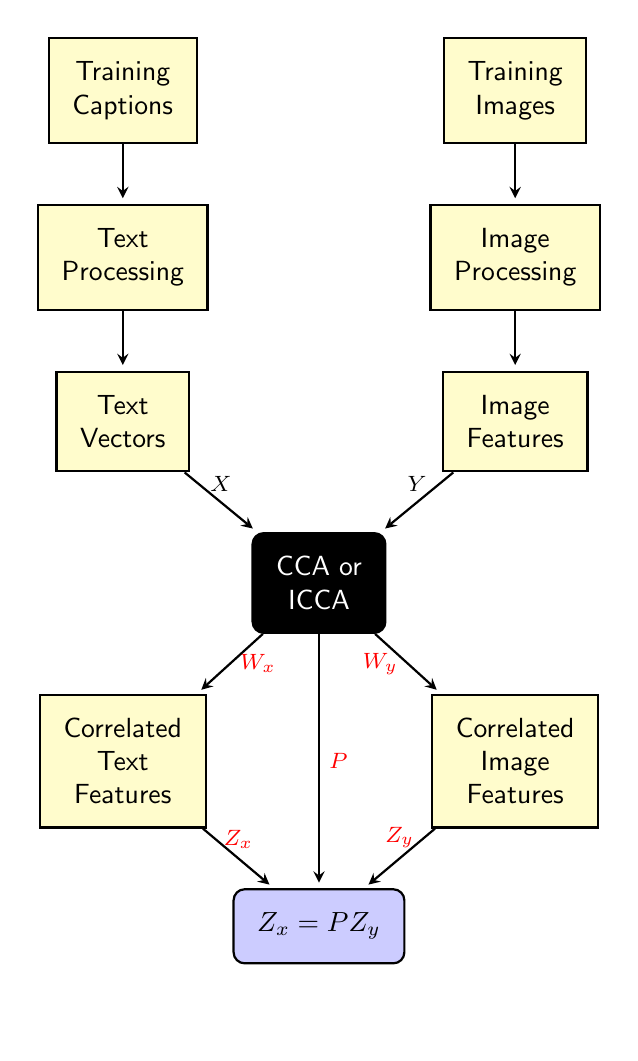
\begin{tikzpicture}[
      font=\sffamily,
      every matrix/.style={ampersand replacement=\&,column sep=2ex,row sep=5ex},
      dataset/.style={draw,thick,fill=yellow!20,inner sep=.3cm},
      sink/.style={dataset,rounded corners,fill=black, text=white},
      app/.style={dataset,rounded corners,fill=blue!20},
      dots/.style={gray,scale=2},
      to/.style={->,>=stealth,shorten >=2pt,thick,font=\sffamily\footnotesize},
      every node/.style={align=center}]

      \matrix{       
        \node[dataset] (cap) {Training \\Captions};
        \&;
        \&\node[dataset] (im) {Training \\ Images};\\

        \node[dataset] (textp) {Text \\ Processing};
        \&;
        \& \node[dataset] (imp) {Image \\Processing};\\


        \node[dataset] (dataset1) {Text \\Vectors};
        \&;
        \& \node[dataset] (dataset2) {Image \\Features};\\

        ;
        \& \node[sink] (blackbox) {CCA or\\ ICCA}; 
        \&; \\

        \node[dataset] (dataset3) {Correlated \\Text \\Features};
        \&; 
        \& \node[dataset] (dataset4) {Correlated\\ Image\\ Features};\\

        ;
        \& \node[app] (application) {$Z_x=PZ_y$};\\
        \&;\\       
      };

      \draw[to] (cap) -- (textp)node[midway,left] {};
      \draw[to] (im) -- (imp)node[midway,right] {};
      \draw[to] (textp) -- (dataset1)node[midway,left] {};
      \draw[to] (imp) -- (dataset2)node[midway,right] {};
      \draw[to] (dataset1) -- (blackbox)node[midway,above] {$X$};
      \draw[to] (dataset2) -- (blackbox)node[midway,above] {$Y$};
      \draw[to] (blackbox) -- (dataset3) node[midway,right] {\textcolor{red}{$W_x$}};
      \draw[to] (blackbox) -- (dataset4) node[midway,left] {\textcolor{red}{$W_y$}};
      \draw[to] (blackbox) -- (application) node[midway,right] {\textcolor{red}{$P$}};
      \draw[to] (dataset3) -- (application) node[midway,above] {\textcolor{red}{$Z_x$}};
      \draw[to] (dataset4) -- (application) node[midway,above] {\textcolor{red}{$Z_y$}};

    \end{tikzpicture}
    \caption{Shared training pipeline for image retrieval and annotation when using raw
      images as the second dataset. The system takes training images and captions as
      inputs and returns the canonical bases $W_x$ and $W_y$ and the correlation
      coefficients $P$.}
    \label{fig:chpt9:training}  
  \end{center}
\end{figure}

\begin{figure}[th!]
  \begin{center}
    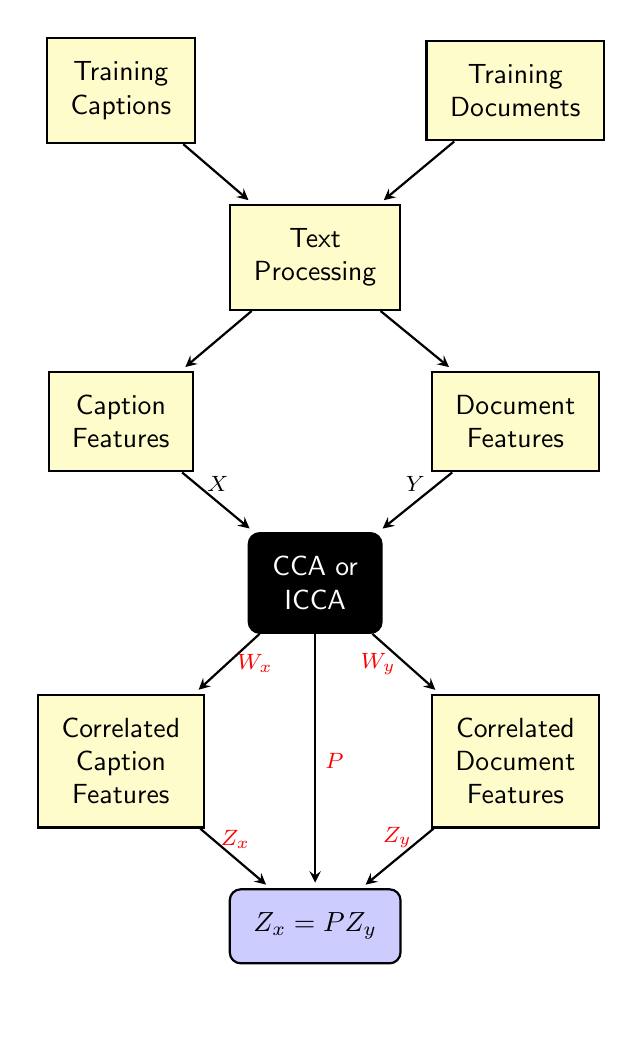
\begin{tikzpicture}[
      font=\sffamily,
      every matrix/.style={ampersand replacement=\&,column sep=2ex,row sep=5ex},
      dataset/.style={draw,thick,fill=yellow!20,inner sep=.3cm},
      sink/.style={dataset,rounded corners,fill=black, text=white},
      app/.style={dataset,rounded corners,fill=blue!20},
      dots/.style={gray,scale=2},
      to/.style={->,>=stealth,shorten >=2pt,thick,font=\sffamily\footnotesize},
      every node/.style={align=center}]

      \matrix{       
        \node[dataset] (cap) {Training \\Captions};
        \&;
        \&\node[dataset] (im) {Training \\ Documents};\\

        ;
        \&\node[dataset] (textp) {Text \\ Processing};
        \&;\\

        \node[dataset] (dataset1) {Caption \\ Features};
        \&;
        \& \node[dataset] (dataset2) {Document \\Features};\\

        ;
        \& \node[sink] (blackbox) {CCA or\\ ICCA}; 
        \&; \\

        \node[dataset] (dataset3) {Correlated \\Caption\\Features};
        \&; 
        \& \node[dataset] (dataset4) {Correlated\\ Document\\ Features};\\

        ;
        \& \node[app] (application) {$Z_x=PZ_y$};\\
        \&;\\       
      };

      \draw[to] (cap) -- (textp)node[midway,left] {};
      \draw[to] (im) -- (textp)node[midway,right] {};
      \draw[to] (textp) -- (dataset1)node[midway,left] {};
      \draw[to] (textp) -- (dataset2)node[midway,left] {};
      \draw[to] (dataset1) -- (blackbox)node[midway,above] {$X$};
      \draw[to] (dataset2) -- (blackbox)node[midway,above] {$Y$};
      \draw[to] (blackbox) -- (dataset3) node[midway,right] {\textcolor{red}{$W_x$}};
      \draw[to] (blackbox) -- (dataset4) node[midway,left] {\textcolor{red}{$W_y$}};
      \draw[to] (blackbox) -- (application) node[midway,right] {\textcolor{red}{$P$}};
      \draw[to] (dataset3) -- (application) node[midway,above] {\textcolor{red}{$Z_x$}};
      \draw[to] (dataset4) -- (application) node[midway,above] {\textcolor{red}{$Z_y$}};

    \end{tikzpicture}
    \caption{Shared training pipeline for image retrieval and annotation when the second
      dataset is associated text documents. The system takes an training captions and
      associated documents as inputs and returns the canonical bases $W_x$ and $W_y$ and
      the correlation coefficients $P$.}
  \label{fig:chpt9:training_tt}  
\end{center}
\end{figure}

\subsection{Text Processing}

Both training pipelines form feature vectors from text (either captions or documents). To
transform text into a machine understandable object, we create a feature vector whose
length is the size of the vocabulary of the training data and whose entries are tf-idf
weights. Once these vectors are created for each caption, we have a caption dataset,
$X\in\reals^{d_x\times n}$ where $d_x$ is the size of the vocabulary and $n$ is the number
of training captions associated with images. Each vector is then normalized to have an
$\ell_2$ norm of 1, so as not to penalize shorter documents. With this type of processing,
feature vector entries represent the importance that the corresponding word
carries in the document. When processing a text query for image retrieval, the text query
is transformed into a $d_x\times 1$ vector using the same tf-idf weighted scheme used to
generate the training dataset. When generating the vocabulary, we used stopword removal
and Porter stemming \footnote{http://tartarus.org/~martin/PorterStemmer/python.txt}.

\subsection{Image Processing}

The training system in Figure \ref{fig:chpt9:training} takes an image database as its second
input. To transform an image into a machine understandable object, we propose to use
visual words, which is an extension of the vector space model for text documents to
images. Here, a feature vector for an image has entries corresponding to the total
occurrences of a ``visual word'' in that image. Each visual word is a cluster of image
features extracted across all training data \cite{yang2007evaluating}. For our
implementation, we use SIFT image features vectors as the feature vectors to cluster.

The Scale Invariant Feature Transform (SIFT) was first introduced in
\cite{lowe1999object}. This algorithm transforms an image into a collection of local
feature vectors such that each feature vector is invariant to translation, scaling, and
rotation. The algorithm may be broken down into two parts. First, keypoints (pixels) are
identified using a difference-of-Gaussian function. See Figure \ref{fig:chpt9:sift} for an
example of SIFT keypoint generation. Second, a descriptor (feature vector)
is generated for each keypoint using weighted magnitude and orientation histograms in pixel
neighborhoods in a region around each keypoint. The visual word training process can be broken down into the following steps:
\begin{enumerate}
\item Create SIFT features for all training images
\item Use k-means to cluster all SIFT features into 1000 ``visual words''
\item Assign each SIFT keypoint in every image to the closest ($\ell_2$ distance) visual word
\item Count the number of occurrences of each visual word in each image
\end{enumerate}

Given the training images, the visual word image processing returns a $d_y\times n$ matrix $Y$,
where $d_y$ is the number of visual words and $n$ is the number of images. Each vector
in $Y$ is then normalized to have an $\ell_2$ norm of 1. When processing a test image for
automatic image annotation, the image's feature vector is created using the same method as
the training data.

\begin{figure}
  \centering
  \subfigure[Original Image]{
    \includegraphics[width=0.45\textwidth]{chpt9_ia/figures/orig.png}
    \label{fig:chpt9:sift_orig}}
  \subfigure[SIFT Keypoints]{
    \includegraphics[width=0.45\textwidth]{chpt9_ia/figures/sift.png}
    \label{fig:chpt9:sift_keypoints}}
  \caption{(a) Original image. (b) Original image with SIFT keypoint identification.}
  \label{fig:chpt9:sift}
\end{figure}

When creating a feature vector for a query image, we generate the SIFT features for that
image and then assign each feature to the closest visual word in the training set. Since
we create 1000 clusters, the dimension of our image feature vectors for visual words is
$d_y=1000$. We note that the visual words feature vector is highly dependent on the
training data. Each image's feature vector is dependent on the clusters found in the
training images. Therefore, we cannot pre-compute each image's feature vector without
knowing all training images.

We follow the implementation of visual words provided in \cite{solem2012programming} using
some of the code. The main changes we made were applying tf-idf weight to the visual words
and changing how we represent the vocabulary of the visual words. We also make each visual word
feature vector unit norm. For the SIFT implementation, we
use the publicly available C code at {\small{http://www.vlfeat.org/install-shell.html}}. We
made some minor changes to how the visual word implementation interfaced with the SIFT
feature creation. 

\begin{figure}
  \begin{center}
    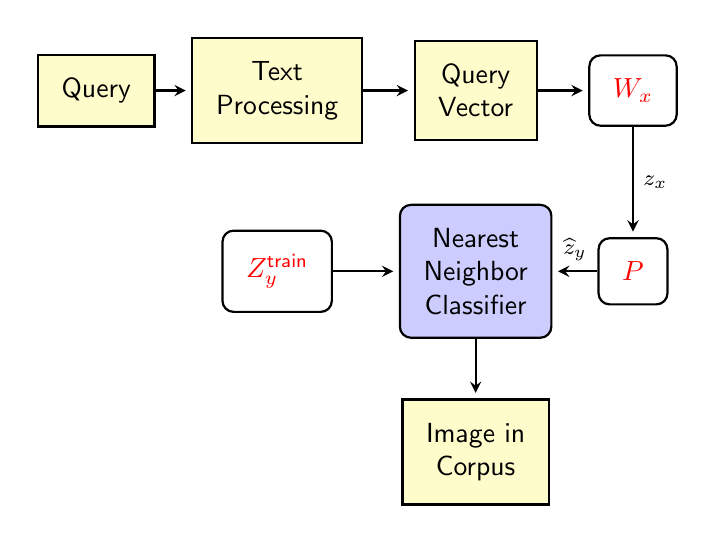
\begin{tikzpicture}[
      font=\sffamily,
      every matrix/.style={ampersand replacement=\&,column sep=3ex,row sep=5ex},
      dataset/.style={draw,thick,fill=yellow!20,inner sep=.3cm},
      sink/.style={dataset,rounded corners,fill=white, text=red},
      app/.style={dataset,rounded corners,fill=blue!20},
      dots/.style={gray,scale=2},
      to/.style={->,>=stealth,shorten >=2pt,thick,font=\sffamily\footnotesize},
      every node/.style={align=center}]

      \matrix{
        \node[dataset] (query) {Query};
        \& \node[dataset] (tp) {Text\\Processing};
        \& \node[dataset] (qv) {Query\\Vector};
        \&;\node[sink] (wx) {$W_x$};  \\

        ; 
        \& \node[sink] (zy) {$Z_y^{\text{train}}$}; 
        \& \node[app] (nn) {Nearest\\Neighbor\\Classifier};
        \& \node[sink] (P) {$P$}; \\

        ; 
        \& ;
        \& \node[dataset] (image) {Image in\\Corpus};
        \& \\
      };

      \draw[to] (query) -- (tp)node[midway,left] {};
      \draw[to] (tp) -- (qv)node[midway,right] {};
      \draw[to] (qv) -- (wx) node[midway,left] {};
      \draw[to] (wx) -- (P) node[midway,right] {$z_x$};
      \draw[to] (P) -- (nn) node[midway,above] {$\widehat{z}_y$};
      \draw[to] (zy) -- (nn) node[midway,right] {};
      \draw[to] (nn) -- (image) node[midway,right] {};


    \end{tikzpicture}
    \caption{Image retrieval pipeline. This system takes a text query as input and the
      correlation model from the training pipeline and will return relevant images.}
  \label{fig:chpt9:test1}
  \end{center}
\end{figure}

\subsection{Correlation Algorithm}

After the datasets have been processed into a caption data matrix $X$ and an image or
document data matrix $Y$, we train the CCA or ICCA as described in Section
\ref{sec:cca}. Regardless of the correlation algorithm, the output at this stage in the
training pipeline are two linear transformations $W_x\in\reals^{d_x\times k_x}$ and
$W_y\in\reals^{d_y \times k_y}$ and a diagonal matrix of canonical correlations,
$P\in\reals^{k_x\times k_y}$. The parameters $k_x$ and $k_y$ are the number of canonical
vectors to use for each dataset, respectively. As any uncorrelated canonical vectors carry
no prediction power, we simply set the number of parameters to $k=k_x=k_y$ and so $P$ is a
square matrix.

Once we learn the canonical basis vectors $W_x$ and $W_y$, we then form
the dimensionality reduced datasets of canonical variates. This is accomplished with the
simple linear transformations
\be
Z_x = W_x^TX\,\,\,\,\,\,\, Z_y = W_y^TY
\ee
where $Z_x\in\reals^{k_x\times n}$ and $Z_y\in\reals^{k_y\times n}$. These are
dimensionality reduced datasets that are maximally correlated. The beauty of these
correlation algorithms is that by solving for $W_x$, $W_y$ and $P$, we automatically solve
a regression problem in the domain of the canonical variates. This relationship is given by
\be
\E{w_x\,|\,w_y} = Pw_y \, \text{ and } \E{w_y\,|\,w_x} = Pw_x.
\ee
Notice that there is no linear offset needed as the datasets are zero mean. We also note
that this above equation is correct and that in both predictions we scale down the known
canonical variate. This makes sense by considering the following example. If $\rho_i=1$, then the
variates $w_x^{i}$ and $w_y^{i}$ are perfectly correlated and predict each other:
$w_x=w_y$. However if $\rho_i=0$, then the variates contain no information and the best
guess that we have is the mean, which is zero. For any $0<\rho_i<1$, we scale the
prediction toward zero depending on the strength of the correlation.

\begin{figure}
  \begin{center}
    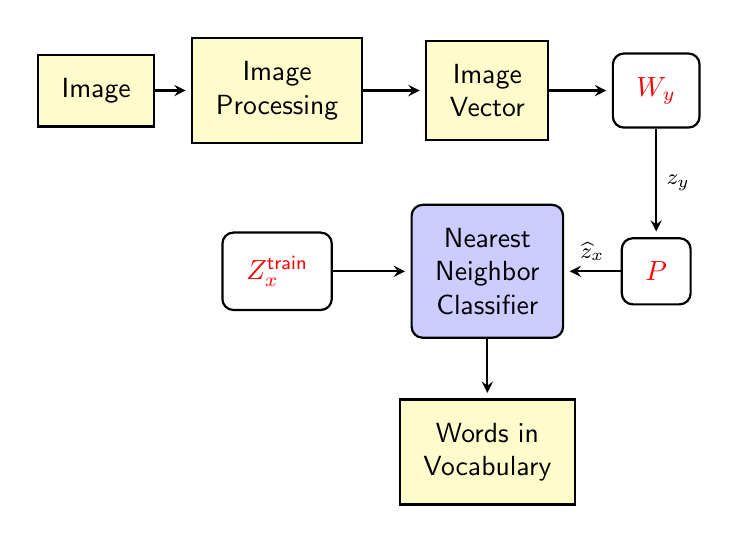
\begin{tikzpicture}[
      font=\sffamily,
      every matrix/.style={ampersand replacement=\&,column sep=3ex,row sep=5ex},
      dataset/.style={draw,thick,fill=yellow!20,inner sep=.3cm},
      sink/.style={dataset,rounded corners,fill=white, text=red},
      app/.style={dataset,rounded corners,fill=blue!20},
      dots/.style={gray,scale=2},
      to/.style={->,>=stealth,shorten >=2pt,thick,font=\sffamily\footnotesize},
      every node/.style={align=center}]


      \matrix{
        \node[dataset] (query) {Image};
        \& \node[dataset] (tp) {Image\\Processing};
        \& \node[dataset] (qv) {Image\\Vector};
        \&;\node[sink] (wx) {$W_y$};  \\

        ; 
        \& \node[sink] (zy) {$Z_x^{\text{train}}$}; 
        \& \node[app] (nn) {Nearest\\Neighbor\\Classifier};
        \& \node[sink] (P) {$P$}; \\

        ; 
        \& ;
        \& \node[dataset] (image) {Words in\\Vocabulary};
        \& \\
      };

      \draw[to] (query) -- (tp)node[midway,left] {};
      \draw[to] (tp) -- (qv)node[midway,right] {};
      \draw[to] (qv) -- (wx) node[midway,left] {};
      \draw[to] (wx) -- (P) node[midway,right] {$z_y$};
      \draw[to] (P) -- (nn) node[midway,above] {$\widehat{z}_x$};
      \draw[to] (zy) -- (nn) node[midway,right] {};
      \draw[to] (nn) -- (image) node[midway,right] {};


    \end{tikzpicture}
    \caption{Image annotation pipeline when using the raw image as input. This system
      takes an image and correlation model from the training system as inputs and will
      return a list of words that are most relevant for the image.}
  \label{fig:chpt9:test2}
  \end{center}
\end{figure}

\begin{figure}
  \begin{center}
    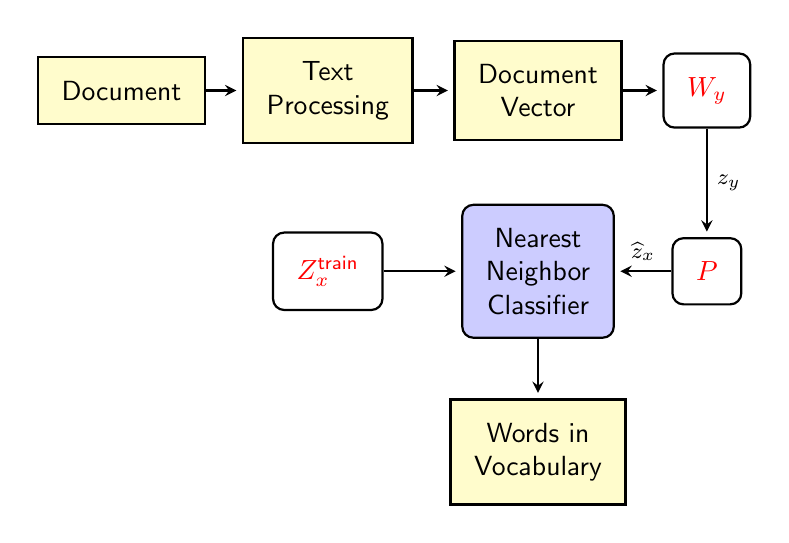
\begin{tikzpicture}[
      font=\sffamily,
      every matrix/.style={ampersand replacement=\&,column sep=3ex,row sep=5ex},
      dataset/.style={draw,thick,fill=yellow!20,inner sep=.3cm},
      sink/.style={dataset,rounded corners,fill=white, text=red},
      app/.style={dataset,rounded corners,fill=blue!20},
      dots/.style={gray,scale=2},
      to/.style={->,>=stealth,shorten >=2pt,thick,font=\sffamily\footnotesize},
      every node/.style={align=center}]


      \matrix{
        \node[dataset] (query) {Document};
        \& \node[dataset] (tp) {Text\\Processing};
        \& \node[dataset] (qv) {Document\\Vector};
        \&;\node[sink] (wx) {$W_y$};  \\

        ; 
        \& \node[sink] (zy) {$Z_x^{\text{train}}$}; 
        \& \node[app] (nn) {Nearest\\Neighbor\\Classifier};
        \& \node[sink] (P) {$P$}; \\

        ; 
        \& ;
        \& \node[dataset] (image) {Words in\\Vocabulary};
        \& \\
      };

      \draw[to] (query) -- (tp)node[midway,left] {};
      \draw[to] (tp) -- (qv)node[midway,right] {};
      \draw[to] (qv) -- (wx) node[midway,left] {};
      \draw[to] (wx) -- (P) node[midway,right] {$z_y$};
      \draw[to] (P) -- (nn) node[midway,above] {$\widehat{z}_x$};
      \draw[to] (zy) -- (nn) node[midway,right] {};
      \draw[to] (nn) -- (image) node[midway,right] {};


    \end{tikzpicture}
    \caption{Image annotation pipeline when using associated text documents. This system
      takes a text document and correlation model from the training system as inputs and will
      return a list of words that are most relevant for the associated image.}
  \label{fig:chpt9:test3}
  \end{center}
\end{figure}


\subsection{Image Retrieval}

After training the system on a corpus, a user may perform image retrieval. Given a text
query, we first process it using the same tf-idf weighting scheme used in the training
model, resulting in the vector $q\in\reals^{d_x\times 1}$. To obtain an estimate of our
image feature, we perform the following sequence of linear transformations, learned by one
of the correlation algorithms,
\be
\widehat{z}_y = PW_x^Tq
\ee
To return relevant images, we use a nearest neighbor classifier in the canonical variate
domain. We can pre-compute all possible images to return via $Z_y^{\text{train}} = W_y^TY$.
The output of the search is 
\beq\label{eq:chpt9:ir_scores} y_{\text{guess}} =
\argmin_{z_y\in Z_y^{\text{train}}}
\|z_y-\widehat{z}_y\|_2^2,
\eeq
which is repeated for as many results the user desires, excluding previously returned
results from the search set each time. A nice benefit of using correlation methods is that
additional images may be added to the set of returnable images, even if they do not have a
caption associated with them. All we need is the low dimensional representation of these
additional images using the transformation learned from the training set, whether that be
image features or document vectors.

\subsection{Image Annotation}

The trained system can also handle automatic image annotation. Given a query image or
associated document, we
first process it using the same image or text processing that was used in training, resulting in a
query vector $q\in\reals^{d_y\times 1}$. To obtain an estimate of our text features, we
perform the following linear transformation
\be
\widehat{z}_x = PW_y^Tq
\ee
using the correlation model learned in the training phase. To return relevant words, we
use a nearest neighbor classifier in the canonical variate domain. However, instead of
using the captions as the vectors to compare against, we consider $d_x$ documents, each of
which contains exactly one of the words in the vocabulary. Let $D\in\reals^{d_x\times
  d_x}$ be a diagonal matrix with entries equal to the tf-idf score of that word. Define
$Z_x^{\text{train}}=W_x^TD$ to be the canonical variate vectors of each word. Then the output of the
nearest neighbor classifier is
\beq\label{eq:chpt9:ia_scores} x_{\text{guess}} =
\argmin_{z_x\in Z_x^{\text{train}}}
\|z_D-\widehat{z}_x\|_2^2.
\eeq 
We then return the words corresponding to the vectors returned by the nearest neighbor
classifier.

\section{Experiments}\label{sec:results}

To compare the performance of CCA and ICCA in image retrieval and annotation, we test our
system on four different datasets. For the Pascal Image Dataset, we wrote a command line
interface to perform both image retrieval and image annotation. This allows for us to
qualitatively determine how each method works. For the University of Washington Ground
Truth dataset, we run the training and testing pipelines in Figures
\ref{fig:chpt9:training} and \ref{fig:chpt9:test2} and compare the R-precision for the
image annotation task. For the Gold Standard Web dataset, we only have a few image-caption
pairs but also have associated text documents and so we use the training pipelines in
Figures \ref{fig:chpt9:training_tt} and \ref{fig:chpt9:test3}. We compare our eigen-based
annotation methods to previous NLP methods using the evaluation framework in
\cite{leong2010text}. Finally, we use the training pipelines in Figures
\ref{fig:chpt9:training_tt} and \ref{fig:chpt9:test3} to test the image annotation
performance of CCA and ICCA on the BBC News dataset. This dataset is particularly
challenging first because the images are extremely varied and may only be tangentially
related to the associated document, and second because the accompanying caption is often
extremely nuanced, containing few keywords. These challenges present many latent
variables, which CCA and ICCA will not handle very well.

\subsection{Pascal Image Dataset}

\begin{figure}[t]
  \begin{minipage}{0.45\linewidth}
    \centering
    \includegraphics[width=.8\textwidth]{chpt9_ia/figures/img_3.jpg}
  \end{minipage}
  \begin{minipage}[t]{0.45\linewidth}
    \vspace{-1in}
    \centering
    \footnotesize
    \begin{itemize}
    \item A D-ERFW-6 in flight.
    \item An army green plane flying in the sky.
    \item An old fighter plane flying with German military markings.
    \item A small green and yellow plane in the sky.
    \item A WWII fighter plane with its landing gear down.
    \end{itemize}
  \end{minipage}
  \caption{Example of an image and its captions in the Pascal dataset}
  \label{fig:chpt9:pascal}
\end{figure}

The Pascal Image dataset
\footnote{http://nlp.cs.illinois.edu/HockenmaierGroup/pascal-sentences/} was created using
Amazon's Mechanical Turk \cite{rashtchian2010collecting}. The dataset consists of 1000
images, each with 5 captions. The average image has 26.67 caption words and the total
vocabulary size of the corpus is 2393. The 5 captions for each image are unique, but they
may repeat keywords or use synonyms.  For example, airplanes in the dataset can be
described as airplanes, planes, fighter planes, jets, and even their model. See Figure
\ref{fig:chpt9:pascal} for an example image-caption pair.

\begin{figure}[t]
  \centering
  \subfigure[CCA Results]{
    \centering
    \includegraphics[width=0.45\textwidth]{chpt9_ia/figures/pascal_cca_ex.png}
    \label{fig:chpt9:CCA_query_results}}
  \subfigure[ICCA Results]{
    \centering
    \includegraphics[width=0.45\textwidth]{chpt9_ia/figures/pascal_icca_ex.png}
    \label{fig:chpt9:ICCA_query_results}}
  \caption{(a) CCA results for query "airplane". (b) ICCA results for query "airplane".}
  \label{fig:chpt9:pascal_results}
\end{figure}

\begin{figure}[t]
  \centering
  \subfigure[CCA Results]{
    \centering
    \includegraphics[width=0.45\textwidth]{chpt9_ia/figures/cca_ir.png}
    \label{fig:chpt9:cca_ir}}
  \subfigure[CCA Results Zoomed]{
    \centering
    \includegraphics[width=0.45\textwidth]{chpt9_ia/figures/cca_ir_zoom.png}
    \label{fig:chpt9:cca_ir_zoom}}
  \subfigure[ICCA Results]{
    \centering
    \includegraphics[width=0.45\textwidth]{chpt9_ia/figures/icca_ir.png}
    \label{fig:chpt9:icca_ir}}
  \subfigure[ICCA Results Zoomed]{
    \centering
    \includegraphics[width=0.45\textwidth]{chpt9_ia/figures/icca_ir_zoom.png}
    \label{fig:chpt9:icca_ir_zoom}}
  \caption{(a) Scores for all 1000 Pascal images for the query ``airplane'' for CCA. (b)
    Zoomed in version of (a) to highlight the top scores returned in Figure
    \ref{fig:chpt9:CCA_query_results}. (c) Scores for all 1000 Pascal
    images for the query ``airplane'' for ICCA. (d) Zoomed in version of (c) to highlight
    the top scores which are returned in Figure \ref{fig:chpt9:ICCA_query_results}. All
    scores are the norm in (\ref{eq:chpt9:ir_scores}).}
  \label{fig:chpt9:pascal_ir}
\end{figure}

To qualitatively evaluate the performance of CCA and ICCA using visual words, we
implemented the image retrieval and image annotation systems described in Section
\ref{sec:propose}. Figure \ref{fig:chpt9:pascal_results} shows the first four images
retrieved for the search query ``airplane'' using both CCA and ICCA correlation models. We
plot the scores used to return these images in Figure \ref{fig:chpt9:pascal_ir}. The
largest four scores correspond to the images in Figure \ref{fig:chpt9:pascal_results} as
computed via (\ref{eq:chpt9:ir_scores}). Figure \ref{fig:chpt9:pascal_annotation} shows
the first ten words returned for the image in Figure \ref{fig:chpt9:pascal_query_image},
which was taken from the Pascal dataset. Figure \ref{fig:chpt9:pascal_ia} plots the
corresponding scores for all words in the database as computed via
(\ref{eq:chpt9:ia_scores}). The top scores correspond to the words returned in Figure
\ref{fig:chpt9:pascal_annotation}. For both tasks, we used all 1000 image-caption pairs in
the Pascal dataset for training. Thus, any image in the dataset may be returned in the
image retrieval task. Similarly, any Porter-stemmed vocabulary word in the entire caption
dataset may be returned in the image annotation task.

\begin{figure}[t]
	\centering
	\subfigure[Image Query] {
	\includegraphics[width=0.4\textwidth]{chpt9_ia/figures/img_27.jpg}
	\label{fig:chpt9:pascal_query_image}}

	\subfigure{
    \begin{minipage}[t]{0.3\textwidth}
      \small
      \begin{center}
        \textbf{CCA Annotation}
      \end{center}
      \begin{enumerate}
      \item hairless
      \item buddi
      \item swan
      \item leaf-less
      \item bnsf
      \item desert
      \item fluffi
      \item salad
      \item majest
      \item memorabilia
      \end{enumerate}
    \end{minipage}%
    \begin{minipage}[t]{0.2\textwidth}
    \end{minipage}
    \begin{minipage}[t]{0.3\textwidth}
      \small
      \begin{center}
        \textbf{ICCA Annotation}
      \end{center}
      \begin{enumerate}
      \item plane
      \item ship
      \item cruis
      \item fly
      \item blue
      \item jet
      \item airplan
      \item dock
      \item fighter
      \item through
      \end{enumerate}
    \end{minipage}}
	\caption{CCA vs ICCA annotation results for the image query shown in
      \ref{fig:chpt9:pascal_query_image}.}
    \label{fig:chpt9:pascal_annotation}
\end{figure}

\begin{figure}[t]
  \centering
  \subfigure[CCA Results]{
    \centering
    \includegraphics[width=0.45\textwidth]{chpt9_ia/figures/cca_ia.png}
    \label{fig:chpt9:cca_ia}}
  \subfigure[CCA Results Zoomed]{
    \centering
    \includegraphics[width=0.45\textwidth]{chpt9_ia/figures/cca_ia_zoom.png}
    \label{fig:chpt9:cca_ia_zoom}}
  \subfigure[ICCA Results]{
    \centering
    \includegraphics[width=0.45\textwidth]{chpt9_ia/figures/icca_ia.png}
    \label{fig:chpt9:icca_ia}}
  \subfigure[ICCA Results Zoomed]{
    \centering
    \includegraphics[width=0.45\textwidth]{chpt9_ia/figures/icca_ia_zoom.png}
    \label{fig:chpt9:icca_ia_zoom}}
  \caption{(a) CCA scores for all words in the Pascal database for the image query in
    Figure \ref{fig:chpt9:pascal_query_image}. (b) Zoomed in version of (a) to highlight
    the top scores returned in Figure \ref{fig:chpt9:pascal_annotation}. (c) ICCA scores
    for all words in the Pascal database for the image query in Figure
    \ref{fig:chpt9:pascal_query_image}. (d) Zoomed in version of (c) to highlight the top
    scores which are returned in Figure \ref{fig:chpt9:pascal_annotation}. All
    scores are the norm in (\ref{eq:chpt9:ia_scores}).}
  \label{fig:chpt9:pascal_ia}
\end{figure}

\subsection{Ground Truth Image Dataset}

To quantitatively compare the performance of CCA and ICCA, we used the University of
Washington Ground Truth Image Dataset
\footnote{http://www.cs.washington.edu/research/imagedatabase/groundtruth/}. This
dataset contains 1109 images with an average of 5.57 keywords per image and a total of 346
unique words. We randomly split the dataset into 3 sets: a training set of 550 images, a
validation set of 250 images and a testing set of 309 images. This was repeated to obtain
10 such partitions.

For each partitioning, the training dataset was used to learn the correlation model for
CCA, and ICCA. This model was learned for values of $k=$10,25,50,75,100.  The validation
dataset was then used to determine the best value of $k$ for each algorithm, using
R-precision as our evaluation metric. In this setting, R-precision is equal to the
percentage of correctly predicted keywords for an image. Once the best $k$ was determined,
that partition's R-precision value for each algorithm was determined on the testing
datasets. The R-precision values were then averaged across partitions. Figure
\ref{fig:chpt9:gt_rprec} plots the probability density function of R-precision for CCA and
ICCA and Table \ref{table:rprec} shows the mean R-precision and average $k$
values.

\begin{figure}[t]
  \centering
  \subfigure[CCA]{
    \includegraphics[width=0.45\textwidth]{chpt9_ia/figures/cca_rprec_vw.png}
    \label{fig:chpt9:rprec_cca_vw}}
  \subfigure[ICCA]{
    \includegraphics[width=0.45\textwidth]{chpt9_ia/figures/icca_rprec_vw.png}
    \label{fig:chpt9:rprec_icca_vw}}
  \caption{Empirical probability density functions of R-precision of image annotation of
    the University of Washington Ground Truth Dataset.}
  \label{fig:chpt9:gt_rprec}
\end{figure}

\begin{table}[t]
\centering
\begin{tabular}{c||c|c}
& Mean R-precision& Mean $k$\\ \hline
CCA &  0.024& 63\\
ICCA & 0.232& 20\\
\bottomrule
\end{tabular}
\caption{Average R-precision values and correlation basis dimension, $k$, for image
  annotation of the University of Washington  Ground Truth Dataset }
\label{table:rprec}
\vspace{-0.1in}
\end{table}

\subsection{Gold Standard Web Dataset}

Next, we evaluate our eigen-based image annotation methods on the Gold Standard Web
Dataset \cite{leong2010text}. This dataset contains 300 image-text pairs that was
collected from the web. The average text document length is 278 tokens and the vocabulary
size is 8,409 words. Each image also has a gold standard of manually assigned tags labeled
by five human annotators. We consider these manually assigned tags as the
caption. However, as we only have 300 images and these images contain many different
objects, we use the associated text document  as the second
modality. Hence, our goal is to predict the captions given the text document, which is
essentially keyword identification.

We use the same four evaluation metrics as \cite{leong2010text} to be able to make direct
comparisons with previous methods. As CCA and ICCA can return an arbitrary number of
keywords, we choose to always predict keywords equal to the number of true
keywords. Therefore, for our methods, these metrics are variations on R-precision. Some
images are considered Mode images when there is a unique keyword selected by more
annotators than any other keyword. The metrics are given in Table
\ref{table:gold_metrics}. Let $\mathcal{I}$ be the set of all images, $\mathcal{IM}$ be
the set of mode images, $f_i^j$ be the number annotators who labeled image $i$ with keyword
$j$, $r_i$ be the number of keywords selected for image $i$, and $R_i=\sum_{j=1}^{r_i}f_i^j$. Table \ref{table:gold}
reports the performance of CCA and ICCA in generating keywords given these 4 metrics using
leave-one-out testing. We also provide the performance of models used in
\cite{leong2010text} for comparison.

\begin{table}[t]
  \centering
  \begin{tabular}{l|l}
    Metric & Expression\\
    \midrule
    Best Normal & $\frac{1}{|\mathcal{I}|}\sum_{i\in\mathcal{I}}\frac{1}{r_iR_i}\sum_{j=1}^{r_i}f_i^j$\\
    Best Mode & $\frac{1}{|\mathcal{IM}|}\sum_{i\in\mathcal{IM}}\indicator_{\left\{\text{top tag = mode}\right\}}$\\
    oot Normal & $\frac{1}{|\mathcal{I}|}\sum_{i\in\mathcal{I}}\frac{1}{R_i}\sum_{j=1}^{r_i}f_i^j$\\
    oot Mode & $\frac{1}{|\mathcal{IM}|}\sum_{i\in\mathcal{IM}}\indicator_{\left\{\text{any tag = mode}\right\}}$\\
    \bottomrule
  \end{tabular}
  \caption{Image annotation for the Web Image-Article dataset.}
  \label{table:gold_metrics}
  \vspace{-0.1in}
\end{table}


\begin{table}[t]
\centering
\begin{tabular}{l|cc|cc}
Models & Best Normal & Best Mode & oot Normal & oot Mode\\\hline
CCA & 0.01 & 0.00 & 1.49 & 35.23\\
ICCA & 0.19 & 9.09 & 16.11 & 76.7 \\
\midrule
\midrule
Flickr picturability & 6.32 & 78.57 & 35.61 & 92.86\\
Wikipedia Salience & 6.40 & 7.14 & 35.19 & 92.86 \\
Topic modeling & 5.99 & 42.86 & 37.13 & 85.71 \\
\midrule
\midrule
Doc Title & 6.40 & 75.00 & 18.97 & 82.14\\
tf*idf & 5.94 & 14.29 & 38.40 & 78.57\\
\bottomrule
\end{tabular}
\caption{Image annotation for the Web Image-Article dataset.}
\label{table:gold}
\vspace{-0.1in}
\end{table}


\subsection{BBC News Dataset}

Finally, we evaluate CCA and ICCA based image annotation on the BBC News dataset
\cite{feng2008automatic}. Similar to the Gold Standard Web dataset, this dataset contains
image-caption-document tuples that are separated into 3121 training examples and 240
testing examples. The images in this dataset are again very varied and the captions are
sometimes nuanced and very specific to the image and not very related to the accompanying
document. For the CCA and ICCA annotations, we again will use the accompanying documents
to predict keywords in the caption. We report the precision and recall when returning the
top 10, 15 and 20 predicted keywords in Table \ref{table:bbc}. In the table we also report
methods from \cite{feng2008automatic} and \cite{leong2010text} for comparison.  We follow
implementations reported in \cite{feng2008automatic} and \cite{leong2010text} to not
Porter stem the words but instead use Tree Tagger\cite{schmid1994probabilistic} to include
only nouns, verbs, and adjectives.

\begin{figure}[t]
  \begin{minipage}{0.45\linewidth}
    \centering
    \includegraphics[width=.8\textwidth]{chpt9_ia/figures/bbc_img.jpg}
  \end{minipage}
  \begin{minipage}{0.45\linewidth}
    \centering
    \footnotesize
    \textbf{Caption}
    \begin{itemize}
    \item Agreement came despite reservations on both sides
    \end{itemize}
    \textbf{Title}
    \begin{itemize}
    \item UN Secretary General Kofi Annan has called on the Sudanese government to allow a
      UN assessment team into the war-torn region of Darfur
    \end{itemize}
  \end{minipage}
  \caption{Example of an image, its caption, and title in the BBC News dataset}
  \label{fig:chpt9:bbc_ex}
\end{figure}


\begin{table}[t]
\centering
\begin{tabular}{l|cc|cc|cc}
& \multicolumn{2}{|c|}{Top 10} & \multicolumn{2}{|c|}{Top 15} & \multicolumn{2}{|c|}{Top
  20}\\
Models & P & R & P & R & P & R\\ 
\midrule
CCA & 0.08 & 0.11 & 0.08 & 0.22 & 0.08 & 0.28\\
ICCA & 0.79 & 1.48 & 0.72 & 1.95 & 0.73 & 2.63\\
\midrule
\midrule
tf*idf & 4.37 & 7.09 & 3.57 & 8.12 & 2.65 & 8.89\\
DocTitle & 9.22 & 7.03 & 9.22 & 7.03 & 9.22 & 7.03\\
Lavrenko03 & 9.05 & 16.01 & 7.73 & 17.87 & 6.55 & 19.38\\
ExtModel & 14.72 & 27.95 & 11.62 & 32.99 & 9.72 & 36.77\\
\midrule
\midrule
Flickr picturability & 12.13 & 22.82 & 9.52 & 26.82 & 8.23 & 29.80\\
Wikipedia Salience & 11.63 & 21.89 & 9.28 & 26.20 & 7.81 & 29.41\\
Topic Modeling & 11.42 & 21.49 & 9.28 & 26.20 & 7.86 & 29.57\\
\bottomrule
\end{tabular}
\caption{Image annotation for the Web Image-Article dataset.}
\label{table:bbc}
\vspace{-0.1in}
\end{table}

\section{Discussion}\label{sec:disc}
\subsection{Pascal Results}

For the Pascal dataset, we can qualitatively see the performance increase that ICCA
gives. Examining Figure \ref{fig:chpt9:CCA_query_results}, we see that CCA returns random
images associated with the query ``airplane''. This is the case with any other query
entered.  However this is expected with CCA as it returns a correlation of 1 between all
images and tokens as we are operating in the sample deficient regime.  Any positive
results returned by CCA can be attributed to random luck. On the other hand, using ICCA to
train a retrieval system results in better overall performance than CCA. This can be seen
specifically in Figure \ref{fig:chpt9:ICCA_query_results}, which shows images for the same
query of ``airplane''. Using ICCA, two of the first four results are planes. By only using
\textit{informative} singular vectors, ICCA is able to return more relevant images.

Specifically, if we examine Figure \ref{fig:chpt9:pascal_ir}, we can compare the scores
returned for each image for CCA and ICCA. The top scores for ICCA seem to separate from
the bulk of the others, while for CCA, the top scores seem to be part of the bulk
distribution. This gives support to the notion that ICCA is able to identify images that
are relevant to the desired keyword.

Image annotation using CCA also returns random keywords for any image query. An example of
this is shown in Figure \ref{fig:chpt9:pascal_annotation}. The query image is an airplane but
the top 10 words returned by CCA are all irrelevant. This once again reinforces the idea
that CCA only returns random results in the sample deficient regime. However, examining
the top 10 words returned by ICCA for the same image, we observe meaningful annotations
such as ``plane'', ``blue'', ``fly''. Examining Figure \ref{fig:chpt9:pascal_ia}, we see the
corresponding scores to the words returned in Figure
\ref{fig:chpt9:pascal_annotation}. Again we notice that a majority of the words fall into
the bulk distribution for CCA and ICCA. The words in the bulk part of the distribution are
not informative. However, in ICCA, there are a number of words that separate from the bulk
distribution, which we show in Figure \ref{fig:chpt9:pascal_annotation}. However, the
scores for CCA do not separate as nicely from the distribution. This further gives support
that CCA randomly returned words/images in the sample deficient regime.

A \naive image retrieval system may perform a search using only the captions and then
return the image associated with the most notable caption. This produces very good results
for the Pascal dataset because the captions are very clean and noise-free. Every caption
with the word sheep will have a sheep in the image. However, correlation based approaches
have a few main advantages over such a \naive method. First, correlation methods solve
both the image retrieval and image annotation problem simultaneously. The \naive image
retrieval method cannot solve the image annotation problem. Second, correlation methods
can handle adding images to the corpus post training, even if it does not have an
associated caption. For the image retrieval problem, the correlation methods will return
images with low-dimensional representation that are close to the predicted vector. Adding
additional images (even without captions) requires transforming the images into the
low-dimensional representation using the trained transformation and then adding them to
the set of possible images to be returned. The \naive method needs a caption for every
image and if a new image-caption pair was added, the entire inverted index and vocabulary
would need to be recomputed.


\subsection{Image Annotation of Ground Truth Dataset}

We use the Ground Truth Dataset to provide a more quantitative comparison of CCA and ICCA
based image annotation. The captions for this dataset only consist of keywords and is
thus easier to assess the quality of the image annotations. We did not clean up the
dataset by removing misspelled words or words appearing only once. Therefore, the reported
results are a nice lower-bound that one could expect by doing such clever pre-processing
steps. As evident in Table \ref{table:rprec}, CCA performs very poorly on the image
annotation task. This R-precision corresponds to random guessing, which matches the
results of \cite{pezeshki2004empirical} stating that in the sample starved regime, the CCA
bases are random projections. However, using ICCA to informatively trim data matrices
results in improved annotations. Examining the figures in Figure \ref{fig:chpt9:gt_rprec}, we
see that when using CCA, approximately 85\% of the images result is an R-precision of
0. However, ICCA returns zero relevant images only 35\% of the time. Clearly, ICCA is able
to uncover true correlations to return relevant annotations. This gives credence to using
correlation methods for image annotation tasks.

\subsection{Annotation of Gold Standard Web Dataset}

The Gold Standard Web dataset is a more difficult dataset than the Ground Truth
dataset. First, there are only 300 examples in the dataset. Using leave-one-out testing
gives a training dataset of only 299 examples. Second, the dimensions of our dataset
increases because we use tf-idf weights from the associated documents instead of visual
words from the image. Therefore, we are in a very sample deficient regime where our
dimension of each dataset is on the order of 8000 and we only have 299
samples. Compounding issues, these vectors are very sparse as documents only have a subset
of the total words in the vocabulary. However, ICCA is indeed able to recover meaningful
annotations even in this regime.

Examining the difference between the Best Mode and oot Mode performance metrics, we see
that ICCA has a very large gap. This indicates that the ICCA retrieval method is very
often able to retrieve the mode annotation, just not label it as the best annotation. 

\subsection{Annotation of BBC News Dataset}

The BBC News dataset is the most difficult dataset we consider in this chapter. Here, we
have a large number of training data, however, our captions are very ``noisy''. Unlike the
Gold Standard Web dataset, the BBC captions may contain words that do not appear in the
accompanying document. These captions are also very nuanced and may describe an image that
is only tangentially related to the main article. For example, consider Figure
\ref{fig:chpt9:bbc_ex}. The image is of two men shaking hands, however, the caption
describes this very abstractly. In addition, the caption highlights a very subtle point of
the main article, as we can see by the title. Similar to the Gold Standard Web dataset,
our feature vectors are both very high dimensional and sparse. We see from the results in
Table \ref{table:bbc} that both CCA and ICCA do a poor job at retrieving relevant
annotations given the BBC article. However, we do observe the behavior that CCA returns
completely random results and ICCA is able to perform slightly better (non-randomly).

The BBC News dataset breaks many of the assumptions of ICCA and therefore causes its
performance to decrease. First, the dataset breaks the linear correlation assumption of
ICCA. As we saw in Figure \ref{fig:chpt9:bbc_ex}, captions are can be very nuanced, indicating
many latent variables interacting in most likely nonlinear ways. Due to the size of the
vocabulary of the BBC dataset, our text feature vectors are incredibly sparse, which as we
saw in previous chapters, requires a larger SNR to detect correlations. The nonlinear
correlations most certainly decrease the SNR in our dataset, which, coupled with the
sparse data, stretches ICCA based image annotation to the limit of decent operation. 

Clever feature engineering and alterations of ICCA could yield potential new avenues to
improve the performance on difficult datasets such as the BBC News dataset. One possible
extension is to use a kernel version of ICCA to account for nonlinear
correlations. Similarly, extending ICCA to better handle sparse vectors could improve
performance. Finally, using more intelligent IR and NLP techniques to create more
informative feature vectors than tf*idf weights could increase the relative SNR high
enough to allow for more reliable correlation detection.

\section{Conclusion}\label{sec:conc}

In this chapter, we applied CCA and ICCA based correlation detection methods to image
retrieval and annotation. By trimming data matrices to only include informative subspace
components, ICCA is able to avoid the performance loss of CCA in the sample deficient
regime. We demonstrated through multiple datasets that ICCA is able to outperform CCA on
both image retrieval and image annotation tasks, both qualitatively and
quantitatively. 

For all datasets, CCA failed completely while ICCA was able to return meaningful
results. Depending on the difficulty of the dataset, the performance of ICCA ranged from
acceptable (Ground Truth dataset) to poor (BBC News Dataset). The more difficult datasets
tend to break many of the assumptions that ICCA makes. The vectors in these datasets are very
sparse, which ICCA does not account for directly. ICCA is also a linear method and so any
nonlinear correlations will not be detected. For these more difficult datasets, the
captions contained very nuanced language or words not even used in the main article. 

The purpose of this chapter is to spark a discussion for using eigen-based correlation
methods for image annotation, image retrieval, and possibly other NLP
problems. While ICCA performs worse than the current NLP techniques it is able to capture
underlying meaning between words and images. By applying NLP techniques to create better
feature vectors than tf*idf weights and extending ICCA to allow for non-linear sparse
correlations, one could hope for improved performance. While CCA was rightfully overlooked
as a possible solution to such information retrieval problems, we hope that practitioners will
reconsider eigen-based correlation approaches in the future.



\chapter{Multiset CCA (MCCA)}\label{sec:chpt_mcca}
\section{Introduction}
Multi-modal data fusion is a ubiquitous problem in signal processing and machine
learning. In many applications, we have access to multiple datasets, possibly of different
modalities, each of which describe some feature of the system. This setup is becoming
increasingly common today as data collection becomes cheaper and easier. We are no longer
limited by the amount or variety of data that we can collect, but instead by how quickly
and accurately we can process such a wide variety of data. Access to more
than two datasets arises in applications such as handwritten digit classification
\cite{yu2007learning}, multi-temporal hyperspectral imaging \cite{nielsen2002multiset},
and medical imaging \cite{correa2010canonical, deleus2011functional}.

Unlike the two dataset case, there is not a singular definition for correlation between
more than two random variables. Kettenring \cite{kettenring1971canonical} considers five
such definitions that extend Hotellings's \cite{hotelling1936relations} original canonical
correlation analysis (CCA) work. These five formulations of multiset CCA (MCCA) unify
multiset correlation analysis of the previous decades \cite{vinograde1950canonical,
  steel1951minimum, horst1961relations, horst1961generalized}. Nielsen
\cite{nielsen1994analysis} later extended Kettenring's analysis by also considering four
constraint functions placed on the canonical vectors in the optimization problem.

In this paper consider the performance of one MCCA optimization problem, MAXVAR. We show
that, similar to empirical CCA, the solution to this problem is a SVD of a matrix with block
entries of the pairwise product of right singular vectors of the individual datasets. We
then apply the same principles used in informative CCA (ICCA) to develop an informative version of MAXVAR,
which we call IMCCA. Using the idea of trim-then-fuse, we propose to trim all data SVDs to
include only the \textit{informative} singular vectors. We provide some analysis of the
behavior of these algorithms and provide a test statistic to use to determine the number
of correlations present in multiple datasets. We discuss why multi-dataset correlation
analysis is difficult but showcase on a real world dataset that IMCCA greatly outperforms
MAXVAR and can robustly identify sources of correlation.


\section{Mathematical Formulation of MCCA}

Let $y_1,y_2,\dots,y_m$ be observations drawn from $m$ distributions $y_i\sim
\mathcal{Y}_i$ with $y_i\in\complex^{d_i}$. Assume, without loss of generality, that $y_i$
is zero mean. Define the covariance between distributions as $\E{y_iy_j^T}=R_{ij}$ for
$i,j=1,\dots,m$. Define the joint observation vector $y$ and its covariance $R=\E{yy^H}$ as
\be
y = \left[\begin{array}{c}y_1\\ \vdots \\ y_m\end{array}\right] \in\complex^{d\times 1},\,\,\,\,R
= \left[\begin{array}{ccc}R_{11}&\dots&R_{1m}\\ \vdots&\ddots&\vdots\\ 
    R_{m1}&\dots&R_{mm}\end{array}\right]\in\complex^{d\times d}
\ee
where $d=\sum_{i=1}^md_i$.

The goal of MCCA is to find canonical coefficient vectors, $x_i\in\complex^{d_i\times 1}$
for $i=1,\dots,m$, such that the canonical variates, $w_i=x_i^Hy_i$, are optimal with
respect to an objective function $J(\cdot)$ and constraint function $h(\cdot)$. Define the
vector of canonical vectors as 
$x=\left[x_1^H,\dots,x_m^H\right]^H\in\complex^{d\times 1}$ and the vector of canonical
variates as $w=[w_1,\dots,w_m]^H\in\complex^{m\times 1}$. The covariance matrix of $w$ is
\begin{equation*}
\Phi(x)=\E{ww^H}=\left[\begin{array}{ccc} x_1^HR_{11}x_1 & \dots & x_1^HR_{1m}x_m \\ \vdots
    & \ddots & \vdots \\ x_m^HR_{m1}x_1 & \dots & x_m^HR_{mm}x_m\\ \end{array}\right].
\end{equation*}
Using this notation, the MCCA optimization problem is
\begin{equation}\label{eq:chpt10:opt_prob}
\begin{aligned}
&\underset{x}{\mathop{\rm optimize}} && J(\Phi(x))\\
&\text{subject to} && h(x,R).\\
\end{aligned}
\end{equation}
For this paper we consider the maximum variance (MAXVAR) objective function with the
constraint functions
  \begin{equation*}
    x_i^HR_{ii}x_i = 1,\, 1\leq i\leq m,
  \end{equation*}
which require the canonical variate to be unit norm.

\subsection{Solution to MAXVAR}
The MAXVAR optimization problem is
\begin{equation*}
\begin{aligned}
&\argmax_{x}&&\lambda\\
&\text{s.t.} &&x_i^HR_{ii}x_i  = 1\,\,,1\leq i\leq m\\
&&& \Phi(x) a = \lambda a\\
&&& a^Ha=1.\\
\end{aligned}
\end{equation*}
Writing $\Phi(x) = X^H R X$, where $X=\blkdiag(x_1,\dots,x_m)$, and making the
transformation $\widetilde{a}=R_D^{1/2}Xa$, where $R_D=\blkdiag(R_{11},\dots,R_{mm})$,
this optimization problem becomes.
\begin{equation*}
\begin{aligned}
&\argmax_{\widetilde{a}}&&\lambda\\
&\text{s.t}&& \widetilde{a}^HR_D^{-1/2}RR_D^{-1/2}\widetilde{a} = \lambda\\
&&& \widetilde{a}^H\widetilde{a}=1.\\
\end{aligned}
\end{equation*}
Our canonical vectors are found by inverting the transformation 
\be
x_i = \frac{R_{ii}^{-1/2}\widetilde{a}_i}{\|\widetilde{a}_i\|},
\ee
where $\widetilde{a}_i\in\complex^{d_i}$ is the component of $\widetilde{a}$ corresponding
to dataset $i$.

\subsection{Empirical MAXVAR}

In many real-world applications, the covariance matrices used to form $R$ and $R_D$ are
unknown and estimated from training data matrices $Y_1=\left[y_1^{(1)},\dots
  y_1^{(n)}\right]\in\complex^{d_1\times n},\dots, Y_m=\left[y_m^{(1)},\dots,
  y_m^{(n)}\right]\in\complex^{d_m\times n}$. We denote the SVD of each training dataset
as $Y_i=U_i\Sigma_iV_i^H$ and form the matrices $U\in\complex^{d\times
  d}=\blkdiag(U_1,\dots,U_m)$, $\Sigma\in\complex^{d\times
  nm}=\blkdiag(\Sigma_1,\dots,\Sigma_m)$, and $V\in\complex^{n\times nm}=[V_1,\dots,V_m]$.
Using these data SVDs, we form sample covariance matrices,
$\widehat{R}_{ij}=\frac{1}{n}Y_iY_j^H = \frac{1}{n}U_i\Sigma_iV_i^HV_j\Sigma_j^HU_j^H$
with which we form $\widehat{R}=U\Sigma V^HV\Sigma^HU^H$ and
$\widehat{R}_D=U\Sigma\Sigma^HU^H$.

Our empirical eigen-system is
$\widehat{R}_D^{-1/2}\widehat{R}\widehat{R}_D^{-1/2}\widetilde{a} =
\widehat{\rho}\widetilde{a}$. Using the SVD notation for our empirical data matrices, we
have that
\begin{equation*}
\begin{aligned}
&\widehat{R}_D^{-1/2}\widehat{R}\widehat{R}_D^{-1/2}&&=\left(U\Sigma\Sigma^HU^H\right)^{-1/2}\left(U\Sigma V^HV\Sigma^H U^H\right)\left(U\Sigma\Sigma^HU^H\right)^{-1/2}\\
&&&=U(\Sigma\Sigma^H)^{-1/2}U^HU\Sigma V^HV\Sigma^HU^HU(\Sigma\Sigma^H)^{-1/2}U^H\\
&&& = U(\Sigma\Sigma^H)^{-1/2}\Sigma V^HV\Sigma^H(\Sigma\Sigma^H)^{-1/2}U^H\\
&&&=U\widetilde{V}^H\widetilde{V}U^H
\end{aligned}
\end{equation*}
where $\tilde{V}\in\complex^{n\times d}=[V_1(:,1:d_1),\dots,V_m(:,1:d_m)]$. Defining $\widehat{C} = \widetilde{V}^H\widetilde{V}$ and its eigenvalue decomposition $\widehat{C} = \widehat{F}\widehat{K}\widehat{F}^H$, then we have that the MCCA empirical solution is
\be\ba
& \widehat{\rho} = \widehat{k}_1\\
& \widehat{x} = U \widetilde{\Sigma}^{-1}\Lambda_{\widehat{f}_1}^{-1}\widehat{f}_1
\ea\ee
where $\widetilde{\Sigma} = \blkdiag\left(\Sigma_1(1:d_1,1:d_1),\dots, \Sigma_m(1:d_m,1:d_m)\right)$.

\section{Proposed Informative MCCA Algorithm}

In the above derivations, we saw the importance of the matrix
$\Rmcca=R_D^{-1/2}RR_D^{-1/2}$. Importantly, we see that the rank of $\Rmcca$ is exactly
equal to the number of correlated components in our datasets. However, in practical
application we must estimate this matrix using training data. The singular values of
$\widehat{C}_{\text{mcca}}$ have the same singular values as
\beq\label{eq:chpt10:R_mcca}
\Rmccahat =
\left[\begin{array}{c}V_1^H\\V_2^H\\\vdots\\V_m^H\end{array}\right]\left[\begin{array}{cccc}V_1
    & V_2 & \cdots & V_m\end{array}\right] = \left[\begin{array}{cccc}I_{d_1} & 
    V_1^HV_2 & \cdots & V_1^HV_m\\ V_2^HV_1 & I_{d_2}& \cdots & V_2^HV_m\\
  \vdots & \vdots & \ddots & \vdots \\ V_m^HV_1 & V_m^HV_2 & \cdots & I_{d_m}\end{array}\right].
\eeq
Motivated by the results in \cite{pezeshki2004empirical}, we expect that in the sample
deficient regime, the eigenvalues of $\Rmccahat$ will not be able to reliably detect
correlations between multiple datasets. We provide the following results about the
eigenvalues of $\Rmccahat$.

\begin{Th}\label{th:maxvar}
If $2n<\min_{i\neq j\neq k}(d_i+d_j+d_k)$ then the largest eigenvalue of $\Rmccahat$ is equal
to $m$. 
\end{Th}

\begin{Th}\label{th:minvar}
If $n<\sum_{i=1}^md_i$ then the smallest eigenvalue of $\Rmccahat$ is zero.
\end{Th}

\begin{Conj}\label{conj:minmaxvar}
We conjecture that when $n<\sum_{i=1}^md_i$, the largest eigenvalue of $\Rmccahat$ is
determined entirely based on $n$ and $\sum_{i=1}^md_i$ and not on the underlying
correlation.
\end{Conj}

Theorem \ref{th:maxvar} states that in a certain sample deficient regime, the largest
eigenvalues of $\Rmccahat$ are deterministic. Similarly, Theorem \ref{th:minvar} states that
in a different sample deficient regime, the smallest eigenvalues are deterministically
zero. These sample deficient regimes are different for the largest and smallest
eigenvalues; the regime is larger for the smaller eigenvalues. Conjecture
\ref{conj:minmaxvar} bridges this gap. The intuition is based on the observation from
\cite{bach2003kernel} that in the two dataset case of CCA, the eigenvalues of $\Rmccahat$ come in pairs $\left\{1+k_i,1-k_i\right\}$. When there are more than two datasets, we believe that the
eigenvalues of $\Rmccahat$ are still coupled. Therefore, due to the hypothesized coupling of the largest and smallest
eigenvalues we believe Conjecture \ref{conj:minmaxvar} holds. In this setting, like in
empirical CCA, we conjecture that the canonical vectors are simply random and we would not
like to use them in an algorithm.

\subsection{Informative MCCA}

As evident in the theorems above, in the sample deficient regime we cannot analyze the
rank of $\Rmccahat$ to determine the number of correlated components existing in our
datasets. In this regime, the eigenvalues of $\Rmccahat$ are deterministic, regardless of
whether a correlated signal is present. Recalling (\ref{eq:chpt10:R_mcca}), we observe
that $\Rmccahat$ uses all right singular values of every dataset. When modeling each
data matrix as a low-rank signal matrix plus noise, we know that not all right singular
vectors are informative. In the spirit of the ICCA algorithm
\cite{nadakuditi2011fundamental} and motivated by the ubiquitous low-rank
signal-plus-noise data models in signal processing, we propose to first trim our data
matrices
\be\ba
& \Ucir_j = \widehat{U}_j\left(:,1:\widehat{k}_j\right),&& \Vcir_j = \widehat{V}_j\left(:,1:\widehat{k}_j\right),
\ea\ee
where $\widehat{k}_j$ for $j=1,\dots,m$ are estimates of the number of signals present in
each dataset. Using these trimmed data matrices, we create the low rank matrices
\be
\Ucir = \blkdiag(\Ucir_1,\dots,\Ucir_m),\,\,\,\,\Vcir =
\left[\Vcir_1,\dots \Vcir_m\right] .
\ee
Using these trimmed estimates, we define the informative MAXVAR (IMCCA) matrix as
\be
\Rmccatil = \Ucir\Vcir^H\Vcir\Ucir^H.
\ee
We then use this matrix in the MAXVAR algorithm to retrieve correlation estimates and
canonical vector estimates. 

\section{Video-Video-Video Experiment}

To verify the effectiveness of IMCCA for real world applications and to showcase the
extreme sub-optimality of empirical MCCA, we setup a controlled experiment consisting of
four stationary flashing lights and three stationary iPhone cameras. Figure
\ref{fig:chpt10:mcca_sources} shows the left, middle, and right camera views for one frame
of the video experiment and manually identifies each source in each camera view by drawing
a colored box around it. All cameras share the red boxed source. The left and right views
share the green boxed source. The left and right views also each have an independent
source in their view.

\begin{figure}
  \begin{center}
    \subfigure[Left Camera]{
      \label{fig:chpt10:mcca_man_left}
      \includegraphics[width=0.3\textwidth]{chpt10_mcca/figs/mcca_left_man.png}
    }
    \subfigure[Middle Camera]{
      \label{fig:chpt10:mcca_man_mid}
      \includegraphics[width=0.3\textwidth]{chpt10_mcca/figs/mcca_mid_man.png}
    }
    \subfigure[Right Camera]{
      \label{fig:chpt10:mcca_man_right}
      \includegraphics[width=0.3\textwidth]{chpt10_mcca/figs/mcca_right_man.png}
    }   
    \caption{Manual identification of each source in each camera. All three sources share
      a common flashing tablet, outlined in red. The left and right camera views share a
      common flashing laptop screen, outlined in green. The left camera has an independent
      flashing phone light, outlined in dark blue. The right camera has an independent
      flashing police light, outlined in cyan.}
    \label{fig:chpt10:mcca_sources}
  \end{center}
\end{figure}

To synchronize the cameras we used the RecoLive MultiCam iPhone app
\footnote{http://recolive.com/en/}. After turning on all light sources, we recorded 20
seconds of video at 30 frames per second. The resolutions of the iPhone's cameras were all
$1920\times 1080$ pixels. To post-process the video data, we first converted the video
streams to grayscale and then downsampled each spatial dimension by a factor of 8,
resulting in a resolution of $240\times 135$. We then vectorized each image and stacked
the 600 frames into data matrices, all of dimension $32400 \times 600$. 

We run MCCA and IMCCA after every new frame. Specifically, for frame $\ell$, we construct
the $32400\times \ell$ submatrices $Y_{\text{left}}^{\ell}$, $Y_{\text{middle}}^{\ell}$,
and $Y_{\text{right}}^{\ell}$ by taking the matrix of the first $\ell$ original vectorized
frames in each view and then subtracting the mean of the resulting submatrix. We then use
these resulting submatrices as inputs to MCCA and IMCCA. Using our knowledge of the number
of sources in each camera, we set $\widehat{k}_{\text{left}}=3$,
$\widehat{k}_{\text{middle}}=1$, and $\widehat{k}_{\text{right}}=3$. Figure
\ref{fig:chpt10:mcca_corrs} plots the top 3 correlation coefficients returned by MCCA and
IMCCA over the 600 frames of the video. As expected due to our extreme sample deficient
regime, MCCA returns coefficients equal to $2=m-1$, which incorrectly identifies the top
three canonical vectors as being perfectly correlated. IMCCA correctly identifies two
correlations that exist. The third correlation returned by IMCCA is essentially zero.

\begin{figure}
  \begin{center}
    \subfigure[MCCA]{
      \label{fig:chpt10:mcca_mid_u1}
      \includegraphics[width=0.4\textwidth]{chpt10_mcca/figs/mcca_cca_corrs.pdf}
    }
    \subfigure[IMCCA]{
      \label{fig:chpt10:mcca_mid_overlay}
      \includegraphics[width=0.4\textwidth]{chpt10_mcca/figs/mcca_icca_corrs.pdf}
    }   
    \caption{Top 3 correlations returned by MCCA and IMCCA.}
    \label{fig:chpt10:mcca_corrs}
  \end{center}
\end{figure}

Figures \ref{fig:chpt10:mcca_cca_vects} and \ref{fig:chpt10:mcca_icca_vects} overlay the
thresholded canonical vectors corresponding to the correlations in Figure
\ref{fig:chpt10:mcca_corrs} onto the original scene for MCCA and IMCCA,
respectively. Unsurprisingly, the MCCA canonical vectors appear extremely random and noisy
while the IMCCA canonical vectors correctly identify the two sources of correlation in our
video. Additionally, IMCCA identifies that once source of correlation appears in all three
camera views (red pixels) and that one source of correlation appears in only two camera
views (green pixels). To overlay the canonical correlations on the original scene, we use
the following thresholding technique
\begin{enumerate}
\item $\widetilde{u}_i = \sqrt{m}u_i$
\item If $\|\widetilde{u}_i^{(j)}\|_2 >1$, then $\widetilde{u}_i^{(j)} =
  \widetilde{u}_i^{(j)}/\|\widetilde{u}_i^{(j)}\|_2$ for $j=1,\dots,m$
\item Threshold $\widetilde{u}_i^{(j)}$ keeping entries greater than $\sqrt{\log(d_i)/d_i}$
\end{enumerate}

\begin{figure}
  \begin{center}
    \subfigure[Left Camera]{
      \label{fig:chpt10:mcca_cca_left}
      \includegraphics[width=0.3\textwidth]{chpt10_mcca/figs/mcca_left_cca.png}
    }
    \subfigure[Middle Camera]{
      \label{fig:chpt10:mcca_cca_mid}
      \includegraphics[width=0.3\textwidth]{chpt10_mcca/figs/mcca_mid_cca.png}
    }
    \subfigure[Right Camera]{
      \label{fig:chpt10:mcca_cca_right}
      \includegraphics[width=0.3\textwidth]{chpt10_mcca/figs/mcca_right_cca.png}
    }   
    \caption{Top 2 thresholded MCCA canonical vectors overlayed onto the original
      scene. The red pixels are the pixels corresponding to the largest correlation and
      the green pixels correspond to the pixels with the second largest correlation. Since
      we are in the sample deficient regime, MCCA returns random pixels as the canonical
      vectors are random.}
    \label{fig:chpt10:mcca_cca_vects}
  \end{center}
\end{figure}

\begin{figure}
  \begin{center}
    \subfigure[Left Camera]{
      \label{fig:chpt10:mcca_icca_left}
      \includegraphics[width=0.3\textwidth]{chpt10_mcca/figs/mcca_left_icca.png}
    }
    \subfigure[Middle Camera]{
      \label{fig:chpt10:mcca_icca_mid}
      \includegraphics[width=0.3\textwidth]{chpt10_mcca/figs/mcca_mid_icca.png}
    }
    \subfigure[Right Camera]{
      \label{fig:chpt10:mcca_icca_right}
      \includegraphics[width=0.3\textwidth]{chpt10_mcca/figs/mcca_right_icca.png}
    }   
    \caption{Top 2 thresholded IMCCA canonical vectors overlayed onto the original
      scene. The red pixels correspond to the largest correlation and the green pixels
      correspond to the second largest correlation. Clearly, the red pixels identify the
      shared flashing tablet light in all 3 views and the green pixels identify the shared
      flashing laptop in the left and right views.}
    \label{fig:chpt10:mcca_icca_vects}
  \end{center}
\end{figure}




\chapter{Afterword}\label{sec:fw}
In the first part of this dissertation, we considered the classical problem of matched
subspace detection. Using insights from random matrix theory about the accuracy of
subspaces in the low-sample, high dimensional regime, we showcased the suboptimality of
the standard plug-in detector and derived a new detector that can avoid some of the
performance loss of the plug-in detector. It is amazing that random matrix theory reveals
new surprises is classically solved problems. We hope this application will continue to
accelerate this trend and that others will similarly reconsider other classical signal
processing applications to find such surprises in the low-sample high-dimensionality
regime.

In the second part of this dissertation, we explored correlation detection in multi-modal
datasets. Motivated by the suboptimality of canonical correlation analysis in the sample
deficient regime, we considered informative CCA (ICCA). Using insights from random matrix
theory, ICCA first trims data SVDs to contain only informative singular vectors. This
allows ICCA to robustly detect correlations in the sample deficient regime. We provided a
statistical significance test for the ICCA correlation estimates and derived a consistency
bound for it. We then considered the accuracy of the canonical vector returned by ICCA and
used insights from random matrix to derive improved estimates of the canonical
vectors. Finally, we extended these ideas to algorithms that detect correlations in more
than two datasets and proposed an informative version, IMCCA, that is able to robustly
detect correlations for multiple datasets in the sample deficient regime. We verified
these informative correlation algorithms on new low-rank real-world datasets that we
created.


The correlation algorithms considered herein are all linear. The work presented in this
thesis unifies and completes much of the theory on linear correlation detection in the
sample deficient regime. However, if there are nonlinear correlations present between the
datasets, ICCA and IMCCA are the wrong algorithms to use. An important area of future
research is to extend these insights from random matrix theory to the kernel versions of
CCA (KCCA). While KCCA has been used in practice, the theoretical limits of it are
generally unknown. An important first step is to develop a universal data model that
encodes non-linear correlations. Ideally, similar to the work present in this thesis, we
would like to see a fundamental limit dependent on the system dimensionality, number of
samples, data SNR, and choice of kernel parameters. Similarly to CCA, one can expect KCCA
to behave poorly in this sample deficient regime and so an informative version of KCCA
seems within reach.

Finally, we hope that the work on MCCA presented in the final chapter will serve as a
springboard for future research in the area. We showcased that reliable detection of
correlations between more than two datasets is possible in the sample deficient
regime. However, further investigation into the theoretical properties of such algorithms
is necessary. In the thesis we touched on the close relationship between the algorithms
MAXVAR and MINVAR. Further exploration of this relationship is very important as it may
reveal structure in the problem that we can exploit. Similar to the work presented for
ICCA, improving the estimates of MCCA canonical vectors seems within reach.

Today's technological landscape offers the ability to collect as much data as possible. It
is our job as machine learning and statistical signal processing specialists to
theoretically fuse such a wide variety of data. We hope that the work presented in this
thesis serves as a starting point for such a discussion. 




\startappendices
\appendix{Proof of Theorem \ref{th:other angles}}
\label{sec:ieee_msd_appen}
\textit{Theorem 5.1:} Assume the same hypothesis as in Proposition \ref{th:angles}. Let $\widehat{k}=\keff=k$. For $i=1,\dots,\widehat{k}$, $j=1,\dots,k$, and $i\neq j$, as $n,m\to\infty$ with $n/m\to c$, then $\langle u_j,\widehat{u}_i\rangle \convas 0.$
\begin{proof}
Let $U_{n,k}$ be a $n\times k$ real or complex matrix with orthonormal columns, $u_i$ for $1\leq i\leq k$. Let $\Sigma = \diag\left(\sigma_1^2,\dots,\sigma_k^2\right)$ such that $\sigma_1^2>\sigma_2^2>\dots>\sigma_k^2>0$ for $k\geq 1$. Define $P_n=U_{n,k}\Sigma U_{n,k}^H$ so that $P_n$ is rank-$k$. Let $Z_n$ be a $n\times m$ real or complex matrix with independent $\mathcal{CN}\left(0,1\right)$ entries. Let $X_n=\frac{1}{m}Z_nZ_n^H$, which is a random Wishart matrix, have eigenvalues $\lambda_1(X_n)\geq\dots\geq\lambda_n(X_n)$. Let $\widehat{X}_n=X_n\left(I_n+P_n\right)$. $X_n$ and $P_n$ are independent by assumption. Define the empirical eigenvalue distribution as $\mu_{X_n}=\frac{1}{n}\sum_{j=1}^n\delta_{\lambda_j\left(X_n\right)}$. We assume that as $n\to\infty$, $\mu_{X_n}\overset{\text{a.s.}}{\longrightarrow}\mu_X$.


For $i=1,\dots, \widehat{k}=k$, let $\widehat{v}_i$ be an arbitrary unit eigenvector of $\widehat{X}_n$. By the eigenvalue master equation, $\widehat{X}_n\widehat{v}_i=\widehat{\lambda}_i\widehat{v}_i$, it follows that
\begin{equation}\label{eq:eval_master}
\begin{aligned}
  &U_{n,k}^H\left(\widehat{\lambda}_iI_n-X_n\right)^{-1}X_nU_{n,k}\Sigma U_{n,k}^H\widehat{v}_i&&=U_{n,k}^H\widehat{v}_i.\\
\end{aligned}
\end{equation}
Let $X_n=V_n\Lambda_nV_n^H$ be the eigenvalue decomposition of $X_n$ such that $\Lambda_n=\diag(\lambda_1(X_n),\dots,\lambda_n(X_n))$ and $\lambda_1(X_n)\geq\dots\geq\lambda_n(X_n)$. Using this decomposition and defining $W_{n,k}=V^HU_{n,k}$, (\ref{eq:eval_master}) simplifies to
\begin{equation}\label{eq:eval_master2}
\begin{aligned}
  &W_{n,k}^H\left(\widehat{\lambda}_iI_n-\Lambda_n\right)^{-1}\Lambda_nW_{n,k}\Sigma U_{n,k}^H\widehat{v}_i&&=U_{n,k}^H\widehat{v}_i.\\
\end{aligned}
\end{equation}
Define the columns of $W_{n,k}$ to be $w_j^{(n)}=[w_{1,j}^{(n)},\dots,w_{n,j}^{(n)}]^T$ for $j=1,\dots,k$. These columns are orthonormal and isotropically random. We can rewrite (\ref{eq:eval_master2}) as
\begin{equation}\label{eq:t_trans}
\left[T_{\mu_{r,j}^{\left(n\right)}}\left(\widehat{\lambda}_i\right)\right]_{r,j=1}^k \Sigma U_{n,k}^H\widehat{v}_i=U_{n,k}^H\widehat{v}_i
\end{equation}
where for $r=1,\dots,k$, $j=1,\dots,k$, $\mu_{r,j}^{\left(n\right)}=\sum_{\ell=1}^n\overline{w_{\ell,r}^{\left(n\right)}}w_{\ell,j}^{\left(n\right)}\delta_{\lambda_\ell\left(X_n\right)}$ is a complex measure and $T_{\mu_{r,j}^{\left(n\right)}}$ is the T-transform defined by $T_{\mu}\left(z\right) = \int\frac{t}{z-t}d\mu\left(t\right)\,\,\,\,\text{for } z\not\in\text{supp } \mu$. We may rewrite (\ref{eq:t_trans}) as
\begin{equation*}
\left(I_k-\left[\sigma_j^2T_{\mu_{r,j}^{\left(n\right)}}\left(\widehat{\lambda}_i\right)\right]_{r,j=1}^k\right)U_{n,k}^H\widehat{v}_i=0.
\end{equation*}
Therefore, $U_{n,k}^H\widehat{v}_i$ must be in the kernel of $M_n\left(\widehat{\lambda}_i\right)=I_k-\left[\sigma_j^2T_{\mu_{r,j}^{\left(n\right)}}\left(\widehat{\lambda}_i\right)\right]_{r,j=1}^k$.
By Proposition 9.3 of \cite{benaych2011eigenvalues}
\begin{equation*}
\mu_{r,j}^{\left(n\right)}\overset{\text{a.s.}}{\longrightarrow}\begin{cases}\mu_X & \text{for } i=j \\ \delta_0 & \text{o.w.} \end{cases}
\end{equation*}
where $\mu_X$ is the limiting eigenvalue distribution of $X_n$. Therefore,
\begin{equation*}
M_n\left(\widehat{\lambda}_i\right)\overset{\text{a.s.}}{\longrightarrow}\diag\left(1-\sigma_1^2T_{\mu_X}\left(\widehat{\lambda}_i\right), \dots, 1-\sigma_k^2T_{\mu_X}\left(\widehat{\lambda}_i\right)\right).
\end{equation*}
As $k_\text{eff}=k$, for $i=1,\dots,k$, $\sigma_i^2>1/T_{\mu_X}(b^+)$, where $b$ is the supremum of the support of $\mu_X$. As $\widehat{\lambda}_i$ is the eigenvalue corresponding to the eigenvector $\widehat{v}_i$, by Theorem 2.6 of \cite{benaych2011eigenvalues} $\widehat{\lambda}_i\overset{\text{a.s.}}{\longrightarrow}T^{-1}_{\mu_X}\left(1/\sigma_i^2\right)$. Therefore,
\footnotesize\begin{equation}\label{eq:Mn}
M_n\left(\widehat{\lambda}_i\right)\overset{\text{a.s.}}{\longrightarrow}\diag\left(1-\frac{\sigma_1^2}{\sigma_i^2}, \dots, 1-\frac{\sigma_{i-1}^2}{\sigma_i^2}, 0, 1-\frac{\sigma_{i+1}^2}{\sigma_i^2}, \dots, 1-\frac{\sigma_k^2}{\sigma_i^2}\right)
\end{equation}\normalsize
Recall that $U_{n,k}^H\widehat{v}_i$ must be in the kernel of $M_n\left(\widehat{\lambda}_i\right)$. Therefore, any limit point of $U_{n,k}^H\widehat{v}_i$ is in the kernel of the matrix on the right hand side of (\ref{eq:Mn}). Therefore, for $i\neq j$, $i=1,\dots,\widehat{k}$, $j=1,\dots,k$, we must have that $\left(1-\frac{\sigma_j^2}{\sigma_i^2}\right)\langle u_j,\widehat{v}_i\rangle=0$. As $\sigma_i^2\neq\sigma_j^2$, for this condition to be satisfied we must have that for $j\neq i$, $i=1,\dots,\widehat{k}$, $j=1,\dots,k$, $\langle u_j,\widehat{v}_i\rangle\overset{\text{a.s.}}{\longrightarrow}0$.

Recall that our observed vectors $y_i\in\complex^{n\times 1}$ have covariance matrix $U_{n,k}\Sigma U_{n,k}^H+I_n=P_n+I_n$. Therefore, our observation matrix, $Y_n$ which is a $n\times m$ matrix, may be written $Y_n=\left(P_n+I_n\right)^{1/2}Z_n$. The sample covariance matrix, $S_n=\frac{1}{m}Y_nY_n^H$, may be written $S_n=\left(I_n+P_n\right)^{1/2}X_n\left(I_n+P_n\right)^{1/2}$. By similarity transform, if $\widehat{v}_i$ is a unit-norm eigenvector of $\widehat{X}_n$ then $\widehat{s}_i=\left(I_n+P_n\right)^{1/2}\widehat{v}_i$ is an eigenvector of $S_n$. If $\widehat{u}_i=\widehat{s}_i/\|\widehat{s}_i\|$ is a unit-norm eigenvector of $S_n$, it follows that
\begin{equation*}
\langle u_j,\widehat{u}_i\rangle=\frac{\sqrt{\sigma_i^2+1}\langle u_j,\widehat{v}_i\rangle}{\sqrt{\sigma_i^2|\langle u_j,\widehat{v}_i\rangle|^2+1}}
\end{equation*}
As $\langle u_j,\widehat{v}_i\rangle\overset{\text{a.s.}}{\longrightarrow}0$ for all $i\neq j$, $i=1,\dots,\widehat{k}$, $j=1,\dots,k$, it follows that $\langle u_j,\widehat{u}_i\rangle\overset{\text{a.s.}}{\longrightarrow}0$ for all $i\neq j$ $i=1,\dots,\widehat{k}$, $j=1,\dots,k$.

%%%%%%%%%%%%%%%%%%%%% CLAIM %%%%%%%%%%%%%%%%%%%%%%%%%%%%%%%%%%%%%%%%%%%%%

\textit{Claim 5.1:}  We conjecture that this result holds for the general case of $i\neq
j$, $i=1,\dots,\widehat{k}$, $j=1,\dots,k$, not just when $\widehat{k}=\keff=k$. Consider
the case when $k=1$. For $i>2$, if $\widehat{\lambda}_i$ is an eigenvalue of
$\widehat{X}_n=X_n(I_n+\sigma^2uu^H)$, then it satisfies
$\det(\widehat{\lambda}_iI_n-X_n(I_n+\sigma^2uu^H)) =
\det(\widehat{\lambda}_iI_n-X_n)\det(I_n-(\widehat{\lambda}_iI_n-X_n)^{-1}X_n\sigma^2uu^H)=0$. Therefore,
if $\widehat{\lambda}_i$ is not an eigenvalue of $X_n$, the corresponding unit norm
eigenvector $\widehat{v}_i$ is in the kernel of
$I_n-(\widehat{\lambda}_iI_n-X_n)^{-1}X_n\sigma^2uu^H$. Therefore
\begin{equation*}
  |\langle \widehat{v}_i,u\rangle |^2 = \frac{1}{\sigma^4u^HX_n\left(\widehat{\lambda}_iI_n-X_n\right)^{-2}X_nu}.
\end{equation*}
Recall that Weyl's interlacing lemma for eigenvalues gives $\lambda_i(X_n)\leq
\widehat{\lambda}_i\leq \lambda_{i-1}(X_n)$. Letting $X_n=V_n\Lambda_nV_n^H$ and
$w=V_n^Hu$, we see the importance of the
asymptotic spacing of eigenvalues of $X_n$ in
%\begin{equation*}
%  u^HX_n(\widehat{\lambda}_jI_n-X_n)^{-2}X_nu =\sum_{\ell=1}^n\frac{|w_\ell|^2\lambda_\ell^2(X_n)}{\left(\widehat{\lambda}_j-\lambda_\ell\right)^2}\geq\frac{|w_{j-1}|^2\lambda_{j-1}^2(X_n)}{|\lambda_{j-1}-\lambda_j|^2}+\frac{|w_{j}|^2\lambda_j^2(X_n)}{|\lambda_{j-1}-\lambda_j|^2}.
%\end{equation*}
\begin{equation*}
  u^HX_n(\widehat{\lambda}_iI_n-X_n)^{-2}X_nu
  =\sum_{\ell=1}^n\frac{|w_\ell|^2\lambda_\ell^2(X_n)}{\left(\widehat{\lambda}_i-\lambda_\ell\right)^2}\geq
  \frac{\min_j\lambda_j^2(X_n)\min_j|w_j|^2}{\max_j |\lambda_{j-1}-\lambda_j|^2}
\end{equation*}
%In  \cite{jiang2004limiting} it is shown that $\min_j\lambda_j^2(X_n)=\lambda_n^2(X_n)
%\convas (1-\sqrt{c})^4$. The typical spacing between eigenvalues is $O(1/n)$ while the
%typical magnitude of $w_i^2$ is $O(1/n)$. Therefore, the above inequality will typically be $O(n)$ and we get the desired
%result of $|\langle \widehat{v}_j,u\rangle |^2\convas 0$. More generally, it is the
%behavior of the largest eigenvalue gap and the smallest element of $w_i$ that drives this
%convergence. Thus, so long as the eigenvector whose elements are $w_i$ are delocalized
%(having elements of $O(1/\sqrt{n})$ and the smallest gap between $k$ successive
%eigenvalues is at least as large as $O(1/n + \epsilon)$, we may bound the right hand side
%of the above inequality. The claim follows after applying a similarity transform as in the
%proof of Theorem 5.1.

In \cite{silverstein1985smallest} it is shown that $\min_j\lambda_j^2(X_n)=\lambda_n^2(X_n)
\convas (1-\sqrt{c})^2$. The typical spacing between eigenvalues is $O(1/n)$ while the
typical magnitude of $w_j^2$ is $O(1/n)$ \cite{barvinok2005measure}. Therefore, the right hand side of the above inequality will typically be $O(n)$ and we get the desired
result of $|\langle \widehat{v}_i,u\rangle |^2\convas 0$. More generally, it is the
behavior of the largest eigenvalue gap and the smallest element of $w_i$ that drives this
convergence. Thus, so long as the eigenvector whose elements are $w_i$ are delocalized
(i.e. having elements of $O(1/\sqrt{n})$) and the smallest gap between $k$ successive
eigenvalues is at least as large as $O(1/(n^{(0.5+ \epsilon)})$, the right hand side of the inequality will be unbounded with $n$. The claim follows after applying a similarity transform as in the
proof of Theorem 5.1.


\end{proof}

 \appendix{Theoretical and Empirical MCCA Derivations}
\label{sec:mcca_derivs}
 \textit{Theorem 5.1:} Assume the same hypothesis as in Proposition \ref{th:angles}. Let $\widehat{k}=\keff=k$. For $i=1,\dots,\widehat{k}$, $j=1,\dots,k$, and $i\neq j$, as $n,m\to\infty$ with $n/m\to c$, then $\langle u_j,\widehat{u}_i\rangle \convas 0.$
\begin{proof}
Let $U_{n,k}$ be a $n\times k$ real or complex matrix with orthonormal columns, $u_i$ for $1\leq i\leq k$. Let $\Sigma = \diag\left(\sigma_1^2,\dots,\sigma_k^2\right)$ such that $\sigma_1^2>\sigma_2^2>\dots>\sigma_k^2>0$ for $k\geq 1$. Define $P_n=U_{n,k}\Sigma U_{n,k}^H$ so that $P_n$ is rank-$k$. Let $Z_n$ be a $n\times m$ real or complex matrix with independent $\mathcal{CN}\left(0,1\right)$ entries. Let $X_n=\frac{1}{m}Z_nZ_n^H$, which is a random Wishart matrix, have eigenvalues $\lambda_1(X_n)\geq\dots\geq\lambda_n(X_n)$. Let $\widehat{X}_n=X_n\left(I_n+P_n\right)$. $X_n$ and $P_n$ are independent by assumption. Define the empirical eigenvalue distribution as $\mu_{X_n}=\frac{1}{n}\sum_{j=1}^n\delta_{\lambda_j\left(X_n\right)}$. We assume that as $n\to\infty$, $\mu_{X_n}\overset{\text{a.s.}}{\longrightarrow}\mu_X$.


For $i=1,\dots, \widehat{k}=k$, let $\widehat{v}_i$ be an arbitrary unit eigenvector of $\widehat{X}_n$. By the eigenvalue master equation, $\widehat{X}_n\widehat{v}_i=\widehat{\lambda}_i\widehat{v}_i$, it follows that
\begin{equation}\label{eq:eval_master}
\begin{aligned}
  &U_{n,k}^H\left(\widehat{\lambda}_iI_n-X_n\right)^{-1}X_nU_{n,k}\Sigma U_{n,k}^H\widehat{v}_i&&=U_{n,k}^H\widehat{v}_i.\\
\end{aligned}
\end{equation}
Let $X_n=V_n\Lambda_nV_n^H$ be the eigenvalue decomposition of $X_n$ such that $\Lambda_n=\diag(\lambda_1(X_n),\dots,\lambda_n(X_n))$ and $\lambda_1(X_n)\geq\dots\geq\lambda_n(X_n)$. Using this decomposition and defining $W_{n,k}=V^HU_{n,k}$, (\ref{eq:eval_master}) simplifies to
\begin{equation}\label{eq:eval_master2}
\begin{aligned}
  &W_{n,k}^H\left(\widehat{\lambda}_iI_n-\Lambda_n\right)^{-1}\Lambda_nW_{n,k}\Sigma U_{n,k}^H\widehat{v}_i&&=U_{n,k}^H\widehat{v}_i.\\
\end{aligned}
\end{equation}
Define the columns of $W_{n,k}$ to be $w_j^{(n)}=[w_{1,j}^{(n)},\dots,w_{n,j}^{(n)}]^T$ for $j=1,\dots,k$. These columns are orthonormal and isotropically random. We can rewrite (\ref{eq:eval_master2}) as
\begin{equation}\label{eq:t_trans}
\left[T_{\mu_{r,j}^{\left(n\right)}}\left(\widehat{\lambda}_i\right)\right]_{r,j=1}^k \Sigma U_{n,k}^H\widehat{v}_i=U_{n,k}^H\widehat{v}_i
\end{equation}
where for $r=1,\dots,k$, $j=1,\dots,k$, $\mu_{r,j}^{\left(n\right)}=\sum_{\ell=1}^n\overline{w_{\ell,r}^{\left(n\right)}}w_{\ell,j}^{\left(n\right)}\delta_{\lambda_\ell\left(X_n\right)}$ is a complex measure and $T_{\mu_{r,j}^{\left(n\right)}}$ is the T-transform defined by $T_{\mu}\left(z\right) = \int\frac{t}{z-t}d\mu\left(t\right)\,\,\,\,\text{for } z\not\in\text{supp } \mu$. We may rewrite (\ref{eq:t_trans}) as
\begin{equation*}
\left(I_k-\left[\sigma_j^2T_{\mu_{r,j}^{\left(n\right)}}\left(\widehat{\lambda}_i\right)\right]_{r,j=1}^k\right)U_{n,k}^H\widehat{v}_i=0.
\end{equation*}
Therefore, $U_{n,k}^H\widehat{v}_i$ must be in the kernel of $M_n\left(\widehat{\lambda}_i\right)=I_k-\left[\sigma_j^2T_{\mu_{r,j}^{\left(n\right)}}\left(\widehat{\lambda}_i\right)\right]_{r,j=1}^k$.
By Proposition 9.3 of \cite{benaych2011eigenvalues}
\begin{equation*}
\mu_{r,j}^{\left(n\right)}\overset{\text{a.s.}}{\longrightarrow}\begin{cases}\mu_X & \text{for } i=j \\ \delta_0 & \text{o.w.} \end{cases}
\end{equation*}
where $\mu_X$ is the limiting eigenvalue distribution of $X_n$. Therefore,
\begin{equation*}
M_n\left(\widehat{\lambda}_i\right)\overset{\text{a.s.}}{\longrightarrow}\diag\left(1-\sigma_1^2T_{\mu_X}\left(\widehat{\lambda}_i\right), \dots, 1-\sigma_k^2T_{\mu_X}\left(\widehat{\lambda}_i\right)\right).
\end{equation*}
As $k_\text{eff}=k$, for $i=1,\dots,k$, $\sigma_i^2>1/T_{\mu_X}(b^+)$, where $b$ is the supremum of the support of $\mu_X$. As $\widehat{\lambda}_i$ is the eigenvalue corresponding to the eigenvector $\widehat{v}_i$, by Theorem 2.6 of \cite{benaych2011eigenvalues} $\widehat{\lambda}_i\overset{\text{a.s.}}{\longrightarrow}T^{-1}_{\mu_X}\left(1/\sigma_i^2\right)$. Therefore,
\footnotesize\begin{equation}\label{eq:Mn}
M_n\left(\widehat{\lambda}_i\right)\overset{\text{a.s.}}{\longrightarrow}\diag\left(1-\frac{\sigma_1^2}{\sigma_i^2}, \dots, 1-\frac{\sigma_{i-1}^2}{\sigma_i^2}, 0, 1-\frac{\sigma_{i+1}^2}{\sigma_i^2}, \dots, 1-\frac{\sigma_k^2}{\sigma_i^2}\right)
\end{equation}\normalsize
Recall that $U_{n,k}^H\widehat{v}_i$ must be in the kernel of $M_n\left(\widehat{\lambda}_i\right)$. Therefore, any limit point of $U_{n,k}^H\widehat{v}_i$ is in the kernel of the matrix on the right hand side of (\ref{eq:Mn}). Therefore, for $i\neq j$, $i=1,\dots,\widehat{k}$, $j=1,\dots,k$, we must have that $\left(1-\frac{\sigma_j^2}{\sigma_i^2}\right)\langle u_j,\widehat{v}_i\rangle=0$. As $\sigma_i^2\neq\sigma_j^2$, for this condition to be satisfied we must have that for $j\neq i$, $i=1,\dots,\widehat{k}$, $j=1,\dots,k$, $\langle u_j,\widehat{v}_i\rangle\overset{\text{a.s.}}{\longrightarrow}0$.

Recall that our observed vectors $y_i\in\complex^{n\times 1}$ have covariance matrix $U_{n,k}\Sigma U_{n,k}^H+I_n=P_n+I_n$. Therefore, our observation matrix, $Y_n$ which is a $n\times m$ matrix, may be written $Y_n=\left(P_n+I_n\right)^{1/2}Z_n$. The sample covariance matrix, $S_n=\frac{1}{m}Y_nY_n^H$, may be written $S_n=\left(I_n+P_n\right)^{1/2}X_n\left(I_n+P_n\right)^{1/2}$. By similarity transform, if $\widehat{v}_i$ is a unit-norm eigenvector of $\widehat{X}_n$ then $\widehat{s}_i=\left(I_n+P_n\right)^{1/2}\widehat{v}_i$ is an eigenvector of $S_n$. If $\widehat{u}_i=\widehat{s}_i/\|\widehat{s}_i\|$ is a unit-norm eigenvector of $S_n$, it follows that
\begin{equation*}
\langle u_j,\widehat{u}_i\rangle=\frac{\sqrt{\sigma_i^2+1}\langle u_j,\widehat{v}_i\rangle}{\sqrt{\sigma_i^2|\langle u_j,\widehat{v}_i\rangle|^2+1}}
\end{equation*}
As $\langle u_j,\widehat{v}_i\rangle\overset{\text{a.s.}}{\longrightarrow}0$ for all $i\neq j$, $i=1,\dots,\widehat{k}$, $j=1,\dots,k$, it follows that $\langle u_j,\widehat{u}_i\rangle\overset{\text{a.s.}}{\longrightarrow}0$ for all $i\neq j$ $i=1,\dots,\widehat{k}$, $j=1,\dots,k$.

%%%%%%%%%%%%%%%%%%%%% CLAIM %%%%%%%%%%%%%%%%%%%%%%%%%%%%%%%%%%%%%%%%%%%%%

\textit{Claim 5.1:}  We conjecture that this result holds for the general case of $i\neq
j$, $i=1,\dots,\widehat{k}$, $j=1,\dots,k$, not just when $\widehat{k}=\keff=k$. Consider
the case when $k=1$. For $i>2$, if $\widehat{\lambda}_i$ is an eigenvalue of
$\widehat{X}_n=X_n(I_n+\sigma^2uu^H)$, then it satisfies
$\det(\widehat{\lambda}_iI_n-X_n(I_n+\sigma^2uu^H)) =
\det(\widehat{\lambda}_iI_n-X_n)\det(I_n-(\widehat{\lambda}_iI_n-X_n)^{-1}X_n\sigma^2uu^H)=0$. Therefore,
if $\widehat{\lambda}_i$ is not an eigenvalue of $X_n$, the corresponding unit norm
eigenvector $\widehat{v}_i$ is in the kernel of
$I_n-(\widehat{\lambda}_iI_n-X_n)^{-1}X_n\sigma^2uu^H$. Therefore
\begin{equation*}
  |\langle \widehat{v}_i,u\rangle |^2 = \frac{1}{\sigma^4u^HX_n\left(\widehat{\lambda}_iI_n-X_n\right)^{-2}X_nu}.
\end{equation*}
Recall that Weyl's interlacing lemma for eigenvalues gives $\lambda_i(X_n)\leq
\widehat{\lambda}_i\leq \lambda_{i-1}(X_n)$. Letting $X_n=V_n\Lambda_nV_n^H$ and
$w=V_n^Hu$, we see the importance of the
asymptotic spacing of eigenvalues of $X_n$ in
%\begin{equation*}
%  u^HX_n(\widehat{\lambda}_jI_n-X_n)^{-2}X_nu =\sum_{\ell=1}^n\frac{|w_\ell|^2\lambda_\ell^2(X_n)}{\left(\widehat{\lambda}_j-\lambda_\ell\right)^2}\geq\frac{|w_{j-1}|^2\lambda_{j-1}^2(X_n)}{|\lambda_{j-1}-\lambda_j|^2}+\frac{|w_{j}|^2\lambda_j^2(X_n)}{|\lambda_{j-1}-\lambda_j|^2}.
%\end{equation*}
\begin{equation*}
  u^HX_n(\widehat{\lambda}_iI_n-X_n)^{-2}X_nu
  =\sum_{\ell=1}^n\frac{|w_\ell|^2\lambda_\ell^2(X_n)}{\left(\widehat{\lambda}_i-\lambda_\ell\right)^2}\geq
  \frac{\min_j\lambda_j^2(X_n)\min_j|w_j|^2}{\max_j |\lambda_{j-1}-\lambda_j|^2}
\end{equation*}
%In  \cite{jiang2004limiting} it is shown that $\min_j\lambda_j^2(X_n)=\lambda_n^2(X_n)
%\convas (1-\sqrt{c})^4$. The typical spacing between eigenvalues is $O(1/n)$ while the
%typical magnitude of $w_i^2$ is $O(1/n)$. Therefore, the above inequality will typically be $O(n)$ and we get the desired
%result of $|\langle \widehat{v}_j,u\rangle |^2\convas 0$. More generally, it is the
%behavior of the largest eigenvalue gap and the smallest element of $w_i$ that drives this
%convergence. Thus, so long as the eigenvector whose elements are $w_i$ are delocalized
%(having elements of $O(1/\sqrt{n})$ and the smallest gap between $k$ successive
%eigenvalues is at least as large as $O(1/n + \epsilon)$, we may bound the right hand side
%of the above inequality. The claim follows after applying a similarity transform as in the
%proof of Theorem 5.1.

In \cite{silverstein1985smallest} it is shown that $\min_j\lambda_j^2(X_n)=\lambda_n^2(X_n)
\convas (1-\sqrt{c})^2$. The typical spacing between eigenvalues is $O(1/n)$ while the
typical magnitude of $w_j^2$ is $O(1/n)$ \cite{barvinok2005measure}. Therefore, the right hand side of the above inequality will typically be $O(n)$ and we get the desired
result of $|\langle \widehat{v}_i,u\rangle |^2\convas 0$. More generally, it is the
behavior of the largest eigenvalue gap and the smallest element of $w_i$ that drives this
convergence. Thus, so long as the eigenvector whose elements are $w_i$ are delocalized
(i.e. having elements of $O(1/\sqrt{n})$) and the smallest gap between $k$ successive
eigenvalues is at least as large as $O(1/(n^{(0.5+ \epsilon)})$, the right hand side of the inequality will be unbounded with $n$. The claim follows after applying a similarity transform as in the
proof of Theorem 5.1.


\end{proof}

\appendix{Derivations of Empirical CCA Canonical Correlations and Accuracy of Canonical Vectors}
In this appendix we first derive the almost sure limit of the top empirical CCA
correlation estimates using the low-rank signal-plus-noise data model presented in Chapter
4. This is a recent result by \cite{bao2014canonical} but we present a similar derivation using
our data model and our random matrix theory notation. We then consider the accuracy of the
corresponding canonical vectors returned by empirical CCA. We derive a non-closed form
expression for this vector accuracy and discuss the approximations we make to compute the
needed terms. Finding a closed form expression for the canonical vector accuracy remains
future work.

\hiddensection{Model}

We repeat the data model from Chapter 4 for simplicity. Let $\xii\in\complex^{p\times 1}$
and $\yii\in\complex^{q\times 1}$ be modeled as
\beq\ba\label{eq:appen3:data_model}
&\xii = \Ux\sx + \zx\\
&\yii = \Uy\sy + \zy,\\
\ea\eeq
where $\Ux^H\Ux=I_{\kx}$, $\Uy^H\Uy=I_{\ky}$, $\zx\simiid\mathcal{CN}(0,I_p)$ and
$\zy\simiid\mathcal{CN}(0,I_q)$. Furthermore, assume that
\be\ba
&\sx\sim\mathcal{CN}(0,\Tx)\\
&\sy\sim\mathcal{CN}(0,\Ty),\\
\ea\ee
where $\Tx=\diag\left(\left(\tx_1\right)^2,\dots,\left(\tx_{\kx}\right)^2\right)$ and
$\Ty=\diag\left(\left(\ty_{1}\right)^2,\dots,\left(\ty_{\ky}\right)^2\right)$. Assume that $\zx$ and $\zy$ are
mutually independent and independent from both $\sx$ and $\sy$. Finally, assume that
\be
\E{\sx \sy^H} \defeq \Kxy = \Tx^{1/2}\Pxy\Ty^{1/2}
\ee
where the entries of $\Pxy$ are $-1\leq \rho_{kj} \leq 1$ and represent the correlation
between $\sx^{(k)}$ and $\sy^{(j)}$. For reasons to be made clear later, define 
\be
\Kxytil = \left(\Tx+I_{\kx}\right)^{-1/2}\Kxy\left(\Ty+I_{\ky}\right)^{-1/2}
\ee
and define the singular values of $\Kxytil$ as
$\kappa_1,\dots,\kappa_{\min(\kx,\ky)}$. Under this model, we define the following 
covariance matrices  
\beq\label{eq:true_scm}\ba
&\E{\xii\xii^H} = \Ux\Tx\Ux^H + I_p \defeq \Rxx\\
&\E{\yii\yii^H} = \Uy\Ty\Uy^H + I_q \defeq \Ryy\\
&\E{\xii\yii^H} = \Ux\Kxy\Uy^H \defeq \Rxy.\\
\ea\eeq
We define the rank of $\Rxy$ to be $k$.


\hiddensection{Almost Sure Limit of CCA Eigenvalues}

Bao et. al \cite{bao2014canonical} solve for the canonical correlation estimates in the following
setting
\beq\label{eq:bao}
\left[\begin{array}{c}X \\ Y\end{array}\right] = \left[\begin{array}{cc}I_p & R \\ R^H & I_q\end{array}\right]^{1/2}\left[\begin{array}{c}W_1 \\ W_2\end{array}\right]
\eeq
where $W_1$ has independent columns that are $\mathcal{N}(0,I_p)$ and $W_2$ has
independent columns that are $\mathcal{N}(0,I_q)$; $W_1$ is independent of $W_2$ and $R =
\diag(\sqrt{r_1},\dots,\sqrt{r_k},0,\dots 0)$. In this setup, $[X^H\,\,\, Y^H]^H$ has covariance
matrix 
\be
\left[\begin{array}{cc}I_p & R \\ R^H & I_q\end{array}\right]
\ee
and we may view (\ref{eq:bao}) as a sample from this covariance matrix. Here, we first show
that the above data model in (\ref{eq:appen3:data_model}) can be transformed via
invertible transformations to achieve the 
form of (\ref{eq:bao}). Using our own notation, we then provide an alternative but
equivalent derivation to Bao et al. for the almost sure limit of the correlation estimates of
empirical CCA. In this setting, we assume that $n>p+q$ as below this limit, we know via simple
geometric arguments that $\rhohatcca=1$ deterministically.

We now show that our data model in (\ref{eq:appen3:data_model}) may be formulated as (\ref{eq:bao}). In
our model, 
\be
\left[\begin{array}{c}X \\ Y\end{array}\right] = \left[\begin{array}{cc}R_{xx} & R_{xy} \\ R_{yx} & R_{yy}\end{array}\right]^{1/2}\left[\begin{array}{c}W_1 \\ W_2\end{array}\right]
\ee
where $W_1$ and $W_2$ are the same as above. This views the data matrices as a sample from a
covariance matrix. 
Define
\be
\left[\begin{array}{c}\widetilde{X} \\ \widetilde{Y}\end{array}\right] =
\left[\begin{array}{cc}\Rxx & 0 \\ 0 &
    \Ryy\end{array}\right]^{-1/2}\left[\begin{array}{c}X \\ Y\end{array}\right]. 
\ee
In this setup, $[X^H\,\,\, Y^H]^H$ has covariance matrix 
\be
\left[\begin{array}{cc}I_p & M \\ M^H & I_q\end{array}\right]
\ee
where 
\be
M = \Rxx^{-1/2}\Rxy\Ryy^{-1/2}.
\ee
With the definitions of the population covariance matrices for our data model,
\be
M = \Ux\left(\Tx+I_{\kx}\right)^{1/2}\Tx^{1/2}\Pxy\Ty^{1/2}\left(\Ty+I_{\ky}\right)^{-1/2}\Uy^H.
\ee
Define $F_MD_MG_M^H$ to be the SVD of M, noting that $D_M$ has at most $k$ nonzero
singular values. Then make the transformation
\be\ba
&\left[\begin{array}{c}\widetilde{\widetilde{X}} \\ \widetilde{\widetilde{Y}}\end{array}\right] &&=
\left[\begin{array}{cc}F_M^H & 0 \\ 0 &
    G_M^H\end{array}\right]^{1/2}\left[\begin{array}{c}\widetilde{X} \\
    \widetilde{Y}\end{array}\right] =  \left[\begin{array}{cc}F_M^H\Rxx^{-1/2} & 0 \\ 0 &
    G_M^H\Ryy^{-1/2}\end{array}\right]^{1/2}\left[\begin{array}{c} X \\
    Y \end{array}\right]\\
&&& = \left[\begin{array}{cc}I_p & D_M \\ D_M^H &
    I_q\end{array}\right]^{1/2}\left[\begin{array}{c}W_1 \\ W_2\end{array}\right].
\ea\ee
Therefore, from this transformation, we are in the same setting as Bao et al. with, for
$i=1,\dots,k$,
\be
d_i = \sqrt{r_i}.
\ee
We note that $d_i$ are the singular values of $\Kxytil$, which we defined as
$\kappa_1,\dots,\kappa_k$. If we are in the special case where $\Pxy=\diag(\rho_1,\dots,\rho_{k})$, then 
\be
d_i =
 \frac{\tx_i\ty_i\rho_i}{\sqrt{\left(\tx_i\right)^2+1}\sqrt{\left(\ty_i\right)^2+1}}.
\ee

Next we proceed with an analogous proof of Bao et al. As noted in their paper, transforming $X$
and $Y$ to $\widetilde{\widetilde{X}}$ and $\widetilde{\widetilde{Y}}$ preserves the
canonical correlation estimates because the transformation matrix is
non-singular. Our target matrix in CCA is
\beq\label{eq:cca_target}
\Ccca = \Rxx^{-1}\Rxy\Ryy^{-1}\Rxy^H.
\eeq
Clearly, making invertible transformations of $X$ and $Y$ preserves the eigenvalues of
(\ref{eq:cca_target}). We proceed assuming $X$ and $Y$ are the transformed versions
$\widetilde{\widetilde{X}}$ and $\widetilde{\widetilde{Y}}$ to ease notation.

First for $i=1,\dots,k$, define
\be
\alpha_i = \frac{\sqrt{1+d_i}+\sqrt{1-d_i}}{2},\,\,\,\beta_i=\frac{\sqrt{1+d_i}-\sqrt{1-d_i}}{2}
\ee
and the matrices 
\be
P_1 = \left[\begin{array}{cc}\diag(\alpha_1,\dots,\alpha_k) & 0 \\ 0 &
    I_{p-k}\end{array}\right], P_2 = \left[\begin{array}{cc}\diag(\alpha_1,\dots,\alpha_k)
    & 0 \\ 0 & I_{q-k}\end{array}\right],\,\,
\ee
\be
P_3 = \left[\begin{array}{cc}\diag(\beta_1,\dots,\beta_k)  & 0 \\ 0 & 0\end{array}\right].
\ee
With these definitions, we observe that
\be
\left[\begin{array}{cc}I_p & D_M \\ D_M^H &
    I_q\end{array}\right]^{1/2} = \left[\begin{array}{cc}P_1 & P_3 \\ P_3^H &
    P_2\end{array}\right].
\ee
Defining the transformation (again re-using notation for simplicity)
\be
\left[\begin{array}{c}X \\ Y\end{array}\right] =
\left[\begin{array}{cc}P_1^{-1} & 0 \\ 0 &
    P_2^{-1}\end{array}\right]\left[\begin{array}{c}X \\ Y\end{array}\right], 
\ee
we have that 
\be
\left[\begin{array}{c}X \\ Y\end{array}\right] =
\left[\begin{array}{cc}I_p & P \\ P &
    I_q\end{array}\right]\left[\begin{array}{c}W_1 \\ W_2\end{array}\right], 
\ee
where 
\be
P = \left[\begin{array}{cc}\diag(\tau_1,\dots,\tau_k) & 0 \\ 0 &
    0\end{array}\right],
\ee
with $\tau_i=\beta_i/\alpha_i$. Next, define
\be
Q = \left[\begin{array}{cc}\diag(2\tau_1/\left(1+\tau_1^2\right),\dots,2\tau_k/\left(1+\tau_k^2\right)) & 0 \\ 0 &
    0\end{array}\right],
\ee
and
\be
W = \left(I-QP^H\right)W_1 + (P-Q)W_2,
\ee
so that by construction $W$ and $Y$ are independent and
\be
X = W + QY.
\ee
The covariance matrices for $Y$ and $W$ are
\be\ba
&R_W = \E{\frac{1}{n}WW^H} = \left[\begin{array}{cc}\diag(1+\frac{\tau_1^4-3\tau_1^2}{1+\tau_1^2},\dots,1+\frac{\tau_k^4-3\tau_k^2}{1+\tau_k^2}) & 0 \\ 0 &
    I_{p-k}\end{array}\right]\\
&R_Y = \E{\frac{1}{n}YY^H} = \left[\begin{array}{cc}\diag(1+\tau_1,\dots,1+\tau_k) & 0 \\ 0 &
    I_{q-k}\end{array}\right].
\ea\ee
Finally making the transformation
\be
\left[\begin{array}{c}\widetilde{X} \\ \widetilde{Y}\end{array}\right] =
\left[\begin{array}{cc}R_W^{-1/2} & 0 \\ 0 &
    R_Y^{-1/2}\end{array}\right]\left[\begin{array}{c}X \\ Y\end{array}\right], 
\ee
yields
\begin{enumerate}
\item $\widetilde{Y}$ has independent columns that are $\mathcal{N}(0,I_q)$
\item $\widetilde{W}=R_W^{-1/2}W$ has independent columns that are $\mathcal{N}(0,I_p)$.
\item $\widetilde{X}$ has independent columns that are
  $\mathcal{N}(0,R_W^{-1/2}QR_YQ^HR_W^{-1/2})$
\item $\widetilde{W}$ and $\widetilde{Y}$ are independent.
\end{enumerate}
Denoting
\be
T = R_W^{-1/2}QR_Y^{1/2} = \left[\begin{array}{cc}\diag(t_1,\dots,t_k) & 0 \\ 0 &
    0\end{array}\right],
\ee
with $t_i = 2\tau_i/(1-\tau_i^2)$, we finally arrive at the setting (again dropping the tildes)
\beq\label{eq:cca_reduced}
\left[\begin{array}{c}X \\ Y \end{array}\right] = \left[\begin{array}{c}W+TY \\
    Y \end{array}\right]. 
\eeq
This is wonderful because we now have a perturbation model for $X$ and $Y$. Defining the
sample covariance matrices of our matrices as
\be\ba
&\Sxx = \frac{1}{n}XX^H\\
&\Syy = \frac{1}{n}YY^H\\
&\Sxy = \frac{1}{n}XY^H\\
&\Syx = \frac{1}{n}YX^H\\
&\Sww = \frac{1}{n}WW^H\\
&\Swy = \frac{1}{n}WY^H\\
&\Syw = \frac{1}{n}YW^H,\\
\ea\ee
we have the relationship. that
\be\ba
& \Sxx = \Sww + T\Syw + \Swy T^H + T^H\Syy T^H\\
& \Sxy = \Swy + T\Syy\\
& \Syx = \Syw + \Syy T^H.\\
\ea\ee
Therefore the CCA matrix in (\ref{eq:cca_target}) becomes a low rank matrix plus a product
of independent noise matrices. We show this beginning with the characteristic equation for
(\ref{eq:cca_target}). 
\be\ba
&0 &&= \det\left(\Sxx^{-1}\Sxy\Syy^{-1}\Syx - \lambda I\right)\\
&&& = \det\left(\Sxy\Syy^{-1}\Syx - \lambda \Sxx\right)\\
&&& = \det\left(\left(\Swy + T\Syy\right)\Syy^{-1}\left(\Syw + \Syy T^H\right) - \lambda
  \left(\Sww + T\Syw + \Swy T^H + T^H\Syy T^H\right)\right)\\
&&& = \det\left(\Swy\Syy^{-1}\Syw - \lambda\Sww + (1-\lambda)\underbrace{\left(T\Syw+\Swy T^H + T\Syy T^H\right)}_{\Delta}\right)\\
\ea\ee
This give a nice low rank perturbation of a random matrix product. Therefore, if $\lambda$
is not an eigenvalue of $\Sww^{-1}\Swy\Syy^{-1}\Syw$. we have
\be
0=\det\left(I_p + (1-\lambda)\left(\Swy\Syy^{-1}\Syw - \lambda\Sww\right)^{-1}\Delta\right).
\ee
Examining $T$, we see that the rank of $T$ is at most $k$ as therefore $\Delta$ will be
low rank. The structure of $\Delta$ is ugly but necessary for the remainder of the proof
and we slightly alter the notation of Bao et al. We have that
\be
\Delta = UV^H
\ee
where
\be\ba
&U = \left[A_1,\dots,A_k,F_1,\dots,F_k\right]\\
&V = \left[B_1,\dots,B_k,C_1,\dots,C_k\right]\\
\ea\ee
where
\be\ba
& A_i = \left[\chi_{ii}e_i, t_ie_i,t_iu_i\right]\\
& B_i = \left[e_i,u_i,e_i\right]\\
& C_i = \left[\underbrace{e_i,\dots,e_i}_{k-1}\right]\\
& F_1 = \left[\chi_{12}e_1,\dots,\chi_{1k}e_k\right]\\
& F_i = \left[\chi_{i1}e1,\dots\chi_{i,i-1}e_{i-1},\chi_{i,i+1}e_{i+1},\dots,\chi_{ik}e_k\right]\\
\ea\ee
where $e_i$ is $i$-th elementary vector, $u_i$ is the $i$-th column of $\Swy$ and
$\chi_{ij}=t_it_j\Syy(i,j)$. With these definitions, and using the identity that
$\det(I+AB)=\det(I+BA)$, we have that 
\be
0 = \det(I_{k^2+2k} + (1-\lambda)V^H\left(\Swy\Syy^{-1}\Syw - \lambda\Sww\right)^{-1}U).
\ee
In this form, we have our standard characteristic equation of a low rank perturbation of a
random matrix. In this case $\Delta$ is our perturbation and $\Sww^{-1}\Swy\Syy^{-1}\Syw$
is the random matrix. This highlights the importance of the previous transformations
needed to write $X=W+TY$. The random matrix product is now of independent components and
we can therefore compute statistics on its eigenvalues.

First define
\beq\label{eq:M}
M(\lambda)= I_{k^2+2k} + (1-\lambda)V^H\left(\Swy\Syy^{-1}\Syw - \lambda\Sww\right)^{-1}U
\eeq
and based on the structure of $U$ and $V$, we have that 
\be
M(\lambda) = I_{k^2+2k} + (1-\lambda)\blkdiag(G_1(\lambda),\dots,G_k(\lambda),0,\dots,0),
\ee
where 
\be
G_i(\lambda) = \left[\begin{array}{ccc}t_i^2f(\lambda) & t_if(\lambda) & 0 \\
  0 & 0 & t_i h(\lambda)\\ t_i^2 f(\lambda) &t_i f(\lambda) & 0\end{array}\right]
\ee
with
\be\ba
& f(\lambda) = e_i^H\left(\Swy\Syy^{-1}\Syw - \lambda\Sww\right)^{-1}e_i^H\\
& h(\lambda) = u_i^H\left(\Swy\Syy^{-1}\Syw - \lambda\Sww\right)^{-1}u_i^H.\\ 
\ea\ee
We get such a nice structure for $M(\lambda)$ in (\ref{eq:M}) due to many cancellations of
terms such as
\be\ba
& e_i^H\left(\Swy\Syy^{-1}\Syw - \lambda\Sww\right)^{-1}e_j^H\\
& u_i^H\left(\Swy\Syy^{-1}\Syw - \lambda\Sww\right)^{-1}u_j^H\\ 
& e_i^H\left(\Swy\Syy^{-1}\Syw - \lambda\Sww\right)^{-1}u_j^H.\\ 
\ea\ee
Therefore, to solve our characteristic equation, we may look at the sub-blocks of $M$ of
the form $I_3+(1-\lambda)G_i(\lambda)$. The determinant of this $3\times 3$ matrix is
\beq\label{eq:det}
1 + (1-\lambda)t_i^2f(\lambda) - (1-\lambda)^2t_i^2f(\lambda)h(\lambda).
\eeq
To complete the proof, we must find closed form expressions for $f(\lambda)$ and $h(\lambda)$ and
substitute them into (\ref{eq:det}) to solve for $\lambda$. 

First, define the projection matrix $P_Y= Y^H\left(YY^H\right)^{-1}Y$ and the matrices $E
= \frac{1}{n}WP_YW^H$ and $H=\frac{1}{n}W(I-P_Y)W^H$. Therefore, with these definitions
\be
\left(\Swy\Syy^{-1}\Syw - \lambda\Sww\right)^{-1} = \left(E - \lambda(E+H)\right)^{-1} =
\left((1-\lambda)E - \lambda H\right)^{-1}.
\ee
These definitions are wonderful because $E$ and $H$ are independent by construction and 
\be\ba
& E\sim \text{Wishart}_p(I_p,q)\\
& H\sim \text{Wishart}_p(I_p,n-q).\\
\ea\ee
This formulation is sufficient for $f(\lambda)$ but not $h(\lambda)$. Examining
$h(\lambda)$, we have that
\be
h(\lambda) = u_1^H\left(\Swy\Syy^{-1}\Syw - \lambda\Sww\right)^{-1}u_1 =
e_1^H\Syw\left(\Swy\Syy^{-1}\Syw - \lambda\Sww\right)^{-1}\Swy e_1.
\ee
Next, we attempt to get a similar expression for this additional matrix product. Defining 
\be
\Phi(\lambda)=\Syw\left(\Swy\Syy^{-1}\Syw - \lambda\Sww\right)^{-1}\Swy 
\ee
and applying the Woodbury matrix identity, we have
\be\ba
& \Phi(\lambda) && =
\Syw\Sww^{-1/2}\left(\Sww^{-1/2}\Swy\Syy^{-1}\Syw\Sww^{-1/2} -
  \lambda I_p\right)^{-1}\Sww^{-1/2}\Swy \\
&&& = \Syw\Sww^{-1/2}\left[-\frac{1}{\lambda} -
  \frac{1}{\lambda^2}\Sww^{-1/2}\Swy\left(\Syy -
    \frac{1}{\lambda}\Syw\Sww^{-1}\Swy\right)^{-1}\Swy\Sww^{-1/2}\right]\Sww^{-1/2}\Swy .
\ea\ee
Next define $A=\Syw\Sww^{-1}\Swy=\frac{1}{n}YP_wY^H$ and $B=\frac{1}{n}Y(I-P_w)Y^H$,
similar to above. Recall that with these definitions,
\be\ba
& A\sim \text{Wishart}_q(I_q,p)\\
& B\sim \text{Wishart}_q(I_q,n-p).\\
\ea\ee
With these definitions, we have
\be\ba
& \Syw\left(\Swy\Syy^{-1}\Syw - \lambda\Sww\right)^{-1}\Swy && = -\frac{1}{\lambda}A +
\frac{1}{\lambda}A\left(A-\lambda(A+B)\right)^{-1}A\\ 
&&& = -\frac{1}{\lambda}A +
\frac{1}{\lambda}A\left((1-\lambda)A-\lambda B\right)^{-1}A\\
\ea\ee
After another application of the Woodbury matrix identity, we have that
\be\ba
& \Phi(\lambda)
&& = -\frac{1}{\lambda}A +
\frac{1}{\lambda}A\left[\frac{1}{1-\lambda}A^{-1}-\frac{1}{(1-\lambda)^2}A^{-1}\left(-\frac{1}{\lambda}B^{-1}
  + \frac{1}{1-\lambda}A^{-1}\right)^{-1}A^{-1}\right]A\\
&&& = \frac{1}{1-\lambda}A - \frac{1}{\lambda(1-\lambda)^2}\left(-\frac{1}{\lambda}B^{-1}
  +\frac{1}{1-\lambda}A^{-1}\right)^{-1}\\
&&& = \frac{1}{1-\lambda}A + \frac{1}{1-\lambda}\left((1-\lambda)B^{-1} -\lambda
  A^{-1}\right)^{-1}.\\ 
\ea\ee
While this may look ugly, it is quite useful.

Recall that the Stieltjes transform of a spectral distribution of a matrix X with
eigenvalues $\gamma_1,\dots,\gamma_n$ is
\beq\label{eq:stiel}\ba
&m_{\mu_X}(z) &&= \int\frac{1}{\gamma-z}d_{\mu_X}\\
&&& =\frac{1}{n}\Tr(\left(X-z I\right)^{-1})\,\,\,\text{in the finite case}\\
&&&=\frac{1}{n}\sum_{i=1}^n\frac{1}{\gamma_i-z}
\ea\eeq
In addition, recall the R-transform of a spectral distribution is 
\beq\label{eq:r_trans}
R_{\mu_X}(z) = K_{\mu_X}(z) - \frac{1}{z},
\eeq
where $K_{\mu_X}$ is the Blue function of the spectral distribution with the property
\beq\label{eq:blue}
-m_{\mu_X}(K_{\mu_X}(z)) = K_{\mu_X}(-m_{\mu_X}(z)) = z.
\eeq
Specifically, we have the relationship that
\be\ba
&R_{\mu_X}(-m_{\mu_X}(z)) &&= K_{\mu_X}(-m_{\mu_X}(z)) +\frac{1}{m_{\mu_X}(z)}\\
&&& = z + \frac{1}{m_{\mu_X}(z)}.\\
\ea\ee
Therefore we can recover the Stieltjes transform from the R-transform. A very nice property
of the R-transform is free additive convolution. Mainly, if we have matrices $X_1$ and $X_2$, 
\beq\label{eq:r_plus}
R_{X_1+X_2}(z) = R_{X_1}(z) + R_{X_2}(z).
\eeq

With these definitions in mind, we first note that $m_{\mu_X}(0) =
\frac{1}{n}\Tr(X^{-1})$. This is extremely helpful for our problem! Define the matrices
\be\ba
& J = (1-\lambda)E + \lambda H\\
& \widetilde{J} = (1-\lambda)B^{-1} + \lambda A^{-1}.\\
\ea\ee
To solve for $f(\lambda)$ and $h(\lambda)$, we need so solve for the Stieltjes transforms
of $J$ and $\widetilde{J}$. To accomplish this, we first will solve for the Stieltjes
transforms of the component matrices, find the associated R-transform, use
(\ref{eq:r_plus}) to find the R-transform of the sum, and then transform back to Stieltjes
transforms. Recall that $E,H,A,B$ are all Wishart random matrices. The basic Stieltjes
transform for a Wishart random matrix $X$ with parameter $c$ is
\be
m_{\mu_X}(z) = \frac{(1-c) - z + \sqrt{\left(z-1-c\right)^2-4c}}{2cz}.
\ee
We define $\widetilde{E} = (1-\lambda)E$, $\widetilde{H} = -\lambda H$, $\widetilde{B} =
(1-\lambda)B^{-1}$, and $\widetilde{A}=-\lambda A^{-1}$. The Stieltjes transforms of the
limiting spectral densities of these matrices are (through change of variables and some
calculation)
\be\small\ba
&m_{\mu_{\widetilde{E}}}(z) = \frac{(1-\lambda)(c_y-c_x) - z +
  \sqrt{(z-(1-\lambda)(c_x+c_y))^2 - 4(1-\lambda)^2c_xc_y}}{2(1-\lambda)c_x z}\\
&m_{\mu_{\widetilde{H}}}(z) = \frac{\lambda(1-c_y-c_x) + z -
  \sqrt{(z+\lambda(1+c_x-c_y))^2 - 4c_x(\lambda)^2(1-c_y)}}{2\lambda c_x z}\\
&m_{\mu_{\widetilde{A}}}(z) = -z^{-1} - \frac{c_x-c_y +\lambda z^{-1} -
  \sqrt{(z^{-1}\lambda +c_x+c_y)^2 - 4c_xc_y}}{2c_y z}\\
&m_{\mu_{\widetilde{B}}}(z) = -z^{-1} - \frac{1-c_x-c_y -(1-\lambda) z^{-1} +
  \sqrt{(z^{-1}(1-\lambda) -(1-c_x+c_y))^2 - 4(1-c_x)c_y}}{2c_y z}\\
\ea\ee
Using (\ref{eq:r_trans}) and (\ref{eq:blue}), we have that the R-transforms of these
expressions are
\be\ba
& R_{\mu_{\widetilde{E}}}(w) = \frac{(1-\lambda)c_y}{1-(1-\lambda)c_xw}\\
& R_{\mu_{\widetilde{H}}}(w) = -\frac{\lambda (1-c_y)}{1+\lambda c_xw}\\
& R_{\mu_{\widetilde{A}}}(w) = \frac{c_x-c_y-\sqrt{(c_x-c_y)^2+4\lambda c_y w}}{2c_yw}\\
& R_{\mu_{\widetilde{B}}}(w) = \frac{1-c_x-c_y - \sqrt{(1-c_x-c_y)^2+4(\lambda-1)c_y w}}{2c_yw}\\
\ea\ee

By observation we have that
\be
f(\lambda) \to m_{\mu_J}(0).
\ee
We know by definition of $J$ and using (\ref{eq:r_plus}), (\ref{eq:r_trans}), and
(\ref{eq:blue}) that 
\be\ba
&R_{\mu_J}(w) &&= R_{\mu_{\widetilde{E}}}(w) + R_{\mu_{\widetilde{H}}}(w)\\
&R_{\mu_J}(-m_{\mu_J}(0)) &&= R_{\mu_{\widetilde{E}}}(-m_{\mu_J}(0)) +
R_{\mu_{\widetilde{H}}}(-m_{\mu_J}(0))\\ 
& K_{\mu_{J}}(-m_{\mu_J}(0)) + \frac{1}{m_{\mu_J}(0)} && = \frac{(1-\lambda)c_y}{1+(1-\lambda)c_x m_{\mu_J}(0)}-\frac{\lambda
  (1-c_y)}{1-\lambda c_x m_{\mu_J}(0)}\\
& \frac{1}{m_{\mu_J}(0)} && = \frac{(1-\lambda)c_y}{1+(1-\lambda)c_x m_{\mu_J}(0)}-\frac{\lambda
  (1-c_y)}{1-\lambda c_x m_{\mu_J}(0)} \\
\ea\ee
Solving the above for $m_{\mu_J}(0)$ yields an expression for $f(\lambda)$
\beq\label{eq:f_lam}
f(\lambda) = \frac{-(c_y-c_x+2\lambda c_x - \lambda) - \sqrt{\lambda^2 + (4c_xc_y
    -2c_x-2c_y)\lambda + (c_x-c_y)^2}}{2\lambda(1-\lambda)(c_x^2-c_x)}.
\eeq

We proceed similarly to get an expression for $h(\lambda)$. However, we note that
\be\ba
&h(\lambda) &&= \frac{1}{1-\lambda}e_i^HAe_i +
\frac{1}{1-\lambda}e_1\left((1-\lambda)B^{-1} + \lambda A^{-1}\right)^{-2}e_1\\
&&& \to c_x+\frac{1}{1-\lambda}m_{\mu_{\widetilde{J}}}(0)\\
\ea\ee
as $e_i^HAe_i$ converges to the expected value of the limiting spectral density of $A$. As
$A$ is Wishart with parameter $c_x$, we know that this expectation is simply
$c_x$. Therefore, we are left to solve for $m_{\mu_{\widetilde{J}}}(0)$. We solve this
again via the R-transform
\be\ba
&R_{\mu_{\widetilde{J}}}(w) &&= R_{\mu_{\widetilde{A}}}(w) + R_{\mu_{\widetilde{B}}}(w)\\
&R_{\mu_{\widetilde{J}}}(-m_{\mu_{\widetilde{J}}}(0)) &&=
  R_{\mu_{\widetilde{A}}}(-m_{\mu_{\widetilde{J}}}(0))
    +R_{\mu_{\widetilde{B}}}(-m_{\mu_{\widetilde{J}}}(0))\\  
& K_{\mu_{\widetilde{J}}}(-m_{\mu_{\widetilde{J}}}(0)) +
\frac{1}{m_{\mu_{\widetilde{J}}}(0)} && =  -\frac{c_x-c_y-\sqrt{(c_x-c_y)^2-4\lambda c_y
    m_{\mu_{\widetilde{J}}}(0)}}{2c_y m_{\mu_{\widetilde{J}}}(0)}\\
&&& - \frac{1-c_x-c_y -
  \sqrt{(1-c_x-c_y)^2-4(\lambda-1)c_y m_{\mu_{\widetilde{J}}}(0)}}{2c_y m_{\mu_{\widetilde{J}}}(0)}\\
& \frac{1}{m_{\mu_{\widetilde{J}}}(0)} && =-\frac{c_x-c_y-\sqrt{(c_x-c_y)^2-4\lambda c_y
    m_{\mu_{\widetilde{J}}}(0)}}{2c_y m_{\mu_{\widetilde{J}}}(0)}\\
&&& - \frac{1-c_x-c_y -
  \sqrt{(1-c_x-c_y)^2-4(\lambda-1)c_y m_{\mu_{\widetilde{J}}}(0)}}{2c_y m_{\mu_{\widetilde{J}}}(0)}.\\\\
\ea\ee
Solving the above for $m_{\mu_{\widetilde{J}}}(0)$ yields
\be
m_{\mu_{\widetilde{J}}}(0) = \frac{c_x+c_y-2c_xc_y -\lambda + \sqrt{\lambda^2 + (4c_xc_y -
    2c_x-2c_y)\lambda + (c_x-c_y)^2}}{2c_y}
\ee 
Therefore, we have
\beq\label{eq:h_lam}
h(\lambda) = \frac{c_x}{1-\lambda} + \frac{c_x+c_y-2c_xc_y -\lambda + \sqrt{\lambda^2 + (4c_xc_y -
    2c_x-2c_y)\lambda + (c_x-c_y)^2}}{2c_y(1-\lambda)}.
\eeq
To conclude, we must substitute (\ref{eq:h_lam}) and (\ref{eq:f_lam}) into (\ref{eq:det})
and solve for $\lambda$. This is largely an algebra problem and we point the reader to Bao
et al.
if interested. After some calculation we arrive at the final result
\be
\rhohatcca^{(i)} \convas \begin{cases} \sqrt{d_i^2\left(1-c_x+\frac{c_x}{d_i^2}\right)\left(1-c_y+\frac{c_y}{d_i^2}\right)} & d_i^2 \geq r_c \\ \sqrt{d_r} &d_i^2<r_c\end{cases}
\ee
where
\be\ba
& r_c = \frac{c_xc_y+\sqrt{c_yc_y(1-c_x)(1-c_y)}}{(1-c_x)(1-c_y) + \sqrt{c_xc_y(1-c_x)(1-c_y)}}\\
& d_r = c_x+c_y-2c_xc_y+2\sqrt{c_xc_y(1-c_x)(1-c_y)}.
\ea\ee

\hiddensection{Canonical Vectors}

We now solve for the accuracy of the canonical vectors in empirical CCA. We consider,
without loss of generality, the accuracy of the canonical vector of only one dataset. Let
$X$ and $Y$ be drawn from (\ref{eq:appen3:data_model}). With the same definition of the
target matrix $\Ccca$, the estimated canonical vectors, $\wxhat^{(i)}$ solves the
generalized eigenvalue problem $C\wxhat^{(i)} = \rhohatcca^2\wxhat^{(i)}$. Recall from
Chapter 5 that the unit-norm
population canonical vector that we are trying to estimate is
\be
\wx^{(i)} = \frac{\Rxx^{-1/2}\Ux
  U_{\widetilde{K}}(:,i)}{\sqrt{U_{\widetilde{K}}(:,i)^H\Ux^H\Rxx^{-1}\Ux
    U_{\widetilde{K}}(:,i)}} 
\ee
where $U_{\widetilde{K}}$ are the left singular vectors of $\Kxytil$. In this section, we want to
find a closed form expression for $|\langle \wx^{(i)}, \wxhat^{(i)}\rangle|^2$. We first introduce the change of variables
similar to the correlation computation
\be\ba
& \widetilde{X} = F_M^H\Rxx^{-1/2}X\\
& \widetilde{Y} = G_M^H\Ryy^{-1/2}Y\\
\ea\ee
where $F_MD_MG_M^H$ is the SVD of $M$, defined above. Then with this transformation, we have
\be
\Ccca = \left(R_{xx}^{1/2}F_M\right)\underbrace{\left(\widetilde{X}\widetilde{X}^H\right)^{-1}\widetilde{X}\widetilde{Y}^H\left(\widetilde{Y}\widetilde{Y}^H\right)^{-1}\widetilde{Y}\widetilde{X}^H}_{\widetilde{C}}\left(F_M^HR_{xx}^{1/2}\right).
\ee
Then, if $\widetilde{u}^{(i)}$ is a unit-norm eigenvector of $\widetilde{C}$, via the similarity
transform, 
\be
\wxhat^{(i)} = \frac{\left(F_M^HR_{xx}^{1/2}\right)^{-1}\widetilde{u}^{(i)}}{
   \sqrt{\widetilde{u}^{(i)H}\left(F_M^HR_{xx}^{1/2}\right)^{-H}\left(F_M^HR_{xx}^{1/2}\right)^{-1}
     \widetilde{u}^{(i)}}}.  
\ee
 Therefore
\beq\label{eq:cca_ip}\ba
&|\langle \wx^{(i)}, \wxhat^{(i)}\rangle|^2 && =
\frac{\left(U_{\widetilde{K}}(:,i)^H\Ux^H\Rxx^{-1/2}\left(F_M^HR_{xx}^{1/2}\right)^{-1}\widetilde{u}^{(i)}\right)^2}{\left(U_{\widetilde{K}}(:,i)^H\Ux^H\Rxx^{-1}\Ux
    U_{\widetilde{K}}(:,i)\right)\left(\widetilde{u}^{(i)H}\left(F_M^HR_{xx}^{1/2}\right)^{-T}\left(F_M^HR_{xx}^{1/2}\right)^{-1}
     \widetilde{u}^{(i)}\right)}\\
&&& = \frac{\left(U_{\widetilde{K}}(:,i)^H\Ux^H\Rxx^{-1}F_M\widetilde{u}^{(i)}\right)^2}{\left(U_{\widetilde{K}}(:,i)^H\Ux^H\Rxx^{-1}\Ux
    U_{\widetilde{K}}(:,i)\right)\left(\widetilde{u}^{(i)H}F_M^HR_{xx}^{-1}F_M\widetilde{u}^{(i)}\right)}.\\ 
\ea\eeq
Now due to the structure of $\Kxytil$ and $M$, we have that
\be
F_M = \left[\Ux U_{\widetilde{K}}\,\,\, \left(\Ux U_{\widetilde{K}}\right)^\perp \right],
\ee
which allows us to rewrite
\be
 |\langle \wx^{(i)}, \wxhat^{(i)}\rangle|^2 = \frac{\left(e_i^HF_M^H\Rxx^{-1}F_M\widetilde{u}^{(i)}\right)^2}{\left(e_i^HF_M^H\Rxx^{-1}F_Me_i\right)\left(\widetilde{u}^{(i)H}F_M^HR_{xx}^{-1}F_M\widetilde{u}^{(i)}\right)}.
\ee
Also note that we can write our unit norm eigenvector as
\be
\widetilde{u}^{(i)} = \sum_{j=1}^p (\widetilde{u}^{(i)H}e_j)e_j.
\ee
We note that by the Theorem \ref{th:w_ip}, for $j=1,\dots,\kx, j\neq i$,
$(\widetilde{u}^{(i)H}e_j)\convas 0$. Examining the structure of the population covariance
matrix of our data model, the final $p-\kx$ eigenvalues of $\Rxx$ are 1 so
we have that the last term in the denominator above is
\be
\widetilde{u}^{(i)H}F_M^HR_{xx}^{-1}F_M\widetilde{u}^{(i)} \convas
\left(e_i^HF_M^H\Rxx^{-1}F_Me_i\right)\left(\widetilde{u}^{(i)H}e_i\right)^2 +
\left[1-\left(\widetilde{u}^{(i)H}e_i\right)^2\right].
\ee
By a similar argument, the term in the numerator is
\be
e_i^HF_M^H\Rxx^{-1}F_M\widetilde{u}^{(i)}\convas e_i^HF_M^H\Rxx^{-1}F_Me_i\left(\widetilde{u}^{(i)H}e_i\right).
\ee
Therefore, (\ref{eq:cca_ip}) becomes
\beq\label{eq:cca_ip_red}
|\langle \wx^{(i)}, \wxhat^{(i)}\rangle|^2 \convas \frac{\gamma_i
  \left(\widetilde{u}^{(i)H}e_i\right)^2}{(\gamma_i-1)\left(\widetilde{u}^{(i)H}e_i\right)^2+1},
\eeq
where
\be
\gamma_i = e_i^HF_M^H\Rxx^{-1}F_Me_i.
\ee
Thus, it suffices to find the accuracy of $\widetilde{u}^{(i)}$ with respect to $e_i$ to
solve (\ref{eq:cca_ip_red}).

We proceed by first noting that in the above CCA correlation derivation, we first
transformed $\widetilde{X}$ and $\widetilde{Y}$ by a series of invertible linear
transformations to get the final matrix perturbation form. While this does not affect the
eigenvalues of the target matrix, it does affect the eigenvectors and so we correct for
that here via similarity transformations. These transformations may be done in one step
and since the transformation matrices are all diagonal, it makes the story a little
easier. Specifically we have
\be\ba
& \widetilde{\widetilde{X}} = M_x\widetilde{X}\\
& \widetilde{\widetilde{Y}} = M_y\widetilde{Y}\\
\ea\ee
where
\be
M_x = \left[\begin{array}{cc}\diag(m_{x1},\dots,m_{x\kx}) & 0 \\ 0 & I_{p-\kx}\end{array}\right], M_y = \left[\begin{array}{cc}\diag(m_{y1},\dots,m_{y\ky}) & 0 \\ 0 & I_{q-\ky}\end{array}\right]
\ee
with
\be
m_{xi} = \frac{1}{\alpha_i\sqrt{1+\sqrt{\frac{\tau_i^4-3\tau_i^2}{1+\tau_i^2}}}},\,\,\, m_{yi} =
\frac{1}{\alpha_i\sqrt{1+\tau_i^2}},
\ee
where these parameter were defined in the correlation derivation. After these
transformations, our target matrix is 
\be
\widetilde{C} = M_x^{-1}\widetilde{\widetilde{C}}M_x. 
\ee
Again via a similarity transform, we
see that if $\widetilde{\widetilde{u}}$ is an eigenvector of $\widetilde{\widetilde{C}}$,
then $\widetilde{u} =
\frac{M_x\widetilde{\widetilde{u}}}{\sqrt{\widetilde{\widetilde{u}}^HM_x^2\widetilde{\widetilde{u}}}}$. Then
via a similar computation, we have
\be
\left|\langle e_i, \widetilde{u}^{(i)}\rangle\right|^2 =
\frac{m_{xi}^2\left(e_i^H\widetilde{\widetilde{u}}^{(i)}\right)^2}{\left(m_{xi}^2-1\right)\left(e_i^H\widetilde{\widetilde{u}}^{(i)}\right)^2+1}.
\ee
Therefore, solving for the eigenvector accuracy of $\widetilde{\widetilde{u}}$ we can
recover the accuracy of our canonical vector via
\beq\label{eq:cca_wx_acc}
\left|\langle \wx^{(i)}, \wxhat^{(i)}\rangle\right|^2=\frac{\gamma_im_{xi}^2\left|\langle e_i, \ttu^{(i)}\rangle\right|^2}{\left|\langle e_i, \ttu^{(i)}\rangle\right|^2\left(m_{xi}^2\left(\gamma_i-1\right)+m_{xi}^2-2\right)+1}.
\eeq
As $\gamma_i$ and $m_{xi}$ are parameters of our problems, what is left is to determine
the eigenvector accuracy of $\widetilde{\widetilde{u}}^{(i)}$. We proceed using the same
matrix perturbation model as in the eigenvalue derivation. Our master equation is
\be\ba
&\widetilde{\widetilde{C}}\ttu &&= \lambda\ttu\\
&S_{xy}S_{yy}^{-1}S_{yx}\ttu &&= \lambda S_{xx}\ttu\\
\ea\ee
We made these specific transformations to achieve the setting of
(\ref{eq:cca_reduced}). Using similar derivations as the eigenvalue setting, we arrive at
the low-rank matrix we desire, which just so happens to have a component of $e_i$.
\be\ba
&\left(S_{wy}S_{yy}^{-1}S_{yw} -\lambda S_{ww} + (1-\lambda)UV^H\right)\ttu^{(i)} && = 0
\ea\ee
The low rank matrix $UV^H$ will contain terms of the form $e_iu_i^H$, $u_ie_i^H$, and
$e_ie_i^H$. As shown in Theorem 2.7 c) in \cite{benaych2012singular}, the energy of $\ttu^{(i)}$ lying in orthogonal
components of $e_{j\neq i}$ will be zero and hence for notational simplicity, we ignore
them going forward. Proceeding, we have
\be\ba
&\left(S_{wy}S_{yy}^{-1}S_{yw} -\lambda S_{ww} + (1-\lambda)t_i(e_iu_i^H + u_ie_i^H) +
  (1-\lambda)t_i^2S_{yy}(i,i)e_ie_i^H\right)\ttu^{(i)} &&= 0\\
\ea\ee
\be\ba
&\left(S_{wy}S_{yy}^{-1}S_{yw} -\lambda S_{ww} + (1-\lambda)t_i(e_iu_i^H + u_ie_i^H) \right)\ttu^{(i)} &&= (\lambda-1)t_i^2S_{yy}(i,i)e_ie_i^H\ttu^{(i)}.\\
\ea\ee
Noticing that the right hand side is a scaled version of the vector $e_1$, we have that 
\be
\ttu^{(i)} = \left(S_{wy}S_{yy}^{-1}S_{yw} -\lambda S_{ww} + (1-\lambda)t_i(e_iu_i^H + u_ie_i^H) \right)^{-1}e_i,
\ee 
but this vector may not be unit norm, and we divide by it's norm. Define
$\Psi(\lambda)=S_{wy}S_{yy}^{-1}S_{yw} -\lambda S_{ww}$. Then
\beq\label{eq:utt}
\left|\langle e_i, \ttu^{(i)}\rangle\right|^2
 = \frac{\left(e_i^H\left(\Psi(\lambda) + (1-\lambda)t_i(e_iu_i^H + u_ie_i^H) \right)^{-1}e_i\right)^2}{e_i^H\left(\Psi(\lambda) + (1-\lambda)t_i(e_iu_i^H + u_ie_i^H) \right)^{-2}e_i}.
\eeq
We notice that the matrix inverse is a rank-2 addition to $\Phi(\lambda)$ and so can be simplified
with the matrix inversion lemma. Also, define $\Phi(\lambda) = A^{-1}$ and $f(\lambda) =
e_i^H\Phi(\lambda)e_1$, $h(\lambda) = u_i^H\Phi(\lambda)u_i$ with $u_i = S_{wy}(:,i)$,
$q(\lambda)= e_i^H\Phi(\lambda)^2e_i$ and $s(\lambda)= u_i^H\Phi(\lambda)^2u_i$. From the
correlation derivation above, we recall that $e_1^H\Phi(\lambda)u_1=0$. With this notation and
the Woodubry inversion lemma, we have that the numerator is
\beq\label{eq:utt_num}
e_i^H\left(\Psi(\lambda) + (1-\lambda)t_i(e_iu_i^H + u_ie_i^H) \right)^{-1}e_i = \frac{f(\lambda)}{1-(1-\lambda)^2t_i^2f(\lambda)h(\lambda)}
\eeq
and that the denominator
\beq\label{eq:utt_den}\begin{split}
e_i^H&\left(\Psi + (1-\lambda)t_i(e_iu_i^H + u_ie_i^H) + \right)^{-2}e_i =  q(\lambda) +\\ &
\frac{2f(\lambda)h(\lambda)q(\lambda)}{\frac{1}{(1-\lambda)^2t_i^2} -
  f(\lambda)h(\lambda)} + \left(\frac{1}{(1-\lambda)^2t_i^2} -
  f(\lambda)h(\lambda)\right)^2\left(f(\lambda)^2h(\lambda)^2q(\lambda) +
  \frac{f(\lambda)^2s(\lambda)}{(1-\lambda)^2t_i^2}\right)
\end{split}
\eeq
We derived expressions for $f(\lambda)$ and $h(\lambda)$ in the correlation derivation,
specifically, (\ref{eq:f_lam}) and (\ref{eq:h_lam}). Therefore, we need expressions for
$q(\lambda)$ and $s(\lambda)$. Let's begin with $q(\lambda)$.

Similar to our correlation derivation, define the projection matrix 
\be
P_Y=Y^H(YY^H)^{-1}Y,
\ee
and matrices $B_1 = WPW^H$ and $B_2=W(I-P)W^H$. Then $\Psi= (1-\lambda)B_1 - 
\lambda B_2$. As discussed before, $B_1$ and $B_2$ are independent Wishart matrices. Then 
\be
q(\lambda) = e_1^H\left((1-\lambda)B_1 -\lambda B_2\right)^{-2}e_1.
\ee
Let $(1-\lambda)B_1 -\lambda B_2$ have limiting eigenvalue distribution
$\sigma(w)$. Then
\be
q(\lambda)\convas \int\frac{1}{x^2}d_{\mu_\Psi}(x).
\ee
Let $m_{\mu_\Psi}(z)$ be the Stieltjes transform of $\Psi$. Then we see that 
\be
m_{\mu_\Psi}(z) = \int\frac{1}{x-z}d_{\mu_\Psi}(x), \,\, m_{\mu_\Psi}^\prime(z) = -\int\frac{1}{(x-z)^2}d_{\mu_\Psi}(x)
\ee
Therefore, 
\be
q(\lambda)\to -m^\prime_{\mu_\Psi}(0).
\ee
To compute this, we use the R-transform trick that we employed in the correlation
derivation. First define $R_{b_1}(w)$ and $R_{b_2}(w)$ as the R-transforms of
$(1-\lambda)B_1$ and $-\lambda B_2$. From Bao et al. and above, we have
\be\ba
& R_{b_1}(w) = \frac{(1-\lambda)c_y}{1-(1-\lambda)c_xw}\\
& R_{b_2}(w) = \frac{-\lambda(1-c_y)}{1+\lambda c_xw}
\ea\ee\
By (\ref{eq:r_plus}), $R_\Psi = R_{b_1} + R_{b_2}$. 
Substituting $w = -m_{\mu_\Psi}(z)$ and using the relationship (\ref{eq:blue}), we have
\beq\label{eq:R_eigv}\ba
& R_{\Psi}(-m_{\mu_\Psi}(z)) && = R_{b_1}(-m_{\mu_\Psi}(z)) + R_{b_2}(-m_{\mu_\Psi}(z))\\
& z + \frac{1}{m_{\mu_\Psi}(z)} && = R_{b_1}(-m_{\mu_\Psi}(z)) + R_{b_2}(-m_{\mu_\Psi}(z)).
\ea\eeq
Plugging in the expressions for the individual R-transforms into (\ref{eq:R_eigv}), and doing
some algebra yields the following equality
\be\begin{split}
\lambda(1-\lambda)(c_x^2-c_x)m^2_{\mu_\Psi}(z) + &(cy-cx+2\lambda c_x-\lambda)m_{\mu_\Psi}(z) -1 =\\
&zm_{\mu_\Psi}(z)\left(1+c_xm_{\mu_\Psi}(z) -2\lambda
  c_xm_{\mu_\Psi}(z)-\lambda(1-\lambda)c_x^2m^2_{\mu_\Psi}(z)\right). 
\end{split}
\ee
Taking the derivative of both sides with respect to $z$, setting $z=0$ and solving for
$m_{\mu_\Psi}^\prime(0)$ yields 
\be
q(\lambda) = m_{\mu_\Psi}^\prime(0) = \frac{m_{\mu_\Psi}(0) + c_xm^2_{\mu_\Psi}(0)
  -2\lambda c_xm^2_{\mu_\Psi}(0)
  -\lambda(1-\lambda)c_x^2m^3_{\mu_\Psi}(0)}{\lambda(1-\lambda)(c_x^2-c_x)2m_{\mu_\Psi}(0) +
  c_y-c_x+2\lambda c_1-\lambda}.
\ee
We know from the correlation derivation that $m_{\mu_\Psi}(0) = f(\lambda)$, which completes
the derivation for $q(\lambda)$. 

A closed form expression for $s(\lambda)$ remains an open problem. However, substituting
empirically realizations of $\frac{1}{p}\Tr(e_i^H\Phi(\lambda)^2e_i)$ into
(\ref{eq:utt_den}) combined with the other closed form expressions to complete
(\ref{eq:utt_den}) and (\ref{eq:utt_num}) result in a good approximation of
(\ref{eq:utt}). This good approximation then can be used to solve for the canonical vector
accuracy in (\ref{eq:cca_wx_acc})


\appendix{Significance Test for Canonical Correlations}
\hiddensection{Problem Setup}

Let $X$ be a zero-mean $p\times n$ matrix and let $Y$ be a zero-mean $q\times n$ matrix. Define
\beq\label{eq:c_cca}
C_{\text{cca}} = \left(XX^H\right)^{-1}XY^H\left(YY^H\right)^{-1}YX^H.
\eeq
The largest eigenvalue of $C_{\text{cca}}$ is the largest canonical correlation between $X$ and
$Y$ returned by CCA. Note that $C_{\text{cca}}$ is a $p\times p$ matrix.

Define $\widetilde{V}_x$ and $\widetilde{V}_y$ as the $n\times k_x$ and $n\times k_y$
matrices of the right singular vectors corresponding to the largest $k_x$ and $k_y$
singular vectors of $X$ and $Y$, respectively. Similarly, define
\beq\label{eq:c}
C_{\text{icca}} = \Vxcir^H\Vycir\Vycir^H\Vxcir
\eeq
The largest eigenvalue of $C_{\text{icca}}$ is the largest canonical correlation between $X$ and
$Y$ returned by ICCA. Note that $C_{\text{icca}}$ is a $k_x\times k_y$ matrix. In this framework,
$k_x$ and $k_y$ represent the number of informative signals individually present in $X$
and $Y$.

Here, we would like to determine a statistical test to determine when the the canonical
correlations returned by ICCA are statistically different from noise, which indicates the
presence of correlated signals between $X$ and $Y$. In our null model, we assume that $X$
and $Y$ are independent and that the entries of $X$ and $Y$ are independent
$\mathcal{N}(0,1)$ or $\mathcal{CN}(0,1)$. We derive the distribution of the top
eigenvalue of $C_{\text{icca}}$ in this null model. This distribution then allows us to set a
threshold to achieve a desired significance level when detecting the presence of
correlated signals with ICCA (and consequently with empirical CCA).

\hiddensection{Distribution of Largest eigenvalue of ICCA}

The distribution of the largest canonical correlation in CCA was previously derived in
\cite{johnstone2008multivariate}. We provide a similar derivation using our notation for
completeness. We then use this to provide a significance test for CCA. We begin with a
classical result for the largest eigenvalue of a double Wishart model that will give the
distribution of our top canonical correlations in the null model for both empirical CCA
and ICCA.

\begin{prop}\label{prop:appen4:john}[Johnstone 2008]
  Let $A\sim W_p(I,m)$ and $B\sim W_p(I,n)$ where $W_p(\Sigma,n)$ denotes a Wishart
   matrix formed by the product of $XX^T$ where $X$ is a $p\times n$ matrix
  with i.i.d. $\mathcal{N}_p(0,\Sigma)$ columns. Assume that $m\geq p$ and that $A$ and
  $B$ are independent. Denote the largest
  eigenvalue of $(A+B)^{-1}B$ as $\theta_1(p,m,n)$. Then 
  \begin{equation}
    \frac{\log\left(\frac{\theta_1}{1-\theta_1}\right)
      -\mu_p(p,m,n)}{\sigma_p(p,m,n)}\overset{\mathcal{D}}{\Rightarrow} F_1
  \end{equation}
  where $F_1$ is the Tracy-Widom Distribution and
  \begin{equation}\label{eq:mu_sigma}
    \ba
    & \mu_p(p,m,n) = 2\log\tan\left(\frac{\varphi + \gamma}{2}\right)\\
    & \sigma^3_p(p,m,n) = \frac{16}{(m+n-1)^2\sin^2(\varphi+\gamma)\sin\varphi\sin\gamma}
    \ea
  \end{equation}
  and
  \begin{equation}
    \ba
    & \sin^2\left(\frac{\gamma}{2}\right) = \frac{\min(p,n)-1/2}{m+n-1}\\
    & \sin^2\left(\frac{\varphi}{2}\right) = \frac{\max(p,n)-1/2}{m+n-1}\\
    \ea
  \end{equation}
\end{prop}
\begin{proof}
See  \cite{johnstone2008multivariate} for the result.
\end{proof}

As stated and proved by Johnstone \cite{johnstone2008multivariate}, empirical CCA falls
into this double Wishart model. We state the result as a proposition but provide a proof
using our notation. We note that both empirical CCA and ICCA fall into this model and the
only difference between the two is the dimension of the problem. An important consequence
of this result is that we may use the result in Proposition \ref{prop:appen4:john} to find
the distribution of the largest canonical correlations in empirical CCA and ICCA.

\begin{prop}\label{th:icca_sig_real}
  Let $X$ be a $p\times n$ matrix with $\mathcal{N}(0,1)$ entries and let $Y$ be an
  independent $q\times n$ matrix with $\mathcal{N}(0,1)$ entries. Assume that $p\leq
  q$ and that $n>p+q$. Let $\lambda_1$ be the largest eigenvalue of $C_{\text{cca}}$.  Then
  \begin{equation}
    \lambda_1\sim \theta_1(p,n-q,q).
  \end{equation}
\end{prop}
\begin{proof}
  Johnstone shows the result for empirical CCA in \cite{johnstone2008multivariate}. 
\end{proof}

This proposition will allow us to determine whether the correlations returned by empirical
CCA are statistically different from the correlations returned when the data matrices are
uncorrelated. We provide an analogous result for ICCA.

\begin{Th}\label{th:icca_sig_imag}
  Let $X$ be a $p\times n$ matrix with $\mathcal{N}(0,1)$ entries and let $Y$ be an
  independent $q\times n$ matrix with $\mathcal{N}(0,1)$ entries. Assume that $p\leq
  q$ and that $n>p+q$. Let $0<k_x\leq p$ and $0<k_y\leq q$ be two integers. Let
  $\lambda_1$ be the largest eigenvalue of $C_{\text{icca}}$. Then 
  \begin{equation}
    \lambda_1\sim \theta_1(k_x,n-k_y,k_y).
  \end{equation}
\end{Th}
\begin{proof}
  Recalling $C_{\text{icca}}$, define $\widetilde{X} = \widetilde{U}_x^TX$ and
  $\widetilde{Y}=\widetilde{U}_y^TY$, where $\widetilde{U}_x$ and $\widetilde{U}_y$ are
  the left singular vectors corresponding to the largest $k_x$ and $k_y$ singular values
  of $X$ and $Y$, respectively. Define $P =
  \widetilde{Y}^T\left(\widetilde{Y}\widetilde{Y}^T\right)^{-1}\widetilde{Y}$, which is a
  $n\times n$ projection matrix of rank $k_y$. Let $P^\perp =I-P$ be the orthogonal
  complement of $P$. Note that $P^\perp$ is also a projection matrix of dimension $n-k_y$
  and that $P$ and $P^\perp$ are independent by construction. Define
  $B=\widetilde{X}P\widetilde{X}^T$ and $A=\widetilde{X}P^\perp \widetilde{X}^T$. Then
  $C_{\text{icca}}$ may be written
  \begin{equation*}
    C_{\text{icca}} = (A+B)^{-1}B.
  \end{equation*}
  Using these definitions of $A$ and $B$, it is clear that $A\sim W_{k_x}(I,k_y)$ and $B\sim
  W_{k_x}(I,n-k_y)$. Applying Johnstone's Theorem gives the desired result.
\end{proof}

This theorem allows us to similarly determine whether the correlations returned by ICCA
are statistically different from the ICCA correlations returned when the data matrices are
uncorrelated. As Theorem \ref{th:icca_sig_imag} is a new result, we summarize the
necessary parameters needed from Proposition \ref{prop:appen4:john} in Tables
\ref{table:appen4:params} and \ref{table:appen4:params2}. These propositions and theorems
allow us to complete the statistical tests in (\ref{eq:chpt4:khats}). Recall that the
thresholds needed for these tests, first given in (\ref{eq:chpt4:taus}), are
\beq\ba
& \taucca = F^{-1}_{\text{cca}}(1-\alpha)\\
& \tauicca = F^{-1}_{\text{icca}}(1-\alpha).\\
\ea\eeq
In Chapter 4, we approximated these thresholds as
\be\ba
&\taucca \approx \sigma_{n,p,q}\twc^{-1}(1-\alpha) + \mu_{n,p,q},\\
&\tauicca \approx \sigma_{n,\kxhat,\kyhat}\twc^{-1}(1-\alpha) + \mu_{n,\kxhat,\kyhat}.\\
\ea\ee
These approximations are a direct consequence of the propositions and theorem above. We
note that the logit transform is used by Johnstone and one would similar want to use these
in practice. We provide the inverse CDF values of the Tracy-Widom distribution for a
number of significance levels in Table
\ref{table:tw_perc}. A practitioner would select a value best fit for the specific application.

\begin{table*}[t]
\centering
\begin{tabular}{C|D|E}\toprule
& $\mu_{\left\{\cdot\right\}}\left(k_x,k_y,n\right)$ & $\sigma_{\left\{\cdot\right\}}\left(k_x,k_y,n\right)$\\
\midrule
$x_i,y_i\in\reals$ & $2\log\tan\left(\frac{\varphi+\gamma}{2}\right)$& $\left( \frac{16}{\left(n-1\right)^2}
  \frac{1}{\sin^2(\varphi+\gamma)\sin(\varphi)\sin(\gamma)} \right)^{1/3}$ \\
\midrule
$x_i,y_i\in\complex$ & $\frac{\frac{\mu_{N}}{\tau_{N}} + \frac{\mu_{N-1}}{\tau_{N-1}}}{\frac{1}{\tau_{N}} + \frac{1}{\tau_{N-1}}}$& $\frac{2}{\frac{1}{\tau_{N}} + \frac{1}{\tau_{N-1}}}$\\
\bottomrule
\end{tabular}
\caption{Parameters for distributions of ICCA correlation coefficients. See Table
  \ref{table:appen4:params2} for related parameters necessary for computation.}
\label{table:appen4:params}
\end{table*}

\begin{table*}[t]
\centering
\begin{tabular}{C|F}\toprule
& Related parameters\\
\midrule
$x_i,y_i\in\reals$ & \shortstack[l]{$\gamma =
2\sin^{-1}\left(\sqrt{\frac{\min(k_x,k_y) -1/2}{n-1}}\right)$\\$\varphi=2\sin^{-1}\left(\sqrt{\frac{\max(k_x,k_y) -1/2}{n-1}}\right)$}\\
\midrule
$x_i,y_i\in\complex$ & \shortstack[l]{$N=\min(k_x,k_y)$\\$\alpha=n-k_x-k_y$\\$\beta=|k_x-k_y|$\\$\gamma_N=2\sin^{-1}\left(\sqrt{\frac{N+1/2}{2N+\alpha+\beta+1}}\right)$\\$\varphi_N=2\sin^{-1}\left(\sqrt{\frac{N+\beta+1/2}{2N+\alpha+\beta+1}}\right)$\\$\mu_N=2\log\tan\frac{\varphi_N+\gamma_N}{2}$\\$\tau_N=\left(\frac{16}{\left(2N+\alpha+\beta+1\right)^2}\frac{1}{\sin^2(\gamma_N+\varphi_N)\sin(\varphi_N)\sin(\gamma_N)}\right)^{1/3}$}\\
\bottomrule
\end{tabular}
\caption{Related parameters for distributions of ICCA correlation coefficients presented
  in Table \ref{table:appen4:params}.}
\label{table:appen4:params2}
\end{table*}

\begin{table*}[t]
\centering
\begin{tabular}{c|c|c|c}\toprule
$\alpha$ & $1-\alpha$ & $\twr^{-1}(1-\alpha)$ & $\twc^{-1}(1-\alpha)$\\
\midrule
0.990000&   0.010000&  -3.895432673064243&  -3.724445946400548\\
0.950000&   0.050000&  -3.180379976937733&  -3.194166732158107\\
0.900000&   0.100000&  -2.782427905695298&  -2.901350938475908\\
0.700000&   0.300000&  -1.910379746199262&  -2.266182039849163\\
0.500000&   0.500000&  -1.268574616581076&  -1.804912408936580\\
0.300000&   0.700000&  -0.592287191016136&  -1.324859556060199\\
0.100000&   0.900000&   0.450143289058243&  -0.596851297117349\\
0.050000&   0.950000&   0.979316053469545&  -0.232474469763996\\
0.010000&   0.990000&   2.023449281380126&   0.477636047390792\\
0.001000&   0.999000&   3.272196059001973&   1.314419480086017\\
0.000100&   0.999900&   4.359420343910324&   2.034691754570250\\
0.000010&   0.999990&   5.344295940484186&   2.682207321677930\\
0.000001&   0.999999&   6.256354429605480&   3.278588282048362\\
\bottomrule
\end{tabular}
\caption{Percentiles of the Tracy-Widom real and complex distribution.}
\label{table:tw_perc}
\end{table*}


\hiddensection{Empirical Results}

Figures \ref{fig:icca_sig_real_cdf} \ref{fig:icca_sig_imag_cdf} explore the accuracy of
Theorem \ref{th:icca_sig_real} where our matrices are real valued and imaginary,
respectively. Each figure plots the theoretical cumulative distribution function (c.d.f.)
in a red dashed line and empirically generated cdf in a blue line. Figures
\ref{fig:icca_sig_real_pdf} and \ref{fig:icca_sig_imag_pdf} plot the corresponding
probability density function (p.d.f.) for real and complex data, respectively. For these
figures, we plot the theoretical pdf in a red line and plot the empirical pdf as a
histogram. All theoretical predictions are Tracy Widom distributions that use the scaling
and mean parameters given in the theorem. For the empirical results, we employ the inverse
logit transform of 10000 realizations of the largest eigenvalue of (\ref{eq:c}) generated
from random $X$ and $Y$.

Each figures sweeps over various values of $k_x$ and $k_y$. For large $k_x$ and $k_y$, the
approximation is very good (Figures \ref{fig:icca_sig1_real_pdf},
\ref{fig:icca_sig3_real_pdf}). We lose some accuracy as these values decrease (Figures
\ref{fig:icca_sig4_real_pdf}, \ref{fig:icca_sig5_real_pdf}). Interestingly, the
approximation is better on the upper tail than the lower tail, which is good for our
application since we will use the c.d.f. on the upper tail.

Finally, we make a quick note on estimating $\kx$ and $\ky$. Following
\cite{nadakuditi2008sample}, we use a Algorithm 2 to determine the number of signals
present in each dataset. As Nadakuditi et al. showed that the largest eigenvalues of the
sample covariance matrices in Gaussian noise-only setting follow the Tracy-Widom
distribution and derived a statistical test to determine the rank of a data
matrix. We use these tests to find estimates $\kxhat$ and $\kyhat$ from the
top eigenvalues of the individual sample covariance matrices $\Rxxhat$ and $\Ryyhat$. 

The parameters in Tables \ref{table:appen4:params} and \ref{table:appen4:params2} employ a
correction term of 0.5 that is shown to increase the convergence of the
approximation. Figures \ref{fig:icca_conv_real}, \ref{fig:icca_conv_imag},
\ref{fig:pca_conv_real},and \ref{fig:pca_conv_imag} plot the convergence as a function of
$n$ for a fixed false alarm rate of $0.01$ and $0.05$ for real, imaginary data. These
convergence plots are shown for the PCA statistical test \cite{nadakuditi2008sample} and
ICCA statistical test presented here.

\begin{figure}
\begin{center}
  \subfigure[]{
    \label{fig:icca_sig1_real_cdf}
    \includegraphics[width=0.3\textwidth]{appendixC/figs/icca_sig1_real_cdf.pdf}
  }
  \subfigure[]{
    \label{fig:icca_sig2_real_cdf}
    \includegraphics[width=0.3\textwidth]{appendixC/figs/icca_sig2_real_cdf.pdf}
  }
  \subfigure[]{
    \label{fig:icca_sig3_real_cdf}
   \includegraphics[width=0.3\textwidth]{appendixC/figs/icca_sig3_real_cdf.pdf}
  }
  \subfigure[]{
    \label{fig:icca_sig4_real_cdf}
    \includegraphics[width=0.3\textwidth]{appendixC/figs/icca_sig4_real_cdf.pdf}
  }
  \subfigure[]{
    \label{fig:icca_sig5_real_cdf}
    \includegraphics[width=0.3\textwidth]{appendixC/figs/icca_sig5_real_cdf.pdf}
  }
  \subfigure[]{
    \label{fig:icca_sig6_real_cdf}
    \includegraphics[width=0.3\textwidth]{appendixC/figs/icca_sig6_real_cdf.pdf}
  }
  \subfigure[]{
    \label{fig:icca_sig7_real_cdf}
    \includegraphics[width=0.3\textwidth]{appendixC/figs/icca_sig7_real_cdf.pdf}
  }
  \subfigure[]{
    \label{fig:icca_sig8_real_cdf}
    \includegraphics[width=0.3\textwidth]{appendixC/figs/icca_sig8_real_cdf.pdf}
  }
  \subfigure[]{
    \label{fig:icca_sig9_real_cdf}
    \includegraphics[width=0.3\textwidth]{appendixC/figs/icca_sig9_real_cdf.pdf}
  }
  \caption{Empirical and theoretically predicted cumulative distribution functions (cdf)
    for ICCA under various parameters $k_x$, $k_y$ and $n$  for real valued $X$ and $Y$.}
  \label{fig:icca_sig_real_cdf}
\end{center}
\end{figure}

\begin{figure}
\begin{center}
  \subfigure[]{
    \label{fig:icca_sig1_real_pdf}
    \includegraphics[width=0.3\textwidth]{appendixC/figs/icca_sig1_real_pdf.pdf}
  }
  \subfigure[]{
    \label{fig:icca_sig2_real_pdf}
    \includegraphics[width=0.3\textwidth]{appendixC/figs/icca_sig2_real_pdf.pdf}
  }
  \subfigure[]{
    \label{fig:icca_sig3_real_pdf}
   \includegraphics[width=0.3\textwidth]{appendixC/figs/icca_sig3_real_pdf.pdf}
  }
  \subfigure[]{
    \label{fig:icca_sig4_real_pdf}
    \includegraphics[width=0.3\textwidth]{appendixC/figs/icca_sig4_real_pdf.pdf}
  }
  \subfigure[]{
    \label{fig:icca_sig5_real_pdf}
    \includegraphics[width=0.3\textwidth]{appendixC/figs/icca_sig5_real_pdf.pdf}
  }
  \subfigure[]{
    \label{fig:icca_sig6_real_pdf}
    \includegraphics[width=0.3\textwidth]{appendixC/figs/icca_sig6_real_pdf.pdf}
  }
  \subfigure[]{
    \label{fig:icca_sig7_real_pdf}
    \includegraphics[width=0.3\textwidth]{appendixC/figs/icca_sig7_real_pdf.pdf}
  }
  \subfigure[]{
    \label{fig:icca_sig8_real_pdf}
    \includegraphics[width=0.3\textwidth]{appendixC/figs/icca_sig8_real_pdf.pdf}
  }
  \subfigure[]{
    \label{fig:icca_sig9_real_pdf}
    \includegraphics[width=0.3\textwidth]{appendixC/figs/icca_sig9_real_pdf.pdf}
  }
  \caption{Empirical and theoretically predicted probability density functions (pdf)
    for ICCA under various parameters $k_x$, $k_y$ and $n$ for real valued $X$ and $Y$.}
  \label{fig:icca_sig_real_pdf}
\end{center}
\end{figure}

\begin{figure}
\begin{center}
  \subfigure[]{
    \label{fig:icca_sig1_imag_cdf}
    \includegraphics[width=0.3\textwidth]{appendixC/figs/icca_sig1_imag_cdf.pdf}
  }
  \subfigure[]{
    \label{fig:icca_sig2_imag_cdf}
    \includegraphics[width=0.3\textwidth]{appendixC/figs/icca_sig2_imag_cdf.pdf}
  }
  \subfigure[]{
    \label{fig:icca_sig3_imag_cdf}
   \includegraphics[width=0.3\textwidth]{appendixC/figs/icca_sig3_imag_cdf.pdf}
  }
  \subfigure[]{
    \label{fig:icca_sig4_imag_cdf}
    \includegraphics[width=0.3\textwidth]{appendixC/figs/icca_sig4_imag_cdf.pdf}
  }
  \subfigure[]{
    \label{fig:icca_sig5_imag_cdf}
    \includegraphics[width=0.3\textwidth]{appendixC/figs/icca_sig5_imag_cdf.pdf}
  }
  \subfigure[]{
    \label{fig:icca_sig6_imag_cdf}
    \includegraphics[width=0.3\textwidth]{appendixC/figs/icca_sig6_imag_cdf.pdf}
  }
  \subfigure[]{
    \label{fig:icca_sig7_imag_cdf}
    \includegraphics[width=0.3\textwidth]{appendixC/figs/icca_sig7_imag_cdf.pdf}
  }
  \subfigure[]{
    \label{fig:icca_sig8_imag_cdf}
    \includegraphics[width=0.3\textwidth]{appendixC/figs/icca_sig8_imag_cdf.pdf}
  }
  \subfigure[]{
    \label{fig:icca_sig9_imag_cdf}
    \includegraphics[width=0.3\textwidth]{appendixC/figs/icca_sig9_imag_cdf.pdf}
  }
  \caption{Empirical and theoretically predicted cumulative distribution functions (cdf)
    for ICCA under various parameters $k_x$, $k_y$ and $n$  for complex valued $X$ and $Y$.}
  \label{fig:icca_sig_imag_cdf}
\end{center}
\end{figure}

\begin{figure}
\begin{center}
  \subfigure[]{
    \label{fig:icca_sig1_imag_pdf}
    \includegraphics[width=0.3\textwidth]{appendixC/figs/icca_sig1_imag_pdf.pdf}
  }
  \subfigure[]{
    \label{fig:icca_sig2_imag_pdf}
    \includegraphics[width=0.3\textwidth]{appendixC/figs/icca_sig2_imag_pdf.pdf}
  }
  \subfigure[]{
    \label{fig:icca_sig3_imag_pdf}
   \includegraphics[width=0.3\textwidth]{appendixC/figs/icca_sig3_imag_pdf.pdf}
  }
  \subfigure[]{
    \label{fig:icca_sig4_imag_pdf}
    \includegraphics[width=0.3\textwidth]{appendixC/figs/icca_sig4_imag_pdf.pdf}
  }
  \subfigure[]{
    \label{fig:icca_sig5_imag_pdf}
    \includegraphics[width=0.3\textwidth]{appendixC/figs/icca_sig5_imag_pdf.pdf}
  }
  \subfigure[]{
    \label{fig:icca_sig6_imag_pdf}
    \includegraphics[width=0.3\textwidth]{appendixC/figs/icca_sig6_imag_pdf.pdf}
  }
  \subfigure[]{
    \label{fig:icca_sig7_imag_pdf}
    \includegraphics[width=0.3\textwidth]{appendixC/figs/icca_sig7_imag_pdf.pdf}
  }
  \subfigure[]{
    \label{fig:icca_sig8_imag_pdf}
    \includegraphics[width=0.3\textwidth]{appendixC/figs/icca_sig8_imag_pdf.pdf}
  }
  \subfigure[]{
    \label{fig:icca_sig9_imag_pdf}
    \includegraphics[width=0.3\textwidth]{appendixC/figs/icca_sig9_imag_pdf.pdf}
  }
  \caption{Empirical and theoretically predicted probability density functions (pdf)
    for ICCA under various parameters $k_x$, $k_y$ and $n$ for complex valued $X$ and $Y$.}
  \label{fig:icca_sig_imag_pdf}
\end{center}
\end{figure}

\begin{figure}
\begin{center}
  \subfigure[]{
    \label{fig:icca_conv1_real_pf}
    \includegraphics[width=0.47\textwidth]{appendixC/figs/icca_conv1_real_pf.pdf}
  }
  \subfigure[]{
    \label{fig:icca_conv1_real_ae}
    \includegraphics[width=0.47\textwidth]{appendixC/figs/icca_conv1_real_ae.pdf}
  }
  \subfigure[]{
    \label{fig:icca_conv2_real_pf}
    \includegraphics[width=0.47\textwidth]{appendixC/figs/icca_conv2_real_pf.pdf}
  }
  \subfigure[]{
    \label{fig:icca_conv2_real_ae}
    \includegraphics[width=0.47\textwidth]{appendixC/figs/icca_conv2_real_ae.pdf}
  }
  \caption{Convergence plots for the false alarm rate of the proposed ICCA test statistic for
    real data. The false alarm rate is plotted as a function of $n$ for fixed $k_x/n$,
    $k_y/n$. The black line shows the desired false alarm rate. The absolute error is also
    plotted. We show plots for $\alpha=0.05$ and $\alpha=0.01$. We show convergence plots
    when using the test statistic with and without the correction term.}
  \label{fig:icca_conv_real}
\end{center}
\end{figure}

\begin{figure}
\begin{center}
  \subfigure[]{
    \label{fig:icca_conv1_imag_pf}
    \includegraphics[width=0.47\textwidth]{appendixC/figs/icca_conv1_imag_pf.pdf}
  }
  \subfigure[]{
    \label{fig:icca_conv1_imag_ae}
    \includegraphics[width=0.47\textwidth]{appendixC/figs/icca_conv1_imag_ae.pdf}
  }
  \subfigure[]{
    \label{fig:icca_conv2_imag_pf}
    \includegraphics[width=0.47\textwidth]{appendixC/figs/icca_conv2_imag_pf.pdf}
  }
  \subfigure[]{
    \label{fig:icca_conv2_imag_ae}
    \includegraphics[width=0.47\textwidth]{appendixC/figs/icca_conv2_imag_ae.pdf}
  }
  \caption{Convergence plots for the false alarm rate of the proposed ICCA test statistic for
    complex data. The false alarm rate is plotted as a function of $n$ for fixed $k_x/n$,
    $k_y/n$. The black line shows the desired false alarm rate. The absolute error is also
    plotted. We show plots for $\alpha=0.05$ and $\alpha=0.01$. We show convergence plots
    when using the test statistic with and without the correction term.}
  \label{fig:icca_conv_imag}
\end{center}
\end{figure}

\begin{figure}
\begin{center}
  \subfigure[]{
    \label{fig:pca_conv1_real_pf}
    \includegraphics[width=0.47\textwidth]{appendixC/figs/pca_conv1_real_pf.pdf}
  }
  \subfigure[]{
    \label{fig:pca_conv1_real_ae}
    \includegraphics[width=0.47\textwidth]{appendixC/figs/pca_conv1_real_ae.pdf}
  }
  \subfigure[]{
    \label{fig:pca_conv2_real_pf}
    \includegraphics[width=0.47\textwidth]{appendixC/figs/pca_conv2_real_pf.pdf}
  }
  \subfigure[]{
    \label{fig:pca_conv2_real_ae}
    \includegraphics[width=0.47\textwidth]{appendixC/figs/pca_conv2_real_ae.pdf}
  }
  \caption{Convergence plots for the false alarm rate of the PCA test statistic for
    real data. The false alarm rate is plotted as a function of $n$ for fixed
    $p/n$. The black line shows the desired false alarm rate. The absolute error is also
    plotted. We show plots for $\alpha=0.05$ and $\alpha=0.01$. We show convergence plots
    when using the test statistic with and without the correction term.}
  \label{fig:pca_conv_real}
\end{center}
\end{figure}

\begin{figure}
\begin{center}
  \subfigure[]{
    \label{fig:pca_conv1_imag_pf}
    \includegraphics[width=0.47\textwidth]{appendixC/figs/pca_conv1_imag_pf.pdf}
  }
  \subfigure[]{
    \label{fig:pca_conv1_imag_ae}
    \includegraphics[width=0.47\textwidth]{appendixC/figs/pca_conv1_imag_ae.pdf}
  }
  \subfigure[]{
    \label{fig:pca_conv2_imag_pf}
    \includegraphics[width=0.47\textwidth]{appendixC/figs/pca_conv2_imag_pf.pdf}
  }
  \subfigure[]{
    \label{fig:pca_conv2_imag_ae}
    \includegraphics[width=0.47\textwidth]{appendixC/figs/pca_conv2_imag_ae.pdf}
  }
  \caption{Convergence plots for the false alarm rate of the PCA test statistic for
    complex data. The false alarm rate is plotted as a function of $n$ for fixed
    $p/n$. The black line shows the desired false alarm rate. The absolute error is also
    plotted. We show plots for $\alpha=0.05$ and $\alpha=0.01$. We show convergence plots
    when using the test statistic with and without the correction term.}
  \label{fig:pca_conv_imag}
\end{center}
\end{figure}


\bibliographystyle{IEEEtran}
%\startbibliography
 \begin{singlespace} % Bibliography must be single spaced
\bibliography{IEEEabrv,thesis_bib,taes_msd/taes_useful,ieee_msd/IEEE_RMT_MSD_bib}
 \end{singlespace}


% An external Abstract that can be printed at the end of the document, 
% for separate submission to Rackham. Comment it out when not needed. - jg
%\startextabstractpage
%{The Title of Your Dissertation}{Your Name}{Chair: Albert Einstein}
%\input{Abstract/Abstract}
%\label{ExtAbstract}

\end{document}